\documentclass[11pt,openany,twoside,a4paper]{book}
\usepackage[a4paper,top=3cm,bottom=3cm,right=3cm,left=3cm]{geometry}	% Document margins
\usepackage[LSBC4,T1]{fontenc}			% Use 8-bit encoding that has 256 glyphs
\usepackage[utf8]{inputenc}
\usepackage[greek,italian,english]{babel}	% Language hyphenation and typographical rules
\usepackage[italian]{varioref}%
	\raggedbottom
\usepackage{fancyhdr}	% Headers and footers
	\fancyhf{}			% Blank out the default headers and footers
	\fancyfoot[C]{\thepage}	 % Custom footer text
	\fancyhead[RO]{\nouppercase{\bfseries\boldmath\rightmark}}	% Custom RO header
	\fancyhead[LE]{\nouppercase{\bfseries\boldmath\leftmark}}	% Custom LE header
	\pagestyle{fancy}	% All pages have headers and footers
	\renewcommand{\chaptermark}[1]{\markboth{\thechapter~#1}{}}
	\renewcommand{\sectionmark}[1]{\markright{\thesection~#1}}
	\setlength{\headheight}{15pt}
\usepackage{CJKutf8}		% Japanese font
\usepackage{upgreek}		% Upright Greek font
\usepackage{graphicx}
	\graphicspath{{Immagini/} {Immagini/Optimization_Algorithm_Animation/}}
\usepackage{multirow}
\usepackage{titlesec}		% Allows customization of titles
\usepackage{enumitem}	% Customized lists
\usepackage{extarrows}
\usepackage{eurosym}
\usepackage{microtype}	% Slightly tweak font spacing for aesthetics
\usepackage{textcomp}
\usepackage{amssymb}	% Mathematical fonts
\usepackage{amsfonts}	% Mathematical fonts
\usepackage{amsmath}	% Mathematical fonts
\usepackage{amsthm}		% Theorems and Proofs
\usepackage{mathrsfs}		% Mathematical fonts
\usepackage{array}
\usepackage{hhline}		% Lines for tables (to prevent cell background color cover the lines)
\usepackage{comment}	% \begin{comment} \end{comment} to comment large parts of text
\usepackage{empheq}
\usepackage{siunitx}		% Units
\usepackage{color}					% Colors
\usepackage{colortbl}					% Colors
\usepackage[dvipsnames,table]{xcolor}		% Colors
\usepackage{tikz}		% For drawings
\usepackage{pgfplots}		% For plots
\usepackage{animate}		% Animations (like gif)
\usepackage{chessboard}	% Chessboard
\usepackage{xskak}		% Chessboard
\usepackage{cancel}
\usepackage{booktabs}	% Fancy horizontal rules in tables
\usepackage{longtable}
\usepackage{caption}
\usepackage{subcaption}     % Subfigures
\usepackage{float}		% Force positioning of images
\usepackage{hyperref}		% For hyperlinks in the PDF
\usepackage{bookmark}	% To modify standard pdf bookmarks
\usepackage{pgfornament}	% Ornaments (like the one in the Preface)
\usepackage[skins,theorems,most]{tcolorbox}
\usepackage[super]{nth}
\usepackage{csquotes}
\usepackage[backend=biber,style=numeric,sorting=biborder,maxbibnames=4,minbibnames=4,url=true,giveninits=true]{biblatex}
	\addbibresource{References.bib}
	\DefineBibliographyExtras{english}{\let\finalandcomma=\empty}
	\DeclareFieldFormat[book]{title}{\iffieldundef{edition}{\mkbibitalic{#1}\isdot}{\mkbibitalic{#1}\nopunct}}
	\DeclareFieldFormat[book]{edition}{\ifinteger{#1}{\mkbibparens{\mkbibordedition{#1}~ed.}}{\mkbibparens{#1}\isdot}}
	\DeclareFieldFormat[book]{part}{,~part~#1}
	\DeclareFieldFormat[article]{volume}{\mkbibbold{#1}}
	\renewbibmacro*{volume+number+eid}{
		\printfield{volume}
		\setunit{\addcolon}
		\printfield{number}}
	\DeclareSortingTemplate[]{biborder}{\sort{\field{presort}}}
\usepackage{attachfile}    % Attachments
	\makeatletter
	% Definition of new icon (defaults one are horrible)
	\newcommand{\atfi@acroCustomPushPin@data}{
\includegraphics[height=3.4mm]{Push Pin}}
	\DeclareRobustCommand{\atfi@acroCustomPushPin}{%
		\raisebox{-0.755mm}{%
		\atfi@acroCustomPushPin@data%
		}%
	}
	\makeatother
\usepackage[debrief]{silence}	% To silence some warnings (use [showwarnings] to show them)
	\WarningFilter{latex}{Writing or overwriting file}
	\WarningFilter{latex}{Tab has been converted to Blank Space}
	\WarningFilter*{latex}{Text page \thepage\space contains only floats}
	\WarningFilter{latexfont}{Font shape `T1/cmr/m/n' in size <16> not available}
	\WarningFilter{latexfont}{Font shape `T1/cmr/bx/n' in size <16> not available}
	\WarningFilter{latexfont}{Font shape `OT1/cmr/m/n' in size <16> not available}
	\WarningFilter{latexfont}{Font shape `OML/cmm/m/it' in size <16> not available}
	\WarningFilter{latexfont}{Font shape `OMS/cmsy/m/n' in size <16> not available}
	\WarningFilter{latexfont}{Font shape `OT1/cmss/m/n' in size <16> not available}
	\WarningFilter{latexfont}{Font shape `OT1/cmtt/m/n' in size <16> not available}
	\WarningFilter{latexfont}{Font shape `U/rsfs/m/n' in size <16> not available}
	\WarningFilter{latexfont}{Font shape `U/mathb/m/n' in size <16> not available}
	\WarningFilter{latexfont}{Font shape `U/matha/m/n' in size <16> not available}
	\WarningFilter{latexfont}{Size substitutions with differences}
	\WarningFilter{latexfont}{Some font shapes were not available, defaults substituted}
	\pdfsuppresswarningpagegroup=1



%--------------------------------------------- Non-working or no-more-necessary packages -------------------------------------------------
%---------------------------------------------           from previous article template            ------------------------------------------------
%-------------------------------------------------------------------------------------------------------------------------------------------------------------
% \usepackage{grffile}			%per evitare la comparsa del path delle immagini alla loro sx
\usepackage{blindtext}		% Package to generate dummy text throughout this template
% \usepackage[sc]{mathpazo}	% Use the Palatino font
	% \linespread{1.05}		% Line spacing - Palatino needs more space between lines
\usepackage{lettrine}			% The lettrine is the first enlarged letter at the beginning of the text
	% \setlist[itemize]{noitemsep}	% Make itemize lists more compact
% \usepackage{abstract}		% Allows abstract customization
% \renewcommand{\abstractnamefont}{\normalfont\bfseries}		% Set the "Abstract" text to bold
% \renewcommand{\abstracttextfont}{\normalfont\small\itshape}	% Set the abstract itself to small italic text
% \titleformat{\section}[block]{\large\scshape\centering}{\thesection.}{1em}{} % Change the look of the section titles
% \titleformat{\subsection}[block]{\large}{\thesubsection.}{1em}{} % Change the look of the section titles
% \usepackage{titling}			% Customizing the title section
% \setlength{\droptitle}{-4\baselineskip}		% Move the title up
%-------------------------------------------------------------------------------------------------------------------------------------------------------------





% Add a comma to consecutive footnotes
\let\oldFootnote\footnote
\newcommand\nextToken\relax
\renewcommand\footnote[1]{\oldFootnote{#1}\futurelet\nextToken\isFootnote}
\newcommand\isFootnote{\ifx\footnote\nextToken\textsuperscript{,}\fi}




%---------------------------------------------------------------- Setup & Options --------------------------------------------------------------------
\usetikzlibrary{
	patterns,
	3d,
	calc,
	spy,
	backgrounds,
	arrows.meta,
	positioning,
	pgfplots.fillbetween,
	decorations.markings,
	decorations.text,
	decorations.pathreplacing,
	decorations.pathmorphing,
	fit,
	fadings,
	shadows,
	bending,
	intersections,
	pgfplots.groupplots,
	pgfplots.external,
	}
\pgfplotsset{
    compat=newest,
    % Personal layer structure for plots
    layers/personal/.define layer set={axis background,axis grid,axis ticks,axis lines,axis tick labels,axis descriptions,pre main,main,axis foreground}{
		grid style				= {/pgfplots/on layer=axis grid},
		tick style				= {/pgfplots/on layer=axis ticks},
		axis line style			= {/pgfplots/on layer=axis lines},
		label style				= {/pgfplots/on layer=axis descriptions},
		legend style			= {/pgfplots/on layer=axis descriptions},
		title style				= {/pgfplots/on layer=axis descriptions},
		colorbar style			= {/pgfplots/on layer=axis descriptions},
		ticklabel style			= {/pgfplots/on layer=axis tick labels},
		axis background@ style		= {/pgfplots/on layer=axis background},
		3d box foreground style	= {/pgfplots/on layer=axis foreground},
	},
}
\tikzexternalize[prefix=TikzExternalize/,figure name={Tikz-Figure-}]
\tikzexternaldisable

\hypersetup{
	bookmarksopen=true,
	bookmarksopenlevel=1,
	pdfencoding=auto,
	allbordercolors=[RGB]{0,173,238},
	citebordercolor={green},
	urlbordercolor={blue},
	pdfstartview=FitH,
	pdftitle={Notes of Artificial Intelligence},
	}
\bookmarksetup{numbered=true,addtohook={\ifnum\bookmarkget{level}=0\bookmarksetup{color=blue}\fi},addtohook={\ifnum\bookmarkget{level}=-1\bookmarksetup{italic}\fi},}
\captionsetup{tableposition=bottom,figureposition=bottom,format=hang,font=small,labelfont={color=black,bf},textfont={it}}
\captionsetup[subfigure]{skip=10pt}
\sisetup{detect-all,output-decimal-marker={.},range-units=brackets,range-phrase=--,range-units=single,group-digits=integer,retain-explicit-plus,binary-units=true}


\setcounter{secnumdepth}{3}
\setcounter{tocdepth}{3}			% ToC max depth (3=subsubsection)
\numberwithin{equation}{section}		% Reset equation counter at each section





%----------------------------------------------------------------- Math operators ---------------------------------------------------------------------
\newcommand\numberthis{\addtocounter{equation}{1}\tag{\theequation}}
\DeclareMathOperator\sech{sech}
\DeclareMathOperator\sgn{sgn}
\DeclareMathOperator*\argmax{argmax}
\DeclareMathOperator*\argmin{argmin}


%----------------------------------------------------------------------- Colors ----------------------------------------------------------------------------
\definecolor{Background}{RGB}{235,235,237}
\definecolor{River}{RGB}{51,102,204}


%------------------------------------------------------------- Various \necommand -----------------------------------------------------------------
% Bar having middle length
\newcommand{\bbar}[1]{\mkern 1.5mu\overline{\mkern-1.25mu#1\mkern-1.25mu}\mkern 1.5mu}
% Very small horizontal space (math only)
\newcommand{\s}{\mspace{1mu}}
% A circled number
\newcommand*\circled[1]{\tikz[baseline=(char.base)]{\node[line width=0.45pt,shape=circle,draw=black,fill=gray!5,inner sep=2pt,font=\small] (char) {#1};}}
% Matrix dimensions background
\newcommand\matrixbg[1]{ {\Bigl[\colorbox{lightgray!12}{$#1$}\Bigr]} }


%-------------------------------------------------------------------- Go stones -------------------------------------------------------------------------
% Black stone + shadow
\newcommand\gobstone[3][]{%
	\begin{scope}[shift={(#2,#3)}]
        	\path[drop shadow={shadow xshift=0.036,shadow yshift=-0.06,fill=black,path fading={circle with fuzzy edge 15 percent}}] (0,0) circle (0.5);
        	\clip (0,0) circle (0.5);
	        \shade[outer color=black,inner color=black!55] (0,0) ++ (115:0.4) circle (0.5+0.4);
	        \node[inner sep=0pt,outer sep=0pt,text=white,font=\LARGE\bfseries] at (0,0) {#1};
	\end{scope}}
% White stone + shadow
\newcommand\gowstone[3][]{%
	\begin{scope}[shift={(#2,#3)}]
        	\path[drop shadow={shadow xshift=0.036,shadow yshift=-0.06,fill=black,path fading={circle with fuzzy edge 15 percent}}] (0,0) circle (0.5);
        	\clip (0,0) circle (0.5);
	        \shade[outer color=black!15!white, inner color=white] (0,0) ++ (115:0.4) circle (0.5+0.4);
		\node[inner sep=0pt,outer sep=0pt,text=black,font=\LARGE\bfseries] at (0,0) {#1};
	\end{scope}}
% Shadow
\newcommand\goshadow[2]{%
	\begin{scope}[shift={(#1,#2)}]
		\path[drop shadow={shadow xshift=0.036,shadow yshift=-0.06,fill=black,path fading={circle with fuzzy edge 15 percent}}] (0,0) circle (0.5);
		\end{scope}}


%------------------------------------------------------------------ Jupyter code -----------------------------------------------------------------------
% The default typewriter font (\texttt{}) is different from the Jupyter's default. Jupyter font is Consolas, but it is not implemented in the standard LaTeX distribution, unless you use XeLaTeX (but this cannot be used because of some packages). The most similar one is DejaVuSansMono-TLF. So I defined a \jupytercode[]{} command to write the inline code with that font. The optional argument is the scaling factor (default=1), to be used when the font is \small or \footnotesize.
\newcommand\fontfamilycmd{\fontfamily{DejaVuSansMono-TLF}\fontsize{9}{10.8}}
\newlength{\codemargin}
\setlength{\codemargin}{3.05pt}
\newlength{\codeheightup}
\settoheight{\codeheightup}{\fontfamilycmd\selectfont X}
\newlength{\codeheight}
\settoheight{\codeheight}{\fontfamilycmd\selectfont x}
\newlength{\codelength}
\newcommand\textcode[1]{%
	\settowidth{\codelength}{\fontfamilycmd\selectfont#1}%
	\tikz[baseline=(char.base)]{
		\node[inner sep=0pt,outer sep=0pt,anchor=mid] (char) at (0,0) {\fontfamilycmd\selectfont#1};
		\begin{scope}[on background layer]
		\fill[GrayCode] ({-\codelength/2-\codemargin},{-\codeheight/2-\codemargin}) rectangle ({\codelength/2+\codemargin},{\codeheight/2+(\codeheightup-\codeheight)+\codemargin});
		\end{scope}}}
% Remove this if you want the gray background
\renewcommand\textcode[1]{\fontfamilycmd\selectfont#1}

% Comprehensive
\newcommand\jupytercode[2][1]{%
	\scalebox{#1}{\textcode{#2}}%
}


%---------------------------------------------------- Boxed equations (\tcbhighmath{}) -------------------------------------------------------
\tcbset{highlight math style={enhanced,
		fuzzy shadow={-0.45mm}{-0.45mm}{0mm}{0.1mm}{black!30!white},
		frame style={gray!80},
		colback=white,
		arc=0pt,
		boxrule=0.4pt,
		left=0.65pt,
		right=0.65pt,
		top=0.54pt,
		bottom=0.54pt,
	}
}
% To adjust the space below
\renewcommand{\tcbhighmath}[2][]{\tcbox[highlight math,nobeforeafter,math upper,tcbox raise base,#1]{#2}\vspace{0.45mm}}


%---------------------------------------------- Upright Greek letters - NEWTX (libertine) ----------------------------------------------------
% In order to import just some specific symbols/glyphs from other fonts, without changing the overall font. In my case, I introduced the θ letter in upright (i.e. non-slanted, like the defult mathmode font) to be used in vector notation (here denominated \upthetaNlib).
\DeclareFontFamily{U}{nxlmia}{\skewchar\font=127}
\DeclareFontShape{U}{nxlmia}{m}{it}{
   <-> s*[1.035] nxlmia
}{}
\DeclareFontShape{U}{nxlmia}{b}{it}{
   <-> s*[1.035] nxlbmia
}{}
\DeclareSymbolFont{NEWTXlibupletters}{U}{nxlmia}{m}{it}
\SetSymbolFont{NEWTXlibupletters}{bold}{U}{nxlmia}{b}{it}
	\DeclareMathSymbol{\upthetaNlib}{\mathord}{NEWTXlibupletters}{18}


%--------------------------------------------------- Shorthands for upright bold Greek ---------------------------------------------------------
\newcommand{\boldalpha}{\boldsymbol{\upalpha}}
\newcommand{\boldtheta}{ {\rule{0pt}{7.547pt}\smash{\boldsymbol{\upthetaNlib}}} }
\newcommand{\boldmu}{\boldsymbol{\upmu}}
\newcommand{\boldsigma}{\boldsymbol{\sigma}}
\newcommand{\boldphi}{\boldsymbol{\upphi}}


%--------------------------------------------------------------- Animation timelines ------------------------------------------------------------------

\begin{filecontents*}[overwrite]{Animation_8_Puzzle.txt}
: 0.8	: 0	; 1
: 1.3	: 2x0	; 3
:	:	; 4
:	:	; 5
:	:	; 6
:	:	; 7
:	:	; 8
:	:	; 9
:	:	; 10
:	:	; 11
:	:	; 12
:	:	; 13
:	:	; 14
:	:	; 15
:	:	; 16
:	:	; 17
:	:	; 18
:	:	; 19x2
:	:	; 20
\end{filecontents*}


\begin{filecontents*}[overwrite]{Animation_Go_Game.txt}
:	: 0x0		;
:	: 1x0		; 151x0
:	: 2x0		; 152x0
:	: 3x0		; 153x0
:	: 4x0		; 154x0
:	: 5x0		; 155x0
:	: 6x0		; 156x0
:	: 7x0		; 157x0
:	: 8x0		; 158x0
:	: 9x0		; 159x0
:	: 10x0	; 160x0
:	: 11x0	; 161x0
:	: 12x0	; 162x0
:	: 13x0	; 163x0
:	: 14x0	; 164x0
:	: 15x0	; 165x0
:	: 16x0	; 166x0
:	: 17x0	; 167x0
:	: 18x0	; 168x0
:	: 19x0	; 169x0
:	: 20x0	; 170x0
:	: 21x0	; 171x0
:	: 22x0	; 172x0
:	: 23x0	; 173x0
:	: 24x0	; 174x0
:	: 25x0	; 175x0
:	: 26x0	; 176x0
:	: 27x0	; 177x0
:	: 28x0	; 178x0
:	: 29x0	; 179x0
:	: 30x0	; 180x0
:	: 31x0	; 181x0
:	: 32x0	; 182x0
:	: 33x0	; 183x0
:	: 34x0	; 184x0
:	: 35x0	; 185x0
:	: 36x0	; 186x0
:	: 37x0	; 187x0
:	: 38x0	; 188x0
:	: 39x0	; 189x0
:	: 40x0	; 190x0
:	: 41x0	; 191x0
:	: 42x0	; 192x0
:	: 43x0	; 193x0
:	: 44x0	; 194x0
:	: 45x0	; 195x0
:	: 46x0	; 196x0
:	: 47x0	; 197x0
:	: 48x0	; 198x0
:	: 49x0	; 199x0
:	: 50x0	; 200x0
:	: 51x0	; 201x0
:	: 52x0	; 202x0
:	: 53x0	; 203x0
:	: 54x0	; 204x0
:	: 55x0	; 205x0
:	: 56x0	; 206x0
:	: 57x0	; 207x0
:	: 58x0	; 208x0
:	: 59x0	; 209x0
:	: 60x0	; 210x0
:	: 61x0	; 211x0
:	: 62x0	; 212x0
:	: 63x0	; 213x0
:	: 64x0	; 214x0
:	: 65x0	; 215x0
:	: 66x0	; 216x0
:	: 67x0	; 217x0
:	: 68x0	; 218x0
:	: 69x0	; 219x0
:	: 70x0	; 220x0
:	: 71x0	; 221x0
:	: 72x0	; 222x0
:	: 73x0	; 223x0
:	: 74x0	; 224x0
:	: 75x0	; 225x0
:	: 76x0	; 226x0
:	: 77x0	; 227x0
:	: 78x0	; 228x0
:	: 79x0	; 229x0
:	: 80x0	; 230x0
:	: 81x0	; 231x0
:	: 82x0	; 232x0
:	: 83x0	; 233x0
:	: 84x0	; 234x0
:	: 85x0	; 235x0
:	: 86x0	; 236x0
:	: 87x0	; 237x0
:	: 88x0	; 238x0
:	: 89x0	; 239x0
:	: 90x0	; 240x0
:	: 91x0	; 241x0
:	: 92x0	; 242x0
:	: 93x0	; 243x0
:	: 94x0	; 244x0
:	: 95x0	; 245x0
:	: 96x0	; 246x0
:	: 97x0	; 247x0
:	: 98x0	; 248x0
:	: 99x0	; 249x0
:	: 100x0	; 250x0
:	: 101x0	; 251x0
:	: 102x0	; 252x0
:	: 103x0	; 253x0
:	: 104x0	; 254x0
:	: 105x0	; 255x0
:	: 106x0	; 256x0
:	: 107x0	; 257x0
:	: 108x0	; 258x0
:	: 109x0	; 259x0
:	: 110x0	; 260x0
:	: 111x0	; 261x0
:	: 112x0	; 262x0
:	: 113x0	; 263x0
:	: 114x0	; 264x0
:	: 115x0	; 265x0
:	: 116x0	; 266x0
:	: 117x0	; 267x0
:	: 118x0	; 268x0
:	: 119x0	; 269x0
:	: 120x0	; 270x0
:	: 121x0	; 271x0
:	: 122x0	; 272x0
:	: 123x0	; 273x0
:	: 124x0	; 274x0
:	: 125x0	; 275x0
:	: 126x0	; 276x0
:	: 127x0	; 277x0
:	: 128x0	; 278x0
:	: 129x0	; 279x0
:	: 130x0	; 280x0
:	: 131x0	; 281x0
:	: 132x0	; 282x0
:	: 133x0	; 283x0
:	: 134x0	; 284x0
:	: 135x0	; 285x0
:	: 136x0	; 286x0
:	: 137x0	; 287x0
:	: 138x0	; 288x0
:	: 139x0	; 289x0
:	: 140x0	; 290x0
:	: 141x0	; 291x0
:	: 142x0	; 292x0
:	: 143x0	; 293x0
:	: 144x0	; 294x0
:	: 145x0	; 295x0
:	: 146x0	; 296x0
:	: 147x0	; 297x0
:	: 148x0	; 298x0
:	: 149x0	; 299x0
:	: 150x0	; 300x0
\end{filecontents*}







\let\cleardoublepage=\clearpage







\begin{document}

\bookmarksetupnext{addtohook=\bookmarksetup{color={}}}
\pdfbookmark[chapter]{Title page}{title}
\newgeometry{top=2cm,bottom=3cm,right=3cm,left=3cm}
\begin{titlepage}
\renewcommand{\thepage}{Cover}
\tikz[remember picture,overlay] \node[opacity=0.070,inner sep=0pt] at (current page.center) {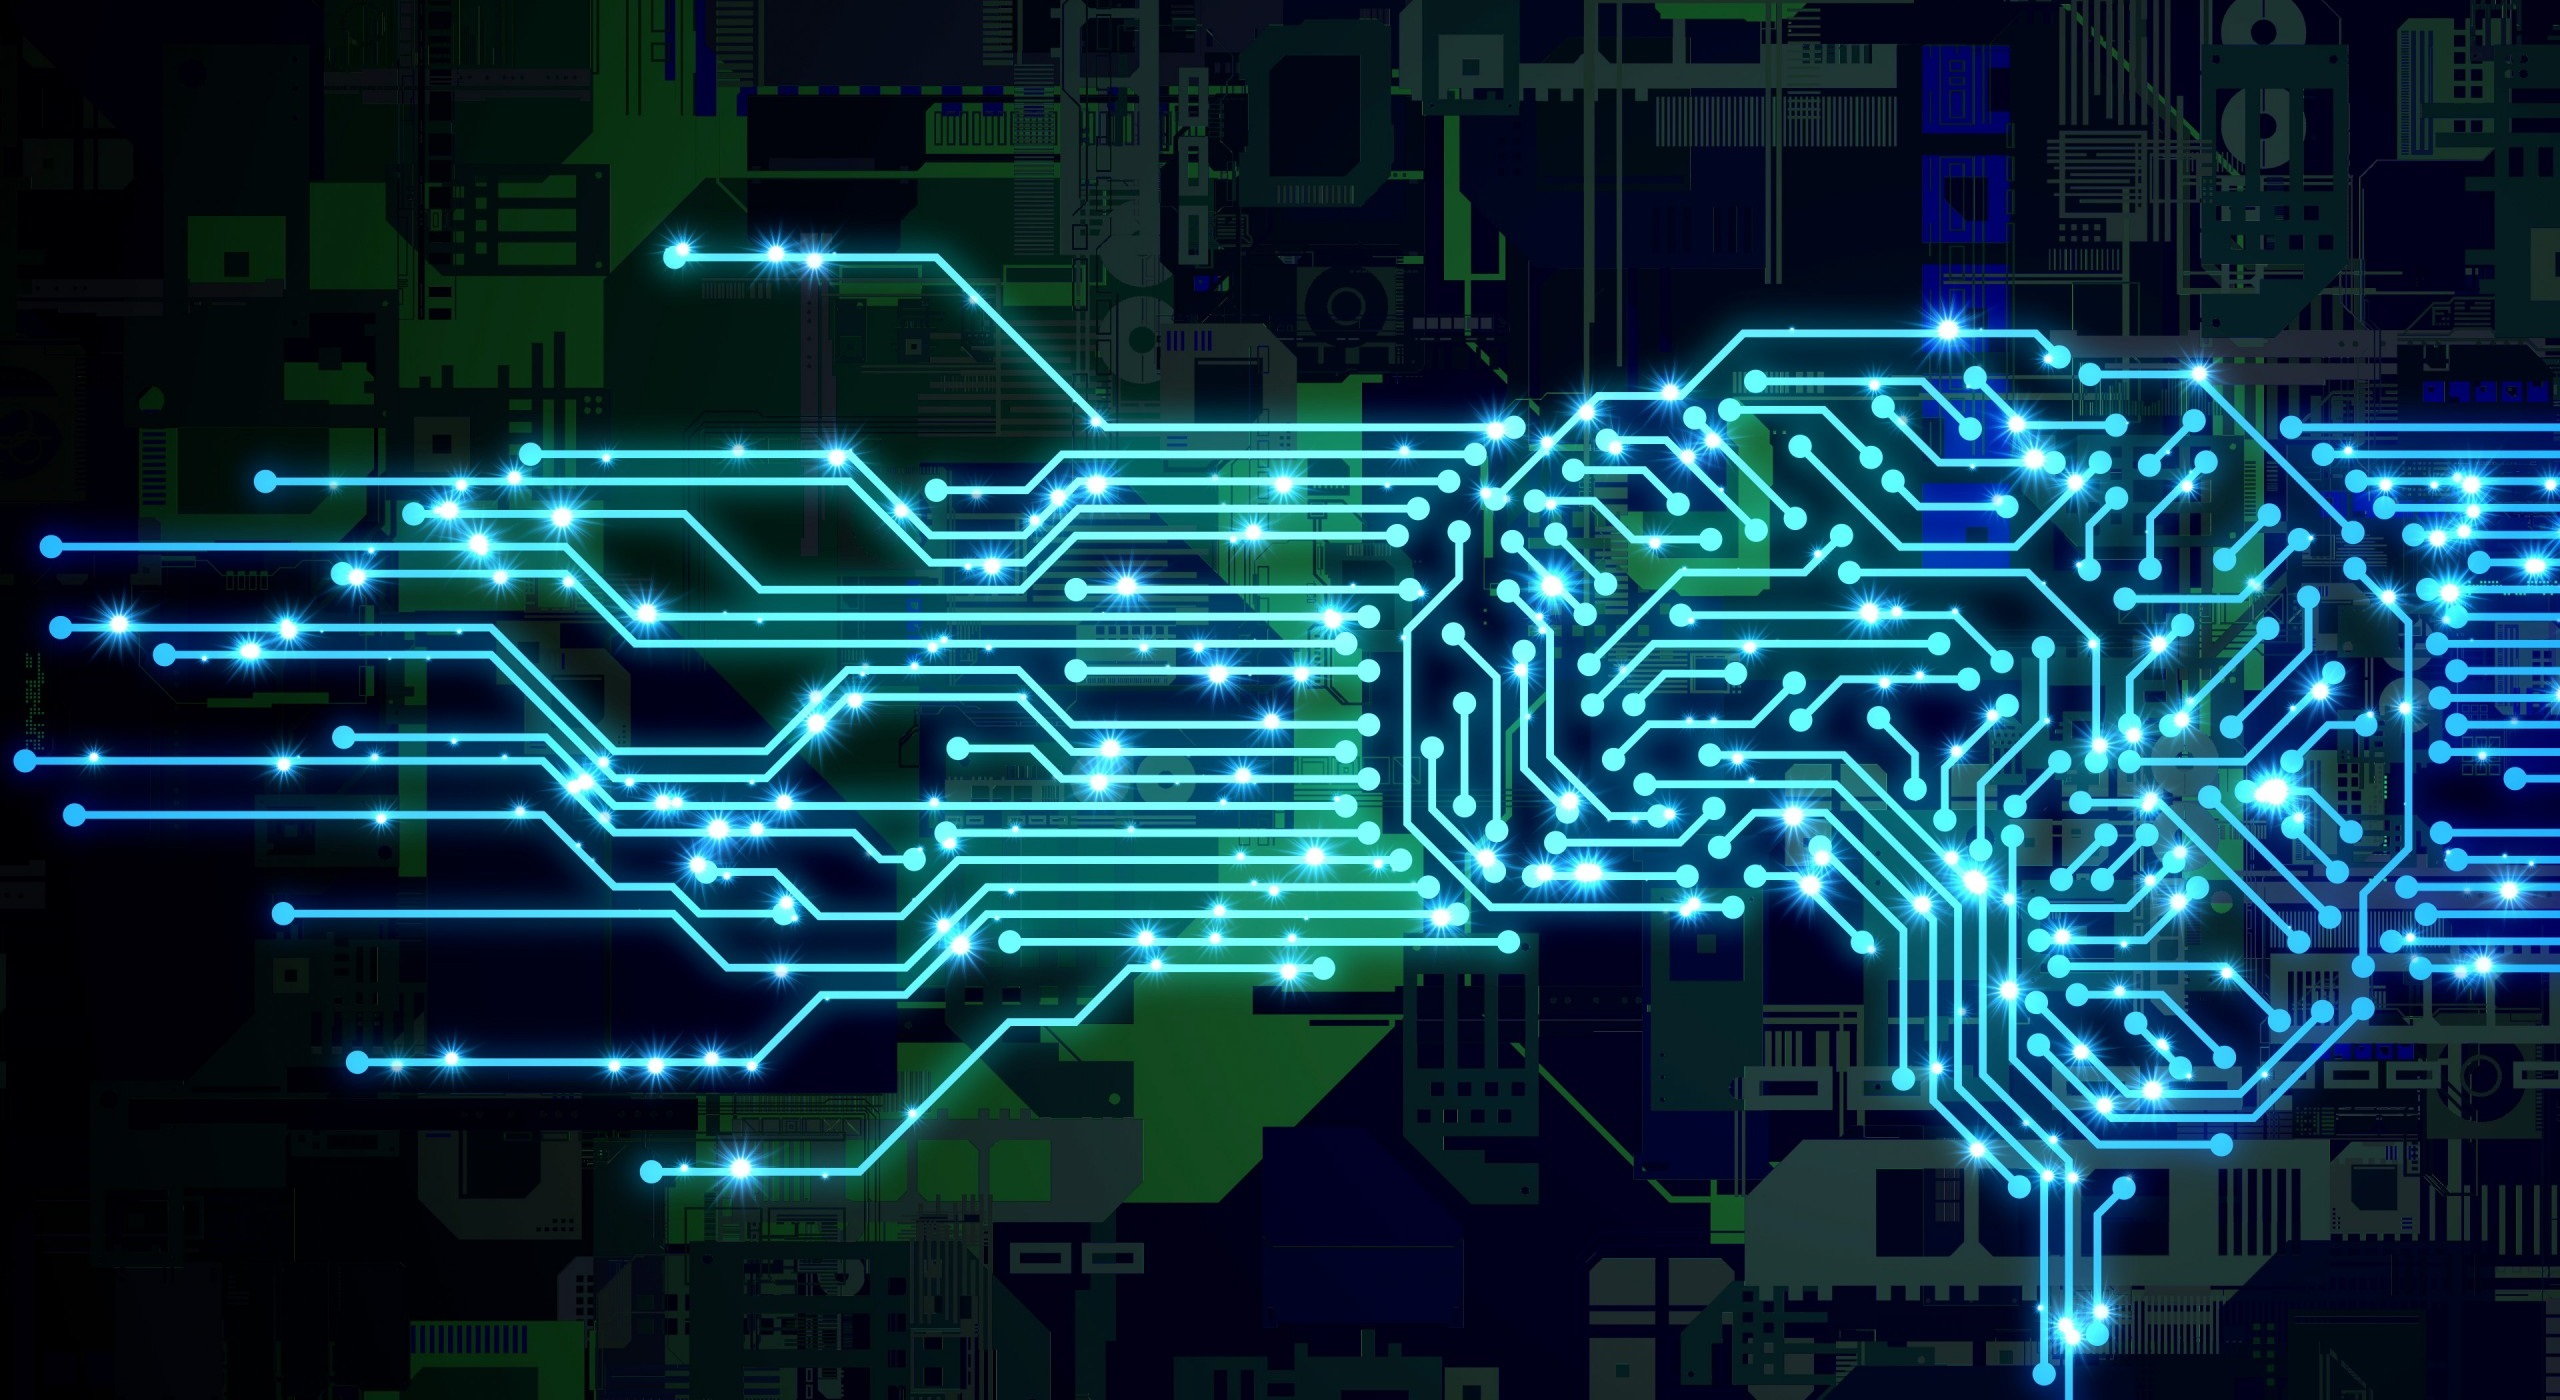
\includegraphics[width=\paperheight,height=\paperwidth,angle=-90]{Cover}};
\begin{center}

\includegraphics[width=245.7px]{LogoUnife.pdf}\vspace{3pt}
\rule[0.1cm]{\textwidth}{0.1mm}
\rule[0.5cm]{\textwidth}{0.6mm}\vspace{-6pt}
{\large\bfseries Dipartimento di Fisica e Scienze della Terra\\
Master Degree in Physics}
\end{center}
\vspace{25mm}
\begin{center}
{\fontsize{30pt}{36pt}\selectfont{\bf {\textsc{Notes of}}}}\vspace{12pt}\\
{\fontsize{30pt}{36pt}\selectfont{\bf {\textsc{Artificial Intelligence}}}}\\
\vspace{22mm}
{\Large\bf
Francesco Tralli\footnote{francesco.tralli@edu.unife.it}\vspace{3pt}\par
Andrea Di Donna\footnote{andrea.didonna@edu.unife.it}\vspace{3pt}\par
Federico Matias Melendi\footnote{federicomati.melendi@edu.unife.it}\par}
\end{center}
\vspace{40mm}
\begin{center}
{\Large{\bf A.Y. 2020/2021}}
\end{center}
\begin{center}
{\large (Last revised \today)}
\end{center}
\end{titlepage}
\restoregeometry



\frontmatter
\bookmarksetupnext{addtohook=\bookmarksetup{color=[RGB]{128,0,0},bold}}
\pdfbookmark[chapter]{\contentsname}{toc}
{\tableofcontents}
\addtocontents{toc}{~\hfill\textbf{Page}\par}


\bookmarksetupnext{addtohook=\bookmarksetup{color={}}}
{\renewcommand{\chaptermark}[1]{\markboth{#1}{}}
\chapter{Preface}
These notes are based on the lectures of Artificial Intelligence (Master Degree in Physics) held by Professor Alessandro Drago at Università degli Studi di Ferrara during the academic year 2020/2021. In addition to the knowledge provided by the professor himself during the course, about a dozen of various texts (books, articles, websites, etc.) have been consulted for the preparation of these notes, in order to make the final result more accurate and complete. The entire list of all references can be easily found at the very end of this document. Nonetheless, the main reference textbooks on which this text is based, as recommended by the professor himself, are:
\begin{enumerate}
\item ``Artificial Intelligence: A Modern Approach'' by S. Russell and P. Norvig~\cite{RussellNorvig3,RussellNorvig4} for the introductory part (Chapter~\ref{chap:1});
\item ``Numerical Recipes: The Art of Scientific Computing'' by W. H. Press et al.~\cite{Recipes} for random number generation and Monte Carlo techniques (Chapter~\ref{chap:2});
\item ``Neural Networks: An Introduction'' by B. Müller, J. Reinhardt, M. T. Strickland~\cite{MRS} for the part of neural networks (Chapter~\ref{chap:3});
\item ``Hands-on Machine Learning with Scikit-Learn, Keras \& TensorFlow'' by Aurélien Géron~\cite{Geron1,Geron2} for the part of neural networks (Chapter~\ref{chap:4}).
\end{enumerate}
Also, the appendix of this book contains a collection of instructive programs taken from~\cite{MRS} and written in C.

Furthermore, in order to make it easier to understand the covered topics, within the text are embedded some examples of codes based on calculation programs such as Python or Mathematica. These are also attached to the pdf file and indicated in the text with a small push pin icon \raisebox{-0.755mm}{
\includegraphics[height=3.4mm]{Push Pin}}. By default setting Adobe Acrobat Reader does not allow you to open or save attachments with particular extensions that can represent a potential security risk. These are, for instance, executable files (\texttt{.exe}), archives (\texttt{.rar}), but also (and unfortunately) Python files (\texttt{.py}) because they are the most suspected type of file to carry malicious contents, open other dangerous file or launch applications. In order to change these settings, follow the procedure indicated at the following link: \url{https://www.adobe.com/devnet-docs/acrobatetk/tools/AppSec/attachments.html?highlight=blacklist}. Nevertheless, unfortunately, these modified settings are restored to the default ones whenever Adobe Acrobat Reader is updated (and blocking automatic updates is quite tricky).

There is at disposal also a great collection of very complicated (and complete) codes from Russell and Norvig~\cite{RussellNorvig3} that covers all the textbook. If you're interested in, you can find them on GitHub, but they have a lot of dependencies, also internal dependencies, so you have to follow the instructions written at the link \url{https://github.com/aimacode/aima-python}.

Instead, the examples taken from Géron~\cite{Geron1,Geron2} are available for consultation at the following link, written also inside the book itself: \url{https://github.com/ageron/handson-ml2}.

Having said that, as exhaustive as they may seem, these notes should be considered as a study support for a better follow-up of the course, and not as a substitute for face-to-face lessons.

%These notes are in constant update and it is therefore possible to find the most recent version at the link shown on the front page; if for some reasons the Google Drive link stops working, just contact me via mail or in person. Another remark is that some old versions of Adobe Acrobat Reader report an error (error code 131) when consulting the file. Although I have not yet fully understood the origin, it is possible to solve it by lowering the pdf version (e.g. from 1.5 to 1.4). Anyway, contact me and I will provide you a working version.

Readers are also strongly encouraged to report \emph{any} kind of error (misprints, misspellings, mistakes) to the author. Of course, any errors that remain are my sole responsibility.



\vspace{1cm}
\hspace*{9.5cm}\emph{Francesco Tralli}\par
\hspace*{9.5cm}\emph{Andrea Di Donna}\par
\hspace*{9.5cm}\emph{Federico Matias Melendi}

\vspace{1cm}
{\centering\pgfornament[scale=0.6]{89}\par}
}



\mainmatter




\titleformat{\chapter}[display]{\normalfont\huge\bfseries\raggedleft}{\textsc{\chaptertitlename}\ \resizebox{!}{1.5cm}{\thechapter}\rlap{\hspace{0.43cm}\raisebox{0.6pt}{\tikz{\fill[left color=black,right color=Background!10!black] (0,0) rectangle (2.57,1.5);}}}}{14pt}{\Huge}
\titlespacing*{\chapter}{0pt}{50pt}{30pt}





\chapter{Problem solving by uninformed and informed search}\label{chap:1}



\section{Intelligent Agent}

\lettrine[lines=3,nindent=0em,loversize=0.5]{A}{n} Agent is a structured entities composed of Sensors and Actuators, trough which it can get information on an Environment, and subsequently this can act on the Environment.




\begin{itemize}
  \item A Rational Agent act in order to obtain the best Results.

  \item The term "percept" indicate perceptive inputs.

  \item The "percept sequence" is the chronological sequence of the perception of the agent.

  \item The behaviour of an agent is described by the "Agent Function" which describes the correspondence between any specific "percept sequence" and the consequent "action".

  \item The "Agent Function" is an abstract mathematical description of the rational agent and thus can be tabulated.

  \item The "Agent Program" is the concrete implementation of the rational agent in a real system.
\end{itemize}


\subsection{Performance measure based on the rationality assumption}
The best results requested to the agent, to be best performing, need a "performance measure", which usually occur to be a distance between answer provided by the agent and the goal itself.

Performance Measure should be structured over the effect that is desirable for the agent to obtain on the ambient, instead of infer about how the agent is supposed to act.

The "rationality" of an agent is based, as Plato taught us, on these parameters:
\begin{itemize}
  \item The knowledge of the ambient;
  \item The action that the agent can take;
  \item The Performance Measure;
  \item The perceptive sequence;
\end{itemize}

In base of these knowledge the Agent must be able to choose an action that maximize the performance measure.

A second kind of action that the agent should be able to do is to Gather Information exploring the Environment, in order to boost its performance.

A third kind of action that the agent should be able to do is to Learn in base of its own perception.

\subsection{Classification of Agent}
\begin{itemize}
  \item \textbf{Simple reflex agent}
    The simplest kind of agent is the simple reflex agent. These agents select actions on the basis of the current percept, ignoring the rest of the percept history.
    it act in base of an condition–action rule stated as:
    if event-happened then start-action
  \item \textbf{Model Based reflex Agent}
  The most effective way to handle partial observability is for the agent to keep track of the part of the world it can’t see now.
  That is, the agent should maintain some sort of internal state that depends on the percept history and thereby reflects at least some of the unobserved aspects of the current state.
  \item \textbf{Goal Based Agent}
  Knowing something about the current state of the environment is not always enough to decide what to do. The GOAL agent needs some sort of goal information that describes situations that are desirable.
  Search and planning are the subfields of AI devoted to finding action sequences that achieve the agent’s goals.
  Although the goal-based agent appears less efficient, it is more flexible because the knowledge that supports its decisions is represented explicitly and can be modified.
  \item \textbf{Utility Based Agent} We have already seen that a performance measure assigns a score to any given sequence of environment states, so it can easily distinguish between more and less desirable ways of getting to the taxi’s destination. An agent’s utility function is essentially an internalization
  of the performance measure. If the internal utility function and the external performance measure are in agreement, then an agent that chooses actions to maximize its utility will be
  rational according to the external performance measure

  \item \textbf{Learning Agent}
  A learning agent can be divided into four conceptual components.
  The most important distinction is between the "Learning Element", which is responsible for making improvements, and the "Performance Element", which is responsible for selecting external actions. The performance element is what we have previously considered
  to be the entire agent: it takes in percepts and decides on actions. The learning element uses feedback from the "Critic" on how the agent is doing and determines how the performance element should be modified to do better in the future.
  The last component of the learning agent is the "problem generator". It is responsible for suggesting actions that will lead to new and informative experiences.
\end{itemize}

\begin{figure}[h!]
\centering
\subfloat[][\emph{Simple Agent}]
{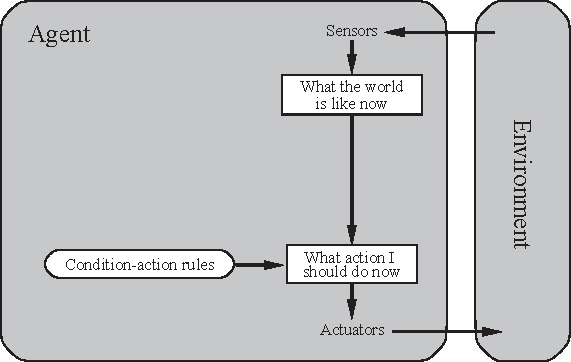
\includegraphics[width=.425\textwidth]{Simple Agent.pdf}} \qquad
\subfloat[][\emph{Goal Based Agent}]
{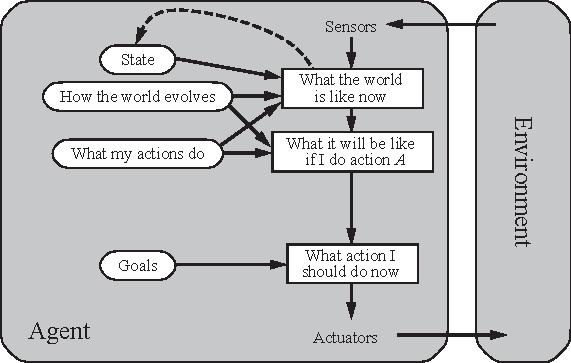
\includegraphics[width=.425\textwidth]{Goal Based.pdf}} \\
\subfloat[][\emph{Model Based Agent}]
{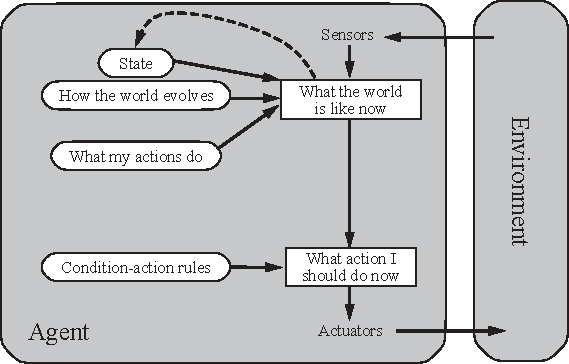
\includegraphics[width=.425\textwidth]{Model Based.pdf}} \qquad
\subfloat[][\emph{Utility Based Agent}]
{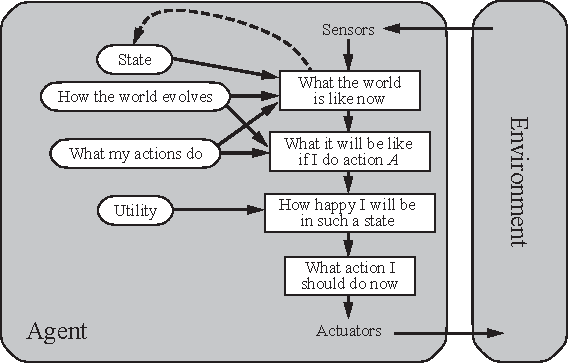
\includegraphics[width=.425\textwidth]{Utility Agent.pdf}}\\
\subfloat[][\emph{Learning Based Agent}]
{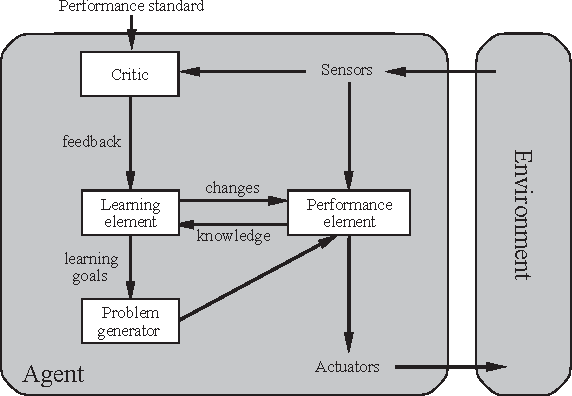
\includegraphics[width=.425\textwidth]{Learning Agent.pdf}}

\caption{Different agent models}
\label{fig:Models}
\end{figure}
%------------------------------------------------
\section{Properties of environments}

Environments come in several flavors. The principal distinctions to be made are as follows:

\begin{itemize}
  \item \textbf{Accessible vs. unaccessible}
  If an agent's sensory apparatus gives it access to the complete state of the environment, then we say that the environment is accessible to that agent. An environment is effectively accessible if the sensors detect all aspects that are relevant to the choice of action. An accessible environment is convenient because the agent need not maintain any internal state to keep track of the world.
  \item \textbf{Deterministic vs. nondeterministic}
  If the next state of the environment is completely determined by the current state and the actions selected by the agents, then we say the environment is deterministic. In principle, an agent need not worry about uncertainty in an accessible, deterministic environment. If the environment is inaccessible, however, then it may appear to be nondeterministic. This is particularly true if the environment is complex, making it hard to keep track of all the inaccessible aspects. Thus, it is often better to think of an environment as deterministic or nondeterministic from the point of view of the agent.
  \item \textbf{Episodic vs. nonepisodic}
  In an episodic environment, the agent's experience is divided into "episodes." Each episode consists of the agent perceiving and then acting. The quality of its action depends just on the episode itself, because subsequent episodes do not depend on what actions occur in previous episodes. Episodic environments are much simpler because the agent does not need to think ahead.
  \item \textbf{Static vs. dynamic}
  If the environment can change while an agent is deliberating, then we say the environment is dynamic for that agent, otherwise it is static. Static environments are easy to deal with because the agent need not keep looking at the world while it is deciding on an action,
  nor need it worry about the passage of time. If the environment does not change with the passage of time but the agent's performance score does, then we say the environment is semidynamic.
  \item \textbf{Discrete vs. continuous.}
  If there are a limited number of distinct, clearly defined percepts and actions we say that the environment is discrete. Chess is discrete—there are a fixed number of possible moves on each turn. Taxi driving is continuous—the speed and location of the taxi and the other vehicles sweep through a range of continuous values.
\end{itemize}

\section{Example problems}
\subsection{Toy problems}
\subsubsection{Missionaries and cannibals}
The missionaries and cannibals problem is usually stated as follows. Three missionaries and three cannibals are on one side of a river, along with a boat that can hold at most two people. The boat cannot cross the river by itself with no people on board. Find a way to get everyone to the other side without ever leaving a group of missionaries in one place outnumbered by the cannibals in that place (if they were, the cannibals would eat the missionaries).

There are basically two ways to solve this problem. The trivial one consists in trying manually until we get the solution (deprecated). A smarter option instead would be to reason about the possible states and legal actions (Fig.~\ref{MissionariesCannibals}). As we did in the previous sections for the vacuum-world, we start with the initial state and we build a tree diagram contemplating all possible transitions from one bank to the other. Obviously, any node that has more cannibals than missionaries on either bank is in an invalid state, and is therefore removed from further consideration. When we find a path that connects the initial states with the final one (all people in the opposite bank), then we've found one possible solution. Naturally, we expect the solutions to be infinite in number because every action can restore the environment to the previous configuration, generating a sort of loop that does not provide any help with the resolution. Nonetheless, it is possible to verify that there are 4 possible shortest solutions, each one requiring 11 boat trips.
\begin{figure}[ht]
\centering
\definecolor{River}{RGB}{51,102,204}
\resizebox{\textwidth}{!}{\newcommand{\scale}{0.36}
\begin{tikzpicture}
%\node[inner sep=0pt,outer sep=0pt] at (7.49,-1.05) {\includegraphics[width=\textwidth]{Missionaries and Cannibals Problem}};
\begin{scope}[scale=\scale,shift={(0,0)}]
\draw[line width=\scale*0.7mm,gray!75] (0.03,0.03) rectangle (5.19,3.47);
\draw[line width=\scale*0.8pt,fill=River,line join=round] plot [] coordinates {
(1.93,0)
(1.93+0.034,3.5*1/64)
(1.93+0.06,3.5*2/64)
(1.93+0.08,3.5*3/64)
(1.93+0.095,3.5*4/64)
(1.93+0.116,3.5*6/64)
(1.93+0.13,3.5*8/64)
(1.93+0.15,3.5*12/64)
(1.93+0.155,3.5*16/64)
(1.93+0.15,3.5*20/64)
(1.93+0.135,3.5*24/64)
(1.93+0.121,3.5*26/64)
(1.93+0.1,3.5*28/64)
(1.93+0.089,3.5*29/64)
(1.93+0.07,3.5*30/64)
(1.93+0.043,3.5*31/64)
(1.93,3.5*32/64)
(1.93-0.043,3.5*33/64)
(1.93-0.07,3.5*34/64)
(1.93-0.089,3.5*35/64)
(1.93-0.1,3.5*36/64)
(1.93-0.121,3.5*38/64)
(1.93-0.135,3.5*40/64)
(1.93-0.15,3.5*44/64)
(1.93-0.155,3.5*48/64)
(1.93-0.15,3.5*52/64)
(1.93-0.13,3.5*56/64)
(1.93-0.116,3.5*58/64)
(1.93-0.095,3.5*60/64)
(1.93-0.08,3.5*61/64)
(1.93-0.06,3.5*62/64)
(1.93-0.034,3.5*63/64)
(1.93,3.5)
(3.29,3.5)
(3.29-0.034,3.5*63/64)
(3.29-0.06,3.5*62/64)
(3.29-0.08,3.5*61/64)
(3.29-0.095,3.5*60/64)
(3.29-0.116,3.5*58/64)
(3.29-0.13,3.5*56/64)
(3.29-0.15,3.5*52/64)
(3.29-0.155,3.5*48/64)
(3.29-0.15,3.5*44/64)
(3.29-0.135,3.5*40/64)
(3.29-0.121,3.5*38/64)
(3.29-0.1,3.5*36/64)
(3.29-0.089,3.5*35/64)
(3.29-0.07,3.5*34/64)
(3.29-0.043,3.5*33/64)
(3.29,3.5*32/64)
(3.29+0.043,3.5*31/64)
(3.29+0.07,3.5*30/64)
(3.29+0.089,3.5*29/64)
(3.29+0.1,3.5*28/64)
(3.29+0.121,3.5*26/64)
(3.29+0.135,3.5*24/64)
(3.29+0.15,3.5*20/64)
(3.29+0.155,3.5*16/64)
(3.29+0.15,3.5*12/64)
(3.29+0.13,3.5*8/64)
(3.29+0.116,3.5*6/64)
(3.29+0.095,3.5*4/64)
(3.29+0.08,3.5*3/64)
(3.29+0.06,3.5*2/64)
(3.29+0.034,3.5*1/64)
(3.29,0)};
\draw[line width=\scale*0.7mm] (0,0) rectangle (5.22,3.5);
\draw[line width=\scale*0.7pt,line join=round,fill=white] (2.005,0.71) -- (2.535,0.71) -- (2.78,1.06) -- (1.76,1.06) -- cycle;
%\draw[line width=\scale*0.7pt,line join=round,fill=white] (3.41,1.75) -- (2.88,1.75) -- (2.635,2.12) -- (3.655,2.12) -- cycle;
\draw[line width=\scale*0.6pt,fill=black] (0.175,1.41) --++ (0:0.37) --++ (120:0.37) -- cycle;
\draw[line width=\scale*0.6pt,fill=black] (0.175+0.52,1.41-0.18) --++ (0:0.37) --++ (120:0.37) -- cycle;
\draw[line width=\scale*0.6pt,fill=black] (0.175+2*0.52,1.41-2*0.18) --++ (0:0.37) --++ (120:0.37) -- cycle;
\draw[line width=\scale*0.6pt,fill=red] (0.53,0.885) circle (0.174);
\draw[line width=\scale*0.6pt,fill=red] (0.53+0.52,0.885-0.18) circle (0.174);
\draw[line width=\scale*0.6pt,fill=red] (0.53+2*0.52,0.885-2*0.18) circle (0.174);
%\draw[line width=\scale*0.6pt,fill=black] (3.455,2.95) --++ (0:0.37) --++ (120:0.37) -- cycle;
%\draw[line width=\scale*0.6pt,fill=black] (3.455+0.52,2.95-0.18) --++ (0:0.37) --++ (120:0.37) -- cycle;
%\draw[line width=\scale*0.6pt,fill=black] (3.455+2*0.52,2.95-2*0.18) --++ (0:0.37) --++ (120:0.37) -- cycle;
%\draw[line width=\scale*0.6pt,fill=red] (3.81,2.425) circle (0.174);
%\draw[line width=\scale*0.6pt,fill=red] (3.81+0.52,2.425-0.18) circle (0.174);
%\draw[line width=\scale*0.6pt,fill=red] (3.81+2*0.52,2.425-2*0.18) circle (0.174);
\end{scope}
%%%%%%%%%%%%%%%%%%%%%%%%%%%%%%%%%%%%%%%%%%%%%%%%%%%%%
\begin{scope}[scale=\scale,shift={(6.76,0)}]
\draw[line width=\scale*0.7mm,gray!75] (0.03,0.03) rectangle (5.19,3.47);
\draw[line width=\scale*0.8pt,fill=River,line join=round] plot [] coordinates {
(1.93,0)
(1.93+0.034,3.5*1/64)
(1.93+0.06,3.5*2/64)
(1.93+0.08,3.5*3/64)
(1.93+0.095,3.5*4/64)
(1.93+0.116,3.5*6/64)
(1.93+0.13,3.5*8/64)
(1.93+0.15,3.5*12/64)
(1.93+0.155,3.5*16/64)
(1.93+0.15,3.5*20/64)
(1.93+0.135,3.5*24/64)
(1.93+0.121,3.5*26/64)
(1.93+0.1,3.5*28/64)
(1.93+0.089,3.5*29/64)
(1.93+0.07,3.5*30/64)
(1.93+0.043,3.5*31/64)
(1.93,3.5*32/64)
(1.93-0.043,3.5*33/64)
(1.93-0.07,3.5*34/64)
(1.93-0.089,3.5*35/64)
(1.93-0.1,3.5*36/64)
(1.93-0.121,3.5*38/64)
(1.93-0.135,3.5*40/64)
(1.93-0.15,3.5*44/64)
(1.93-0.155,3.5*48/64)
(1.93-0.15,3.5*52/64)
(1.93-0.13,3.5*56/64)
(1.93-0.116,3.5*58/64)
(1.93-0.095,3.5*60/64)
(1.93-0.08,3.5*61/64)
(1.93-0.06,3.5*62/64)
(1.93-0.034,3.5*63/64)
(1.93,3.5)
(3.29,3.5)
(3.29-0.034,3.5*63/64)
(3.29-0.06,3.5*62/64)
(3.29-0.08,3.5*61/64)
(3.29-0.095,3.5*60/64)
(3.29-0.116,3.5*58/64)
(3.29-0.13,3.5*56/64)
(3.29-0.15,3.5*52/64)
(3.29-0.155,3.5*48/64)
(3.29-0.15,3.5*44/64)
(3.29-0.135,3.5*40/64)
(3.29-0.121,3.5*38/64)
(3.29-0.1,3.5*36/64)
(3.29-0.089,3.5*35/64)
(3.29-0.07,3.5*34/64)
(3.29-0.043,3.5*33/64)
(3.29,3.5*32/64)
(3.29+0.043,3.5*31/64)
(3.29+0.07,3.5*30/64)
(3.29+0.089,3.5*29/64)
(3.29+0.1,3.5*28/64)
(3.29+0.121,3.5*26/64)
(3.29+0.135,3.5*24/64)
(3.29+0.15,3.5*20/64)
(3.29+0.155,3.5*16/64)
(3.29+0.15,3.5*12/64)
(3.29+0.13,3.5*8/64)
(3.29+0.116,3.5*6/64)
(3.29+0.095,3.5*4/64)
(3.29+0.08,3.5*3/64)
(3.29+0.06,3.5*2/64)
(3.29+0.034,3.5*1/64)
(3.29,0)};
\draw[line width=\scale*0.7mm] (0,0) rectangle (5.22,3.5);
\draw[line width=\scale*0.7pt,line join=round,fill=white] (3.41,1.75) -- (2.88,1.75) -- (2.635,2.12) -- (3.655,2.12) -- cycle;
\draw[line width=\scale*0.6pt,fill=black] (0.175+0.52,1.41-0.18) --++ (0:0.37) --++ (120:0.37) -- cycle;
\draw[line width=\scale*0.6pt,fill=black] (0.175+2*0.52,1.41-2*0.18) --++ (0:0.37) --++ (120:0.37) -- cycle;
\draw[line width=\scale*0.6pt,fill=red] (0.53+0.52,0.885-0.18) circle (0.174);
\draw[line width=\scale*0.6pt,fill=red] (0.53+2*0.52,0.885-2*0.18) circle (0.174);
\draw[line width=\scale*0.6pt,fill=black] (3.455,2.95) --++ (0:0.37) --++ (120:0.37) -- cycle;
\draw[line width=\scale*0.6pt,fill=red] (3.81,2.425) circle (0.174);
\end{scope}
%%%%%%%%%%%%%%%%%%%%%%%%%%%%%%%%%%%%%%%%%%%%%%%%%%%%%
\begin{scope}[scale=\scale,shift={(6.76,4.15)}]
\draw[line width=\scale*0.7mm,gray!75] (0.03,0.03) rectangle (5.19,3.47);
\draw[line width=\scale*0.8pt,fill=River,line join=round] plot [] coordinates {
(1.93,0)
(1.93+0.034,3.5*1/64)
(1.93+0.06,3.5*2/64)
(1.93+0.08,3.5*3/64)
(1.93+0.095,3.5*4/64)
(1.93+0.116,3.5*6/64)
(1.93+0.13,3.5*8/64)
(1.93+0.15,3.5*12/64)
(1.93+0.155,3.5*16/64)
(1.93+0.15,3.5*20/64)
(1.93+0.135,3.5*24/64)
(1.93+0.121,3.5*26/64)
(1.93+0.1,3.5*28/64)
(1.93+0.089,3.5*29/64)
(1.93+0.07,3.5*30/64)
(1.93+0.043,3.5*31/64)
(1.93,3.5*32/64)
(1.93-0.043,3.5*33/64)
(1.93-0.07,3.5*34/64)
(1.93-0.089,3.5*35/64)
(1.93-0.1,3.5*36/64)
(1.93-0.121,3.5*38/64)
(1.93-0.135,3.5*40/64)
(1.93-0.15,3.5*44/64)
(1.93-0.155,3.5*48/64)
(1.93-0.15,3.5*52/64)
(1.93-0.13,3.5*56/64)
(1.93-0.116,3.5*58/64)
(1.93-0.095,3.5*60/64)
(1.93-0.08,3.5*61/64)
(1.93-0.06,3.5*62/64)
(1.93-0.034,3.5*63/64)
(1.93,3.5)
(3.29,3.5)
(3.29-0.034,3.5*63/64)
(3.29-0.06,3.5*62/64)
(3.29-0.08,3.5*61/64)
(3.29-0.095,3.5*60/64)
(3.29-0.116,3.5*58/64)
(3.29-0.13,3.5*56/64)
(3.29-0.15,3.5*52/64)
(3.29-0.155,3.5*48/64)
(3.29-0.15,3.5*44/64)
(3.29-0.135,3.5*40/64)
(3.29-0.121,3.5*38/64)
(3.29-0.1,3.5*36/64)
(3.29-0.089,3.5*35/64)
(3.29-0.07,3.5*34/64)
(3.29-0.043,3.5*33/64)
(3.29,3.5*32/64)
(3.29+0.043,3.5*31/64)
(3.29+0.07,3.5*30/64)
(3.29+0.089,3.5*29/64)
(3.29+0.1,3.5*28/64)
(3.29+0.121,3.5*26/64)
(3.29+0.135,3.5*24/64)
(3.29+0.15,3.5*20/64)
(3.29+0.155,3.5*16/64)
(3.29+0.15,3.5*12/64)
(3.29+0.13,3.5*8/64)
(3.29+0.116,3.5*6/64)
(3.29+0.095,3.5*4/64)
(3.29+0.08,3.5*3/64)
(3.29+0.06,3.5*2/64)
(3.29+0.034,3.5*1/64)
(3.29,0)};
\draw[line width=\scale*0.7mm] (0,0) rectangle (5.22,3.5);
\draw[line width=\scale*0.7pt,line join=round,fill=white] (3.41,1.75) -- (2.88,1.75) -- (2.635,2.12) -- (3.655,2.12) -- cycle;
\draw[line width=\scale*0.6pt,fill=black] (0.175,1.41) --++ (0:0.37) --++ (120:0.37) -- cycle;
\draw[line width=\scale*0.6pt,fill=black] (0.175+0.52,1.41-0.18) --++ (0:0.37) --++ (120:0.37) -- cycle;
\draw[line width=\scale*0.6pt,fill=black] (0.175+2*0.52,1.41-2*0.18) --++ (0:0.37) --++ (120:0.37) -- cycle;
\draw[line width=\scale*0.6pt,fill=red] (0.53+2*0.52,0.885-2*0.18) circle (0.174);
\draw[line width=\scale*0.6pt,fill=red] (3.81,2.425) circle (0.174);
\draw[line width=\scale*0.6pt,fill=red] (3.81+0.52,2.425-0.18) circle (0.174);
\end{scope}
%%%%%%%%%%%%%%%%%%%%%%%%%%%%%%%%%%%%%%%%%%%%%%%%%%%%%
\begin{scope}[scale=\scale,shift={(6.76,-4.15)}]
\draw[line width=\scale*0.7mm,gray!75] (0.03,0.03) rectangle (5.19,3.47);
\draw[line width=\scale*0.8pt,fill=River,line join=round] plot [] coordinates {
(1.93,0)
(1.93+0.034,3.5*1/64)
(1.93+0.06,3.5*2/64)
(1.93+0.08,3.5*3/64)
(1.93+0.095,3.5*4/64)
(1.93+0.116,3.5*6/64)
(1.93+0.13,3.5*8/64)
(1.93+0.15,3.5*12/64)
(1.93+0.155,3.5*16/64)
(1.93+0.15,3.5*20/64)
(1.93+0.135,3.5*24/64)
(1.93+0.121,3.5*26/64)
(1.93+0.1,3.5*28/64)
(1.93+0.089,3.5*29/64)
(1.93+0.07,3.5*30/64)
(1.93+0.043,3.5*31/64)
(1.93,3.5*32/64)
(1.93-0.043,3.5*33/64)
(1.93-0.07,3.5*34/64)
(1.93-0.089,3.5*35/64)
(1.93-0.1,3.5*36/64)
(1.93-0.121,3.5*38/64)
(1.93-0.135,3.5*40/64)
(1.93-0.15,3.5*44/64)
(1.93-0.155,3.5*48/64)
(1.93-0.15,3.5*52/64)
(1.93-0.13,3.5*56/64)
(1.93-0.116,3.5*58/64)
(1.93-0.095,3.5*60/64)
(1.93-0.08,3.5*61/64)
(1.93-0.06,3.5*62/64)
(1.93-0.034,3.5*63/64)
(1.93,3.5)
(3.29,3.5)
(3.29-0.034,3.5*63/64)
(3.29-0.06,3.5*62/64)
(3.29-0.08,3.5*61/64)
(3.29-0.095,3.5*60/64)
(3.29-0.116,3.5*58/64)
(3.29-0.13,3.5*56/64)
(3.29-0.15,3.5*52/64)
(3.29-0.155,3.5*48/64)
(3.29-0.15,3.5*44/64)
(3.29-0.135,3.5*40/64)
(3.29-0.121,3.5*38/64)
(3.29-0.1,3.5*36/64)
(3.29-0.089,3.5*35/64)
(3.29-0.07,3.5*34/64)
(3.29-0.043,3.5*33/64)
(3.29,3.5*32/64)
(3.29+0.043,3.5*31/64)
(3.29+0.07,3.5*30/64)
(3.29+0.089,3.5*29/64)
(3.29+0.1,3.5*28/64)
(3.29+0.121,3.5*26/64)
(3.29+0.135,3.5*24/64)
(3.29+0.15,3.5*20/64)
(3.29+0.155,3.5*16/64)
(3.29+0.15,3.5*12/64)
(3.29+0.13,3.5*8/64)
(3.29+0.116,3.5*6/64)
(3.29+0.095,3.5*4/64)
(3.29+0.08,3.5*3/64)
(3.29+0.06,3.5*2/64)
(3.29+0.034,3.5*1/64)
(3.29,0)};
\draw[line width=\scale*0.7mm] (0,0) rectangle (5.22,3.5);
\draw[line width=\scale*0.7pt,line join=round,fill=white] (3.41,1.75) -- (2.88,1.75) -- (2.635,2.12) -- (3.655,2.12) -- cycle;
\draw[line width=\scale*0.6pt,fill=black] (0.175,1.41) --++ (0:0.37) --++ (120:0.37) -- cycle;
\draw[line width=\scale*0.6pt,fill=black] (0.175+0.52,1.41-0.18) --++ (0:0.37) --++ (120:0.37) -- cycle;
\draw[line width=\scale*0.6pt,fill=black] (0.175+2*0.52,1.41-2*0.18) --++ (0:0.37) --++ (120:0.37) -- cycle;
\draw[line width=\scale*0.6pt,fill=red] (0.53+0.52,0.885-0.18) circle (0.174);
\draw[line width=\scale*0.6pt,fill=red] (0.53+2*0.52,0.885-2*0.18) circle (0.174);
\draw[line width=\scale*0.6pt,fill=red] (3.81,2.425) circle (0.174);
\end{scope}
%%%%%%%%%%%%%%%%%%%%%%%%%%%%%%%%%%%%%%%%%%%%%%%%%%%%%
\begin{scope}[scale=\scale,shift={(13.52,2.1)}]
\draw[line width=\scale*0.7mm,gray!75] (0.03,0.03) rectangle (5.19,3.47);
\draw[line width=\scale*0.8pt,fill=River,line join=round] plot [] coordinates {
(1.93,0)
(1.93+0.034,3.5*1/64)
(1.93+0.06,3.5*2/64)
(1.93+0.08,3.5*3/64)
(1.93+0.095,3.5*4/64)
(1.93+0.116,3.5*6/64)
(1.93+0.13,3.5*8/64)
(1.93+0.15,3.5*12/64)
(1.93+0.155,3.5*16/64)
(1.93+0.15,3.5*20/64)
(1.93+0.135,3.5*24/64)
(1.93+0.121,3.5*26/64)
(1.93+0.1,3.5*28/64)
(1.93+0.089,3.5*29/64)
(1.93+0.07,3.5*30/64)
(1.93+0.043,3.5*31/64)
(1.93,3.5*32/64)
(1.93-0.043,3.5*33/64)
(1.93-0.07,3.5*34/64)
(1.93-0.089,3.5*35/64)
(1.93-0.1,3.5*36/64)
(1.93-0.121,3.5*38/64)
(1.93-0.135,3.5*40/64)
(1.93-0.15,3.5*44/64)
(1.93-0.155,3.5*48/64)
(1.93-0.15,3.5*52/64)
(1.93-0.13,3.5*56/64)
(1.93-0.116,3.5*58/64)
(1.93-0.095,3.5*60/64)
(1.93-0.08,3.5*61/64)
(1.93-0.06,3.5*62/64)
(1.93-0.034,3.5*63/64)
(1.93,3.5)
(3.29,3.5)
(3.29-0.034,3.5*63/64)
(3.29-0.06,3.5*62/64)
(3.29-0.08,3.5*61/64)
(3.29-0.095,3.5*60/64)
(3.29-0.116,3.5*58/64)
(3.29-0.13,3.5*56/64)
(3.29-0.15,3.5*52/64)
(3.29-0.155,3.5*48/64)
(3.29-0.15,3.5*44/64)
(3.29-0.135,3.5*40/64)
(3.29-0.121,3.5*38/64)
(3.29-0.1,3.5*36/64)
(3.29-0.089,3.5*35/64)
(3.29-0.07,3.5*34/64)
(3.29-0.043,3.5*33/64)
(3.29,3.5*32/64)
(3.29+0.043,3.5*31/64)
(3.29+0.07,3.5*30/64)
(3.29+0.089,3.5*29/64)
(3.29+0.1,3.5*28/64)
(3.29+0.121,3.5*26/64)
(3.29+0.135,3.5*24/64)
(3.29+0.15,3.5*20/64)
(3.29+0.155,3.5*16/64)
(3.29+0.15,3.5*12/64)
(3.29+0.13,3.5*8/64)
(3.29+0.116,3.5*6/64)
(3.29+0.095,3.5*4/64)
(3.29+0.08,3.5*3/64)
(3.29+0.06,3.5*2/64)
(3.29+0.034,3.5*1/64)
(3.29,0)};
\draw[line width=\scale*0.7mm] (0,0) rectangle (5.22,3.5);
\draw[line width=\scale*0.7pt,line join=round,fill=white] (2.005,0.71) -- (2.535,0.71) -- (2.78,1.06) -- (1.76,1.06) -- cycle;
\draw[line width=\scale*0.6pt,fill=black] (0.175,1.41) --++ (0:0.37) --++ (120:0.37) -- cycle;
\draw[line width=\scale*0.6pt,fill=black] (0.175+0.52,1.41-0.18) --++ (0:0.37) --++ (120:0.37) -- cycle;
\draw[line width=\scale*0.6pt,fill=black] (0.175+2*0.52,1.41-2*0.18) --++ (0:0.37) --++ (120:0.37) -- cycle;
\draw[line width=\scale*0.6pt,fill=red] (0.53+0.52,0.885-0.18) circle (0.174);
\draw[line width=\scale*0.6pt,fill=red] (0.53+2*0.52,0.885-2*0.18) circle (0.174);
\draw[line width=\scale*0.6pt,fill=red] (3.81,2.425) circle (0.174);
\end{scope}
%%%%%%%%%%%%%%%%%%%%%%%%%%%%%%%%%%%%%%%%%%%%%%%%%%%%%
\begin{scope}[scale=\scale,shift={(13.98,-3.09)}]
\draw[line width=\scale*0.7mm,gray!75] (0.03,0.03) rectangle (5.19,3.47);
\draw[line width=\scale*0.8pt,fill=River,line join=round] plot [] coordinates {
(1.93,0)
(1.93+0.034,3.5*1/64)
(1.93+0.06,3.5*2/64)
(1.93+0.08,3.5*3/64)
(1.93+0.095,3.5*4/64)
(1.93+0.116,3.5*6/64)
(1.93+0.13,3.5*8/64)
(1.93+0.15,3.5*12/64)
(1.93+0.155,3.5*16/64)
(1.93+0.15,3.5*20/64)
(1.93+0.135,3.5*24/64)
(1.93+0.121,3.5*26/64)
(1.93+0.1,3.5*28/64)
(1.93+0.089,3.5*29/64)
(1.93+0.07,3.5*30/64)
(1.93+0.043,3.5*31/64)
(1.93,3.5*32/64)
(1.93-0.043,3.5*33/64)
(1.93-0.07,3.5*34/64)
(1.93-0.089,3.5*35/64)
(1.93-0.1,3.5*36/64)
(1.93-0.121,3.5*38/64)
(1.93-0.135,3.5*40/64)
(1.93-0.15,3.5*44/64)
(1.93-0.155,3.5*48/64)
(1.93-0.15,3.5*52/64)
(1.93-0.13,3.5*56/64)
(1.93-0.116,3.5*58/64)
(1.93-0.095,3.5*60/64)
(1.93-0.08,3.5*61/64)
(1.93-0.06,3.5*62/64)
(1.93-0.034,3.5*63/64)
(1.93,3.5)
(3.29,3.5)
(3.29-0.034,3.5*63/64)
(3.29-0.06,3.5*62/64)
(3.29-0.08,3.5*61/64)
(3.29-0.095,3.5*60/64)
(3.29-0.116,3.5*58/64)
(3.29-0.13,3.5*56/64)
(3.29-0.15,3.5*52/64)
(3.29-0.155,3.5*48/64)
(3.29-0.15,3.5*44/64)
(3.29-0.135,3.5*40/64)
(3.29-0.121,3.5*38/64)
(3.29-0.1,3.5*36/64)
(3.29-0.089,3.5*35/64)
(3.29-0.07,3.5*34/64)
(3.29-0.043,3.5*33/64)
(3.29,3.5*32/64)
(3.29+0.043,3.5*31/64)
(3.29+0.07,3.5*30/64)
(3.29+0.089,3.5*29/64)
(3.29+0.1,3.5*28/64)
(3.29+0.121,3.5*26/64)
(3.29+0.135,3.5*24/64)
(3.29+0.15,3.5*20/64)
(3.29+0.155,3.5*16/64)
(3.29+0.15,3.5*12/64)
(3.29+0.13,3.5*8/64)
(3.29+0.116,3.5*6/64)
(3.29+0.095,3.5*4/64)
(3.29+0.08,3.5*3/64)
(3.29+0.06,3.5*2/64)
(3.29+0.034,3.5*1/64)
(3.29,0)};
\draw[line width=\scale*0.7mm] (0,0) rectangle (5.22,3.5);
\draw[line width=\scale*0.7pt,line join=round,fill=white] (3.41,1.75) -- (2.88,1.75) -- (2.635,2.12) -- (3.655,2.12) -- cycle;
\draw[line width=\scale*0.6pt,fill=black] (0.175,1.41) --++ (0:0.37) --++ (120:0.37) -- cycle;
\draw[line width=\scale*0.6pt,fill=black] (0.175+0.52,1.41-0.18) --++ (0:0.37) --++ (120:0.37) -- cycle;
\draw[line width=\scale*0.6pt,fill=black] (0.175+2*0.52,1.41-2*0.18) --++ (0:0.37) --++ (120:0.37) -- cycle;
\draw[line width=\scale*0.6pt,fill=red] (3.81,2.425) circle (0.174);
\draw[line width=\scale*0.6pt,fill=red] (3.81+0.52,2.425-0.18) circle (0.174);
\draw[line width=\scale*0.6pt,fill=red] (3.81+2*0.52,2.425-2*0.18) circle (0.174);
\end{scope}
%%%%%%%%%%%%%%%%%%%%%%%%%%%%%%%%%%%%%%%%%%%%%%%%%%%%%
\begin{scope}[scale=\scale,shift={(14.44,-8.28)}]
\draw[line width=\scale*0.7mm,gray!75] (0.03,0.03) rectangle (5.19,3.47);
\draw[line width=\scale*0.8pt,fill=River,line join=round] plot [] coordinates {
(1.93,0)
(1.93+0.034,3.5*1/64)
(1.93+0.06,3.5*2/64)
(1.93+0.08,3.5*3/64)
(1.93+0.095,3.5*4/64)
(1.93+0.116,3.5*6/64)
(1.93+0.13,3.5*8/64)
(1.93+0.15,3.5*12/64)
(1.93+0.155,3.5*16/64)
(1.93+0.15,3.5*20/64)
(1.93+0.135,3.5*24/64)
(1.93+0.121,3.5*26/64)
(1.93+0.1,3.5*28/64)
(1.93+0.089,3.5*29/64)
(1.93+0.07,3.5*30/64)
(1.93+0.043,3.5*31/64)
(1.93,3.5*32/64)
(1.93-0.043,3.5*33/64)
(1.93-0.07,3.5*34/64)
(1.93-0.089,3.5*35/64)
(1.93-0.1,3.5*36/64)
(1.93-0.121,3.5*38/64)
(1.93-0.135,3.5*40/64)
(1.93-0.15,3.5*44/64)
(1.93-0.155,3.5*48/64)
(1.93-0.15,3.5*52/64)
(1.93-0.13,3.5*56/64)
(1.93-0.116,3.5*58/64)
(1.93-0.095,3.5*60/64)
(1.93-0.08,3.5*61/64)
(1.93-0.06,3.5*62/64)
(1.93-0.034,3.5*63/64)
(1.93,3.5)
(3.29,3.5)
(3.29-0.034,3.5*63/64)
(3.29-0.06,3.5*62/64)
(3.29-0.08,3.5*61/64)
(3.29-0.095,3.5*60/64)
(3.29-0.116,3.5*58/64)
(3.29-0.13,3.5*56/64)
(3.29-0.15,3.5*52/64)
(3.29-0.155,3.5*48/64)
(3.29-0.15,3.5*44/64)
(3.29-0.135,3.5*40/64)
(3.29-0.121,3.5*38/64)
(3.29-0.1,3.5*36/64)
(3.29-0.089,3.5*35/64)
(3.29-0.07,3.5*34/64)
(3.29-0.043,3.5*33/64)
(3.29,3.5*32/64)
(3.29+0.043,3.5*31/64)
(3.29+0.07,3.5*30/64)
(3.29+0.089,3.5*29/64)
(3.29+0.1,3.5*28/64)
(3.29+0.121,3.5*26/64)
(3.29+0.135,3.5*24/64)
(3.29+0.15,3.5*20/64)
(3.29+0.155,3.5*16/64)
(3.29+0.15,3.5*12/64)
(3.29+0.13,3.5*8/64)
(3.29+0.116,3.5*6/64)
(3.29+0.095,3.5*4/64)
(3.29+0.08,3.5*3/64)
(3.29+0.06,3.5*2/64)
(3.29+0.034,3.5*1/64)
(3.29,0)};
\draw[line width=\scale*0.7mm] (0,0) rectangle (5.22,3.5);
\draw[line width=\scale*0.7pt,line join=round,fill=white] (2.005,0.71) -- (2.535,0.71) -- (2.78,1.06) -- (1.76,1.06) -- cycle;
\draw[line width=\scale*0.6pt,fill=black] (0.175,1.41) --++ (0:0.37) --++ (120:0.37) -- cycle;
\draw[line width=\scale*0.6pt,fill=black] (0.175+0.52,1.41-0.18) --++ (0:0.37) --++ (120:0.37) -- cycle;
\draw[line width=\scale*0.6pt,fill=black] (0.175+2*0.52,1.41-2*0.18) --++ (0:0.37) --++ (120:0.37) -- cycle;
\draw[line width=\scale*0.6pt,fill=red] (0.53+2*0.52,0.885-2*0.18) circle (0.174);
\draw[line width=\scale*0.6pt,fill=red] (3.81+0.52,2.425-0.18) circle (0.174);
\draw[line width=\scale*0.6pt,fill=red] (3.81+2*0.52,2.425-2*0.18) circle (0.174);
\end{scope}
%%%%%%%%%%%%%%%%%%%%%%%%%%%%%%%%%%%%%%%%%%%%%%%%%%%%%
\begin{scope}[scale=\scale,shift={(14.9,-13.47)}]
\draw[line width=\scale*0.7mm,gray!75] (0.03,0.03) rectangle (5.19,3.47);
\draw[line width=\scale*0.8pt,fill=River,line join=round] plot [] coordinates {
(1.93,0)
(1.93+0.034,3.5*1/64)
(1.93+0.06,3.5*2/64)
(1.93+0.08,3.5*3/64)
(1.93+0.095,3.5*4/64)
(1.93+0.116,3.5*6/64)
(1.93+0.13,3.5*8/64)
(1.93+0.15,3.5*12/64)
(1.93+0.155,3.5*16/64)
(1.93+0.15,3.5*20/64)
(1.93+0.135,3.5*24/64)
(1.93+0.121,3.5*26/64)
(1.93+0.1,3.5*28/64)
(1.93+0.089,3.5*29/64)
(1.93+0.07,3.5*30/64)
(1.93+0.043,3.5*31/64)
(1.93,3.5*32/64)
(1.93-0.043,3.5*33/64)
(1.93-0.07,3.5*34/64)
(1.93-0.089,3.5*35/64)
(1.93-0.1,3.5*36/64)
(1.93-0.121,3.5*38/64)
(1.93-0.135,3.5*40/64)
(1.93-0.15,3.5*44/64)
(1.93-0.155,3.5*48/64)
(1.93-0.15,3.5*52/64)
(1.93-0.13,3.5*56/64)
(1.93-0.116,3.5*58/64)
(1.93-0.095,3.5*60/64)
(1.93-0.08,3.5*61/64)
(1.93-0.06,3.5*62/64)
(1.93-0.034,3.5*63/64)
(1.93,3.5)
(3.29,3.5)
(3.29-0.034,3.5*63/64)
(3.29-0.06,3.5*62/64)
(3.29-0.08,3.5*61/64)
(3.29-0.095,3.5*60/64)
(3.29-0.116,3.5*58/64)
(3.29-0.13,3.5*56/64)
(3.29-0.15,3.5*52/64)
(3.29-0.155,3.5*48/64)
(3.29-0.15,3.5*44/64)
(3.29-0.135,3.5*40/64)
(3.29-0.121,3.5*38/64)
(3.29-0.1,3.5*36/64)
(3.29-0.089,3.5*35/64)
(3.29-0.07,3.5*34/64)
(3.29-0.043,3.5*33/64)
(3.29,3.5*32/64)
(3.29+0.043,3.5*31/64)
(3.29+0.07,3.5*30/64)
(3.29+0.089,3.5*29/64)
(3.29+0.1,3.5*28/64)
(3.29+0.121,3.5*26/64)
(3.29+0.135,3.5*24/64)
(3.29+0.15,3.5*20/64)
(3.29+0.155,3.5*16/64)
(3.29+0.15,3.5*12/64)
(3.29+0.13,3.5*8/64)
(3.29+0.116,3.5*6/64)
(3.29+0.095,3.5*4/64)
(3.29+0.08,3.5*3/64)
(3.29+0.06,3.5*2/64)
(3.29+0.034,3.5*1/64)
(3.29,0)};
\draw[line width=\scale*0.7mm] (0,0) rectangle (5.22,3.5);
\draw[line width=\scale*0.7pt,line join=round,fill=white] (3.41,1.75) -- (2.88,1.75) -- (2.635,2.12) -- (3.655,2.12) -- cycle;
\draw[line width=\scale*0.6pt,fill=black] (0.175+2*0.52,1.41-2*0.18) --++ (0:0.37) --++ (120:0.37) -- cycle;
\draw[line width=\scale*0.6pt,fill=red] (0.53+2*0.52,0.885-2*0.18) circle (0.174);
\draw[line width=\scale*0.6pt,fill=black] (3.455,2.95) --++ (0:0.37) --++ (120:0.37) -- cycle;
\draw[line width=\scale*0.6pt,fill=black] (3.455+0.52,2.95-0.18) --++ (0:0.37) --++ (120:0.37) -- cycle;
\draw[line width=\scale*0.6pt,fill=red] (3.81,2.425) circle (0.174);
\draw[line width=\scale*0.6pt,fill=red] (3.81+0.52,2.425-0.18) circle (0.174);
\end{scope}
%%%%%%%%%%%%%%%%%%%%%%%%%%%%%%%%%%%%%%%%%%%%%%%%%%%%%
\begin{scope}[scale=\scale,shift={(21.66,-13.47)}]
\draw[line width=\scale*0.7mm,gray!75] (0.03,0.03) rectangle (5.19,3.47);
\draw[line width=\scale*0.8pt,fill=River,line join=round] plot [] coordinates {
(1.93,0)
(1.93+0.034,3.5*1/64)
(1.93+0.06,3.5*2/64)
(1.93+0.08,3.5*3/64)
(1.93+0.095,3.5*4/64)
(1.93+0.116,3.5*6/64)
(1.93+0.13,3.5*8/64)
(1.93+0.15,3.5*12/64)
(1.93+0.155,3.5*16/64)
(1.93+0.15,3.5*20/64)
(1.93+0.135,3.5*24/64)
(1.93+0.121,3.5*26/64)
(1.93+0.1,3.5*28/64)
(1.93+0.089,3.5*29/64)
(1.93+0.07,3.5*30/64)
(1.93+0.043,3.5*31/64)
(1.93,3.5*32/64)
(1.93-0.043,3.5*33/64)
(1.93-0.07,3.5*34/64)
(1.93-0.089,3.5*35/64)
(1.93-0.1,3.5*36/64)
(1.93-0.121,3.5*38/64)
(1.93-0.135,3.5*40/64)
(1.93-0.15,3.5*44/64)
(1.93-0.155,3.5*48/64)
(1.93-0.15,3.5*52/64)
(1.93-0.13,3.5*56/64)
(1.93-0.116,3.5*58/64)
(1.93-0.095,3.5*60/64)
(1.93-0.08,3.5*61/64)
(1.93-0.06,3.5*62/64)
(1.93-0.034,3.5*63/64)
(1.93,3.5)
(3.29,3.5)
(3.29-0.034,3.5*63/64)
(3.29-0.06,3.5*62/64)
(3.29-0.08,3.5*61/64)
(3.29-0.095,3.5*60/64)
(3.29-0.116,3.5*58/64)
(3.29-0.13,3.5*56/64)
(3.29-0.15,3.5*52/64)
(3.29-0.155,3.5*48/64)
(3.29-0.15,3.5*44/64)
(3.29-0.135,3.5*40/64)
(3.29-0.121,3.5*38/64)
(3.29-0.1,3.5*36/64)
(3.29-0.089,3.5*35/64)
(3.29-0.07,3.5*34/64)
(3.29-0.043,3.5*33/64)
(3.29,3.5*32/64)
(3.29+0.043,3.5*31/64)
(3.29+0.07,3.5*30/64)
(3.29+0.089,3.5*29/64)
(3.29+0.1,3.5*28/64)
(3.29+0.121,3.5*26/64)
(3.29+0.135,3.5*24/64)
(3.29+0.15,3.5*20/64)
(3.29+0.155,3.5*16/64)
(3.29+0.15,3.5*12/64)
(3.29+0.13,3.5*8/64)
(3.29+0.116,3.5*6/64)
(3.29+0.095,3.5*4/64)
(3.29+0.08,3.5*3/64)
(3.29+0.06,3.5*2/64)
(3.29+0.034,3.5*1/64)
(3.29,0)};
\draw[line width=\scale*0.7mm] (0,0) rectangle (5.22,3.5);
\draw[line width=\scale*0.7pt,line join=round,fill=white] (2.005,0.71) -- (2.535,0.71) -- (2.78,1.06) -- (1.76,1.06) -- cycle;
\draw[line width=\scale*0.6pt,fill=black] (0.175+0.52,1.41-0.18) --++ (0:0.37) --++ (120:0.37) -- cycle;
\draw[line width=\scale*0.6pt,fill=black] (0.175+2*0.52,1.41-2*0.18) --++ (0:0.37) --++ (120:0.37) -- cycle;
\draw[line width=\scale*0.6pt,fill=red] (0.53+0.52,0.885-0.18) circle (0.174);
\draw[line width=\scale*0.6pt,fill=red] (0.53+2*0.52,0.885-2*0.18) circle (0.174);
\draw[line width=\scale*0.6pt,fill=black] (3.455,2.95) --++ (0:0.37) --++ (120:0.37) -- cycle;
\draw[line width=\scale*0.6pt,fill=red] (3.81,2.425) circle (0.174);
\end{scope}
%%%%%%%%%%%%%%%%%%%%%%%%%%%%%%%%%%%%%%%%%%%%%%%%%%%%%
\begin{scope}[scale=\scale,shift={(22.12,-8.28)}]
\draw[line width=\scale*0.7mm,gray!75] (0.03,0.03) rectangle (5.19,3.47);
\draw[line width=\scale*0.8pt,fill=River,line join=round] plot [] coordinates {
(1.93,0)
(1.93+0.034,3.5*1/64)
(1.93+0.06,3.5*2/64)
(1.93+0.08,3.5*3/64)
(1.93+0.095,3.5*4/64)
(1.93+0.116,3.5*6/64)
(1.93+0.13,3.5*8/64)
(1.93+0.15,3.5*12/64)
(1.93+0.155,3.5*16/64)
(1.93+0.15,3.5*20/64)
(1.93+0.135,3.5*24/64)
(1.93+0.121,3.5*26/64)
(1.93+0.1,3.5*28/64)
(1.93+0.089,3.5*29/64)
(1.93+0.07,3.5*30/64)
(1.93+0.043,3.5*31/64)
(1.93,3.5*32/64)
(1.93-0.043,3.5*33/64)
(1.93-0.07,3.5*34/64)
(1.93-0.089,3.5*35/64)
(1.93-0.1,3.5*36/64)
(1.93-0.121,3.5*38/64)
(1.93-0.135,3.5*40/64)
(1.93-0.15,3.5*44/64)
(1.93-0.155,3.5*48/64)
(1.93-0.15,3.5*52/64)
(1.93-0.13,3.5*56/64)
(1.93-0.116,3.5*58/64)
(1.93-0.095,3.5*60/64)
(1.93-0.08,3.5*61/64)
(1.93-0.06,3.5*62/64)
(1.93-0.034,3.5*63/64)
(1.93,3.5)
(3.29,3.5)
(3.29-0.034,3.5*63/64)
(3.29-0.06,3.5*62/64)
(3.29-0.08,3.5*61/64)
(3.29-0.095,3.5*60/64)
(3.29-0.116,3.5*58/64)
(3.29-0.13,3.5*56/64)
(3.29-0.15,3.5*52/64)
(3.29-0.155,3.5*48/64)
(3.29-0.15,3.5*44/64)
(3.29-0.135,3.5*40/64)
(3.29-0.121,3.5*38/64)
(3.29-0.1,3.5*36/64)
(3.29-0.089,3.5*35/64)
(3.29-0.07,3.5*34/64)
(3.29-0.043,3.5*33/64)
(3.29,3.5*32/64)
(3.29+0.043,3.5*31/64)
(3.29+0.07,3.5*30/64)
(3.29+0.089,3.5*29/64)
(3.29+0.1,3.5*28/64)
(3.29+0.121,3.5*26/64)
(3.29+0.135,3.5*24/64)
(3.29+0.15,3.5*20/64)
(3.29+0.155,3.5*16/64)
(3.29+0.15,3.5*12/64)
(3.29+0.13,3.5*8/64)
(3.29+0.116,3.5*6/64)
(3.29+0.095,3.5*4/64)
(3.29+0.08,3.5*3/64)
(3.29+0.06,3.5*2/64)
(3.29+0.034,3.5*1/64)
(3.29,0)};
\draw[line width=\scale*0.7mm] (0,0) rectangle (5.22,3.5);
\draw[line width=\scale*0.7pt,line join=round,fill=white] (3.41,1.75) -- (2.88,1.75) -- (2.635,2.12) -- (3.655,2.12) -- cycle;
\draw[line width=\scale*0.6pt,fill=red] (0.53+0.52,0.885-0.18) circle (0.174);
\draw[line width=\scale*0.6pt,fill=red] (0.53+2*0.52,0.885-2*0.18) circle (0.174);
\draw[line width=\scale*0.6pt,fill=black] (3.455,2.95) --++ (0:0.37) --++ (120:0.37) -- cycle;
\draw[line width=\scale*0.6pt,fill=black] (3.455+0.52,2.95-0.18) --++ (0:0.37) --++ (120:0.37) -- cycle;
\draw[line width=\scale*0.6pt,fill=black] (3.455+2*0.52,2.95-2*0.18) --++ (0:0.37) --++ (120:0.37) -- cycle;
\draw[line width=\scale*0.6pt,fill=red] (3.81,2.425) circle (0.174);
\end{scope}
%%%%%%%%%%%%%%%%%%%%%%%%%%%%%%%%%%%%%%%%%%%%%%%%%%%%%
\begin{scope}[scale=\scale,shift={(22.58,-3.09)}]
\draw[line width=\scale*0.7mm,gray!75] (0.03,0.03) rectangle (5.19,3.47);
\draw[line width=\scale*0.8pt,fill=River,line join=round] plot [] coordinates {
(1.93,0)
(1.93+0.034,3.5*1/64)
(1.93+0.06,3.5*2/64)
(1.93+0.08,3.5*3/64)
(1.93+0.095,3.5*4/64)
(1.93+0.116,3.5*6/64)
(1.93+0.13,3.5*8/64)
(1.93+0.15,3.5*12/64)
(1.93+0.155,3.5*16/64)
(1.93+0.15,3.5*20/64)
(1.93+0.135,3.5*24/64)
(1.93+0.121,3.5*26/64)
(1.93+0.1,3.5*28/64)
(1.93+0.089,3.5*29/64)
(1.93+0.07,3.5*30/64)
(1.93+0.043,3.5*31/64)
(1.93,3.5*32/64)
(1.93-0.043,3.5*33/64)
(1.93-0.07,3.5*34/64)
(1.93-0.089,3.5*35/64)
(1.93-0.1,3.5*36/64)
(1.93-0.121,3.5*38/64)
(1.93-0.135,3.5*40/64)
(1.93-0.15,3.5*44/64)
(1.93-0.155,3.5*48/64)
(1.93-0.15,3.5*52/64)
(1.93-0.13,3.5*56/64)
(1.93-0.116,3.5*58/64)
(1.93-0.095,3.5*60/64)
(1.93-0.08,3.5*61/64)
(1.93-0.06,3.5*62/64)
(1.93-0.034,3.5*63/64)
(1.93,3.5)
(3.29,3.5)
(3.29-0.034,3.5*63/64)
(3.29-0.06,3.5*62/64)
(3.29-0.08,3.5*61/64)
(3.29-0.095,3.5*60/64)
(3.29-0.116,3.5*58/64)
(3.29-0.13,3.5*56/64)
(3.29-0.15,3.5*52/64)
(3.29-0.155,3.5*48/64)
(3.29-0.15,3.5*44/64)
(3.29-0.135,3.5*40/64)
(3.29-0.121,3.5*38/64)
(3.29-0.1,3.5*36/64)
(3.29-0.089,3.5*35/64)
(3.29-0.07,3.5*34/64)
(3.29-0.043,3.5*33/64)
(3.29,3.5*32/64)
(3.29+0.043,3.5*31/64)
(3.29+0.07,3.5*30/64)
(3.29+0.089,3.5*29/64)
(3.29+0.1,3.5*28/64)
(3.29+0.121,3.5*26/64)
(3.29+0.135,3.5*24/64)
(3.29+0.15,3.5*20/64)
(3.29+0.155,3.5*16/64)
(3.29+0.15,3.5*12/64)
(3.29+0.13,3.5*8/64)
(3.29+0.116,3.5*6/64)
(3.29+0.095,3.5*4/64)
(3.29+0.08,3.5*3/64)
(3.29+0.06,3.5*2/64)
(3.29+0.034,3.5*1/64)
(3.29,0)};
\draw[line width=\scale*0.7mm] (0,0) rectangle (5.22,3.5);
\draw[line width=\scale*0.7pt,line join=round,fill=white] (2.005,0.71) -- (2.535,0.71) -- (2.78,1.06) -- (1.76,1.06) -- cycle;
\draw[line width=\scale*0.6pt,fill=red] (0.53,0.885) circle (0.174);
\draw[line width=\scale*0.6pt,fill=red] (0.53+0.52,0.885-0.18) circle (0.174);
\draw[line width=\scale*0.6pt,fill=red] (0.53+2*0.52,0.885-2*0.18) circle (0.174);
\draw[line width=\scale*0.6pt,fill=black] (3.455,2.95) --++ (0:0.37) --++ (120:0.37) -- cycle;
\draw[line width=\scale*0.6pt,fill=black] (3.455+0.52,2.95-0.18) --++ (0:0.37) --++ (120:0.37) -- cycle;
\draw[line width=\scale*0.6pt,fill=black] (3.455+2*0.52,2.95-2*0.18) --++ (0:0.37) --++ (120:0.37) -- cycle;
\end{scope}
%%%%%%%%%%%%%%%%%%%%%%%%%%%%%%%%%%%%%%%%%%%%%%%%%%%%%
\begin{scope}[scale=\scale,shift={(23.04,2.1)}]
\draw[line width=\scale*0.7mm,gray!75] (0.03,0.03) rectangle (5.19,3.47);
\draw[line width=\scale*0.8pt,fill=River,line join=round] plot [] coordinates {
(1.93,0)
(1.93+0.034,3.5*1/64)
(1.93+0.06,3.5*2/64)
(1.93+0.08,3.5*3/64)
(1.93+0.095,3.5*4/64)
(1.93+0.116,3.5*6/64)
(1.93+0.13,3.5*8/64)
(1.93+0.15,3.5*12/64)
(1.93+0.155,3.5*16/64)
(1.93+0.15,3.5*20/64)
(1.93+0.135,3.5*24/64)
(1.93+0.121,3.5*26/64)
(1.93+0.1,3.5*28/64)
(1.93+0.089,3.5*29/64)
(1.93+0.07,3.5*30/64)
(1.93+0.043,3.5*31/64)
(1.93,3.5*32/64)
(1.93-0.043,3.5*33/64)
(1.93-0.07,3.5*34/64)
(1.93-0.089,3.5*35/64)
(1.93-0.1,3.5*36/64)
(1.93-0.121,3.5*38/64)
(1.93-0.135,3.5*40/64)
(1.93-0.15,3.5*44/64)
(1.93-0.155,3.5*48/64)
(1.93-0.15,3.5*52/64)
(1.93-0.13,3.5*56/64)
(1.93-0.116,3.5*58/64)
(1.93-0.095,3.5*60/64)
(1.93-0.08,3.5*61/64)
(1.93-0.06,3.5*62/64)
(1.93-0.034,3.5*63/64)
(1.93,3.5)
(3.29,3.5)
(3.29-0.034,3.5*63/64)
(3.29-0.06,3.5*62/64)
(3.29-0.08,3.5*61/64)
(3.29-0.095,3.5*60/64)
(3.29-0.116,3.5*58/64)
(3.29-0.13,3.5*56/64)
(3.29-0.15,3.5*52/64)
(3.29-0.155,3.5*48/64)
(3.29-0.15,3.5*44/64)
(3.29-0.135,3.5*40/64)
(3.29-0.121,3.5*38/64)
(3.29-0.1,3.5*36/64)
(3.29-0.089,3.5*35/64)
(3.29-0.07,3.5*34/64)
(3.29-0.043,3.5*33/64)
(3.29,3.5*32/64)
(3.29+0.043,3.5*31/64)
(3.29+0.07,3.5*30/64)
(3.29+0.089,3.5*29/64)
(3.29+0.1,3.5*28/64)
(3.29+0.121,3.5*26/64)
(3.29+0.135,3.5*24/64)
(3.29+0.15,3.5*20/64)
(3.29+0.155,3.5*16/64)
(3.29+0.15,3.5*12/64)
(3.29+0.13,3.5*8/64)
(3.29+0.116,3.5*6/64)
(3.29+0.095,3.5*4/64)
(3.29+0.08,3.5*3/64)
(3.29+0.06,3.5*2/64)
(3.29+0.034,3.5*1/64)
(3.29,0)};
\draw[line width=\scale*0.7mm] (0,0) rectangle (5.22,3.5);
\draw[line width=\scale*0.7pt,line join=round,fill=white] (3.41,1.75) -- (2.88,1.75) -- (2.635,2.12) -- (3.655,2.12) -- cycle;
\draw[line width=\scale*0.6pt,fill=red] (0.53+2*0.52,0.885-2*0.18) circle (0.174);
\draw[line width=\scale*0.6pt,fill=black] (3.455,2.95) --++ (0:0.37) --++ (120:0.37) -- cycle;
\draw[line width=\scale*0.6pt,fill=black] (3.455+0.52,2.95-0.18) --++ (0:0.37) --++ (120:0.37) -- cycle;
\draw[line width=\scale*0.6pt,fill=black] (3.455+2*0.52,2.95-2*0.18) --++ (0:0.37) --++ (120:0.37) -- cycle;
\draw[line width=\scale*0.6pt,fill=red] (3.81,2.425) circle (0.174);
\draw[line width=\scale*0.6pt,fill=red] (3.81+0.52,2.425-0.18) circle (0.174);
\end{scope}
%%%%%%%%%%%%%%%%%%%%%%%%%%%%%%%%%%%%%%%%%%%%%%%%%%%%%
\begin{scope}[scale=\scale,shift={(29.8,4.15)}]
\draw[line width=\scale*0.7mm,gray!75] (0.03,0.03) rectangle (5.19,3.47);
\draw[line width=\scale*0.8pt,fill=River,line join=round] plot [] coordinates {
(1.93,0)
(1.93+0.034,3.5*1/64)
(1.93+0.06,3.5*2/64)
(1.93+0.08,3.5*3/64)
(1.93+0.095,3.5*4/64)
(1.93+0.116,3.5*6/64)
(1.93+0.13,3.5*8/64)
(1.93+0.15,3.5*12/64)
(1.93+0.155,3.5*16/64)
(1.93+0.15,3.5*20/64)
(1.93+0.135,3.5*24/64)
(1.93+0.121,3.5*26/64)
(1.93+0.1,3.5*28/64)
(1.93+0.089,3.5*29/64)
(1.93+0.07,3.5*30/64)
(1.93+0.043,3.5*31/64)
(1.93,3.5*32/64)
(1.93-0.043,3.5*33/64)
(1.93-0.07,3.5*34/64)
(1.93-0.089,3.5*35/64)
(1.93-0.1,3.5*36/64)
(1.93-0.121,3.5*38/64)
(1.93-0.135,3.5*40/64)
(1.93-0.15,3.5*44/64)
(1.93-0.155,3.5*48/64)
(1.93-0.15,3.5*52/64)
(1.93-0.13,3.5*56/64)
(1.93-0.116,3.5*58/64)
(1.93-0.095,3.5*60/64)
(1.93-0.08,3.5*61/64)
(1.93-0.06,3.5*62/64)
(1.93-0.034,3.5*63/64)
(1.93,3.5)
(3.29,3.5)
(3.29-0.034,3.5*63/64)
(3.29-0.06,3.5*62/64)
(3.29-0.08,3.5*61/64)
(3.29-0.095,3.5*60/64)
(3.29-0.116,3.5*58/64)
(3.29-0.13,3.5*56/64)
(3.29-0.15,3.5*52/64)
(3.29-0.155,3.5*48/64)
(3.29-0.15,3.5*44/64)
(3.29-0.135,3.5*40/64)
(3.29-0.121,3.5*38/64)
(3.29-0.1,3.5*36/64)
(3.29-0.089,3.5*35/64)
(3.29-0.07,3.5*34/64)
(3.29-0.043,3.5*33/64)
(3.29,3.5*32/64)
(3.29+0.043,3.5*31/64)
(3.29+0.07,3.5*30/64)
(3.29+0.089,3.5*29/64)
(3.29+0.1,3.5*28/64)
(3.29+0.121,3.5*26/64)
(3.29+0.135,3.5*24/64)
(3.29+0.15,3.5*20/64)
(3.29+0.155,3.5*16/64)
(3.29+0.15,3.5*12/64)
(3.29+0.13,3.5*8/64)
(3.29+0.116,3.5*6/64)
(3.29+0.095,3.5*4/64)
(3.29+0.08,3.5*3/64)
(3.29+0.06,3.5*2/64)
(3.29+0.034,3.5*1/64)
(3.29,0)};
\draw[line width=\scale*0.7mm] (0,0) rectangle (5.22,3.5);
\draw[line width=\scale*0.7pt,line join=round,fill=white] (2.005,0.71) -- (2.535,0.71) -- (2.78,1.06) -- (1.76,1.06) -- cycle;
\draw[line width=\scale*0.6pt,fill=red] (0.53+0.52,0.885-0.18) circle (0.174);
\draw[line width=\scale*0.6pt,fill=red] (0.53+2*0.52,0.885-2*0.18) circle (0.174);
\draw[line width=\scale*0.6pt,fill=black] (3.455,2.95) --++ (0:0.37) --++ (120:0.37) -- cycle;
\draw[line width=\scale*0.6pt,fill=black] (3.455+0.52,2.95-0.18) --++ (0:0.37) --++ (120:0.37) -- cycle;
\draw[line width=\scale*0.6pt,fill=black] (3.455+2*0.52,2.95-2*0.18) --++ (0:0.37) --++ (120:0.37) -- cycle;
\draw[line width=\scale*0.6pt,fill=red] (3.81,2.425) circle (0.174);
\end{scope}
%%%%%%%%%%%%%%%%%%%%%%%%%%%%%%%%%%%%%%%%%%%%%%%%%%%%%
\begin{scope}[scale=\scale,shift={(29.8,0)}]
\draw[line width=\scale*0.7mm,gray!75] (0.03,0.03) rectangle (5.19,3.47);
\draw[line width=\scale*0.8pt,fill=River,line join=round] plot [] coordinates {
(1.93,0)
(1.93+0.034,3.5*1/64)
(1.93+0.06,3.5*2/64)
(1.93+0.08,3.5*3/64)
(1.93+0.095,3.5*4/64)
(1.93+0.116,3.5*6/64)
(1.93+0.13,3.5*8/64)
(1.93+0.15,3.5*12/64)
(1.93+0.155,3.5*16/64)
(1.93+0.15,3.5*20/64)
(1.93+0.135,3.5*24/64)
(1.93+0.121,3.5*26/64)
(1.93+0.1,3.5*28/64)
(1.93+0.089,3.5*29/64)
(1.93+0.07,3.5*30/64)
(1.93+0.043,3.5*31/64)
(1.93,3.5*32/64)
(1.93-0.043,3.5*33/64)
(1.93-0.07,3.5*34/64)
(1.93-0.089,3.5*35/64)
(1.93-0.1,3.5*36/64)
(1.93-0.121,3.5*38/64)
(1.93-0.135,3.5*40/64)
(1.93-0.15,3.5*44/64)
(1.93-0.155,3.5*48/64)
(1.93-0.15,3.5*52/64)
(1.93-0.13,3.5*56/64)
(1.93-0.116,3.5*58/64)
(1.93-0.095,3.5*60/64)
(1.93-0.08,3.5*61/64)
(1.93-0.06,3.5*62/64)
(1.93-0.034,3.5*63/64)
(1.93,3.5)
(3.29,3.5)
(3.29-0.034,3.5*63/64)
(3.29-0.06,3.5*62/64)
(3.29-0.08,3.5*61/64)
(3.29-0.095,3.5*60/64)
(3.29-0.116,3.5*58/64)
(3.29-0.13,3.5*56/64)
(3.29-0.15,3.5*52/64)
(3.29-0.155,3.5*48/64)
(3.29-0.15,3.5*44/64)
(3.29-0.135,3.5*40/64)
(3.29-0.121,3.5*38/64)
(3.29-0.1,3.5*36/64)
(3.29-0.089,3.5*35/64)
(3.29-0.07,3.5*34/64)
(3.29-0.043,3.5*33/64)
(3.29,3.5*32/64)
(3.29+0.043,3.5*31/64)
(3.29+0.07,3.5*30/64)
(3.29+0.089,3.5*29/64)
(3.29+0.1,3.5*28/64)
(3.29+0.121,3.5*26/64)
(3.29+0.135,3.5*24/64)
(3.29+0.15,3.5*20/64)
(3.29+0.155,3.5*16/64)
(3.29+0.15,3.5*12/64)
(3.29+0.13,3.5*8/64)
(3.29+0.116,3.5*6/64)
(3.29+0.095,3.5*4/64)
(3.29+0.08,3.5*3/64)
(3.29+0.06,3.5*2/64)
(3.29+0.034,3.5*1/64)
(3.29,0)};
\draw[line width=\scale*0.7mm] (0,0) rectangle (5.22,3.5);
\draw[line width=\scale*0.7pt,line join=round,fill=white] (2.005,0.71) -- (2.535,0.71) -- (2.78,1.06) -- (1.76,1.06) -- cycle;
\draw[line width=\scale*0.6pt,fill=black] (0.175+2*0.52,1.41-2*0.18) --++ (0:0.37) --++ (120:0.37) -- cycle;
\draw[line width=\scale*0.6pt,fill=red] (0.53+2*0.52,0.885-2*0.18) circle (0.174);
\draw[line width=\scale*0.6pt,fill=black] (3.455,2.95) --++ (0:0.37) --++ (120:0.37) -- cycle;
\draw[line width=\scale*0.6pt,fill=black] (3.455+0.52,2.95-0.18) --++ (0:0.37) --++ (120:0.37) -- cycle;
\draw[line width=\scale*0.6pt,fill=red] (3.81,2.425) circle (0.174);
\draw[line width=\scale*0.6pt,fill=red] (3.81+0.52,2.425-0.18) circle (0.174);
\end{scope}
%%%%%%%%%%%%%%%%%%%%%%%%%%%%%%%%%%%%%%%%%%%%%%%%%%%%%
\begin{scope}[scale=\scale,shift={(29.8,-4.15)}]
\draw[line width=\scale*0.7mm,gray!75] (0.03,0.03) rectangle (5.19,3.47);
\draw[line width=\scale*0.8pt,fill=River,line join=round] plot [] coordinates {
(1.93,0)
(1.93+0.034,3.5*1/64)
(1.93+0.06,3.5*2/64)
(1.93+0.08,3.5*3/64)
(1.93+0.095,3.5*4/64)
(1.93+0.116,3.5*6/64)
(1.93+0.13,3.5*8/64)
(1.93+0.15,3.5*12/64)
(1.93+0.155,3.5*16/64)
(1.93+0.15,3.5*20/64)
(1.93+0.135,3.5*24/64)
(1.93+0.121,3.5*26/64)
(1.93+0.1,3.5*28/64)
(1.93+0.089,3.5*29/64)
(1.93+0.07,3.5*30/64)
(1.93+0.043,3.5*31/64)
(1.93,3.5*32/64)
(1.93-0.043,3.5*33/64)
(1.93-0.07,3.5*34/64)
(1.93-0.089,3.5*35/64)
(1.93-0.1,3.5*36/64)
(1.93-0.121,3.5*38/64)
(1.93-0.135,3.5*40/64)
(1.93-0.15,3.5*44/64)
(1.93-0.155,3.5*48/64)
(1.93-0.15,3.5*52/64)
(1.93-0.13,3.5*56/64)
(1.93-0.116,3.5*58/64)
(1.93-0.095,3.5*60/64)
(1.93-0.08,3.5*61/64)
(1.93-0.06,3.5*62/64)
(1.93-0.034,3.5*63/64)
(1.93,3.5)
(3.29,3.5)
(3.29-0.034,3.5*63/64)
(3.29-0.06,3.5*62/64)
(3.29-0.08,3.5*61/64)
(3.29-0.095,3.5*60/64)
(3.29-0.116,3.5*58/64)
(3.29-0.13,3.5*56/64)
(3.29-0.15,3.5*52/64)
(3.29-0.155,3.5*48/64)
(3.29-0.15,3.5*44/64)
(3.29-0.135,3.5*40/64)
(3.29-0.121,3.5*38/64)
(3.29-0.1,3.5*36/64)
(3.29-0.089,3.5*35/64)
(3.29-0.07,3.5*34/64)
(3.29-0.043,3.5*33/64)
(3.29,3.5*32/64)
(3.29+0.043,3.5*31/64)
(3.29+0.07,3.5*30/64)
(3.29+0.089,3.5*29/64)
(3.29+0.1,3.5*28/64)
(3.29+0.121,3.5*26/64)
(3.29+0.135,3.5*24/64)
(3.29+0.15,3.5*20/64)
(3.29+0.155,3.5*16/64)
(3.29+0.15,3.5*12/64)
(3.29+0.13,3.5*8/64)
(3.29+0.116,3.5*6/64)
(3.29+0.095,3.5*4/64)
(3.29+0.08,3.5*3/64)
(3.29+0.06,3.5*2/64)
(3.29+0.034,3.5*1/64)
(3.29,0)};
\draw[line width=\scale*0.7mm] (0,0) rectangle (5.22,3.5);
\draw[line width=\scale*0.7pt,line join=round,fill=white] (2.005,0.71) -- (2.535,0.71) -- (2.78,1.06) -- (1.76,1.06) -- cycle;
\draw[line width=\scale*0.6pt,fill=red] (0.53+2*0.52,0.885-2*0.18) circle (0.174);
\draw[line width=\scale*0.6pt,fill=black] (3.455,2.95) --++ (0:0.37) --++ (120:0.37) -- cycle;
\draw[line width=\scale*0.6pt,fill=black] (3.455+0.52,2.95-0.18) --++ (0:0.37) --++ (120:0.37) -- cycle;
\draw[line width=\scale*0.6pt,fill=black] (3.455+2*0.52,2.95-2*0.18) --++ (0:0.37) --++ (120:0.37) -- cycle;
\draw[line width=\scale*0.6pt,fill=red] (3.81,2.425) circle (0.174);
\draw[line width=\scale*0.6pt,fill=red] (3.81+0.52,2.425-0.18) circle (0.174);
\end{scope}
%%%%%%%%%%%%%%%%%%%%%%%%%%%%%%%%%%%%%%%%%%%%%%%%%%%%%
\begin{scope}[scale=\scale,shift={(36.56,0)}]
\draw[line width=\scale*0.7mm,gray!75] (0.03,0.03) rectangle (5.19,3.47);
\draw[line width=\scale*0.8pt,fill=River,line join=round] plot [] coordinates {
(1.93,0)
(1.93+0.034,3.5*1/64)
(1.93+0.06,3.5*2/64)
(1.93+0.08,3.5*3/64)
(1.93+0.095,3.5*4/64)
(1.93+0.116,3.5*6/64)
(1.93+0.13,3.5*8/64)
(1.93+0.15,3.5*12/64)
(1.93+0.155,3.5*16/64)
(1.93+0.15,3.5*20/64)
(1.93+0.135,3.5*24/64)
(1.93+0.121,3.5*26/64)
(1.93+0.1,3.5*28/64)
(1.93+0.089,3.5*29/64)
(1.93+0.07,3.5*30/64)
(1.93+0.043,3.5*31/64)
(1.93,3.5*32/64)
(1.93-0.043,3.5*33/64)
(1.93-0.07,3.5*34/64)
(1.93-0.089,3.5*35/64)
(1.93-0.1,3.5*36/64)
(1.93-0.121,3.5*38/64)
(1.93-0.135,3.5*40/64)
(1.93-0.15,3.5*44/64)
(1.93-0.155,3.5*48/64)
(1.93-0.15,3.5*52/64)
(1.93-0.13,3.5*56/64)
(1.93-0.116,3.5*58/64)
(1.93-0.095,3.5*60/64)
(1.93-0.08,3.5*61/64)
(1.93-0.06,3.5*62/64)
(1.93-0.034,3.5*63/64)
(1.93,3.5)
(3.29,3.5)
(3.29-0.034,3.5*63/64)
(3.29-0.06,3.5*62/64)
(3.29-0.08,3.5*61/64)
(3.29-0.095,3.5*60/64)
(3.29-0.116,3.5*58/64)
(3.29-0.13,3.5*56/64)
(3.29-0.15,3.5*52/64)
(3.29-0.155,3.5*48/64)
(3.29-0.15,3.5*44/64)
(3.29-0.135,3.5*40/64)
(3.29-0.121,3.5*38/64)
(3.29-0.1,3.5*36/64)
(3.29-0.089,3.5*35/64)
(3.29-0.07,3.5*34/64)
(3.29-0.043,3.5*33/64)
(3.29,3.5*32/64)
(3.29+0.043,3.5*31/64)
(3.29+0.07,3.5*30/64)
(3.29+0.089,3.5*29/64)
(3.29+0.1,3.5*28/64)
(3.29+0.121,3.5*26/64)
(3.29+0.135,3.5*24/64)
(3.29+0.15,3.5*20/64)
(3.29+0.155,3.5*16/64)
(3.29+0.15,3.5*12/64)
(3.29+0.13,3.5*8/64)
(3.29+0.116,3.5*6/64)
(3.29+0.095,3.5*4/64)
(3.29+0.08,3.5*3/64)
(3.29+0.06,3.5*2/64)
(3.29+0.034,3.5*1/64)
(3.29,0)};
\draw[line width=\scale*0.7mm] (0,0) rectangle (5.22,3.5);
\draw[line width=\scale*0.7pt,line join=round,fill=white] (3.41,1.75) -- (2.88,1.75) -- (2.635,2.12) -- (3.655,2.12) -- cycle;
\draw[line width=\scale*0.6pt,fill=black] (3.455,2.95) --++ (0:0.37) --++ (120:0.37) -- cycle;
\draw[line width=\scale*0.6pt,fill=black] (3.455+0.52,2.95-0.18) --++ (0:0.37) --++ (120:0.37) -- cycle;
\draw[line width=\scale*0.6pt,fill=black] (3.455+2*0.52,2.95-2*0.18) --++ (0:0.37) --++ (120:0.37) -- cycle;
\draw[line width=\scale*0.6pt,fill=red] (3.81,2.425) circle (0.174);
\draw[line width=\scale*0.6pt,fill=red] (3.81+0.52,2.425-0.18) circle (0.174);
\draw[line width=\scale*0.6pt,fill=red] (3.81+2*0.52,2.425-2*0.18) circle (0.174);
\end{scope}
%%%%%%%%%%%%%%%%%%%%%%%%%%%%%%%%%%%%%%%%%%%%%%%%%%%%%
\draw[thick,{Latex[scale length=0.575,scale width=0.75]}-{Latex[scale length=0.575,scale width=0.75]}] (\scale*5.22,\scale*3.5) -- node[font=\sffamily\scriptsize,above left=-5pt and -2.5pt,scale=1.05] {2c} (\scale*6.76,\scale*5.9);
\draw[thick,{Latex[scale length=0.575,scale width=0.75]}-{Latex[scale length=0.575,scale width=0.75]}] (\scale*5.22,\scale*3.5/2) -- node[font=\sffamily\scriptsize,above=-1.5pt,scale=1.05] {1m} node[font=\sffamily\scriptsize,below=-1.5pt,scale=1.05] {1c} (\scale*6.76,\scale*3.5/2);
\draw[thick,{Latex[scale length=0.575,scale width=0.75]}-{Latex[scale length=0.575,scale width=0.75]}] (\scale*5.22,0) -- node[font=\sffamily\scriptsize,above left=-8pt and -2.5pt,scale=1.05] {1c} (\scale*6.76,-\scale*2.4);
\draw[thick,{Latex[scale length=0.575,scale width=0.75]}-{Latex[scale length=0.575,scale width=0.75]}] (\scale*11.98,\scale*5.9) -- node[font=\sffamily\scriptsize,above right=1.5pt and -7.5pt,scale=1.05] {1c} (\scale*13.52,\scale*3.85);
\draw[thick,{Latex[scale length=0.575,scale width=0.75]}-{Latex[scale length=0.575,scale width=0.75]}] (\scale*11.98,\scale*1.75) -- node[font=\sffamily\scriptsize,below right=2.5pt and -7.5pt,scale=1.05] {1m} (\scale*13.52,\scale*3.85);
\draw[thick,{Latex[scale length=0.575,scale width=0.75]}-{Latex[scale length=0.575,scale width=0.75]}] (\scale*16.13,\scale*2.1) -- node[font=\sffamily\scriptsize,left=-1.5pt,scale=1.05] {2c} (\scale*16.59,\scale*0.41);
\draw[thick,{Latex[scale length=0.575,scale width=0.75]}-{Latex[scale length=0.575,scale width=0.75]}] (\scale*16.59,-\scale*3.09) -- node[font=\sffamily\scriptsize,left=-1.5pt,scale=1.05] {1c} (\scale*17.05,-\scale*4.78);
\draw[thick,{Latex[scale length=0.575,scale width=0.75]}-{Latex[scale length=0.575,scale width=0.75]}] (\scale*17.05,-\scale*8.28) -- node[font=\sffamily\scriptsize,left=-1.5pt,scale=1.05] {2m} (\scale*17.51,-\scale*9.97);
\draw[thick,{Latex[scale length=0.575,scale width=0.75]}-{Latex[scale length=0.575,scale width=0.75]}] (\scale*20.12,-\scale*11.72) -- node[font=\sffamily\scriptsize,above=-1.5pt,scale=1.05] {1m} node[font=\sffamily\scriptsize,below=-1.5pt,scale=1.05] {1c} (\scale*21.66,-\scale*11.72);
\draw[thick,{Latex[scale length=0.575,scale width=0.75]}-{Latex[scale length=0.575,scale width=0.75]}] (\scale*24.27,-\scale*9.97) -- node[font=\sffamily\scriptsize,right=-1pt,scale=1.05] {2m} (\scale*24.73,-\scale*8.28);
\draw[thick,{Latex[scale length=0.575,scale width=0.75]}-{Latex[scale length=0.575,scale width=0.75]}] (\scale*24.73,-\scale*4.78) -- node[font=\sffamily\scriptsize,right=-1pt,scale=1.05] {1c} (\scale*25.19,-\scale*3.09);
\draw[thick,{Latex[scale length=0.575,scale width=0.75]}-{Latex[scale length=0.575,scale width=0.75]}] (\scale*25.19,\scale*0.41) -- node[font=\sffamily\scriptsize,right=-1pt,scale=1.05] {2c} (\scale*25.65,\scale*2.1);
\draw[thick,{Latex[scale length=0.575,scale width=0.75]}-{Latex[scale length=0.575,scale width=0.75]}] (\scale*28.26,\scale*3.85) -- node[font=\sffamily\scriptsize,above left=1pt and -6.5pt,scale=1.05] {1c} (\scale*29.8,\scale*5.9);
\draw[thick,{Latex[scale length=0.575,scale width=0.75]}-{Latex[scale length=0.575,scale width=0.75]}] (\scale*28.26,\scale*3.85) -- node[font=\sffamily\scriptsize,below left=3pt and -8.2pt,scale=1.05] {1m} (\scale*29.8,\scale*1.75);
\draw[thick,{Latex[scale length=0.575,scale width=0.75]}-{Latex[scale length=0.575,scale width=0.75]}] (\scale*35.02,\scale*5.9) -- node[font=\sffamily\scriptsize,above right=-5pt and -2.5pt,scale=1.05] {2c} (\scale*36.56,\scale*3.5);
\draw[thick,{Latex[scale length=0.575,scale width=0.75]}-{Latex[scale length=0.575,scale width=0.75]}] (\scale*35.02,\scale*3.5/2) -- node[font=\sffamily\scriptsize,above=-1.5pt,scale=1.05] {1m} node[font=\sffamily\scriptsize,below=-1.5pt,scale=1.05] {1c} (\scale*36.56,\scale*3.5/2);
\draw[thick,{Latex[scale length=0.575,scale width=0.75]}-{Latex[scale length=0.575,scale width=0.75]}] (\scale*35.02,-\scale*2.4) -- node[font=\sffamily\scriptsize,below right=-5pt and -2.5pt,scale=1.05] {1c} (\scale*36.56,0);
\end{tikzpicture}}
\caption{State space for the missionaries and cannibals problem. Only allowed states and transitions are shown. Black triangles represent missionaries and red circles represent cannibals. The 4 shortest solutions are easily identifiable.}\label{MissionariesCannibals}
\end{figure}

The missionaries and cannibals problem is a well-known toy problem in artificial intelligence. A \textbf{toy problem} is a problem that is not of immediate scientific interest, yet is used as an expository device to explain a particular, more general, problem solving technique. Due to their quite simple formulations, toy problems are useful to test and demonstrate methodologies. They can be given a concise, exact description and hence are usable by different researchers to compare the performance of algorithms.
\subsubsection{8-puzzle}
Another example of toy problem is the 8-digit puzzle, an instance of which is shown in Figure~\ref{8DigitPuzzle}. It consists of a $3\times3$ board with eight numbered tiles and a blank space. A tile adjacent to the blank space can slide into the space. The object is to reach a specified goal state in which tiles are ordered, such as the one shown on the right of the figure. A generic $n$-puzzle has $(n+1)!/2$ reachable states; so for an 8-puzzle we have $9!/2=181440$ possibilities, but this number increases dramatically e.g. for a 15-puzzle ($\simeq\num{e13}$).
The factor 2 in the number of states comes from a parity argument, which shows that half of the starting positions for the $n$-puzzle are impossible to resolve, no matter how many moves are made. This is done by considering a function of the tile configuration that is invariant\footnote{In a 8-puzzle the invariant is the parity of the inversions. A pair of tiles is said to form an inversion if the values on the tiles are in reverse order with respect to their appearance in the goal state. In other words, we can linearize the sequence of tiles (ignoring the blank space) and two tiles $a$ and $b$ form an inversion if $a$ precedes $b$ in the sequence, but $a>b$ (practically we count how many lower numbers a tile precedes). It is easy to see that the parity of the inversion is invariant. In fact, when we slide a tile, we either make a row move or a column move: a row move doesn't change the inversion count, whereas a column move can change it of $-2$, $2$ or $0$. As general rule, it follows that is not possible to solve an instance of 8-puzzle if the number of inversions is odd in the input state, while it is solvable if the number of inversions is even.} under any valid move, and then using this to partition the space of all possible labeled states into two equivalence classes of reachable and unreachable states.
%https://www.geeksforgeeks.org/check-instance-15-puzzle-solvable/
\begin{figure}[h!t]
\centering
\begin{animateinline}[poster=first,autopause,timeline=Animation_8_Puzzle.txt,begin={\begin{tikzpicture}[font=\bfseries\LARGE]\useasboundingbox (-0.2,-0.2) rectangle (3.2,3.739);},end={\end{tikzpicture}}]{1.3}
%trasparenza #0 [Cornice e Start state]
	\fill[gray!20,line join=round] (0-0.1,0-0.1) rectangle (3+0.1,3+0.1);
	\draw[line width=1mm,black!60] (0,3) -- (0,0) -- (3,0);
	\draw[line width=2mm,line join=round] (0-0.1,0-0.1) rectangle (3+0.1,3+0.1);
	\node[font=\normalsize] at (1.5,3.6) {Start state};
%trasparenza #1 [Initial State]
\newframe
	\draw[rounded corners=1pt,fill=gray!5] (0.2,1) -- (0.2,1.05) -- (0.8,1.05) -- (0.8,1);
	\node[semithick,draw,shape=rectangle,rounded corners=5pt,minimum size=1cm,inner sep=0pt,outer sep=0pt,fill=white] at (0.5,2.5) {4};
	\node[semithick,draw,shape=rectangle,rounded corners=5pt,minimum size=1cm,inner sep=0pt,outer sep=0pt,fill=white] at (1.5,2.5) {1};
	\node[semithick,draw,shape=rectangle,rounded corners=5pt,minimum size=1cm,inner sep=0pt,outer sep=0pt,fill=white] at (2.5,2.5) {2};
	\node[semithick,draw,shape=rectangle,rounded corners=5pt,minimum size=1cm,inner sep=0pt,outer sep=0pt,fill=white] at (1.5,1.5) {8};
	\node[semithick,draw,shape=rectangle,rounded corners=5pt,minimum size=1cm,inner sep=0pt,outer sep=0pt,fill=white] at (2.5,1.5) {7};
	\node[semithick,draw,shape=rectangle,rounded corners=5pt,minimum size=1cm,inner sep=0pt,outer sep=0pt,fill=white] at (0.5,0.5) {6};
	\node[semithick,draw,shape=rectangle,rounded corners=5pt,minimum size=1cm,inner sep=0pt,outer sep=0pt,fill=white] at (1.5,0.5) {3};
	\node[semithick,draw,shape=rectangle,rounded corners=5pt,minimum size=1cm,inner sep=0pt,outer sep=0pt,fill=white] at (2.5,0.5) {5};
%trasparenza #2 [Cornice e phantom{Start state}]
\newframe
	\fill[gray!20,line join=round] (0-0.1,0-0.1) rectangle (3+0.1,3+0.1);
	\draw[line width=1mm,black!60] (0,3) -- (0,0) -- (3,0);
	\draw[line width=2mm,line join=round] (0-0.1,0-0.1) rectangle (3+0.1,3+0.1);
%trasparenza #3 [Move 1]
\newframe
	\draw[rounded corners=1pt,fill=gray!5] (1.2,1) -- (1.2,1.05) -- (1.8,1.05) -- (1.8,1);
	\draw[rounded corners=1pt,fill=gray!5] (1,1.2) -- (1.05,1.2) -- (1.05,1.8) -- (1,1.8);
	\node[semithick,draw,shape=rectangle,rounded corners=5pt,minimum size=1cm,inner sep=0pt,outer sep=0pt,fill=white] at (0.5,2.5) {4};
	\node[semithick,draw,shape=rectangle,rounded corners=5pt,minimum size=1cm,inner sep=0pt,outer sep=0pt,fill=white] at (1.5,2.5) {1};
	\node[semithick,draw,shape=rectangle,rounded corners=5pt,minimum size=1cm,inner sep=0pt,outer sep=0pt,fill=white] at (2.5,2.5) {2};
	\node[semithick,draw,shape=rectangle,rounded corners=5pt,minimum size=1cm,inner sep=0pt,outer sep=0pt,fill=white] at (0.5,1.5) {8};
	\node[semithick,draw,shape=rectangle,rounded corners=5pt,minimum size=1cm,inner sep=0pt,outer sep=0pt,fill=white] at (2.5,1.5) {7};
	\node[semithick,draw,shape=rectangle,rounded corners=5pt,minimum size=1cm,inner sep=0pt,outer sep=0pt,fill=white] at (0.5,0.5) {6};
	\node[semithick,draw,shape=rectangle,rounded corners=5pt,minimum size=1cm,inner sep=0pt,outer sep=0pt,fill=white] at (1.5,0.5) {3};
	\node[semithick,draw,shape=rectangle,rounded corners=5pt,minimum size=1cm,inner sep=0pt,outer sep=0pt,fill=white] at (2.5,0.5) {5};
	\node[font=\normalsize] at (1.5,3.6) {Move no. 1};
%trasparenza #4 [Move 2]
\newframe
	\draw[rounded corners=1pt,fill=gray!5] (2.2,1) -- (2.2,1.05) -- (2.8,1.05) -- (2.8,1);
	\draw[rounded corners=1pt,fill=gray!5] (2,1.2) -- (2.05,1.2) -- (2.05,1.8) -- (2,1.8);
	\node[semithick,draw,shape=rectangle,rounded corners=5pt,minimum size=1cm,inner sep=0pt,outer sep=0pt,fill=white] at (0.5,2.5) {4};
	\node[semithick,draw,shape=rectangle,rounded corners=5pt,minimum size=1cm,inner sep=0pt,outer sep=0pt,fill=white] at (1.5,2.5) {1};
	\node[semithick,draw,shape=rectangle,rounded corners=5pt,minimum size=1cm,inner sep=0pt,outer sep=0pt,fill=white] at (2.5,2.5) {2};
	\node[semithick,draw,shape=rectangle,rounded corners=5pt,minimum size=1cm,inner sep=0pt,outer sep=0pt,fill=white] at (0.5,1.5) {8};
	\node[semithick,draw,shape=rectangle,rounded corners=5pt,minimum size=1cm,inner sep=0pt,outer sep=0pt,fill=white] at (1.5,1.5) {7};
	\node[semithick,draw,shape=rectangle,rounded corners=5pt,minimum size=1cm,inner sep=0pt,outer sep=0pt,fill=white] at (0.5,0.5) {6};
	\node[semithick,draw,shape=rectangle,rounded corners=5pt,minimum size=1cm,inner sep=0pt,outer sep=0pt,fill=white] at (1.5,0.5) {3};
	\node[semithick,draw,shape=rectangle,rounded corners=5pt,minimum size=1cm,inner sep=0pt,outer sep=0pt,fill=white] at (2.5,0.5) {5};
	\node[font=\normalsize] at (1.5,3.6) {Move no. 2};
%trasparenza #5 [Move 3]
\newframe
	\draw[rounded corners=1pt,fill=gray!5] (2,0.2) -- (2.05,0.2) -- (2.05,0.8) -- (2,0.8);
	\node[semithick,draw,shape=rectangle,rounded corners=5pt,minimum size=1cm,inner sep=0pt,outer sep=0pt,fill=white] at (0.5,2.5) {4};
	\node[semithick,draw,shape=rectangle,rounded corners=5pt,minimum size=1cm,inner sep=0pt,outer sep=0pt,fill=white] at (1.5,2.5) {1};
	\node[semithick,draw,shape=rectangle,rounded corners=5pt,minimum size=1cm,inner sep=0pt,outer sep=0pt,fill=white] at (2.5,2.5) {2};
	\node[semithick,draw,shape=rectangle,rounded corners=5pt,minimum size=1cm,inner sep=0pt,outer sep=0pt,fill=white] at (0.5,1.5) {8};
	\node[semithick,draw,shape=rectangle,rounded corners=5pt,minimum size=1cm,inner sep=0pt,outer sep=0pt,fill=white] at (1.5,1.5) {7};
	\node[semithick,draw,shape=rectangle,rounded corners=5pt,minimum size=1cm,inner sep=0pt,outer sep=0pt,fill=white] at (0.5,0.5) {6};
	\node[semithick,draw,shape=rectangle,rounded corners=5pt,minimum size=1cm,inner sep=0pt,outer sep=0pt,fill=white] at (1.5,0.5) {3};
	\node[semithick,draw,shape=rectangle,rounded corners=5pt,minimum size=1cm,inner sep=0pt,outer sep=0pt,fill=white] at (2.5,1.5) {5};
	\node[font=\normalsize] at (1.5,3.6) {Move no. 3};
%trasparenza #6 [Move 4]
\newframe
	\draw[rounded corners=1pt,fill=gray!5] (1,0.2) -- (1.05,0.2) -- (1.05,0.8) -- (1,0.8);
	\node[semithick,draw,shape=rectangle,rounded corners=5pt,minimum size=1cm,inner sep=0pt,outer sep=0pt,fill=white] at (0.5,2.5) {4};
	\node[semithick,draw,shape=rectangle,rounded corners=5pt,minimum size=1cm,inner sep=0pt,outer sep=0pt,fill=white] at (1.5,2.5) {1};
	\node[semithick,draw,shape=rectangle,rounded corners=5pt,minimum size=1cm,inner sep=0pt,outer sep=0pt,fill=white] at (2.5,2.5) {2};
	\node[semithick,draw,shape=rectangle,rounded corners=5pt,minimum size=1cm,inner sep=0pt,outer sep=0pt,fill=white] at (0.5,1.5) {8};
	\node[semithick,draw,shape=rectangle,rounded corners=5pt,minimum size=1cm,inner sep=0pt,outer sep=0pt,fill=white] at (1.5,1.5) {7};
	\node[semithick,draw,shape=rectangle,rounded corners=5pt,minimum size=1cm,inner sep=0pt,outer sep=0pt,fill=white] at (0.5,0.5) {6};
	\node[semithick,draw,shape=rectangle,rounded corners=5pt,minimum size=1cm,inner sep=0pt,outer sep=0pt,fill=white] at (2.5,0.5) {3};
	\node[semithick,draw,shape=rectangle,rounded corners=5pt,minimum size=1cm,inner sep=0pt,outer sep=0pt,fill=white] at (2.5,1.5) {5};
	\node[font=\normalsize] at (1.5,3.6) {Move no. 4};
%trasparenza #7 [Move 5]
\newframe
	\node[semithick,draw,shape=rectangle,rounded corners=5pt,minimum size=1cm,inner sep=0pt,outer sep=0pt,fill=white] at (0.5,2.5) {4};
	\node[semithick,draw,shape=rectangle,rounded corners=5pt,minimum size=1cm,inner sep=0pt,outer sep=0pt,fill=white] at (1.5,2.5) {1};
	\node[semithick,draw,shape=rectangle,rounded corners=5pt,minimum size=1cm,inner sep=0pt,outer sep=0pt,fill=white] at (2.5,2.5) {2};
	\node[semithick,draw,shape=rectangle,rounded corners=5pt,minimum size=1cm,inner sep=0pt,outer sep=0pt,fill=white] at (0.5,1.5) {8};
	\node[semithick,draw,shape=rectangle,rounded corners=5pt,minimum size=1cm,inner sep=0pt,outer sep=0pt,fill=white] at (1.5,1.5) {7};
	\node[semithick,draw,shape=rectangle,rounded corners=5pt,minimum size=1cm,inner sep=0pt,outer sep=0pt,fill=white] at (1.5,0.5) {6};
	\node[semithick,draw,shape=rectangle,rounded corners=5pt,minimum size=1cm,inner sep=0pt,outer sep=0pt,fill=white] at (2.5,0.5) {3};
	\node[semithick,draw,shape=rectangle,rounded corners=5pt,minimum size=1cm,inner sep=0pt,outer sep=0pt,fill=white] at (2.5,1.5) {5};
	\node[font=\normalsize] at (1.5,3.6) {Move no. 5};
%trasparenza #8 [Move 6]
\newframe
	\draw[rounded corners=1pt,fill=gray!5] (0.2,1) -- (0.2,1.05) -- (0.8,1.05) -- (0.8,1);
	\node[semithick,draw,shape=rectangle,rounded corners=5pt,minimum size=1cm,inner sep=0pt,outer sep=0pt,fill=white] at (0.5,2.5) {4};
	\node[semithick,draw,shape=rectangle,rounded corners=5pt,minimum size=1cm,inner sep=0pt,outer sep=0pt,fill=white] at (1.5,2.5) {1};
	\node[semithick,draw,shape=rectangle,rounded corners=5pt,minimum size=1cm,inner sep=0pt,outer sep=0pt,fill=white] at (2.5,2.5) {2};
	\node[semithick,draw,shape=rectangle,rounded corners=5pt,minimum size=1cm,inner sep=0pt,outer sep=0pt,fill=white] at (0.5,0.5) {8};
	\node[semithick,draw,shape=rectangle,rounded corners=5pt,minimum size=1cm,inner sep=0pt,outer sep=0pt,fill=white] at (1.5,1.5) {7};
	\node[semithick,draw,shape=rectangle,rounded corners=5pt,minimum size=1cm,inner sep=0pt,outer sep=0pt,fill=white] at (1.5,0.5) {6};
	\node[semithick,draw,shape=rectangle,rounded corners=5pt,minimum size=1cm,inner sep=0pt,outer sep=0pt,fill=white] at (2.5,0.5) {3};
	\node[semithick,draw,shape=rectangle,rounded corners=5pt,minimum size=1cm,inner sep=0pt,outer sep=0pt,fill=white] at (2.5,1.5) {5};
	\node[font=\normalsize] at (1.5,3.6) {Move no. 6};
%trasparenza #9 [Move 7]
\newframe
	\draw[rounded corners=1pt,fill=gray!5] (1.2,1) -- (1.2,1.05) -- (1.8,1.05) -- (1.8,1);
	\draw[rounded corners=1pt,fill=gray!5] (1,1.2) -- (1.05,1.2) -- (1.05,1.8) -- (1,1.8);
	\node[semithick,draw,shape=rectangle,rounded corners=5pt,minimum size=1cm,inner sep=0pt,outer sep=0pt,fill=white] at (0.5,2.5) {4};
	\node[semithick,draw,shape=rectangle,rounded corners=5pt,minimum size=1cm,inner sep=0pt,outer sep=0pt,fill=white] at (1.5,2.5) {1};
	\node[semithick,draw,shape=rectangle,rounded corners=5pt,minimum size=1cm,inner sep=0pt,outer sep=0pt,fill=white] at (2.5,2.5) {2};
	\node[semithick,draw,shape=rectangle,rounded corners=5pt,minimum size=1cm,inner sep=0pt,outer sep=0pt,fill=white] at (0.5,0.5) {8};
	\node[semithick,draw,shape=rectangle,rounded corners=5pt,minimum size=1cm,inner sep=0pt,outer sep=0pt,fill=white] at (0.5,1.5) {7};
	\node[semithick,draw,shape=rectangle,rounded corners=5pt,minimum size=1cm,inner sep=0pt,outer sep=0pt,fill=white] at (1.5,0.5) {6};
	\node[semithick,draw,shape=rectangle,rounded corners=5pt,minimum size=1cm,inner sep=0pt,outer sep=0pt,fill=white] at (2.5,0.5) {3};
	\node[semithick,draw,shape=rectangle,rounded corners=5pt,minimum size=1cm,inner sep=0pt,outer sep=0pt,fill=white] at (2.5,1.5) {5};
	\node[font=\normalsize] at (1.5,3.6) {Move no. 7};
%trasparenza #10 [Move 8]
\newframe
	\draw[rounded corners=1pt,fill=gray!5] (2.2,1) -- (2.2,1.05) -- (2.8,1.05) -- (2.8,1);
	\draw[rounded corners=1pt,fill=gray!5] (2,1.2) -- (2.05,1.2) -- (2.05,1.8) -- (2,1.8);
	\node[semithick,draw,shape=rectangle,rounded corners=5pt,minimum size=1cm,inner sep=0pt,outer sep=0pt,fill=white] at (0.5,2.5) {4};
	\node[semithick,draw,shape=rectangle,rounded corners=5pt,minimum size=1cm,inner sep=0pt,outer sep=0pt,fill=white] at (1.5,2.5) {1};
	\node[semithick,draw,shape=rectangle,rounded corners=5pt,minimum size=1cm,inner sep=0pt,outer sep=0pt,fill=white] at (2.5,2.5) {2};
	\node[semithick,draw,shape=rectangle,rounded corners=5pt,minimum size=1cm,inner sep=0pt,outer sep=0pt,fill=white] at (0.5,0.5) {8};
	\node[semithick,draw,shape=rectangle,rounded corners=5pt,minimum size=1cm,inner sep=0pt,outer sep=0pt,fill=white] at (0.5,1.5) {7};
	\node[semithick,draw,shape=rectangle,rounded corners=5pt,minimum size=1cm,inner sep=0pt,outer sep=0pt,fill=white] at (1.5,0.5) {6};
	\node[semithick,draw,shape=rectangle,rounded corners=5pt,minimum size=1cm,inner sep=0pt,outer sep=0pt,fill=white] at (2.5,0.5) {3};
	\node[semithick,draw,shape=rectangle,rounded corners=5pt,minimum size=1cm,inner sep=0pt,outer sep=0pt,fill=white] at (1.5,1.5) {5};
	\node[font=\normalsize] at (1.5,3.6) {Move no. 8};
%trasparenza #11 [Move 9]
\newframe
	\draw[rounded corners=1pt,fill=gray!5] (2,0.2) -- (2.05,0.2) -- (2.05,0.8) -- (2,0.8);
	\node[semithick,draw,shape=rectangle,rounded corners=5pt,minimum size=1cm,inner sep=0pt,outer sep=0pt,fill=white] at (0.5,2.5) {4};
	\node[semithick,draw,shape=rectangle,rounded corners=5pt,minimum size=1cm,inner sep=0pt,outer sep=0pt,fill=white] at (1.5,2.5) {1};
	\node[semithick,draw,shape=rectangle,rounded corners=5pt,minimum size=1cm,inner sep=0pt,outer sep=0pt,fill=white] at (2.5,2.5) {2};
	\node[semithick,draw,shape=rectangle,rounded corners=5pt,minimum size=1cm,inner sep=0pt,outer sep=0pt,fill=white] at (0.5,0.5) {8};
	\node[semithick,draw,shape=rectangle,rounded corners=5pt,minimum size=1cm,inner sep=0pt,outer sep=0pt,fill=white] at (0.5,1.5) {7};
	\node[semithick,draw,shape=rectangle,rounded corners=5pt,minimum size=1cm,inner sep=0pt,outer sep=0pt,fill=white] at (1.5,0.5) {6};
	\node[semithick,draw,shape=rectangle,rounded corners=5pt,minimum size=1cm,inner sep=0pt,outer sep=0pt,fill=white] at (2.5,1.5) {3};
	\node[semithick,draw,shape=rectangle,rounded corners=5pt,minimum size=1cm,inner sep=0pt,outer sep=0pt,fill=white] at (1.5,1.5) {5};
	\node[font=\normalsize] at (1.5,3.6) {Move no. 9};
%trasparenza #12 [Move 10]
\newframe
	\draw[rounded corners=1pt,fill=gray!5] (1,0.2) -- (1.05,0.2) -- (1.05,0.8) -- (1,0.8);
	\node[semithick,draw,shape=rectangle,rounded corners=5pt,minimum size=1cm,inner sep=0pt,outer sep=0pt,fill=white] at (0.5,2.5) {4};
	\node[semithick,draw,shape=rectangle,rounded corners=5pt,minimum size=1cm,inner sep=0pt,outer sep=0pt,fill=white] at (1.5,2.5) {1};
	\node[semithick,draw,shape=rectangle,rounded corners=5pt,minimum size=1cm,inner sep=0pt,outer sep=0pt,fill=white] at (2.5,2.5) {2};
	\node[semithick,draw,shape=rectangle,rounded corners=5pt,minimum size=1cm,inner sep=0pt,outer sep=0pt,fill=white] at (0.5,0.5) {8};
	\node[semithick,draw,shape=rectangle,rounded corners=5pt,minimum size=1cm,inner sep=0pt,outer sep=0pt,fill=white] at (0.5,1.5) {7};
	\node[semithick,draw,shape=rectangle,rounded corners=5pt,minimum size=1cm,inner sep=0pt,outer sep=0pt,fill=white] at (2.5,0.5) {6};
	\node[semithick,draw,shape=rectangle,rounded corners=5pt,minimum size=1cm,inner sep=0pt,outer sep=0pt,fill=white] at (2.5,1.5) {3};
	\node[semithick,draw,shape=rectangle,rounded corners=5pt,minimum size=1cm,inner sep=0pt,outer sep=0pt,fill=white] at (1.5,1.5) {5};
	\node[font=\normalsize] at (1.5,3.6) {Move no. 10};
%trasparenza #13 [Move 11]
\newframe
	\node[semithick,draw,shape=rectangle,rounded corners=5pt,minimum size=1cm,inner sep=0pt,outer sep=0pt,fill=white] at (0.5,2.5) {4};
	\node[semithick,draw,shape=rectangle,rounded corners=5pt,minimum size=1cm,inner sep=0pt,outer sep=0pt,fill=white] at (1.5,2.5) {1};
	\node[semithick,draw,shape=rectangle,rounded corners=5pt,minimum size=1cm,inner sep=0pt,outer sep=0pt,fill=white] at (2.5,2.5) {2};
	\node[semithick,draw,shape=rectangle,rounded corners=5pt,minimum size=1cm,inner sep=0pt,outer sep=0pt,fill=white] at (1.5,0.5) {8};
	\node[semithick,draw,shape=rectangle,rounded corners=5pt,minimum size=1cm,inner sep=0pt,outer sep=0pt,fill=white] at (0.5,1.5) {7};
	\node[semithick,draw,shape=rectangle,rounded corners=5pt,minimum size=1cm,inner sep=0pt,outer sep=0pt,fill=white] at (2.5,0.5) {6};
	\node[semithick,draw,shape=rectangle,rounded corners=5pt,minimum size=1cm,inner sep=0pt,outer sep=0pt,fill=white] at (2.5,1.5) {3};
	\node[semithick,draw,shape=rectangle,rounded corners=5pt,minimum size=1cm,inner sep=0pt,outer sep=0pt,fill=white] at (1.5,1.5) {5};
	\node[font=\normalsize] at (1.5,3.6) {Move no. 11};
%trasparenza #14 [Move 12]
\newframe
	\draw[rounded corners=1pt,fill=gray!5] (0.2,1) -- (0.2,1.05) -- (0.8,1.05) -- (0.8,1);
	\node[semithick,draw,shape=rectangle,rounded corners=5pt,minimum size=1cm,inner sep=0pt,outer sep=0pt,fill=white] at (0.5,2.5) {4};
	\node[semithick,draw,shape=rectangle,rounded corners=5pt,minimum size=1cm,inner sep=0pt,outer sep=0pt,fill=white] at (1.5,2.5) {1};
	\node[semithick,draw,shape=rectangle,rounded corners=5pt,minimum size=1cm,inner sep=0pt,outer sep=0pt,fill=white] at (2.5,2.5) {2};
	\node[semithick,draw,shape=rectangle,rounded corners=5pt,minimum size=1cm,inner sep=0pt,outer sep=0pt,fill=white] at (1.5,0.5) {8};
	\node[semithick,draw,shape=rectangle,rounded corners=5pt,minimum size=1cm,inner sep=0pt,outer sep=0pt,fill=white] at (0.5,0.5) {7};
	\node[semithick,draw,shape=rectangle,rounded corners=5pt,minimum size=1cm,inner sep=0pt,outer sep=0pt,fill=white] at (2.5,0.5) {6};
	\node[semithick,draw,shape=rectangle,rounded corners=5pt,minimum size=1cm,inner sep=0pt,outer sep=0pt,fill=white] at (2.5,1.5) {3};
	\node[semithick,draw,shape=rectangle,rounded corners=5pt,minimum size=1cm,inner sep=0pt,outer sep=0pt,fill=white] at (1.5,1.5) {5};
	\node[font=\normalsize] at (1.5,3.6) {Move no. 12};
%trasparenza #15 [Move 13]
\newframe
	\draw[rounded corners=1pt,fill=gray!5] (0.2,2) -- (0.2,2.05) -- (0.8,2.05) -- (0.8,2);
	\node[semithick,draw,shape=rectangle,rounded corners=5pt,minimum size=1cm,inner sep=0pt,outer sep=0pt,fill=white] at (0.5,1.5) {4};
	\node[semithick,draw,shape=rectangle,rounded corners=5pt,minimum size=1cm,inner sep=0pt,outer sep=0pt,fill=white] at (1.5,2.5) {1};
	\node[semithick,draw,shape=rectangle,rounded corners=5pt,minimum size=1cm,inner sep=0pt,outer sep=0pt,fill=white] at (2.5,2.5) {2};
	\node[semithick,draw,shape=rectangle,rounded corners=5pt,minimum size=1cm,inner sep=0pt,outer sep=0pt,fill=white] at (1.5,0.5) {8};
	\node[semithick,draw,shape=rectangle,rounded corners=5pt,minimum size=1cm,inner sep=0pt,outer sep=0pt,fill=white] at (0.5,0.5) {7};
	\node[semithick,draw,shape=rectangle,rounded corners=5pt,minimum size=1cm,inner sep=0pt,outer sep=0pt,fill=white] at (2.5,0.5) {6};
	\node[semithick,draw,shape=rectangle,rounded corners=5pt,minimum size=1cm,inner sep=0pt,outer sep=0pt,fill=white] at (2.5,1.5) {3};
	\node[semithick,draw,shape=rectangle,rounded corners=5pt,minimum size=1cm,inner sep=0pt,outer sep=0pt,fill=white] at (1.5,1.5) {5};
	\node[font=\normalsize] at (1.5,3.6) {Move no. 13};
%trasparenza #16 [Move 14]
\newframe
	\draw[rounded corners=1pt,fill=gray!5] (1.2,2) -- (1.2,2.05) -- (1.8,2.05) -- (1.8,2);
	\draw[rounded corners=1pt,fill=gray!5] (1,2.2) -- (1.05,2.2) -- (1.05,2.8) -- (1,2.8);
	\node[semithick,draw,shape=rectangle,rounded corners=5pt,minimum size=1cm,inner sep=0pt,outer sep=0pt,fill=white] at (0.5,1.5) {4};
	\node[semithick,draw,shape=rectangle,rounded corners=5pt,minimum size=1cm,inner sep=0pt,outer sep=0pt,fill=white] at (0.5,2.5) {1};
	\node[semithick,draw,shape=rectangle,rounded corners=5pt,minimum size=1cm,inner sep=0pt,outer sep=0pt,fill=white] at (2.5,2.5) {2};
	\node[semithick,draw,shape=rectangle,rounded corners=5pt,minimum size=1cm,inner sep=0pt,outer sep=0pt,fill=white] at (1.5,0.5) {8};
	\node[semithick,draw,shape=rectangle,rounded corners=5pt,minimum size=1cm,inner sep=0pt,outer sep=0pt,fill=white] at (0.5,0.5) {7};
	\node[semithick,draw,shape=rectangle,rounded corners=5pt,minimum size=1cm,inner sep=0pt,outer sep=0pt,fill=white] at (2.5,0.5) {6};
	\node[semithick,draw,shape=rectangle,rounded corners=5pt,minimum size=1cm,inner sep=0pt,outer sep=0pt,fill=white] at (2.5,1.5) {3};
	\node[semithick,draw,shape=rectangle,rounded corners=5pt,minimum size=1cm,inner sep=0pt,outer sep=0pt,fill=white] at (1.5,1.5) {5};
	\node[font=\normalsize] at (1.5,3.6) {Move no. 14};
%trasparenza #17 [Move 15]
\newframe
	\draw[rounded corners=1pt,fill=gray!5] (2.2,2) -- (2.2,2.05) -- (2.8,2.05) -- (2.8,2);
	\draw[rounded corners=1pt,fill=gray!5] (2,2.2) -- (2.05,2.2) -- (2.05,2.8) -- (2,2.8);
	\node[semithick,draw,shape=rectangle,rounded corners=5pt,minimum size=1cm,inner sep=0pt,outer sep=0pt,fill=white] at (0.5,1.5) {4};
	\node[semithick,draw,shape=rectangle,rounded corners=5pt,minimum size=1cm,inner sep=0pt,outer sep=0pt,fill=white] at (0.5,2.5) {1};
	\node[semithick,draw,shape=rectangle,rounded corners=5pt,minimum size=1cm,inner sep=0pt,outer sep=0pt,fill=white] at (1.5,2.5) {2};
	\node[semithick,draw,shape=rectangle,rounded corners=5pt,minimum size=1cm,inner sep=0pt,outer sep=0pt,fill=white] at (1.5,0.5) {8};
	\node[semithick,draw,shape=rectangle,rounded corners=5pt,minimum size=1cm,inner sep=0pt,outer sep=0pt,fill=white] at (0.5,0.5) {7};
	\node[semithick,draw,shape=rectangle,rounded corners=5pt,minimum size=1cm,inner sep=0pt,outer sep=0pt,fill=white] at (2.5,0.5) {6};
	\node[semithick,draw,shape=rectangle,rounded corners=5pt,minimum size=1cm,inner sep=0pt,outer sep=0pt,fill=white] at (2.5,1.5) {3};
	\node[semithick,draw,shape=rectangle,rounded corners=5pt,minimum size=1cm,inner sep=0pt,outer sep=0pt,fill=white] at (1.5,1.5) {5};
	\node[font=\normalsize] at (1.5,3.6) {Move no. 15};
%trasparenza #18 [Move 16]
\newframe
	\draw[rounded corners=1pt,fill=gray!5] (2.2,1) -- (2.2,1.05) -- (2.8,1.05) -- (2.8,1);
	\draw[rounded corners=1pt,fill=gray!5] (2,1.2) -- (2.05,1.2) -- (2.05,1.8) -- (2,1.8);
	\node[semithick,draw,shape=rectangle,rounded corners=5pt,minimum size=1cm,inner sep=0pt,outer sep=0pt,fill=white] at (0.5,1.5) {4};
	\node[semithick,draw,shape=rectangle,rounded corners=5pt,minimum size=1cm,inner sep=0pt,outer sep=0pt,fill=white] at (0.5,2.5) {1};
	\node[semithick,draw,shape=rectangle,rounded corners=5pt,minimum size=1cm,inner sep=0pt,outer sep=0pt,fill=white] at (1.5,2.5) {2};
	\node[semithick,draw,shape=rectangle,rounded corners=5pt,minimum size=1cm,inner sep=0pt,outer sep=0pt,fill=white] at (1.5,0.5) {8};
	\node[semithick,draw,shape=rectangle,rounded corners=5pt,minimum size=1cm,inner sep=0pt,outer sep=0pt,fill=white] at (0.5,0.5) {7};
	\node[semithick,draw,shape=rectangle,rounded corners=5pt,minimum size=1cm,inner sep=0pt,outer sep=0pt,fill=white] at (2.5,0.5) {6};
	\node[semithick,draw,shape=rectangle,rounded corners=5pt,minimum size=1cm,inner sep=0pt,outer sep=0pt,fill=white] at (2.5,2.5) {3};
	\node[semithick,draw,shape=rectangle,rounded corners=5pt,minimum size=1cm,inner sep=0pt,outer sep=0pt,fill=white] at (1.5,1.5) {5};
	\node[font=\normalsize] at (1.5,3.6) {Move no. 16};
%trasparenza #19 [Move 17]
\newframe
	\draw[rounded corners=1pt,fill=gray!5] (2,0.2) -- (2.05,0.2) -- (2.05,0.8) -- (2,0.8);
	\node[semithick,draw,shape=rectangle,rounded corners=5pt,minimum size=1cm,inner sep=0pt,outer sep=0pt,fill=white] at (0.5,1.5) {4};
	\node[semithick,draw,shape=rectangle,rounded corners=5pt,minimum size=1cm,inner sep=0pt,outer sep=0pt,fill=white] at (0.5,2.5) {1};
	\node[semithick,draw,shape=rectangle,rounded corners=5pt,minimum size=1cm,inner sep=0pt,outer sep=0pt,fill=white] at (1.5,2.5) {2};
	\node[semithick,draw,shape=rectangle,rounded corners=5pt,minimum size=1cm,inner sep=0pt,outer sep=0pt,fill=white] at (1.5,0.5) {8};
	\node[semithick,draw,shape=rectangle,rounded corners=5pt,minimum size=1cm,inner sep=0pt,outer sep=0pt,fill=white] at (0.5,0.5) {7};
	\node[semithick,draw,shape=rectangle,rounded corners=5pt,minimum size=1cm,inner sep=0pt,outer sep=0pt,fill=white] at (2.5,1.5) {6};
	\node[semithick,draw,shape=rectangle,rounded corners=5pt,minimum size=1cm,inner sep=0pt,outer sep=0pt,fill=white] at (2.5,2.5) {3};
	\node[semithick,draw,shape=rectangle,rounded corners=5pt,minimum size=1cm,inner sep=0pt,outer sep=0pt,fill=white] at (1.5,1.5) {5};
	\node[font=\normalsize] at (1.5,3.6) {Move no. 17};
%trasparenza #20 [Check]
\newframe
	\node[font=\normalsize] at (1.5,3.6) {\phantom{\checkmark{} \,Move no. 17} \,\textcolor{Green}{\checkmark}};
\end{animateinline}
%https://deniz.co/8-puzzle-solver/
\hspace{2.6cm}\hspace{-0.1276cm}%
\begin{tikzpicture}[font=\bfseries\LARGE]
%%%%%%%%%%%%%%%%%%%%%%%%%%%%%%%%%%%%%%%%%%%%%%%%%%%%%
%%%%%%%%%%%%%%%%%%%%%%%%%%%%%%%%%%%%%%%%%%%%%%%%%%%%%
\begin{comment}
\begin{scope}[shift={(-6,0)}]
\fill[gray!20,line join=round] (0-0.1,0-0.1) rectangle (3+0.1,3+0.1);
\draw[line width=1mm,black!60] (0,3) -- (0,0) -- (3,0);
\draw[line width=2mm,line join=round] (0-0.1,0-0.1) rectangle (3+0.1,3+0.1);
\draw[rounded corners=1pt,fill=gray!5] (0.2,1) -- (0.2,1.05) -- (0.8,1.05) -- (0.8,1);
\node[semithick,draw,shape=rectangle,rounded corners=5pt,minimum size=1cm,inner sep=0pt,outer sep=0pt,fill=white] at (0.5,2.5) {4};
\node[semithick,draw,shape=rectangle,rounded corners=5pt,minimum size=1cm,inner sep=0pt,outer sep=0pt,fill=white] at (1.5,2.5) {1};
\node[semithick,draw,shape=rectangle,rounded corners=5pt,minimum size=1cm,inner sep=0pt,outer sep=0pt,fill=white] at (2.5,2.5) {2};
\node[semithick,draw,shape=rectangle,rounded corners=5pt,minimum size=1cm,inner sep=0pt,outer sep=0pt,fill=white] at (1.5,1.5) {8};
\node[semithick,draw,shape=rectangle,rounded corners=5pt,minimum size=1cm,inner sep=0pt,outer sep=0pt,fill=white] at (2.5,1.5) {7};
\node[semithick,draw,shape=rectangle,rounded corners=5pt,minimum size=1cm,inner sep=0pt,outer sep=0pt,fill=white] at (0.5,0.5) {6};
\node[semithick,draw,shape=rectangle,rounded corners=5pt,minimum size=1cm,inner sep=0pt,outer sep=0pt,fill=white] at (1.5,0.5) {3};
\node[semithick,draw,shape=rectangle,rounded corners=5pt,minimum size=1cm,inner sep=0pt,outer sep=0pt,fill=white] at (2.5,0.5) {5};
\node[font=\normalsize] at (1.5,3.6) {Start state};
\end{scope}
\end{comment}
%\draw[double distance=2.5mm,-{Latex[,open]},line width=1mm,] (-2.8,1.5) to (-1.2,1.5);
%\draw [double distance=.5mm,white,line width=1mm] (-2.8,1.5) to (-1.9,1.5);
%-----------
\fill[gray!20,line join=round] (0-0.1,0-0.1) rectangle (3+0.1,3+0.1);
\draw[line width=1mm,black!60] (0,3) -- (0,0) -- (3,0);
\draw[line width=2mm,line join=round] (0-0.1,0-0.1) rectangle (3+0.1,3+0.1);
\draw[rounded corners=1pt,fill=gray!5] (2,0.2) -- (2.05,0.2) -- (2.05,0.8) -- (2,0.8);
\node[semithick,draw,shape=rectangle,rounded corners=5pt,minimum size=1cm,inner sep=0pt,outer sep=0pt,fill=white] at (0.5,2.5) {1};
\node[semithick,draw,shape=rectangle,rounded corners=5pt,minimum size=1cm,inner sep=0pt,outer sep=0pt,fill=white] at (1.5,2.5) {2};
\node[semithick,draw,shape=rectangle,rounded corners=5pt,minimum size=1cm,inner sep=0pt,outer sep=0pt,fill=white] at (2.5,2.5) {3};
\node[semithick,draw,shape=rectangle,rounded corners=5pt,minimum size=1cm,inner sep=0pt,outer sep=0pt,fill=white] at (0.5,1.5) {4};
\node[semithick,draw,shape=rectangle,rounded corners=5pt,minimum size=1cm,inner sep=0pt,outer sep=0pt,fill=white] at (1.5,1.5) {5};
\node[semithick,draw,shape=rectangle,rounded corners=5pt,minimum size=1cm,inner sep=0pt,outer sep=0pt,fill=white] at (2.5,1.5) {6};
\node[semithick,draw,shape=rectangle,rounded corners=5pt,minimum size=1cm,inner sep=0pt,outer sep=0pt,fill=white] at (0.5,0.5) {7};
\node[semithick,draw,shape=rectangle,rounded corners=5pt,minimum size=1cm,inner sep=0pt,outer sep=0pt,fill=white] at (1.5,0.5) {8};
\node[font=\normalsize] at (1.5,3.6) {Goal state};
\end{tikzpicture}
\caption{A typical instance of the 8-digit puzzle.}\label{8DigitPuzzle}
\end{figure}

The family of sliding-block puzzles is known to be \textbf{NP-complete}. In computational complexity theory NP-complete problems are a class of problems whose solution can be guessed and verified quickly, i.e. in polynomial time (indeed NP stands for non-deterministic polynomial time\footnote{Non-deterministic means that no particular rule is followed to make the guess.}), but for which no efficient solution algorithm has been found. But what do ``polynomial time'' and ``efficient'' mean exactly? So-called easy, or tractable, problems can be solved by computer algorithms that run in polynomial time; i.e., for a problem of size $n$, the time or number of steps needed to find the solution is a polynomial function of $n$. On the other hand, algorithms for solving hard, or intractable, problems require times that are typically exponential functions of the problem size $n$. Polynomial-time algorithms are considered to be efficient, while exponential-time algorithms are considered inefficient, because the execution times of the latter grow much more rapidly as the problem size increases.

In summary, the general class of questions for which some algorithm can provide an answer in polynomial time is called ``class P''. Instead, the class of questions for which an answer can be verified in polynomial time is called NP. It is easy to see that the complexity class P (all problems solvable, deterministically, in polynomial time) is contained in NP (problems where solutions can be verified in polynomial time), i.e. $\text{P}\subseteq\text{NP}$, because if a problem is solvable in polynomial time then a solution is also verifiable in polynomial time by simply solving the problem. But NP contains many more problems, the hardest of which are called NP-complete problems (``complete'' in the sense of ``most extreme''); if a problem is NP and all other NP problems are polynomial-time reducible to it, the problem is NP-complete. Thus, finding an efficient algorithm for any NP-complete problem would imply that an efficient algorithm can be found for all such problems, since any problem belonging to this class can be recast into any other member of the class. However, it is not known whether any polynomial-time algorithms will ever be found for NP-complete problems (P versus NP problem), and determining whether these problems are tractable or intractable remains one of the most important questions in theoretical computer science.
\subsubsection{8-queens problem}
The goal of the 8-queens problem is to place eight queens on a chessboard such that no queen attacks any other (a queen attacks any piece in the same row, column or diagonal).
\begin{figure}[ht]
\centering
\setlength{\fboxsep}{0.08em+0.045em+0.08em}
\setlength{\fboxrule}{0pt}
\def\mylabelleftformat{\setlength{\fboxsep}{0pt}\makebox[0pt][r]{\arabic{ranklabel}}}
\fcolorbox{black}{white}{%
\setboardfontcolors{blackfieldmask=gray!30}
\setchessboard{%
showmover=false,
marginrightwidth=0em,
marginleftwidth=2.27mm,%+0.4mm
margintopwidth=0em,
marginbottomwidth=4.64mm,%+0.3mm
borderwidth=0.04em,
linewidth=0.04em,
pgfborder,
padding=0.09em,
pgfborder,
labelleftwidth=2.651mm,%+0.4mm  %{1.861mm-0.104mm+0.08em}
labelbottomlift=4.692mm,%+0.3mm  %{3.9mm+0.492mm}
setpieces={Qd8,Qf7,Qh6,Qc5,Qa4,Qb1,Qe2,Qg3},
boardfontencoding=LSBC4,
setfontcolors,
labelleftformat=\mylabelleftformat}
\newgame
\chessboard}
\caption{A possible solution of the 8-queens problem. In total there are 92 distinct solutions, but if we count as one solutions that differ only by the symmetry operations of rotation and reflection of the board, then we get just 12 fundamental solutions. See \url{https://en.wikipedia.org/wiki/Eight_queens_puzzle}, for instance.}
\end{figure}
This is a typical problem whose difficulty depends on the formulation.
\begin{itemize}
\item One way to approach the problem could be to consider a blank board and adding in succession all queens. The position of the first queen can be chosen among 64 empty squares; then, the second queen has at disposal $64-1=63$ locations, because one queen is already on the board and its position is inaccessible; by continuing in this fashion until we have placed all 8 queens on the board, we see that each progressive addition has at disposal one position less than the previous. Accordingly, in this incremental formulation, we have $64\times63\times\ldots\times57\sim\num{e14}$ possible configurations to investigate (only some of them are effectively solutions).
\item A better formulation would prohibit placing a queen in any square that is already attacked in horizontal or vertical (forget about the diagonal for simplicity). Let's suppose to put the 8 queens already on the board all on different rows and columns. We start with the first queen in the leftmost column. Then, we put one by one the other queens in a column which is not yet occupied (this ensures no vertical attack); but in doing that, we also have to make sure that it cannot attack horizontally the previous ones. Accordingly, the first queen has 8 possibilities at disposal, the second 7 (8 minus the one vertically aligned with the first), the third 6 (8 minus 2), etc. In conclusion, in this formulation we have $8!=40320$ possible configurations to investigate\footnote{This procedure is similar to find the anagram of a 8-letter word: once fixed the different column, we can consider each queen's vertical position as a different position of a letter inside the string. The number of different anagrams of the string is indeed given by the permutation $8!$.}, which is surely more comforting than the previous \num{e14}.
\end{itemize}
This is of course a big improvement, but for a 100-queens problem we have to investigate $100!\sim\num{e52}$, which is still enormous. Anyway, even 1 million queens can be solved by using a simple (but dedicated) algorithm!
\subsection{Real-world problems}
Contrary to toy problems, a \textbf{real-world problem} is one whose solutions people actually care about. Such problems tend not to have a single agreed-upon description, but we can give the general flavor of their formulations. A typical example of real-world problem is the \emph{route-finding problem}: suppose the agent has a map of Romania (Fig.~\ref{RomaniaMap}), which provides him with information about the states it might get itself into and the actions it can take. Once given the initial state, the agent may be required to reach a certain destination respecting certain constraints (cost, time, etc.). So the route-finding problem is defined in terms of specified locations and transitions along links between them. Route-finding algorithms are used in a variety of applications.
\begin{figure}[h!t]
\centering
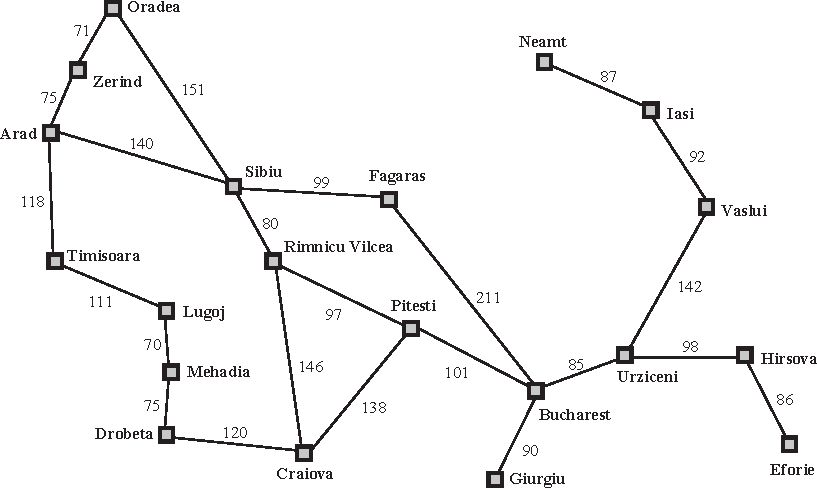
\includegraphics[scale=1]{Romania Map}
\caption{A simplified road map of part of Romania. Numbers are distances.}\label{RomaniaMap}
\end{figure}

\section{Solving problems with agents}
The simplest agents discussed previously were the reflex agents, which base their actions on a direct mapping from states to actions. Such agents cannot operate well in environments for which this mapping would be too large to store and would take too long to learn. Goal-based agents, on the other hand, consider future actions and the desirability of their outcomes.
This chapter describes one kind of goal-based agent called a problem-solving agent.

Our discussion of problem solving begins with precise definitions of problems and their solutions and give several examples to illustrate these definitions. We then describe several general-purpose search algorithms that can be used to solve these problems.

We will see several uninformed search algorithms that are given no information about the problem other than its definition. Although some of these algorithms can solve any solvable problem, none of them can do so efficiently. Informed search algorithms, on the other hand, can do quite well given some guidance on where to look for solutions.
\subsection{Formulation of a problem}
\textbf{Goal formulation}, based on the current situation and the agent’s performance measure, is the first step in problem solving.

\textbf{Problem formulation} is the process of deciding what actions and states to consider, given a goal. We discuss this process in more detail later.

We make several \textcolor{CadetBlue!90}{\textbf{assumption}}: a static, fully accessible, discrete and deterministic environment.Under these assumptions, the \textbf{Solution} to any problem is a fixed sequence of actions.
The process of looking for a sequence of actions that reaches the goal is called \textbf{Search}.
A \textbf{Search Algorithm} takes a problem as input and returns a solution in the form of an action sequence. Once a solution is found, the actions it recommends can be carried out. This is called the \textbf{Execution Phase}.

\subsection{Well-defined problems and solutions}
A problem can be defined formally by five components:
\begin{itemize}
  \item The \textbf{Initial State} that the agent starts in.
  \item A \textbf{description of the possible actions} "a" available to the agent. Given a particular state "s", we say that each of these actions is \textcolor{CadetBlue!90}{\textbf{applicable}} in s.
    ACTIONS(s) returns the set of actions that can be executed in s.
  \item A description of what each action does; the formal name for this is the \textbf{Transition Model}, specified by a function $RESULT(s, a)$ that returns the state that results from doing action a in state s. We also use the term successor to refer to any state reachable from a given state by a single action.
\[RESULT(In(Arad),Go(Zerind)) = In(Zerind)\]
  Together, the Initial State, actions, and transition model implicitly define the \textcolor{CadetBlue!90}{\textbf{State Space}} of the problem the set of all states reachable from the initial state by any sequence of actions. The state space forms a directed network or \textcolor{CadetBlue!90}{\textbf{graph}} in which the \textcolor{CadetBlue!90}{\textbf{nodes}} are states and the \textcolor{CadetBlue!90}{\textbf{links}} between nodes are actions.
  A \textcolor{CadetBlue!90}{\textbf{path}} in the state space is a sequence of states connected by a sequence of actions.
  \item The \textbf{goal test}, which determines whether a given state is a goal state. Sometimes there is an explicit set of possible goal states, and the test simply checks whether the given state is one of them.
  \item A \textbf{path cost function} that assigns a numeric cost to each path. The problem-solving agent chooses a cost function that reflects its own performance measure.
\end{itemize}

%\begin{itemize}
%  \item Initialstate: I am in Timisoara
%  \item Possible actions(action, successor): (go Arad, in Arad), (go Lugoj, in Lugoj)
%  \item Goal test: in Bucarest?
%  \item Path costfrom x to y by the action a: $c(x,a,y)>=0$
%  \item Optimalsolution: the solutionhavingthe lowestcost
%\end{itemize}

\subsection{Search algorithm}

\subsubsection{Search Algorithm structure and the State Space}
A solution is an action sequence, so search algorithms work by considering various possible action sequences.
The possible action sequences starting at the initial state form a search tree with the initial state at the root; the branches are actions and the nodes correspond to states in the state space of the problem.

In this list there are the main components of a state space together with the relation between them:
\begin{itemize}
  \item Path - Path refers to the sequence of nodes along the edges of a tree.

  \item Root - The node at the top of the tree is called root. There is only one root per tree and one path from the root node to any node.

  \item Parent node - Any node except the root node has one edge upward to a node called parent.

  \item Child node - The node below a given node connected by its edge downward is called its child node.

  \item Leaf node - The node which does not have any child node is called the leaf node. Leaf node can be expanded and then become Parent Node if they have children node, or remain Leaf node if they haven't.

  \item Subtree - Subtree represents the descendants of a node.

  \item Visiting - Visiting refers to checking the value of a node when control is on the node.

  \item Traversing - Traversing means passing through nodes in a specific order.

  \item Depth or Levels - Level of a node represents the generation of a node. If the root node is at level 0, then its next child node is at level 1, its grandchild is at level 2, and so on.

  \item Keys - Key represents a value of a node based on which a search operation is to be carried out for a node.

  \item Frontier - The set of all leaf nodes available for expansion at any given point is called the frontier.

  \item Fringe - Collection of nodes generated but not yet expanded
\end{itemize}
\begin{figure}[h!]
\centering
\subfloat[][\emph{Search Tree}]
{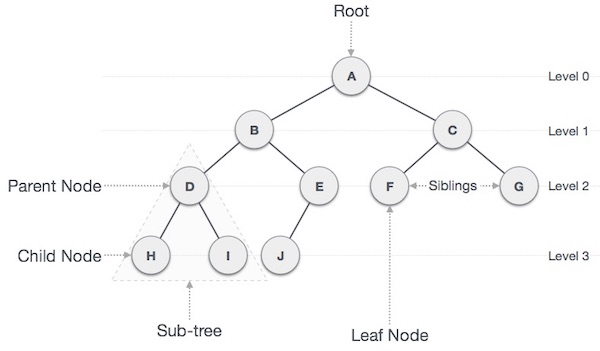
\includegraphics[width=.80\textwidth]{binary_tree.jpg}}
\caption{Search Tree}
\label{fig:Search Tree}
\end{figure}

Search algorithms follows a simple structure:
\begin{enumerate}
  \item The root node of the tree corresponds to the initial state, $In(s=root)$. The first step is to test whether this is a goal state.
  \item Then we need to consider taking various actions:
  We do this by \textbf{expanding} the current state; that is, applying each legal action to the current state, thereby \textbf{generating} a new set of states which are linked by branches to the current (parent node) state leading to new child node.
  \item Now we must apply the specific iterative algorithm that is chosen for the problem and then move to the child node given by the algorithm.
  \item The process of expanding nodes on the frontier continues until either a solution is found or there are no more states to expand.
\end{enumerate}

This is the general \textbf{TREE-SEARCH} algorithm.

Search algorithms all share this basic structure; they vary primarily according to how they choose which state to expand next the so-called \textbf{search strategy}.

An exception is given if there is a repeated state in the search tree such that it can generate a loopy path that can become infinite if we don't take precautions.

The way to avoid exploring redundant paths is to remember where one has been. To do this, we augment the \textbf{TREE-SEARCH} algorithm with a data structure called the \textbf{explored set} (also known as the \textbf{closed list}), which remembers every expanded node. Newly generated nodes that match previously generated nodes ones in the explored set or the frontier can be discarded instead of being added to the frontier. The new algorithm, called \textbf{GRAPH-SEARCH}. The specific algorithms in this chapter draw on this general design.
Clearly, the search tree constructed by the GRAPH-SEARCH algorithm contains at most one copy of each state, so we can think of it as growing a tree directly on the state-space graph. The algorithm has another nice property: the frontier separates the state-space graph into the explored region and the unexplored region, so that every path fromthe initial state to an unexplored state has to pass through a state in the frontier.
\paragraph{Difference between TREE-SEARCH and GRAPH-SEARCH}

Firstly, we have to understand that the underlying problem (or search space) is almost always represented as a graph (although the underlying graph may not contain cycles, so it may represent a tree). So, the difference between tree-search and graph-search is not whether the problem is a tree (a special kind of graph), or a general graph!

The distinction is, instead, how we are traversing the search space (represented as a graph) to search for our goal state and whether we are using an additional list (called the closed list) or not.

So, the basic differences are:
\begin{enumerate}
  \item In the case of a graph search, we use a list, called the closed list (also called explored set), to keep track of the nodes that have already been visited and expanded, so that they are not visited and expanded again.

  \item In the case of a tree search, we do not keep this closed list. Consequently, the same node can be visited multiple (or even infinitely many) times, which means that the produced tree (by the tree search) may contain the same node multiple times.
\end{enumerate}


The advantage of graph search obviously is that, if we finish the search of a node, we will never search it again. On the other hand, the tree search can visit the same node multiple times.

The disadvantage of graph search is that it uses more memory (which we may or may not have) than tree search. This matters because graph search actually has exponential memory requirements in the worst case, making it impractical without either a really good search heuristic or an extremely simple problem.
\subsubsection{Infrastructure for search algorithms Node - Function and Queue}
Search algorithms require a data structure to keep track of the search tree that is being constructed.
For each node n of the tree, we have a structure (usually a class) that contains five components:
\begin{itemize}
  \item n.STATE: the state in the state space to which the node corresponds;
  \item n.PARENT: the node in the search tree that generated this node;
  \item n.ACTION: the action that was applied to the parent to generate the node (n-1,a,n);
  \item n.PATH-COST: the cost, traditionally denoted by $g(n)= \sum_{i=1}^{n} c(i-1, a_{i}, i)$, of the path from the initial state to the node, as indicated by the parent pointers.
\end{itemize}
The function CHILD-NODE takes a parent node and an action
and returns the resulting child node.

These pointers also allow the solution path to be
extracted when a goal node is found; we use the SOLUTION function to return the sequence of actions obtained by following parent pointers back to the root.

Up to now, we have not been very careful to distinguish between nodes and states, but in writing detailed algorithms it’s important to make that distinction. A node is a bookkeeping data structure used to represent the search tree. A state corresponds to a configuration of the world.

Now that we have nodes, we need somewhere to put them. The frontier needs to be stored in such a way that the search algorithm can easily choose the next node to expand QUEUE according to its preferred strategy. The appropriate data structure for this is a queue. The operations on a queue are as follows:
\begin{itemize}
  \item EMPTY?(queue) returns true only if there are no more elements in the queue.
  \item POP(queue) removes the first element of the queue and returns it.
  \item INSERT(element, queue) inserts an element and returns the resulting queue.
\end{itemize}

Queues are characterized by the order in which they store the inserted nodes. Three common variants are the first-in, first-out or FIFO queue, which pops the oldest element of the queue;
the last-in, first-out or LIFO queue (also known as a stack), which pops the newest element of the queue; and the priority queue, which pops the element of the queue with the highest
priority according to some ordering function.

\subsubsection{Problem-Solving performance}
Measuring problem-solving performance before we get into the design of specific search algorithms, we need to consider the criteria that might be used to choose among them.
We can evaluate an algorithm’s performance in four ways:
\begin{itemize}
  \item COMPLETENESS : Is the algorithm guaranteed to find a solution when there is one?
  \item OPTIMALITY: Does the strategy find the optimal solution? An optimal solution has the lowest path cost among all solutions.
  \item TIME COMPLEXITY: How long does it take to find a solution?
  \item SPACE COMPLEXITY: How much memory is needed to perform the search?
\end{itemize}

Time and space complexity are always considered with respect to some measure of the problem difficulty. In theoretical computer science, the typical measure is the size of the state space graph, $|V| + |E|$, where V is the set of vertices (nodes) of the graph and E is the set of edges (links).

This is appropriate when the graph is an explicit data structure that is input to the search program. (The map of Romania is an example of this.)
In AI, the graph is often represented implicitly by the initial state, actions, and transition model and is frequently infinite.
For these reasons, \textcolor{CadetBlue!90}{\textbf{complexity is expressed in terms of three quantities}}: \textbf{b}, the branching factor or maximum number of successors of any node; \textbf{d}, the depth of the shallowest goal node (i.e., the number of steps along the path from the root); and \textbf{m}, the maximum length of any path in the state space. Time is often measured in terms of the number of nodes generated during the search, and space in terms of the maximum number of nodes stored in memory.
For the most part, we describe time and space complexity for search on a tree; for a graph, the answer depends on how “redundant” the paths in the state space are.
To assess the effectiveness of a search algorithm, we can consider just the search cost which typically depends on the time complexity but can also include a term for memory usage or we can use the total cost, which combines the search cost and the path cost of the solution found.

Regarding space complexity: for any kind of graph search, which stores every expanded node in the explored set, the space complexity is always within a factor of b of the time complexity.

\section{Search algorithms}
This section covers several search strategies that come under the heading of \textbf{uninformed search} (also called blind search). The term means that the strategies have no additional information about states beyond that provided in the problem definition. All they can do is generate successors and distinguish a goal state from a non-goal state.
All search strategies are distinguished by the order in which nodes are expanded. Strategies that know whether one non-goal state is “more promising” than another are called \textbf{informed search} or \textbf{heuristic search} strategies.
\subsection{Uninformed Search Algorithms}
\subsubsection{Breadth-first search}
Breadth-first search (ricerca in ampiezza) is a simple strategy in which the root node is expanded first, then all the successors of the root node are expanded next, then their successors, and so on. In general,
all the nodes are expanded at a given depth in the search tree before any nodes at the next level are expanded.

It is complete if the shallowest (più superficiale) goal node is at some finite depth d, breadth-first search will eventually find it after generating all shallower nodes (provided the branching factor b is finite). Note that as soon as a goal node is generated, we know it is the shallowest goal node because all shallower nodes must have been generated already and failed the goal test. Now, the shallowest goal node is not necessarily the optimal one; technically, breadth-first search is optimal if the path cost is a nondecreasing function of the depth of the node. The most common such scenario is that all actions have the same cost.

The root of the search tree generates b nodes at the first level, each of which generates b more nodes, for a total of b 2 at the second level. Each of these generates b more nodes, yielding b 3 nodes at the third level, and so on. Now suppose that the solution is at depth d. In the worst case, it is the last node generated at that level.

Then the total number of nodes generated is
\[b + b^2 + b^3 + \dots + b^d
 = \mathcal{O}(b^d)\]

As for space complexity: for any kind of graph search, which stores every expanded node in the explored set, the space complexity is always within a factor of b of the time complexity. For breadth-first graph search in particular, every node generated remains in memory.
There will be $\mathcal{O}(b^{d-1})$ nodes in the explored set and $\mathcal{O}(b^d)$ nodes in the frontier, so the space complexity is $\mathcal{O}(b^d)$, i.e., it is dominated by the size of the frontier.
 Switching to a tree search would not save much space, and in a state space with many redundant paths, switching could cost a great deal of time.
An exponential complexity bound such as $\mathcal{O}(b^d)$ is scary. It lists, for various values of the solution depth d, the time and memory required for a breadthfirst search with branching factor $b = 10$. The table \textcolor{CadetBlue!90}{\textbf{assumes that 1 million nodes can be generated per second}} and that a node requires $1000$ bytes of storage. Many search problems fit roughly within these assumptions (give or take a factor of $100$) when run on a modern personal computer.
\begin{figure}[h!]
\centering
\subfloat[][\emph{Breadth Search}]
{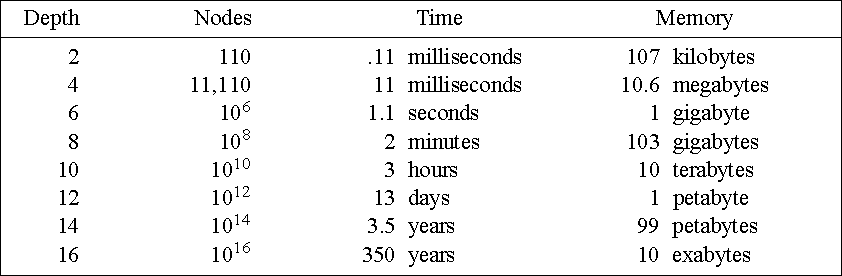
\includegraphics[width=.80\textwidth]{Breadth.pdf}}
\caption{Breadth Search}
\label{fig:Breadth Search}
\end{figure}

\paragraph{General conclusion for uninformed search:}
First, the memory requirements are a bigger problem for breadth-first search than is the execution time.
In general, exponential-complexity search problems
cannot be solved by uninformed methods for any but the smallest instances.
\subsubsection{Uniform-cost search}
When all step costs are equal, breadth-first search is optimal because it always expands the shallowest unexpanded node. By a simple extension, we can find an algorithm that is optimal with any step-cost function. Instead of expanding the shallowest node, uniform-cost search expands the node n with the lowest path cost g(n). This is done by storing the frontier as a priority queue ordered by g.
In addition to the ordering of the queue by path cost, there are two other significant differences from breadth-first search. The first is that the goal test is applied to a node when it is selected for expansion, rather than when it is first generated.
The second difference is that a test is added in case a better path is found to a node currently on the frontier.
It is easy to see that uniform-cost search is optimal in general.
Uniform-cost search does not care about the number of steps a path has, but only about their total cost. Therefore, it will get stuck in an infinite loop if there is a path with an infinite sequence of zero-cost action.

Uniform-cost search is guided by path costs rather than depths, so its complexity is not easily characterized in terms of b and d. Instead, let $C^*$ be the cost of the optimal solution, and assume that every action costs at least $\epsilon$. Then the algorithm’s worst-case time and space complexity is $\mathcal{O}(b^{1+\frac{C^*}{\epsilon}})$.
\subsubsection{Depth-first search}
Depth-first search always expands the deepest node in the current frontier of the search tree.
The search proceeds immediately to the deepest level of the search tree, where the nodes have no successors. As those nodes are expanded, they are dropped from the frontier, so then the search “backs up” to the next deepest node that still has unexplored successors.
Whereas breadth-first-search uses a FIFO queue, depth-first search uses a LIFO queue.
A LIFO queue means that the most recently generated node is chosen for expansion. This must be the deepest unexpanded node because it is one deeper than its parent which, in turn, was the deepest unexpanded node when it was selected.


A variant of depth-first search called backtracking search uses still less memory. In backtracking, only one successor is generated at a time rather than all successors; each partially expanded node remembers which successor to generate next. In this way, only $\mathcal{O}(m)$ memory is needed rather than $\mathcal{O}(bm)$. Backtracking search facilitates yet another memory-saving (and time-saving) trick: the idea of generating a successor by modifying the current state description directly rather than copying it first. This reduces the memory requirements to just one state description and $\mathcal{O}(m)$ actions. For this to work, we must be able to undo each modification when we go back to generate the next successor. For problems with large state descriptions, such as robotic assembly, these techniques are critical to success.

\subsubsection{Depth-limited Search}

The embarrassing failure of depth-first search in infinite state spaces can be alleviated by supplying depth-first search with a predetermined depth limit $\ell$. That is, nodes at depth $\ell$ are  treated as if they have no successors. This approach is called depth-limited search. The depth limit solves the infinite-path problem. Unfortunately, it also introduces an additional source of incompleteness if we choose $\ell < d$, that is, the shallowest goal is beyond the depth limit. (This is likely when d is unknown.) Depth-limited search will also be nonoptimal if we choose $\ell > d$. Its time complexity is $\mathcal{0}(b^{\ell})$ and its space complexity is $\mathcal{O} (b\ell)$.
 Depth-first search can be viewed as a special case of depth-limited search with $\ell=\infty$.

\subsubsection{Iterative Deepening search}
 Iterative Deepening search (or iterative deepening depth-first search) is a general strategy, often used in combination with depth-first tree search, that finds the best depth limit. It does this by gradually increasing the limit first 0, then 1, then 2, and so on—until a goal is found. This will occur when the depth limit reaches d, the depth of the shallowest goal node.

 In general, iterative deepening is the preferred uninformed search method when the search space is large and the depth of the solution is not known.

 \subsubsection{Bidirectional Search}
 The idea behind bidirectional search is to run two simultaneous searches—one forward from the initial state and the other backward from the goal—hoping that the two searches meet in the middle. The motivation is that $b^{d/2} + b^{d/2}$ is much less than $b^d$, or in the figure, the area of the two small circles is less than the area of one big circle centered on the start and reaching to the goal.
Bidirectional search is implemented by replacing the goal test with a check to see whether the frontiers of the two searches intersect; if they do, a solution has been found.
\subsubsection{Comparison}
\begin{figure}[h!t]
\centering
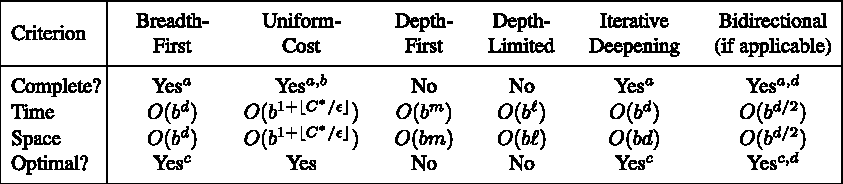
\includegraphics[width=.80\textwidth]{Comparison.pdf}
\caption{ Evaluation of tree-search strategies. $b$ is the branching factor; $d$ is the depth of the shallowest solution; $m$ is the maximum depth of the search tree; $l$ is the depth limit.
Superscript caveats are as follows: $^{a}$ complete if $b$ is finite; $^{b}$ complete if step costs $\geq \epsilon$ for positive $\epsilon$; $^{c}$ optimal if step costs are all identical; $^{d}$ if both directions use breadth-first search.}
\label{fig:Strategies comparison}
\end{figure}

\subsection{Informed search algorithm}
This section shows how an informed \textbf{INFORMED SEARCH} search strategy—one that uses problem-specific knowledge beyond the definition of the problem itself can find solutions more efficiently than can an uninformed strategy.
The general approach we consider is called \textbf{best-first search}. Best-first search is an instance of the general TREE-SEARCH or GRAPH-SEARCH algorithm in which a node is selected for expansion based on an \textbf{evaluation function}, f(n). The evaluation function is construed as a cost estimate, so the node with the lowest evaluation is expanded first. The implementation of best-first graph search is identical to that for uniform-cost search, except for the use of f instead of g to order the priority queue.
The choice of f determines the search strategy. Most best-first algorithms include as a component of f a \textbf{heuristic function}, denoted h(n):

\[h(n) = \text{estimated cost of the cheapest path from the state at node n to a goal state.}\]

(Notice that h(n) takes a node as input, but, unlike g(n), it depends only on the state at that node.)
Heuristic functions are the most common form in which additional knowledge of the problem is imparted to the search algorithm.

For now, we consider them to be arbitrary, non negative, problem-specific functions, with one constraint: \textbf{if n is a goal node, then h(n)=0}. The remainder of this section covers two ways to use heuristic information to guide search.

\subsubsection{Greedy best-first search}
Greedy best-first search tries to expand the node that is closest to the goal, on the grounds that this is likely to lead to a solution quickly. Thus, it evaluates nodes by using just the heuristic function; that is, f(n) = h(n).

We use the \textbf{straight line distance heuristic}, which we will call $h_{SLD}$.

The algorithm is called “greedy”—at each step it tries to get as close to the goal as it can.
Greedy best-first tree search is incomplete even in a finite state space, much like depth-first search and also it is not optimal.
\subsubsection{A\text{*} search: Minimizing the total estimated solution cost}
The most widely known form of best-first search is called A\text{*} (pronounced “A-star search”). It evaluates nodes by combining $g(n)$, the cost to reach the node, and $h(n)$, the cost to get from the node to the goal:
$f(n) = g(n) + h(n)$.
Since $g(n)$ gives the path cost from the start node to node n, and $h(n)$ is the estimated cost of the cheapest path from n to the goal, we have:
\[f(n) = \text{estimated cost of the cheapest solution through n}\]
Thus, if we are trying to find the cheapest solution, a reasonable thing to try first is the node with the lowest value of $g(n) + h(n)$. It turns out that this strategy is more than just reasonable: provided that the heuristic function $h(n)$ satisfies certain conditions, A\text{*} search is both complete and optimal. The algorithm is identical to Uniform-cost search except that A\text{*} uses $g + h$ instead of $g$.

\paragraph{Conditions for optimality: Admissibility and consistency}
The first condition we require for \textbf{optimality} is that h(n) be an admissible heuristic. An admissible heuristic is one that never overestimates the cost to reach the goal. Because g(n) is the actual cost to reach n along the current path, and f(n)=g(n) + h(n), we have as an immediate consequence that f(n) never overestimates the true cost of a solution along the current path through n.
Admissible heuristics are by nature optimistic because they think the cost of solving
the problem is less than it actually is.
An obvious example of an admissible heuristic is the straight-line distance $h_{LSD}$

A second, slightly stronger condition called  \textbf{consistency} (or sometimes monotonicity) is required only for applications of A\text{*} to graph search.
A heuristic h(n) is consistent if, for every node n and every successor n' of n generated by any action a, the estimated cost of reaching the goal from n is no greater than the step cost of getting to n' plus the estimated cost of reaching the goal from n': $h(n) \leq c(n, a, n') + h(n')$.

This is a form of the general \textcolor{CadetBlue!90}{\textbf{triangle inequality}}, which stipulates that each side of a triangle cannot be longer than the sum of the other two sides. Here, the triangle is formed by n, n', and the goal $G_n$ closest to n. For an admissible heuristic, the inequality makes perfect sense:
if there were a route from n to $G_n$ via n' that was cheaper than h(n), that would violate the
property that h(n) is a lower bound on the cost to reach $G_n$.
It is fairly easy to show that \textcolor{CadetBlue!90}{\textbf{every consistent heuristic is also admissible}} as follow from the demonstration:
\[    h(n) \leq c(n, a_{1}, n_{1}) + h(n_{1})\leq  c(n, a_{1}, n_{1}) +  c(n_{1}, a_{2}, n_{2}) + h(n_{2}) \leq \dots\]
\[\dots \leq c(n, a_{1}, n_{1}) + \dots + c(n_{d-1}, a_{d}, G^{*}) + h(G^{*})=C(n,G^{*})\]
Consistency is therefore a stricter requirement than admissibility, but one has to work quite hard to construct heuristics that are admissible but not consistent.
\begin{itemize}
    \item Admissible implies complete
    \item Consistent implies complete and optimal
\end{itemize}
Exercise: Prove that if a heuristic is consistent, it must be admissible. Construct an admissible
heuristic that is not consistent.

\paragraph{Optimality of A*}
As we mentioned earlier, A* has the following properties: the tree-search version of A\text{*} is
optimal if $h(n)$ is admissible, while the graph-search version is optimal if $h(n)$ is consistent.
We show the second of these two claims since it is more useful. The argument essentially mirrors the argument for the optimality of uniform-cost search, with g replaced by f just as in the A\text{*} algorithm itself.
The first step is to establish the following: if h(n) is consistent, then the values of f(n) along any path are nondecreasing. The proof follows directly from the definition of consistency. Suppose n' is a successor of n; then $g(n')=g(n) + c(n, a, n')$ for some action a, and we have 
\begin{equation}
    f(n') = g(n') + h(n') = g(n) + c(n, a, n') + h(n') \geq g(n) + h(n) = f(n)
\end{equation}

The next step is to prove that whenever A\text{*} selects a node n for expansion, the optimal path to that node has been found. Were this not the case, there would have to be another frontier node n' on the optimal path from the start node to n, because f is nondecreasing along any path, n' would have lower f-cost than n and would have been selected first.
Because f is nondecreasing along any path, n' would have lower f-cost than n and would have been selected first.\footnote{See figure 3.9 pag. 78 \cite{RusselNorvig:2009dg} for the separation properties of graph}


\paragraph{Inventing Heuristic function}
code: 8-puzzle game\\

Queen game\\

see crystal quest, a game for machintosh using greedy algorithm in the demo mode

\paragraph{The effect of heuristic accuracy on performance}
One way to characterize the quality of a heuristic is the effective \textcolor{CadetBlue!90}{\textbf{branching factor}} \textbf{b\text{*}}. If the total number of nodes generated by A\text{*} for a particular problem is N and the solution depth is d, then b\text{*} is the branching factor that a uniform tree of depth d would have to have in order to contain $N + 1$ nodes. Thus, $N + 1 = 1+b\text{*} + (b\text{*})^{2} +\dots+ (b\text{*})^d$.
For example, if A\text{*} finds a solution at depth 5 using 52 nodes, then the effective branching factor is 1.92. The effective branching factor can vary across problem instances, but usually it is fairly constant for sufficiently hard problems. (The existence of an effective branching factor follows from the result, mentioned earlier, that the number of nodes expanded by A\text{*} grows exponentially with solution depth.) Therefore, experimental measurements of b* on a small set of problems can provide a good guide to the heuristic’s overall usefulness. A welldesigned heuristic would have a value of b\text{*} close to 1, allowing fairly large problems to be solved at reasonable computational cost.

\paragraph{Learning heuristics from experience}
Hints on generating a heuristic function using neural network.

\section{Local Search}
In the last Section we addressed a single category of problems: observable, deterministic, known environments where the solution is a sequence of actions. In this chapter, we look at what happens when these \textcolor{CadetBlue!90}{\textbf{assumptions are relaxed}}.
The answer to this problem is given by \textbf{local search} in the state space, evaluating and modifying one or more current states rather than systematically exploring paths from an initial state.
These algorithms are suitable for problems in which all that matters is the solution state, not the path cost to reach it. The family of local search algorithms includes methods inspired by statistical physics (\textbf{simulated annealing}) and evolutionary biology (\textbf{genetic algorithms}).

Then, we examine what happens when we relax the assumptions of determinism and observability. The key idea is that if an agent cannot predict exactly what percept it will receive, then it will need to consider what to do under each contingency that its percepts may reveal. With partial observability, the agent will also need to keep track of the states it might be in.
\paragraph{Local search:}
The search algorithms that we have seen so far are designed to explore search spaces systematically.
This systematicity is achieved by keeping one or more paths in memory and by recording which alternatives have been explored at each point along the path.
In many problems, however, the path to the goal is irrelevant. For example, in the 8-queens problem, what matters is the final configuration of queens, not the order in which they are added. 

If the path to the goal does not matter, we might consider a different class of algorithms, ones that do not worry about paths at all. Local search algorithms operate using a single \textbf{current node} (rather than multiple paths) and generally move only to neighbors of that node. Typically, the paths followed by the search are not retained.
Although local search algorithms are not systematic, they have two key advantages: 
\begin{enumerate}
    \item they use very little memory—usually a constant amount;
    \item they can often find reasonable solutions in large or infinite (continuous) state spaces for which systematic algorithms are unsuitable.
\end{enumerate}
In addition to finding goals, local search algorithms are useful for solving \textbf{pure optimization problems}, in which the aim is to find the best state according to an \textbf{objective function}. Many optimization problems do not fit the “standard” search model introduced. 
For example, nature provides an objective function that Darwinian evolution could be seen as attempting to optimize, but there is no “goal test” and no “path cost” for this problem.
To understand local search, we find it useful to consider the state-space landscape. A landscape has both “location” (defined by the state) and “elevation” (defined by the value of the heuristic cost function or objective function). If elevation corresponds to \textbf{GLOBAL MINIMUM} cost, then the aim is to find the lowest valley: a global minimum; if elevation corresponds \textbf{GLOBAL MAXIMUM} to an objective function, then the aim is to find the highest peak—a global maximum. (You can convert from one to the other just by inserting a minus sign.) Local search algorithms explore this landscape. A \textbf{complete} local search algorithm always finds a goal if one exists;an \textbf{optimal} algorithm always finds a global minimum/maximum.

\begin{figure}[h!t]
\centering
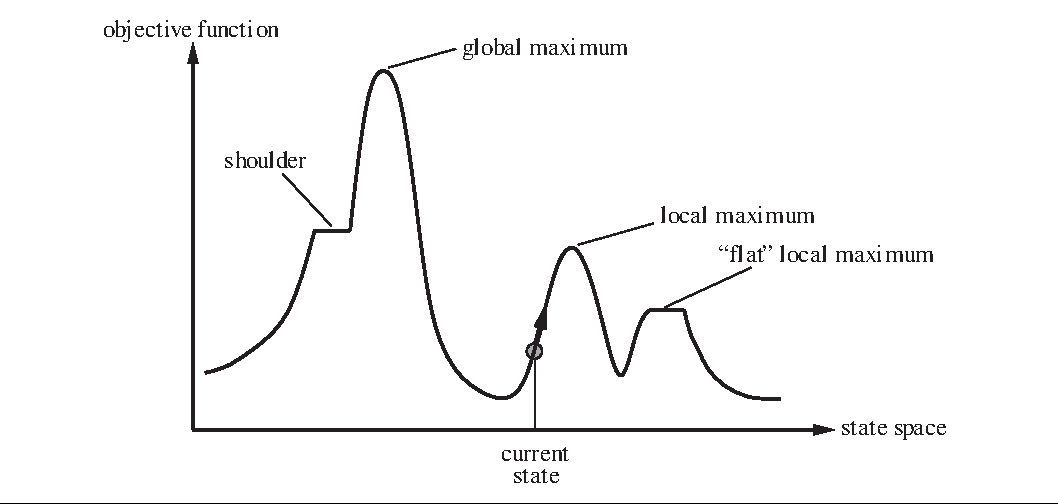
\includegraphics[scale=0.8]{Maxmin.pdf}
\caption{A one-dimensional state-space landscape in which elevation corresponds to the
objective function. The aim is to find the global maximum. Hill-climbing search modifies
the current state to try to improve it, as shown by the arrow. The various topographic features
are defined in the text.}
\end{figure}

\subsection{Strategies for local search}
\begin{itemize}
    \item Hill-climbing search 
    \item Montecarlo technique, simulated annealing: random walk and down-hill moves
    \item Local beam search: generates all successors of k replica, then selects the best k successors from the complete list
    \item Stochastic beam search: chooses randomly k successors from the complete list, with probability increasing with its value
    \item Genetic algorithms: combines two parents and tries to mimic natural selection
\end{itemize}
\subsection{Hill-climbing search or Greedy local search}
It is simply a loop that continually moves in the direction of increasing value—that is, uphill. It
terminates when it reaches a “peak” where no neighbor has a higher value. The algorithm
does not maintain a search tree, so the data structure for the current node need only record
the state and the value of the objective function. Hill climbing does not look ahead beyond
the immediate neighbors of the current state. This resembles trying to find the top of Mount
Everest in a thick fog while suffering from amnesia.
To illustrate hill climbing, we will use the 8-queens problem.
Local search algorithms typically use a complete-state formulation: each state contain all the configuration of the system. Hill climbing is sometimes called greedy local search because it grabs a good neighbor state without thinking ahead about where to go next. Although greed is considered one of the seven deadly sins, it turns out that greedy algorithms often perform quite well.
\\
Unfortunately, hill climbing often gets stuck for the following reasons:
\begin{itemize}
\item Local maximum: a local maximum is a peak that is higher than each of its neighboring
states but lower than the global maximum. Hill-climbing algorithms that reach the
vicinity of a local maximum will be drawn upward toward the peak but will then be
stuck with nowhere else to go.
\item Ridges: a ridge is shown in Figure \ref{ridges}. Ridges result in a sequence of local maxima
that is very difficult for greedy algorithms to navigate.
\item Plateaux: a plateau is a flat area of the state-space landscape. It can be a flat local maximum, from which no uphill exit exists, or a shoulder, from which progress is possible. A hill-climbing search might get lost on the plateau.
\end{itemize}
In each case, the algorithm reaches a point at which no progress is being made.
The algorithm may reaches a plateau where the best successor has the same value as the current state. Might it not be a good idea to keep going—to allow a
sideways move in the hope that the plateau is really a shoulder? The answer is usually yes, but we must take care. If we always allow sideways moves when there are no uphill moves, an infinite loop will occur whenever the algorithm reaches a flat local maximum that is not a shoulder. One common solution is to put a limit on the number of consecutive sideways moves allowed.
Many variants of hill climbing have been invented.
\begin{figure}[h!t]
\centering
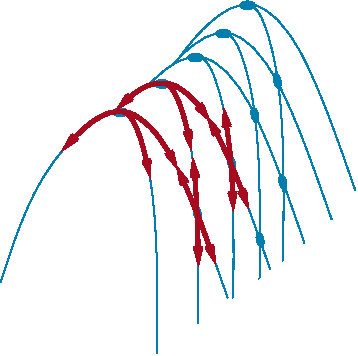
\includegraphics[scale=0.8]{Ridges.pdf}
\caption{Illustration of why ridges cause difficulties for hill climbing. The grid of states
(dark circles) is superimposed on a ridge rising from left to right, creating a sequence of local
maxima that are not directly connected to each other. From each local maximum, all the
available actions point downhill.}\label{ridges}
\end{figure}

\paragraph{Random-restart hill climbing} is a variant of the technique. 
It conducts a series of hill-climbing searches from randomly generated initial states, until a goal is found. It is trivially complete with probability approaching 1, because it will eventually generate a goal state as the initial state. If each hill-climbing search has a probability p of success, then the expected number of restarts required is 1/p.

\subsection{Simulated Annealing}
A hill-climbing algorithm that never makes “downhill” moves toward states with lower value (or higher cost) is guaranteed to be incomplete, because it can get stuck on a local maximum.
In contrast, a purely random walk—that is, moving to a successor chosen uniformly at random from the set of successors—is complete but extremely inefficient. Therefore, it seems reasonable to try to combine hill climbing with a random walk in some way that yields
both efficiency and completeness.
\textbf{Simulated annealing} is such an algorithm. In metallurgy, \textbf{annealing} is the process used to temper or harden metals and glass by heating them to a high temperature and then gradually cooling them, thus allowing the material to reach a low energy crystalline state. To explain simulated annealing, we switch our point of view from hill climbing to \textbf{gradient descent} and imagine the task of getting a ping-pong ball into the deepest crevice in a bumpy surface. If we just let the ball roll, it will come to rest at a local minimum. If we shake the surface, we can bounce the ball out of the local minimum. The trick is to shake just hard enough to bounce the ball out of local minima but not hard enough to dislodge it from the global minimum. The simulated-annealing solution is to start by shaking hard (i.e., at a high temperature) and then gradually reduce the intensity of the shaking (i.e., lower the temperature).
The innermost loop of the simulated-annealing algorithm is quite similar to hill climbing. Instead of picking the best move, however, it picks a random move. If the move
improves the situation, it is always accepted. Otherwise, the algorithm accepts the move with some probability less than 1. The probability decreases exponentially with the “badness” of the move—the amount $\Delta E$ by which the evaluation is worsened.
The probability also decreases as the “temperature” T goes down: “bad” moves are more likely to be allowed at the start when T is high, and they become more unlikely as T decreases. If the schedule lowers T slowly enough, the algorithm will find a global optimum with probability approaching 1.

\subsubsection{Solving again Travelling Salesman DA COMPLETARE MATIAS}
Pag. 549 Numerical Recipes Approfondire.
Pag 551 Traveling Salesman

\subsection{Local Beam Search}
Keeping just one node in memory might seem to be an extreme reaction to the problem of
memory limitations. The local beam search algorithm\footnote{Local beam search is an adaptation of \textbf{beam search}, which is a path-based algorithm.} keeps track of k states rather than just one. It begins with k randomly generated states. At each step, all the successors of all k states are generated. If any one is a goal, the algorithm halts. Otherwise, it selects the k best successors from the complete list and repeats.
At first sight, a local beam search with k states might seem to be nothing more than running k random restarts in parallel instead of in sequence. In fact, the two algorithms are quite different. In a random-restart search, each search process runs independently of the others. In a local beam search, useful information is passed among the parallel search threads. In effect, the states that generate the best successors say to the others, “Come over here, the grass is greener!” The algorithm quickly abandons unfruitful searches and moves its resources to where the most progress is being made. In its simplest form, local beam search can suffer from a lack of diversity among the k states—they can quickly become concentrated in a small region of the state space, making the search little more than an expensive version of hill climbing. 

A variant called \textbf{stochastic beam search}, analogous to stochastic hill climbing, helps alleviate this problem. Instead of choosing the best k from the the pool of candidate successors, stochastic beam search chooses k successors at random, with the probability of choosing a given successor being an increasing function of its value. Stochastic beam search bears some resemblance to the process of natural selection, whereby the “successors” (offspring) of a “state” (organism) populate the next generation according to its “value” (fitness).


\subsection{Genetic algorithm}
A \textbf{genetic algorithm} (or GA) is a variant of stochastic beam search in which successor states are generated by combining two parent states rather than by modifying a single state. The analogy to natural selection is the same as in stochastic beam search, except that now we are dealing with sexual rather than asexual reproduction.
Like beam searches, GAs begin with a set of k randomly generated states, called the \textbf{population}. Each state, or \textbf{individual}, is represented as a string over a finite alphabet—most commonly, a string of 0s and 1s. For example, an 8-queens state must specify the positions of 8 queens, each in a column of 8 squares, and so requires $8\times \log{2 8}=24$ bits. Alternatively, the state could be represented as 8 digits, each in the range from 1 to 8.
\begin{figure}[h!]
\centering
{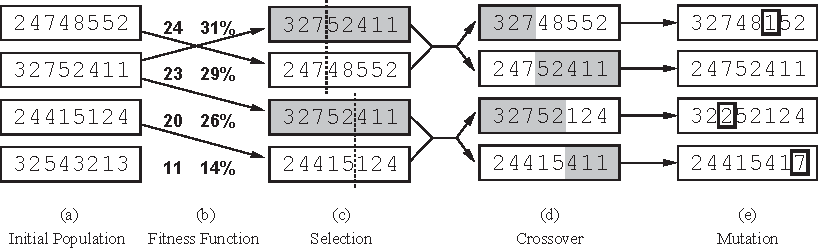
\includegraphics[width=.80\textwidth]{Genetic Algorithm (1).pdf}}
\caption{}
\label{fig:geneticalgorithm1}
\end{figure}

\begin{figure}[h!]
\centering
{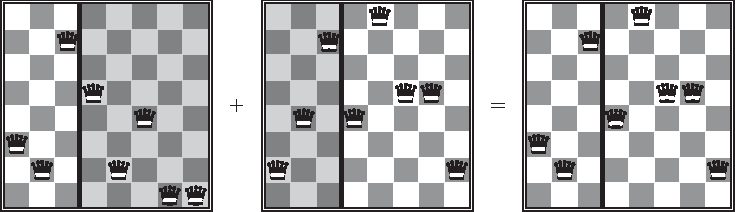
\includegraphics[width=.80\textwidth]{Genetic Algorithm (2).pdf}}
\caption{}
\label{fig:geneticalgorithm2}
\end{figure}
The production of the next generation of states is shown in Figure \ref{fig:geneticalgorithm1}(b)–(e). In (b), each state is rated by the objective function, or (in GA terminology) the \textbf{fitness function}. A fitness function should return higher values for better states, so, for the 8-queens problem we use the number of non-attacking pairs of queens, which has a value of 28 for a solution.
The values of the four states are 24, 23, 20, and 11. In this particular variant of the genetic algorithm, the probability of being chosen for reproducing is directly proportional to the fitness score, and the percentages are shown next to the raw scores.
In (c), two pairs are selected at random for reproduction, in accordance with the probabilities in (b). Notice that one individual is selected twice and one not at all\footnote{There are many variants of this selection rule. The method of culling, in which all individuals below a given threshold are discarded, can be shown to converge faster than the random version}. 
For each pair to be mated, a \textbf{crossover} point is chosen randomly from the positions in the string. In Figure \ref{fig:geneticalgorithm1}, the crossover points are after the third digit in the first pair and after the fifth digit in the second pair.

In (d), the offspring themselves are created by crossing over the parent strings at the crossover point. For example, the first child of the first pair gets the first three digits from the first parent and the remaining digits from the second parent, whereas the second child gets the first three digits from the second parent and the rest from the first parent. The 8-queens states involved in this reproduction step are shown in Figure \ref{fig:geneticalgorithm2}. The example shows that when two parent states are quite different, the crossover operation can produce a state that is a long way from either parent state. It is often the case that the population is quite diverse early on in the process, so crossover (like simulated annealing) frequently takes large steps in the state space early in the search process and smaller steps later on when most individuals are quite similar.

Finally, in (e), each location is subject to random \textbf{mutation} with a small independent probability. One digit was mutated in the first, third, and fourth offspring. In the 8-queens problem, this corresponds to choosing a queen at random and moving it to a random square in its column.

Like stochastic beam search, genetic algorithms combine an uphill tendency with random exploration and exchange of information among parallel search threads.
The primary advantage, if any, of genetic algorithms comes from the crossover operation. Yet it can be shown mathematically that, if the positions of the genetic code are permuted initially in a random order, crossover conveys no advantage. Intuitively, the advantage comes from the ability of crossover to combine large blocks of letters that have evolved independently to perform useful functions, thus raising the level of granularity at which the search operates. For example, it could be that putting the first three queens in positions 2, 4, and 6 (where they do not attack each other) constitutes a useful block that can be combined with other blocks to construct a solution. 
The theory of genetic algorithms explains how this works using the idea of a \textbf{schema}, which is a substring in which some of the positions can be left unspecified. For example, the schema 246***** describes all 8-queens states in which the first three queens are in positions 2, 4, and 6, respectively. Strings that match the schema (such as 24613578) are called \textbf{instances} of the schema.

In practice, genetic algorithms have had a widespread impact on optimization problems, such as circuit layout and job-shop scheduling.
\subsubsection{GA application (DA FARE)}
pip install geneticalgorithm
\\
1. Cap 4.1.4 \cite{RusselNorvig:2009dg}\\
2. Traveling salesman from\\ \url{https://towardsdatascience.com/evolution-of-a-salesman-a-complete-genetic-algorithm-tutorial-for-python-6fe5d2b3ca35}\\
3. Animating genetic algorithm for traveling salesman \url{https://towardsdatascience.com/animating-the-traveling-salesman-problem-56da20b95b2f}\\
4. Reminder of classes in python
\chapter{Monte Carlo techniques}\label{chap:2}


\section{Mothecarlo Technique DA COMPLETARE MATIAS}

\subsection{Random Number}
With hindsight, it seems clear that the whole field of random number generation
was mesmerized, for far too long, by the simple recurrence equation:
\begin{equation}
I_{i+1} = aI_{i} + b \pmod{m}
\label{eq:1}
\end{equation}


Here m is called the modulus, a is a positive integer called the multiplier, and c
(which may be zero) is nonnegative integer called the increment. For c different from 0, the equation is called a linear congruential generator (LCG). When c is equal to 0, it is sometimes
called a multiplicative LCG or MLCG.
The recurrence \ref{eq:1} must eventually repeat itself, with a period that is obviously no greater than m. If m; a; and c are properly chosen, then the period will be
of maximal length, i.e., of length m. In that case, all possible integers between 0 and
$m-1$ occur at some point, so any initial “seed” choice of I 0 is as good as any other:
The sequence just takes off from that point, and successive values I j are the returned
“random” values.
But there is a problem with the number obtained trough this procedure;if k random numbers at a time are used to plot points in k-dimensional space (with each coordinate between 0 and 1), then the points will not
tend to “fill up” the k-dimensional space, but rather will lie on $k-1$ dimensional
“planes”. There will be at most about $m^{1/k}$ such planes.If the constants m and a
are not very carefully chosen, there will be many fewer than that (for this reason this way is not used with Monte Carlo technique). The number m
was usually close to the machine’s largest representable integer, often $2^{32}$
(see pg345)
\begin{figure}[h!t]
\centering
\begin{subfigure}[ht]{0.45\textwidth}
	\centering
	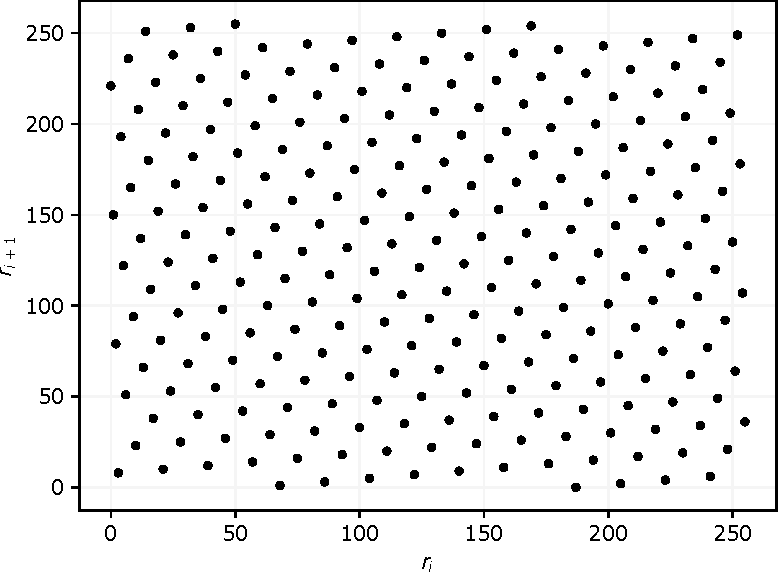
\includegraphics[width=\textwidth]{LCG}
	\caption{}\label{SpectralMethod2d}
\end{subfigure}
\hfill
\begin{subfigure}[ht]{0.51\textwidth}
	\centering
	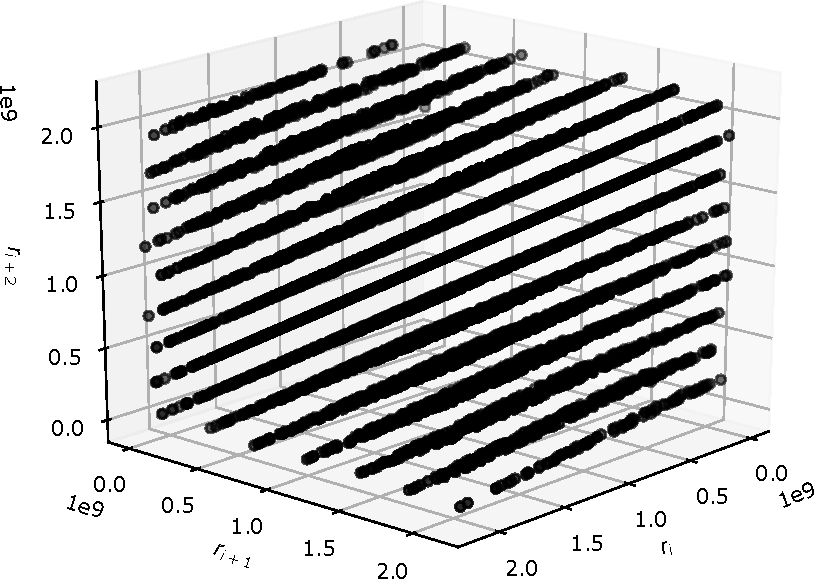
\includegraphics[width=\textwidth]{RANDU}
        \caption{}\label{SpectralMethod3d}
\end{subfigure}
\caption{\attachfile[icon=CustomPushPin,modified=20210303134907+01'00',size=377574]{Attachments/Spectral Test.ipynb} Examples of 2D (a) and 3D (b) spectral methods: (a) is set with $m=256$, $a=137$, $b=187$ (these parameters give full period), while (b) has $m=2^{31}$, $a=65539$, $b=0$ (this congruential generator is the (in)famous \texttt{RANDU}).}\label{SpectralMethod}
\end{figure}
\subsubsection{Ran0: the minimal standard}
NB di questa parte dobbiamo ancora prendere i riferimenti corretti

\subsection{Deviates from other distributions (from pg 361 num rec)}
Before, we learned how to generate random deviates with a uniform probability
between 0 and 1, denoted $U(0,1)$.
The probability of generating a number between
$x$ and $x+dx$ is
\[p(x)dx = \begin{cases}dx & 0 \le x < 1 \\ 0 & otherwise \end{cases}\]
Now we want generate random deviates drawn from other
probability distributions

\subsection{Exponential Deviates}
Suppose that we generate a uniform deviate $x$ and then take some prescribed
function of it, $y(x)$. The probability distribution of $y$, denoted $p(y)dy$, is determined
by the fundamental transformation law of probabilities, which is simply:
\[\left | p(y)dy \right |= \left | p(x)dx \right |\]
or 
\[\left | p(y)\right |= \left | p(x)\right | \left | \frac{dx}{dy} \right |\]
As example, take $y(x) = -\ln(x)$
We obtain:
\[\left | p(y)dy \right | = \left | \frac{dx}{dy} \right |dy = e^{-y}dy\]
NB $f^{-1}$ in this case is $x=e^{-y}$

I want number distributed as $e^{-y}$, so i generate random number (I know how do it), i take the $-\ln(x)$ of this number and what i obtain are numbers distributed exponentially. 

This distribution occurs frequently in real life, usually as the distribution of waiting times between independent Poisson-random events, for example the radioactive decay of nuclei.

\subsubsection{Transformation Method}
Best formalism can be found at:

\emph{\url{https://en.wikipedia.org/wiki/Inverse_transform_sampling}}


Let’s see what is involved in using the above transformation method to generate some arbitrary desired distribution of y’s, say one with $p(y)=f(y)$ for some positive function $f$ whose integral is 1. According to:
\[\left | p(y)\right |= \left | p(x)\right | \left | \frac{dx}{dy} \right |\]
we have to solve the equation:
\[ \frac{dx}{dy} = f(y) \]
but the solution of this equation is just $x=F(y)$ where $F(y)$ is the integral of $f(y)$. The desired transformation that takes a uniform deviate into one distributed as $f(y)$ is therefore: 
\[ y(x)=F^{-1}(x) \]
Since $F(y)$ is the area under the probability curve to the left of y, is just the prescription:
Choose a uniform random x, then find the value y that has that fraction x of probability area to its left, and return the value y.

\begin{figure}[h!t]
\centering
%\subfloat[][\emph{}]
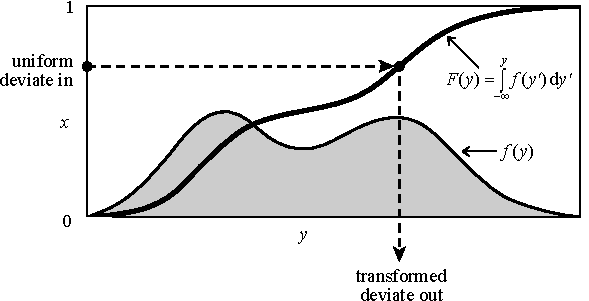
\includegraphics[scale=1]{Transformation Method}
\caption{Transformation method for generating a random deviate y from a known probability distribution $p(y)$. The indefinite integral of $p(y)$ must be known and invertible. A uniform deviate x is chosen between 0 and 1. Its corresponding y on the definite-integral curve is the desired deviate.}\label{fig:Transformation method}
\end{figure}

\subsection{Rejection Method}
The rejection method is a powerful, general technique for generating random deviates whose distribution function $p(x)dx$ (probability of a value occurring between x and $x+dx$) is known and computable.The rejection method does not require that the cumulative distribution function (indefinite integral of $p(x)$) be readily computable, much less the inverse of that function — which was required for the transformation method in the previous section.
The rejection method is based on a simple geometrical argument.

\begin{figure}[h!t]
\centering
\subfloat[][\emph{Rejection method for generating a random deviate x from a known probability distribution $p(x)$ that is everywhere less than some other function $p(x)$.The transformation method is first used to generate a random deviate x of the distribution f. A second uniform deviate is used to decide whether to accept or reject that x. If it is rejected, a new deviate of f is found, and so on.
The ratio of accepted to rejected points is the ratio of the area under p to the area between p and f}]
{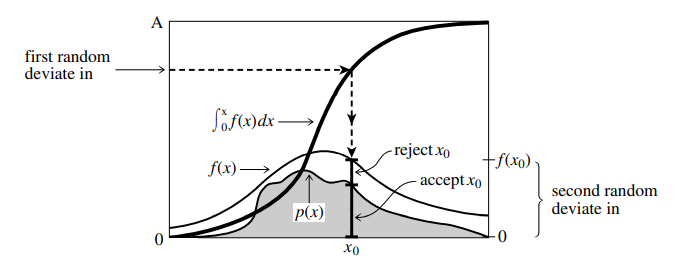
\includegraphics[width=.80\textwidth]{Rejection Method.PNG}}
\caption{}
\label{fig:Rejection method}
\end{figure}

Draw a graph of the probability distribution $p(x)$ that you wish to generate, so that the area under the curve in any range of x corresponds to the desired probability of generating an x in that range. If we had some way of choosing a random point in two dimensions, with uniform probability in the area under your curve, then the x value of that random point would have the desired distribution.

Now, on the same graph, draw any other curve f(x) that has finite (not infinite) area and lies everywhere above your original probability distribution. (This is always possible, because your original curve encloses only unit area, by definition of probability).We will call this $f(x)$ the \textbf{comparison function} . Imagine now that you have some way of choosing a random point in two dimensions that is uniform in the area under the comparison function. Whenever that point lies outside the area under the original probability distribution, we will reject it and choose another random point.
Whenever it lies inside the area under the original probability distribution, we will accept it.

\textbf{It should be obvious that the accepted points are uniform in the accepted area, so that their x values have the desired distribution.} It should also be obvious that the fraction of points rejected just depends on the ratio of the area of the comparison function to the area of the probability distribution function, not on the details of shape of either function.

It remains only to suggest how to choose a uniform random point in two dimensions under the comparison function $f(x)$. It is used a variant of the transformation method,\textbf{ be sure to have chosen a comparison function whose indefinite integral is known analytically, and is also analytically invertible to give x as a function of “area under the comparison function to the left of x.”} Now pick a uniform deviate between 0 and A, where A is the total area under $f(x)$, and use it to get a corresponding x.
Then pick a uniform deviate between 0 and $f(x)$ as the y value for the two-dimensional point. Finally, accept or reject according to whether it is respectively less than or greater than $p(x)$.

\subsection{Special Technique for Gaussian Distribution-Prof.}
Consider an ideal gas (compose by N), with whatever initial distribution of velocities. If the molecule can interact each other after a time interval $\Delta t$ they thermalized (they reach the thermodynamic equilibrium, so the distribution of the velocities is given by the Maxwell Boltzmann distribution: 
\[p(x) = \exp{\left(\frac{-E}{k_{\text{B}}T}\right)} = \exp{\left(\frac{-mv^2}{2k_{\text{B}}T}\right)}\]
This is the idea beyond this technique, we star from whatever distribution $f(x)$, and randomly pick up 2 particle ($j$ and $i$) from the gas (2 point in the interval and evaluate M.B.), then compute:
\[ v_{j}' = \frac{v_{j} + v_{i}}{\sqrt{2}} \]
\[ v_{i}' = \frac{v_{j} - v_{i}}{\sqrt{2}} \]

Now $v_{i}'$ and $v_{j}'$ are the \textbf{new velocities} of the particle $i$ and $j$, if you repeat the procedure a few time I'll end up with a Gaussian distribution (Maxwell Boltzmann in function of velocities)
if I have N particles the number of collision needed to thermalized is the order of $3N$ (so I have to repeat this procedure $3N$ times in a way of produce $N$ number distributed in a Gaussian Way).


\subsection{Metropolis Algorithm - Proof} 
The Metropolis algorithm is a general technique that allows to generate random number distributed according to a certain density probability $P(x)$ (it works even in more than 1 dimension). The Metropolis algorithm is based in few steps:

\newcounter{elenco}
\setcounter{elenco}{0}
\begin{list}{\stepcounter{elenco}\arabic{elenco}}{\setlength{\itemsep}{0.5cm}}
\item Generate a random number $x_n$.
\item Generate a new number $x_1$ through: $x_{n+1} = x_n + r \Delta$ where $r$ is a random number between $-1$ and $1$ and $\Delta$ is the typical scale on which the function $P(x)$ is changing (for example for a Gaussian is the variance).
N.B. $\Delta$ is the only information that we must have about the function $P(x)$. 
\item if $ f(x_{n+1}) > f(x_{n}) $ we always keep the point $x_{n+1}$\\
    if $ f(x_{n+1}) < f(x_{n}) $, compute the ratio $ R = \frac{f(x_{n+1})}{f(x_n)} $ of course $R \in \left[ 0,1 \right]$, now generate another pseudo random number $r' \in \left[ 0,1 \right]$, compare $R$ with $r'$  and if $ r'< R$ we keep $ x_{n+1} $ otherwise we reject $x_{n+1}$
\end{list}

We want show that if we repeat this procedure many times at the end the distribution of the points will reach an equilibrium an that this equilibrium correspond to the function P(x) .Now suppose that we have already generated $N$ points and we are moving them with the previous procedure and that $f(x)$ is a function proportional to $P(x)$. If we made a partition of the interval (in which in defined the function n) we can count the number of points in each interval (bin), so if $n_i$ are the points in the bin $i$, the variation of the number of point is $ \Delta n_i = n_j P_{ji} - n_i P_{ij}$ where $P_{ji}$ is the probability for a point in the bin $j$ to go in the bin $i$ and $P_{ij}$ is the probability for a point in the bin $i$ to go in the bin $j$. So we have: 
\[\Delta n_i = n_j P_{ij} \frac{P_{ji}}{P_{ij}} - \frac{n_i}{n_j}\]
\[ if \hspace{10pt} \frac{n_i}{n_j} > \frac{P_{ji}}{P_{ij}} \to \Delta n_i < 0 \]
Hence the system is evolving in a way that if we have too much points in $i$ the $\Delta n_i$ is negative (we are removing points from the bin $i$) and vice versa; so in this way a sort of equilibrium will be reach.
The probability $P_ij$ can be write as the product of 2 number, $ P_{ij} = g_{ij} A_{ij } $ where $g_{ij}$ is the probability that being in $i$ we generate a point in $i$ (we assume that $ g_{ij} = g_{ji} $) and $A_{ij}$ is the acceptance probability $A_{ij} = min \left\{1, \frac{f_j}{f_i} \right\}$ (so if $\frac{f_j}{f_i} > 1$ $A_{ij}$ is equal to one hence we always keep the new point compatible with what we said above), so from that we get:

\[ if \hspace{10pt} \frac{f_j}{f_i} < 1 \hspace{10pt} then \hspace{10pt}  A_{ij} = \frac{f_j}{f_i} \hspace{10pt} and \hspace{10pt} A_{ji} = 1 \hspace{10pt}\to \hspace{10pt} \frac{A_{ji}}{A_{ij}} = \frac{f_i}{f_j} \]
\[ if \hspace{10pt} \frac{f_j}{f_i} > 1 \hspace{10pt} then \hspace{10pt} A_{ij} = 1 \hspace{10pt} and \hspace{10pt} A_{ji} = \frac{f_i}{f_j} \hspace{10pt} \to \hspace{10pt} \frac{A_{ji}}{A_{ij}} = \frac{f_i}{f_j} \]

and finally,

\[ \frac{p_{ji}}{p_{ij}} = \frac{A_{ji}}{A_{ij}} = \frac{f_i}{f_j} \to \frac{n_i}{n_j} = \frac{f_i}{f_j} \]

therefore we are generating points according the function $f(x)$.

Code: Area of the circle, IdealGas-MarkovChain.  

\subsection{Simulated annealing}
\textit{The method of simulated annealing} is a technique that has attracted significant attention as suitable for optimization problems of large scale, especially ones where a desired global extremum is hidden among many poorer, local extrema. For practical purposes, simulated annealing has effectively “solved” the famous traveling salesman problem of finding the shortest cyclical itinerary for a traveling salesman who must visit each of N cities in turn and the problem of the arrangement of several hundred thousand circuit elements on a tiny silicon substrate is optimized so as to minimize interference among their connecting wires.
Notice that the two applications cited are both examples of combinatorial minimization. There is an objective function to be minimized, as usual, but the space over which that function is defined is not simply the N-dimensional space of $N$ continuously variable parameters. Rather, it is a discrete, but very large, configuration space, like the set of possible orders of cities, or the set of possible allocations of silicon "real estate” blocks to circuit elements.
At the heart of the method of simulated annealing is an analogy with thermodynamics, specifically with the way that liquids freeze and crystallize or metals cool and anneal. At high temperatures, the molecules of a liquid move freely with respect to one another. If the liquid is cooled slowly, thermal mobility is lost. The atoms are often able to line themselves up and form a pure crystal that is completely ordered over a distance up to billions of times the size of an individual atom in all directions. This crystal is the state of minimum energy for this system. The amazing fact is that, for slowly cooled systems, nature is able to find this minimum energy state. In fact, if a liquid metal is cooled quickly or “quenched,” it does not reach this state but rather ends up in a polycrystalline or amorphous state having somewhat higher energy.
 The so-called Boltzmann probability distribution,
 \[ P(E) \sim \exp(-E/KT) \]
expresses the idea that a system in thermal equilibrium at temperature T has its energy probabilistically distributed among all different energy states E. Even at low temperature, there is a chance, albeit a very small one, of a system being in a high energy state. Therefore, there is a corresponding chance for the system to get out of a local energy minimum in favor of finding a better, more global one. In other words, the system sometimes goes uphill as well as downhill; but the lower the temperature, the less likely is any significant uphill excursion.
N.B The crutial idea is that \textit{to minimize E means to maximize $P(E)$}

Code: Simulated-Annealing.

Pag. 825 Numerical Recipes 
Simulated Annealing pag 549 Numerical recipes: way to use a global minimum in triky situation, without getting stuck.

\subsubsection{Traveling Salesman with Metropolis}

%\newcounter{elenco}
%\setcounter{elenco}{0}
%\begin{list}{\stepcounter{elenco}\arabic{elenco}}{\setlength{\itemsep}{0.5cm}}
\begin{enumerate}
\item \textit{Configuration.} The cities are numbered $i = 1,\dots,N$ and each has coordinates $(x_i,y_i)$. A configuration is a permutation of the number $1,\dots,N$, interpreted as the order in which the cities are visited.
\item \textit{Rearrangements.} An efficient set of moves has been suggested by Lin, (Lin, S. 1965, “Computer Solutions of the Traveling Salesman Problem,” Bell System Technical Journal, vol. 44, pp. 2245–2269). The moves consist of two types: (i) A section of path is removed and then replaced with the same cities running in the opposite order; or (ii) a section of path is removed and then replaced in between two cities on another, randomly chosen, part of the path.
\item Objective function. In the simplest form of the problem, E is taken just as the total length of the journey,
\[ E = L \equiv \sum_{i=0}^{N-1} \sqrt{(x_i-x_{i+1})^2+(y_i-y_{i+1})^2}  \]
with the convention that point N is identified with point 0. To illustrate the flexibility of the method, however, we can add the following additional wrinkle: Suppose that the salesman has an irrational fear of flying over the Missisippi River. In that case, we would assign each city a parameter $\mu_i$ , equal to $+1$ if it is east of the Mississippi and $-1$ if it is west, and take the objective function to be
\[ E = L \equiv \sum_{i=0}^{N-1} \sqrt{(x_i-x_{i+1})^2+(y_i-y_{i+1})^2} + \lambda(\mu_i - \mu_{i+1})^2 \]
A penalty $4 \lambda $ is thereby assigned to any river crossing. The algorithm now finds the shortest path that avoids crossings. The relative importance that it assigns to length of path versus river crossings is determined by our choice of $\Delta E$. Figure  shows the results obtained. Clearly, this technique can be
generalized to include many conflicting goals in the minimization.
\item Annealing Schedule. This requires experimentation. We first generate some random rearrangements, and use them to determine the range of values of $\Delta E$ that will be encountered from move to move. Choosing a starting value for the parameter T that is considerably larger than the largest $\Delta E$ normally encountered, we proceed downward in multiplicative steps each amounting to a 10\% decrease in T . We hold each new value of T constant for, say, 100N reconfigurations, or for 10N successful reconfigurations, whichever comes first. When efforts to reduce E further become sufficiently discouraging, we stop.
%\end{list}
\end{enumerate}

\subsection{Montecarlo integration (da completare MATIAS)}

We want to estimate the value of an integral.
\[\int f dV\]
We generate N points ${x_{0},\dots,x_{n-1}}$ uniformly distributed in a multidimensional volume $V$ Then the basic theorem of Monte Carlo integration estimates the integral of a function f over the multidimensional volume: 

\begin{equation}
\label{eq:2}
\int f dV= V \langle f \rangle  \pm V\cdot \sqrt{\frac{\langle f^2 \rangle - \langle f  \rangle^2}{N}}
\end{equation}

Where $\langle f \rangle = \frac{1}{N}\sum_{i=1}^{N}f(x_{i})$ and 
$\langle f^2 \rangle = \frac{1}{N}\sum_{i=1}^{N}f^2(x_{i}).$\\

The “plus-or-minus” term in \ref{eq:1} is a one standard deviation error estimate for the integral, not a rigorous bound; further, there is no guarantee that the error is distributed as a Gaussian, so the error term should be taken only as a rough indication of probable error.
Suppose that you want to integrate a function g over a region W that is not easy to sample randomly.
For example, W might have a very complicated shape.Just find a region V that includes W and that can easily be sampled, and then define f to be equal to g for points in W and equal to zero for points outside of W (but still inside the sampled V ).You want to try to make V enclose W as closely as possible, because the zero values of f will increase the error estimate term of \ref{eq:1}. And well they should: Points chosen outside of W have no information content, so the effective value of N, the number of points, is reduced. The error estimate in \ref{eq:1} takes this into account.

\begin{figure}[h]
\centering
\subfloat[][\emph{Monte Carlo integration of a function $f(x,y)$ in a region $W$. Random points are chosen within an area $V$ that includes $W$ and that can easily be sampled uniformly. Of the three possible V ’s shown, $V_{1}$ is a poor choice because $W$ occupies only a small fraction of its area, while $V_{2}$ and V3 are better choices.}]
{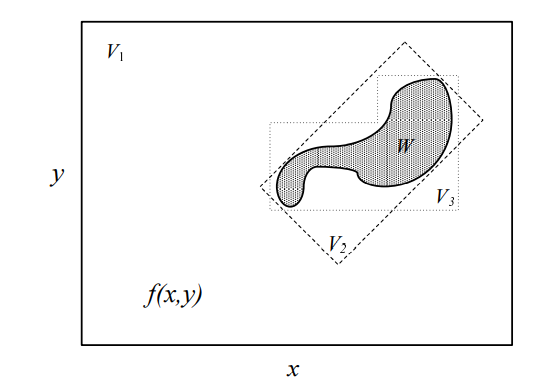
\includegraphics[width=.60\textwidth]{Montecarlo integration.PNG}}
\caption{}
\label{fig:Rejection method1}
\end{figure}

%\clearpage
\subsubsection{Importance Sampling: (da completare MATIAS)}
NB SEE PG 411 NUM REC

The volume in an hypercube is concentrated in it's outer part and is given by:
\[ V(L,n)=L^{n}\]
thus:
\[\Delta V = V(L,n) - V(L-\delta,n)\]
this implies
\[ \frac{\Delta V}{V}\sim n\frac{\delta}{L}\]
which proove the assertion that the fraction of volume increase clearly with the number of dimension and the the volume gratest part of volume will be located very close to the surface of this hypercube.

How we perform trivial estimation of integral?
We will generate point uniformly distributed in the domain of the function f upon which we are integrating.

continue\\ 
In more than three dimension integration over a Volume will become less efficient for the fact we had already mentioned. No points will be generated on the boundary of the hypercube which is the most important.

Suppose that an integrand f can be written as the product of a function h that is almost constant times another, positive, function g. Then its integral over a multidimensional volume V is:
\[\int fdV=\int\frac{f}{g}\cdot gdV = \int hgdV\]

\[I=\int f dV= \int \frac{f}{p} \cdot p dV= mean(\frac{f}{p})V \pm V\cdot Var(\frac{f}{p}) = \]
in this way we are improving the generation 

\[Var(f)= \sqrt{\frac{\langle f^2 \rangle- \langle f  \rangle^2}{N}}\]

\paragraph{The problem of correlation and Variance: How to generated an uncorrelated sample?}


Following formula is denominated partial correlation
\[\hat{R}(k)=\frac{1}{(n-k)\sigma^2}\sum^{n-k}_{t=1}\Big(X_{t}-\mu\Big)\Big(X_{t+k}-\mu\Big) \]
where for k=0 $\hat{R}(k)=1$

if i generate points using metropolis i might use a delta which gives points that are too close to each other.

\begin{figure}[h!t]
\centering
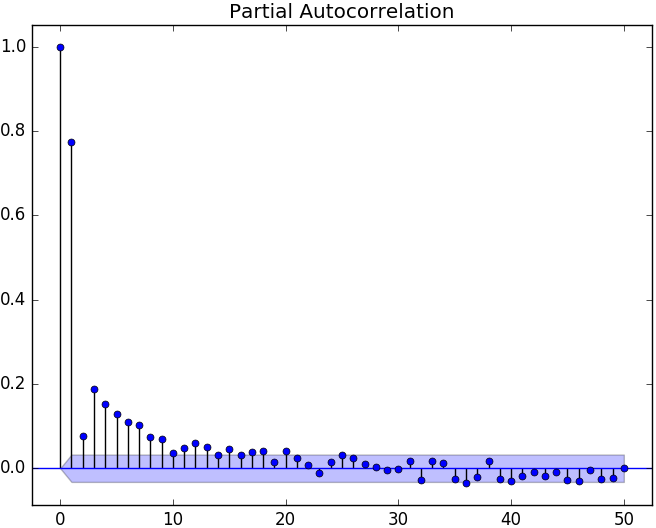
\includegraphics[scale=0.5]{Partial Autocorrelation}
\caption{}\label{PartialAutocorrelation}
\end{figure}
\chapter{Neural networks}\label{chap:3}

\section{Neural Networks (da RICONTROLLARE DIDO)}
\subsection{Introduction}
Neural networks have lot of practical application but also they have been built to mimic the behaviour of a neuron in the brain.
A neuron is connecting a certain number of entries with other neuron though the synaptic junction.
The mapping between neuron is \textbf{non-linear}, and this is because the synaptic junction is passing information to other neuron only if the signal overcome a certain threshold.

The human brain is a strongly interconnected non-linear system of neurons:
in the human cortex there are $150\cdot10^3$ neurons per $mm^2$ that correspond to about $3 \cdot 10^3$ neurons. Each neuron has about $10^4$ synaptic connections and therefore the number of synaptic connection in the human brain is about $10^{15}$.
\begin{figure}[h!t]
\centering
\subfloat[][\emph{}]
{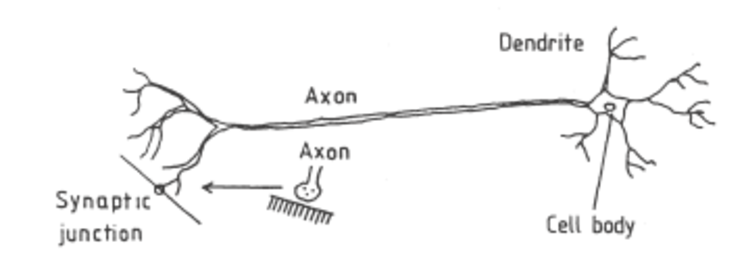
\includegraphics[width=.80\textwidth]{Immagini/Synaptic Junction.pdf}}
\caption{}
\end{figure}

Signal entering in the neuron are mixed together but the output signal is non linear, so to say, there is a filtering of the signal that is at the core of the process which through some parameters ensure that the neuron is performing well.
Both in nature and in artificial networks therefore there are parameters that need to be fixed (e.g. the threshold) to enhance the performance of the systems. But how do we manage to fix these parameters?
\paragraph{How neurons respond to stimulus: Hebb's Law}
 As originally postulated by Donald Hebb, the strength of a synaptic connection can be adjusted, if its level of activity changes. An active synapse, which repeatedly triggers the activation of its post-synaptic neuron, will grow in strength, while others will gradually weaken.
 In principle this is how in nature connection between neurons are created or destroyed. This can bee seen in figure \ref{fig:Arborization} which points out how links between neurons are strengthened or weakened in the previous years of brain life.
 \begin{figure}[h!t]
\centering
\subfloat[][\emph{}]
{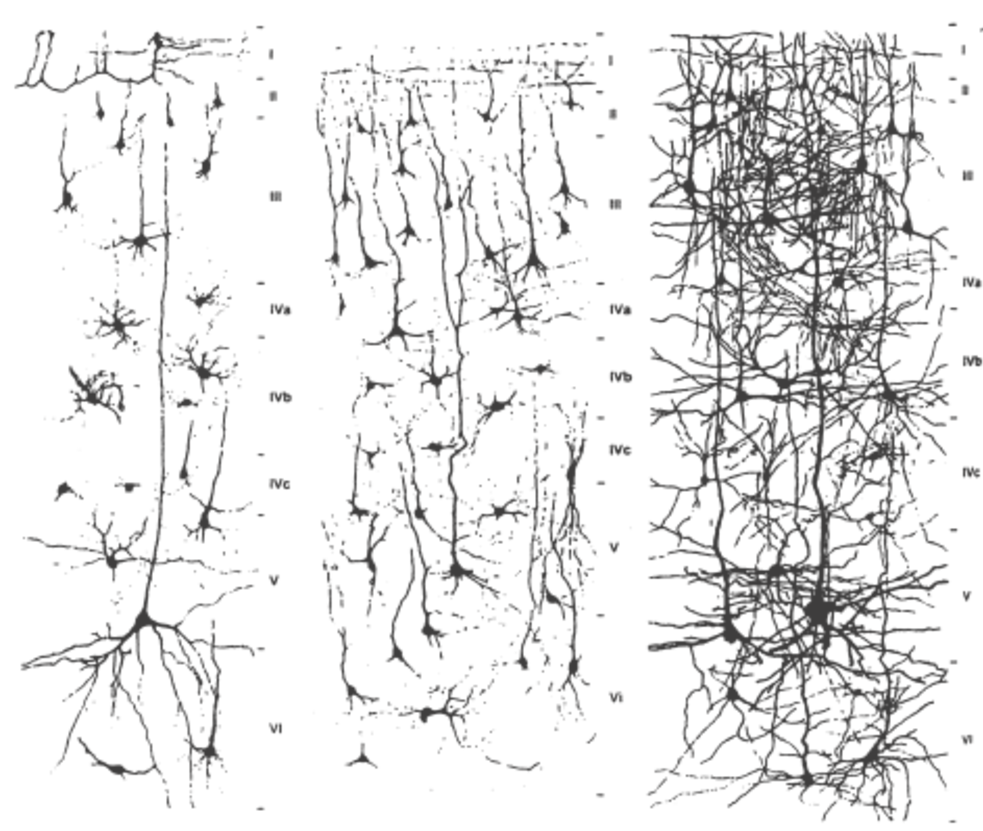
\includegraphics[width=.80\textwidth]{Immagini/DendriticHarborization.pdf}}
\caption {Development of dendritic arborization in the human visual cortex, from
(left) newborn, (middle) three-month-old, and (right) two-year-old infants }
\label{fig:Arborization}
\end{figure}


\paragraph{Brain size in animals:}
 Here it is important to relate the size of the brain to the total size of the animal. Studies in vertebrate animals have shown that the weight of the brain E grows with body weight P for species at a comparable level of evolution. Quantitatively, a quite strict relation of the form:
\begin{equation}
    Log(E)=a Log(p)+c
    \label{eq:RelationBrainSurface}
\end{equation}
with a $\sim 0.6$ was found. Since the surface of a body grows as $p=\frac{2}{3}$, one may suspect that the brain size grows in proportion to the body
surface, corresponding to the value $a = \frac{2}{3}$. This result is not too much of a
surprise, because the amount of external sensory information that the brain
has to process increases roughly in proportion to the surface of the body.
Vertebrates belonging to different levels of evolution differ, not so much in
the density of neurons, but in the magnitude of the constant of proportionality
C in the relation \ref{eq:RelationBrainSurface}.
To generalize this concept we can say that the size of the brain is scaling with the surface of the animals.

\subsection{Neural Network}\label{sec:ArtificialNeuralNetworks}
Neural network models are algorithms for cognitive tasks, such as learning and optimization, which are in a loose sense based on concepts derived from research into the nature of the brain (and thus related to the Hebb's law). In mathematical terms a neural network model is defined as a directed graph with the following properties: 
\begin{enumerate}
    \item A state variable $n_{i}$ is associated with each node $i$.
    \item A real-valued weight $w_{ik}$ is associated with each link ($ik$) between two nodes $i$ and $k$.
    \item A real-valued bias $\theta_{i}$ is associated with each node $i$.
    \item A transfer function $f(n_{k},w_{ik},\theta_i,(k\neq i)$ is defined, for each node $i$, which determines the state of the node as a function of its bias, of the weights of its incoming links, and of the states of the nodes connected to it by these links.
    
\end{enumerate}
In the standard terminology, the nodes are called neurons, the links are called synapses, and the bias is known as the activation threshold. The transfer function usually takes the form $f(\sum_{k}w_{ik}n_{k}-\theta_i)$, where $f(x)$ is either a discontinuous step function or its smoothly increasing generalization known as a sigmoidal function . Nodes without links toward them are called input neurons; output neurons are those with no link leading away from them. A feed-forward network is one whose topology admits no closed paths. It is our aim to study such models and learn what they can (and cannot) do.


In 1943 Warren McCulloch and Walter Pitts proposed general theory of information processing based on networks of binary switching or decision elements, which are somewhat euphemistically called "neurons", although they are far simpler than their real biological counterparts. Each one of these elements $i = 1, \dots , n$can only take the output values $n_{i} = 0,1$, where $n_i = 0$ represents the resting state and $n_i = 1$ the active state of the elementary unit.
In order to simulate the finite regenerative period of real neurons, changes in the state of the network are supposed to occur in discrete time steps $t = 0, 1,2, \dots$. The new state of a certain neural unit is determined by the influence of all other neurons, as expressed by a linear combination of their output values:

\begin{equation}
    h_{i}(t) = \sum_{j} w_{ij}n_{j}(t)
    \label{eq:ti}
\end{equation}
Here the matrix $w_{ij}$ represents the synaptic coupling strengths (or synaptic
efficacies) between neurons $j$ and $i$, while $h_i(t)$ models the total post-synaptic
potential at neuron $i$ caused by the action of all other neurons.
$h_i$ can be considered the input into the neural computing unit, and $n_i$ the
output. The properties of the neural network are completely determined by
the functional relation between hi(t) and $n_i(t + 1)$ . In the simplest case, the
neuron is assumed to become active if its input exceeds a certain threshold
$\theta_i$, which may well differ from one unit to the next. The \textbf{evolution of the
network} is then governed by the law

\begin{equation}
    n_{i}(t+1)=\Theta[ h_{i}(t)-\theta_{i}]
    \label{eq:ni}
\end{equation}
where $\Theta(x)$ is the unit step function.
 The network differs from a traditional computer in that the steps of the program are not executed sequentially, but in parallel within each elementary unit. One might say that the program code consists of a single statement, i.e. the combination of the
equations \ref{eq:ni} and \ref{eq:ti}. 
The extreme reduction of the program is compensated by the substitution of a vast number of processing elements ($10^{11}$ in the human brain!) for the single processing unit of a conventional, sequential electronic computer.

\subsubsection{Two simple model of neural network}

\paragraph{The perceptron}A perceptron is a specific type of neural network, but is actually a simplified model of the biological mechanisms of processing of sensory information, i.e. perception. In its simplest form, a perceptron consists of two separate layers of neurons 2 representing the input and output layer, respectively, as illustrated in Fig. \ref{fig:Simpleperceptron}. The neurons of the output layer receive synaptic signals from those of the input layer, but not vice versa, and the neurons within one layer do not communicate with each other. The flow of information is thus strictly directional; hence one speaks of a feed-forward network.
 \begin{figure}[h!t]
\centering
{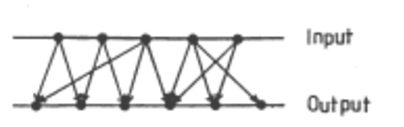
\includegraphics[width=.40\textwidth]{Immagini/SimplePerceptron.pdf}}
\caption {Simple perceptron, consisting of two layers of neurons. The input neurons feed into the neurons of the output layer, but not vice versa.}
\label{fig:Simpleperceptron}
\end{figure}

\paragraph{Ising model}
There is a similarity between a neural network of the type previously given and systems of elementary magnetic moments or spins, see
Fig. \ref{fig:Spinising}. 
In these systems, called Ising models, the spin $S_i$ at each lattice site $i$ can take only two different orientations, up or down, denoted by $S_i = +1$ (up) and $S_i = -1$ (down). The analogy to a neural network is realized by identifying each spin with a neuron and associating the upward orientation $S_i = + 1$ with the active state $n_i = 1$ and the downward orientation $S_i = -1$ with the resting state $n_i = O$.

 \begin{figure}[h!t]
\centering
{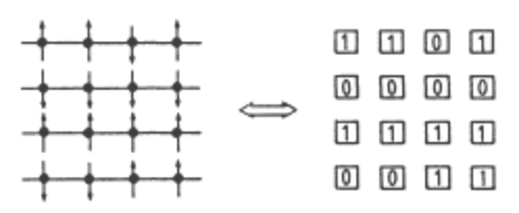
\includegraphics[width=.50\textwidth]{Immagini/SpinIsing.pdf}}
\caption {A one-to-one correspondence exists between lattices of magnetic spins with two different orientations (Ising systems) and McCulloch-Pitts neural networks. A spin pointing up (down) is identified with an active (resting) neuron.}
\label{fig:Spinising}
\end{figure}

These ideas were further developed by Little and Gordon Shaw
and by John Hopfield who studied how such a neural network or spin
system can store and retrieve information.

\paragraph{The Little and Hopfield models}
 The Little and Hopfield models differ in the manner in which the state of the system is updated. 
 \begin{itemize}
     \item  In Little's model all neurons (spins) are updated synchronously according to the law \ref{eq:ni}.
     \item  In the Hopfield model the neurons are updated sequentially one at a time (either in a certain fixed order or randomly). 
 \end{itemize}

 Sequential updating has a considerable advantage when the network is simulated on a conventional digital computer, and also for theoretical analysis of the properties of the network. On the other hand, it holds the essential conceptual disadvantage that the basic feature of neural networks, namely the simultaneous operation of a large number of parallel units, is given up. Neurons in the human brain surely do not operate sequentially, this being precisely the reason for the brain's superiority in complex tasks to even the fastest existing electronic computer.


\subsubsection{Associative memory}
Associative memory, i.e. storage and recall of information by association with
other information, may be the simplest application of "collective" computation on a neural network.

Here we define an associative memory as follows. Assume that p binary patterns containing N bits of information (i.e. p different images containing N bits for each), $\nu_{i}^{\mu}(i = 1, \dots , N;\mu=1,\dots,p)$, are stored in the to memory. If now a new pattern (not already memorized) $n_{i}$ is presented, that stored pattern $\nu_{i}^{\lambda}$ is to be recalled which most strongly resembles the presented pattern. This means that $\nu_{i}^{\lambda}$ and $n_{i}$ (which is the $i$\textsuperscript{th} bits of information of the new pattern) should differ in as few places as possible, i.e. that the mean square deviation 
 
\begin{equation}
    H_{\mu}=\sum_{i=1}^{N}(n_{i}-\nu_{i}^{\mu})^2
\end{equation}
is minimal for $\mu=\lambda$. $H_{\mu}$ is called the \textbf{Hamming distance} between the patterns $n_{i}$ and $\nu_{i}^{\mu}$.

In principle, this problem is easily solved on a standard digital computer by computing all values $H_{\mu}$ and then searching for the smallest one. However, if the memory contains many large patterns, this procedure can take quite a long time. We are therefore led to ask the question whether the patterns can be stored in a neural network of N elements (neurons) in such a way that the network evolves from the initial configuration $n_{i}$, corresponding to the presented pattern, into the desired configuration  $\nu_{i}^{\mu}$ under its own dynamics.

In order to formulate the problem, it is useful to invoke the analogy between neurons and Ising spins, mentioned before, replacing the quantities $\nu_{i}$, $n_i$ by new variables $s_{i}$, $\sigma_{i}$, which are defined as

\begin{equation}
\centering
    s_{i}=2n_{i}-1 \qquad \sigma_{i}=2\nu_{i}-1
\end{equation}
The new variables take the values $\pm1$, instead of 0 and 1 (remember that $n_{i}=0,1$). 
The squared deviations are then expressed as
\begin{equation}
    (n_{i}-\nu_{i}^{\mu})^2=\frac{1}{4}(s_{i}-\sigma_{i}^{\mu})^2=\frac{1}{4}(s_{i}^2-2 s_{i}\sigma_{i}^{\mu}+(\sigma_{i}^{\mu})^2)\underset{(\sigma_{i}^{\mu})^2=s_{i}^2=1}{=}\frac{1}{2}(1-s_{i}\sigma_{i}^{\mu})
\end{equation}
which gives a second expression for the Hamming distance in term of the new variables
\begin{equation}
     H_{\mu}=\sum_{i}\frac{1}{2}(1-s_{i}\sigma_{i}^{\mu})
\end{equation}
so $ H_{\mu}=0 \Leftrightarrow \forall i \quad s_{i}\sigma_{i}^{\mu}=1$ and thus \[s_{i}=\sigma_{i}^{\mu}\]

According to Hopfield the dynamical evolution of the state of the network is now defined as follows. The individual neurons $i$ are assigned new values $s_i(t + 1)$ in some randomly chosen sequence. The new values are computed according to the rule
\begin{equation}
    s_i(t + 1)=\sgn{\Big[\sum_{j=1}^{N}w_{ij}s_{j}(t)\Big]}
    \label{eq:evol}
\end{equation}
where the instantaneous output values of all neurons are to be taken on the right-hand side. The temporal evolution proceeds, as already mentioned in the previous chapter, in finite steps, i.e. $t$ takes only the discrete values $t = 0,1,2, \dots$. Equation \ref{eq:evol} corresponds to the rule \ref{eq:ni}, rewritten in the new variables $s_{i}$.


\subsubsection{Learning by Hebb's Rule}
The immediate problem consists in choosing the synaptic coupling strengths
$w_{ij}$ given the stored patterns $\sigma_{i}^{\mu}$, such that the network evolves from the presented pattern $s_i$ into the most similar stored pattern by virtue of its own inherent dynamics. 

For a start, we will give the solution to this problem and then prove that it really serves its purpose. In order to do so we have to show, first, that each stored pattern corresponds to a stable configuration of the network and, second, that small deviations from it will be automatically corrected by the network dynamics.
 
 Stable means not only if i provide to the network exactly the memorized pattern, the network gives it back, but also if i provide a significantly different pattern the net, it will converge to the memorized one.
 \paragraph{Single stored pattern}
We begin with the simple, but not trivial, case of a \textbf{single stored pattern} $\sigma_{i}$ (implies p=1). The state corresponding to this pattern remains invariant under the network dynamics, if $h_i =\sum_{j} w_{ij}\sigma_{j}$ has the same sign as $\sigma_{i}$.
This condition is satisfied by the simple choice
\begin{equation}
    w_{ij}=\frac{1}{N}\sigma_{i}\sigma_{j}
    \label{eq:simplelaw}
\end{equation}
in fact:
\begin{equation}
    h_i =\sum_{j}^{N} w_{ij}\sigma_{j}=\frac{1}{N}\sum_{j}^{N} \sigma_{i}(\sigma_{j})^2=\sigma_{i}\frac{1}{N}\sum_{j}^{N}1=\sigma_{i}
    \label{eq:eichi}
\end{equation}
and so 
\begin{equation}
     s_i(t + 1)=\sgn{\Big[\sigma_{i}\Big]}=\sigma_{i}=s_{i}(t)
\end{equation}
it means that the network is stable because if i give to it the memorized pattern $\sigma_{i}$ at time $t$ it gives me back exactly the same pattern $\sigma_{i}$ at time $t+1$.

We want the network to converge to the memorized pattern also if a time t we provide a pattern that is partially corrupted.
Now assume that the network would start its evolution not exactly in
the memorized state $\sigma_{i}$, but some of the elements had the wrong value (-1 instead of +1, or vice versa). Without loss of generality we can assume that these are the first n elements of the pattern,
\begin{equation}
  s_{i}(t) =
    \begin{cases}
      -\sigma_{i} & i=1,\dots,n\\
      \sigma_{i} & i=n+1,\dots,N\\
    \end{cases}       
\end{equation}
such that
\begin{equation}\begin{split}
    h_i &=\sum_{j=1}^{N} w_{ij}s_{j}(t)=\frac{1}{N}\sigma_{i}\Big[-n+(N-n)\Big]\\
    &=\big(1-\frac{2n}{N}\big)\sigma_{i}
    \label{eq:eichi2}
\end{split}
\end{equation}
 for $n < \frac{N}{2}$ the network makes the transition into the correct, stored pattern after a single update of all neurons:
\begin{equation}
     s_i(t + 1)=\text{sign}\Big[\sigma_{i}\Big]=\sigma_{i}=s_{i}(t)
\end{equation}
One also says that the stored pattern acts as an attractor (if $n < \frac{N}{2}$) or for the network dynamics, meaning that if i provide the net pattern with few wrong bit it will gives back the correct pattern.
\paragraph{Multiple stored pattern:}
We are now ready to consider the general case, where p patterns $\sigma_{1} , \dots,\sigma_{i}$ are to be stored. Generalizing eq. \ref{eq:simplelaw}, we choose the synaptic strengths according to the rule
\begin{equation}
    w_{ij}=\frac{1}{N}\sum_{\mu=1}^p\sigma_{i}^\mu \sigma_{j}^\mu
    \label{eq:simplelaw}
\end{equation}
which is usually referred to as \textbf{Hebb's rule}. 
If $\sigma_{i}^\mu=\sigma_{j}^\mu$, i.e.  if neurons $i$ and $j$ are both active or dormant for a given pattern, a positive contribution to $w_{ij}$ results. If this occurs for the majority of patterns, the synapse becomes excitatory. On the other hand, if $\sigma_{i}^\mu=-\sigma_{j}^\mu$ for most patterns, we obtain $w_{ij}<0$, i.e. the synaptic connection becomes inhibitory.
Lets now check again for the stability of the network:
\begin{equation}\begin{split}
    h_i^{(\nu)} &=\sum_{j=1}^{N}w_{ij}\sigma_{j}^\nu\\
    &=\frac{1}{N}\sum_{\mu=1}^{p}\sigma_{i}^\mu \sum_{j}^{N}\sigma_{j}^\mu \sigma_{j}^\nu\\
    &=\frac{1}{N}\Big[\sigma_{i}^\nu \sum_{j} \sigma_{i}^\nu \sigma_{i}^\nu+         \sum_{\mu \neq \nu}\sigma_{i}^\mu\sum_{j}\sigma_{j}^\mu\sigma_{j}^\nu \Big]\\
    &=\sigma_{i}^\nu+\frac{1}{N}\Big[\sum_{\mu \neq \nu}\sigma_{i}^\mu\sum_{j}\sigma_{j}^\mu\sigma_{j}^\nu \Big] \\
    &\sim \sigma_{i}^\nu+\mathcal{O}\Big(\sqrt{(p-1)/N}\Big)
\end{split}
\end{equation}

The first term is identical with the one in \ref{eq:eichi}, obtained for a single stored pattern. In the case that the stored patterns are \textbf{uncorrelated}, one sees that the second term contains in all N(p-1) randomly signed contributions (±1). Hence, according to the laws of statistics, for large N and p its value will typically be of size  $\frac{1}{N}\sqrt{N(p-1)}=\sqrt{(p-1)/N}$.\footnote{This is a consequence of the central-limit theorem: the sum of a large number, N, of independent random variables will obey a Gaussian distribution centered at N times the mean value and having a variance which is $\sqrt{N}$ times the variance of the original probability distribution.} 
As long as $p \ll N$, when the number of stored patterns is much smaller than the total number of neurons in the network, the additional term will most likely not affect the sign of the complete expression $h_{i}^{(\nu)}$, which alone determines the reaction of the $i^{th}$ neuron. \emph{The smaller the ratio $p/N$, the greater the likelihood that the pattern $\nu$ is a \textbf{stable configuration} of the network}.

Again, if n neurons start out in the "wrong" state, a combination of the previous considerations yields (recall eq. \ref{eq:eichi2})

\begin{equation}\begin{split}
    h_i^{(\nu)} &= \big(1-\frac{2n}{N}\big)\sigma_{i}^{\nu}+\frac{1}{N}\Big[\sum_{\mu \neq \nu}\sigma_{i}^\mu\sum_{j}\sigma_{j}^\mu\sigma_{j}^\nu \Big] \\
    &\sim \big(1-\frac{2n}{N}\big)\sigma_{i}^{\nu}+\mathcal{O}\Big(\sqrt{(p-1)/N}\Big)
    \end{split}
    \label{eq:morewrongpattern}
\end{equation}
Under the condition $n, p \ll N$ we will still have $\sgn(h_{i})=\sigma_{i}^{\nu}$, i.e. the network configuration will converge to the desired pattern within a single global update. However, if the number of stored patterns is comparable to the number N of neurons, the second, randomly distributed term in eq. \ref{eq:morewrongpattern} becomes of order one, and the patterns can no longer be recalled reliably. As we shall prove later with the help of powerful mathematical methods borrowed from statistical physics, this undesirable case occurs when the number p of stored random patterns exceeds $14\%$ of the number N of neurons, i.e. $p/N < 0.14$.
This limit becomes significantly higher if the various stored patterns happen to be orthogonal to each other, i.e. if their scalar products (the red part of $\frac{1}{N}\Big[\sum_{\mu \neq \nu}\sigma_{i}^\mu \textcolor{red}{\sum_{j}\sigma_{j}^\mu\sigma_{j}^\nu} \Big]$ present in eq. \ref{eq:morewrongpattern}) satisfy the conditions

\begin{equation}
    \frac{1}{N}\sum_{i}\sigma_{i}^\mu\sigma_{i}^{\mu'}=\delta_{\mu \mu'}
\end{equation}

Obviously, the disturbing "noise" term in (\ref{eq:morewrongpattern}) vanishes in this case, and hence it is possible to store and retrieve N patterns\footnote{Each pattern have N bit and so there are at most N different orthogonal patterns!}. 
As we shall see in the next paragraph, there exist "learning" protocols, i.e. rules for the choice of the synaptic connections, which are superior to Hebb's rule and permit the storage of up to 2N retrievable patterns, and which even work in the presence of correlations. However, Hebb's rule is by far the simplest and most easily implementable of learning rules.

\subsubsection{The projection rule}
As we discussed, the ability to recall memories correctly breaks down if the number p of stored patterns exceeds a certain limit. When the synaptic connections are determined according to Hebb's rule, this happens at the storage density $\alpha = p/N = 0.138$. 
The reason for this behavior was the influence of the other stored patterns as expressed by the fluctuating noise term in \ref{eq:morewrongpattern}. As we already pointed out, this influence vanishes exactly if the patterns are orthogonal to each other as defined in the previous section. On the other hand, the power of recollection deteriorates even earlier if the stored patterns are strongly correlated. Unfortunately, this happens in many practical examples. Just think of the graphical representation of roman letters, where "E" closely resembles "F" and "e" resembles "G", or of a typical list of names from the telephone book, which are probably highly correlated.

Nonetheless, it turns out that the problem of discriminating between correlated patterns has a remarkably simple solution, which even permits the storage of $p = N$ arbitrarily correlated patterns, as long as they are linearly independent. To see how it works, we form the matrix of scalar products between all pairs of patterns $(\sigma_{i}^{\mu} = \pm 1)$:

\begin{equation}
    \mathcal{Q}_{\mu\nu}=\frac{1}{N}\sum_{i}\sigma^{\mu}_{i}\sigma^{\nu}_{i}\quad (1\leq \mu, \nu\leq p)
\end{equation}

For linearly independent patterns the matrix $ \mathcal{Q}_{\mu\nu}$ is invertible, and we can define the following improved synaptic coupling strengths

\begin{equation}
    \Tilde{w}_{ij}=\frac{1}{N}\sum_{\mu,\nu}\sigma^{\mu}_{i}(\mathcal{Q}^{-1})_{\mu \nu}\sigma^{\nu}_{j}
    \label{eq:omegadef}
\end{equation}

Mathematically, \ref{eq:omegadef} corresponds to a projection technique that eliminates the existing correlations between patterns, hence this learning rule is often called the projection rule. With this choice the interaction of the stored patterns due to the fluctuating term in eq. \ref{eq:morewrongpattern} vanishes exactly, as can be easily seen by computing the post-synaptic potentials in the presence of one of the memorized patterns $\sigma^{\nu}_{j}$:

\begin{equation}
\begin{split}
    \Tilde{h}_{i}&=\sum_{j}\Tilde{w}_{ij}\sigma^{\lambda}_{j}=\frac{1}{N}\sum_{\mu,\nu}\sigma^{\mu}_{i}(\mathcal{Q}^{-1})_{\mu \nu}\sum_{j}\sigma^{\nu}_{j}\sigma^{\lambda}_{j}\\    &=\sum_{\mu,\nu}\sigma^{\mu}_{i}(\mathcal{Q}^{-1})_{\mu \nu}\mathcal{Q}^{\nu \lambda}=\sum_{\mu}\sigma^{\mu}_{i}\delta_{\mu \lambda}\\
    &=\sigma^{\lambda}_{i}
\end{split}
\end{equation}

We conclude that every stored pattern represents a stable network configuration, independent of correlations among the patterns. Of course, the condition $p \sim N$ continues to limit the memory capacity, since at most N linearly independent patterns can be formed from N units of information.
To exploit this rule one has to compute the inverse of $\mathcal{Q}_{ij}$ which is time consuming if $\mathcal{Q}_{ij}$ is not diagonal, and usually it is not as already mentioned.

\subsubsection{An iterative learning scheme}\label{Sec:DOm}
The practical application of the projection learning rule for large, memory saturated networks suffers from the need to invert the $(p \times p)$ matrix $\mathcal{Q}_{ij}$ which poses a formidable numerical problem. Fortunately, the matrix inversion need be performed only once, when the patterns are stored into the network. The ingrained memory can then be recalled as often as desired without additional effort. A practical method of implementing the projection rule is based on an iterative scheme, where the "correct" synaptic connections are strengthened in order to stabilize the correlated patterns against each other.

Because of the neuron evolution law  $s_i(t + 1)=\sgn[h_{i}(t)]$ any pattern $\sigma_{i}^{\mu}$ represents a stable network configuration, if $h_i$ has the same sign as $\sigma_{i}$, i.e. defining the \textbf{stability coefficients}

\begin{equation}
    \Tilde{\gamma}_{i \mu}=\sigma_{i}^{\mu}h_{i}=\sum_{j}w_{ij}\sigma_{i}^{\mu}\sigma_{j}^{\mu}>0
    \label{eq:htilde1}
\end{equation}

for every neuron $i$. If the expression \ref{eq:htilde1} is only slightly positive, any small perturbation, i.e. $s_{i}\neq \sigma_{i}^{\mu}$ for a few neurons $i$, can change its sign. In order to achieve greater stability of the desired memory patterns, we demand that the expression \ref{eq:htilde1} be not only positive but also greater than a certain threshold $K>O$. For a single pattern, Hebb's rule (eq \ref{eq:simplelaw}) yields $h_i = a_i$. As a consequence, the condition $a_{i}h_{i} = 1$ is always satisfied in this case. It appears natural to take the stability threshold at $K = 1$ also in the general case of several stored patterns, and to demand that the synaptic connections be chosen such that

\begin{equation}
       \Tilde{\gamma}_{i \mu}= \sigma_{i}^{\mu}h_{i}=\sum_{j}w_{ij}\sigma_{i}^{\mu}\sigma_{j}^{\mu}=1
       \label{eq:stabilitycoeff}
\end{equation}

for all neurons $i$.
An obvious method of achieving the desired result begins with choosing the synaptic connections initially according to Hebb's rule:
\begin{equation}
w_{ij}=\frac{1}{N}\sum_{\mu}\sigma^{\mu}_{i}\sigma^{\mu}_{j}    
\end{equation}

In the next step we check, one after the other for all stored patterns, whether
the condition \ref{eq:stabilitycoeff} is fulfilled. If this is not the case, we modify the synapses
according to the prescription

\begin{equation}
    w_{ij}\rightarrow w_{ij}'=w_{ij}+\delta w_{ij}
\end{equation}
with
\begin{equation}
    \delta w_{ij}=\frac{1}{N}\big(1-\sigma_{i}^{\mu} h_{i}\big)\sigma_{i}^{\mu}\sigma_{j}^{\mu}
\end{equation}
where $\mu$ denotes the pattern just under consideration.  With these modified
synaptic connections we obtain for the same pattern $\mu$
\begin{equation}
    \begin{split}
        \sigma_{i}^{\mu}h_{i}'&=\sigma_{i}^{\mu}h_{i}+\sum_{j}\delta w_{ij}\sigma_{i}^{\mu}\sigma_{j}^{\mu}\\
        &=\sigma_{i}^{\mu}h_{i}+\frac{1}{N} \sum_{j}(\sigma_{i}^{\mu})^2(\sigma_{j}^{\mu})^2(1-\sigma_{i}^{\mu}h_{i})\\
        &=\sigma_{i}^{\mu}h_{i}+1-\sigma_{i}^{\mu}h_{i}\\
        &=+1
    \end{split}
\end{equation}
since $(\sigma_{i}^{\mu})^2 = 1$. Thus, after updating all synapses, the threshold stability condition \ref{eq:stabilitycoeff} is satisfied for the considered pattern. When we proceed to the next pattern $(\mu + 1)$, the synaptic couplings will be modified again, so that  \ref{eq:stabilitycoeff} becomes valid for the pattern now under consideration. However,  \ref{eq:stabilitycoeff} may cease to be satisfied for the previous pattern $\mu$. After a full cycle over all stored patterns the condition is therefore only fulfilled with certainty for the last pattern, $\mu = p$, but not necessarily for all other patterns. The crucial question is whether this updating process converges, or whether it
may continue indefinitely without reaching a stationary state, in which the threshold condition is satisfied by all patterns.

It is possible to demonstrate that iterating the previous procedure leads to

\begin{equation}
    w_{ij}' \rightarrow \Tilde{w}_{ij}
\end{equation}
 which means that iterating $\infty$ times ensure that the network will be stable.
This procedure is called \textbf{Diederich-Opper}.


\subsubsection{Spin Glasses}\label{sec:Spinglasses}
By denoting the two possible states of a neuron by the variables $S_i = +1$ (active neuron) and $s_i = -1$ (resting neuron), we have already exposed the analogy between a neural network and a system of atomic magnetic dipoles or spins, which can be oriented in two different directions (Ising system). We shall now show how this analogy can be advantageously exploited in view of the remarkable progress made in studies of the physical properties of magnetic systems.

Atoms interact with each other by inducing a magnetic field at the location of another atom, which interacts with its spin. The total local magnetic field at the location of an atom $i$ is given by $h_i = \sum_{j}w_{ij}s_{j}$, where $w_{ij}$ is the dipole force, and the diagonal term $j = i$ (self-energy) is not included in the sum. Newtons law "action = reaction" ensures that the coupling strengths $w_{ij}$ are symmetric: $w_{ij} = w_{ji}$. In realistic cases the strength of interaction between two atoms falls off with distance r, because the dipole force falls as $1/r^3$ . In simple models of magnetic-spin systems one therefore often retains only the interaction between atoms that are nearest neighbors. If all $w_{ij}$ are positive, the material is \emph{ferromagnetic}; if there is a regular change of sign between neighboring atoms, one has an \emph{antiferromagnet}. If the signs and ab- solute values of the $w_{ij}$ are distributed randomly, the material is called a spin glass. The ferromagnetic case corresponds to a neural network that has stored a single pattern. The network which has been loaded with a large number of randomly composed patterns resembles a spin glass.

In order to describe the properties of a spin system it is useful to introduce
an energy functional $E[s]$ :

\begin{equation}
    E(s)=-\frac{1}{2}\sum_{ij}^{i \neq j}w_{ij}s_{i}s_{j}
    \label{eq:energyformula}
\end{equation}
This is always possible for symmetric couplings $w_{ij} = w_{ji}$; anyantisymmetric contribution would cancel in the double sum in \ref{eq:energyformula}.
We can include the diagonal terms $i = j$ in \ref{eq:energyformula} without prejudice since these contribute, because of $(S_i)^2 = (\pm1)^2 = 1$, only a constant term to the energy, which does
not depend on the orientation of the spins (or on the states of the neurons):
\begin{equation}
    E(s)=-\frac{1}{2}\sum_{ij}w_{ij}s_{i}s_{j}+\frac{1}{2}\sum_{i}w_{ii}
    \label{eq:additionalconstants}
\end{equation}
This additional constant does not influence the dynamical evolution of the system and can be dropped.
If the couplings $w_{ij}$ are determined according to Hebb's rule (\ref{eq:simplelaw}), and if the configuration of the system corresponds to a stored pattern $\sigma_{i}^{\mu}$, the energy functional takes the value (considering $(\sigma_{i}^{\mu})^{2}=1$)
\begin{equation}
    \begin{split}
        E(\sigma^{\nu})&=-\frac{1}{2N}\sum_{ij}\sum_{\mu}w_{ij}\sigma^{\mu}_{i}\sigma^{\mu}_{j}\sigma^{\nu}_{i}\sigma^{\nu}_{j}\\
        &=-\frac{1}{2N}\Big[N^2 +\sum_{\mu\neq \nu}\Big(\sum_{i}\sigma^{\mu}_{i}\sigma^{\nu}_{i}\Big)^2\Big]
    \end{split}
\label{eq:en1}
\end{equation}
Assuming that the patterns are uncorrelated and the values o-f = ±1 are
equally likely, one finds that the term $\sum_{i}\sigma^{\mu}_{i}\sigma^{\nu}_{i}$ $(\mu \neq \nu)$ is of order $\sqrt{N}$, and therefore the energy becomes
\begin{equation}
    \begin{split}
        E(\sigma^{\nu})&=-\frac{1}{2N}\Big[N^2 + \mathcal{O}\big((p-1)N\big)\Big]\sim -\frac{N}{2}+\mathcal{O}\Big(\frac{p-1}{2}\Big)
    \end{split}
\label{eq:en2}
\end{equation}
The influence of all other patterns $(\mu \neq \nu)$ causes a slight shift of the total energy, since it is typically caused by fluctuations around the ground state of a system. If the spins of a few atoms have the wrong orientation, the fluctuating term is replaced by another fluctuating term, which does not result in an essential modification of its magnitude. However, the term with $(\mu = \nu)$ suffers a substantial change: if the first n spins are incorrectly oriented $(s_{i} = -\sigma^{\nu}_{i}$ for $i = 1, \dots , n)$, its value changes to

\begin{equation}
    \sum_{ij}\sigma^{\mu}_{i}\sigma^{\mu}_{j}s_{i}s_{j}=\Big(N-2n\Big)^2
\end{equation}
i.e. the energy of the configuration rises in proportion to the extent of its deviation from the stored pattern:
\begin{equation}
    \begin{split}
        E(s)&\sim-\frac{1}{2N}\big(N-2n\big)^2 + \mathcal{O}\big((p-1)\big)\\
        &= E(\sigma^{\nu}) +2n-\frac{2n^2}{N}
    \end{split}
\label{eq:en2}
\end{equation}

The memorized patterns are therefore (at least local) minima of the energy functional $E[s]$.
A more detailed investigation shows that the energy functional has, in addition, infinitely many other local minima. However, all these spurious minima are less pronounced than those given by the stored patterns $\sigma^{\mu}_{i}$; hence these correspond to global minima of the energy surface $E[s]$, at least for moderate values of the parameter $\alpha = p/N$, which indicates the degree of utilization of storage capacity. 








\subsubsection{parallel versus Sequential Dynamics}
The energy function of a physical system is closely related to its dynamics. It is easy to see that the energy function $E[s]$ (eq \ref{eq:energyformula}) continually decreases with time in the case of (random) sequential updating of the neuron states (the Hopfield model). That is to say, the contribution of a given neuron $i$ to the energy (eq. \ref{eq:energyformula}) at time t is

\begin{equation}
    E_{i}(t)=-s_{i}(t)\Big[\sum_{j \neq i}w_{ij}s_{j}(t)\Big]=-s_{i}(t)h_{i}(t)
\end{equation}

If the state of the neuron $i$ is updated according to the law (3.5) its contribution to the energy becomes

\begin{equation}
\begin{split}
     E_{i}(t+1)&=-s_{i}(t+1)\Big[\sum_{j \neq i}w_{ij}s_{j}(t)\Big]=-\sgn[h_{i}(t)]h_{i}(t)=-|h_{i}(t)|\\
     &\leq -s_{i}(t)h_{i}(t) = E_{i}[t]
\end{split}
\end{equation}
In other words, the energy contribution of a given neuron never increases with time. Since the energy functional $E[s]$ is bounded below, this implies that the network dynamics must reach a stationary point that corresponds to a (local) minimum of the energy functional. The network thus always ends up in a state of equilibrium, which is stable against changes in the state of any single neuron.

%The random sequential updating of spin states was first considered as a model for the nonequlibrium statistical physics of magnetic systems by R. Glauber; one therefore also uses the term Glauber dynamics to describe the sequential mode of operation of a neural network. The approach to equilibrium becomes particularly important in the context of network models based on stochastic neurons, which are the subject of Chapt. 4. The Glauber dynamics then ensures - for an appropriate neural activation function - that the network enters a state of thermodynamic equilibrium, which can be studied with methods derived from statistical physics.
The argument given above does not apply to the synchronous mode of operation of the neural network (the Little model). Since all neurons assume new states in parallel and at the same moment, the contribution of an individual neuron to the energy function cannot be considered in isolation. In
this case it is more appropriate to consider the stability function\footnote{This is the Lyapunov function of the system.}

\begin{equation}
    E_{L}(t)=-\sum_{i,j}s_{i}(t)s_{j}(t-1)
\end{equation}
which depends on the state of the entire network at two subsequent moments of its dynamical evolution. $E_{L}[s(t);s(t-1)]$ cannot be regarded as an energy functional, since it depends on the states of the neurons at two different times, i.e. it is nonlocal in the time variable. However, for symmetric synaptic weights $w_{ij} = w{ji}$ it is again easy to show that $E_{L}(t)$ decreases monotonously
with time:
\begin{equation}\begin{split}
E_{L}(t+1)&=-\sum_{i,j}s_{i+1}(t)s_{j}(t)=-\sum_{i}\sgn[h_{i}(t)]h_{i}(t)\\
    &=\sum_{i}|h_{i}(t)|\leq \sum_{j}h_{j}(t)s(t-1)=E_{L}(t)
    \end{split}
\end{equation}

Since, on the other hand,
\begin{equation}
    E_{L}(t+1)-E_{L}(t)=-w_{ij}s_{i}(t)\Big[s_{j}(t+1)-s_{j}(t-1)\Big]
\end{equation}
the network must eventually settle into a steady state with the same network configuration being repeated every other time step: $\delta E_{L}=0 \implies s_i (t + 1) = s_i (t - 1)$. This means that the network can either reach a steady state, as in the Hopfield model, or permanently cycle between two different configurations.

\subsubsection{Neural motion pictures}\label{sec:Neuralmotionpictures}
Temporal sequences of recalled memories form a very important aspect of our mental capacity. They enable us to comprehend the course of events and actions, which otherwise would consist of meaningless single pictures. Periodic sequences of neural impulses are also of fundamental importance for the control of motor body functions, such as the heartbeat, which occurs with great regularity almost three billion times during an average person's life. Irregularities in the cardiac rhythm are fortunately rare, but cause grave concern if they do occur. The questions how neural networks can sustain highly periodic activity for a long period of time and what makes them fail under certain conditions are thus of vital interest. 
It is clear from the very beginning that here we have to study the properties of networks with aysmmetric synaptic connections, because periodic activity cannot occur in the presence of thermodynamic equilibrium, toward which all symmetric networks develop. It turns out that the transition from a Hopfield-Little network with its stable-equilibrium configurations to a network exhibiting stationary periodic activity is surprisingly simple. One only has to modify Hebb's rule (eq. \ref{eq:simplelaw}) in the following manner:


\begin{equation}
   w_{ij}=\frac{1}{N}\sum_{\mu=1}^{p}\sigma^{\mu+1}_{i}\sigma^{\mu}_{j}
   \label{eq:eqn1}
\end{equation}
where the patterns $\sigma^{+1}_{i}$ and $\sigma^{1}_{i}$ are identified in order to get temporal periodicity. In order to see how the synaptic rule (eq. \ref{eq:eqn1}) works, we assume that the network configuration is just given by one of the patterns, $s_i(t) = \sigma_{i}(t)$. Assuming that the patterns are orthogonal, the synaptic polarization potential for the next update is
\begin{equation}
    \begin{split}
        h_{i}(t)&=\sum_{j}w_{ij}\sigma^{\mu}_{j}=\frac{1}{N}\sum_{\mu}\sigma^{\mu+1}_{i}\sum_{j}\sigma^{\mu}_{j}\sigma^{\nu}_{j}=\frac{1}{N}\sum_{\mu}\sigma^{\mu+1}_{i}N\delta_{\mu \nu}\\
        \\&=\sigma^{\nu+1}_{i}
    \end{split}
\end{equation}
As a consequence the network immediately makes a transition into the next pattern, $s_i(t + 1) = \sigma^{\nu+1}_{i}$ , i.e. it performs "heteroassociation" instead of autoassociation. (Note that this mechanism works only in the synchronous, parallel updating mode.)

This rapid, undelayed transition between patterns is not always desired. In the biological context it would imply that one activation pattern would replace another on the scale of the elementary time constant of neural processes, i.e. patterns would change every few milliseconds. This is much too short for many processes, such as motor actions or chains of thoughts, where the characteristic time constants lie in the range of tenths of seconds. How is it possible to stretch the temporal separation between different patterns, to obtain a kind of "slow-motion" effect? One way to achieve this delay is to add a stabilizing term to the expression \ref{eq:eqn1} for the synaptic connections. Again Hebb's rule \ref{eq:simplelaw} does the trick, if we take the synapses as
\begin{equation}
    w_{ij}=\frac{1}{N}\sum_{\mu}\sigma^{\mu}_{i}\sigma^{\mu}_{j}+\frac{\lambda}{N}\sum_{\mu}\sigma^{\mu+1}_{i}\sigma^{\mu}_{j}
\end{equation}
If we set $A < 1$, the pattern initially remains stable, because the stabilizing Hebb term dominates; for $A > 1$ the pattern is unstable and gives way to the following patterns in the next updating step. In order to expand the time between transitions, one only has to make the parameter A time dependent
in an appropriate way. One could start out with a small value of A, let it grow until it triggers the change of patterns, then immediately reduce it to its initial small value to keep the next pattern stable, and so on.
A better, and less artificial, way to slow down the network is to introduce different types of synaptic connections with stabilizing and transition inducing tasks, characterized by different lengths of their relaxation time. We denote the rapidly relaxing, stabilizing ("fast") synapses by
\begin{equation}
     w_{ij}^{F}=\frac{1}{N}\sum_{\mu}\sigma^{\mu}_{i}\sigma^{\mu}_{j}
\end{equation}
and the slowly relaxing, change-inducing ("slow") synapses by
\begin{equation}
 w_{ij}^{S}=\frac{\lambda}{N}\sum_{\mu}\sigma^{\mu+1}_{i}\sigma^{\mu}_{j}
\end{equation}

The total post-synaptic polarization potential at time t is defined as

\begin{equation}
    h_{i}(t)=\sum_{j} \Big[ w_{ij}^{F}s_{j}(t)w_{ij}^{S}\overline{s_{j}}(t)\Big]
\end{equation}
where the "slow" synapses $w_{ij}^{S}$ average over a number of previous configura-
tions of the network:

\begin{equation}
    \overline{s_{j}}(t)=\int_{-\infty}^{t}dt'G(t-t')s(t')
\end{equation}
Here $G(t)$ plays the role of a delay function, which is normalized according
to $\int_{0}^{\infty}dt G(t) = 1$. Standard choices for this function are $G(t) = \delta(t - T)$,
representing a definite well-defined time delay (Fig. \ref{fig:exponential}a), and $G(t) =
\tau^{-1}e^{(-\frac{t}{\tau})}$, describing a gradual decay of the post-synaptic potential with
a characteristic time constant $\tau$ (Fig. \ref{fig:exponential}b ).
 \begin{figure}[h!t]
\centering
{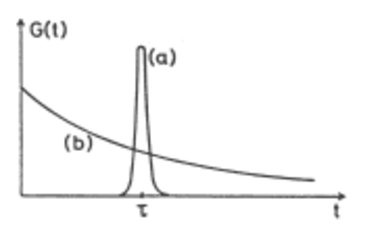
\includegraphics[width=.350\textwidth]{Immagini/exponential.pdf}}
\caption{Two possible choices (curves a and b) for the synaptic delay function G(t).}
\label{fig:exponential}
\end{figure}
For the exponential delay function the interesting range of A is between 1 and 2. The temporal distance between transitions of patterns diverges at the lower boundary $(A = 1)$, and decreases to the value $t_{0} =\tau \log(2)$ at $(A = 2)$. An interesting special case is that of a single pattern a and the synapses
\begin{equation}
    w_{ij}^{S}=-\lambda \sigma_{i}\sigma_{j} \qquad 
    w_{ij}^{S}=\sigma_{i}\sigma_{j}
\end{equation}

which cause the network to oscillate between the pattern and its inverse.
In this manner one can construct neural networks that permanently cycle between states of high and low activity. In addition to the possibility of going through periodic cycles of p patterns or of getting stuck at one of the patterns (if A is too small), a further kind of temporal behavior has been observed for the case of the exponential synaptic delay function $G(t)$ . If the parameter A is chosen sufficiently large then the network switches to chaotic time evolution, tumbling through a set of distorted patterns in a highly irregular fashion.

\subsection{Stochastic neurons}\label{sec:Stochasticneurons}
We now consider a simple generalization of the neural networks discussed in the previous sections which permits a more powerful theoretical treatment.
For this purpose we replace the deterministic evolution law
\begin{equation}\label{DeterministicNetwork}
s_i(t+1)=\sgn{\bigl[h_i(t)\bigr]}=\sgn{\left[\sum_{j=1}^Nw_{ij}s_j(t)\right]}
\end{equation}
for the neural activity by a \emph{stochastic law}, which does not assign a definite value to $s_i(t+1)$, but only gives the probabilities that $s_i(t+1)$ takes one of the values $+1$ or $-1$. In particular we request that
%\begin{equation}
%\operatorname{Pr}\bigl[s_i(t+1)\bigr]=f\bigl[h_i(t)\bigr]
%\end{equation}
\begin{equation}
\operatorname{Pr}\bigl[s_i(t+1)=+1\bigr]=f\bigl[h_i(t)\bigr]
\end{equation}
where the activation function $f(h)$ must have the proper limiting values $f(h\rightarrow-\infty)=0$, $f(h\rightarrow+\infty)=1$. Between these limits the activation function must rise monotonously. A standard choice, depicted in Figure~\ref{f(h)}, is given by
\begin{equation}\label{sigmoidal}
f(h)=\frac{1}{1+e^{-2\beta h}}
\end{equation}
which satisfies the condition
\begin{equation}
f(h)+f(-h)=1
\end{equation}
Accordingly, since $\operatorname{Pr}\bigl[s_i(t+1)=-1\bigr]=1-f\bigl[h_i(t)\bigr]$, we can explicit our stochastic law as
\begin{gather}
\operatorname{Pr}\bigl[s_i(t+1)=+1\bigr]=f\bigl[+h_i(t)\bigr]\\
\operatorname{Pr}\bigl[s_i(t+1)=-1\bigr]=f\bigl[-h_i(t)\bigr]
\end{gather}
that is the values $s_i(t+1)=\pm1$ will occur with probability $f(\pm h_i)$.

The shape of the function $f(h)$ is essentially that of a Fermi--Dirac distribution\footnote{The step is now placed at $h=0$ and unlike the Fermi function it grows monotonously.}\footnote{Such functions are often called \emph{sigmoidal} functions.}, which describes the thermal energy distribution in a system of identical fermions. In that case the parameter $\beta$ has the meaning of an inverse temperature, $\beta=T^{-1}$ (imagine the thermodynamic beta $\beta=1/(k_{\text{B}}T)$ in natural units). We shall also use this nomenclature in connection with neural networks, although this does not imply that the parameter $\beta^{-1}$ should denote a physical temperature at which the network operates. The rule \eqref{sigmoidal} should rather be considered as a model for a stochastically operating network which has been conveniently designed to permit application of the powerful formal methods of statistical physics. In other words, $\beta^{-1}$ is essentially a pseudo-temperature, i.e. an artifical parameter that has been called ``temperature'' in analogy with statistical physics, but that have a completely different meaning. Notice that in the limit $\beta\rightarrow\infty$, or $T\rightarrow0$, the Fermi function \eqref{sigmoidal} approaches the unit step function $\Theta(h)$. This means that at very low temperature the stochastic neural network goes over into our original deterministic network \eqref{DeterministicNetwork}. Hence all results obtained for stochastic networks can be extrapolated to the deterministic case.
\begin{figure}[ht]
\centering
\pgfplotsset{
layers/personal/.define layer set={axis background,axis grid,pre main,main,axis ticks,axis lines,axis tick labels,axis descriptions,axis foreground}{
	grid style				= {/pgfplots/on layer=axis grid},
	tick style				= {/pgfplots/on layer=axis ticks},
	axis line style			= {/pgfplots/on layer=axis lines},
	label style				= {/pgfplots/on layer=axis descriptions},
	legend style			= {/pgfplots/on layer=axis descriptions},
	title style				= {/pgfplots/on layer=axis descriptions},
	colorbar style			= {/pgfplots/on layer=axis descriptions},
	ticklabel style			= {/pgfplots/on layer=axis tick labels},
	axis background@ style		= {/pgfplots/on layer=axis background},
	3d box foreground style	= {/pgfplots/on layer=axis foreground},
},}
\pgfmathsetmacro{\b}{2.6}
\begin{tikzpicture}
\begin{axis}[set layers=personal,width=9cm,height=6.75cm,ylabel={$f(h)$},xlabel={$h$},axis x line=middle,axis y line=middle,x label style={at={(ticklabel* cs:1)},anchor=west},y label style={at={(ticklabel* cs:1)},anchor=south},xmin=-2,xmax=2,ymin=-1.5,ymax=1.8,xtick={-1/\b,1/\b},xticklabels={$-\dfrac{1}{\beta}$,$+\dfrac{1}{\beta}$},ytick={-1,1},yticklabels={$-1$,$+1$}]
\draw[lightgray,dashed] (axis cs:0,1) -- (axis cs:2,1);
\draw[lightgray,dashed] (axis cs:-1/\b,0) -- (axis cs:-1/\b,{1/(1+e^(-2*\b*(-1/\b)))});
\draw[lightgray,dashed] (axis cs:+1/\b,0) -- (axis cs:+1/\b,{1/(1+e^(-2*\b*(+1/\b)))});
\addplot[very thick,smooth,samples=80,domain=-2:2]{1/(1+e^(-2*\b*x))};
\end{axis}
\end{tikzpicture}
\caption{}\label{f(h)}
\end{figure}

The exact state of a given neuron in a stochastic network is not of particular relevance, because it is determined randomly. However, the \emph{mean activity} of a neuron (or the mean orientation of a spin in the magnetic analogy) is an interesting quantity. Let us first consider a single neuron; its mean activity is given by
\begin{equation}
\begin{split}
\langle s\rangle&=(+1)f(h)+(-1)f(-h)\\
&=\frac{1}{1+e^{-2\beta h}}-\frac{1}{1+e^{2\beta h}}\\
&=\frac{1}{1+e^{-2\beta h}}-\frac{e^{-2\beta h}}{1+e^{-2\beta h}}\\
&=\frac{1-e^{-2\beta h}}{1+e^{-2\beta h}}\\
&=\frac{e^{\beta h}-e^{-\beta h}}{e^{\beta h}+e^{-\beta h}}\\
&=\tanh{(\beta h)}
\end{split}
\end{equation}
As already said, in the limit $\beta\rightarrow\infty$ one obtains $\langle s\rangle=\sgn{(h)}$, i.e., depending on the sign of the local field $h$, the neuron is either permanently active or permanently dormant (again, we recover the deterministic result).
\begin{figure}[ht]
\centering
\pgfplotsset{
layers/personal/.define layer set={axis background,axis grid,pre main,main,axis ticks,axis lines,axis tick labels,axis descriptions,axis foreground}{
	grid style				= {/pgfplots/on layer=axis grid},
	tick style				= {/pgfplots/on layer=axis ticks},
	axis line style			= {/pgfplots/on layer=axis lines},
	label style				= {/pgfplots/on layer=axis descriptions},
	legend style			= {/pgfplots/on layer=axis descriptions},
	title style				= {/pgfplots/on layer=axis descriptions},
	colorbar style			= {/pgfplots/on layer=axis descriptions},
	ticklabel style			= {/pgfplots/on layer=axis tick labels},
	axis background@ style		= {/pgfplots/on layer=axis background},
	3d box foreground style	= {/pgfplots/on layer=axis foreground},
},}
\pgfmathsetmacro{\b}{3}
\begin{tikzpicture}
\begin{axis}[set layers=personal,width=9cm,height=6.75cm,ylabel={$\langle s\rangle$},xlabel={$h$},axis x line=middle,axis y line=middle,x label style={at={(ticklabel* cs:1)},anchor=west},y label style={at={(ticklabel* cs:1)},anchor=south},xmin=-2,xmax=2,ymin=-1.65,ymax=1.65,xtick={-1/\b,1/\b},xticklabels={$-\dfrac{1}{\beta}$\hspace*{15pt},$+\dfrac{1}{\beta}$},ytick={1,-1},yticklabels={$+1$,$-1$},y tick label style={outer sep={0.02pt+0.13em},inner sep={0.33333em-0.13em},fill=white,fill opacity=0.75,text opacity=1,xshift={mod(\ticknum,2)*2.385em},/pgfplots/on layer=axis ticks}]
\draw[lightgray,dashed] (axis cs:-2,1) -- (axis cs:2,1);
\draw[lightgray,dashed] (axis cs:-2,-1) -- (axis cs:2,-1);
%\draw[lightgray,dashed] (axis cs:-1/\b,0) -- (axis cs:-1/\b,{1/(1+e^(-2*\b*(-1/\b)))});
%\draw[lightgray,dashed] (axis cs:+1/\b,0) -- (axis cs:+1/\b,{1/(1+e^(-2*\b*(+1/\b)))});
\addplot[very thick,smooth,samples=80,domain=-2:2]{tanh(\b*x)};
\end{axis}
\end{tikzpicture}
\caption{The function $\langle s\rangle=\tanh{(\beta h)}$.}\label{mean(s)}
\end{figure}

The evolution of a single neuron $i$ in a network composed of many elements is difficult to describe, since its state depends on \emph{all} other neurons, which continually fluctuate between $+1$ and $-1$. That even remains true if we are only interested in the mean activity of the $i$-th neuron. This is determined by the value of the synaptic potential $h_i$, which depends, however, on the actual instantaneous states $s_j$ of the other neurons and not on their mean activities. The difficulty is a result of the non-linearity of the probability function $f(h)$, which does not permit one to take the average in the argument of the function. In such cases one often resorts to a technique called the \textbf{mean-field approximation}.

We have already seen the mean-field approximation in many contexts: in solid state physics, statistical physics and nuclear physics also. In those cases we used to study many-body problems (for example systems of interacting fermions) of which we were given the total Lagrangian. By solving the Euler--Lagrange equations, one is able to construct a system of (often coupled) equations which then had to be solved to determine the evolution of the individual fields. The problem arises from the fact that usually we work in a quantum regime, and not in a classical one; so the fields to be determined are actually operators, and not numbers. An operator is a more complicated object because it contains a lot of information, although one usually takes the expectation value to get some measure of probability. Consequently, the interaction terms within the equations of motion become almost unmanageable for many-body problems, as each field depends on the local value of all the other fields. The idea of the mean-field approximation is therefore to systematically reduce quantum fields into classical fields, that is to see them no longer as operators, but as numbers. In practice, instead of quantum fields, their expectation value was substituted: $\widehat{\psi}\rightarrow\langle\widehat{\psi}\rangle$. In this way the many-body problem is simplified in a one-body problem, because the total intricate interaction is replaced with a \emph{mean field} generated by all the others (i.e. no more many-body-dependent). In other words, this technique allows us to factor out the terms of interactions and to obtain, by adding them, a single interaction field that describes the average potential generated by all the particles together. The mean-field approximation becomes particularly useful when we have to deal simultaneously with many bodies (indeed, it is sometimes called large-$N$ approximation).

Returning to our neural networks, here we basically want to do the same thing, and therefore we can define the mean-field approximation as the exchange operation between the synaptic potential with its average value
\begin{equation}
f(h_i)\xrightarrow{\text{MFA}}f\bigl(\langle h_i\rangle\bigr)=f\!\left(\sum_{j=1}^Nw_{ij}\langle s_j\rangle\right)
\end{equation}
The mean activity of a neuron is then computable as before:
\begin{equation}
\langle s_i\rangle=(+1)f\bigl(\langle h_i\rangle\bigr)+(-1)f\bigl(-\langle h_i\rangle\bigr)
\end{equation}
whence
\begin{equation}\label{StochasticNetwork}
\boxed{\langle s_i\rangle=\tanh{\left(\beta\sum_{j=1}^Nw_{ij}\langle s_j\rangle\right)}}
\end{equation}
This is still a system of nonlinear equations with $N$ unknowns $\langle s_i\rangle$, but these have become deterministic rather than stochastic variables.
\subsubsection{Single pattern}
The solution of the system of equations \eqref{StochasticNetwork} depends, of course, on the choice of the synaptic strengths $w_{ij}$. We begin by considering the simplest case of a single pattern
\begin{equation}
w_{ij}=\frac{1}{N}\sigma_i\sigma_j
\end{equation}
Assuming also that all bits are equal ($+1$ or $-1$, it doesn't matter) we can further simplify it as $w_{ij}=1/N$ for all $i, j$. One could be skeptical about this assumption, but it is essentially a gauge transformation, since it corresponds to a reinterpretation of the meaning of ``up'' and ``down'' at each lattice site.

Anyway, in this case equation \eqref{StochasticNetwork} becomes
\begin{equation}
\langle s_i\rangle=\tanh{\left(\beta\frac{1}{N}\sum_{j=1}^N\langle s_j\rangle\right)}\qquad\text{for all $i$}
\end{equation}
and because the right-hand side does not depend on $i$ we can write
\begin{equation}\label{TranscendentalEquation}
\langle s\rangle=\tanh{\bigl(\beta\langle s\rangle\bigr)}
\end{equation}
(of course $\langle s_i\rangle=\langle s_j\rangle$ since we don't have any reason to suppose they are different). We have thus managed to reduce the evolution law to a single equation, but is still a transcendental equation; therefore we must solve it graphically, i.e. we have to find graphically the possible intersections between the straight line $\langle s\rangle$ and the hyperbolic tangent $\tanh{\bigl(\beta\langle s\rangle\bigr)}$. Recall that the hyperbolic tangent is monotonously increasing and from 0 to $\infty$ its slope always diminishes (vice versa, from $-\infty$ to $0$ it systemically increases, due to symmetry reason). Based on this observation, we deduce that we have to compare the behavior of the two functions at the origin, where the slope has its maximum value. In particular, we have to distinguish two cases illustrated in Figure~\ref{Intersections}. For $\beta<1$ ($T>1$) equation \eqref{TranscendentalEquation} admits only the trivial solution at $\langle s\rangle=0$ because the slope of the line is higher than that of the hyperbolic tangent (Fig.~\ref{1Solution}). So at large temperature the bits continuously flip between $+1$ and $-1$, but with null expectation value, meaning that the network is essentially unable to memorize any information. Instead, for $\beta>1$ ($T<1$) equation \eqref{TranscendentalEquation} admits altogether three solutions, namely $\langle s\rangle=-\overline{s},0,\overline{s}$ because the slope of the line is smaller than that of the hyperbolic tangent (Fig.~\ref{3Solutions}). However, it is possible to show that $\langle s\rangle=\pm\overline{s}$ correspond to a stable minimum configurations of the system, while $\langle s\rangle=0$ corresponds to a local maximum, which is unstable! In fact, the hyperbolic tangent is very stiff close to 0; hence any small perturbation from $\langle s\rangle=0$ makes the system change rapidly either towards $-1$ or $+1$. Therefore, we neglect this possibility at low temperature. Finally, the limiting situation is that in which the straight line is exactly tangent to the hyperbolic tangent, corresponding to $\beta=T=1$ (which takes the role of critical, or Curie, temperature separating the two different regimes). This analytical behavior at $T=1$ is indeed very similar to a \emph{phase transition} in which at high temperature the system is chaotic, whereas at low temperature it presents an oriented structure (like ferromagnetism).
\begin{figure}[ht]
\centering
\pgfplotsset{
	layers/personal/.define layer set={axis background,axis grid,axis ticks,axis lines,axis tick labels,axis descriptions,pre main,main,axis foreground}{
		grid style				= {/pgfplots/on layer=axis grid},
		tick style				= {/pgfplots/on layer=axis ticks},
		axis line style			= {/pgfplots/on layer=axis lines},
		label style				= {/pgfplots/on layer=axis descriptions},
		legend style			= {/pgfplots/on layer=axis descriptions},
		title style				= {/pgfplots/on layer=axis descriptions},
		colorbar style			= {/pgfplots/on layer=axis descriptions},
		ticklabel style			= {/pgfplots/on layer=axis tick labels},
		axis background@ style		= {/pgfplots/on layer=axis background},
		3d box foreground style	= {/pgfplots/on layer=axis foreground},
	},}
\begin{subfigure}[ht]{0.49\textwidth}
	\centering
        \pgfmathsetmacro{\b}{0.95}
	\begin{tikzpicture}
	\begin{axis}[set layers=personal,width=8cm,height=6.75cm,ylabel={$g\bigl(\langle s\rangle\bigr)$},xlabel={$\langle s\rangle$},axis x line=middle,axis y line=middle,x label style={at={(ticklabel* cs:1)},anchor=west},y label style={at={(ticklabel* cs:1)},anchor=south},xmin=-2,xmax=2,ymin=-1.65,ymax=1.65,xtick=\empty,ytick={1,-1},yticklabels={$+1$,$-1$},y tick label style={outer sep={0.02pt+0.13em},inner sep={0.33333em-0.13em},fill=white,fill opacity=0.75,text opacity=1,xshift={mod(\ticknum,2)*2.385em},/pgfplots/on layer=main}]
	\addplot[lightgray,dashed,samples=2,domain=-2:2,on layer=axis grid] {1};
	\addplot[lightgray,dashed,samples=2,domain=-2:2,on layer=axis grid] {-1};
	\addplot[very thick,smooth,samples=80,domain=-2:2]{tanh(\b*x)};
	\addplot[very thick,blue,samples=2,domain=-2:2]{x};
	\addplot[only marks,mark=*,mark size=3pt,mark options={fill=white}] coordinates {(0,0)};
	\end{axis}
	\end{tikzpicture}
        \caption{$\beta<1$: only one solution.}\label{1Solution}
\end{subfigure}
\hfill
\begin{subfigure}[ht]{0.49\textwidth}
	\centering
	\pgfmathsetmacro{\b}{3}
	\begin{tikzpicture}
	\begin{axis}[set layers=personal,width=8cm,height=6.75cm,ylabel={$g\bigl(\langle s\rangle\bigr)$},xlabel={$\langle s\rangle$},axis x line=middle,axis y line=middle,x label style={at={(ticklabel* cs:1)},anchor=west},y label style={at={(ticklabel* cs:1)},anchor=south},xmin=-2,xmax=2,ymin=-1.65,ymax=1.65,xtick={0.9994902,-0.9994902},xticklabels={$\overline{s}$,$\overline{s}$},ytick={1,-1},yticklabels={$+1$,$-1$},x tick label style={outer sep={0.02pt+0.13em},inner sep={0.33333em-0.13em},fill=white,fill opacity=0.75,text opacity=1,yshift={mod(\ticknum,2)*1.585em},/pgfplots/on layer=main},y tick label style={outer sep={0.02pt+0.13em},inner sep={0.33333em-0.13em},fill=white,fill opacity=0.75,text opacity=1,xshift={mod(\ticknum,2)*2.385em},/pgfplots/on layer=main}]
	\addplot[lightgray,dashed,samples=2,domain=-2:2,on layer=axis grid] {1};
	\addplot[lightgray,dashed,samples=2,domain=-2:2,on layer=axis grid] {-1};
	\addplot[lightgray,dashed,on layer=axis grid] coordinates {(-0.9994902,0) (-0.9994902,-0.9994902)};
	\addplot[lightgray,dashed,on layer=axis grid] coordinates {(0.9994902,0) (0.9994902,0.9994902)};
	\addplot[very thick,smooth,samples=80,domain=-2:2]{tanh(\b*x)};
	\addplot[very thick,blue,samples=2,domain=-2:2]{x};
	\addplot[only marks,mark=*,mark size=3pt,mark options={fill=white}] coordinates {(-0.9994902,-0.9994902) (0,0) (0.9994902,0.9994902)};
	\end{axis}
	\end{tikzpicture}
        \caption{$\beta>1$: three solutions.}\label{3Solutions}
\end{subfigure}
\caption{Intersections between $\langle s\rangle$ and $\tanh{\bigl(\beta\langle s\rangle\bigr)}$.}\label{Intersections}
\end{figure}
\subsubsection{Several patterns}
We now turn to the general situation, when the synaptic couplings are fixed according to Hebb's rule
\begin{equation}
w_{ij}=\frac{1}{N}\sum_{\mu=1}^p\sigma_i^\mu\sigma_j^\mu
\end{equation}
for several patterns. The mean-field equation \eqref{StochasticNetwork} then takes the form
\begin{equation}\label{Several patternsEq}
\langle s_i\rangle=\tanh{\left(\frac{\beta}{N}\sum_{j=1}^N\sum_{\mu=1}^p\sigma_i^\mu\sigma_j^\mu\langle s_j\rangle\right)}
\end{equation}
This relation does not have an obvious solution. However, we recall that every single stored pattern represents a stable configuration for a deterministic network. It is, therefore, not unreasonable to make the \emph{ansatz}\footnote{An ansatz (from German) is an educated guess or an additional assumption made to help solve a problem, and which is later verified to be part of the solution by its results.} that $\langle s_i\rangle$ resembles one of the stored patterns, except for a normalization factor:
\begin{equation}
\langle s_i\rangle=m\sigma_i^\nu
\end{equation}
Inserting this into \eqref{Several patternsEq} and assuming as usual that the memorized patterns are completely uncorrelated we obtain
\begin{equation}
\begin{split}
m\sigma_i^\nu&=\tanh{\left(\frac{\beta m}{N}\sum_{j=1}^N\sum_{\mu=1}^p\sigma_i^\mu\sigma_j^\mu\sigma_j^\nu\right)}\\
&=\tanh{\left(\frac{\beta m}{N}\sum_{j=1}^N\sigma_i^\nu\overbrace{\sigma_j^\nu\sigma_j^\nu}^{=1}+\frac{\beta m}{N}\sum_{\mu\neq\nu}\sigma_i^\mu\sum_{j=1}^N\sigma_j^\mu\sigma_j^\nu\right)}\\
&=\tanh{\left[\beta m\sigma_i^\nu+\beta m\mathcal{O}\Biggl(\sqrt{\frac{p-1}{N}}\Biggr)\right]}
\end{split}
\end{equation}
As long as $p\ll N$ the second term is clearly negligible:
\begin{equation}
m\sigma_i^\nu\simeq\tanh{(\beta m\sigma_i^\nu)}
\end{equation}
Moreover, on account of $\sigma_i^\nu=\pm1$, i.e. $\tanh{(-x)}=-\tanh{x}$ (it is an odd function), the normalization factor $m$ (and consequently $\langle s_i\rangle$) is determined by the same equation
\begin{equation}
m=\tanh{(\beta m)}
\end{equation}
Again we find the same fixed points as for a single stored pattern: for $T>1$ one has $m=0$, and the time-averaged network configuration does not resemble one of the stored patterns. One might say that the network is ``amnesic''. For $T<1$ one has $m=\pm\overline{s}$ and the average configuration of the network points toward one of the stored patterns. Since these take only the values $\pm1$, the patterns can be uniquely (up to an overall sign) recovered from the averaged state $\langle s_i\rangle$ of the network.

Numerical simulations as well as statistical analysis show that the number of stored patterns relative to the number of neurons, $\alpha=p/N$, plays a similar role as the parameter $T$. When the storage utilization $\alpha$ is increased starting from zero, i.e. if more and more patterns are stored, the recall quality of the network deteriorates slightly. However, when $\alpha$ approaches the critical capacity $\alpha_c\approx0.138$, the network suddenly and catastrophically fails to recall any of the memorized patterns. In other words the networks suddenly jumps from almost perfect memory into a state of complete confusion.

In order to obtain a complete description of the ability of a stochastic Hopfield network to recall memorized patterns one has to consider $m$ as function of $\alpha$ as well as of $T$. One then obtains a complete phase diagram of
the \emph{order parameter} $m(T,\alpha)$. The phase boundary between ``functioning memory'' and total ``confusion'' or ``amnesia'' is given by a line in the $\alpha$--$T$ diagram, depicted in Figure~\ref{OrderParameter}. For $T=0$ this line begins at $\alpha_c\approx0.138$ and ends, as we just have found, at $T=1$ for $\alpha=0$. At the phase boundary $m$ falls discontinuously to zero, except for $T= 0$, where the change is continuous, but not differentiable\footnote{Note that these results strictly apply only in the thermodynamic limit $N\rightarrow\infty$, i.e. for systems with infinitely many neurons.}.
\begin{figure}[h!t]
\centering
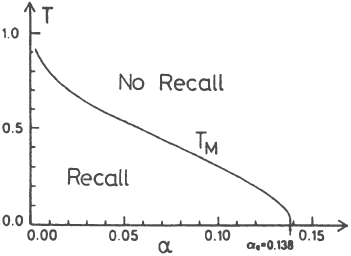
\includegraphics[scale=0.85]{Order Parameter}
\caption{Memory recall is possible only in a finite region of temperatures $T$ and storage density $\alpha=p/N$.}\label{OrderParameter}
\end{figure}

In addition to its usefulness in the formal treatment of neural-network properties the introduction of a stochastic neuron evolution law has important practical advantages. The thermal fluctuations reduce the probability that the network becomes caught in a spurious, undesired locally stable configuration.
\subsection{Special Learning Rules}\label{sec:Speciallearningrules}
As we discussed in previous sections, the standard learning rule (Hebb's rule) leads to the emergence of undesirable local minima in the ``energy'' functional $E[s]$. In practice, this means that the evolution of the network can be caught in spurious, locally stable configurations. Large networks usually contain a vast number of such spuriously stable states, many of which are not even linear combinations of the desired stability points. Even the learning rule for correlated patterns discussed in Section~\ref{Sec:DOm} does not guard against this problem. Thermal fluctuations do help to destabilize the spurious configurations, but at the expense of storage capacity. Moreover, the disappearance of all the spurious states at some finite $T$ is not ensured.

A much better strategy is to eliminate the undesired stable configurations by appropriate modifications of the synaptic connections. Hopfield et al. have proposed to make use of the fact that the spurious minima of the energy functional $E[s]$ are usually much shallower than the minima that correspond to the learned patterns. Borrowing ideas developed in the study of human dream sleep\footnote{The sleep is commonly divided in two phases, referred to as REM (rapid eye movement) and non-REMs, which is a collection of other stages. The REM phase is characterized by random rapid movement of the eyes, accompanied by low muscle tone throughout the body, and the propensity of the sleeper to dream vividly. Modern studies believe that the purpose of dream sleep (REM sleep) is the elimination of undesirable states of memory.}, they suggested tracking these states by starting the network in some randomly chosen initial configuration and running it until it ends up in a stable equilibrium state $s_i^\infty$. This may be one of the regular learned patterns, or one of the many spurious states. Then, we build new synaptic connections according to the new Hebb's rule:
\begin{equation}\label{REM}
w_{ij}\rightarrow w_{ij}-\frac{\lambda}{N}s_i^\infty s_j^\infty
\end{equation}
where $\lambda\ll1$ is chosen (indeed we are weakening connections), and we let the network run again, until it reaches another equilibrium state $s_i^\infty$. After we build another $w_{ij}$ and we let evolve, and so on and so forth. This iterative procedure must be repeated a large number of times, until we actually fall in one of the global minima. Note that whatever the resulting state is in each iteration, through \eqref{REM} the synapses are partially weakened at each step. This procedure of unlearning has two favorable effects. Most spurious equilibrium states of the network are ``forgotten'', since they are already destabilized by small changes in the synaptic connections $w_{ij}$. Moreover, the different regions of stability of the stored patterns become more homogeneous in size, since those with a larger range of stability occur more often as final configurations and are therefore weakened more than others.

The effect of this intentional forgetting is especially apparent in the sizes of the ``basins of attraction''. This term denotes the set of all states, from which the network dynamics leads to a particular pattern (e.g. $\sigma^\mu$). The change of the size of the basin of attraction of a given stored pattern, as the total memory load $\alpha=p/N$ is increased, is illustrated in Figure~\ref{BasinofAttraction}. The two axes labeled $H_k$ and $H_{N-k}$ in these figures represent a crude measure of the distance of an initial trial state $s_i$ from the considered memory state $\sigma_i^\mu$. They denote the partial Hamming distances between the trial state and the memory state, evaluated for the first $k$ and the last $N-k$ of all $N=200$ neurons (for instance), respectively:
\begin{gather}
H_{k}=\frac{1}{4}\sum_{i=1}^{k}{\bigl(s_i-\sigma_i^\mu\bigr)}^2\\
H_{N-k}=\frac{1}{4}\sum_{i=k}^{N-k}{\bigl(s_i-\sigma_i^\mu\bigr)}^2
\end{gather}
In this specific case $k=N/2$ was taken, i.e. the axes represent the Hamming distance for the first and the last half of the neurons of the network. If the trial state $s_i$ developed into the stored pattern $\sigma_i^\mu$, a black dot was plotted.

For a single memory state (Fig.~\hyperref[BasinofAttraction]{\ref*{BasinofAttraction}a}), half of the trial states are found to evolve into the stored pattern $\sigma_i$, while the other half ends up in the complementary pattern $-\sigma_i$. The basin of attraction thus represents a black triangle. This is essentially the result that we have discussed in Section~\ref{LHR}: if we have only one pattern, a random configuration of the network with some altered bits converges to the stored pattern if the number of wrong bits $n$ is smaller than $N/2$. And indeed, any set of $s_i$ (i.e. any different trial configuration) which produces a couple $(H_k,H_{N-k})$ inside the black triangle satisfies this constraint, thus converging to the stored pattern $\sigma_i$. On the other hand, if those trial states are outside the triangle, meaning they are nearer to the complementary pattern $-\sigma_i$ than $\sigma_i$, then the net will converge to $-\sigma_i$ (which is not what we want). Just to make things clearer, if we take a trial state giving $(H_k,H_{N-k})=(100,0)$, then the network configuration will develop into the memorized pattern because it means that half of the initial bits are exact ($H_{N-k}=0$), while the other half are wrong ($H_{k}=100$).

What now happens if we increase the number of stored patterns? For more memory states the basin of attraction shrinks rapidly and takes on a highly ragged shape in the vicinity of $\alpha_c\approx0.138$, as shown in Figures~\hyperref[BasinofAttraction]{\ref*{BasinofAttraction}b,\,c} for 28 and 32 uncorrelated memory states, respectively. In fact, when we are above the critical storage threshold $\alpha_c$ the network becomes no more able to retrieve memorized patterns.

Finally Figure~\hyperref[BasinofAttraction]{\ref*{BasinofAttraction}d} shows the result of applying the forgetting algorithm \eqref{REM} 1000 times to the network loaded with 32 patterns and $\lambda=0.01$. The basin of attraction grows strongly (by a factor of ten or more) and also takes on a more regular shape. The probability of retrieving the stored patterns is much improved (so ``forgetting improves the memory'').
\begin{figure}[h!t]
\centering
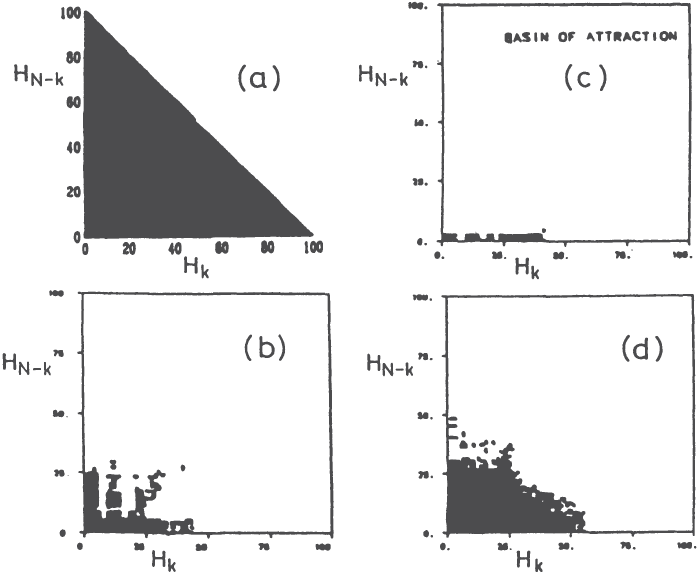
\includegraphics[scale=0.75]{Basin of Attraction}\hspace{7pt}
\caption{Basins of attraction in a Hopfield network with 200 neurons for (a) 1, (b) 28, (c) 32 memory states. After deliberate forgetting the basin expands strongly (d).}\label{BasinofAttraction}
\end{figure}

{\small
In a somewhat modified version of this method the network is allowed to develop from the stored patterns, deteriorated by random noise. One then not only weakens the synaptic connections by unlearning the final state $s_i^\infty$, but also simultaneously relearns the correct starting pattern $\nu$:
\begin{equation}\label{REMmodified}
w_{ij}\rightarrow w_{ij}-\frac{\lambda}{N}\Bigl(s_i^\infty s_j^\infty-\sigma_i^\nu\sigma_j^\nu\Bigr)
\end{equation}
If the pattern was recalled without fault, the synapses remain unchanged according to this prescription. With this method the storage capacity can be increased to $\alpha=1$, and the storage of strongly correlated patterns becomes possible.\par}

\section{Perceptrons}
\subsection{Simple perceptron}\label{Sec:SimplePerceptron}
The neural network models discussed so far were all aimed at storing and recalling given information. Memory is an important function of the brain, but far from the only one. Another important task of the central nervous system is to learn reactions and useful behavior that permit survival in an often hostile environment. In a highly simplified perspective one may identify this role of the brain with that of the supervising element in a control circuit. We shall therefore introduce the term \emph{cybernetic networks} for neural networks that provide an optimal reaction or answer to an external stimulus. Such networks usually have a structure that fundamentally differs from that of memory networks. In particular, the synaptic connections are generally not symmetric ($w_{ij}\neq w_{ji}$); often they are maximally asymmetric, i.e. unidirectional. As a result, the theories of thermodynamic equilibrium systems have no direct application to cybernetic networks, and much less general insights are known into their behavior.
%\begin{equation}
%w_{ij}=\frac{1}{N}\sum_{\mu=1}^p\sigma_i^\mu\sigma_j^\mu=w_{ji}
%\end{equation}

The best-studied class of cybernetic networks are the so-called \emph{feed-forward layered} neural networks, or simply \textbf{perceptrons}, where information flows in one direction between several distinct layers of neurons, as illustrated in Figure~\ref{Perceptron}. At one end is the \emph{input} layer composed of sensory neurons, which receive external stimuli, at the other end is an \emph{output} layer often composed of motor neurons, which cause the desired reaction.
\begin{figure}[h!t]
\centering
\pgfmathsetmacro{\h}{1.5}
\pgfmathsetmacro{\x}{1.0}
\begin{tikzpicture}[line width=0.2pt]
\draw[lightgray!30,line width=1mm,line cap=round] (-0.6,0) -- (6.6,0);
%\draw[lightgray!30,line width=1mm,line cap=round] (-0.6,-1.2) -- (6.6,-1.2);
%\draw[lightgray!30,line width=1mm,line cap=round] (-0.6,-2.4) -- (6.6,-2.4);
\draw[lightgray!30,line width=1mm,line cap=round] (-0.6,-3*\h) -- (6.6,-3*\h);
\fill[top color=lightgray!30,bottom color=lightgray!30,middle color=lightgray!5,line join=round] (-0.65,-2*\h-0.05) rectangle (6.65,-1*\h+0.05);
%\foreach \i in {0,...,3,4.5} {
%	\fill[ball color=white] (\i+0.5,-4/3*\h) circle (0.2);
%	\fill[white,opacity=0.9] (\i+0.5,-4/3*\h) circle (0.2);
%}
%\foreach \i in {0,...,3,4.5} {
%	\fill[ball color=white] (\i+0.5,-5/3*\h) circle (0.2);
%	\fill[white,opacity=0.9] (\i+0.5,-5/3*\h) circle (0.2);
%}
\foreach \i in {0,...,3,4.5} {
	\fill[ball color=white] (\i+0.5,-1.5*\h) circle (0.2);
	\fill[white,opacity=0.9] (\i+0.5,-1.5*\h) circle (0.2);
}
%Stimuli, Reaction
\foreach \i in {0,...,4,5.5} {\draw[-stealth,very thick] (\i*\x,1.1) -- (\i*\x,0.3);}
\draw[decorate,decoration={brace,amplitude=5pt},thick] (-0.2,1.2) -- (5.7,1.2) node[midway,anchor=south,inner sep=0pt,yshift=0.3cm]{External stimuli};
\foreach \i in {1,...,3,4.5} {\draw[-stealth,very thick] (\i*\x,-3*\h) -- (\i*\x,-3*\h-1.05);}
\draw[decorate,decoration={brace,mirror,amplitude=5pt},thick] (0.8,-3*\h-1.15) -- (4.7,-3*\h-1.15) node[midway,anchor=north,inner sep=0pt,yshift=-0.3cm]{Reaction};
%Input->Hidden
\draw[-stealth] (0,0) --+ ({-atan(\h/0.5)}:{sqrt((\h)^2+(0.5*\x)^2)-0.25});
\draw[-stealth] (0,0) --+ ({-atan(\h/1.5)}:{sqrt((\h)^2+(1.5*\x)^2)-0.25});
\draw[-stealth] (0,0) --+ ({-atan(\h/2.5)}:{sqrt((\h)^2+(2.5*\x)^2)-0.25});
\draw[-stealth] (0,0) --+ ({-atan(\h/3.5)}:{sqrt((\h)^2+(3.5*\x)^2)-0.25});
\draw[-stealth] (0,0) --+ ({-atan(\h/5.0)}:{sqrt((\h)^2+(5.0*\x)^2)-0.25});
\draw[-stealth] (\x,0) --+ ({180+atan(\h/0.5)}:{sqrt((\h)^2+(0.5*\x)^2)-0.25});
\draw[-stealth] (\x,0) --+ ({-atan(\h/0.5)}:{sqrt((\h)^2+(0.5*\x)^2)-0.25});
\draw[-stealth] (\x,0) --+ ({-atan(\h/1.5)}:{sqrt((\h)^2+(1.5*\x)^2)-0.25});
\draw[-stealth] (\x,0) --+ ({-atan(\h/2.5)}:{sqrt((\h)^2+(2.5*\x)^2)-0.25});
\draw[-stealth] (\x,0) --+ ({-atan(\h/4.0)}:{sqrt((\h)^2+(4.0*\x)^2)-0.25});
\draw[-stealth] (2*\x,0) --+ ({180+atan(\h/1.5)}:{sqrt((\h)^2+(1.5*\x)^2)-0.25});
\draw[-stealth] (2*\x,0) --+ ({180+atan(\h/0.5)}:{sqrt((\h)^2+(0.5*\x)^2)-0.25});
\draw[-stealth] (2*\x,0) --+ ({-atan(\h/0.5)}:{sqrt((\h)^2+(0.5*\x)^2)-0.25});
\draw[-stealth] (2*\x,0) --+ ({-atan(\h/1.5)}:{sqrt((\h)^2+(1.5*\x)^2)-0.25});
\draw[-stealth] (2*\x,0) --+ ({-atan(\h/3.0)}:{sqrt((\h)^2+(3.0*\x)^2)-0.25});
\draw[-stealth] (3*\x,0) --+ ({180+atan(\h/2.5)}:{sqrt((\h)^2+(2.5*\x)^2)-0.25});
\draw[-stealth] (3*\x,0) --+ ({180+atan(\h/1.5)}:{sqrt((\h)^2+(1.5*\x)^2)-0.25});
\draw[-stealth] (3*\x,0) --+ ({180+atan(\h/0.5)}:{sqrt((\h)^2+(0.5*\x)^2)-0.25});
\draw[-stealth] (3*\x,0) --+ ({-atan(\h/0.5)}:{sqrt((\h)^2+(0.5*\x)^2)-0.25});
\draw[-stealth] (3*\x,0) --+ ({-atan(\h/2.0)}:{sqrt((\h)^2+(2.0*\x)^2)-0.25});
\draw[-stealth] (4*\x,0) --+ ({180+atan(\h/3.5)}:{sqrt((\h)^2+(3.5*\x)^2)-0.25});
\draw[-stealth] (4*\x,0) --+ ({180+atan(\h/2.5)}:{sqrt((\h)^2+(2.5*\x)^2)-0.25});
\draw[-stealth] (4*\x,0) --+ ({180+atan(\h/1.5)}:{sqrt((\h)^2+(1.5*\x)^2)-0.25});
\draw[-stealth] (4*\x,0) --+ ({180+atan(\h/0.5)}:{sqrt((\h)^2+(0.5*\x)^2)-0.25});
\draw[-stealth] (4*\x,0) --+ ({-atan(\h/1.0)}:{sqrt((\h)^2+(1.0*\x)^2)-0.25});
\draw[-stealth] (5.5*\x,0) --+ ({180+atan(\h/5.0)}:{sqrt((\h)^2+(5.0*\x)^2)-0.25});
\draw[-stealth] (5.5*\x,0) --+ ({180+atan(\h/4.0)}:{sqrt((\h)^2+(4.0*\x)^2)-0.25});
\draw[-stealth] (5.5*\x,0) --+ ({180+atan(\h/3.0)}:{sqrt((\h)^2+(3.0*\x)^2)-0.25});
\draw[-stealth] (5.5*\x,0) --+ ({180+atan(\h/2.0)}:{sqrt((\h)^2+(2.0*\x)^2)-0.25});
\draw[-stealth] (5.5*\x,0) --+ ({180+atan(\h/0.5)}:{sqrt((\h)^2+(0.5*\x)^2)-0.25});
%Hidden->Hidden
\draw[-stealth,dashed,gray!60] (0.5*\x,-1*\h) --+ (-90:{\h-0.25});
\draw[-stealth,dashed,gray!60] (0.5*\x,-1*\h) --+ ({-atan(\h/1.0)}:{sqrt((\h)^2+(1.0*\x)^2)-0.25});
\draw[-stealth,dashed,gray!60] (0.5*\x,-1*\h) --+ ({-atan(\h/2.0)}:{sqrt((\h)^2+(2.0*\x)^2)-0.25});
\draw[-stealth,dashed,gray!60] (0.5*\x,-1*\h) --+ ({-atan(\h/3.0)}:{sqrt((\h)^2+(3.0*\x)^2)-0.25});
\draw[-stealth,dashed,gray!60] (0.5*\x,-1*\h) --+ ({-atan(\h/4.5)}:{sqrt((\h)^2+(4.5*\x)^2)-0.25});
\draw[-stealth,dashed,gray!60] (1.5*\x,-1*\h) --+ ({180+atan(\h/1.0)}:{sqrt((\h)^2+(1.0*\x)^2)-0.25});
\draw[-stealth,dashed,gray!60] (1.5*\x,-1*\h) --+ (-90:{\h-0.25});
\draw[-stealth,dashed,gray!60] (1.5*\x,-1*\h) --+ ({-atan(\h/1.0)}:{sqrt((\h)^2+(1.0*\x)^2)-0.25});
\draw[-stealth,dashed,gray!60] (1.5*\x,-1*\h) --+ ({-atan(\h/2.0)}:{sqrt((\h)^2+(2.0*\x)^2)-0.25});
\draw[-stealth,dashed,gray!60] (1.5*\x,-1*\h) --+ ({-atan(\h/3.5)}:{sqrt((\h)^2+(3.5*\x)^2)-0.25});
\draw[-stealth,dashed,gray!60] (2.5*\x,-1*\h) --+ ({180+atan(\h/2.0)}:{sqrt((\h)^2+(2.0*\x)^2)-0.25});
\draw[-stealth,dashed,gray!60] (2.5*\x,-1*\h) --+ ({180+atan(\h/1.0)}:{sqrt((\h)^2+(1.0*\x)^2)-0.25});
\draw[-stealth,dashed,gray!60] (2.5*\x,-1*\h) --+ (-90:{\h-0.25});
\draw[-stealth,dashed,gray!60] (2.5*\x,-1*\h) --+ ({-atan(\h/1.0)}:{sqrt((\h)^2+(1.0*\x)^2)-0.25});
\draw[-stealth,dashed,gray!60] (2.5*\x,-1*\h) --+ ({-atan(\h/2.5)}:{sqrt((\h)^2+(2.5*\x)^2)-0.25});
\draw[-stealth,dashed,gray!60] (3.5*\x,-1*\h) --+ ({180+atan(\h/3.0)}:{sqrt((\h)^2+(3.0*\x)^2)-0.25});
\draw[-stealth,dashed,gray!60] (3.5*\x,-1*\h) --+ ({180+atan(\h/2.0)}:{sqrt((\h)^2+(2.0*\x)^2)-0.25});
\draw[-stealth,dashed,gray!60] (3.5*\x,-1*\h) --+ ({180+atan(\h/1.0)}:{sqrt((\h)^2+(1.0*\x)^2)-0.25});
\draw[-stealth,dashed,gray!60] (3.5*\x,-1*\h) --+ (-90:{\h-0.25});
\draw[-stealth,dashed,gray!60] (3.5*\x,-1*\h) --+ ({-atan(\h/1.5)}:{sqrt((\h)^2+(1.5*\x)^2)-0.25});
\draw[-stealth,dashed,gray!60] (5.0*\x,-1*\h) --+ ({180+atan(\h/4.5)}:{sqrt((\h)^2+(4.5*\x)^2)-0.25});
\draw[-stealth,dashed,gray!60] (5.0*\x,-1*\h) --+ ({180+atan(\h/3.5)}:{sqrt((\h)^2+(3.5*\x)^2)-0.25});
\draw[-stealth,dashed,gray!60] (5.0*\x,-1*\h) --+ ({180+atan(\h/2.5)}:{sqrt((\h)^2+(2.5*\x)^2)-0.25});
\draw[-stealth,dashed,gray!60] (5.0*\x,-1*\h) --+ ({180+atan(\h/1.5)}:{sqrt((\h)^2+(1.5*\x)^2)-0.25});
\draw[-stealth,dashed,gray!60] (5.0*\x,-1*\h) --+ (-90:{\h-0.25});
%Hidden->Output
\draw[-stealth] (0.5*\x,-2*\h) --+ ({-atan(\h/0.5)}:{sqrt((\h)^2+(0.5*\x)^2)-0.25});
\draw[-stealth] (0.5*\x,-2*\h) --+ ({-atan(\h/1.5)}:{sqrt((\h)^2+(1.5*\x)^2)-0.25});
\draw[-stealth] (0.5*\x,-2*\h) --+ ({-atan(\h/2.5)}:{sqrt((\h)^2+(2.5*\x)^2)-0.25});
\draw[-stealth] (0.5*\x,-2*\h) --+ ({-atan(\h/4.0)}:{sqrt((\h)^2+(4.0*\x)^2)-0.25});
\draw[-stealth] (1.5*\x,-2*\h) --+ ({180+atan(\h/0.5)}:{sqrt((\h)^2+(0.5*\x)^2)-0.25});
\draw[-stealth] (1.5*\x,-2*\h) --+ ({-atan(\h/0.5)}:{sqrt((\h)^2+(0.5*\x)^2)-0.25});
\draw[-stealth] (1.5*\x,-2*\h) --+ ({-atan(\h/1.5)}:{sqrt((\h)^2+(1.5*\x)^2)-0.25});
\draw[-stealth] (1.5*\x,-2*\h) --+ ({-atan(\h/3.0)}:{sqrt((\h)^2+(3.0*\x)^2)-0.25});
\draw[-stealth] (2.5*\x,-2*\h) --+ ({180+atan(\h/1.5)}:{sqrt((\h)^2+(1.5*\x)^2)-0.25});
\draw[-stealth] (2.5*\x,-2*\h) --+ ({180+atan(\h/0.5)}:{sqrt((\h)^2+(0.5*\x)^2)-0.25});
\draw[-stealth] (2.5*\x,-2*\h) --+ ({-atan(\h/0.5)}:{sqrt((\h)^2+(0.5*\x)^2)-0.25});
\draw[-stealth] (2.5*\x,-2*\h) --+ ({-atan(\h/2.0)}:{sqrt((\h)^2+(2.0*\x)^2)-0.25});
\draw[-stealth] (3.5*\x,-2*\h) --+ ({180+atan(\h/2.5)}:{sqrt((\h)^2+(2.5*\x)^2)-0.25});
\draw[-stealth] (3.5*\x,-2*\h) --+ ({180+atan(\h/1.5)}:{sqrt((\h)^2+(1.5*\x)^2)-0.25});
\draw[-stealth] (3.5*\x,-2*\h) --+ ({180+atan(\h/0.5)}:{sqrt((\h)^2+(0.5*\x)^2)-0.25});
\draw[-stealth] (3.5*\x,-2*\h) --+ ({-atan(\h/1.0)}:{sqrt((\h)^2+(1.0*\x)^2)-0.25});
\draw[-stealth] (5.0*\x,-2*\h) --+ ({180+atan(\h/4.0)}:{sqrt((\h)^2+(4.0*\x)^2)-0.25});
\draw[-stealth] (5.0*\x,-2*\h) --+ ({180+atan(\h/3.0)}:{sqrt((\h)^2+(3.0*\x)^2)-0.25});
\draw[-stealth] (5.0*\x,-2*\h) --+ ({180+atan(\h/2.0)}:{sqrt((\h)^2+(2.0*\x)^2)-0.25});
\draw[-stealth] (5.0*\x,-2*\h) --+ ({180+atan(\h/0.5)}:{sqrt((\h)^2+(0.5*\x)^2)-0.25});
%Neurons
\foreach \i in {0,...,4,5.5} {\fill[ball color=white] (\i,0) circle (0.2);}
\foreach \i in {0,...,3,4.5} {\fill[ball color=white] (\i+0.5,-1*\h) circle (0.2);}
\foreach \i in {0,...,3,4.5} {\fill[ball color=white] (\i+0.5,-2*\h) circle (0.2);}
\foreach \i in {0,...,2,3.5} {\fill[ball color=white] (\i+1,-3*\h) circle (0.2);}
%Ellipsis dots
\foreach \i in {-1,0,1} {\fill[black] (4.75*\x+\i*0.15,0) circle (0.025);}
\foreach \i in {-1,0,1} {\fill[black] (4.25*\x+\i*0.15,-1*\h) circle (0.025);}
\foreach \i in {-1,0,1} {\fill[black] (4.25*\x+\i*0.15,-2*\h) circle (0.025);}
\foreach \i in {-1,0,1} {\fill[black] (3.75*\x+\i*0.15,-3*\h) circle (0.025);}
%Nodes
\node[anchor=west,inner sep=0pt,align=left] at (7.1,0) {Input\\[0pt]layer};
\draw[decorate,decoration={brace,mirror,amplitude=5pt},thick] (6.85,-2*\h-0.2) -- (6.85,-1*\h+0.2) node[midway,anchor=west,inner sep=0pt,align=left,xshift=0.4cm]{Hidden\\[0pt]layers};
\node[anchor=west,inner sep=0pt,align=left] at (7.1,-3*\h) {Output\\[0pt]layer};
\end{tikzpicture}
\caption{Schematic view of a feed-forward layered neural network (perceptron). The arrows represent the synaptic couplings $w$.}\label{Perceptron}
\end{figure}

In principle a perceptron can contain an arbitrary number of layers of neurons in addition to the input and output layers, but only rather simple cases have been studied in depth. Here we begin with the so-called \emph{simple perceptron}, where the input layer feeds directly into the output layer without the intervention of inner, or ``\emph{hidden}'', layers of neurons. We shall denote the states of the input neurons by $\sigma_k$, ($k=1,\ldots,N_{\text{in}}$); those of the output neurons are labeled by $S_i$, ($i=1,\ldots,N_{\text{out}}$). The activation of the output neurons by the input layer may be determined by the nonlinear function $f$ as
\begin{equation}\label{SiPerceptron}
S_i=f(h_i)=f\!\left(\sum_{k=1}^{N_{\text{in}}}w_{ik}\sigma_k\right)
\end{equation}
where $h_i$ is the linear combination
\begin{equation}\label{hPerceptron}
h_i=\sum_{k=1}^{N_{\text{in}}}w_{ik}\sigma_k
\end{equation}
The fact that the variables $\sigma_k$ occur only on the right-hand side of this relation, while the $S_i$ occur only on the left-hand side, is expression of the directedness of the networks: information is fed from the input layer into the neurons of the output layer, but not vice versa. The function $f(h)$ may be considered either a stochastic law, where it determines the probability of the values $S_i=\pm1$, or as a continuous function, if the neurons are assigned analog values (deterministic network). Here we concentrate on the latter case.
%Here we concentrate on the latter case, for which a standard choice of function is
%\begin{equation}
%f(h)=\tanh{(\beta h)}
%\end{equation}

%Pippone sulle interpolazioni e fitting totalmente inutile
%{{rec[45]%Interpolation or Fitting function: small number of parameters, but approximately similar to the desire. If to much parameters we are overfitting, which is essentially a interpolation
%How to optimize w (non linear fitting)?}}

The task now is to choose the synaptic connections $w_{ik}$ in such a way that a certain input $\sigma_k$ leads to the desired reaction, specified by the correct states of the neurons in the output layer, which we denote by $S_i=\zeta_i$. Of course, this condition must not only be satisfied for a single input, but for a number of cases (i.e. different external stimuli) indicated by the superscript $\mu$: $S_i^\mu\equiv S_i\bigl[\sigma_k^\mu\bigr]=\zeta_i^\mu$ with $\mu=1,\ldots,p$. In other words, we want to optimize the network through a suitable choice of the coupling $w_{ik}$ such that it is able to get the desired output reaction. An explicit function allowing the calculation of the $w_{ik}$ from the input $\sigma_k^\mu$ and the desired output $\zeta_i^\mu$ is not known. However, it is possible to construct \emph{iterative} procedures which converge to the desired values of synaptic connections, if those exist in principle. For this purpose it is more appropriate to start from the expression
\begin{equation}
D=\frac{1}{2}\sum_{\mu=1}^p\sum_{i=1}^{N_{\text{out}}}{\bigl(S_i^\mu-\zeta_i^\mu\bigr)}^2
\end{equation}
which is a sort of Hamming distance between the actual and the correct output. Since we want the output layers $S_i^\mu$ to produce the correct reaction $\zeta_i^\mu$, for all $\mu$, our goal clearly becomes the \emph{minimization} of $D$.

The idea is to start with an initial random choice of $w_{ik}$. Then, at each step we compute the distance $D$ and we update $w_{ik}$ by adding a correction $\delta w_{ik}$ which leads to a \emph{lowering} of $D$. Graphically, we could imagine the following situation (Fig.~\ref{GradientImage}). Suppose we have a function $f(x)$ describing the distance we are trying to minimize in order to obtain the desired reaction. Let's call $x_0$ the state of the synaptic connections corresponding to a minimum configuration of $f$ (i.e. leading to $S_i^\mu=\zeta_i^\mu$) and suppose we are actually in the state $x$ ($S_i^\mu\neq\zeta_i^\mu$). The derivative of $f(x)$ in $x$ has a certain sign: if $f'(x)>0$ (positive slope), this means that we have to move leftwards, i.e. towards smaller values of $x$, in order to reduce the function $f$; similarly, if $f'(x)<0$ (negative slope), then we have to move rightwards towards larger values of $x$ in order to lower $f$. Mathematically speaking, we can write this observation as
\begin{equation}\label{Gradient1}
x_{n+1}=x_n-\varepsilon f'(x_n)
\end{equation}
where $x_{n+1}$ is the final point we reach by moving of a quantity $\varepsilon f'(x)$, which constitutes one single step of our iterative procedure. The factor $\varepsilon$ is an arbitrary positive constant that should be chosen sufficiently small to avoid overshooting the goal. Clearly, from \eqref{Gradient1} we see that the signs are correct: if $f'(x)>0$ we move leftwards, and indeed $x_{n+1}<x_{n}$ (and vice versa). So at each step we evaluate the derivative and depending on its sign we move in the optimal direction to reduce $f$. In the limit of a large number of iterations we should expect to converge to $x_0$, the desired minimum. This reasoning is one dimension, but in our case $f$ must be identified with $D$, which is a multivariate function since it depends on the various couplings $w_{ik}$. Accordingly, we have to replace \eqref{Gradient1} with the more general form
\begin{equation}\label{Gradient2}
\mathbf{x}_{n+1}=\mathbf{x}_n-\varepsilon{\boldsymbol{\nabla}f(\mathbf{x})\bigr|}_{\mathbf{x}=\mathbf{x}_n}
\end{equation}
The method works because the gradient always points in the direction of strongest change of the function; hence the negative gradient follows the direction of steepest descent. For this reason, this method is sometimes referred to as ``gradient learning''.
\begin{figure}[h!t]
\centering
\begin{tikzpicture}
\begin{axis}[set layers=personal,width=8cm,height=6.75cm,ylabel={$f(x)$},xlabel={$x$},axis x line=middle,axis y line=middle,x label style={at={(ticklabel* cs:1)},anchor=west},y label style={at={(ticklabel* cs:1)},anchor=south},xmin=-1,xmax=5.6,ymin=-0.5,ymax=6,xtick={2,3.5,4.2},xticklabels={$x_0$,$x_{n+1}$,$x_n$},ytick=\empty]
\addplot[dashed,lightgray,on layer=axis grid] coordinates {(2,0) (2,1.3)};
\addplot[dashed,lightgray,on layer=axis grid] coordinates {(3.5,0) (3.5,2.65)};
\addplot[dashed,lightgray,on layer=axis grid] coordinates {(4.2,0) (4.2,4.204)};
\addplot[very thick,smooth,samples=20,domain=-1:5] {0.6*(x-2)^2+1.3};
\addplot[only marks,mark=*,mark size=3pt,mark options={fill=white}] coordinates {(2,1.3) (3.5,2.65) (4.2,4.204)};
\end{axis}
\draw[semithick,-latex] (4.65,3.75) --+ (241.8:1);
\end{tikzpicture}
\caption{}\label{GradientImage}
\end{figure}

At this point all that remains is to effectively apply these observations to our case of simple perceptron. First of all, with the help of \eqref{SiPerceptron} we obtain the deviation $D$ as an explicit function of the synaptic connections:
\begin{equation}
D[w_{ik}]=\frac{1}{2}\sum_{\mu=1}^p\sum_{i=1}^{N_{\text{out}}}{\Bigl[\zeta_i^\mu-f\bigl(h_i^\mu\bigr)\Bigr]}^2=\frac{1}{2}\sum_{\mu=1}^p\sum_{i=1}^{N_{\text{out}}}{\left[\zeta_i^\mu-f\!\left(\sum_{k=1}^{N_{\text{in}}}w_{ik}\sigma_k^\mu\right)\right]}^2
\end{equation}
where $h_i\equiv h_i^\mu$ is a function of $\mu$. In order to lower the value of $D$, we now compute the gradient with respect to the synaptic couplings:
\begin{equation}
\frac{\partial D}{\partial w_{ik}}=-\sum_{\mu=1}^p\Bigl[\zeta_i^\mu-f\bigl(h_i^\mu\bigr)\Bigr]f'\bigl(h_i^\mu\bigr)\frac{\partial h_i^\mu}{\partial w_{ik}}=-\sum_{\mu=1}^p\Delta_i^\mu\sigma_k^\mu
\end{equation}
with the abbreviation
\begin{equation}
\Delta_i^\mu\coloneqq\Bigl[\zeta_i^\mu-f\bigl(h_i^\mu\bigr)\Bigr]f'\bigl(h_i^\mu\bigr)
\label{eq:deltaimu}
\end{equation}
Here $f'\bigl(h_i^\mu\bigr)$ denotes the derivative of the function $f$ evaluated at the point $h_i^\mu$. Moreover we have exploited the usual chain rule to differentiate\footnote{If $f(x_1,\ldots,x_n)$, then $\displaystyle\frac{\mathrm{d}f}{\mathrm{d}x_k}=\sum_{i=1}^n\frac{\partial f}{\partial x_i}\frac{\partial x_i}{\partial x_k}$}. Finally, if we apply the gradient expression \eqref{Gradient2} we obtain the small deviation
\begin{equation}
\delta w_{ik}=-\varepsilon\frac{\partial D}{\partial w_{ik}}=\varepsilon\sum_{\mu=1}^p\Delta_i^\mu\sigma_k^\mu
\end{equation}
In conclusion, our iterative technique to obtain the desired reactions $S_i^\mu=\zeta_i^\mu$ can be summarized as follows: 
\begin{empheq}[left={\empheqlbrace},box=\boxed]{align}
&w_{ik}\rightarrow w_{ik}+\delta w_{ik}\\
&\delta w_{ik}=-\varepsilon\frac{\partial D}{\partial w_{ik}}=\varepsilon\sum_{\mu=1}^p\Delta_i^\mu\sigma_k^\mu
\end{empheq}
where the first equation indicates the small modifications we make to the synaptic couplings at each step, while the second one explicitly gives us a recipe for how to calculate them. We call this procedure the \textbf{training phase} (or routine) of the network.

At the beginning of this section we have said that the function $f(h)$ may be considered either as a stochastic law or a deterministic law, for which a standard choice of function is
\begin{equation}
f(h)=\tanh{(\beta h)}
\end{equation}
An important thing is that $f(h)$ does not necessarily need to be continuous if the right precautions are taken. For example, if we chose $f(h)=\sgn{(h)}$ we would have a potential problem in computing the derivative (as prescribed by the perceptron learning rule), since the sign function presents a jump at $h=0$. Hence we would have $f'(h)=2\delta(h)$, which is not a good situation because we don't want to deal with Dirac delta functions. However, this is an apparent problem: in practice where the derivative is not well-defined (in the sense of ``standard'' derivative) we can substitute $f'(h)$ with any arbitrary number because so much the arbitrariness of this choice is automatically absorbed in the arbitrariness of the constant $\varepsilon$. So we can choose the combination $\varepsilon f'(h)$ in order to obtain the best result. This is to say that having a continuous function is not strictly binding.

This \emph{perceptron learning rule} is rather general and works also for more complex neural networks with hidden layers of neurons. But not all that glitters is gold. This technique has also some weaknesses. First of all, the usual problem of local minima where the system can get stuck is still present because the algorithm is essentially an hill-climbing algorithm in which the steps always point to the nearest minimum. Therefore, if we have more than one local minimum, this procedure could bring us towards one of these false minima, which are not our desired output.

Second, the procedure may have a very slow convergence, if not completely absent. In fact, if we are in a point $x$ very close to the minimum $x_0$ and the step (which is a combination of the free parameter $\varepsilon$ and the derivative) goes beyond the minimum, we end up in a configuration where the sign of the derivative is changed. Then, if we iterate and the step is still larger than the necessary, we again exceeds the minimum in going in the opposite direction (with respect to the previous step). It is obvious that, if this situation does not halt, the system is found in a configuration in which it alternatively makes one step to the right and to left of the minimum. The result is a continuous jumping between the two sides which can greatly slow down the convergence towards the desired state, or even make it impossible. A possible way out is to combine the step $\Delta_n\coloneqq-\varepsilon f'(x_n)$ we would take at the present time with the step $\Delta_{n+1}\coloneqq-\varepsilon f'(x_{n-1})$ taken at the previous iteration (which is usually discarded):
\begin{equation}
\overline{\Delta}_n=\alpha\Delta_n+(1-\alpha)\Delta_{n-1}
\end{equation}
leading to $x_{n+1}=x_n+\overline{\Delta}_n$. Since the two combined steps have different signs close to the minimum their contributions are mutually canceled, thus avoiding the undesired bouncing. Of course, if we are far from the minimum, subsequent steps all point towards it and this corrective step is not so important.
\subsection{The exclusive-\texorpdfstring{\textsc{or}}{ᴏʀ} (\texorpdfstring{\textsc{xor}}{xᴏʀ}) gate}\label{sec:Theexclusivexor}
The existence of a simple but effective learning algorithm for perceptrons without hidden neurons makes these very attractive as neural-network models. Unfortunately, there exist elementary problems that cannot be handled by such a system. Let's consider for simplicity a deterministic perceptron with just two input neurons and one output neuron (Fig.~\ref{PerceptronXOR}). Is this network architecture able to reproduce any type of function, in particular logical functions (for example) like \textsc{and}, \textsc{or}, \textsc{xor} gates?
\begin{figure}[h!t]
\centering
\begin{tikzpicture}[neuron/.style={draw,thick,shape=rectangle,line join=round,minimum size=0.8cm,inner sep=0pt,outer sep=0pt}]
\node[neuron] (i1) at (0,0) {$\sigma_1$};
\node[neuron] (i2) at (2.4,0) {$\sigma_2$};
\node[neuron] (o) at (1.2,-2.4) {$S$};
\begin{scope}[on background layer]
\draw[semithick,-Stealth] (i1) --node[pos=0.5,left,xshift=-0.775mm] {$w_1$} (o);
\draw[semithick,-Stealth] (i2) --node[pos=0.5,right,xshift=0.775mm] {$w_2$} (o);
\end{scope}
\node[inner sep=0pt,anchor=west] at (3.7,0) {Input neurons};
\node[inner sep=0pt,anchor=west] at (3.7,-2.4) {Output neuron};
%\draw[-stealth] (-0.85,1.5) --+ ({-atan(1.5/0.85)}:{sqrt((1.5)^2+(0.85)^2)-0.25});
%\draw[-stealth] (0.85,1.5) --+ ({180+atan(1.5/0.85)}:{sqrt((1.5)^2+(0.85)^2)-0.25});
%\fill[ball color=white] (-0.85,1.5) circle (0.2);
%\fill[ball color=white] (0.85,1.5) circle (0.2);
%\fill[ball color=white] (0,0) circle (0.2);
%\node[inner sep=0pt,anchor=south] at (-0.85,1.85) {$\sigma_1$};
%\node[inner sep=0pt,anchor=south] at (0.85,1.85) {$\sigma_2$};
%\node[inner sep=0pt,anchor=north] at (0,-0.35) {$S$};
%\node at (-0.75,0.6) {$w_1$};
%\node at (0.8,0.6) {$w_2$};
%\node[inner sep=0pt,anchor=west] at (2,1.5-0.035) {Input neurons};
%\node[inner sep=0pt,anchor=west] at (2,0-0.035) {Output neuron};
\end{tikzpicture}
\caption{}\label{PerceptronXOR}
\end{figure}

Before answering, let's recall how they are defined. The result of the logical \textsc{and} (symbol $\land$) between a certain number of variables is 1 if all the variables are 1, while it is 0 if even just one variable is 0. Instead, the result of the logical \textsc{or} (symbol $\lor$) between a certain number of variables is 1 if at least one variable is 1, while it is 0 if all the variables are equal to 0. If more than one variable is 1, the result is always 1. The possible results of these two functions between our two input neurons are shown in Tables~\ref{AND} and \ref{OR}, respectively (they are called truth tables). Notice that the definitions are given in terms of the Boolean variables 0 and 1, but we can easily extend them for $-1$ and $+1$, which are the possible outcomes of our neurons (we identify 0 with $-1$ and 1 with $+1$).

{\centering
\begin{table}[h!t]
\centering
\renewcommand{\arraystretch}{1.1}
\newcolumntype{C}{ >{$}c<{$} }
\begin{subtable}[ht]{0.35\textwidth}
	\centering
	\begin{tabular}{|C|C|C|}
	\hline
	\sigma_1 & \sigma_2 & \textsc{and} \\
	\hline
	+	& +	& +	\\
	+	& -	& -	\\
	-	& +	& -	\\
	-	& -	& -	\\
	\hline
	\end{tabular}
	\caption{Logical $\operatorname{\textsc{and}}(\sigma_1,\sigma_2)$.}\label{AND}
\end{subtable}
\hspace{10pt}
\begin{subtable}[ht]{0.35\textwidth}
	\centering
	\begin{tabular}{|C|C|C|}
	\hline
	\sigma_1 & \sigma_2 & \textsc{or} \\
	\hline
	+	& +	& +	\\
	+	& -	& +	\\
	-	& +	& +	\\
	-	& -	& -	\\
	\hline
	\end{tabular}
	\caption{Logical $\operatorname{\textsc{or}}(\sigma_1,\sigma_2)$.}\label{OR}
\end{subtable}
\caption{}\label{AND-OR}
\end{table}
}

On the other hand, the exclusive-\textsc{or} or simply \textsc{xor} is a logical operation that gives 1 when the number of inputs equal to 1 is odd, and 0 otherwise. For just two inputs, we say that the \textsc{xor} is 1 if and only if its arguments differ (one is 0, the other is 1). It is called exclusive-\textsc{or} because it has essentially the same behavior of the inclusive \textsc{or}, with the only difference of excluding all combinations in which the two variables are equal (see Table~\ref{XOR}).

{\centering
\begin{table}[h!t]
\centering
\renewcommand{\arraystretch}{1.1}
\newcolumntype{C}{ >{$}c<{$} }
\begin{tabular}{|C|C|C|}
\hline
\sigma_1 & \sigma_2 & \textsc{xor} \\
\hline
+	& +	& -	\\
+	& -	& +	\\
-	& +	& +	\\
-	& -	& -	\\
\hline
\end{tabular}
\caption{Logical $\operatorname{\textsc{xor}}(\sigma_1,\sigma_2)$.}\label{XOR}
\end{table}
}

It is possible to show that \textsc{and} and \textsc{or} functions can actually be represented by our simple perceptron of Figure~\ref{PerceptronXOR} with a suitable choice of the synaptic connections. Instead, the \textsc{xor} operation cannot, independently of the values we choose to assign to the synaptic connections! In fact, when this function is to be represented by a deterministic perceptron with two input neurons and one output neuron, the network architecture is explicitly given by
\begin{equation}\label{xorcondition}
S=\sgn{(w_1\sigma_1+w_2\sigma_2-\vartheta)}
\end{equation}
which is nothing but \eqref{SiPerceptron} where we used the deterministic law $f(h)=\sgn{(h)}$. We have also added a threshold polarization potential $\vartheta$ of the output neuron, which until now we had always neglected, for completeness. Our goal is to obtain an output $S$ which coincides with the desired output $\zeta$ typical of a \textsc{xor} gate. Therefore, in order for equation \eqref{xorcondition} to produce the same outcome as the $\operatorname{\textsc{xor}}(\sigma_1,\sigma_2)$ operation it is necessary that the following conditions  for the argument of the sign function are satisfied:

{\centering
\begin{table}[h!t]
\centering
\renewcommand{\arraystretch}{1.1}
\newcolumntype{C}{ >{$}c<{$} }
\begin{tabular}{|C|C|C|C|}
\hline
\sigma_1 & \sigma_2 & \zeta=\textsc{xor} & \text{Condition} \\
\hline
+	& +	& -	& +w_1+w_2-\vartheta<0	\\
+	& -	& +	& +w_1-w_2-\vartheta>0	\\
-	& +	& +	& -w_1+w_2-\vartheta>0	\\
-	& -	& -	& -w_1-w_2-\vartheta<0	\\
\hline
\end{tabular}
\caption{}\label{xorcondition1}
\end{table}
}

\noindent
Now if we multiply the second inequality by $-1$ and we add it to the first we obtain
\begin{equation}
\begin{dcases}
+\mathinner{\circled{1}}:\hspace{5pt}+w_1+w_2-\vartheta<0\\
-\mathinner{\circled{2}}:\hspace{5pt}-w_1+w_2+\vartheta<0
\end{dcases}\qquad\Longrightarrow\qquad
w_2<0
\end{equation}
On the other hand, if we multiply the fourth inequality by $-1$ and we add it to the third we obtain
\begin{equation}
\begin{dcases}
+\mathinner{\circled{3}}:\hspace{5pt}-w_1+w_2-\vartheta>0\\
-\mathinner{\circled{4}}:\hspace{5pt}+w_1+w_2+\vartheta>0
\end{dcases}\qquad\Longrightarrow\qquad
w_2>0
\end{equation}
The two conditions are clearly contradictory and cannot be satisfied simultaneously, i.e. the desired task cannot be performed by the network for \emph{any} choice of the synaptic parameters $w_1$, $w_2$ and $\vartheta$. This result is not entirely surprising, because there are only three adjustable parameters but a total of four conditions. Although these are only inequalities, the example shows that the available freedom to choose the synapses may not be sufficient to solve the problem.

This condition has also a simple geometrical interpretation. The space of input variables $\sigma_i=\pm1$ consists of the corners of a square in our simple perceptron (or a $N_{\text{in}}$-dimensional hypercube if we consider the general case with more inputs), as shown in Figure~\ref{Geom}. If now we consider the equation $w_1\sigma_1+w_2\sigma_2-\vartheta=0$, this is the equation of a straight line in that space. As said by the equation itself, along this line the output is zero, whereas we expect it to be positive on one side and negative on the other side. It is obvious that for the \textsc{and} case (Fig.~\ref{GeomAND}) we are able to choose the parameters in such a way that the line is in accordance with the desired underlying output. Instead, for the \textsc{xor} case (Fig.~\ref{GeomXOR}) this is not possible by using just one line because on one of its sides the desired output is both $+1$ and $-1$. For the \textsc{xor} two such lines are required. For this reason the \textsc{xor} function is called \emph{linearly inseparable}, since there is no way of dividing the space of input variables into regions of equal output by a single linear condition. Analogously, \textsc{and} and \textsc{or} functions are called linearly separable because an $(N_{\text{in}}-1)$-dimensional hyperplane can be found which separates the regions of function values $+1$ and $-1$. Accordingly, the class of linearly inseparable functions can not be represented by a simple perceptron (we need to include hidden layers).
\begin{figure}[h!t]
\centering
\pgfplotsset{set layers}
\begin{subfigure}[ht]{0.49\textwidth}
	\centering
	\begin{tikzpicture}
	\begin{axis}[width=7cm,height=7cm,ylabel={$\sigma_2$},xlabel={$\sigma_1$},axis x line=middle,axis y line=middle,x label style={at={(ticklabel* cs:1)},anchor=west},y label style={at={(ticklabel* cs:1)},anchor=south},xmin=-1.6,xmax=1.6,ymin=-1.6,ymax=1.6,xtick={-1,1},ytick={-1,1},tick label style={fill=white,fill opacity=0.75,text opacity=1},axis on top]
	\draw[dashed,lightgray] (axis cs:-1,-1) rectangle (axis cs:1,1);
	\node[font=\huge] at (axis cs:1,1) {$\boldsymbol{+}$};
	\node[font=\huge] at (axis cs:-1,1) {$\boldsymbol{-}$};
	\node[font=\huge] at (axis cs:1,-1) {$\boldsymbol{-}$};
	\node[font=\huge] at (axis cs:-1,-1) {$\boldsymbol{-}$};
	\addplot[very thick,samples=2,domain=-1.1:1.6,on layer=axis foreground] {-x+0.5};
	\end{axis}
	\end{tikzpicture}
        \caption{\textsc{and} function.}\label{GeomAND}
\end{subfigure}
\hfill
\begin{subfigure}[ht]{0.49\textwidth}
	\centering
	\begin{tikzpicture}
	\begin{axis}[width=7cm,height=7cm,ylabel={$\sigma_2$},xlabel={$\sigma_1$},axis x line=middle,axis y line=middle,x label style={at={(ticklabel* cs:1)},anchor=west},y label style={at={(ticklabel* cs:1)},anchor=south},xmin=-1.6,xmax=1.6,ymin=-1.6,ymax=1.6,xtick={-1,1},ytick={-1,1},tick label style={fill=white,fill opacity=0.75,text opacity=1},axis on top]
	\draw[dashed,lightgray] (axis cs:-1,-1) rectangle (axis cs:1,1);
	\node[font=\huge] at (axis cs:1,1) {$\boldsymbol{-}$};
	\node[font=\huge] at (axis cs:-1,1) {$\boldsymbol{+}$};
	\node[font=\huge] at (axis cs:1,-1) {$\boldsymbol{+}$};
	\node[font=\huge] at (axis cs:-1,-1) {$\boldsymbol{-}$};
	\addplot[very thick,samples=2,domain=-1.6:1.1,on layer=axis foreground] {x+0.5};
	\addplot[very thick,samples=2,domain=-1.1:1.6,on layer=axis foreground] {x-0.5};
	\end{axis}
	\end{tikzpicture}
        \caption{\textsc{xor} function.}\label{GeomXOR}
\end{subfigure}
\caption{}\label{Geom}
\end{figure}

This kind of criticism of the concept of simple perceptrons, which was particularly emphasized by the MIT school, almost put an end to the study of neural networks in the late 1960s, at least concerning their possible use as general information processing machines.


\subsection{Multilayered Perceptrons}\label{sec:Multilayerperceptron}
\subsubsection{Solution of the XOR Problem}\label{sec:XORSolution}
Before we enter into the discussion of how one can derive a learning rule for multilayered perceptrons, it is useful to consider a simple example. We choose the exclusive-OR (XOR) function, with which we are already familiar . In order to circumvent the "no-go" theorem derived for simple perceptrons in the previous section, we add a \emph{hidden layer} containing two neurons which receive signals from the input neurons and feed the output neuron (see Fig. \ref{img:MultilayeredXOR}) . We denote the states of the hidden neurons by the variables $s_j$, $(j = 1, \dots , N_{h})$.\footnote{ Capital letters S will henceforth symbolize output neurons, while hidden neurons are denoted by lower-case letters s.} The synaptic connections between the hidden neurons and the output neurons are denoted by $w_{ij}$; those between the input layer and the hidden layer by $\overline{w}_{jk}$ . The threshold potentials of the output neurons are called $\theta_{i}$ ; those of the hidden neurons are called $\overline{\theta}_{i}$.

\begin{figure}[h!t]
\centering
\begin{tikzpicture}[neuron/.style={draw,thick,shape=rectangle,line join=round,minimum size=0.8cm,inner sep=0pt,outer sep=0pt}]
\node[neuron] (i1) at (0,0) {$\sigma_1$};
\node[neuron] (i2) at (2.4,0) {$\sigma_2$};
\node[neuron] (h1) at (0,-2.4) {$s_1$};
\node[neuron] (h2) at (2.4,-2.4) {$s_2$};
\node[neuron] (o1) at (1.2,-4.8) {$S_1$};
\begin{scope}[on background layer]
\draw[semithick,-Stealth] (i1) --node[pos=0.5,left] {$w$} (h1);
\draw[semithick,-Stealth] (i2) --node[pos=0.5,right] {$w$} (h2);
\draw[semithick,-Stealth] (i1) --node[pos=0.4,left,xshift=-0.775mm] {$w$} (h2);
\draw[semithick,-Stealth] (i2) --node[pos=0.4,right,xshift=0.775mm] {$w$} (h1);
\draw[semithick,-Stealth] (h1) --node[pos=0.5,left,xshift=-0.8mm] {$-2w$} (o1);
\draw[semithick,-Stealth] (h2) --node[pos=0.5,right,xshift=0.8mm] {$w$} (o1);
\end{scope}
\node[anchor=east,inner sep=0pt] at (-0.7,-2.4) {$\overline{\vartheta}_1=w$};
\node[anchor=west,inner sep=0pt] at (3.1,-2.4) {$\overline{\vartheta}_2=-w$};
\node[anchor=west,inner sep=0pt] at (1.9,-4.8) {$\vartheta_1=2w$};
\end{tikzpicture}
\caption{Neural network with two hidden neurons representing the XOR function.}\label{img:MultilayeredXOR}
\end{figure}

The state of our network with one hidden layer is then governed by the
following equations:
\begin{equation}
    s_j=\sgn{\Big(\overline{h}_{j}\Big)}=\sgn{\Big(\sum_{k}\overline{w}_{ik}\sigma_{k}-\overline{\vartheta}_{i}\Big)}
    \label{eq:ess1}
\end{equation}
\begin{equation}
    S_i=\sgn{\Big(h_{i}\Big)}=\sgn{\Big(\sum_{j}w_{ij}s_{j}-\vartheta_{i}\Big)}
    \label{eq:ess2}
\end{equation}
In the case of our example, the XOR function, the indices j and k run from 1 to 2; the index i takes only the value 1. As the table below shows, the following choice of synaptic couplings and threshold potentials - indicated in Fig. \ref{img:MultilayeredXOR} - provides a solution to our problem:
\begin{align*}
    \overline{w}_{jk}&=w      &   \overline{\vartheta}_{1}&=w         &   \overline{\vartheta}_{2}&=-w \\
    w_{11}&=-2w          &   w_{12}&=w                      &   \vartheta_{1}&=2w
\end{align*}
We check the validity of this solution by explicit evaluation of the  XOR  function for all four possible input combinations:

{\centering
\begin{table}[h!t]
\centering
\renewcommand{\arraystretch}{1.1}
\newcolumntype{C}{ >{$}c<{$} }
\begin{tabular}{| *{2}{C|} >{\cellcolor{Green!20}}C| *{5}{C|} >{\cellcolor{Green!20}}C|}
\hline
\rule{0pt}{12pt}\sigma_1 & \sigma_2 & \zeta_1 & \overline{h}_1 & \overline{h}_2 & s_1 & s_2 & h_1 & S_1 \\
\hline
+1	& +1	& -1	& w		& 3w	& +1	& +1	& -3w	& -1 \\
+1	& -1	& +1	& -w	& w	    & -1	& +1	& w	    & +1 \\
-1	& +1	& +1	& -w	& w	    & -1	& +1	& w	    & +1 \\
-1	& -1	& -1	& -3w	& -w	& -1	& -1	& -w	& -1 \\
\hline
\end{tabular}
\caption{}\label{xorconditionmulti}
\end{table}
}

As one can see, the hidden neuron $s_1$ plays the role of a logical element representing the \textsc{and} function, while the other hidden neuron $s_2$ emulates a logical \textsc{or} element. The combination of these two elements allows the generation of the \textsc{xor} function. This is not an accident: there are indeed two distinct classes of representation of \textsc{xor} where the output neuron acts either as an \textsc{or} gate or as an \textsc{and} gate. So in general a \textsc{xor} operation between two input variables can be expressed using just \textsc{and}, \textsc{or} and \textsc{not} (logical negation) gates according to
\begin{equation}
\operatorname{\textsc{xor}}(A,B)=\begin{cases}
(A\lor B)\land\overline{A\land B}\\
(A\land\overline{B})\lor(\overline{A}\land B)
\end{cases}
\end{equation}
We shall show in the next sections that any Boolean function can be represented by a feed-forward network with one hidden layer and appropriate architecture.

The success of feed-forward networks with hidden layers, where simple perceptrons fail, can be traced back to the problem of linear separability of the input space into regions of positive and negative output (for a single output neuron). At the end of the previous chapter we argued that the XOR problem cannot be solved by a simple perceptrons, since for it the argument space is not linearly separable. For a perceptron with one hidden layer this condition is not required; it can solve all problems where the argument space is divided into two convex open or closed regions of arbitrary shape. In the case of two hidden layers the regions need not even be contiguous or simply connected;
given sufficient complexity of the two hidden layers, the perceptron can handle any type of topological division of the input space into regions with positive and negative output.

\subsubsection{Learning by Error Back-Propagation}
To use multilayered networks efficiently, one needs a method to determine their synaptic efficacies and threshold potentials. A very successful method, usually called error back-propagation, was developed independently around 1985 by several research groups. It is based on a generalization of the gradient method. Here we formulate this algorithm for a generic three-layered network with analog-valued neurons, schematically represented in Fig. \ref{}. In analogy to eq. (\ref{eq:ess1}, \ref{eq:ess2}) the equations governing the state of the network are

\begin{align*}
    S_{i}&=f(h_{i})             &   h_{i}&=\sum_{j}w_{ij}s_{j}-\vartheta_{i}   \numberthis \label{eq:eqn922-1}  \\
    s_{j}&=f(\overline{h}_{j})        &   \overline{h}_{j}&=\sum_{k}\overline{w}_{jk}\sigma_{k}-\overline{\vartheta}_{j}
    \numberthis \label{eq:eqn922-2}
\end{align*}

%###############################
\begin{figure}[h!t]
\centering
%\includegraphics[scale=0.75]{}\hspace{7pt}
\caption{ General architecture of a feed-forward neural network with one hidden layer of neurons.
}\label{img:FeedForwardNeuralNetwork}
\end{figure}

We demand that the synapses and threshold potentials be chosen such that the output deviation function

\begin{equation}
    D\big[w_{ij},\vartheta_{i},\overline{w}_{jk},\overline{\vartheta}_{j}, \big]=\frac{1}{2}\sum_{\mu}\sum_{i}\Big[\zeta^{\mu}_{i}-f(h_{i}^{\mu})\Big]
    \label{eq:devfunction}
\end{equation}
becomes as small as possible. Thus we search for a minimum (which ideally should be a global minimum) of the error surface defined by eq. \ref{eq:devfunction}. For this purpose we compute the gradient of D with respect to every parameter and then change the value of the parameters accordingly.\footnote{The theory of numerical analysis holds in stock various methods of finding minima of a nonlinear function $g(\mathbf{x})$ in a space of high dimension. These are iterative algorithms which generate a sequence of approximations which (hopefully) converge to the position of a minimum $\mathbf{x}_{1}, \mathbf{x}_{2},\dots \rightarrow \mathbf{x}_{min}$. Some of them are discretized versions of the classical \emph{method of Newton}, which in its original form calls for the inversion of the Hessian matrix $\mathcal{H}$ of second derivatives 
\begin{equation}
    \mathbf{x}_{n+1}=\mathbf{x}_{n}-\mathcal{H}^{-1}\boldsymbol{\nabla}g(\mathbf{x}_{n})
\end{equation}
and is computationally expensive. A popular and more efficient alternative is the conjugate gradient method. However, for many applications it is entirely sufficient to employ the simple and naive \textbf{method of steepest descent}
\begin{equation}
    \mathbf{x}_{n+1}=\mathbf{x}_{n}-\epsilon\boldsymbol{\nabla}g(\mathbf{x}_{n})
\end{equation}
to be used in (\ref{eq:deltaw}, \ref{eq:deltatheta}).
} 



In the first step we consider only synaptic connections at the output neurons:


\begin{equation}
\delta w_{ij}\quad=\quad-\epsilon\frac{\partial D}{\partial w_{ij}}=-\epsilon\sum_{\mu}\Big[\zeta^{\mu}_{i}-f(h_{i}^{\mu})\Big]f'(h^{\mu}_{i}) \frac{\partial h^{\mu}_{i}}{\partial w_{ij}}=
\epsilon \sum_{\mu}\Delta^{\mu}_{i}s^{\mu}_{j}
\label{eq:deltaw}
\end{equation}

\begin{equation}
\delta \vartheta_{i}\quad=\quad-\epsilon\frac{\partial D}{\partial \vartheta_{i}}=\epsilon\sum_{\mu}\Big[\zeta^{\mu}_{i}-f(h_{i}^{\mu})\Big]f'(h^{\mu}_{i}) \frac{\partial h^{\mu}_{i}}{\partial \vartheta_{i}}=-\epsilon \sum_{\mu}\Delta^{\mu}_{i}
\label{eq:deltatheta}
\end{equation}

with the same abbreviation as in eq. \ref{eq:deltaimu}:
\begin{equation}
\Delta^{\mu}_{i}=\Big[\zeta^{\mu}_{i}-f(h_{i}^{\mu})\Big]f'(h^{\mu}_{i})
\end{equation}

In the next step we consider the parameters associated with synaptic connections between the input and hidden layer. The procedure is exactly the same, except that we have to apply the substitution rule of differentiation once more:
\begin{equation}
\begin{split}
\delta \overline{w}_{jk}\quad&=\quad-\epsilon\frac{\partial D}{\partial \overline{w}_{jk}}=\epsilon\sum_{\mu,i}\Big[\zeta^{\mu}_{i}-f(h_{i}^{\mu})\Big]f'(h^{\mu}_{i}) \frac{\partial h^{\mu}_{i}}{\partial s_{j}}\frac{\partial s_{j}}{\partial \overline{w}_{jk}}\\
&=\quad \epsilon \sum_{\mu,j} \Delta_{i}^{\mu}w_{ij}f'(\overline{h}_{j}^{\mu})\frac{\partial \overline{h}_{j}}{\partial \overline{w}_{jk}} \equiv \epsilon \sum_{\mu}\overline{\Delta}_{j}^{\mu}\sigma_{k}^{\mu}
\end{split}
\label{eq:deltabarw}
\end{equation}

\begin{equation}
\begin{split}
\delta \overline{\vartheta_{j}}_{jk}\quad&=\quad-\epsilon\frac{\partial D}{\partial \overline{w}_{jk}}=\epsilon\sum_{\mu,i}\Big[\zeta^{\mu}_{i}-f(h_{i}^{\mu})\Big]f'(h^{\mu}_{i}) \frac{\partial h^{\mu}_{i}}{\partial s_{j}}\frac{\partial s_{j}}{\partial \overline{\vartheta}_{j}}\\
&=\quad \epsilon \sum_{\mu,j} \Delta_{i}^{\mu}w_{ij}f'(\overline{h}_{j}^{\mu})\frac{\partial \overline{h}_{j}}{\partial \overline{\vartheta}_{j}} \equiv -\epsilon \sum_{\mu}\overline{\Delta}_{j}^{\mu}
\label{eq:deltabartheta}
\end{split}
\end{equation}

with the new abbreviation

\begin{equation}
    \overline{\Delta}_{j}^{\mu}=\Big(\sum_{i}\Delta_{i}^{\mu}w_{ij} \Big)f'(\overline{h}^{\mu}_{j})
    \label{eq:deltabarjmu}
\end{equation}

One should note that the equations (\ref{eq:deltabarw}, \ref{eq:deltabartheta}) determining the synaptic adjustments have the same form as the synaptic equations (\ref{eq:deltaw}, \ref{eq:deltatheta}) derived earlier. Only the expression for $ \overline{\Delta}_{j}^{\mu}$ differs from that for $ \Delta_{i}^{\mu}$, from which it may be obtained recursively. One interesting aspect of this recursion relation is that it resembles eq. \ref{eq:eqn922-2}, which determines the state of the two final layers of the neural network. In a sense, therefore, the error-correction scheme works by propagating the information about the deviation from the desired output "backward" through the network, against the direction of synaptic connections. It is doubtful, though not entirely impossible, whether a related procedure can be realized in biological neural networks\footnote{Even if error back-propagation may be biologically implausible, its use as a computational algorithm can be helpful in neurobiological studies.}. That is certain is that the algorithm of errorback-propagation is well suited for representation on electronic computers, either in hardware or software realizations. 
The method is easily generalized to neural networks with more than one hidden layer of neurons. An equation of the form eq. \ref{eq:deltabarjmu} always expresses the parameters Ll in terms of those obtained for the previous layer (in the backward propagating sense); the synaptic modifications are determined by equations such as \ref{eq:deltabarw} and \ref{eq:deltabartheta}. As an exercise we explicitly write down the full set of equations for a feedforward network with \textbf{two layers of hidden neurons}two layers of hidden neurons. The variables pertaining to the additional layer, here taken to be the one directly connected to the input layer, are denoted by an additional "bar", e.g. $\overline{s}_{k}$, $\overline{\overline{w}}_{jk}$, $\overline{\overline{\theta}}_k$, and $\overline{\overline{h}}_k$ (see Fig. \ref{fig:GeneralmMultilayerArchitecture}).
\begin{figure}[h!t]
\centering
\newcommand{\coupling}{black!50}
\pgfmathsetmacro{\h}{1.5}
\pgfmathsetmacro{\x}{1.0}
\begin{tikzpicture}[line width=0.2pt]
\draw[lightgray!30,line width=1mm,line cap=round] (-0.85,0) -- (6.35,0);
\draw[lightgray!30,line width=1mm,line cap=round] (-0.85,-1*\h) -- (6.35,-1*\h);
\draw[lightgray!30,line width=1mm,line cap=round] (-0.85,-2*\h) -- (6.35,-2*\h);
\draw[lightgray!30,line width=1mm,line cap=round] (-0.85,-3*\h) -- (6.35,-3*\h);
%Input->Hidden
\draw[-stealth,\coupling] (0,0) --+ ({-atan(\h/0.5)}:{sqrt((\h)^2+(0.5*\x)^2)-0.25});
\draw[-stealth,\coupling] (0,0) --+ ({-atan(\h/1.5)}:{sqrt((\h)^2+(1.5*\x)^2)-0.25});
\draw[-stealth,\coupling] (0,0) --+ ({-atan(\h/2.5)}:{sqrt((\h)^2+(2.5*\x)^2)-0.25});
\draw[-stealth,\coupling] (0,0) --+ ({-atan(\h/3.5)}:{sqrt((\h)^2+(3.5*\x)^2)-0.25});
\draw[-stealth,\coupling] (0,0) --+ ({-atan(\h/5.0)}:{sqrt((\h)^2+(5.0*\x)^2)-0.25});
\draw[-stealth,\coupling] (\x,0) --+ ({180+atan(\h/0.5)}:{sqrt((\h)^2+(0.5*\x)^2)-0.25});
\draw[-stealth,\coupling] (\x,0) --+ ({-atan(\h/0.5)}:{sqrt((\h)^2+(0.5*\x)^2)-0.25});
\draw[-stealth,\coupling] (\x,0) --+ ({-atan(\h/1.5)}:{sqrt((\h)^2+(1.5*\x)^2)-0.25});
\draw[-stealth,\coupling] (\x,0) --+ ({-atan(\h/2.5)}:{sqrt((\h)^2+(2.5*\x)^2)-0.25});
\draw[-stealth,\coupling] (\x,0) --+ ({-atan(\h/4.0)}:{sqrt((\h)^2+(4.0*\x)^2)-0.25});
\draw[-stealth,\coupling] (2*\x,0) --+ ({180+atan(\h/1.5)}:{sqrt((\h)^2+(1.5*\x)^2)-0.25});
\draw[-stealth,\coupling] (2*\x,0) --+ ({180+atan(\h/0.5)}:{sqrt((\h)^2+(0.5*\x)^2)-0.25});
\draw[-stealth,\coupling] (2*\x,0) --+ ({-atan(\h/0.5)}:{sqrt((\h)^2+(0.5*\x)^2)-0.25});
\draw[-stealth,\coupling] (2*\x,0) --+ ({-atan(\h/1.5)}:{sqrt((\h)^2+(1.5*\x)^2)-0.25});
\draw[-stealth,\coupling] (2*\x,0) --+ ({-atan(\h/3.0)}:{sqrt((\h)^2+(3.0*\x)^2)-0.25});
\draw[-stealth,\coupling] (3*\x,0) --+ ({180+atan(\h/2.5)}:{sqrt((\h)^2+(2.5*\x)^2)-0.25});
\draw[-stealth,\coupling] (3*\x,0) --+ ({180+atan(\h/1.5)}:{sqrt((\h)^2+(1.5*\x)^2)-0.25});
\draw[-stealth,\coupling] (3*\x,0) --+ ({180+atan(\h/0.5)}:{sqrt((\h)^2+(0.5*\x)^2)-0.25});
\draw[-stealth,\coupling] (3*\x,0) --+ ({-atan(\h/0.5)}:{sqrt((\h)^2+(0.5*\x)^2)-0.25});
\draw[-stealth,\coupling] (3*\x,0) --+ ({-atan(\h/2.0)}:{sqrt((\h)^2+(2.0*\x)^2)-0.25});
\draw[-stealth,\coupling] (4*\x,0) --+ ({180+atan(\h/3.5)}:{sqrt((\h)^2+(3.5*\x)^2)-0.25});
\draw[-stealth,\coupling] (4*\x,0) --+ ({180+atan(\h/2.5)}:{sqrt((\h)^2+(2.5*\x)^2)-0.25});
\draw[-stealth,\coupling] (4*\x,0) --+ ({180+atan(\h/1.5)}:{sqrt((\h)^2+(1.5*\x)^2)-0.25});
\draw[-stealth,\coupling] (4*\x,0) --+ ({180+atan(\h/0.5)}:{sqrt((\h)^2+(0.5*\x)^2)-0.25});
\draw[-stealth,\coupling] (4*\x,0) --+ ({-atan(\h/1.0)}:{sqrt((\h)^2+(1.0*\x)^2)-0.25});
\draw[-stealth,\coupling] (5.5*\x,0) --+ ({180+atan(\h/5.0)}:{sqrt((\h)^2+(5.0*\x)^2)-0.25});
\draw[-stealth,\coupling] (5.5*\x,0) --+ ({180+atan(\h/4.0)}:{sqrt((\h)^2+(4.0*\x)^2)-0.25});
\draw[-stealth,\coupling] (5.5*\x,0) --+ ({180+atan(\h/3.0)}:{sqrt((\h)^2+(3.0*\x)^2)-0.25});
\draw[-stealth,\coupling] (5.5*\x,0) --+ ({180+atan(\h/2.0)}:{sqrt((\h)^2+(2.0*\x)^2)-0.25});
\draw[-stealth,\coupling] (5.5*\x,0) --+ ({180+atan(\h/0.5)}:{sqrt((\h)^2+(0.5*\x)^2)-0.25});
%Hidden->Hidden
\draw[-stealth,\coupling] (0.5*\x,-1*\h) --+ (-90:{\h-0.25});
\draw[-stealth,\coupling] (0.5*\x,-1*\h) --+ ({-atan(\h/1.0)}:{sqrt((\h)^2+(1.0*\x)^2)-0.25});
\draw[-stealth,\coupling] (0.5*\x,-1*\h) --+ ({-atan(\h/2.0)}:{sqrt((\h)^2+(2.0*\x)^2)-0.25});
\draw[-stealth,\coupling] (0.5*\x,-1*\h) --+ ({-atan(\h/3.0)}:{sqrt((\h)^2+(3.0*\x)^2)-0.25});
\draw[-stealth,\coupling] (0.5*\x,-1*\h) --+ ({-atan(\h/4.5)}:{sqrt((\h)^2+(4.5*\x)^2)-0.25});
\draw[-stealth,\coupling] (1.5*\x,-1*\h) --+ ({180+atan(\h/1.0)}:{sqrt((\h)^2+(1.0*\x)^2)-0.25});
\draw[-stealth,\coupling] (1.5*\x,-1*\h) --+ (-90:{\h-0.25});
\draw[-stealth,\coupling] (1.5*\x,-1*\h) --+ ({-atan(\h/1.0)}:{sqrt((\h)^2+(1.0*\x)^2)-0.25});
\draw[-stealth,\coupling] (1.5*\x,-1*\h) --+ ({-atan(\h/2.0)}:{sqrt((\h)^2+(2.0*\x)^2)-0.25});
\draw[-stealth,\coupling] (1.5*\x,-1*\h) --+ ({-atan(\h/3.5)}:{sqrt((\h)^2+(3.5*\x)^2)-0.25});
\draw[-stealth,\coupling] (2.5*\x,-1*\h) --+ ({180+atan(\h/2.0)}:{sqrt((\h)^2+(2.0*\x)^2)-0.25});
\draw[-stealth,\coupling] (2.5*\x,-1*\h) --+ ({180+atan(\h/1.0)}:{sqrt((\h)^2+(1.0*\x)^2)-0.25});
\draw[-stealth,\coupling] (2.5*\x,-1*\h) --+ (-90:{\h-0.25});
\draw[-stealth,\coupling] (2.5*\x,-1*\h) --+ ({-atan(\h/1.0)}:{sqrt((\h)^2+(1.0*\x)^2)-0.25});
\draw[-stealth,\coupling] (2.5*\x,-1*\h) --+ ({-atan(\h/2.5)}:{sqrt((\h)^2+(2.5*\x)^2)-0.25});
\draw[-stealth,\coupling] (3.5*\x,-1*\h) --+ ({180+atan(\h/3.0)}:{sqrt((\h)^2+(3.0*\x)^2)-0.25});
\draw[-stealth,\coupling] (3.5*\x,-1*\h) --+ ({180+atan(\h/2.0)}:{sqrt((\h)^2+(2.0*\x)^2)-0.25});
\draw[-stealth,\coupling] (3.5*\x,-1*\h) --+ ({180+atan(\h/1.0)}:{sqrt((\h)^2+(1.0*\x)^2)-0.25});
\draw[-stealth,\coupling] (3.5*\x,-1*\h) --+ (-90:{\h-0.25});
\draw[-stealth,\coupling] (3.5*\x,-1*\h) --+ ({-atan(\h/1.5)}:{sqrt((\h)^2+(1.5*\x)^2)-0.25});
\draw[-stealth,\coupling] (5.0*\x,-1*\h) --+ ({180+atan(\h/4.5)}:{sqrt((\h)^2+(4.5*\x)^2)-0.25});
\draw[-stealth,\coupling] (5.0*\x,-1*\h) --+ ({180+atan(\h/3.5)}:{sqrt((\h)^2+(3.5*\x)^2)-0.25});
\draw[-stealth,\coupling] (5.0*\x,-1*\h) --+ ({180+atan(\h/2.5)}:{sqrt((\h)^2+(2.5*\x)^2)-0.25});
\draw[-stealth,\coupling] (5.0*\x,-1*\h) --+ ({180+atan(\h/1.5)}:{sqrt((\h)^2+(1.5*\x)^2)-0.25});
\draw[-stealth,\coupling] (5.0*\x,-1*\h) --+ (-90:{\h-0.25});
%Hidden->Output
\draw[-stealth,\coupling] (0.5*\x,-2*\h) --+ ({-atan(\h/0.5)}:{sqrt((\h)^2+(0.5*\x)^2)-0.25});
\draw[-stealth,\coupling] (0.5*\x,-2*\h) --+ ({-atan(\h/1.5)}:{sqrt((\h)^2+(1.5*\x)^2)-0.25});
\draw[-stealth,\coupling] (0.5*\x,-2*\h) --+ ({-atan(\h/2.5)}:{sqrt((\h)^2+(2.5*\x)^2)-0.25});
\draw[-stealth,\coupling] (0.5*\x,-2*\h) --+ ({-atan(\h/4.0)}:{sqrt((\h)^2+(4.0*\x)^2)-0.25});
\draw[-stealth,\coupling] (1.5*\x,-2*\h) --+ ({180+atan(\h/0.5)}:{sqrt((\h)^2+(0.5*\x)^2)-0.25});
\draw[-stealth,\coupling] (1.5*\x,-2*\h) --+ ({-atan(\h/0.5)}:{sqrt((\h)^2+(0.5*\x)^2)-0.25});
\draw[-stealth,\coupling] (1.5*\x,-2*\h) --+ ({-atan(\h/1.5)}:{sqrt((\h)^2+(1.5*\x)^2)-0.25});
\draw[-stealth,\coupling] (1.5*\x,-2*\h) --+ ({-atan(\h/3.0)}:{sqrt((\h)^2+(3.0*\x)^2)-0.25});
\draw[-stealth,\coupling] (2.5*\x,-2*\h) --+ ({180+atan(\h/1.5)}:{sqrt((\h)^2+(1.5*\x)^2)-0.25});
\draw[-stealth,\coupling] (2.5*\x,-2*\h) --+ ({180+atan(\h/0.5)}:{sqrt((\h)^2+(0.5*\x)^2)-0.25});
\draw[-stealth,\coupling] (2.5*\x,-2*\h) --+ ({-atan(\h/0.5)}:{sqrt((\h)^2+(0.5*\x)^2)-0.25});
\draw[-stealth,\coupling] (2.5*\x,-2*\h) --+ ({-atan(\h/2.0)}:{sqrt((\h)^2+(2.0*\x)^2)-0.25});
\draw[-stealth,\coupling] (3.5*\x,-2*\h) --+ ({180+atan(\h/2.5)}:{sqrt((\h)^2+(2.5*\x)^2)-0.25});
\draw[-stealth,\coupling] (3.5*\x,-2*\h) --+ ({180+atan(\h/1.5)}:{sqrt((\h)^2+(1.5*\x)^2)-0.25});
\draw[-stealth,\coupling] (3.5*\x,-2*\h) --+ ({180+atan(\h/0.5)}:{sqrt((\h)^2+(0.5*\x)^2)-0.25});
\draw[-stealth,\coupling] (3.5*\x,-2*\h) --+ ({-atan(\h/1.0)}:{sqrt((\h)^2+(1.0*\x)^2)-0.25});
\draw[-stealth,\coupling] (5.0*\x,-2*\h) --+ ({180+atan(\h/4.0)}:{sqrt((\h)^2+(4.0*\x)^2)-0.25});
\draw[-stealth,\coupling] (5.0*\x,-2*\h) --+ ({180+atan(\h/3.0)}:{sqrt((\h)^2+(3.0*\x)^2)-0.25});
\draw[-stealth,\coupling] (5.0*\x,-2*\h) --+ ({180+atan(\h/2.0)}:{sqrt((\h)^2+(2.0*\x)^2)-0.25});
\draw[-stealth,\coupling] (5.0*\x,-2*\h) --+ ({180+atan(\h/0.5)}:{sqrt((\h)^2+(0.5*\x)^2)-0.25});
%Neurons
\foreach \i in {0,...,4,5.5} {\fill[ball color=white] (\i,0) circle (0.2);}
\foreach \i in {0,...,3,4.5} {\fill[ball color=white] (\i+0.5,-1*\h) circle (0.2);}
\foreach \i in {0,...,3,4.5} {\fill[ball color=white] (\i+0.5,-2*\h) circle (0.2);}
\foreach \i in {0,...,2,3.5} {\fill[ball color=white] (\i+1,-3*\h) circle (0.2);}
%Ellipsis dots
\foreach \i in {-1,0,1} {\fill[black] (4.75*\x+\i*0.15,0) circle (0.025);}
\foreach \i in {-1,0,1} {\fill[black] (4.25*\x+\i*0.15,-1*\h) circle (0.025);}
\foreach \i in {-1,0,1} {\fill[black] (4.25*\x+\i*0.15,-2*\h) circle (0.025);}
\foreach \i in {-1,0,1} {\fill[black] (3.75*\x+\i*0.15,-3*\h) circle (0.025);}
%Nodes
\node[anchor=east,inner sep=0pt] at (-1.15,0) {$l$};
\node[anchor=east,inner sep=0pt] at (-1.15,-1*\h) {$k$};
\node[anchor=east,inner sep=0pt] at (-1.15,-2*\h) {$j$};
\node[anchor=east,inner sep=0pt] at (-1.15,-3*\h) {$i$};
\node at (-0.5,-0.5*\h) {$\overline{\overline{w}}_{kl}$};
\node at (-0.25,-1.5*\h) {$\overline{w}_{jk}$};
\node at (0,-2.5*\h) {$w_{ij}$};
\node[anchor=west,inner sep=0pt,align=left] at (6.85,0) {Input\\[0pt]layer};
\draw[decorate,decoration={brace,mirror,amplitude=5pt},thick] (6.6,-2*\h-0.2) -- (6.6,-1*\h+0.2) node[midway,anchor=west,inner sep=0pt,align=left,xshift=0.4cm]{Hidden\\[0pt]layers};
\node[anchor=west,inner sep=0pt,align=left] at (6.85,-3*\h) {Output\\[0pt]layer};
\end{tikzpicture}
\caption{General architecture of a feed-forward neural network with two hidden layers of neurons.
}\label{fig:GeneralmMultilayerArchitecture}
\end{figure}
The states of the neurons in the various layers are then determined from the
three equations


\begin{align*}
    S_{i}&=f(h_{i})             &   h_{i}&=\sum_{j}w_{ij}s_{j}-\vartheta_{i}   \numberthis \label{eq:eqn922-3}  \\
    s_{j}&=f(\overline{h}_{j})        &   \overline{h}_{j}&=\sum_{k}\overline{w}_{jk}\overline{s}_{k}-\overline{\vartheta}_{j}
    \numberthis \label{eq:eqn922-4}\\
    \overline{s}_{k}&=f(\overline{\overline{h}}_{k})        &   \overline{\overline{h}}_{k}&=\sum_{k}\overline{\overline{w}}_{kl}\sigma_{l}-\overline{\overline{\vartheta}}_{k}
    \numberthis \label{eq:eqn922-5}
\end{align*}
The equations defining the adjustment of synapses are


\begin{align*}
    \delta w_{ij}&= \epsilon \sum_{\mu}\Delta_{i}^{\mu}s_{j}^{\mu}, &
    \delta \vartheta_{i}&= -\epsilon \sum_{\mu}\Delta_{i}^{\mu}, &
    \Delta_{i}^{\mu}&=\Big[\zeta^{\mu}_{i}-S^{\mu}_{i}\Big]f'(h^{\mu}_{i}); \numberthis \label{eq:eqn922-6}\\
    \delta \overline{w}_{jk}&= \epsilon \sum_{\mu}\overline{\Delta}_{j}^{\mu}s_{k}^{\mu}, &
    \delta \overline{\vartheta}_{j}&= -\epsilon \sum_{\mu}\overline{\Delta}_{j}^{\mu}, &
    \overline{\Delta}_{j}^{\mu}&=f'(\overline{h}_{j}^{\mu})\sum_{i}\Delta_{i}^{\mu}w_{ij}; \numberthis \label{eq:eqn922-7}\\
    \delta \overline{\overline{w}}_{kl}&= \epsilon \sum_{\mu}\overline{\overline{\Delta}}_{k}^{\mu}\sigma_{l}^{\mu}, &
    \delta \overline{\overline{\vartheta}}_{k}&= -\epsilon \sum_{\mu}\overline{\overline{\Delta}}_{k}^{\mu}, &
    \overline{\overline{\Delta}}_{k}^{\mu}&=f'(\overline{\overline{h}}_{k}^{\mu})\sum_{j}\Delta_{j}^{\mu}\overline{w}_{jk}; \numberthis \label{eq:eqn922-8}\\
\end{align*}
Learning in networks with hidden layers is, therefore, easily implemented. However, no general convergence theorem for the learning process is known for such networks.
\subsubsection*{Example}
As an example, we implemented the error back-propagation technique in the case of simple logic functions
\attachfile[icon=CustomPushPin,modified=20210401130808+01'00',size=946111]{Attachments/backpropagation.ipynb}. First we have defined some functions.
\begin{itemize}[align=left,labelwidth=\widthof{\texttt{In[8]:}-},labelsep=5.475pt,leftmargin=\dimexpr\labelwidth+\labelsep]
\item[\texttt{In[2]:}] \texttt{net\_f\_df(z)} is actually our $f(h)$, but it also furnishes the derivative $f'(h)$, since it will be used many times in computing the synaptic connections. In this case we have chosen the sigmoidal function $f(h)=1/(1+e^{-h})$ without any $\beta$ parameter.
\item[\texttt{In[3]:}] \texttt{forward\_step(y,w,b)} indicates the general structure of any of the $h$-functions \eqref{eq:eqn922-3}, \eqref{eq:eqn922-4} or \eqref{eq:eqn922-5} and the corresponding state of the neuron. In fact, the potential of a layer is computed through the synaptic connections and the states of the neurons of the previous input layer, which in the code has been written as the matrix product \texttt{dot(y,w)} between the array \texttt{y} of the input neurons and the matrix \texttt{w} of the couplings. \texttt{b}, called bias in the code, is actually what we have called so far the threshold potential $\vartheta$. Naturally, \texttt{forward\_step(y,w,b)} also gives $f'(h)$ because it is based on the previous function \texttt{net\_f\_df(z)}, which does so.
\item[\texttt{In[4]:}] \texttt{apply\_net(y\_in)} represents the setting of the perceptron at each step. The array \texttt{y\_layer} contains the states of the neurons in the various layers at the specific step of the overall iterative procedure (i.e. of the error back-propagation) in which we are. In particular, the first row \texttt{y\_layer[0]} always contains the input neurons \texttt{y\_in}, that is our $\sigma$. Then, a loop over the remaining layers (hidden and output) progressively determines the values of the corresponding neurons through (\hyperref[eq:eqn922-3]{\ref*{eq:eqn922-3}--\ref*{eq:eqn922-5}}).
%apply_net_simple doesn't store!
\item[\texttt{In[6]:}] \texttt{backward\_step(delta,w,df)} returns the values \texttt{dot(delta,transpose(w))*df}, which correspond exactly to equations \eqref{eq:eqn922-7} and \eqref{eq:eqn922-8}. In practice we are using the derivatives and the previous $\Delta$ to calculate the barred ones.
\item[\texttt{In[7]:}] \texttt{backprop(y\_target)} instead computes the first $\Delta$, whose definition given in equation \eqref{eq:eqn922-6} is slightly different from the barred ones. Furthermore, within the same command this function exploits these $\Delta$ to obtain the synaptic and threshold modifications for all the layers (\hyperref[eq:eqn922-3]{\ref*{eq:eqn922-3}--\ref*{eq:eqn922-5}}). Notice also that we divided by the number of patterns in the training (\texttt{batchsize}) to avoid having to change the $\varepsilon$ value if we change the number of patterns. In other words, this compensates for the fact that we should sum over all the patterns, a procedure that would increase the value of $D$.
\item[\texttt{In[8]:}] Notice that in the previous input we have not included the small parameter $\varepsilon$ of the gradient technique. This is done after in the function \texttt{gradient\_step(eta)}, which finally updates all the synaptic couplings and threshold potentials (here $\varepsilon$ is called \texttt{eta}).
\item[\texttt{In[9]:}] Finally, we use the function \texttt{train\_net(y\_in,y\_target,eta)}, which summarizes all the previous functions, in order to make a single update of all the perceptron architecture. This is the function to be used for the training procedure of the net.
\end{itemize}
At this point we just need to set the involved variables, like number of layers, their size, the starting input, etc., and to run the code! In particular we have chosen a random start (i.e. random inputs) and random connections and couplings. For the moment let's forget things about plotting and animations, and go to the \textsf{Logic} section. It is interesting to notice that there have been defined several activation functions $f(z)$ for the neurons:
\begin{itemize}
\item \texttt{sigmoid} is the classical Fermi function $f(z)=1/(1+e^{-z})$;
\item \texttt{jump} is the Heaviside step function $f(z)=\Theta(z)$;
\item \texttt{linear} is the line $f(z)=z$;
\item \texttt{reLU}, from rectified linear unit, also called ramp function, is given by $f(z)=z\Theta(z)$.
\end{itemize}
In fact, when the perceptron that we are training has many layers sometimes is better to use different functions in different layers in order to increase the efficiency.

Scrolling down in the code are shown the desired outputs for the exact \textsc{and} and for the exact \textsc{xor} for different layers size, i.e. with synaptic values and thresholds fixed exactly from the beginning in order to give those specific results. In other words, these are the theoretical outputs and the form of the perceptron if we already knew from the beginning the perfect couplings to be used. For the former it is sufficient a simple perceptron, i.e. without hidden layers; for the latter we have showed both a neural network with a single hidden layer, which is the situation that we have studied before (see Fig.~\ref{img:MultilayeredXOR}), and with two hidden layers, which is the more general (but also more time-consuming) treatment for logical functions, as we will demonstrate in the next section.

In the last part of the code we have also implemented the complete training routine for reproducing logical functions (with arbitrary choice of layers size). The animations show the various attempts made by the neural network to try to produce the desired output (the function \texttt{my\_target}) by changing iteratively the synaptic connections and thresholds. Since we have chosen a random start, the learning protocol takes a while. Moreover, we note that the \texttt{cost} function, i.e. our $D$ function we want to minimize, actually reaches a minimum at the end of the procedure.
%Non ho capito una cosa. Che differenza c'è tra le sezioni Exact AND e AND, a parte l'animazione? Che nel primo i valori delle w sono già dati esatti, mentre nel secondo viene propriamente applicata l'iterazione?
\subsection{Boolean functions}
Deterministic neural networks with binary neurons (i.e. assuming just two values) are ideally suited to represent logical, or Boolean, functions. These are functions whose arguments and output values are logical variables taking only the two values ``True'' and ``False'' (``T'' and ``F''), sometimes also denoted by ``$1$'' and ``$0$'', or ``$+1$'' and ``$-1$'' in the Boolean representation. The range of definition of a Boolean function with $N$ arguments covers $2^N$ elements, with a choice between two function values for each element, i.e. we can combine the input values in $2^N$ different ways. Moreover, since we can have $2^N$ different inputs and the output has only two possible values, then we can built at most $2^{2^N}$ different logical functions. Hence there exist $2^{2^N}$ different Boolean functions with $N$ arguments, a vast number even for moderately large $N$. Nonetheless, one can prove the following statement.
\begin{quote}
\emph{Every Boolean function can be represented by a perceptron with just a single, albeit very large, hidden layer.}
\end{quote}
\begin{proof}
We take an input layer of $N$ binary neurons $\sigma_k$ ($k=1,\ldots,N$) to represent the function arguments and a single output neuron $S$ to represent the function value
\begin{equation}
S=F(\sigma_1,\ldots,\sigma_N)
\end{equation}
The logical truth values ``T'' and ``F'' are represented by the neuron states $+1$ and $-1$, and $2^N$ neurons denoted by $s_j$ ($j=0,\ldots,2^N-1$) form the hidden layer. It will become clear in a moment why the index $j$ runs from $0$ to $2^N-1$ instead from $1$ to $2^N$. We assume that the network is fully connected in the forward direction (see Fig.~\ref{DimLogicalPerceptron}). We also consider the sign function $f(h)=\sgn{(h)}$ as nonlinear deterministic law for the discharge phase of neurons.
\begin{figure}[h!t]
\centering
\newcommand{\coupling}{black!50}
\pgfmathsetmacro{\h}{1.5}
\pgfmathsetmacro{\x}{1.0}
\begin{tikzpicture}[line width=0.2pt]
\draw[lightgray!30,line width=1mm,line cap=round] (-0.35,0) -- (5.85,0);
\draw[lightgray!30,line width=1mm,line cap=round] (-0.35,-1*\h) -- (5.85,-1*\h);
\draw[lightgray!30,line width=1mm,line cap=round] (-0.35,-2*\h) -- (5.85,-2*\h);
%Input->Hidden
\draw[-stealth,\coupling] (1.5*\x,0) --+ ({180+atan(\h/1.0)}:{sqrt((\h)^2+(1.0*\x)^2)-0.25});
\draw[-stealth,\coupling] (1.5*\x,0) --+ (-90:{\h-0.25});
\draw[-stealth,\coupling] (1.5*\x,0) --+ ({-atan(\h/1.0)}:{sqrt((\h)^2+(1.0*\x)^2)-0.25});
\draw[-stealth,\coupling] (1.5*\x,0) --+ ({-atan(\h/2.0)}:{sqrt((\h)^2+(2.0*\x)^2)-0.25});
\draw[-stealth,\coupling] (1.5*\x,0) --+ ({-atan(\h/3.5)}:{sqrt((\h)^2+(3.5*\x)^2)-0.25});
\draw[-stealth,\coupling] (2.5*\x,0) --+ ({180+atan(\h/2.0)}:{sqrt((\h)^2+(2.0*\x)^2)-0.25});
\draw[-stealth,\coupling] (2.5*\x,0) --+ ({180+atan(\h/1.0)}:{sqrt((\h)^2+(1.0*\x)^2)-0.25});
\draw[-stealth,\coupling] (2.5*\x,0) --+ (-90:{\h-0.25});
\draw[-stealth,\coupling] (2.5*\x,0) --+ ({-atan(\h/1.0)}:{sqrt((\h)^2+(1.0*\x)^2)-0.25});
\draw[-stealth,\coupling] (2.5*\x,0) --+ ({-atan(\h/2.5)}:{sqrt((\h)^2+(2.5*\x)^2)-0.25});
\draw[-stealth,\coupling] (4.0*\x,0) --+ ({180+atan(\h/3.5)}:{sqrt((\h)^2+(3.5*\x)^2)-0.25});
\draw[-stealth,\coupling] (4.0*\x,0) --+ ({180+atan(\h/2.5)}:{sqrt((\h)^2+(2.5*\x)^2)-0.25});
\draw[-stealth,\coupling] (4.0*\x,0) --+ ({180+atan(\h/1.5)}:{sqrt((\h)^2+(1.5*\x)^2)-0.25});
\draw[-stealth,\coupling] (4.0*\x,0) --+ ({180+atan(\h/0.5)}:{sqrt((\h)^2+(0.5*\x)^2)-0.25});
\draw[-stealth,\coupling] (4.0*\x,0) --+ ({-atan(\h/1.0)}:{sqrt((\h)^2+(1.0*\x)^2)-0.25});
%Hidden->Output
\draw[-stealth,\coupling] (0.5*\x,-1*\h) --+ ({-atan(\h/2.25)}:{sqrt((\h)^2+(2.25*\x)^2)-0.25});
\draw[-stealth,\coupling] (1.5*\x,-1*\h) --+ ({-atan(\h/1.25)}:{sqrt((\h)^2+(1.25*\x)^2)-0.25});
\draw[-stealth,\coupling] (2.5*\x,-1*\h) --+ ({-atan(\h/0.25)}:{sqrt((\h)^2+(0.25*\x)^2)-0.25});
\draw[-stealth,\coupling] (3.5*\x,-1*\h) --+ ({180+atan(\h/0.75)}:{sqrt((\h)^2+(0.75*\x)^2)-0.25});
\draw[-stealth,\coupling] (5.0*\x,-1*\h) --+ ({180+atan(\h/2.25)}:{sqrt((\h)^2+(2.25*\x)^2)-0.25});
%Neurons
\foreach \i in {0,1,2.5} {\fill[ball color=white] (\i+1.5,0) circle (0.2);}
\foreach \i in {0,...,3,4.5} {\fill[ball color=white] (\i+0.5,-1*\h) circle (0.2);}
\fill[ball color=white] (2.75,-2*\h) circle (0.2);
%Ellipsis dots
\foreach \i in {-1,0,1} {\fill[black] (3.25*\x+\i*0.15,0) circle (0.025);}
\foreach \i in {-1,0,1} {\fill[black] (4.25*\x+\i*0.15,-1*\h) circle (0.025);}
%Nodes
\node[anchor=east,inner sep=0pt] at (-0.65,0) {$\sigma_k$};
\node[anchor=east,inner sep=0pt] at (-0.65,-1*\h) {$sj$};
\node[anchor=east,inner sep=0pt] at (-0.65,-2*\h) {$S$};
\node at (0,-0.5*\h) {$\overline{w}_{jk}$};
\node at (0,-1.5*\h) {$w_{j}$};
\node[anchor=west,inner sep=0pt,align=left] at (6.35,0) {Input layer\\[0pt]($N$ neurons)};
\node[anchor=west,inner sep=0pt,align=left] at (6.35,-1*\h) {Hidden layer\\[0pt]($2^N$ neurons)};
\node[anchor=west,inner sep=0pt,align=left] at (6.35,-2*\h) {Output layer\\[0pt]($1$ neuron)};
\end{tikzpicture}
\caption{}\label{DimLogicalPerceptron}
\end{figure}

We fix the strengths of the synaptic connections between the input and hidden neurons uniformly, except for their sign: $\lvert\overline{w}_{jk}\rvert=w=1$. The sign is determined as follows. Take any neuron from the hidden layer and write its index $j$ as a binary number. Owing to the above choice of counting $j$ from $0$, this binary number has at most $N$ digits, or exactly $N$ digits, if leading zeros are added:
\begin{equation}
j^{\text{bin}}=(\alpha_1,\ldots,\alpha_N)
\end{equation}
with $\alpha_\nu$ equal to $0$ or $1$. These $\alpha$ are the digits of $j$ in binary notation. We now choose to set $\overline{w}_{jk}=+w$ when $\alpha_k=1$, and $\overline{w}_{jk}=-w$ when $\alpha_k=0$. In closed notation this definitions reads
\begin{equation}
\overline{w}_{jk}\equiv\overline{w}_{j^{\text{bin}}k}=(2\alpha_k-1)w
\end{equation}
Notice that the left-hand side depends on $j$, while the right-hand one not. At first sight it may seem that we have forgotten something, but recall that $\alpha_k$ is the $k$-th digit associated to the specific number $j$ in binary notation. So the dependence on $j$ is actually inherent in the choice of $\alpha_k$\footnote{To be more precise we should have written $\alpha_k^{(j)}$.}. We also choose the threshold potentials of all hidden neurons uniformly, namely
\begin{equation}
\overline{\vartheta}=(N-1)w
\end{equation}

In order to recognize the meaning of these assignments, we compute the total synaptic potential at the $j$-th hidden neuron:
\begin{equation}
\overline{h}_j=\sum_{k=1}^{N}\overline{w}_{jk}\sigma_k-\overline{\vartheta}_j=w\left[\sum_{k=1}^{N}(2\alpha_k-1)\sigma_k-(N-1)\right]
\end{equation}
All $N$ terms in this sum over $k$ are clearly of modulus $1$: both $2\alpha_k-1$ and $\sigma_k$ can only assume the values either $+1$ or $-1$. Therefore, their sum is only equal to $N$ if all terms are equal to $+1$, whence $\overline{h}_j>0$. Otherwise, the value of the sum is \emph{at most} $N-2$: this is the case in which $N-1$ terms in the sum are equal to $+1$ and the remaining one, supposed to be different, is necessarily $-1$. Accordingly, with this second option the synaptic potential is always negative ($\overline{h}_j<0$) because $N-2m<N-1$ for every $m\neq0$. So this implies that the total synaptic potential for the $j$-th neurons is positive only if $2\alpha_k-1=\sigma_k$ for all $k$; in compact form
\begin{equation}\label{sjActive}
s_j=\sgn{\bigl(\overline{h}_j\bigr)}=\begin{cases}
+1\,,&\text{if $2\alpha_k-1=\sigma_k\quad\forall k$}\\
-1\,,&\text{otherwise}
\end{cases}
\end{equation}
But once we have fixed the values $\sigma_k$ of the input neurons, the condition $2\alpha_k-1=\sigma_k$ for all $k$ determines a set ${\{\alpha_k\}}_{k=1,\ldots,N}$ which strictly identifies a specific number $j$ in binary notation, that is a specific neuron.
%In other words, if we had two different neurons $j_1$ and $j_2$ in the hidden layer and for both we had a set ${\{\alpha_k\}}_{k=1,\ldots,N}$ satisfying the previous conditions, this would mean that the two binary numbers having the form $j^{\text{bin}}=\alpha_1\alpha_2\ldots\alpha_N$ thus determined from the two sets ${\{\alpha_k\}}_{k=1,\ldots,N}$ would actually be the same number, $j_1=j_2$, i.e. the same neuron.
This means that only a single neuron in the hidden layer will and can become active (value $+1$) for a given input. This neuron is given by the condition $\alpha_k=(\sigma_k+1)/2$ for all $k$ in binary representation:
\begin{equation}
j_0^{\text{bin}}=\left(\frac{\sigma_1+1}{2},\ldots,\frac{\sigma_N+1}{2}\right)
\end{equation}
Each argument of the Boolean function thus activates exactly one hidden neuron, which is specific to that argument. All we still have to do is find out how the specific state of the hidden layer of neurons can be utilized to generate the correct output value $S$.

For this purpose we must determine the appropriate strengths $w_j$ of the synaptic connections between the hidden neurons and the output neuron, and its activation threshold $\vartheta$ (here we need only a single index at the synaptic couplings, because there is only one output neuron). Since each hidden neuron is mapped onto a unique input, i.e. a unique function argument $(\sigma_1,\ldots,\sigma_N)$, we may set:
\begin{equation}\label{wjproof}
w_{j}=\begin{cases}
+1\,,&\text{if $F(\sigma_1,\ldots,\sigma_N)=\text{True}$}\\
-1\,,&\text{if $F(\sigma_1,\ldots,\sigma_N)=\text{False}$}
\end{cases}
\end{equation}
Assigning the value $\vartheta=-\sum_{j}w_j$ to the activation threshold, the effective polarization potential at the output neuron is given according to \eqref{sjActive} by
\begin{equation}
h=\sum_jw_js_j-\vartheta=-\sum_{j\neq j_0}w_j+2w_{j_0}+\sum_{j\neq j_0}w_j=2w_{j_0}
\end{equation}
where $j_0$ is the binary number denoting the function argument. In view of \eqref{wjproof} the correct sign of the desired output value is obtained from the usual deterministic neural evolution equation $S=\sgn{(h)}$. Because we have not made any restricting assumptions as to the nature of the Boolean function, this completes the proof that every Boolean function can be represented in this manner.
\end{proof}
As is the case with many mathematical proofs, this sort of theorem only states that the representation is possible in principle. However, the scheme on which the proof is based may be totally useless in practice, because the number of required hidden neurons ($2^N$) is much too large. Moreover, one must realize that things can hardly be different, since we did not make any assumptions concerning the function $F$. The representation of arbitrary Boolean functions is a computationally ``hard'' problem (NP-complete). Here this finds its expression in the fact that an exponentially large number of hidden neurons are generally required.

The success of a three-layer perceptron with $2^N$ hidden neurons is always guaranteed, but in some case there is a simpler representation. Only in some special cases it is possible to succeed with far fewer neurons in the hidden layer then $2^N$. Boolean functions which can be represented by a number of neurons that is lower than $2^N$ have been called NERFs (\emph{Network Efficiently Representable Functions}). We have already studied one example of such a function in the previous sections, namely the exclusive-\textsc{or} (\textsc{xor}) function. The \textsc{xor} function has two logical arguments, but can be represented on a network containing only 2, instead of 4, hidden neurons. This is possible for the \textsc{xor} due to its simple structure (it can be easily decomposed in \textsc{and}, \textsc{or} and \textsc{not} operations), but in general this is not the case for whatever function we are trying to reproduce. This most economical representation of the \textsc{xor}, shown in Fig.~\ref{img:MultilayeredXOR}, is compared in Fig.~\ref{MultilayeredXORProof} to the standard representation involving four hidden neurons.
\begin{figure}[h!t]
\centering
\begin{tikzpicture}[neuron/.style={draw,thick,shape=rectangle,line join=round,minimum size=0.8cm,inner sep=0pt,outer sep=0pt}]
\node[neuron] (i1) at (0,0) {$\sigma_1$};
\node[neuron] (i2) at (2.4,0) {$\sigma_2$};
\node[neuron] (h1) at (-0.9,-2.4) {$s_0$};
\node[neuron] (h2) at (0.5,-2.4) {$s_1$};
\node[neuron] (h3) at (1.9,-2.4) {$s_2$};
\node[neuron] (h4) at (3.3,-2.4) {$s_3$};
\node[neuron] (o) at (1.2,-4.8) {$S$};
\begin{scope}[on background layer]
\draw[semithick,-Stealth,dashed] (i1) -- (h1);
\draw[semithick,-Stealth,dashed] (i1) -- (h2);
\draw[semithick,-Stealth] (i1) -- (h3);
\draw[semithick,-Stealth] (i1) -- (h4);
\draw[semithick,-Stealth,dashed] (i2) -- (h1);
\draw[semithick,-Stealth] (i2) -- (h2);
\draw[semithick,-Stealth,dashed] (i2) -- (h3);
\draw[semithick,-Stealth] (i2) -- (h4);
\draw[semithick,-Stealth,dashed] (h1) -- (o);
\draw[semithick,-Stealth] (h2) -- (o);
\draw[semithick,-Stealth] (h3) -- (o);
\draw[semithick,-Stealth,dashed] (h4) -- (o);
\end{scope}
\node[anchor=west,inner sep=0pt] at (4.0,-2.4) {$\overline{\vartheta}_j=w$};
\node[anchor=west,inner sep=0pt] at (1.9,-4.8) {$\vartheta=0$};
\node[inner sep=2pt,fill=white,opacity=0.8,text opacity=1,font=\small] at (-0.9,-3.1) {$00$};
\node[font=\small] at (0.4,-3.1) {$01$};
\node[font=\small] at (2.0,-3.1) {$10$};
\node[inner sep=2pt,fill=white,opacity=0.8,text opacity=1,font=\small] at (3.3,-3.1) {$11$};
\end{tikzpicture}
\caption{Standard representation of the \textsc{xor} function by a three-layer perceptron with four hidden neurons. Dashed connections indicate negative couplings, while solid ones indicate positive couplings.}\label{MultilayeredXORProof}
\end{figure}

An entirely different question is whether a Boolean function of $N$ arguments can be ``learned'' by a neural network in an amount of time that only grows polynomially with $N$. This question has been studied in a somewhat more general context, where the learning protocol allowed for two different levels: (1) Examples of argument vectors for which the function is True are given at random (``positive'' examples); (2) for any chosen argument vector the function value is provided.

A related question of practical interest is whether, and under what conditions, the function can be learned from a few examples of the mapping: $\text{argument}\rightarrow\text{function value}$. This is commonly called the problem of \emph{generalization}. Ideally, the network should be able to generalize correctly from input.output relations that were included in the learning set to those that were not.
\subsection{Continuous functions}\label{sec:Continuousfunctions}
Another practically interesting application of multilayered neural networks is the prediction of functions which are known only at a certain number of discrete points. Neural networks are intrinsically nonlinear systems, and it is worthwhile investigating their forecasting capabilities. Extensive studies have been performed by Lapedes and Farber, who were able to show that \emph{two hidden layers suffice for the representation of arbitrary, ``reasonable'' functions of any number of continuous arguments}. Actually, it can actually be shown that even a single layer of hidden neurons has sufficient flexibility to represent any continuous function. However, the proof, which is based on a general theorem of Kolmogorov concerning the representation of functions of several variables, is rather formal and does not guarantee the existence of a reasonable representation in practice, in contrast to the constructive proof that can be given for networks with two hidden layers.

The nonrigorous but constructive proof of Lapedes is based on the fact that \emph{all continuous functions can be expressed as superpositions of simple, localized ``bump'' functions}. We shall show by construction that a perceptron with a single hidden layer can generate such a function in one dimension, and that two hidden layers are sufficient in any higher dimension. As noted above, this is not the minimal number of required hidden layers, but this is not essential since the back-propagation algorithm works for any number of hidden layers.
%We use back-propagation in order to ``correct'' the fact that we are using 1 hidden layer?

We assume that the hidden layers of the network are constructed from analog-valued neurons with output values between 0 and 1, and we use the Fermi function $f(x)=1/(1+e^{-2\beta x})$ \eqref{sigmoidal} to describe post-synaptic response. In order to be able to represent arbitrary continuous functions we allow the output neurons to assume any real value; so we use the linear function $f(x)=x$ for the response of the neurons in the output layer. The network is accordingly described by (\hyperref[eq:eqn922-3]{\ref*{eq:eqn922-3}--\ref*{eq:eqn922-5}}), except for the first part of \eqref{eq:eqn922-3}, which is replaced by a linear relation:
\begin{alignat}{2}
S_i&=h_i\,, &\qquad\quad h_i&=\sum_{j=1}^{N_{\text{h},2}}w_{ij}s_j-\vartheta_i\label{backprop4-cont1}\\
s_j&=f\bigl(\overline{h}_j\bigr)\,, &\qquad\quad \overline{h}_j&=\sum_{k=1}^{N_{\text{h},1}}\overline{w}_{jk}\overline{s}_k-\overline{\vartheta}_j\label{backprop4-cont2}\\
\overline{s}_k&=f\bigl(\overline{\overline{h}}_k\bigr)\,, &\qquad\quad \overline{\overline{h}}_k&=\sum_{l=1}^{N_{\text{in}}}\overline{\overline{w}}_{kl}\sigma_l-\overline{\overline{\vartheta}}_k\label{backprop4-cont3}
\end{alignat}
We begin with functions of a one-dimensional variable $x$. The function
\begin{equation}\label{g(x)bump}
g(x)=f(x)-f(x-c)%\,,\qquad c>0
\end{equation}
where $f(x)$ is the Fermi function and $c>0$, describes a ``bump'' of width $c$ and normalized height $1$, which is localized at the point $x=c/2$ (Fig.~\ref{bumpfunction1d}). By means of a linear mapping of the variable $x$ we can transform \eqref{g(x)bump} into a bump of arbitrary width and height, and move it to any desired location on the $x$ axis (Fig.~\ref{bumpfunction1dmap}):
\begin{equation}\label{g(x)bump2}
g(x)=\alpha\bigl[f(ax-c_1)-f(ax-c_2)\bigr]
\end{equation}
This equation is just of the form obtainable by a combination of the two network equations \eqref{backprop4-cont1} and \eqref{backprop4-cont2}. So with more hidden units, we can produce more bumps of different sizes in more places. In fact, with a single, sufficiently large hidden layer, it is possible to represent any continuous function of the inputs with arbitrary accuracy; with two layers, even discontinuous functions can be represented.
\begin{figure}[h!t]
\centering
\pgfplotsset{set layers}
\begin{subfigure}[ht]{0.95\textwidth}
	\centering
	\pgfmathsetmacro{\b}{3.5}
	\pgfmathsetmacro{\c}{0.7}
	\begin{tikzpicture}
	\begin{axis}[set layers=personal,width=10cm,height=6.75cm,xlabel={$x$},axis x line=middle,axis y line=middle,x label style={at={(ticklabel* cs:1)},anchor=west},y label style={at={(ticklabel* cs:1)},anchor=south},xmin=-1.5,xmax={1.5+\c},ymin=-0.6,ymax=1.6,xtick={\c/2},xticklabels={$\dfrac{c}{2}$},ytick={1},yticklabels={$+1$},legend style={at={(0.15,0.85)},anchor=east}]
	\addplot[lightgray,dashed,samples=2,domain=0:1.5+\c,on layer=axis grid,forget plot] {1};
	\addplot[black!60,very thick,dashed,smooth,samples=100,domain=-1.5:1.5+\c]{1/(1+e^(-2*\b*x))};
	\addplot[black!60,very thick,dotted,smooth,samples=100,domain=-1.5:1.5+\c]{1/(1+e^(-2*\b*(x-\c)))};
	\addplot[lightgray,dashed,on layer=axis grid,forget plot] coordinates {(\c/2,0) (\c/2,{1/(1+e^(-2*\b*x))-1/(1+e^(-2*\b*(x-\c)))})};
	\addplot[very thick,smooth,samples=100,domain=-1.5:1.5+\c]{1/(1+e^(-2*\b*x))-1/(1+e^(-2*\b*(x-\c)))};
	\legend{$f(x)$,$f(x-c)$,$g(x)$}
	\end{axis}
	\end{tikzpicture}
	\caption{Equation \eqref{g(x)bump}.}\label{bumpfunction1d}
\end{subfigure}

\vspace{\baselineskip}\noindent
\begin{subfigure}[ht]{0.95\textwidth}
	\centering
	\pgfmathsetmacro{\c}{10}
	\begin{tikzpicture}
	\begin{axis}[set layers=personal,width=10cm,height=6.75cm,xlabel={$x$},axis x line=middle,axis y line=middle,x label style={at={(ticklabel* cs:1)},anchor=west},y label style={at={(ticklabel* cs:1)},anchor=south},xmin=-27,xmax=27,ymin=-0.5,ymax=1.7,xtick=\empty,ytick={1},yticklabels={$+1$},y tick label style={yshift=0.3cm},legend style={at={(0.15,0.85)},anchor=east}]
	\addplot[lightgray,dashed,samples=2,domain=-27:27,on layer=axis grid,forget plot] {1};
	\addplot[black!60,very thick,dashed,smooth,samples=100,domain=-27:27]{1/(1+e^(-(x+\c)))};
	\addplot[black!60,very thick,dotted,smooth,samples=100,domain=-27:27]{1/(1+e^(-(x-\c)))};
	\addplot[very thick,smooth,samples=100,domain=-27:27]{1/(1+e^(-(x+\c)))-1/(1+e^(-(x-\c)))};
	\legend{$f(x+c)$,$f(x-c)$,$g(x)$}
	\end{axis}
	\end{tikzpicture}
	\caption{Equation \eqref{g(x)bump2}.}\label{bumpfunction1dmap}
\end{subfigure}
\caption{}
\end{figure}

A second hidden layer allows the generation of multidimensional bump functions. At first glance it is tempting to create a two-dimensional bump function by multiplying two one-dimensional functions in the form $g(x,y)=g_1(x)g_2(y)$. However, this operation exceeds the capability of our neural network, because the synapses are summation, not multiplication, devices. In other words, signals can only be added, but never multiplied, at a synapse. This problem may be resolved in the following way. In two dimensions the one-dimensional bump function represents an infinitely extended, straight ``ridge''. The sum of two such functions running in two different directions ($x$ and $y$) in the two-dimensional plane, i.e.:
\begin{equation}\label{g1g2}
\tilde{g}(x,y)=g_1(x)+g_2(y)=\alpha\bigl[f(ax-b)-f(ax-c)+f(ay-d)-f(ay-e)\bigr]
\end{equation}
reaches its highest value (about $2\alpha$) at the center of the intersection between the two ridges. But this is still not enough because the function obtained is not yet sufficiently localized (see Fig.~\ref{2DBump1}). Therefore, if we choose $\alpha$ as a very large number and introduce an activation threshold between $\alpha$ and $2\alpha$ at the neurons in the second hidden layer, then the function $f(x)$, when applied to the right-hand side of \eqref{g1g2}, suppresses all parts of the intersecting bump lines except in the immediate vicinity of the center of the intersection. For $\alpha\gg1$ we hence obtain in
\begin{multline}\label{f(g1g2)}
g(x,y)=%f\bigl[g_1(x)+g_2(y)\bigr]=
f\Bigl\{\tilde{g}(x,y)-1.5\hspace{0.0833em}\alpha\Bigr\}=\\
=f\Bigl\{\alpha\bigl[f(ax-b)-f(ax-c)+f(ay-d)-f(ay-e)-1.5\bigr]\Bigr\}
%\raisetag{-0.25em}
\end{multline}
a suitable bump function for the representation of functions in two dimensions. In simple terms, we have essentially stretched the graph near the pseudo-bump and we have ``cutted'' all the part of the surface below a certain level in order to shrink less pronounced contributions (see Fig.~\ref{2DBump2}). By adding further contributions to the argument of the outer Fermi function in \eqref{f(g1g2)} we can easily generalize the construction to any number of dimensions.
\begin{figure}[h!t]
\centering
\pgfplotsset{
	/pgf/declare function={f(\x)=1/(1+exp(-\x));},
	/pgf/declare function={g(\x,\c)=f(\x+\c)-f(\x-\c);}
	}
\begin{subfigure}[ht]{0.95\textwidth}
	\centering
	\tikzexternalenable
	\begin{tikzpicture}
	\begin{axis}[width=11cm,height=8cm,zlabel={$\tilde{g}(x,y)$},ylabel={$y$},xlabel={$x$},grid=major,colorbar]
%view={45}{28.5},colorbar style={ylabel={$f(h)$}}
	\addplot3[samples=50,domain=-20:20,y domain=-20:20,surf] {g(x-2,6)+g(y,10)};
	\end{axis}
	\end{tikzpicture}
	\tikzexternaldisable
	\caption{Pseudo-bump generated by two intersecting ridges.}\label{2DBump1}
\end{subfigure}

\vspace{\baselineskip}\noindent
\begin{subfigure}[ht]{0.95\textwidth}
	\centering
	\tikzexternalenable
	\begin{tikzpicture}
	\begin{axis}[width=11cm,height=8cm,zlabel={$g(x,y)$},ylabel={$y$},xlabel={$x$},grid=major,colorbar]
	\addplot3[samples=50,domain=-20:20,y domain=-20:20,surf] {f(6*(g(x-2,6)+g(y,10)-1.5))};
	\end{axis}
	\end{tikzpicture}
	\tikzexternaldisable
	\caption{The true bump in two dimensions.}\label{2DBump2}
\end{subfigure}
\caption{These specific examples are taken from \attachfile[icon=CustomPushPin,modified=20210331155727+01'00',size=193438]{Attachments/Continuous Functions.nb}.}\label{2DBump}
\end{figure}

Once again the question may be posed whether this representation of continuous functions in terms of localized bump functions can be learned by the gradient method with error back-propagation. It is also unclear whether it is the best way of representing a given function on the neural network.
\subsection{Generalization and fitting}\label{sec:Generalizationandfitting}
Up to now we have mostly discussed how a feed-forward, layered neural network (perceptron) can learn to represent given input-output relations, such as the optimal reaction to an external stimulus, by a suitable choice of synapses and activation thresholds. If this were all there is, the neural network would only act as a convenient storage and recall device for known information, similar to the associative memory networks discussed at the beginning. The deeper intention is, of course, to use the network, after completion of the training phase, to process also inputs that were never learned. In other words, one would like to know whether the neural network can \emph{generalize} the acquired knowledge in a meaningful way. Experience has shown that networks often succeed in this task, but not always, and sometimes only to a certain degree.

While the gradient-learning algorithm with error back-propagation is a practical method of properly choosing the synaptic weights and thresholds of neurons, it provides no insight into the problem of how to choose the network architecture that is appropriate for the solution of a given problem. How many hidden layers are needed and how many neurons should be contained in each layer? If the number of hidden neurons is too small, no choice of the synapses may yield the accurate mapping between input and output, and the network will fail in the learning stage. If the number is too large, many different solutions will exist, most of which will not result in the ability to generalize correctly for new input data, and the network will usually fail in the operational stage. Intuitively it is clear that the ability of a network to generalize from learned examples must decrease with a rising number of hidden neurons. \emph{The smallest network that can perform a certain task must also have the greatest ability to generalize.}

%-------------------------------------------------------------------------------------------------------------------------------------------------------------
%We started our discussion on neural networks saying that the network is able to memorize and give back those memories, but is should also be smart, in the sense that it should converge towards one of the memorized pattern (the more similar one) even if we not provide as an input exactly a memorized pattern.
%Now for perceptrons we can ask the following question. Consider a continuous function. We have trained our net with a certain number of examples and it has learn, e.g., what does it mean an exponential, meaning we have provided to the net a significant number of functions like this $f(x,c,\alpha)=ce^{\alpha x}$, for different values of the parameters $c,\alpha$.
%We chose a certain number of values $x_i$ (input) and we want the net to be able to reproduce the function also in other numbers $x_o'$ (output). In the training phase we choose a function specific (a specific c alpha), and we compute that function in correspondence to $x_i$. We give the net as an input also the values of the function computed there $y_i=f(x_i,c,\alpha)$. This is the input.
%We have also chosen another set of values $x_o'$ and we want the net to provide $y_i'=f(x_i',c,\alpha)$ that corresponds to primed set. In the training phase we chose and kept fixed $x_i$ and $x_o'$ (these never change; it is the grid we are playing with); we provide the net as inputs $y_i$, it will provide some answer and then we compare it with these $y_i'$. Then in the training phase we iterate minimizing the discrepancy. Once done, we can use the net: we can provide it only with the values $y_i$ and we want to let the net to compute the values in correspondence of $x_o'$.
%I select a grid of values for the input $x_i$, and a grid for the outputs $x_o'$. Once the net is trained, it happens that we give the $y_i$ and it will be able to give an approximation to $y_i'$ compute in the output grid.
%-------------------------------------------------------------------------------------------------------------------------------------------------------------

In the previous section we have demonstrated that a multilayered perceptron with one hidden layer is essentially able to learn and then to reproduce whatever continuous function of any number of continuous arguments. But what does it mean, in practice, that our feed-forward, layered network is capable of representing a continuous function? The basic idea behind it all is that we know a certain number of points with abscissa value $x_i$ and ordinate $y_i$, and we ask the network to automatically generate new pairs $(x_j',y_j')$ that are distributed on a two-dimensional plane according to the same function that best approximates the starting $(x_i,y_i)$ pairs. This is exactly what happens in the interpolation and fitting procedures, by means of which we try to reconstruct the distribution of the initial points, so that we can then easily extract new points from it without having to ``act experimentally''.
%Suppose we have our input grid of values $x_i$ where the function assumes certain values $y_i=f(x_i)$.

A possible way to approximate the distribution of those points $(x_i,y_i)$, whence a method of constructing new data points, is the \textbf{interpolation}. A curve is said to be an interpolating curve if it passes exactly through all points of the initial dataset (Fig.~\ref{Interpolation}). In particular, if we have $N$ points, the simplest way to ensure the passage through the points is to use a polynomial $P_{N-1}(x)$ of order $N$. This might seem like the best solution, but in the regions between the initial $x_i$ the polynomial makes completely spurious oscillations because of its nature, and so we actually lose control in the extrapolation phase if we are not exactly centered on those points. Moreover, if we move outside the range of the initial dataset the polynomial diverges dramatically, and so we cannot pretend to use it for estimating new values. These two problems lead to the conclusion that in most of cases it is not a good idea to use interpolation to extrapolate new points.

For these reasons, a valid alternative is to resort to \textbf{fitting} techniques which typically try to approximate the initial dataset with a polynomial having a significant lower order, $n<N$ (as in the linear regression, for instance). In curve fitting problems, the constraint that the interpolant has to go exactly through the data points is clearly relaxed, thus allowing us to keep the two problems mentioned above under control. Now it is only required to approach the data points as closely as possible (within some other constraints); this requires parameterizing the potential interpolants and having some way of measuring the error (in the simplest case this leads to least squares approximation).
\begin{figure}[h!t]
\centering
\pgfplotsset{
	set layers,
	/pgf/declare function={pol(\x,\a,\b,\c,\d,\e,\f)=\a*\x^5+\b*\x^4+\c*\x^3+\d*\x^2+\e*\x+\f;}
	}
\begin{tikzpicture}
\begin{axis}[set layers=personal,width=9cm,height=7.2cm,ylabel={$y$},xlabel={$x$},axis x line=middle,axis y line=middle,x label style={at={(ticklabel* cs:1)},anchor=west},y label style={at={(ticklabel* cs:1)},anchor=south},xmin=-0.75,xmax=6,ymin=-0.9,ymax=6.2,xtick={1,1.8,2.8,3.3,4,5},xticklabels={\hspace{9pt}$x_1$,$x_2$,$x_3$,$x_4$,$x_5$,$x_6$},ytick={1.7,2.9,2.3,3.8,5.2,4.4},yticklabels={$y_1$,$y_2$,$y_3$,$y_4$,$y_5$,$y_6$}]
\addplot[dashed,lightgray!70,samples=2,on layer=axis grid] coordinates {(1,0) (1,1.7) (0,1.7)};
\addplot[dashed,lightgray!70,samples=2,on layer=axis grid] coordinates {(1.8,0) (1.8,2.9) (0,2.9)};
\addplot[dashed,lightgray!70,samples=2,on layer=axis grid] coordinates {(2.8,0) (2.8,2.3) (0,2.3)};
\addplot[dashed,lightgray!70,samples=2,on layer=axis grid] coordinates {(3.3,0) (3.3,3.8) (0,3.8)};
\addplot[dashed,lightgray!70,samples=2,on layer=axis grid] coordinates {(4,0) (4,5.2) (0,5.2)};
\addplot[dashed,lightgray!70,samples=2,on layer=axis grid] coordinates {(5,0) (5,4.4) (0,4.4)};
\addplot[very thick,lightgray,samples=2,domain=-0.5:6] {1.08596+0.770068*x};
\addplot[very thick,gray,smooth,samples=300,domain=0.5:6] {pol(x,0.337625,-5.36217,32.0248,-88.5804,112.203,-48.9224)};
\addplot[only marks,mark=*,mark size=2pt] coordinates {(1,1.7) (1.8,2.9) (2.8,2.3) (3.3,3.8) (4,5.2) (5,4.4)};
\end{axis}
\end{tikzpicture}
\caption{Polynomial interpolation of order $5$ ($P_5(x)=ax^5+bx^4+cx^3+dx^2+ex+f$) and linear regression (fitting).}\label{Interpolation}
\end{figure}
%In[1]:= data = {{1, 1.7}, {1.8, 2.9}, {2.8, 2.3}, {3.3, 3.8}, {4, 5.2}, {5, 4.4}};
%In[2]:= lm = LinearModelFit[data, x, x]
%--------------------------------------------------------------------------------------------------------
%In[6]:= Pol[x_] := a x^5 + b x^4 + c x^3 + d x^2 + e x + f
%In[9]:= Solve[1.7 == Pol[1] && 2.9 == Pol[1.8] && 2.3 == Pol[2.8] && 3.8 == Pol[3.3] && 5.2 == Pol[4] && 4.4 == Pol[5], {a, b, c, d, e, f}]
%Out[9]= {{a -> 0.337625, b -> -5.36217, c -> 32.0248, d -> -88.5804, e -> 112.203, f -> -48.9224}}

The function
\begin{equation}
D(n)=\sum_{i=1}^N{\bigl[y_i-P_{n-1}(x_i)\bigr]}^2
\end{equation}
gives a sort of discrepancy between the initial dataset and the chosen best approximation $P_{n-1}(x)$. Its behavior with $n$ is shown in Figure~\ref{Discrepancyn}. For small values of $n$ the discrepancy is naturally high, but then, beyond a certain scale, it starts flattening and settling at small values. Finally, for $n=N$ it goes exactly to 0 because because the polynomial becomes an interpolation ($P_{n-1}(x)=P_{N-1}(x)$), i.e. it passes exactly through the initial points. Typically the optimal fitting function is given by values of $n=\overline{n}$ near the region in which $D$ starts oscillating at small values, which goes as $\overline{n}\sim\sqrt{N}$.
\begin{figure}[h!t]
\centering
\pgfplotsset{set layers}
\begin{tikzpicture}
\begin{axis}[set layers=personal,width=9.5cm,height=7cm,ylabel={$D(n)$},xlabel={$x$},xmin=1,xmax=13,ymin=0,ymax=10,xtick={1,5,13},xticklabels={$1$,$\sqrt{N}$,$N$},ytick={0}]
\addplot[lightgray,dashed,on layer=axis grid] coordinates {(5,0) (5,10)};
\addplot[very thick,smooth] coordinates {(1,10) (2,9.2) (2.5,8.2) (3,6.5) (4,4) (4.75,2) (5.5,1.25) (6.5,1.1) (7.5,1.4) (8.5,0.9) (9.5,1.15) (10.5,0.7) (11.5,0.3) (12.25,0.35) (13,0)};
\node[rotate=-90] at (axis cs:5.5,6) {Optimal fit};
\end{axis}
\end{tikzpicture}
\caption{}\label{Discrepancyn}
\end{figure}

Fitting is exactly what we want to achieve for our neural network. In fact, all this mathematical structure is implemented in our perceptron in the following way. Let's focus momentarily on a class of functions like $f(x;\alpha,\beta)=\alpha e^{\beta x}$, for example, that we want to be learned from our architecture. During the training phase with the error back-propagation algorithm we must provide the network with a certain number of input values $\sigma_k^\mu$, where the index $\mu$ refers to specific values of the continuous parameters on which the function $f(x;\alpha,\beta)$ depends, i.e. many different couples $(\alpha_\mu,\beta_\mu)$ in our case, while the index $k$ characterizes the initial dataset. Furthermore, for each of these patterns we must also give the desired output coordinates $\zeta_i^\mu$. In other words, in the learning procedure we provide the network the grids
\begin{gather}
x_1,x_2,\ldots,x_{N_{\text{in}}}\\
x_1',x_2',\ldots,x_{N_{\text{out}}}'
\end{gather}
as input neurons and desired outputs respectively, i.e. $\sigma_k^\mu=x_k$ and $\zeta_i^\mu=x_i'$, $\mu=1,\ldots,p$ (these two grids are the new positions in the Cartesian plane we are playing with; hence they never change). Thus the input neurons take the values $x_k$ of the initial dataset and the desired outputs take the values $x_i'$ in correspondence of which we want to extrapolate new points.
Then, once the net has been trained we can finally use it to predict new points! This means that we choose a specific function $f(x;\alpha,\beta)$ from the general family (i.e. specific values for the parameters $\alpha$ and $\beta$), we provide the $y_k=f(x_k;\alpha,\beta)$ as input neurons and the network will be able to give an approximation of the ordinates $y_i'=f(x_i';\alpha,\beta)$ which would correspond to the output grid. In this sense, the perceptron has learned the meaning of an exponential, and has done so through a fitting procedure (from $(x_k,y_k)$ to the new $(x_i',y_i')$).
% Per funzioni di più variabili g(x,y), come ci si comporta? La notazione va cambiata totalmente in una più vettoriale?
% Qual è il ruolo della coppia \alpha,\beta che diamo alla fine?

If we use a too small number of hidden neurons we are not able, already in the training phase, to obtain a correct mapping into the desired output. On the other hand, if we build a perceptron with to many layers we are essentially \emph{overfitting} the initial dataset, since the mapping starts becoming an interpolation. If this happens, then we lose the network ability to generalize, i.e. to provide a correct answer even if fed with an input which is slightly different from the one it was trained with.

\section{The Boltzmann machine}
The power of ``hidden'' neurons, i.e. neurons that do not directly communicate with the outside world, to perform complex tasks has become apparent in the case of layered feed-forward networks (perceptrons), discussed in Section~\ref{sec:Multilayerperceptron}. On the other hand, the theoretical treatment of such neural networks with strongly asymmetric synapses is much more difficult than that of symmetrically connected networks, developed in Sec.~\ref{sec:ArtificialNeuralNetworks}. It is therefore tempting to combine these two concepts, i.e. to study neural networks exhibiting hidden neurons and symmetric synapses ($w_{ik}=w_{ki}$).

The associative memory models studied in Sections~\ref{sec:ArtificialNeuralNetworks}--\ref{sec:Speciallearningrules} did not contain any hidden neurons, and we didn't have any differentiation between input and output neurons; they had all the same role. The patterns to be stored were imprinted on all $N$ neurons of the network, the patterns to be recalled were presented to all these neurons, and the recovered patterns were exhibited by the complete network, and not only by a part of it. Even with the most powerful learning algorithms such a network can only store at most $p=2N$ patterns. Hinton and Sejnowski have therefore proposed adding hidden neurons to the stochastic Hopfield network which operate according to the principles explained in Sec.~\ref{sec:Stochasticneurons}. Such ``mixed'' networks form general computing machines based on stochastic computational rules, and have been termed \textbf{Boltzmann machines} as opposed to the computers based on von Neumann's principles of digital computing. The individual elements of a Boltzmann machine can take one of the two values $s_i=\pm1$, assuming the positive value with probability $f(h_i)$, where as usual $h_i=\sum_kw_{ik}s_k$ and $f(h)$ is the Fermi function \eqref{sigmoidal}.

We learned in Sec.~\ref{sec:Spinglasses} that the dynamics of such a network can be described by the ``energy'' function
\begin{equation}\label{BMEnergy}
E[s]=-\frac{1}{2}\sum_{i,k}w_{ik}s_is_k
\end{equation}
The minima of this function correspond to stable configurations of the network (both global minima, associated to stored patterns, and false local minima). The concept of the Boltzmann machine stipulates that the neural network is first operated at a high temperature, which is gradually lowered until the network is trapped in an equilibrium configuration around a single minimum of the energy function. Averages, like $\langle s_i\rangle$ or $\langle s_is_k\rangle$, are then easily computed by temporal sampling of configurations.

By virtue of the symmetry of the synapses it is possible to derive many general results concerning the properties of Boltzmann machines by the methods of statistical physics. In particular the probability $P[s]$ of finding the network in a given state $\{s_i\}$
\begin{equation}\label{BMProb}
P[s]=\frac{1}{Z}e^{-\beta E[s]}
\end{equation}
and the partition function $Z$ of the network
\begin{equation}\label{BMPartition}
Z=\sum_{[s]}e^{-\beta E[s]}
\end{equation}
(sum over all possible configurations) will play a special role in the following considerations.

According to the concept of the Boltzmann machine we distinguish between \emph{hidden} and \emph{peripheral neurons} (Fig.~\ref{PeripheralNeurons}). The latter may be further subdivided into input neurons, which receive information from outside, and output neurons, which communicate the result of the ``computation''.
%E.g., in order to represent the exclusive-OR function, we would need three peripheral neurons, two (input) neurons to enter the two logical arguments and one (output) neuron to communicate the function value.
Another characteristic task, which requires a division into input and output neurons, is the completion of patterns that are only partially known, e.g. if a stored picture of a human face is to be reconstructed from its left half. For such tasks one uses the term \emph{heteroassociation} as opposed to the concept of autoassociation, where the complete, but maybe incorrect, pattern is presented to the network.
\begin{figure}[h!t]
\centering
\begin{tikzpicture}
\draw[lightgray,line join=round] (-0.35,-0.35) rectangle (3.85,3.85);
\draw[lightgray,dashed] (-0.35,3.15) -- (3.15,3.15) -- (3.85,3.85);
\draw[lightgray,dashed] (3.15,-0.35) -- (3.15,3.15);
\foreach \x in {0,...,4} {
	\draw[] (\x*0.7,0) -- (\x*0.7,6*0.7);
	\draw[fill=white] (\x*0.7,5*0.7) circle (0.075);
}
\foreach \y in {0,...,4} {
	\draw[] (0,\y*0.7) -- (6*0.7,\y*0.7);
	\draw[fill=white] (5*0.7,\y*0.7) circle (0.075);
}
\foreach \x in {0,...,4} {
	\foreach \y in {0,...,4} {
		\draw[fill=black] (\x*0.7,\y*0.7) circle (0.075);
	}
}
\node at (1.75,4.5) {peripheral};
\node[rotate=-90] at (4.5,1.75) {neurons};
\end{tikzpicture}
\caption{Schematic view of a network with hidden (black dots) and peripheral neurons (open circles).}\label{PeripheralNeurons}
\end{figure}

Before continuing with the discussion, it is necessary to introduce some concepts of information theory\footnote{Information theory is the scientific study of the quantification, storage, and communication of information.} which will then be exploited in the following.
\subsection{Information theory}
In information theory the \emph{entropy} is a quantity that, roughly speaking, measures how ``interesting'' or ``surprising'' a set of responses is. Suppose that we are given a set of neural responses. If each response is identical, or if only a few different responses appear, we might conclude that this data set is relatively uninteresting. A more interesting set might show a larger range of different responses, perhaps in a highly irregular and unpredictable sequence. How can we quantify this intuitive notion of an interesting set of responses?

The methods we discuss are based on the probabilities $P(r)$ of observing a certain response labeled $r$. The most widely used measure of entropy, due to Shannon, expresses the ``surprise'' associated with seeing a certain response $r$ as a function of the probability of getting that response, $h\bigl[P(r)\bigr]$, and quantifies the entropy as the average of $h\bigl[P(r)\bigr]$ over all possible responses. The function $h\bigl[P(r)\bigr]$, which acts as a measure of surprise, is chosen to satisfy a number of conditions. First, $h\bigl[P(r)\bigr]$ should be a decreasing function of $P(r)$ because low probability responses are more surprising than high probability responses. Further, the surprise measure for a response that consists of two independent spike counts should be the sum of the measures for each spike count separately. This assures that the entropy and information measures we ultimately obtain will be additive for independent sources. Suppose we record responses $r_1$ and $r_2$ from two neurons that respond independently of each other. Because the responses are independent, the probability of getting this pair of responses is the product of their individual probabilities, $P(r_1)P(r_2)$, so the additivity condition requires that
\begin{equation}
h\bigl[P(r_1)+P(r_2)\bigr]=h\bigl[P(r_1)P(r_2)\bigr]
\end{equation}
The logarithm is the only function that satisfies such an identity for all $P$. Thus, it only remains to decide what base to use for the logarithm. By convention, base 2 logarithms are used so that information can be compared
easily with results for binary systems. To indicate that the base 2 logarithm bits is being used, information is reported in units of ``bits'', with
\begin{equation}\label{surprise}
h\bigl[P(r)\bigr]=-\log_{2}P(r)
\end{equation}
The minus sign makes $h$ a decreasing function of its argument, as required. Note that information is really a dimensionless number. The bit, like the radian for angles, is not a dimensional unit but a reminder that a particular
system is being used.

Expression \eqref{surprise} quantifies the surprise or unpredictability associated with a particular response. \textbf{Shannon's entropy} is just this measure averaged entropy over all responses
\begin{equation}\label{ShannonEntropy}
\boxed{H=-\sum_rP(r)\log_{2}P(r)}
\end{equation}
In the sum that determines the entropy, the factor $h=-\log_{2}P(r)$ is multiplied by the probability that the response $r$ occurs. Responses with extremely low probabilities may contribute little to the total entropy, despite having large $h$ values, because they occur so rarely. In the limit when $P(r)\rightarrow0$, $h\rightarrow\infty$, but an event that does not occur does not contribute to the entropy because the problematic expression $-0\log_{2}0$ is evaluated as $-\varepsilon\log_{2}\varepsilon$ in the limit $\varepsilon\rightarrow0$, which is $0$. Very high probability responses also contribute little because they have $h\approx0$. The responses that contribute most to the entropy have high enough probabilities so that they appear with a fair frequency, but not high enough to make $h$ too small.

Computing the entropy in some simple cases helps provide a feel for what it measures. First, imagine the least interesting situation: when a neuron responds every time by firing at the same rate. In this case, all of the probabilities $P(r)$ are $0$, except for one of them, which is $1$. This means that every term in the sum of equation \eqref{ShannonEntropy} is $0$ because either $P(r)=0$ or $\log_{2}1=0$. Thus, a set of identical responses has zero entropy (this is trivial). Next, imagine that the neuron responds in only two possible ways, either with rate $r_+$ or $r_-$. In this case, there are only two nonzero terms in equation \eqref{ShannonEntropy}, and, using the fact that $P(r_-)=1-P(r_+)$, the entropy is
\begin{equation}\label{H=1bit}
H=-\bigl[1-P(r_+)\bigr]\log_{2}{\bigl[1-P(r_+)\bigr]}-P(r_+)\log_{2}{P(r_+)}
\end{equation}
This entropy, plotted in Figure~\ref{ShannonEntropyBinaryCode}, takes its maximum value of \SI{1}{bit} when $P(r_-)=P(r_+)=1/2$ (maximal uncertainty of the outcome). Thus, a code consisting of two equally likely responses has one bit of entropy.
\begin{figure}[h!t]
\centering
\pgfplotsset{set layers}
\begin{tikzpicture}
\begin{axis}[set layers=personal,width=8.9cm,height=6.5cm,ylabel={$H$ (bits)},xlabel={$P(r_+)$},axis x line=bottom,axis y line=left,xmin=0,xmax=1.1,ymin=0,ymax=1.2,xtick={0,0.2,...,1},ytick={0,0.2,...,1}]%,x label style={at={(ticklabel* cs:1)},anchor=west},y label style={at={(ticklabel* cs:1)},anchor=south},minor tick num=1
\addplot[very thick,smooth,samples=60,domain=0:1] {-(1-x)*log2(1-x)-x*log2(x)};
\addplot[dashed,lightgray,samples=2,on layer=axis grid] coordinates {(0.5,0) (0.5,1)};
\addplot[dashed,lightgray,samples=2,on layer=axis grid] coordinates {(0,1) (0.5,1)};
\end{axis}
\end{tikzpicture}
\caption{The entropy of a binary code.}\label{ShannonEntropyBinaryCode}
\end{figure}
\subsection{Mutual information}
To convey information about a set of stimuli, neural responses must be different for different stimuli. Entropy is a measure of response variability, but it does not tell us anything about the source of that variability. A neuron can provide information about a stimulus only if its response variability is correlated with changes in that stimulus, rather than being purely random or correlated with other unrelated factors. One way to determine whether response variability is correlated with stimulus variability is to compare the responses obtained using a different stimulus on every trial with those measured in trials involving repeated presentations of the same stimulus. Responses that are informative about the identity of the stimulus should exhibit larger variability for trials involving different stimuli than for trials that use the same stimulus repetitively. In other words, we prefer neurons that provide always the same response to the same stimulus, thing that in nature could not happen for a variety of reasons (from the non-perfection of the neuron itself, a different chemical transmission between subsequent stimuli, etc.), because we want the system to behave in a predictable way. Mutual information is an entropy-based measure related to this idea.

The mutual information is the difference between the total response entropy and the average response entropy on trials that involve repetitive presentation of the same stimulus. Subtracting the entropy when the stimulus does not change removes from the total entropy the contribution from response variability that is not associated with the identity of the stimulus. When the responses are characterized by a spike-count rate, the total response entropy is given by equation \eqref{ShannonEntropy}. The entropy of the responses evoked by repeated presentations of a given stimulus $s$ is computed using the conditional probability $P(r|s)$, i.e the probability of a response $r$ given that stimulus $s$ was presented, instead of the response probability $P(r)$ in equation \eqref{ShannonEntropy}. The entropy of the responses to a given stimulus is thus
\begin{equation}\label{StimulusEntropy}
H_s=-\sum_rP(r|s)\log_{2}P(r|s)
\end{equation}
If we average this quantity over all the stimuli, we obtain a quantity called the \emph{noise entropy}:
\begin{equation}\label{NoiseEntropy}
H_{\text{noise}}=-\sum_sP(s)H_s=-\sum_{s,r}P(s)P(r|s)\log_{2}P(r|s)
\end{equation}
This is the entropy associated with that part of the response variability that is not due to changes in the stimulus, but arises from other sources. Then, as said before, the mutual information is obtained by subtracting the noise entropy from the full response entropy, which from previous equations gives
\begin{equation}\label{MutualInformation}
I_m=H-H_{\text{noise}}=-\sum_rP(r)\log_{2}P(r)+\sum_{s,r}P(s)P(r|s)\log_{2}P(r|s)
\end{equation}
The probability of a response $r$ is naturally related to the conditional probability $P(r|s)$ and the probability $P(s)$ that stimulus $s$ is presented by the identity
\begin{equation}\label{SumProb}
P(r)=\sum_sP(s)P(r|s)
\end{equation}
Using this, and writing the difference of the two logarithms in equation \eqref{MutualInformation} as the logarithm of the ratio of their arguments, we can rewrite the mutual information as
\begin{equation}\label{MutualInformation1}
I_m=\sum_{s,r}P(s)P(r|s)\log_{2}{\left[\frac{P(r|s)}{P(r)}\right]}
\end{equation}
Moreover, recall that
\begin{equation}
P(r,s)=P(s)P(r|s)=P(r)P(s|r)
\end{equation}
is the \emph{joint probability} of stimulus $s$ appearing and response $r$ being evoked (sometimes written as $P(r\cap s)$), and must be symmetric due to Bayes theorem\footnote{Formally, with two events $A$ and $B$ it states that
\begin{equation}
P(A|B)=\frac{P(A)P(B|A)}{P(B)}
\end{equation}
with $P(B)\neq0$}. Hence this equation can be used to derive yet another form for the mutual information:
\begin{equation}\label{MutualInformation2}
\boxed{I_m=\sum_{s,r}P(r,s)\log_{2}{\left[\frac{P(r,s)}{P(r)P(s)}\right]}}
\end{equation}
This equation reveals that the mutual information is symmetric with respect to interchange of $s$ and $r$, which means that the mutual information that a set of responses conveys about a set of stimuli is identical to the mutual information that the set of stimuli conveys about the responses.

To provide some concrete examples, we compute the mutual information for a few simple cases. First, suppose that the responses of the neuron are completely unaffected by the identity of the stimulus. In this case, $P(r,s)=P(r)P(s)$ (or $P(r|s)=P(r)$), and from equation \eqref{MutualInformation2} (or \eqref{MutualInformation1}) it follows immediately that $I_m=0$ because $\log_2{1}=0$. At the other extreme, suppose that each stimulus $s$ produces a unique and distinct response $r_s$. Then, $P(r=r_s)=P(s)$ and $P(r|s)$ is 1 if $r=r_s$ and 0 otherwise. This causes the sum over $r$ in equation \eqref{MutualInformation1} to collapse to just one term, and the mutual information becomes
\begin{equation}
I_m=\sum_{s}P(s)\log_{2}{\left[\frac{1}{P(r_s)}\right]}=-\sum_sP(s)\log_{2}{P(s)}
\end{equation}
The last expression, which follows from the fact that $P(r_s)=P(s)$, is the entropy of the stimulus (remember the definition of Shannon's entropy \eqref{ShannonEntropy}). Thus, with no variability and a one-to-onemap from stimulus to response, the mutual information is equal to the \emph{full} stimulus entropy.

Finally, imagine that there are only two possible stimulus values, which we label $+$ and $-$, and that the neuron responds with just two rates, $r_+$ and $r_-$. We associate the response $r_+$ with the $+$ stimulus, and the response $r_-$ with the $-$ stimulus. But the encoding is not perfect: the probability of an incorrect response is $P_X$, meaning that for the correct responses $P(r_+|+)=P(r_-|-)=1-P_X$, and for the incorrect responses $P(r_+|-)=P(r_-|+)=P_X$. We assume that the two stimuli are presented with equal probability ($P(+)=P(-)=1/2$) so that $P(r_+)=P(r_-)=1/2$, which, from equation \eqref{H=1bit}, makes the full response entropy \SI{1}{bit}. The noise entropy is
\begin{equation}
\begin{split}
H_{\text{noise}}&=-\sum_{\mathclap{\substack{s=+,-\\ r=r_+,r_-}}}P(s)P(r|s)\log_{2}P(r|s)\\
&=\begin{multlined}[t]
	-\Bigl[P(+)P(r_+|+)\log_2{P(r_+|+)}+P(+)P(r_-|+)\log_2{P(r_-|+)}+{}\\
	{}+P(-)P(r_+|-)\log_2{P(r_+|-)}+P(-)P(r_-|-)\log_2{P(r_-|-)}\Bigr]
\end{multlined}\\
&=-(1-P_X)\log_2{(1-P_X)}-P_X\log_2{P_X}
\end{split}
\end{equation}
Thus, the mutual information is
\begin{equation}
I_m=1+(1-P_X)\log_2{(1-P_X)}+P_X\log_2{P_X}
\end{equation}
This is plotted in Figure~\ref{ShannonEntropyBinaryCode1}. When the encoding is error-free ($P_X=0$), the mutual information is \SI{1}{bit}, which is equal to both the full response entropy and the stimulus entropy; i.e. the noise is null. When the encoding is completely random ($P_X=1/2$), the mutual information goes to 0.
\begin{figure}[h!t]
\centering
\pgfplotsset{set layers}
\begin{tikzpicture}
\begin{axis}[set layers=personal,width=8.9cm,height=6.5cm,ylabel={$H$ (bits)},xlabel={$P(r_+)$},axis x line=bottom,axis y line=left,xmin=0,xmax=1.1,ymin=0,ymax=1.2,xtick={0,0.2,...,1},ytick={0,0.2,...,1}]
\addplot[very thick,smooth,samples=60,domain=0:1] {1+(1-x)*log2(1-x)+x*log2(x)};
\end{axis}
\end{tikzpicture}
\caption{The mutual information for a binary encoding of a binary stimulus.}\label{ShannonEntropyBinaryCode1}
\end{figure}

The mutual information is related to a measure used in statistics called the \textbf{Kullback--Leibler (KL) divergence}. The KL divergence between one probability distribution $P(r)$ and another distribution $Q(r)$ is
\begin{equation}\label{KLdivergence}
\boxed{D_{\text{KL}}(P,Q)=\sum_rP(r)\log_2{\left[\frac{P(r)}{Q(r)}\right]}}
\end{equation}
which is a measure of how one probability distribution is different from a second, reference probability distribution. The KL divergence has a property normally associated with a distance measure, $D_{\text{KL}}(P,Q)\geq0$ with equality if and only if $P=Q$. However, unlike a distance, it is not symmetric with respect to interchange of $P$ and $Q$. Comparing the definition \eqref{KLdivergence} with equation \eqref{MutualInformation2}, we see that the mutual information is the Kullback--Leibler divergence between the distributions $P(r,s)$ and $P(r)P(s)$.
\begin{equation}\label{I_mKLdivergence}
I_m=D_{\text{KL}}\Bigl(P(r,s),P(r)P(s)\Bigr)%\sum_s
\end{equation}
If the stimulus and the response were independent of one another, $P(r,s)$ would be equal to $P(r)P(s)$. Accordingly, the KL distance would be exactly 0. The fact that $D_{\text{KL}}(P,Q)\geq0$ proves that the mutual information cannot be negative ($I_m\geq0$). In addition, it can never be larger than either the full response entropy or the entropy of the stimulus set.
\subsection{The ``Boltzmann'' learning rule}
%For symmetric neural networks without hidden neurons Hebb's rule provides a satisfactory solution of the question how the synaptic strengths $w_{ik}$ should be determined so that the network is able to perform a specific task.  However in the presence of hidden neurons Hebb's rule is no longer sufficient, since it does not tell us how to fix the synapses between peripheral and hidden neurons, and among the hidden neurons themselves. A completely new concept is required here. In the case of multilayered perceptrons we had found a successful algorithm on the basis of the gradient method with error back-propagation. This concept cannot be directly applied to the Boltzmann machine, because the synaptic connections are symmetric and not forward oriented.

%Here we are saved by the fact that the principles of statistical physics can be applied to the Boltzmann machine. 
At this point we are left in the determination of the appropriate symmetric synaptic connnections $w_{ik}$ in order for the Boltzmann machine to behave according to our wishes. In particular, we will discuss a learning algorithm which is based on the concept of entropy. As a preparation we first have to introduce an appropriate notation to distinguish between the hidden and the peripheral neurons. We denote the collective states of the output neurons by an index $\alpha$, those of the input neurons by an index $\beta$, and those of the hidden neurons by an index $\gamma$. The state of the complete network is then denoted by the index combination $\alpha\beta\gamma$, etc.

For a certain training set the probability distribution of encountering a specific input configuration $\beta$ may be described by $Q_\beta$. This distribution is given from outside, independent of the network dynamics. If the conditional probability of finding a certain state $\alpha$ of the output neurons for a given input configuration $\beta$ is denoted as $P_{\alpha|\beta}$, the true distribution of output states is given by
\begin{equation}\label{sumofcondprob}
P_\alpha=\sum_\beta P_{\alpha|\beta}Q_\beta
\end{equation}
which is essentially the same as \eqref{SumProb}. Similar notations may apply if the states of the hidden neurons are also
included. The index to the right of a vertical bar always indicates the fixed configuration for a conditional probability. All probability distributions are assumed to be normalized to unity, e.g.
\begin{equation}\label{BMnormalization}
\sum_\alpha P_{\alpha|\beta}=\sum_{\alpha,\gamma}P_{\alpha\gamma|\beta}=1
\end{equation}
The conditional probability $P_{\alpha\gamma|\beta}$:
\begin{equation}
P_{\alpha\gamma|\beta}=\frac{1}{Z_{|\beta}}e^{-\frac{E_{\alpha\gamma\beta}}{T}}
\end{equation}
is determined by the synaptic strengths $w_{ik}$ of the network; in fact, according to the expression of the energy \eqref{BMProb} we have
\begin{equation}
P_{\alpha|\beta}=\sum_\gamma P_{\alpha\gamma|\beta}=\frac{1}{Z_{|\beta}}\sum_\gamma e^{-\frac{E_{\alpha\gamma\beta}}{T}}
\end{equation}
where the energy $E_{\alpha\gamma\beta}$ is given by \eqref{BMEnergy}, and $Z_{|\beta}$ is the partition function for fixed input configuration $\beta$:
\begin{equation}
Z_{|\beta}=\sum_{\alpha,\gamma}e^{-\frac{E_{\alpha\gamma\beta}}{T}}
\end{equation}

Now, for symmetric neural networks without hidden neurons Hebb's rule provides a satisfactory solution of the question how the synaptic strengths $w_{ik}$ should be determined so that the network is able to perform a specific task. In that case we started by requiring the vanishing of the so-called Hamming distance between the stored and presented patterns. However in the presence of hidden neurons Hebb's rule is no longer sufficient, since it does not tell us how to fix the synapses between peripheral and hidden neurons, and among the hidden neurons themselves. On the other hand, in the case of multilayered perceptrons we had found a successful algorithm on the basis of the gradient method with error back-propagation. In that second case we had defined an appropriate function $D$ describing the deviation between the desired output $\zeta_i^\mu$ and the actual output $S_i^\mu$, and our task of finding the best couplings was fulfilled with the minimization of that function. Notice that in Boltzmann machines we are talking about stochastic networks; this means that for whatever choice of the couplings we cannot oblige our system to produce specific outcomes, i.e. specific values for each neuron, in response to a specific stimulus because these responses are randomly generated, according to a certain probability distribution $P_{\alpha|\beta}$ (the net is not deterministic). Nevertheless, $P_{\alpha|\beta}$ still remains a degree of freedom to be arbitrarily fixed for our purposes ($P_{\alpha|\beta}$ is what we obtain from a run of the net). That is, we can require that the synapses be such that the distribution of possible outcomes (i.e. responses) converges to a desired law of probability. Therefore, now the learning task becomes to choose the synapses in such a way that the conditional probability $P_{\alpha|\beta}$ takes on the desired value, which we denote by $Q_{\alpha|\beta}$. Note that the mapping is till stochastic, but we have chosen with our hand the behavior of the randomness source. But even by taking this shrewdness into account, the concepts of the gradient method cannot be directly applied to the Boltzmann machines, because the synaptic connections must be symmetric and are not forward oriented. In other words, the choice of the gradient method is not conveniently treated by the methods of statistical physics.
%is random, but we can modify w in order to obtain our wanted response. we want the same prob, at least

A completely new concept is required here. In particular, here we are saved by the fact that the principles of statistical physics can be applied to the Boltzmann machine. These are specifically designed to find that distribution which \emph{minimizes the entropy} of a thermodynamic system. We therefore define the deviation function as
follows
\begin{equation}\label{KLdivergenceBoltzmann}
D=\sum_\beta Q_\beta\sum_\alpha Q_{\alpha|\beta}\ln{\left(\frac{Q_{\alpha|\beta}}{P_{\alpha|\beta}}\right)}
\end{equation}
In the context of information theory $D$ is essentially the Kullback--Leibler divergence \eqref{KLdivergence} resulting from a measurement of the distribution $P_{\alpha|\beta}$, with the inclusion of an average over the possible input stimuli $\beta$. This distance vanishes if the measured distribution coincides with the expected distribution $Q_{\alpha|\beta}$. As said before, it is easy to show that the expression of $D$ is positive (semi-) definite and reaches its minimum value for $P_{\alpha|\beta}=Q_{\alpha|\beta}$. The proof is based on the relation\footnote{This a consequence of the logarithm being a concave function: since the derivative of the logarithm ($1/x$) is monotonously decreasing, then the first-order Taylor approximation constitutes an upper bound
\begin{equation}
f(x)\leq f(y)+f'(y)(x-y)
\end{equation}
Namely
\begin{equation}
\ln{x}\leq\ln{y}+\frac{1}{y}(x-y)
\end{equation}
and setting $x=1$ we obtain
\begin{equation}
\ln{y}\geq 1-\frac{1}{y}
\end{equation}
as stated at the beginning.}
%\footnote{A simple way to demonstrate this inequality follows from Taylor expansion of the logarithm:
%\begin{equation}
%\ln{(1+x)}=\sum_{n=1}^\infty{(-1)}^{n+1}\frac{x^n}{n}\leq{(-1)}^{1+1}\frac{x^1}{1}=x
%\end{equation}
%In determining the upper bound we exploited the fact that $x^n\leq x$ for $n\geq1$ and $0\leq x\leq1$; this is consistent because the series of the logarithm converges only in the range $-1<x\leq1$. Finally, multiplying by $-1$ both sides
%\begin{equation}
%\ln{\left(\frac{1}{1+x}\right)}\geq -x
%\end{equation}
%and setting $1/(1+x)=y$ yields
%\begin{equation}
%\ln{y}\geq\frac{1-y}{y}=1-\frac{1}{y}
%\end{equation}
%as stated before.}
\begin{equation}
\ln{x}\geq 1-\frac{1}{x}
\end{equation}
and makes use of the normalization of the probability distribution:
\begin{equation}
\begin{split}
D&\geq\sum_\beta Q_\beta\sum_\alpha Q_{\alpha|\beta}\left(1-\frac{P_{\alpha|\beta}}{Q_{\alpha|\beta}}\right)=\\
&=\sum_\alpha\sum_\beta Q_\beta(Q_{\alpha|\beta}-P_{\alpha|\beta})\\
&=\sum_\alpha(Q_\alpha-P_\alpha)\\
&=1-1\\
&=0
\end{split}
\end{equation}

We now apply the gradient method to the deviation function \eqref{KLdivergenceBoltzmann} and adjust the synaptic strengths according to the rule
\begin{equation}\label{BMdeltaw}
\delta w_{ik}=-\varepsilon\frac{\partial D}{\partial w_{ik}}=\varepsilon\sum_{\alpha,\beta}Q_\beta\frac{Q_{\alpha|\beta}}{P_{\alpha|\beta}}\frac{\partial P_{\alpha|\beta}}{\partial w_{ik}}
\end{equation}
Here we have taken into account that the desired conditional response probabilities $Q_{\alpha|\beta}$ do not depend on the values of the synaptic couplings $w_{ik}$. The essential point in the derivation is that the partial derivative of $P_{\alpha|\beta}$ with respect to the synaptic connection $w_{ik}$ can be determined solely from the behavior of the two connected neurons $i$ and $k$. For this purpose we express $P_{\alpha|\beta}$ explicitly in terms of the $w_{ik}$ with the help of the previous expressions for the probability and the partition function:
\begin{gather}
P_{\alpha\gamma|\beta}=\frac{1}{Z_{|\beta}}e^{-\frac{E_{\alpha\gamma\beta}}{T}}\\
P_{\alpha|\beta}=\frac{1}{Z_{|\beta}}\sum_\gamma e^{-\frac{E_{\alpha\gamma\beta}}{T}}\\
Z_{|\beta}=\sum_{\alpha,\gamma}e^{-\frac{E_{\alpha\gamma\beta}}{T}}
\end{gather}
In particular, the synaptic strengths enter the energy function
\begin{equation}\label{BMEnergy1}
E_{\alpha\gamma\beta}=-\frac{1}{2}\sum_{i,k}w_{ik}{[s_is_k]}_{\alpha\gamma\beta}
\end{equation}
where ${[s_is_k]}_{\alpha\gamma\beta}$ denotes the product $s_is_k$ of states of the two neurons under consideration if the total network configuration is given by $\alpha\gamma\beta$, corresponding to the configuration $\alpha$ for the output neurons, $\gamma$ for the hidden neurons and $\beta$ for the input neurons. Note that is equivalent to \eqref{BMEnergy}. Thus the partial derivative of $P_{\alpha|\beta}$ with respect to $w_{ik}$ yields
\begin{equation}
\begin{split}
\frac{\partial P_{\alpha|\beta}}{\partial w_{ik}}
%&=\frac{1}{2TZ_{|\beta}}\sum_\gamma e^{-\frac{E_{\alpha\gamma\beta}}{T}}{[s_is_k]}_{\alpha\gamma\beta}-\frac{\partial\ln{Z_{|\beta}}}{\partial w_{ik}}P_{\alpha|\beta}\\
&=\frac{1}{2TZ_{|\beta}}\sum_\gamma e^{-\frac{E_{\alpha\gamma\beta}}{T}}{[s_is_k]}_{\alpha\gamma\beta}-\frac{1}{2TZ_{|\beta}^2}\sum_{\alpha,\gamma}e^{-\frac{E_{\alpha\gamma\beta}}{T}}{[s_is_k]}_{\alpha\gamma\beta}\sum_{\gamma'}e^{-\frac{E_{\alpha\gamma'\beta}}{T}}\\
&=\frac{1}{2T}\left(\sum_\gamma P_{\alpha\gamma|\beta}{[s_is_k]}_{\alpha\gamma\beta}-\sum_{\alpha,\gamma}P_{\alpha\gamma|\beta}{[s_is_k]}_{\alpha\gamma\beta}P_{\alpha|\beta}\right)\\
&=\frac{1}{2T}\left({\langle s_is_k\rangle}_{|\alpha\beta}-{\langle s_is_k\rangle}_{|\beta}\right)P_{\alpha|\beta}
\end{split}
\end{equation}
where the indices $|\beta$ and $|\alpha\beta$ indicates that the average is performed in the presence of a fixed input state $\beta$ or fixed input-output state $\alpha\beta$, respectively.
\begin{gather}
{\langle s_is_k\rangle}_{|\beta}=\sum_{\alpha,\gamma}P_{\alpha\gamma|\beta}{[s_is_k]}_{\alpha\gamma\beta}\\%=\frac{1}{Z_{|\beta}}\sum_{\alpha,\gamma}e^{-\frac{E_{\alpha\gamma\beta}}{T}}{[s_is_k]}_{\alpha\gamma\beta}\\
{\langle s_is_k\rangle}_{|\alpha\beta}=\frac{1}{P_{\alpha|\beta}}\sum_{\gamma}P_{\alpha\gamma|\beta}{[s_is_k]}_{\alpha\gamma\beta}%=\frac{1}{P_{\alpha|\beta}}\frac{1}{Z_{|\beta}}\sum_{\gamma}e^{-\frac{E_{\alpha\gamma\beta}}{T}}{[s_is_k]}_{\alpha\gamma\beta}
\end{gather}
Notice the connection between these two correlations:
\begin{equation}
{\langle s_is_k\rangle}_{|\beta}=\sum_\alpha\frac{P_{\alpha|\beta}}{P_{\alpha|\beta}}\sum_\gamma P_{\alpha\gamma|\beta}{[s_is_k]}_{\alpha\gamma\beta}=\sum_\alpha P_{\alpha|\beta}{\langle s_is_k\rangle}_{|\alpha\beta}
\end{equation}

The iterative adjustment of the synaptic couplings can now be derived from \eqref{BMdeltaw}, considering the relation \eqref{BMnormalization} for the normalization, giving the following result:
\begin{equation}
\begin{split}
\delta w_{ik}&=\varepsilon\sum_{\alpha,\beta}Q_\beta\frac{Q_{\alpha|\beta}}{P_{\alpha|\beta}}\frac{\partial P_{\alpha|\beta}}{\partial w_{ik}}\\
&=\frac{\varepsilon}{2T}\sum_{\alpha,\beta}Q_\beta\frac{Q_{\alpha|\beta}}{P_{\alpha|\beta}}\left({\langle s_is_k\rangle}_{|\alpha\beta}-{\langle s_is_k\rangle}_{|\beta}\right)P_{\alpha|\beta}\\
&=\frac{\varepsilon}{2T}\sum_\beta Q_\beta\left(\sum_\alpha Q_{\alpha|\beta}{\langle s_is_k\rangle}_{|\alpha\beta}-{\langle s_is_k\rangle}_{|\beta}\right)
\end{split}
\end{equation}
In principle the one-half factor can be absorbed in the displacement $\varepsilon$ and we can simply write
\begin{equation}\label{BMlearningrule}
\boxed{\delta w_{ik}=\frac{\varepsilon}{T}\sum_\beta Q_\beta\left(\sum_\alpha Q_{\alpha|\beta}{\langle s_is_k\rangle}_{|\alpha\beta}-{\langle s_is_k\rangle}_{|\beta}\right)}
\end{equation}
This is the optimal way to build a Boltzmann machine, known as the \emph{Boltzmann learning rule}. The first term in parentheses describes the correlation between the states of the two neurons $i$ and $k$, under the condition that the state of the input neurons is kept fixed during the operation of the network and an average is taken over the output states with the desired probabilities $Q_{\alpha|\beta}$. The second term expresses that the unconditional correlation between the states of the two neurons is subtracted from this result. As already mentioned above, it is essential that \emph{$\delta w_{ik}$ can be determined from observations of the states $s_i$ and $s_k$ of the two connected neurons alone}. The first term is obtained as the average value of the product $s_is_k$ when the network evolves with fixed input and output states\footnote{In electrical engineering this type of operation of an electrical circuit is called \emph{clamping} of the input and output voltage.}. The synapses can therefore be adjusted on the basis of local observations, which greatly simplifies the network architecture, especially for large networks.

The associative memory networks studied in Section~\ref{sec:ArtificialNeuralNetworks} correspond to the special case that all neurons are both input and output neurons, and that there are no hidden neurons. In this case we have $Q_{\alpha|\beta}=\delta_{\alpha\beta}$ for all memorized patterns $\sigma_i^\mu$, since the network is supposed to return the stored pattern when it is presented as an input:
\begin{equation}
\delta w_{ik}=\frac{\varepsilon}{T}\sum_\beta Q_\beta\left({\langle s_is_k\rangle}_{|\beta\beta}-{\langle s_is_k\rangle}_{|\beta}\right)
\end{equation}
The first term in parentheses then yields precisely Hebb's rule \eqref{eq:simplelaw} ($w_{ik}\rightarrow w_{ik}+\delta w_{ik}$), and the second term describes the intentional forgetting of patterns that have been invoked by random input. In this case the Boltzmann learning rule \eqref{BMlearningrule} reduces to the iterative learning algorithm \eqref{REMmodified}:
\begin{equation}
\delta w_{ij}=\frac{\lambda}{N}\Bigl(\sigma_i^\beta\sigma_k^\beta-s_i^\infty s_j^\infty\Bigr)
\end{equation}
In other words, \eqref{BMlearningrule} can be considered a generalization of the concept of repeated forgetting and relearning to symmetric neural networks with hidden neurons. For this reason, the two terms in \eqref{BMlearningrule} are sometimes called ``wake'' (where we fix both input and output) and ``sleep'' (fixed only the input) phases of the training procedure, or also ``Hebbian'' and ``anti-Hebbian'' terms, respectively.

The training process of a Boltzmann machine consists of a series of alternating steps. For each response to be learned, in the first step both input and output units are clamped, and the response of the network, after settling to thermal equilibrium, is measured. Subsequently the same procedure is repeated while letting the output units evolve freely (i.e. once we reached the statistical equilibrium we run the machine many time in order to compute the averages). According to the rule of ``contrastive Hebbian synapses'' \eqref{BMlearningrule} the couplings $w_{ik}$ are updated using the difference of both measurements. This has to be done for all input patterns $\beta$, and usually many such training cycles are required. This may be computationally expensive since correlations of stochastically fluctuating quantities $\langle s_is_k\rangle$ have to be measured.
\subsubsection{Applications}
Sejnowski et al. have studied the performance of these Boltzmann machines, i.e. of symmetrically connected networks with hidden neurons, for a number of problems which also require the presence of hidden neurons if they are posed to networks of the perceptron type.

The first example is the already familiar exclusive-\textsc{or} (\textsc{xor}), which requires two input neurons and one output neuron. In Sec.~\ref{sec:XORSolution} we have solved the \textsc{xor} problem by including also two hidden neurons, which work as \textsc{and} and \textsc{or} gates separately. In multilayered perceptrons the connections are always between one layer and the next one. In the present context of Boltzmann machine, however, \emph{all} four neurons are symmetrically connected by synapses, except that there is no direct synaptic connection between the two input neurons. The fact that now we can connect directly an input unit with an output unit allows us to reduce the number of hidden neurons to one (see Fig.~\ref{XORBoltzmann}). After 30 learning sweeps over the training set with simultaneous gradual lowering of the temperature the rate of success reached \SI{96}{\percent}. After 255 further rounds and continued cooling the network performed perfectly, within the limitations set by the presence of the remaining small thermal fluctuations.

Since the Boltzmann network operates stochastically, it does not converge to the same solution at every attempt, if there is more than one valid solution of the problem. In total, the network found eight different strategies to represent the \textsc{xor} function which made use of the hidden neuron in different ways. One example for the values of the synaptic strengths and the threshold potentials is shown in Fig.~\ref{XORBoltzmann}.
\begin{figure}[h!t]
\centering
\begin{tikzpicture}[neuron/.style={draw,thick,shape=rectangle,line join=round,minimum size=0.8cm,inner sep=0pt,outer sep=0pt}]
\node[neuron] (i1) at (0,0) {$\sigma_1$};
\node[neuron] (i2) at (4,0) {$\sigma_2$};
\node[neuron] (h1) at (2,-2.4) {$140$};
\node[neuron] (o1) at (2,-4.8) {$46$};
\begin{scope}[on background layer]
\draw[semithick,Stealth-Stealth] (i1) --node[pos=0.3,right,xshift=1.5mm] {$154$} (h1);
\draw[semithick,Stealth-Stealth] (i2) --node[pos=0.3,left,xshift=-1.5mm] {$154$} (h1);
\draw[semithick,Stealth-Stealth] (i1) to[out=-90,in=150]node[pos=0.4,left,xshift=-0.775mm] {$-64$} (o1);
\draw[semithick,Stealth-Stealth] (i2) to[out=-90,in=30]node[pos=0.4,right,xshift=0.775mm] {$-70$} (o1);
\draw[semithick,Stealth-Stealth] (h1) --node[pos=0.5,left,xshift=-0.8mm] {$144$} (o1);
\end{scope}
\end{tikzpicture}
\caption{Graphical representation of the synaptic connections for a specific solution of the exclusive-\textsc{or} (\textsc{xor}) function (after Sejnowski et al. \cite{Sejnowski}).}\label{XORBoltzmann}
\end{figure}

On the other hand, one of the weak points of the Boltzmann machine is that it is not very successive in recognizing patterns, because it evolves slowly and does not converge rapidly.
\subsection{Restrictive Boltzmann machines}
Nowadays the most used type of Boltzmann machines are the so-called \textbf{restricted Boltzmann machines} (RBMs). As their name implies, RBMs are a variant of Boltzmann machines, with the restriction that their neurons must form a bipartite graph: all peripheral neurons (sometimes also called ``visible'' neurons) are connected to all hidden and vice versa, but units belonging to the same layer are not possible, i.e. visible--visible and hidden--hidden connections are forbidden (Fig.~\ref{RBM}). By contrast, ``unrestricted'' Boltzmann machines may have connections between hidden units. This restriction clearly reduces the number of free parameters and hence they allows for more efficient training algorithms than are available for the general class of Boltzmann machines.
\begin{figure}[h!t]
\centering
\newcommand{\coupling}{black!50}
\pgfmathsetmacro{\h}{1.65}
\pgfmathsetmacro{\x}{1.3}
\begin{tikzpicture}[line width=0.2pt]
%Input->Hidden
\draw[\coupling] (0*\x,0) -- (0.5*\x,-1*\h);
\draw[\coupling] (0*\x,0) -- (1.5*\x,-1*\h);
\draw[\coupling] (0*\x,0) -- (2.5*\x,-1*\h);
\draw[\coupling] (0*\x,0) -- (4.0*\x,-1*\h);
\draw[\coupling] (1*\x,0) -- (0.5*\x,-1*\h);
\draw[\coupling] (1*\x,0) -- (1.5*\x,-1*\h);
\draw[\coupling] (1*\x,0) -- (2.5*\x,-1*\h);
\draw[\coupling] (1*\x,0) -- (4.0*\x,-1*\h);
\draw[\coupling] (2*\x,0) -- (0.5*\x,-1*\h);
\draw[\coupling] (2*\x,0) -- (1.5*\x,-1*\h);
\draw[\coupling] (2*\x,0) -- (2.5*\x,-1*\h);
\draw[\coupling] (2*\x,0) -- (4.0*\x,-1*\h);
\draw[\coupling] (3*\x,0) -- (0.5*\x,-1*\h);
\draw[\coupling] (3*\x,0) -- (1.5*\x,-1*\h);
\draw[\coupling] (3*\x,0) -- (2.5*\x,-1*\h);
\draw[\coupling] (3*\x,0) -- (4.0*\x,-1*\h);
\draw[\coupling] (4.5*\x,0) -- (0.5*\x,-1*\h);
\draw[\coupling] (4.5*\x,0) -- (1.5*\x,-1*\h);
\draw[\coupling] (4.5*\x,0) -- (2.5*\x,-1*\h);
\draw[\coupling] (4.5*\x,0) -- (4.0*\x,-1*\h);
%Neurons
\foreach \i in {0,...,3,4.5} {\fill[ball color=white] (\i*\x,0) circle (0.2);}
\foreach \i in {0,...,2,3.5} {\fill[ball color=white] (\i*\x+0.5*\x,-1*\h) circle (0.2);}
%Ellipsis dots
\foreach \i in {-1,0,1} {\fill[black] (3.75*\x+\i*0.15,0) circle (0.025);}
\foreach \i in {-1,0,1} {\fill[black] (3.25*\x+\i*0.15,-1*\h) circle (0.025);}
%Nodes
\node[anchor=west,inner sep=0pt,align=left] at (6.6,0) {Visible neurons};
\node[anchor=west,inner sep=0pt,align=left] at (6.6,-1*\h) {Hidden neurons};
\end{tikzpicture}
\caption{Schematic representation of a restricted Boltzmann machine.}\label{RBM}
\end{figure}

In 2005 it was found that such restricted Boltzmann machines are most efficiently trained with a different technique with respect to the standard one, called \emph{contrastive divergence algorithm}. The idea behind using a different algorithm is that in Boltzmann machines we first need to reach the statistical equilibrium before computing the ensemble averages $\langle s_is_k\rangle$; this means that the standard learning phase can take a long time to complete, and so it is not very efficient. Instead, for RBMs the way of training the net is the following. Roughly speaking, in a contrastive divergence algorithm scheme we start with a fixed input--output (visible neurons) grid of values $\mathbf{x}=(x_1,\ldots,x_{N_{\text{vis}}})$ and we check (i.e. learn) the values $\mathbf{h}=(h_1,\ldots,h_{N_{\text{hid}}})$ for the hidden neurons; this is basically the first term of equation \eqref{BMlearningrule}. Then, from the values $\mathbf{h}$ of the hidden neurons kept frozen, we get new values $\mathbf{x}'$ for the visible neurons. Finally, we repeat again this procedure from the visible neurons $\mathbf{x}'$ to new hidden neurons $\mathbf{h}'$. So the contrastive divergence algorithm works in alternating directions: forward ($\mathbf{x}\Rightarrow\mathbf{h}$), backward ($\mathbf{h}\Rightarrow\mathbf{x}'$) and again forward ($\mathbf{x}'\Rightarrow\mathbf{h}'$). The mathematical formula describing this algorithm is essentially similar to the standard \eqref{BMlearningrule}, but the second term is substituted with the determination of $\mathbf{h}'$. In conclusion, this surely less time-consuming because we need not to reach the statistical equilibrium before updating the parameters.
%written evaluating h'

Restricted Boltzmann machines can also be used in deep learning networks, term that has become ordinary in the early. In this sense we talk about ``deep learning'' for algorithms that uses multiple layers to progressively extract higher-level features from the raw input. In particular, in 2006 \textbf{deep belief networks} (DBNs) were introduced, which are a class of deep neural networks composed of multiple layers of hidden units, with connections between the layers but not between units within each layer. DBNs can be viewed as a composition of simple, unsupervised networks such as restricted Boltzmann machines, where each sub-network's hidden layer serves as the visible layer for the next. In other words, a deep belief network is formed by stacking many RBMs one on top of the other (Fig.~\ref{DBN}). This composition leads to a fast, layer-by-layer unsupervised training procedure, where contrastive divergence is applied to each sub-network in turn, starting from the ``lowest'' pair of layers (the lowest visible layer is a training set). Overall they are very efficient for two reasons: (1) the component RBMs can be trained separately by itself; (2) if we want to analyze many complicated data, probably characterized by specific features, with the first restricted Boltzmann machine we classify them in a certain way, while with the second in another. So we can have a \emph{progressive} understanding, from rough to a more detailed one. Historically speaking, this has been the first idea of progressive learning.
\begin{figure}[h!t]
\centering
\newcommand{\coupling}{black!50}
\pgfmathsetmacro{\h}{1.65}
\pgfmathsetmacro{\x}{1.3}
\begin{tikzpicture}[line width=0.2pt]
%Input->Hidden
\draw[\coupling] (0*\x,0) -- (0.5*\x,-1*\h);
\draw[\coupling] (0*\x,0) -- (1.5*\x,-1*\h);
\draw[\coupling] (0*\x,0) -- (2.5*\x,-1*\h);
\draw[\coupling] (0*\x,0) -- (4.0*\x,-1*\h);
\draw[\coupling] (1*\x,0) -- (0.5*\x,-1*\h);
\draw[\coupling] (1*\x,0) -- (1.5*\x,-1*\h);
\draw[\coupling] (1*\x,0) -- (2.5*\x,-1*\h);
\draw[\coupling] (1*\x,0) -- (4.0*\x,-1*\h);
\draw[\coupling] (2*\x,0) -- (0.5*\x,-1*\h);
\draw[\coupling] (2*\x,0) -- (1.5*\x,-1*\h);
\draw[\coupling] (2*\x,0) -- (2.5*\x,-1*\h);
\draw[\coupling] (2*\x,0) -- (4.0*\x,-1*\h);
\draw[\coupling] (3*\x,0) -- (0.5*\x,-1*\h);
\draw[\coupling] (3*\x,0) -- (1.5*\x,-1*\h);
\draw[\coupling] (3*\x,0) -- (2.5*\x,-1*\h);
\draw[\coupling] (3*\x,0) -- (4.0*\x,-1*\h);
\draw[\coupling] (4.5*\x,0) -- (0.5*\x,-1*\h);
\draw[\coupling] (4.5*\x,0) -- (1.5*\x,-1*\h);
\draw[\coupling] (4.5*\x,0) -- (2.5*\x,-1*\h);
\draw[\coupling] (4.5*\x,0) -- (4.0*\x,-1*\h);
%Hidden->Hidden
\draw[\coupling] (0.5*\x,-1*\h) -- (0.5*\x,-2*\h);
\draw[\coupling] (0.5*\x,-1*\h) -- (1.5*\x,-2*\h);
\draw[\coupling] (0.5*\x,-1*\h) -- (2.5*\x,-2*\h);
\draw[\coupling] (0.5*\x,-1*\h) -- (4.0*\x,-2*\h);
\draw[\coupling] (1.5*\x,-1*\h) -- (0.5*\x,-2*\h);
\draw[\coupling] (1.5*\x,-1*\h) -- (1.5*\x,-2*\h);
\draw[\coupling] (1.5*\x,-1*\h) -- (2.5*\x,-2*\h);
\draw[\coupling] (1.5*\x,-1*\h) -- (4.0*\x,-2*\h);
\draw[\coupling] (2.5*\x,-1*\h) -- (0.5*\x,-2*\h);
\draw[\coupling] (2.5*\x,-1*\h) -- (1.5*\x,-2*\h);
\draw[\coupling] (2.5*\x,-1*\h) -- (2.5*\x,-2*\h);
\draw[\coupling] (2.5*\x,-1*\h) -- (4.0*\x,-2*\h);
\draw[\coupling] (4.0*\x,-1*\h) -- (0.5*\x,-2*\h);
\draw[\coupling] (4.0*\x,-1*\h) -- (1.5*\x,-2*\h);
\draw[\coupling] (4.0*\x,-1*\h) -- (2.5*\x,-2*\h);
\draw[\coupling] (4.0*\x,-1*\h) -- (4.0*\x,-2*\h);
%Neurons
\foreach \i in {0,...,3,4.5} {\fill[ball color=white] (\i*\x,0) circle (0.2);}
\foreach \i in {0,...,2,3.5} {\fill[ball color=white] (\i*\x+0.5*\x,-1*\h) circle (0.2);}
\foreach \i in {0,...,2,3.5} {\fill[ball color=white] (\i*\x+0.5*\x,-2*\h) circle (0.2);}
%Ellipsis dots
\foreach \i in {-1,0,1} {\fill[black] (3.75*\x+\i*0.15,0) circle (0.025);}
\foreach \i in {-1,0,1} {\fill[black] (3.25*\x+\i*0.15,-1*\h) circle (0.025);}
\foreach \i in {-1,0,1} {\fill[black] (3.25*\x+\i*0.15,-2*\h) circle (0.025);}
%Nodes
\node at (0*\x,0.475) {$x_1$};
\node at (1*\x,0.475) {$x_2$};
\node at (2*\x,0.475) {$x_3$};
\node at (3*\x,0.475) {$x_4$};
\node at (4.5*\x,0.475) {$x_{N_{\text{vis}}}$};
\node[anchor=east,inner sep=0pt] at (0.25,-1*\h) {$h_i$};
\node[anchor=east,inner sep=0pt] at (0.25,-2*\h) {$h_j'$};
\node[anchor=east,inner sep=0pt] at (-1.2,0) {Visible};
\node[anchor=east,inner sep=0pt] at (-1.2,-1*\h) {Hidden 1};
\node[anchor=east,inner sep=0pt] at (-1.2,-2*\h) {Hidden 2};
\draw[decorate,decoration={brace,mirror,amplitude=5pt},thick] (6.85,-1*\h-0.2) -- (6.85,0+0.2) node[midway,anchor=west,inner sep=0pt,xshift=0.4cm]{RBM 1};
\draw[decorate,decoration={brace,mirror,amplitude=5pt},thick] (6.2,-2*\h-0.2) -- (6.2,-1*\h+0.2) node[midway,anchor=west,inner sep=0pt,xshift=0.4cm]{RBM 2};
%\draw[decorate,decoration={brace,amplitude=5pt},thick] (-1.1,-2*\h-0.2) -- (-1.1,-1*\h+0.2) node[midway,anchor=east,inner sep=0pt,xshift=-0.4cm]{RBM 2};
\end{tikzpicture}
\caption{Schematic representation of a deep belief network.}\label{DBN}
\end{figure}
\chapter{Machine learning techniques}\label{chap:4}
\section{Introduction to machine learning}\label{sec:Introduction_to_machine_learning}
Machine learning is the science of programming computers so they can \emph{learn from data}. Here is a more general engineering-oriented definition:
\begin{quote}
A computer program is said to learn from experience E with respect to some task T and some performance measure P, if its performance on T, as measured by P, improves with experience E.

{\raggedleft—Tom Mitchell, 1997\par}
\end{quote}
For example, your spam filter is a machine learning program that can learn to flag spam given examples of spam emails (e.g., flagged by users) and examples of regular (nonspam, also called ``ham'') emails. The examples that the system uses to learn are called the \emph{training set}. Each training example is called a \emph{training instance} (or sample). In this case, the task T is to flag spam for new emails, the experience E is the training data, and the performance measure P needs to be defined; for example, you can use the ratio of correctly classified emails. This particular performance measure is called \emph{accuracy} and it is often used in classification tasks.

There are so many different types of machine learning systems that it is useful to organize them in broad categories based on:
\begin{itemize}
\item Whether or not they are trained with human supervision. Machine learning systems can be classified according to the amount and type of supervision they get during training (supervised, unsupervised, semisupervised and reinforcement learning).
\item Whether or not they can learn incrementally on the fly (online versus batch learning).
\item Whether they work by simply comparing new data points to known data points, or instead detect patterns in the training data and build a predictive model, much like scientists do (instance-based versus model-based learning).
\end{itemize}
These criteria are not exclusive; you can combine them in any way you like.
\subsection{Supervised/unsupervised learning}
\subsubsection{Supervised learning}
In \textbf{supervised learning}, the training data you feed to the algorithm includes the desired solutions, called \emph{labels}, i.e. we provide examples that are already classified.

A typical supervised learning task is \emph{classification}. The spam filter is a good example of this: it is trained with many example emails along with their \emph{class} (spam or ham), and it must learn how to classify new emails (Fig.~\ref{SupervisedLearning1}).
\begin{figure}[h!t]
\centering
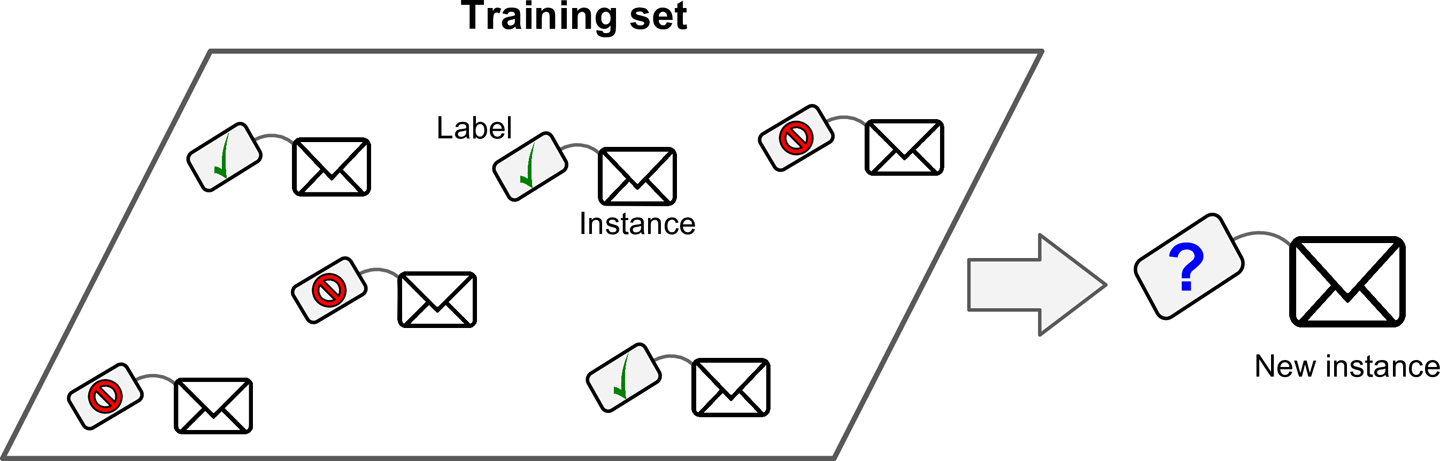
\includegraphics[scale=0.3]{Supervised Learning (1)}
\caption{}\label{SupervisedLearning1}
\end{figure}

Another typical task is to predict a \emph{target} numeric value, given a set of \emph{features}\footnote{In machine learning an attribute is a data type, while a feature has several meanings depending on the context, but
generally means an attribute plus its value. Many people use the words attribute and feature interchangeably, though.} called \emph{predictors}. This sort of task is called \emph{regression} because we start with an initial sample and the algorithm tries to extrapolate (Fig.~\ref{SupervisedLearning2}).
\begin{figure}[h!t]
\centering
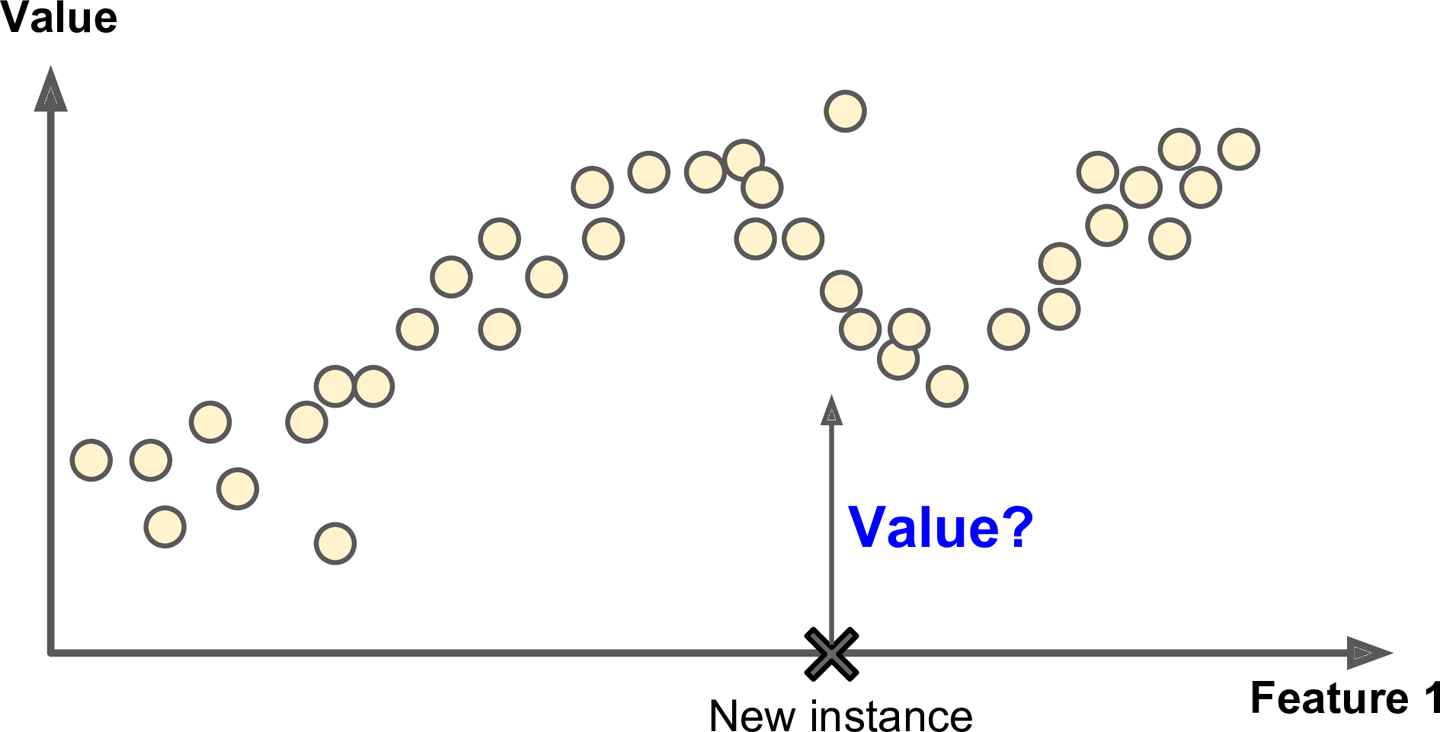
\includegraphics[scale=0.26]{Supervised Learning (2)}
\caption{}\label{SupervisedLearning2}
\end{figure}
%like neural networks
\subsubsection{Unsupervised learning}
In \textbf{unsupervised learning}, as you might guess, the training data is unlabeled. The system tries to learn without a teacher.

For example, say you have a lot of data about your blog’s visitors. You may want to run a \emph{clustering} algorithm to try to detect groups of similar visitors (Fig.~\ref{UnsupervisedLearning1}). At no point do you tell the algorithm which group a visitor belongs to: it finds those connections without your help. For example, it might notice that \SI{40}{\percent} of your visitors are males who love comic books, while \SI{20}{\percent} are young sci-fi lovers, and so on. If you use a \emph{hierarchical clustering} algorithm, it may also subdivide each group into smaller groups.
\begin{figure}[h!t]
\centering
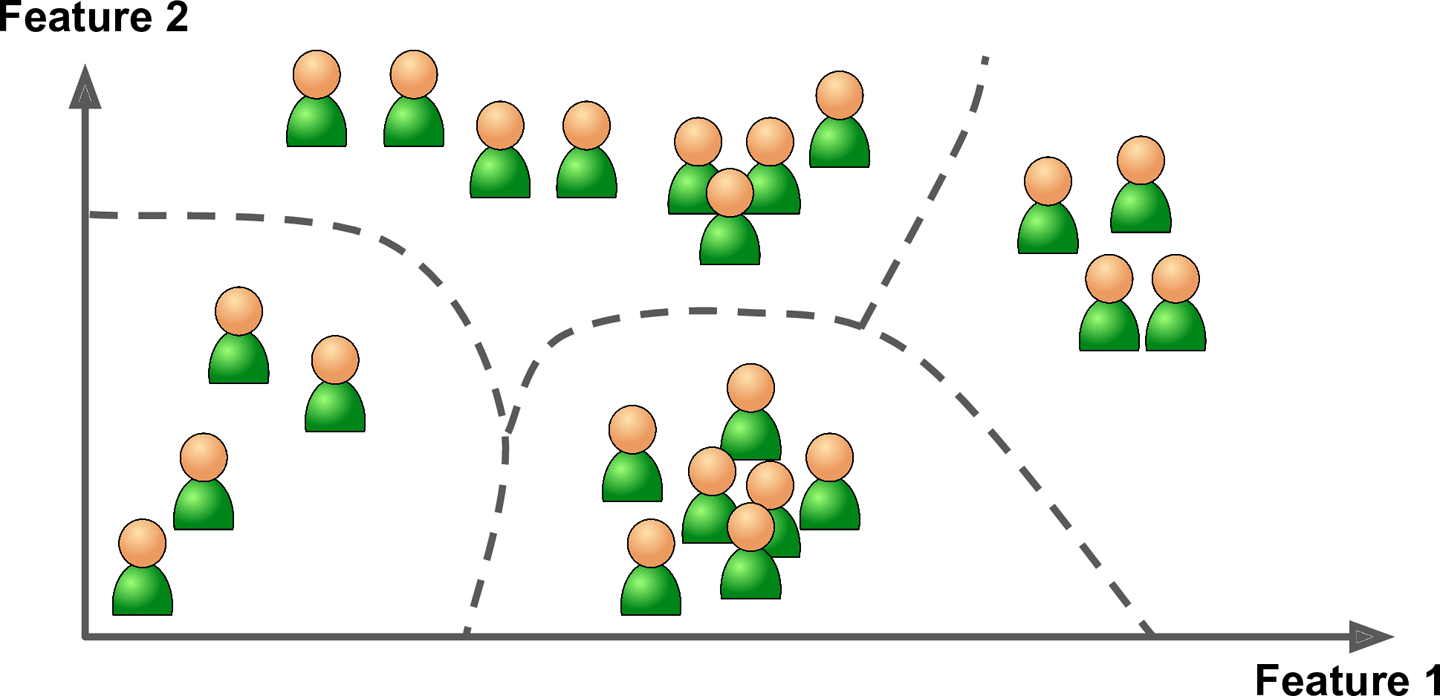
\includegraphics[scale=0.265]{Unsupervised Learning (1)}
\caption{}\label{UnsupervisedLearning1}
\end{figure}

Another important unsupervised task is \emph{anomaly detection}. The system is trained with normal instances, and when it sees a new instance it can tell whether it looks like a normal one or whether it is likely an anomaly. This happens, for example, in detecting unusual credit card transactions to prevent fraud, catching manufacturing defects, or automatically removing outliers from a dataset before feeding it to another learning algorithm.
\begin{figure}[h!t]
\centering
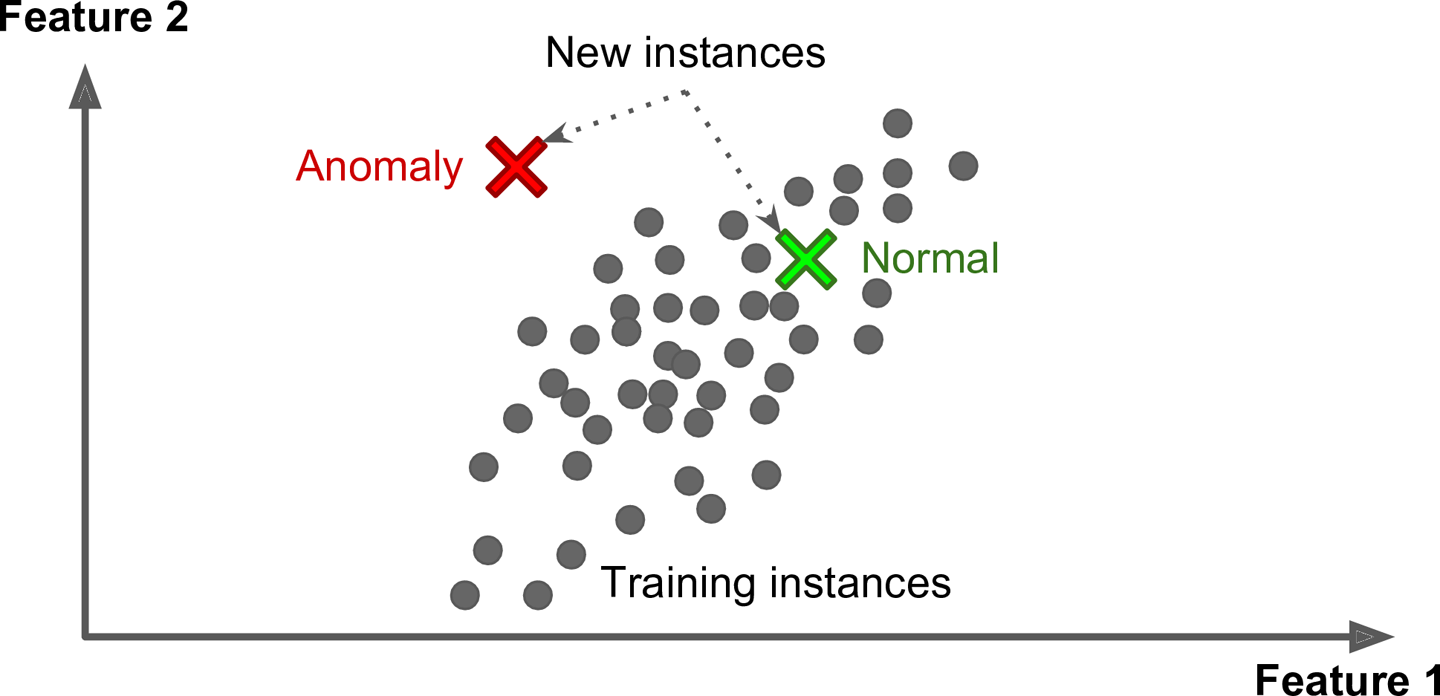
\includegraphics[scale=0.265]{Unsupervised Learning (2)}
\caption{}\label{UnsupervisedLearning2}
\end{figure}
\subsubsection{Semisupervised learning}
Some algorithms can deal with partially labeled training data, usually a lot of unlabeled data and a little bit of labeled data. This is called \textbf{semisupervised learning}.

Some photo-hosting services, such as Google Photos, are good examples of this. Once you upload all your family photos to the service, it automatically recognizes that the same person A shows up in photos 1, 5 and 11, while another person B shows up in photos 2, 5 and 7. This is the unsupervised part of the algorithm (clustering). Now all
the system needs is for you to tell it who these people are. Just one label per person in a single photo, and it is able to name everyone in every photo, which is useful for searching photos.

The unsupervised character of the learning is the clustering procedure. Consider for instance the situation depicted in Fig.~\ref{SemisupervisedLearning}. Triangles and squares represent the training set the algorithm has learned from, while the little gray circles are the new data that the algorithm has managed to group into clusters (some closer to triangles, others to squares). Now, suppose that the data indicated with a cross is presented to the system; by proximity it would seem closer to the squares than to the triangles of the training set. However, since the algorithm contains some unsupervised learning, it is able to recognize that the cross appears to be more likely to belong to the data cluster around the triangles. Therefore the system will be more inclined to categorize the cross on the same plane as the triangles.
\begin{figure}[h!t]
\centering
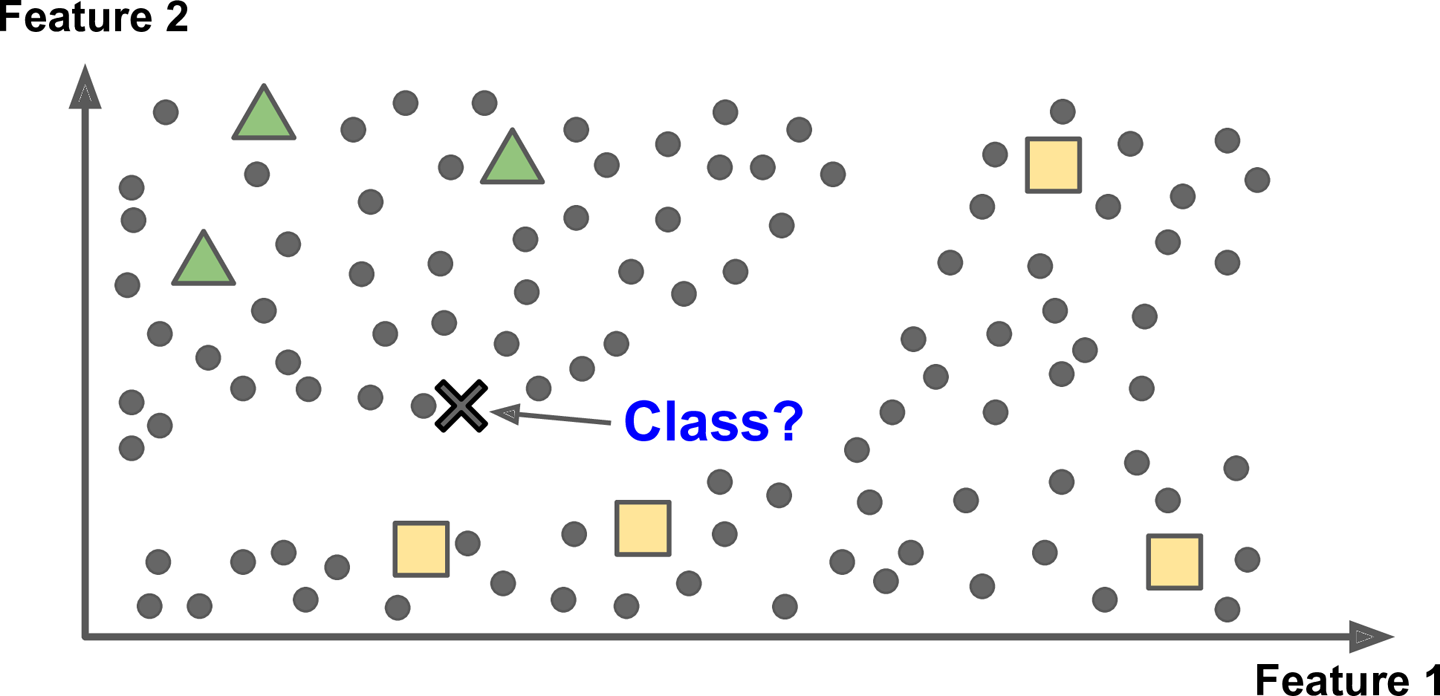
\includegraphics[scale=0.265]{Semisupervised Learning}
\caption{}\label{SemisupervisedLearning}
\end{figure}
\subsubsection{Reinforcement learning}
\textbf{Reinforcement learning} is a very different beast. The learning system, called an agent in this context, can observe the environment, select and perform actions, and get rewards in return (or penalties in the form of negative rewards, as in Figure~\ref{ReinforcementLearning}). It must then learn by itself what is the best strategy, called a policy, to get the most reward over time. A policy defines what action the agent should choose when it is in a given situation.
\begin{figure}[h!t]
\centering
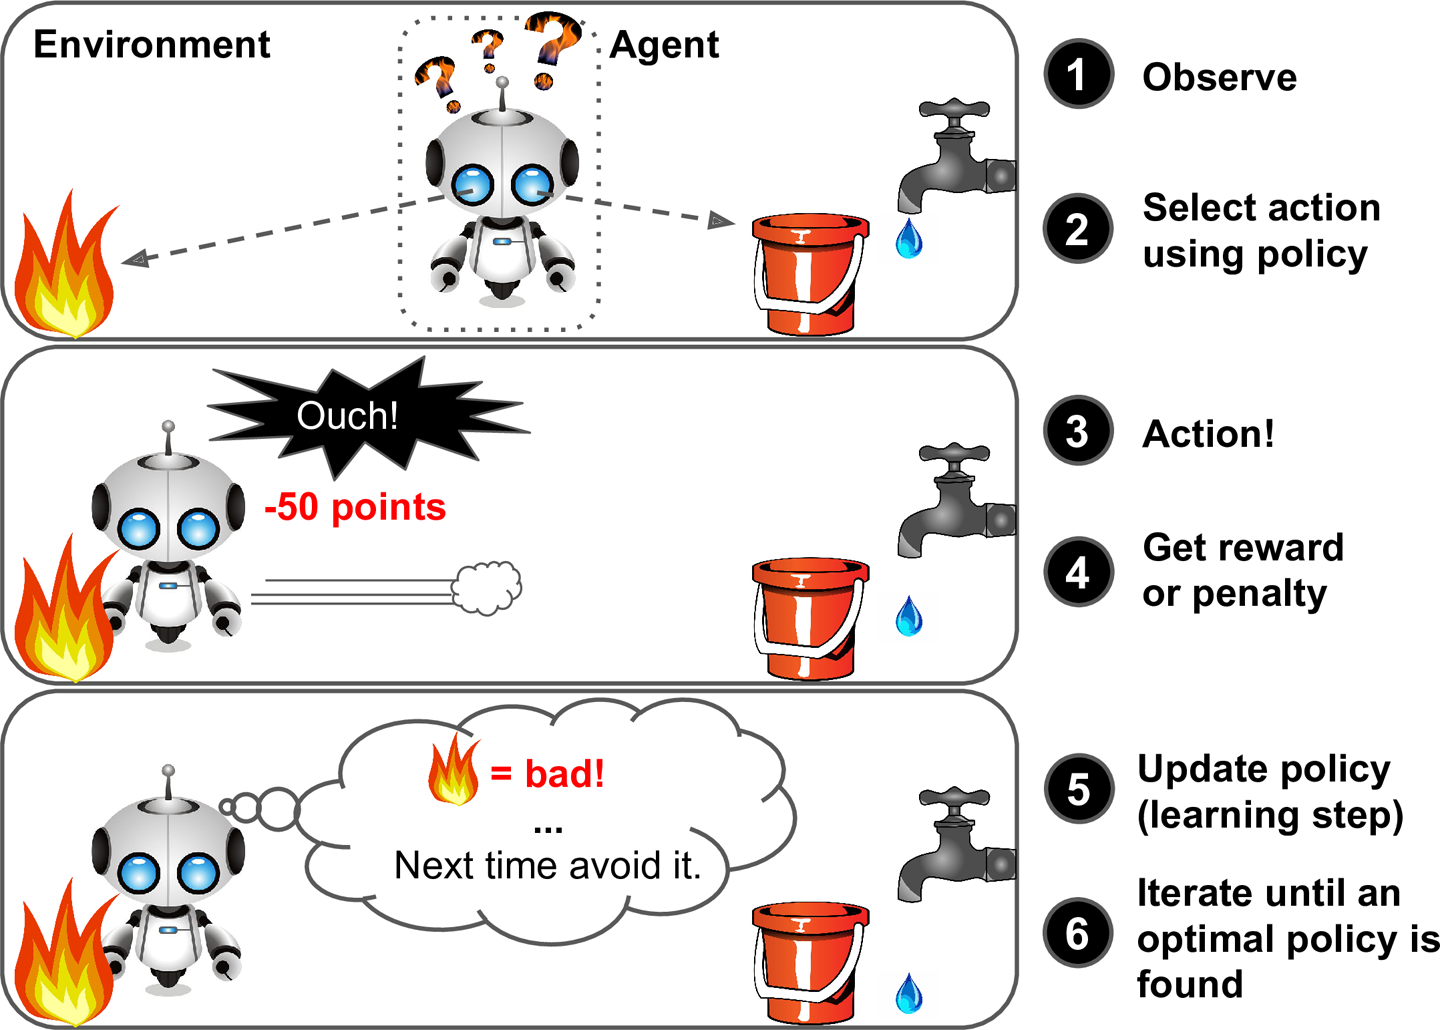
\includegraphics[scale=0.265]{Reinforcement Learning}
\caption{}\label{ReinforcementLearning}
\end{figure}

For example, many robots implement reinforcement learning algorithms to learn how to walk. DeepMind's AlphaGo program is also a good example of reinforcement learning applied to the game of go. It learned its winning policy by analyzing millions of games, and then playing many games against itself.
\subsection{Batch and online learning}
Another criterion used to classify machine learning systems is whether or not the system can learn incrementally from a stream of incoming data.
\subsubsection{Batch learning}
In \textbf{batch learning}, the system is incapable of learning incrementally: it must be trained using all the available data. This will generally take a lot of time and computing resources, so it is typically done offline. First the system is trained, and then it is launched into production and runs without learning anymore; it just applies what it has learned. This is called \emph{offline learning}.

If you want a batch learning system to know about new data (such as a new type of spam), you need to train a new version of the system from scratch on the full dataset (not just the new data, but also the old data), then stop the old system and replace it with the new one.
\subsubsection{Online learning}
In \textbf{online learning}, you train the system incrementally by feeding it data instances sequentially, either individually or by small groups called \emph{mini-batches}. Each learning step is fast and cheap, so the system can learn about new data on the fly, as they arrive (Fig.~\ref{OnlineLearning}).
\begin{figure}[h!t]
\centering
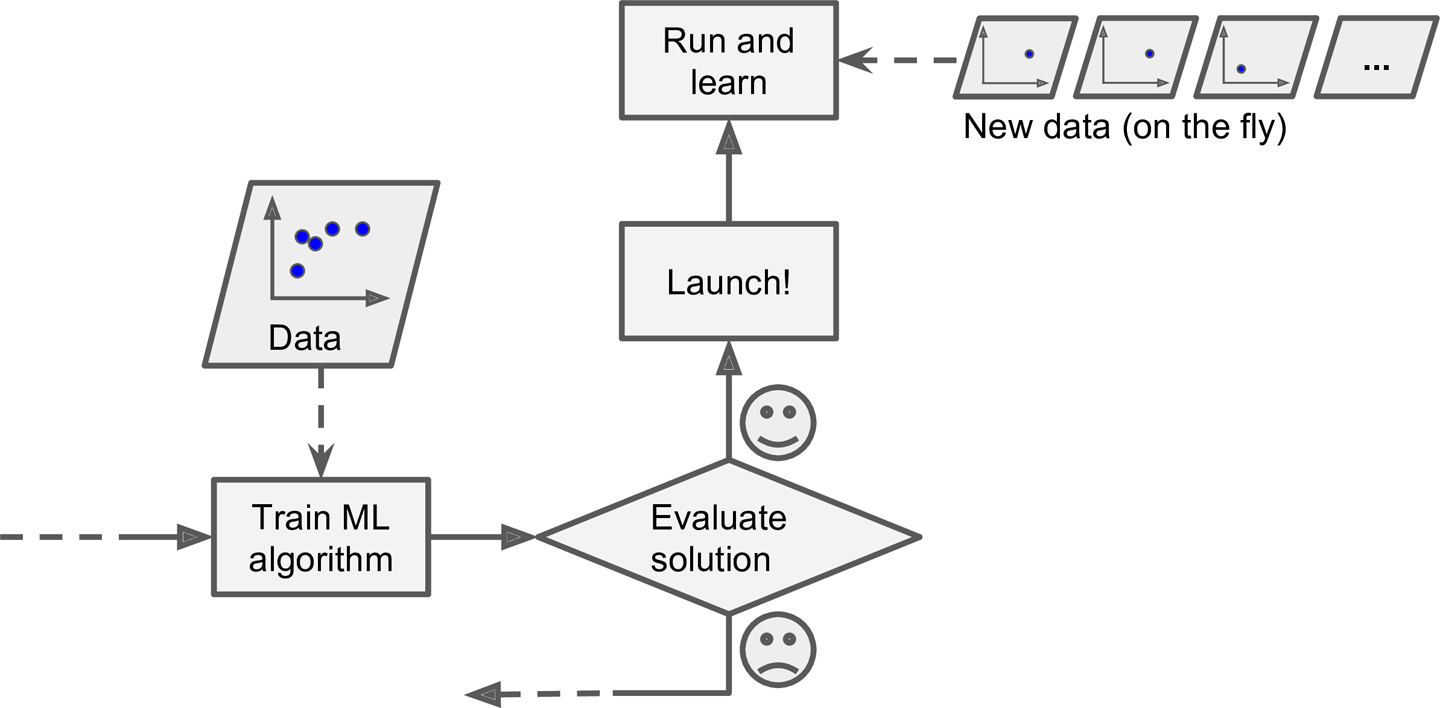
\includegraphics[scale=0.275]{Online Learning}
\caption{}\label{OnlineLearning}
\end{figure}

Online learning is great for systems that receive data as a continuous flow and need to adapt to change rapidly or autonomously. It is also a good option if you have limited computing resources: once an online learning system has learned about new data instances, it does not need them anymore, so you can discard them. This can save a huge amount of space.

Online learning algorithms can also be used to train systems on huge datasets that cannot fit in one machine's main memory (this is called \emph{out-of-core} learning). The algorithm loads part of the data, runs a training step on that data, and repeats the process until it has run on all of the data.

One important parameter of online learning systems is how fast they should adapt to changing data: this is called the \emph{learning rate}. If you set a high learning rate, then your system will rapidly adapt to new data, but it will also tend to quickly forget the old data (you don't want a spam filter to flag only the latest kinds of spam it was shown). Conversely, if you set a low learning rate, the system will have more inertia; that is, it will learn more slowly, but it will also be less sensitive to noise in the new data or to sequences of nonrepresentative data points.
\subsection{Instance-based and model-based learning}
One more way to categorize machine learning systems is by how they \emph{generalize}. Most machine learning tasks are about making predictions. This means that given a number of training examples, the system needs to be able to generalize to examples it has never seen before. Having a good performance measure on the training data is
good, but insufficient; the true goal is to perform well on new instances. There are two main approaches to generalization: instance-based learning and model-based learning.
\subsubsection{Instance-based learning}
Possibly the most trivial form of learning is simply to learn by heart. If you were to create a spam filter this way, it would just flag all emails that are identical to emails that have already been flagged by users—not the worst solution, but certainly not the best. Instead of just flagging emails that are identical to known spam emails, your spam filter could be programmed to also flag emails that are very similar to known spam emails. This requires a \emph{measure of similarity} between two emails. A (very basic) similarity measure between two emails could be to count the number of words they have in common. The system would flag an email as spam if it has many words in common with a known spam email. This is called \textbf{instance-based learning}: the system learns the examples by heart, then generalizes to new cases using a similarity measure.
\subsubsection{Model-based learning}
Another way to generalize from a set of examples is to build a model of these examples, then use that model to make predictions. In this way, when the system encounters new data, it does not try to detect similarity or proximity to the other examples it has learned; rather it categorizes the new element based on a well-defined model. For example, we can choose that all the data that falls within the dotted line in Fig.~\ref{Model-BasedLearning} are always classified as triangles, while the others as squares. This is called \textbf{model-based learning}.
\begin{figure}[h!t]
\centering
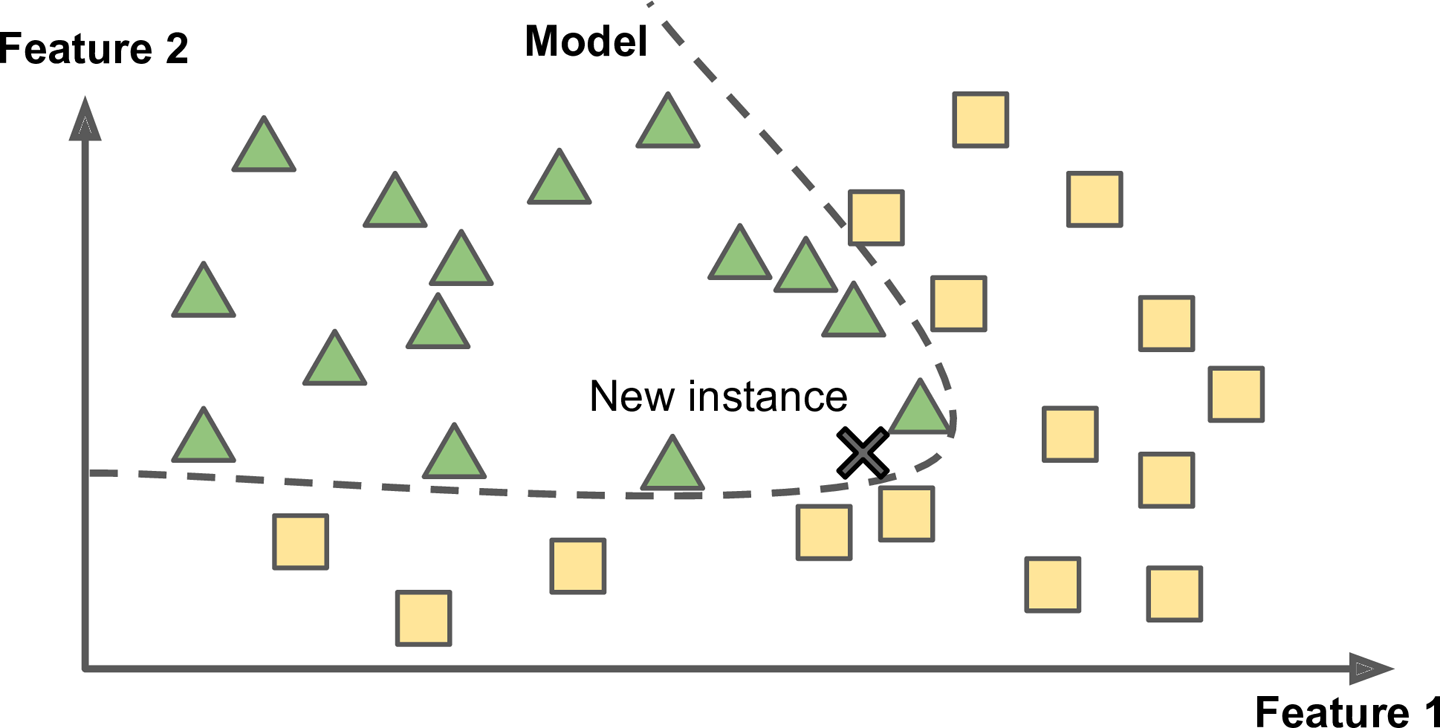
\includegraphics[scale=0.265]{Model-Based Learning}
\caption{}\label{Model-BasedLearning}
\end{figure}
\section{Testing and validating}\label{sec:Testing_and_validating}
In a famous paper published in 2001, some Microsoft researchers showed that very different machine learning algorithms, including fairly simple ones, performed almost identically well on a complex problem of natural language disambiguation once they were given enough data. As the authors put it: ``these results suggest that we may want to reconsider the tradeoff between spending time and money on algorithm development versus spending it on corpus development.'' In other words, \emph{data matters more than algorithms for complex problems}; typically, when we have huge amounts of data, the size of the dataset is dominant over the specific choice of the algorithm, which becomes essentially insignificant. It should be noted, however, that small- and medium-sized datasets are still very common, and it is not always easy or cheap to get extra training data, so don't abandon algorithms just yet.

In previous chapters we have often referred to the fact that a good machine, once properly instructed, is also able to generalize when it encounters ``unexpected'' instances. The only way to know how well a model will generalize to new cases is to actually try it out on new cases. One way to do that is to to split your data into two sets: the \textbf{training set} and the \textbf{test set}. As these names suggest, you train your model using the training set (in order to fix the parameters), and you test it using the test set. The error rate on new cases is called the \emph{generalization error}, and by evaluating your model on the test set, you get an estimation of this error. This value tells you how well your model will perform on instances it has never seen before.

If the training error is low (i.e., your model makes few mistakes on the training set) but the generalization error is high, it means that your model is \emph{overfitting} the training data. This means that the machine will work almost perfectly on the training set, and only on this, but it will almost always fail in generalizing. Overfitting typically occurs when we try to learn the training set with a model having many degrees of freedom; e.g., when we have a sample of $N$ points and we decide to describe the distribution by fitting the data with a polynomial of order $N-1$ (cf. interpolation in Sec.~\ref{sec:Generalizationandfitting}).
Instead, as you might guess, \emph{underfitting} is the opposite of overfitting: it occurs when your model is too simple to learn the underlying structure of the data. Reality is just more complex than the model, so its predictions are bound to be inaccurate, even on the training examples.
Of course, the crucial point is to find the right balance between fitting the data perfectly and keeping the model simple enough to ensure that it will generalize well.

Constraining a model to make it simpler and reduce the risk of overfitting is called \emph{regularization} (N.B.: constraining, not reducing the degrees of freedom!). The amount of regularization to apply during learning can be controlled by a \textbf{hyperparameter}. A hyperparameter is a parameter defining a learning algorithm (not a model). As such, it is not affected by the learning algorithm itself; it must be set prior to training and remains constant during training. Examples of hyperparameters are, for example:
\begin{itemize}
\item the topology and size of a neural networks (recall that in the previous chapter we did not say what was the optimal number of layers and hidden neurons for the percepetron);
\item the parameter $\varepsilon$ in the gradient method;
\item the learning rate;
\item the mini-batch size.
\end{itemize}
If you set the regularization hyperparameter to a very large value, you will get an almost flat model; the learning algorithm will almost certainly not overfit the training data, but it will be less likely to find a good solution. Tuning hyperparameters is an important part of building a machine learning system.

So evaluating a model is simple enough: just use a test set. Now suppose you are hesitating between two models (say a linear model and a polynomial model): how can you decide? One option is to train both and compare how well they generalize using the test set. Now suppose that the linear model generalizes better, but you want to apply some regularization to avoid overfitting. The question is: how do you choose the value of the regularization hyperparameter?

%A common solution to this problem is to have a second holdout set called the \emph{validation set}. First you train multiple models with various hyperparameters using the training set and you test them on the validation set. Then you select the model and hyperparameters that perform best on the validation set and you train it on the whole ``learning set'', i.e. training set plus validation set. Finally, when you're happy with your model you run a single final test against the test set to get an estimate of the generalization error.
A common solution to this problem is to have a second holdout set: you simply hold out part of the training set to evaluate several candidate models and select the best one. The new held-out set is called the \textbf{validation set}. More specifically, you train multiple models with various hyperparameters on the \textbf{reduced training set} (i.e., the full training set minus the validation set), and you select the model that performs best on the validation set. After this holdout validation process, you train the best model on the full training set (including the validation set), and this gives you the final model. Lastly, you evaluate this final model on the test set to get an estimate of the generalization error.

This solution usually works quite well. However, if the validation set is too small, then model evaluations will be imprecise: you may end up selecting a suboptimal model by mistake. Conversely, if the validation set is too large, then the remaining training set will be much smaller than the full training set. Why is this bad? Well, since the final model will be trained on the full training set, it is not ideal to compare candidate models trained on a much smaller training set. One way to solve this problem is to perform repeated \textbf{cross-validation}, using many small validation sets. A training dataset can be repeatedly split up into a reduced training dataset and a validation dataset. These repeated partitions can be done in various ways, such as dividing into two equal datasets and using them as training/validation, and then validation/training, or repeatedly selecting a random subset as a validation dataset. Each model is evaluated once per validation set after it is trained on the rest of the data. By averaging out all the evaluations of a model, you get a much more accurate measure of its performance. There is a drawback, however: the training time is multiplied by the number of validation sets.
\section{Quality of data and preprocessing}
In some cases, it's easy to get a large amount of data for training, but this data probably won't be perfectly representative of the data that will be used in production. In this case, the most important rule to remember is that the validation set and the test set must be as \emph{representative} as possible of the data you expect to use in production, i.e. representative of the new cases you want to generalize to.

Another thing which can go wrong in machine learning projects is to have poor-quality data. Obviously, if your training data is full of errors, outliers, and noise (e.g., due to poor-quality measurements), it will make it harder for the system to detect the underlying patterns, so your system is less likely to perform well. It is often well worth the effort to spend time \emph{cleaning up your training data}. The truth is, most data scientists spend a significant part of their time doing just that.

Your system will only be capable of learning if the training data contains enough relevant features and not too many irrelevant ones. A critical part of the success of a machine learning project is coming up with a good set of features to train on. This process, called \emph{feature engineering}, involves the following steps.
\begin{itemize}
\item \emph{Feature selection}: selecting the most useful features to train on among existing features;
\item \emph{Feature extraction}: combining existing features to produce a more useful one—as we saw earlier, dimensionality reduction algorithms can help;
\item Creating new features by gathering new data.
\end{itemize}
In summary, before feeding the machine with data to train on, it is necessary to practice the necessary amount of \emph{preprocessing}, in order to reduce the data mismatch.
\section{California housing prices}\label{sec:Californiahousingprices}
When you are learning about machine learning, it is best to experiment with real-world data, not artificial datasets. Fortunately, there are thousands of open datasets to choose from, ranging across all sorts of domains. In this section we'll use the California Housing Prices dataset from the StatLib repository. This dataset is based on data from the 1990 California census. It is not exactly recent (a nice house in the Bay Area was still affordable at the time), but it has many qualities for learning, so we will pretend it is recent data. For teaching purposes we've added a categorical attribute and removed a few features.

Our first task is to use California census data to build a model of housing prices in the state. This data includes metrics such as the population, median income and median housing price for each block group in California. Block groups are the smallest geographical unit for which the US Census Bureau publishes sample data (a block group typically has a population of \num{600} to \num{3000} people). We will call them ``districts'' for short.
\subsection{Frame the problem}
With all this information, you are now ready to start designing your system. First, you need to frame the problem: is it supervised, unsupervised or reinforcement learning? Is it a classification task, a regression task or something else? Should you use batch learning or online learning techniques? Let's see: it is clearly a typical supervised learning task, since you are given \emph{labeled} training examples (each instance comes with the expected output, i.e., the district's median housing price). It is also a typical regression task, since you are asked to predict a value (the price). More specifically, this is a \emph{multiple regression} problem, since the system will use multiple features to make a prediction (it will use the district's population, the median income, etc.). It is also a \emph{univariate regression} problem, since we are only trying to predict a single value for each district. If we were trying to predict multiple values per district, it would be a \emph{multivariate regression} problem. Finally, there is no continuous flow of data coming into the system, there is no particular need to adjust to changing data rapidly, and the data is small enough to fit in memory, so plain batch learning should do just fine.
\subsection{Select a performance measure}
The first step is to select a performance measure. A typical performance measure for regression problems is the \textbf{root-mean-square-error} (RMSE). It gives an idea of how much error the system typically makes in its predictions, with a higher weight for large errors. Equation \eqref{RMSE} shows the mathematical formula to compute the RMSE:
\begin{equation}\label{RMSE}
\operatorname{RMSE}\s(\mathbf{X},h)=\sqrt{\frac{1}{m}\sum_{i=1}^m{\Bigl[h\bigl(\mathbf{x}^{(i)}\bigr)-y^{(i)}\Bigr]}^2}
\end{equation}
This equation introduces several very common machine learning notations that we will use throughout this book.
\begin{itemize}
\item $m$ is the number of instances in the dataset you are measuring the RMSE on (e.g. the total number of districts).
\item $\mathbf{x}^{(i)}$ is a vector of all the feature values (excluding the label) of the $i$-th instance in the dataset, and $y^{(i)}$ is its label (the desired output value for that instance). For example, if the first district in the dataset is located at longitude \ang{-118.29}, latitude \ang{33.91}, and it has \num{1416} inhabitants with a median income of \SI{38372}[\$\,]{}, and the median house value is \SI{156400}[\$\,]{} (ignoring the other
features for now), then
\begin{equation}
\mathbf{x}^{(1)}=\begin{pmatrix}
-118.29\\
33.91\\
\num{1416}\\
\num{38372}
\end{pmatrix}
\end{equation}
and
\begin{equation}
y^{(1)}=\num{156400}
\end{equation}
\item $\mathbf{X}$ is a matrix containing all the feature values (excluding labels) of all instances in the dataset. There is one row per instance, and the $i$-th row is equal to the transpose of $\mathbf{x}^{(i)}$, noted ${\bigl(\mathbf{x}^{(i)}\bigr)}^{\mathrm{T}}$.
\begin{equation}
\mathbf{X}=\begin{pmatrix}
{\bigl(\mathbf{x}^{(1)}\bigr)}^{\mathrm{T}}\\
{\bigl(\mathbf{x}^{(2)}\bigr)}^{\mathrm{T}}\\
\vdots\\
{\bigl(\mathbf{x}^{(m)}\bigr)}^{\mathrm{T}}
\end{pmatrix}=\begin{pmatrix}
-118.29 & 33.91 & \num{1416} & \num{38372} \\
\vdots & \vdots & \vdots & \vdots
\end{pmatrix}
\end{equation}
\item $h$ is your system's prediction function, also called a \emph{hypothesis}. When your system is given an instance's feature vector $\mathbf{x}^{(i)}$, it outputs a predicted value $\widehat{y}^{(i)}=h\bigl(\mathbf{x}^{(i)}\bigr)$ for that instance. For example, if your system predicts that the median housing price in the first district is \SI{156400}[\$\,]{}, then $\widehat{y}^{(1)}=h\bigl(\mathbf{x}^{(1)}\bigr)=\num{156400}$.
\end{itemize}

Even though the RMSE is generally the preferred performance measure for regression tasks, in some contexts you may prefer to use another function. For example, suppose that there are many outlier districts. In that case, you may consider using the \textbf{mean absolute error} (MAE, also called the average absolute deviation):
\begin{equation}\label{MAE}
\operatorname{MAE}\s(\mathbf{X},h)=\frac{1}{m}\sum_{i=1}^m\Bigl\lvert h\bigl(\mathbf{x}^{(i)}\bigr)-y^{(i)}\Bigr\rvert
\end{equation}

Both the RMSE and the MAE are ways to measure the distance between two vectors: the vector of predictions and the vector of target values. Various distance measures, or \emph{norms}, are possible:
\begin{equation}\label{norm}
\operatorname{Error}\s(\mathbf{X},h)={\left[\frac{1}{m}\sum_{i=1}^m{\Bigl\lvert h\bigl(\mathbf{x}^{(i)}\bigr)-y^{(i)}\Bigr\rvert}^k\right]}^{1/k}
\end{equation}
The higher the norm index $k$, the more it focuses on large values and neglects small ones. This is why the RMSE is more sensitive to outliers than the MAE. But when outliers are exponentially rare (like in a bell-shaped curve), the RMSE performs very well and is generally preferred.
\subsection{Get the data}
First you will need to have Python installed. You will also need a number of Python modules: Jupyter, NumPy, pandas, Matplotlib and Scikit-Learn. A valid alternative to installing Python and related packages is Google Colab, which allows you to write and run Python code online in your browser without any configuration (however, this will inevitably increase the compilation time). For the code refer to the attached notebook \attachfile[icon=CustomPushPin,modified=20210422120528+01'00',size=1330086]{Attachments/02_end_to_end_machine_learning_project.ipynb}.

In the first few lines we have essentially imported all the packages and downloaded the data from the online database. Now let's load the data using pandas. Once again, you should write a small function to load the data (\jupytercode{load\_housing\_data}). This function returns a pandas DataFrame object containing all the data. Let's take a look at the top five rows using the DataFrame's \jupytercode{head()} method (Fig.~\ref{02_[5]_Out}). Each row represents one district. There are 10 attributes: \jupytercode{longitude}, \jupytercode{latitude}, \jupytercode{housing\_median\_age}, \jupytercode{total\_rooms}, \jupytercode{total\_bedrooms} (the latter two are the total in all the district, not in a single house), \jupytercode{population}, \jupytercode{households}, \jupytercode{median\_income}, \jupytercode{median\_house\_value} and \jupytercode{ocean\_proximity}.
\begin{figure}[h!t]
\centering
\vspace{1pt}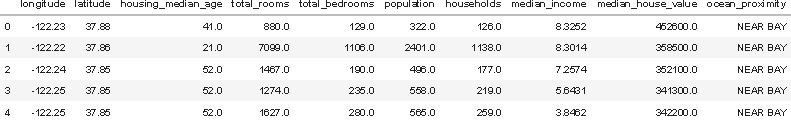
\includegraphics[width=\textwidth]{02_[5]_Out}
\caption{\jupytercode[0.913]{In[5]: housing = load\_housing\_data()} $\hookleftarrow$ \jupytercode{housing.head()}.}\label{02_[5]_Out}
\end{figure}

The \jupytercode{info()} method is useful to get a quick description of the data, in particular the total number of rows, each attribute's type, and the number of non-null values (Fig.~\ref{02_[6]_In}).
\begin{figure}[h!t]
\centering
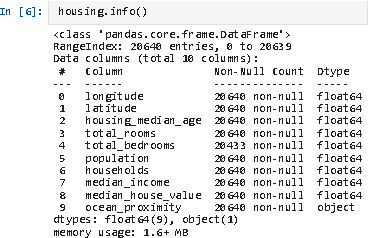
\includegraphics[scale=1.7000]{02_[6]_In}
\caption{}\label{02_[6]_In}
\end{figure}

All attributes are numerical, except the \jupytercode{ocean\_proximity} field. Its type is object, so it could hold any kind of Python object. But since you loaded this data from a CSV file, you know that it must be a text attribute. When you looked at the top five rows, you probably noticed that the values in the \jupytercode{ocean\_proximity} column were repetitive, which means that it is probably a categorical attribute. You can find out what categories exist and how many districts belong to each category by using the \jupytercode{value\_counts()} method (Fig.~\ref{02_[7]_In-Out}).
\begin{figure}[h!t]
\centering
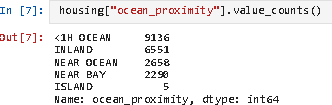
\includegraphics[scale=1.7000]{02_[7]_In-Out}
\caption{}\label{02_[7]_In-Out}
\end{figure}

Let’s look at the other fields. The \jupytercode{describe()} method shows a summary of the numerical attributes (Fig.~\ref{02_[8]_Out}). The \jupytercode{count}, \jupytercode{mean}, \jupytercode{min} and \jupytercode{max} rows are self-explanatory. Note that the null values are ignored (so, for example, the count of \jupytercode{total\_bedrooms} is \num{20433}, not \num{20640}). The \jupytercode{std} row shows the standard deviation, which measures how
dispersed the values are. The \jupytercode{25\%}, \jupytercode{50\%} and \jupytercode{75\%} rows show the corresponding \emph{percentiles}: a percentile indicates the value below which a given percentage of observations in a group of observations fall. For example, \SI{25}{\percent} of the districts have a \jupytercode{housing\_median\_age} lower than 18, while \SI{50}{\percent} are lower than 29 and \SI{75}{\percent} are lower than 37. These are often called the 25-th percentile (or first quartile), the median, and the 75-th percentile (or third quartile).
\begin{figure}[h!t]
\centering
\vspace{1pt}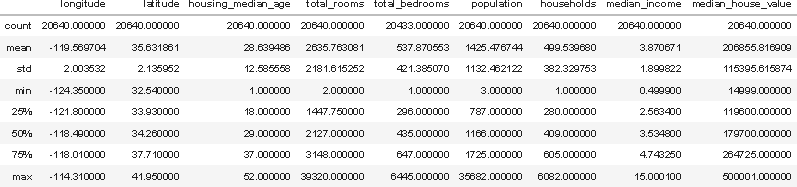
\includegraphics[width=\textwidth]{02_[8]_Out}
\caption{\jupytercode[0.913]{In[8]: housing.describe()}.}\label{02_[8]_Out}
\end{figure}

Another quick way to get a feel of the type of data you are dealing with is to plot a histogram for each numerical attribute. A histogram shows the number of instances (on the vertical axis) that have a given value range (on the horizontal axis). You can either plot this one attribute at a time, or you can call the \jupytercode{hist()} method on the whole dataset, and it will plot a histogram for each numerical attribute (Fig.~\ref{02_[9]_In}).
\begin{figure}[h!t]
\centering
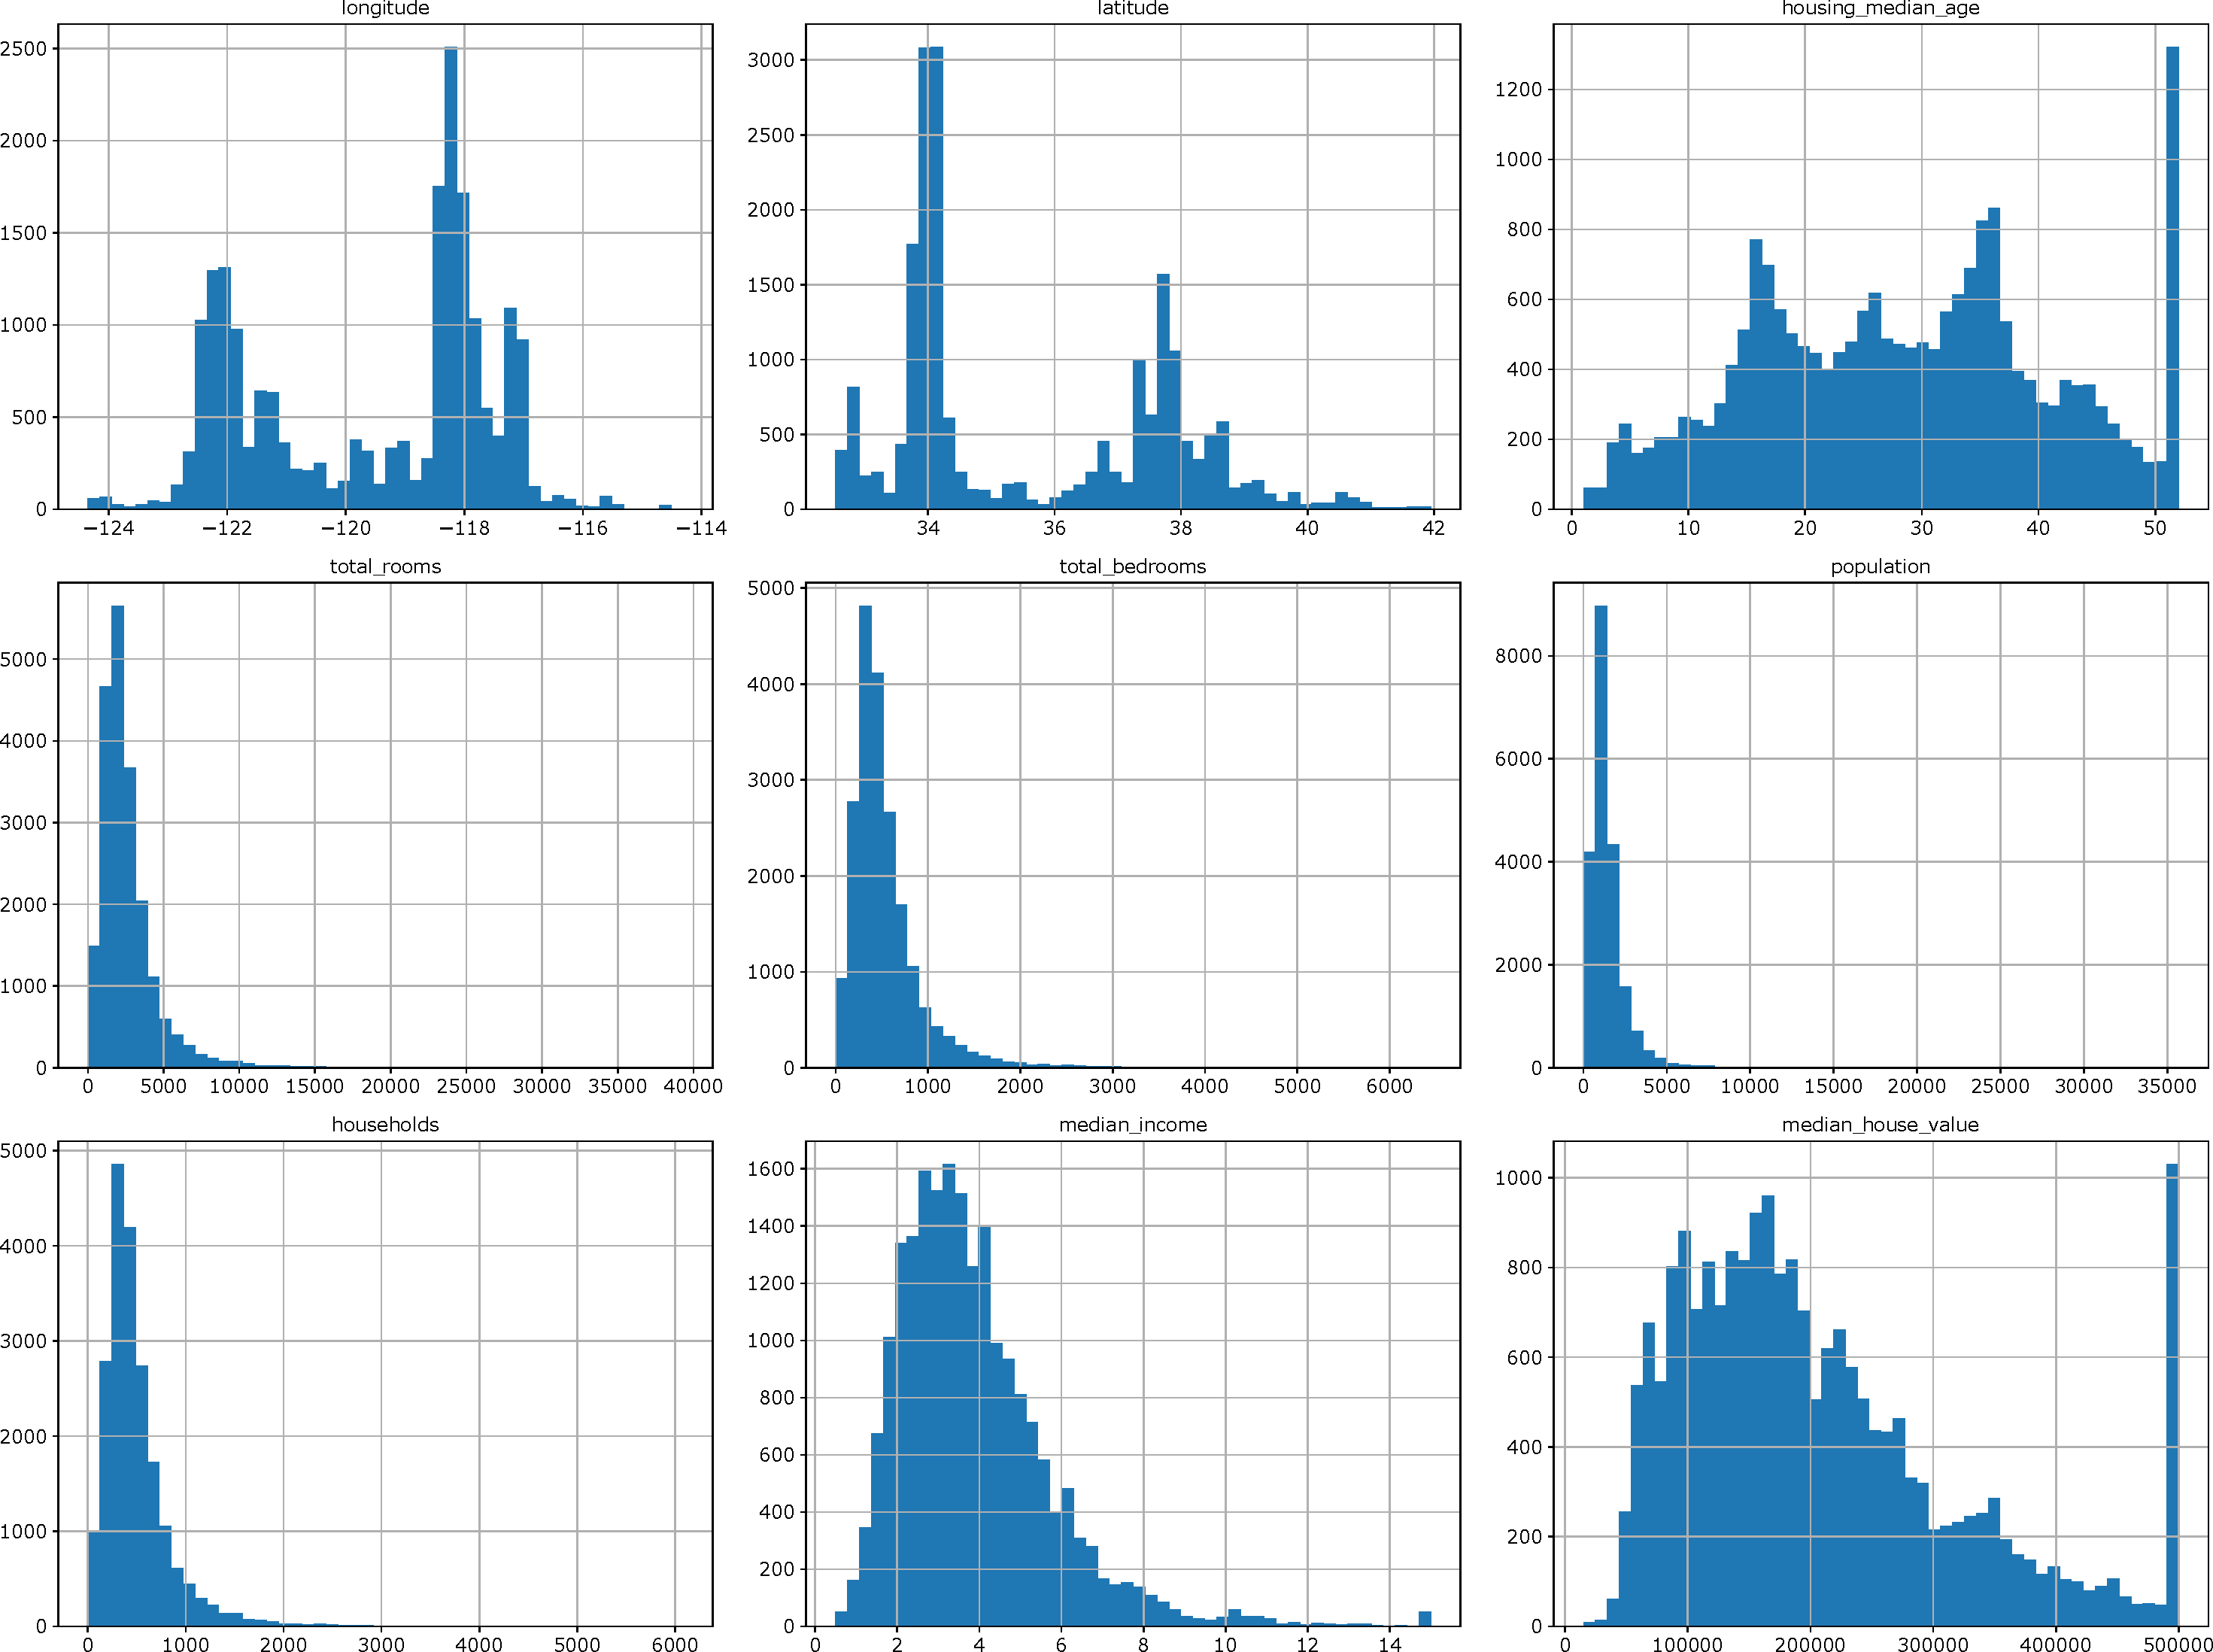
\includegraphics[width=\textwidth]{02_[9]_In}
\caption{\jupytercode[0.913]{In[9]: housing.hist(bins=50, figsize=(20,15))}.}\label{02_[9]_In}
\end{figure}

There are a few things you might notice in these histograms:
\begin{itemize}
\item First, the median income attribute does not look like it is expressed in US dollars (USD). After checking with the team that collected the data, you are told that the data has been scaled and capped at 15 (actually, 15.0001) for higher median incomes, and at 0.5 (actually, 0.4999) for lower median incomes. The numbers represent roughly
tens of thousands of dollars (e.g., 3 actually means about \SI{30000}[\$\,]{}).
%Working with preprocessed attributes is common in machine learning, and it is not necessarily a problem, but you should try to understand how the data was computed.
\item The housing median age and the median house value were also capped. The latter may be a serious problem since it is your target attribute (your labels). Your machine learning algorithms may learn that prices never go beyond that limit. You need to check with your client team (the team that will use your system's output) to see if this is a problem or not.
\item These attributes have very different scales. We will discuss this later, when we explore feature scaling.
\item Finally, many histograms are tail-heavy: they extend much farther to the right of the median than to the left. This may make it a bit harder for some machine learning algorithms to detect patterns. We will try transforming these attributes later on to have more bell-shaped distributions.
\end{itemize}
\subsection{Create a test set}
At this point we have to train the machine, that is, we have to create a test set, put it aside and never look at it. Creating a test set is theoretically simple: pick some instances randomly, typically \SI{20}{\percent} of the dataset, or less if your dataset is very large, and set them aside (\jupytercode{train\_set, test\_set = split\_train\_test(housing, 0.2)}). Well, this works, but it is not perfect: if you run the program again, it will generate a different test set! Over time, you (or your machine learning algorithms) will get to see the whole dataset, which is what you want to avoid. One solution is to save the test set on the first run and then load it in subsequent runs. Another option is to set the random number generator's seed (e.g., with \jupytercode{np.random.seed(42)}) before calling \jupytercode{np.random.permutation()} so that it always generates the same shuffled indices.

But both these solutions will break the next time you fetch an updated dataset. To have a stable train/test split even after updating the dataset, a common solution is to use each instance's identifier to decide whether or not it should go in the test set (assuming instances have a unique and immutable identifier). For example, you could compute a hash of each instance’s identifier and put that instance in the test set if the hash is lower than or equal to \SI{20}{\percent} of the maximum hash value. This ensures that the test set will remain consistent across multiple runs, even if you refresh the dataset. The new test set will contain \SI{20}{\percent} of the new instances, but it will not contain any instance that was previously in the training set. On line \jupytercode{In[14]} is a possible implementation. Unfortunately, the housing dataset does not have an identifier column. The simplest solution is to use the row index as the ID. If you use the row index as a unique identifier, you need to make sure that new data gets appended to the end of the dataset and that no row ever gets deleted. If this is not possible, then you can try to use the most stable features to build a unique identifier. For example, a district's latitude and longitude are guaranteed to be stable for a few million years, so you could combine them into an ID (see the following lines).

Scikit-Learn provides a few functions to split datasets into multiple subsets in various ways. The simplest function is \jupytercode{train\_test\_split()}, which does pretty much the same thing as the function \jupytercode{split\_train\_test()}, with a couple of additional features. First, there is a \jupytercode{random\_state} parameter that allows you to set the random generator seed. Second, you can pass it multiple datasets with an identical number of rows, and it will split them on the same indices (this is very useful, for example, if you have a separate DataFrame for labels).

So far we have considered purely random sampling methods. This is generally fine if your dataset is large enough (especially relative to the number of attributes), but if it is not, you run the risk of introducing a significant sampling bias. When a survey company decides to call \num{1000} people to ask them a few questions, they don't just pick \num{1000} people randomly in a phone book. They try to ensure that these \num{1000} people are representative of the whole population. For example, the US population is \SI{51.3}{\percent} females and \SI{48.7}{\percent} males, so a well-conducted survey in the US would try to maintain this ratio in the sample: 513 female and 487 male. This is called \emph{stratified sampling}: the population is divided into homogeneous subgroups called \emph{strata} (e.g. females and males), and the right number of instances are sampled from each stratum to guarantee that the test set is representative of the overall population (i.e. \SI{51.3}{\percent} and \SI{48.7}{\percent} respectively). If the people running the survey used purely random sampling from the whole population, there would be about a \SI{12}{\percent} chance of sampling a skewed test set that was either less than \SI{49}{\percent} female or more than \SI{54}{\percent} female. Either way, the survey results would be significantly biased.

Suppose you chatted with experts who told you that the median income is a very important attribute to predict median housing prices. You may want to ensure that the test set is representative of the various categories of incomes in the whole dataset. Since the median income is a continuous numerical attribute, you first need to create an income category attribute. Let's look at the median income histogram more closely (back in  Fig.~\ref{02_[9]_In}): most median income values are clustered around 1.5 to 6 (i.e., \$\,\numrange{15000}{60000}), but some median incomes go far beyond 6. It is important to have a sufficient number of instances in your dataset for each stratum, or else the estimate of a stratum's importance may be biased. This means that you should not have too many strata, and each stratum should be large enough. The code at line \jupytercode{In[23]} uses the \jupytercode{pd.cut()} function to create an income category attribute with five categories (labeled from 1 to 5): category 1 ranges from 0 to 1.5 (i.e., less than \SI{15000}[\$\,]{}), category 2 from 1.5 to 3, and so on. These income categories are represented in Figure~\ref{02_[24-25]_In-Out}.
\begin{figure}[h!t]
\centering
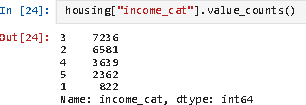
\includegraphics[scale=1.7000]{02_[24]_In-Out}

\vspace{\baselineskip}\noindent
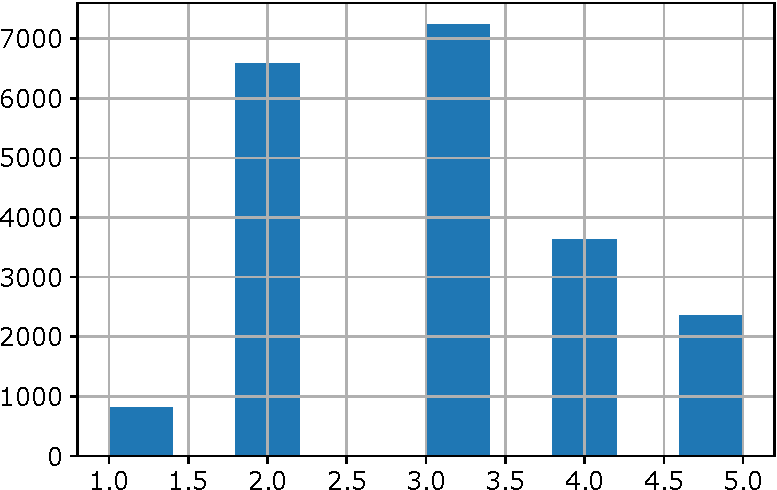
\includegraphics[scale=0.65]{02_[25]_Out}
\caption{\jupytercode[0.913]{In[25]: housing["income\_cat"].hist()}.}\label{02_[24-25]_In-Out}
\end{figure}

Now you are ready to do stratified sampling based on the income category. For this you can use Scikit-Learn's \jupytercode{StratifiedShuffleSplit} class (\jupytercode{In[26]}). Let's see if this worked as expected. You can start by looking at the income category proportions in the test set (Fig.~\ref{02_[27]_In-Out}).
\begin{figure}[h!t]
\centering
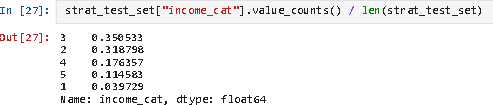
\includegraphics[scale=1.7000]{02_[27]_In-Out}
\caption{}\label{02_[27]_In-Out}
\end{figure}

With similar code you can measure the income category proportions in the full dataset, i.e. for data depicted in Figure~\ref{02_[24-25]_In-Out}. Finally, Figure~\ref{02_[30]_Out} compares the income category proportions in the overall dataset, in the test set generated with stratified sampling, and in a test set generated using purely random sampling. As you can see, the test set generated using stratified sampling has income category proportions almost identical to those in the full dataset, whereas the test set generated using purely random sampling is skewed. Note also that the error in the random sampling can become quite large (e.g. about \SI{5}{\percent}), while for the stratified sampling it remains very low.
\begin{figure}[h!t]
\centering
\vspace{1pt}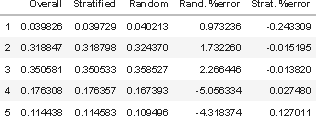
\includegraphics[scale=1.7]{02_[30]_Out}
%\texttt{In[30]: }\texttt{compare\_props}
\caption{Sampling bias comparison of stratified versus purely random sampling.}\label{02_[30]_Out}
\end{figure}

We spent quite a bit of time on test set generation for a good reason: this is an often neglected but critical part of a machine learning project. Moreover, many of these ideas will be useful later when we discuss cross-validation. Now it's time to move on to the next stage: exploring the data.
\subsection{Data visualization}
So far you have only taken a quick glance at the data to get a general understanding of the kind of data you are manipulating. Now the goal is to go into a little more depth. First, make sure you have put the test set aside and you are only exploring the training set. Also, if the training set is very large, you may want to sample an exploration set, to make manipulations easy and fast. In our case, the set is quite small, so you can just work directly on the full set. Let's create a copy so that you can play with it without harming the training set: \jupytercode{housing = strat\_train\_set.copy()}.

Since there is geographical information (latitude and longitude), it is a good idea to create a scatterplot of all districts to visualize the data (Fig.~\ref{02_[33]_In}).
\begin{figure}[h!t]
\centering
%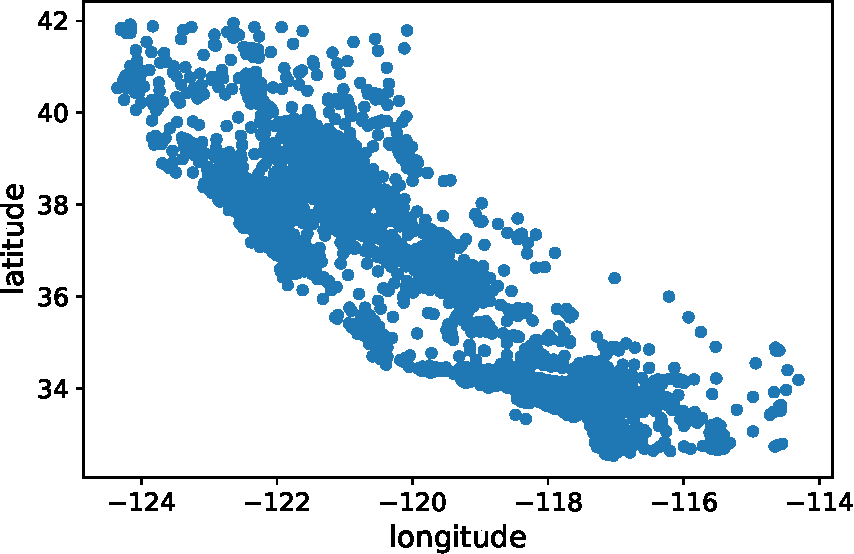
\includegraphics[scale=0.65]{02_[33]_In.pdf}
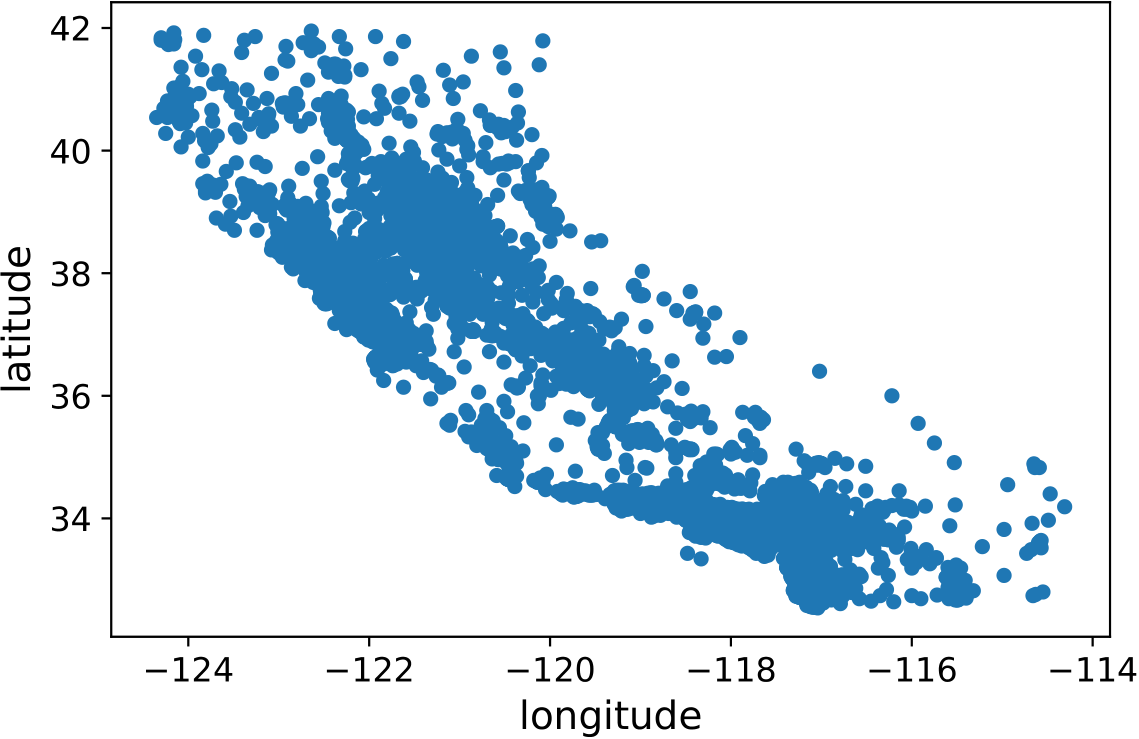
\includegraphics[scale=0.25]{02_[33]_In.png}
\caption{A geographical scatterplot of the data.}\label{02_[33]_In}
%\texttt{In[33]: }\texttt{housing.plot(kind="scatter", x="longitude", y="latitude")}.
\end{figure}

This looks like California all right, but other than that it is hard to see any particular pattern. Setting the \jupytercode{alpha} option to 0.1 (i.e. the transparency of the points) makes it much easier to visualize the places where there is a high density of data points. Now that's much better: you can clearly see the high-density areas, namely the Bay Area and around Los Angeles and San Diego, plus a long line of fairly high density in the Central Valley, in particular around Sacramento and Fresno (Fig.~\ref{02_[34]_In}). Our brains are very good at spotting patterns in pictures, but you may need to play around with visualization parameters to make the patterns stand out.
\begin{figure}[h!t]
\centering
%\includegraphics[scale=0.65]{02_[34]_In.pdf}
\includegraphics[scale=0.25]{02_[34]_In.png}
\caption{A better visualization that highlights high-density areas.}\label{02_[34]_In}
%\texttt{In[34]: }\texttt{housing.plot(kind="scatter", x="longitude", y="latitude", alpha=0.1)}.
\end{figure}

Now let's look at the housing prices (Fig.~\ref{02_[37]_In}). The radius of each circle represents the district's population (option \jupytercode{s}), and the color represents the price (option \jupytercode{c}). We will use a predefined color map (option \jupytercode{cmap}) called \jupytercode{jet}, which ranges from blue (low values) to red (high prices). In addition, we superimposed a political map of california with its boundaries in the background. This image tells you that the housing prices are very much related to the location (e.g., close to the ocean) and to the population density, as you probably knew already. A clustering algorithm should be useful for detecting the main cluster and for adding new features that measure the proximity to the cluster centers.
\begin{figure}[h!t]
\centering
\includegraphics[scale=0.6]{02_[37]_In.pdf}
\caption{California housing prices: red is expensive, blue is cheap, larger circles indicate areas with a larger population.}\label{02_[37]_In}
\end{figure}
\subsection{Looking for correlations}
Since the dataset is not too large, you can easily compute the standard \textbf{Pearson correlation coefficient} (also referred to as Pearson's $r$) between every pair of attributes using the \jupytercode{corr()} method. The correlation coefficient is a measure of linear correlation between two sets of data. As such, it is defined as the covariance of two variables, divided by the product of their standard deviations:
\begin{equation}
\tcbhighmath{\rho_{X,Y}=\frac{\operatorname{Cov}\s(X,Y)}{\sigma_X\sigma_Y}}
\end{equation}
with
\begin{equation}
\operatorname{Cov}\s(X,Y)=\operatorname{E}\bigl[(X-\mu_X)(Y-\mu_Y)\bigr]
\end{equation}
Thus it is essentially a normalized measurement of the covariance, such that the result always has a value between $-1$ and $1$: $-1\leq\rho\leq1$.

Now let's look at how much each attribute correlates with the median house value (Fig.~\ref{02_[38-39]_In-Out}). The correlation coefficient ranges from $-1$ to $1$. When it is close to 1, it means that there is a strong positive correlation; for example, the median house value tends to go up when the median income goes up. When the coefficient is close to $-1$, it means that there is a strong negative correlation; you can see a small negative correlation between the latitude and the median house value (i.e., prices have a slight tendency to go down when you go north). Finally, coefficients close to 0 mean that there is no linear correlation.
\begin{figure}[h!t]
\centering
\includegraphics[scale=1.7000]{02_[38-39]_In-Out}
\caption{}\label{02_[38-39]_In-Out}
\end{figure}

Figure~\ref{PearsonCorrelationCoefficient} shows various example plots along with the correlation coefficient between their horizontal and vertical axes. The correlation coefficient only measures \emph{linear} correlations (``if $x$ goes up, then $y$ generally goes up/down''), whereas it may completely miss out on nonlinear relationships (e.g., ``if $x$ is close to 0, then $y$ generally goes up''). Therefore all the plots of the bottom row have a correlation coefficient equal to 0, despite the fact that their axes are clearly not independent and ordered patterns are clearly recognizable: these are examples of nonlinear relationships. Another feature to remark is the fact that the correlation reflects the strength and direction of a linear relationship (top row), but it has nothing to do with the slope of that relationship (middle). For example, your height in meters has a correlation coefficient of 1 with your height in millimeters. Notice also that the figure in the center has a slope of 0 but in that case the correlation coefficient is undefined because the variance of $y$ is zero.
\begin{figure}[h!t]
\centering
\includegraphics[width=\textwidth]{Pearson Correlation Coefficient}
\caption{Several sets of $(x,y)$ points, with the correlation coefficient of $x$ and $y$ for each set.}\label{PearsonCorrelationCoefficient}
\end{figure}

Another way to check for correlation between attributes is to use the pandas function \jupytercode{scatter\_matrix()}, which plots every numerical attribute against every other numerical attribute. Since there are now $11$ numerical attributes, you would get ${11}^2=121$ plots, which would not fit on a page; so let's just focus on a few promising attributes that seem most correlated with the median housing value (Fig.~\ref{02_[40]_In}). The main diagonal (top left to bottom right) would be full of straight lines if pandas plotted each variable against itself, which would not be very useful. So instead pandas displays a histogram of each attribute (other options are available; see the pandas documentation for more details).
\begin{figure}[h!t]
\centering
%\includegraphics[width=\textwidth]{02_[40]_In.pdf}
\includegraphics[width=\textwidth]{02_[40]_In.png}
\caption{}\label{02_[40]_In}
\end{figure}

The most promising attribute to predict the median house value is the median income (recall Fig.~\ref{02_[38-39]_In-Out}), so let's zoom in on their correlation scatterplot (Fig.~\ref{02_[41]_In}). This plot reveals a few things. First, the correlation is indeed very strong; you can clearly see the upward trend, and the points are not too dispersed. Second, the price cap that we noticed earlier is clearly visible as a horizontal line at \SI{500000}[\$\,]{}. But this plot reveals other less obvious straight lines: a horizontal line around \SI{450000}[\$\,]{}, another around \SI{350000}[\$\,]{}, perhaps one around \SI{280000}[\$\,]{}, and a few more below that. You may want to try removing the corresponding districts to prevent your algorithms from learning to reproduce these data quirks.
\begin{figure}[h!t]
\centering
%\includegraphics[scale=0.65]{02_[41]_In.pdf}
\includegraphics[scale=0.25]{02_[41]_In.png}
\caption{}\label{02_[41]_In}
\end{figure}
\subsection{Experimenting with attribute combinations}
One last thing you may want to do before preparing the data for machine learning algorithms is to try out various attribute combinations. For example, the total number of rooms in a district is not very useful if you don't know how many households there are. What you really want is the number of rooms per household. Similarly, the total number of bedrooms by itself is not very useful: you probably want to compare it to the number of rooms. And the population per household also seems like an interesting attribute combination to look at. Let's create these new attributes (Fig.~\ref{02_[42-43]_In-Out}).
\begin{figure}[h!t]
\centering
\includegraphics[width=\textwidth]{02_[42-43]_In-Out}
\caption{}\label{02_[42-43]_In-Out}
\end{figure}

And now let's look at the correlation matrix again. The new \jupytercode{bedrooms\_per\_room} attribute is much more correlated with the median house value than the total number of rooms or bedrooms. Apparently houses with a lower bedroom/room ratio tend to be more expensive (rich people typically prefer many rooms, but not for sleeping). The number of rooms per household is also more informative than the total number of rooms in a district—obviously the larger the houses, the more expensive they are.
\subsection{Data cleaning}
Most machine learning algorithms cannot work with missing features, so let's create a few functions to take care of them. We saw earlier (and proposed again in Fig.~\ref{02_[47]_Out}) that the \jupytercode{total\_bedrooms} attribute has some missing values, i.e. \jupytercode{NaN} values (Not a Number); so let's fix this. You have three options:
\begin{enumerate}
\item Get rid of the corresponding districts; not good because we risk to remove some very significant districts for our analysis.
\item Get rid of the whole attribute; not good because we have seen that there is a (negative) correlation between the bedroom/room ratio and the value of the houses.
\item Set the values to some value (zero, the mean, the median, etc.).
\end{enumerate}
%You can accomplish these easily using DataFrame's dropna(), drop(), and fillna() methods
If you choose option 3, you should compute the median value on the training set and use it to fill the missing values in the training set. Don't forget to save the median value that you have computed. You will need it later to replace missing values in the test set when you want to evaluate your system, and also once the system goes live to replace missing values in new data. Scikit-Learn provides a handy class to take care of missing values: \jupytercode{SimpleImputer}.
\begin{figure}[h!t]
\centering
\vspace{2pt}\includegraphics[width=\textwidth]{02_[47]_Out}
\caption{}\label{02_[47]_Out}
\end{figure}
\subsection{Handling text and categorical attributes}
So far we have only dealt with numerical attributes, but now let's look at text attributes. In this dataset, there is just one: the \jupytercode{ocean\_proximity} attribute. Let's look at its value for the first 10 instances in Fig.~\ref{02_[63]_Out}. It's not arbitrary text: there are a limited number of possible values, each of which represents a category. So this attribute is a categorical attribute. Most machine learning algorithms prefer to work with numbers, so let's convert these categories from text to numbers. For this, we can use Scikit-Learn's \jupytercode{OrdinalEncoder} class. For example: $\jupytercode{<1H OCEAN}\rightarrow0$, $\jupytercode{INLAND}\rightarrow1$, $\jupytercode{ISLAND}\rightarrow2$, $\jupytercode{NEAR BAY}\rightarrow3$, $\jupytercode{NEAR OCEAN}\rightarrow4$ (Fig.~\ref{02_[64]_Out}).
\begin{figure}[h!t]
\centering
\begin{minipage}{0.5\textwidth}
	\centering
	\includegraphics[scale=1.7]{02_[63]_Out}
	\caption{}\label{02_[63]_Out}
\end{minipage}%
\begin{minipage}{0.5\textwidth}
	\centering
	\includegraphics[scale=1.7000]{02_[64]_Out}
	\caption{}\label{02_[64]_Out}
\end{minipage}
\end{figure}

You can get the list of categories using the \jupytercode{categories\_} instance variable (Fig.~\ref{02_[65]_In-Out}). It is a list containing a 1D array of categories for each categorical attribute (in this case, a list containing a single array since there is just one categorical attribute).
\begin{figure}[h!t]
\centering
\includegraphics[scale=1.7000]{02_[65]_In-Out}
\caption{}\label{02_[65]_In-Out}
\end{figure}

One issue with this representation is that machine learning algorithms will assume that two nearby values are more similar than two distant values. This may be fine in some cases (e.g., for ordered categories such as ``bad'', ``average'', ``good'' and ``excellent''), but it is obviously not the case for the \jupytercode{ocean\_proximity} column. For example, categories 0 (\jupytercode{<1H OCEAN}) and 4 (\jupytercode{NEAR OCEAN}) are clearly more similar than categories 0 and 1 (\jupytercode{INLAND}). To fix this issue, a common solution is to create one binary attribute per category:
%one attribute equal to 1 when the category is ``\texttt{<1H OCEAN}'' (and 0 otherwise), another attribute equal to 1 when the category is ``\texttt{INLAND}'' (and 0 otherwise), and so on.
If a district is ``\jupytercode{<1H OCEAN}'' we associate the attribute 1 to the \jupytercode{<1H OCEAN} category and 0 to all the others, if a district is ``\jupytercode{INLAND}'' we associate the attribute 1 to the \jupytercode{INLAND} category and 0 to all the others, and so on. This is called \emph{one-hot encoding}, because for each instance only one attribute will be equal to 1 (hot), while the others will be 0 (cold). The new attributes are sometimes called \emph{dummy} attributes. Scikit-Learn provides a \jupytercode{OneHotEncoder} class to convert categorical values into one-hot vectors.

Notice that the output is a SciPy \emph{sparse matrix}, instead of a NumPy array. This is very useful when you have categorical attributes with thousands of categories. After one-hot encoding, we get a matrix with thousands of columns, and the matrix is full of 0s except for a single 1 per row. Using up tons of memory mostly to store zeros would be very wasteful, so instead a sparse matrix only stores the location of the nonzero elements. You can use it mostly like a normal 2D array, but if you really want to convert it to a (dense) NumPy array, just call the \jupytercode{toarray()} method (Fig.~\ref{02_[67]_In-Out}).
\begin{figure}[h!t]
\centering
\includegraphics[scale=1.7000]{02_[67]_In-Out}
\caption{Each row indicates a different district, while the columns represent the categorical entries.}\label{02_[67]_In-Out}
\end{figure}
\subsection{Feature scaling}
One of the most important transformations you need to apply to your data is \emph{feature scaling}. With few exceptions, machine learning algorithms don't perform well when the input numerical attributes have very different scales. This is the case for the housing data: the total number of rooms ranges from about 6 to \num{39320}, while the median incomes only range from 0 to 15. Note that scaling the target values is generally not required.

There are two common ways to get all attributes to have the same scale: \emph{min-max scaling} and \emph{standardization}.
\begin{itemize}
\item Min-max scaling (many people call this \emph{normalization}) is the simplest: values are shifted and rescaled so that they end up ranging from 0 to 1. Practically, if we define the minimum and the maximum value for a specific feature $k$ as
\begin{gather}
m_k\coloneqq\min{\bigl\{x_k^{(i)}\bigr\}}\\
M_k\coloneqq\max{\bigl\{x_k^{(i)}\bigr\}}
\end{gather}
then we do min-max scaling by subtracting the minimum value and dividing by the maximum minus the minimum:
\begin{equation}
\tcbhighmath{\widetilde{x}_k^{(i)}=\frac{x_k^{(i)}-m_k}{M_k-m_k}}
\end{equation}
Scikit-Learn provides a transformer called \jupytercode{MinMaxScaler} for this. It also has a \jupytercode{feature\_range} hyperparameter that lets you change the range if, for some reason, you don't want 0--1.
\item Standardization is different: first it subtracts the mean value (so standardized values always have a zero mean), and then it divides by the standard deviation so that the resulting distribution has unit variance:
\begin{equation}
\tcbhighmath{\widetilde{x}_k^{(i)}=\frac{x_k^{(i)}-\mu_k}{\sigma_k}}
\end{equation}
Unlike min-max scaling, standardization does not bound values to a specific range, which may be a
problem for some algorithms (e.g., neural networks often expect an input value ranging from 0 to 1). However, standardization is much less affected by outliers. For example, suppose a district had a median income equal to 100 (by mistake). Min-max scaling would then crush all the other values from 0--15 down to 0--0.15, whereas standardization would not be much affected. Scikit-Learn provides a transformer called \jupytercode{StandardScaler} for standardization.
\end{itemize}
As with all the transformations, it is important to fit the scalers to the training data only, not to the full dataset (including the test set). Only then can you use them to transform the training set and the test set (and new data).
\subsection{Transformation pipelines}
As you can see, there are many data transformation steps that need to be executed in the right order before processing the data. Fortunately, Scikit-Learn provides the \jupytercode{Pipeline} class to help with such sequences of transformations. The \jupytercode{Pipeline} constructor takes a list of name/estimator pairs defining a sequence of steps. This is done because we want our procedure to be somehow automatized; therefore we join all these components into a big pipeline that will preprocess both the numerical and the categorical features (lines \jupytercode{In[73]}--\jupytercode{In[82]}).
\subsection{Select and train a model}
At last! you framed the problem, you got the data and explored it, you sampled a training set and a test set, and you wrote transformation pipelines to clean up and prepare your data for machine learning algorithms automatically. Notice that now, after the preprocessing, the training set is called \jupytercode{housing\_prepared} and the corresponding labels, i.e. the prices, are stored in \jupytercode{housing\_labels}. The size of the former is also changed because we have converted the categorical attributes into numerical ones (Fig.~\ref{02_[77]_In-Out}). Anyway, you are now ready to select and train a machine learning model.
\begin{figure}[!ht]
\centering
\includegraphics[scale=1.7000]{02_[77]_In-Out}
\caption{}\label{02_[77]_In-Out}
\end{figure}

The good news is that thanks to all these previous steps, things are now going to be much simpler than you might think. Let's first train a \emph{linear regression} model (the algorithm is already implemented inside Scikit-Learn). Remember that in a linear regression we have a sample of points ($x_i,y_i$) and we typically try to reproduce their distribution according to a straight line
\begin{equation}
y=ax+b
\end{equation}
Clearly, here we have different values for more than one feature, but we can still implement a linear model by combining them linearly in the following way:
\begin{equation}
y=a_1x_1+a_2x_2+\ldots+a_fx_f+b
\end{equation}

Let's try it out on a few instances from the training set (Fig.~\ref{02_[84-85]_In}). It works, although the predictions are not exactly accurate (e.g., the first prediction is off by close to \SI{40}{\percent}!).
\begin{figure}[h!t]
\centering
\includegraphics[width=\textwidth]{02_[84-85]_In}
\caption{}\label{02_[84-85]_In}
\end{figure}

Let's measure this regression model's RMSE on the whole training set using Scikit-Learn's \jupytercode{mean\_squared\_error()} function (Fig.~\ref{02_[87]_In-Out}). This is better than nothing, but clearly not a great score: In the majority of districts the \jupytercode{median\_housing\_values} range between \SI{120000}[\$\,]{} and \SI{265000}[\$\,]{}, so a typical prediction error of \SI{68628}[\$\,]{} is not very satisfying. This is an example of a model underfitting the training data. When this happens it can mean that the features do not provide enough information to make good predictions, or that the model is not powerful enough. As we saw in the previous section, the main ways to fix underfitting are to select a more powerful model, to feed the training algorithm with better features, or to reduce the constraints on the model. This model is not regularized, which rules out the last option. You could try to add more features (e.g., the log of the population), but first let's try a more complex model to see how it does.
\begin{figure}[h!t]
\centering
\includegraphics[scale=1.7000]{02_[87]_In-Out}
\caption{}\label{02_[87]_In-Out}
\end{figure}

Let's train a \jupytercode{DecisionTreeRegressor}. This is a powerful model, capable of finding complex nonlinear relationships in the data. The code should look familiar by now (Fig.~\ref{02_[89-90]_In-Out}). Now that the model is trained, let's evaluate it on the training set. As we can see, the error is exactly 0. Could this model really be absolutely perfect? Of course, it is much more likely that the model has badly overfit the data, i.e. we passed from fitting to interpolation. How can we be sure? As we saw earlier, you don't want to touch the test set until you are ready to launch a model you are confident about, so you need to use part of the training set for training and part of it for model validation.
\begin{figure}[h!t]
\centering
\includegraphics[scale=1.7000]{02_[89-90]_In-Out}
\caption{}\label{02_[89-90]_In-Out}
\end{figure}
\subsection{Better evaluation using cross-validation}\label{sec:cross-validation}
One way to evaluate the decision tree model would be to split the training set into a smaller training set and a validation set, then train your models against the smaller training set and evaluate them against the validation set. This can be Scikit-Learn's \emph{$K$-fold cross-validation} feature. The following code randomly splits the full training set into 10 distinct subsets called \emph{folds}; then it trains the model on 9 of these folds (which constitute the reduced training set) and it picks the remaining one for evaluation (validation set). This cross-validation procedure is repeated 10 times, every time selecting different folds for the reduced training set and the validation set, always in ratio 9:1. Thus, the result is an array containing the 10 evaluation scores (Fig.~\ref{Cross-validation}).
Notice that Scikit-Learn's cross-validation features expect a utility function (greater is better) rather than a cost function (lower is better); therefore the scoring function is actually the opposite of the MSE (i.e., a negative value), which is why the preceding code computes \jupytercode{-scores} before calculating the square root (Fig.~\ref{02_[91-92]_In}).
\begin{figure}[h!t]
\centering
\begin{tikzpicture}
\draw[decorate,decoration={brace,amplitude=5pt},thick] (0,4.15) -- (9,4.15) node[midway,anchor=south,inner sep=0pt,yshift=10pt]{Training set};
\draw[decorate,decoration={brace,amplitude=5pt},thick] (9.3,4.15) -- (11.8,4.15) node[midway,anchor=south,inner sep=0pt,yshift=10pt,align=center]{Test set\\[0pt](fixed!)};
\draw[line width=0.6mm,black,fill=black!05] (0,3) rectangle (9,3.9);
\draw[line width=0.6mm,red,fill=red!05] (9.3,3) rectangle (11.8,3.9);
\draw[decorate,decoration={brace,amplitude=5pt},thick] (0,1.15) -- (8.1,1.15) node[midway,anchor=south,inner sep=0pt,yshift=10pt]{Reduced training set};
\draw[decorate,decoration={brace,amplitude=5pt},thick] (8.25,1.15) -- (9.15,1.15) node[midway,anchor=south,inner sep=0pt,yshift=10pt]{Validation set};
\draw[decorate,decoration={brace,mirror,amplitude=5pt},thick] (9.55,-4.8) -- (9.55,0.9) node[midway,anchor=west,inner sep=0pt,xshift=10pt,align=left]{Evaluation repeated\\[0pt]10 times};
\foreach \y in {-1,0,1} {\fill (1.65,-3.15+\y*0.2) circle (0.0275);}
\foreach \y in {-1,0,1} {\fill (4.65,-3.15+\y*0.2) circle (0.0275);}
\foreach \y in {-1,0,1} {\fill (7.65,-3.15+\y*0.2) circle (0.0275);}
%1
\foreach \i in {0,...,8} {\draw[line width=0.6mm,black,fill=black!05] (0+\i*0.9,0) rectangle (0.9+\i*0.9,0.9);}
\draw[line width=0.6mm,blue,fill=blue!05] (0.15+9*0.9,0) rectangle (0.15+0.9+9*0.9,0.9);
%2
\foreach \i in {0,...,7} {\draw[line width=0.6mm,black,fill=black!05] (0+\i*0.9,-1.2) rectangle (0.9+\i*0.9,0.9-1.2);}
\foreach \i in {9} {\draw[line width=0.6mm,black,fill=black!05] (0.30+\i*0.9,-1.2) rectangle (0.30+0.9+\i*0.9,0.9-1.2);}
\draw[line width=0.6mm,blue,fill=blue!05] (0.15+8*0.9,-1.2) rectangle (0.15+0.9+8*0.9,0.9-1.2);
%3
\foreach \i in {0,...,6} {\draw[line width=0.6mm,black,fill=black!05] (0+\i*0.9,-2.4) rectangle (0.9+\i*0.9,0.9-2.4);}
\foreach \i in {8,9} {\draw[line width=0.6mm,black,fill=black!05] (0.30+\i*0.9,-2.4) rectangle (0.30+0.9+\i*0.9,0.9-2.4);}
\draw[line width=0.6mm,blue,fill=blue!05] (0.15+7*0.9,-2.4) rectangle (0.15+0.9+7*0.9,0.9-2.4);
%10
\foreach \i in {1,...,9} {\draw[line width=0.6mm,black,fill=black!05] (0.15+\i*0.9,-4.8) rectangle (0.15+0.9+\i*0.9,0.9-4.8);}
\draw[line width=0.6mm,blue,fill=blue!05] (0*0.9,-4.8) rectangle (0.9+0*0.9,0.9-4.8);
\end{tikzpicture}
\caption{Schematic representation of the $K$-fold cross-validation.}\label{Cross-validation}
\end{figure}
\begin{figure}[h!t]
\centering
\includegraphics[scale=1.7000]{02_[91-92]_In}
\caption{}\label{02_[91-92]_In}
\end{figure}

Now the decision tree doesn't look as good as it did earlier. In fact, it seems to perform worse than the linear regression model! Notice that cross-validation allows you to get not only an estimate of the performance of your
model, but also a measure of how precise this estimate is (i.e., its standard deviation). The decision tree has a score of approximately \num{71407}, generally $\pm\num{2439}$. You would not have this information if you just used one validation set. But cross-validation comes at the cost of training the model several times, so it is not always possible.

Let's compute the same scores for the linear regression model just to be sure (Fig.~\ref{02_[93]_In}). As we can see from the output, we were right: the decision tree model is overfitting so badly that it performs worse than the linear regression model.
\begin{figure}[h!t]
\centering
\includegraphics[width=\textwidth]{02_[93]_In}
\caption{}\label{02_[93]_In}
\end{figure}

Let's try one last model now: the \jupytercode{RandomForestRegressor}. As we will see in the next sections, random forests work by training many decision trees on random subsets of the features, then averaging out their predictions. Building a model on top of many other models is called \emph{ensemble learning}, and it is often a great way to push machine learning algorithms even further. We will skip most of the code since it is essentially the same as for the other models:

Wow, this is much better: random forests look very promising. However, note that the score on the training set is still much lower than on the validation sets, meaning that the model is still overfitting the training set. Possible solutions for overfitting are to simplify the model, constrain it (i.e., regularize it), or get a lot more training data. Before you dive much deeper into random forests, however, you should try out many other models from various categories of machine learning algorithms (e.g., several support vector machines with different kernels, and possibly a neural network; line \jupytercode{In[98]} of the code), without spending too much time tweaking the hyperparameters. The goal is to shortlist a few (two to five) promising models.
\begin{figure}[h!t]
\centering
\includegraphics[width=\textwidth]{02_[94-96]_In-Out}
\caption{}\label{02_[94-96]_In-Out}
\end{figure}
\subsection{Fine-tune your model}
Let's assume that you now have a shortlist of promising models. You now need to fine-tune them, i.e. to optimize the hyperparameters of the models. Let's look at a few ways you can do that. One option would be to fiddle with the hyperparameters manually, until you find a great combination of hyperparameter values. This would be very tedious work, and you may not have time to explore many combinations.

Instead, you should get Scikit-Learn's \jupytercode{GridSearchCV} to search for you. All you need to do is tell it which hyperparameters you want it to experiment with and what values to try out, and it will use cross-validation to evaluate all the possible combinations of hyperparameter values. For example, the following code (Fig.~\ref{02_[99]_In-Out}) searches for the best combination of hyperparameter values for the \jupytercode{RandomForestRegressor}.
\begin{figure}[h!t]
\centering
\includegraphics[width=\textwidth]{02_[99]_In-Out}
\caption{}\label{02_[99]_In-Out}
\end{figure}

This \jupytercode{param\_grid} tells Scikit-Learn to first evaluate all $3\times4=12$ combinations of \jupytercode{n\_estimators} and \jupytercode{max\_features} hyperparameter values specified in the first \jupytercode{dict} (don't worry about what these hyperparameters mean for now; they will be explained later on), then try all $2\times3=6$ combinations of hyperparameter values in the second \jupytercode{dict}, but this time with the bootstrap hyperparameter set to \jupytercode{False} instead of \jupytercode{True} (which is the default value for this hyperparameter). The grid search will explore $12+6=18$ combinations of \jupytercode{RandomForestRegressor} hyperparameter values, and it will train each model 5 times (since we are using five-fold cross validation). In other words, all in all, there will be $18\times5=90$ rounds of training! It may take quite a long time, but when it is done you can get the best combination of parameters like in Fig.~\ref{02_[100]_In-Out}.
\begin{figure}[h!t]
\centering
\includegraphics[scale=1.7000]{02_[100]_In-Out}
\caption{}\label{02_[100]_In-Out}
\end{figure}

You can also get the best estimator directly (line \jupytercode{In[101]}). And of course the evaluation scores are also available (Fig.~\ref{02_[102]_In}).
\begin{figure}[h!t]
\centering
\includegraphics[width=\textwidth]{02_[102]_In}
\caption{}\label{02_[102]_In}
\end{figure}

In this example, we obtain the best solution by setting the \jupytercode{max\_features} hyperparameter to 8 and the \jupytercode{n\_estimators} hyperparameter to 30. Notice that they are exactly the maximum values in the lists \jupytercode{n\_estimators} and \jupytercode{max\_features}; so this grid search suggests that the algorithm works better with the highest values. This means that if we include other larger values, they are likely to provide even better estimates; but to be sure it would be necessary to check. Anyway, the RMSE score for this combination is \num{49682}, which is slightly better than the score you got earlier using the default hyperparameter values (which was \num{50182}). Congratulations, you have successfully fine-tuned your best model!

The grid search approach is fine when you are exploring relatively few combinations, like in the previous example, but when the hyperparameter search space is large, it is often preferable to use \jupytercode{RandomizedSearchCV} instead. This class can be used in much the same way as the \jupytercode{GridSearchCV} class, but instead of trying out all possible combinations, it evaluates a given number of random combinations by selecting a random value for each hyperparameter at every iteration. An example is given at lines \jupytercode{In[104]}--\jupytercode{In[105]}.
\subsection{Analyze the best models and their errors}
You will often gain good insights on the problem by inspecting the best models. For example, the \jupytercode{RandomForestRegressor} can indicate the relative importance of each attribute for making accurate predictions. Let's display these importance scores next to their corresponding attribute names (Fig.~\ref{02_[107]_In-Out}). These numbers specify how much each of the various attributes affects the price of houses. For example, as we have already anticipated, the \jupytercode{median\_income} is strongly correlated to the prices. With these information, you may want to try dropping some of the less useful features; for instance, apparently only one \jupytercode{ocean\_proximity} category is really useful, so you could try dropping the others.
%You should also look at the specific errors that your system makes, then try to understand why it makes them and what could fix the problem (adding extra features or getting rid of uninformative ones, cleaning up outliers, etc.).
\begin{figure}[h!t]
\centering
\includegraphics[width=\textwidth]{02_[107]_In-Out}
\caption{}\label{02_[107]_In-Out}
\end{figure}
\subsection{Evaluate your system on the test set}
After tweaking your models for a while, you eventually have a system that performs sufficiently well. Now is the time to evaluate the final model on the test set. There is nothing special about this process; just get the predictors and the labels from your test set, run your \jupytercode{full\_pipeline} to transform the data and evaluate the final model on the test set. The machine gives us a root-mean-square error of \num{47730}; so it's comparable to the typical error made experts of houses and is just slightly better than before.

In some cases, such a point estimate of the generalization error will not be quite enough to convince you to launch: what if it is just \SI{0.1}{\percent} better than the model currently in production? You might want to have an idea of how precise this estimate is. For this, you can compute a \SI{95}{\percent} \emph{confidence interval} for the generalization error using \jupytercode{scipy.stats.t.interval}.

In this California housing example, the final performance of the system is not better than the experts' price estimates, which were often off by about \SI{20}{\percent}, but it may still be a good idea to launch it, especially if this frees up some time for the experts so they can work on more interesting and productive tasks.
\section{Training models}
So far we have treated machine learning models and their training algorithms mostly like black boxes. If you went through some of the exercises in the previous sections, you may have been surprised by how much you can get done without knowing anything about what's under the hood: you optimized a regression system, you improved a digit image classifier, and you even built a spam classifier from scratch, all this without knowing how they actually work. Indeed, in many situations you don't really need to know the implementation details.

However, having a good understanding of how things work can help you quickly home in on the appropriate model, the right training algorithm to use, and a good set of hyperparameters for your task. Understanding what's under the hood will also help you debug issues and perform error analysis more efficiently. For the following list of models refer to the notebook \attachfile[icon=CustomPushPin,modified=20210508023432+01'00',size=762869]{Attachments/04_training_linear_models.ipynb}.
\subsection{Linear regression}
First, we will start by looking at the \textbf{linear regression} model, one of the simplest models there is. Generally speaking, a linear model makes a prediction by simply computing a weighted sum of the input features, plus a constant called the \emph{bias term} (also called the intercept term), as shown below:
\begin{equation}\label{LinearRegression}
\widehat{y}=\theta_0+\theta_1x_1+\theta_2x_2+\ldots+\theta_nx_n
\end{equation}
This model is just a linear function of the input features $x_i$, while $\theta_0,\theta_1,\ldots,\theta_n$ are the model's parameters. It is called ``linear'' because the input features enter linearly in the equation, but geometrically speaking equation \eqref{LinearRegression} represents a hyperplane in $n+1$ dimensions\footnote{A hyperplane is a subspace whose dimension is one less than that of its ambient space.}; e.g., for $n=1$ it represents a straight line in 2 dimensions. The quantity $\widehat{y}$ represents the predicted value, and it can be written much more concisely using a vectorized form:
\begin{equation}\label{predictedvalue}
\widehat{y}\equiv h_{\boldtheta}(\mathbf{x})=\boldtheta\cdot\mathbf{x}=\boldtheta^{\mathrm{T}}\mathbf{x}
\end{equation}
In this equation $\boldtheta$ and $\mathbf{x}$ are the model's \emph{parameter vector} and instance's \emph{feature vector}, respectively:
\begin{equation}
\boldtheta=\begin{pmatrix}
\theta_0 \\
\theta_1 \\
\vdots \\
\theta_n
\end{pmatrix}\,,\qquad\quad
\mathbf{x}=\begin{pmatrix}
1 \\
x_1 \\
\vdots \\
x_n
\end{pmatrix}
\end{equation}
while $\boldtheta\cdot\mathbf{x}$ is the standard scalar product of these vectors and $ h_{\boldtheta}$ is the hypothesis function, using the model parameters. Notice that we have set $x_0=1$ in order to reproduce the bias term.

Now, recall that training a model means setting its parameters so that the model best fits the training set. For this purpose, we first need a measure of how well (or poorly) the model fits the training data. At the beginning of Sec.~\ref{sec:Californiahousingprices} we saw that the most common performance measure of a regression model is the root-mean-square error (RMSE):
\begin{equation}\label{RMSE_linear}
\operatorname{RMSE}=\sqrt{\frac{1}{m}\sum_{i=1}^m{\Bigl(\boldtheta^{\mathrm{T}}\mathbf{x}^{(i)}-y^{(i)}\Bigr)}^2}
\end{equation}
Therefore, to train a linear regression model, we need to find the value of $\boldtheta$ that minimizes the RMSE. In practice, it is simpler to minimize the mean squared error (MSE):
\begin{equation}\label{MSE_linear}
\tcbhighmath{\operatorname{MSE}=\frac{1}{m}\sum_{i=1}^m{\Bigl(\boldtheta^{\mathrm{T}}\mathbf{x}^{(i)}-y^{(i)}\Bigr)}^2}
\end{equation}
than the RMSE, and it leads to the same result (because the value that minimizes a function also minimizes its square root). N.B.: written in these forms, equations \eqref{RMSE_linear} and \eqref{MSE_linear} only apply to the linear regression model, since we have already made explicit the functional form of the hypothesis function $h_{\boldtheta}(\mathbf{x})$ as $\boldtheta^{\mathrm{T}}\mathbf{x}$.

To find the value of $\boldtheta$ that minimizes the cost function, it would be sufficient to calculate the derivative of the mean squared error and set the result equal to 0. However, we realize that by introducing the matrix $\mathbf{X}$ of the features values
\begin{equation}
\mathbf{X}=\begin{pmatrix}
{\bigl(\mathbf{x}^{(1)}\bigr)}^{\mathrm{T}}\\
{\bigl(\mathbf{x}^{(2)}\bigr)}^{\mathrm{T}}\\
\vdots\\
{\bigl(\mathbf{x}^{(m)}\bigr)}^{\mathrm{T}}
\end{pmatrix}=\begin{pmatrix}
x_0^{(1)} & x_1^{(1)} & \cdots & x_n^{(1)} \\
x_0^{(2)} & x_1^{(2)} & \cdots & x_n^{(2)} \\
\vdots & \vdots & \ddots & \vdots \\
x_0^{(m)} & x_1^{(m)} & \cdots & x_n^{(m)}
\end{pmatrix}
\end{equation}
this matrix is generally not a square matrix. In fact it is a $m\times(n+1)$ matrix; therefore, if $m\neq n+1$, this matrix is not square. Accordingly, when computing the derivative, the procedure can become a bit tricky. For this reason, we just quote the closed-form solution, i.e. a mathematical equation that gives the result directly, called the \textbf{normal equation} and given by
\begin{equation}
\tcbhighmath{\widehat{\boldtheta}={\bigl(\mathbf{X}^{\mathrm{T}}\mathbf{X}\bigr)}^{-1}\mathbf{X}^{\mathrm{T}}\mathbf{y}}
\end{equation}
So, in this equation $\widehat{\boldtheta}$ is the value of $\boldtheta$ that minimizes the cost function (the error) and $\mathbf{y}$ is the vector of target values:
\begin{equation}
\mathbf{y}=\begin{pmatrix}
y^{(1)} \\
y^{(2)} \\
\vdots \\
y^{(m)}
\end{pmatrix}
\end{equation}
Note that the dimensions of $\widehat{\boldtheta}$ are well defined because the product gives
\begin{equation}
\begin{split}
\widehat{\boldtheta}&={\left(\matrixbg{m\times(n+1)}^{\mathrm{T}}\matrixbg{m\times(n+1)}\right)}^{-1}\matrixbg{m\times(n+1)}^{\mathrm{T}}\matrixbg{m\times1}\\
&={\biggl(\matrixbg{(n+1)\times m}\matrixbg{m\times(n+1)}\biggr)}^{-1}\matrixbg{(n+1)\times m}\matrixbg{m\times1}\\
&=\matrixbg{(n+1)\times(n+1)}^{-1}\matrixbg{(n+1)\times 1}\\
&=\matrixbg{(n+1)\times(n+1)}\matrixbg{(n+1)\times 1}\\
&=\matrixbg{(n+1)\times 1}
\end{split}
\end{equation}
%-------------------------------------------------------------------------------------------------------------------------------------------------------------
%\begin{equation}
%\begin{split}
%\widehat{\boldtheta}&={\left(\matrixbg{m\times(n+1)}^{\mathrm{T}}\matrixbg{m\times(n+1)}\right)}^{-1}\matrixbg{m\times(n+1)}^{\mathrm{T}}\matrixbg{m\times1}\\
%&={\biggl(\matrixbg{(n+1)\times m}\matrixbg{m\times(n+1)}\biggr)}^{-1}\matrixbg{(n+1)\times m}\matrixbg{m\times1}\\
%&=\matrixbg{(n+1)\times(n+1)}^{-1}\matrixbg{(n+1)\times m}\matrixbg{m\times1}\\
%&=\matrixbg{(n+1)\times(n+1)}\matrixbg{(n+1)\times m}\matrixbg{m\times1}\\
%&=\matrixbg{(n+1)\times m}\matrixbg{m\times1}\\
%&=\matrixbg{(n+1)\times 1}
%\end{split}
%\end{equation}
%-------------------------------------------------------------------------------------------------------------------------------------------------------------
%{\left(\matrixframe{1.2}{1.8}_{m\times(n+1)}^{\mathrm{T}}\matrixframe{1.2}{1.8}_{m\times(n+1)}\right)}^{-1}\matrixframe{1.2}{1.8}_{m\times(n+1)}^{\mathrm{T}}\matrixframe{1.8}{0.6}_{m\times1}\\
%&={\left(\matrixframe{1.8}{1.2}_{(n+1)\times m}\matrixframe{1.2}{1.8}_{m\times(n+1)}\right)}^{-1}\matrixframe{1.8}{1.2}_{(n+1)\times m}\matrixframe{1.8}{0.6}_{m\times1}\\
%&={\left(\matrixframe{1.8}{1.2}_{(n+1)\times m}\matrixframe{1.2}{1.8}_{m\times(n+1)}\right)}^{-1}\matrixframe{1.8}{1.2}_{(n+1)\times m}\matrixframe{1.8}{0.6}_{m\times1}\\
%-------------------------------------------------------------------------------------------------------------------------------------------------------------
%{\left(\matrixframe{2.25}{1.5}{(n+1)\times m}\matrixframe{1.5}{2.25}{m\times(n+1)}\right)}^{-1}\matrixframe{2.25}{1.5}{(n+1)\times m}\matrixframe{0.75}{2.25}{m\times 1}\\
%-------------------------------------------------------------------------------------------------------------------------------------------------------------

Let's generate some linear-looking data to test this equation; this type of data are sometimes called ``mock data'' because they are simulated samples that mimic the behavior of real objects in controlled ways, most often exploited as part of a testing initiative. To do this, we have first generated 100 random numbers $x_i$ uniformly distributed between 0 and 2, and then we have created the corresponding $y_i$ according to the function $y_i=4+3x_i+\text{Gaussian noise}$ (Fig.~\ref{04_[2]_In}).
\begin{figure}[h!t]
\centering
\includegraphics[scale=1.2820]{04_[2]_In}
\caption{}\label{04_[2]_In}
\end{figure}

Now let's compute $\widehat{\boldtheta}$ using the normal equation (Fig.~\ref{04_[4-5]_In-Out}). Looking at what the equation found, we would have hoped for $\theta_0=4$ and $\theta_1=3$ instead of $\theta_0=4.215$ and $\theta_1=2.770$. Close enough, but the noise made it impossible to recover the exact parameters of the original function.
\begin{figure}[h!t]
\centering
\includegraphics[scale=1.2820]{04_[4-5]_In-Out}
\caption{}\label{04_[4-5]_In-Out}
\end{figure}

Anyway, now we can make predictions using $\widehat{y}=\widehat{\boldtheta}\cdot\mathbf{x}=\widehat{\boldtheta}^{\mathrm{T}}\mathbf{x}$, i.e. equation \eqref{predictedvalue}. In Figure~\ref{04_[8]_In} are shown the initial data (blue points) and the best linear model optimized with the parameters dictated by $\widehat{\boldtheta}$ (red line).
\begin{figure}[h!t]
\centering
\includegraphics[scale=0.65]{04_[8]_In}
\caption{}\label{04_[8]_In}
\end{figure}

In the previous lines we computed the best fit ``manually'', directly exploiting the expression of the normal equation. But in general, performing linear regression is much more simple using Scikit-Learn because it already has an implemented function dedicated to it: \jupytercode{scipy.linalg.lstsq()} (Fig.~\ref{04_[9]_In-Out}). However, the normal equation expects to invert a matrix, and this can be particularly delicate or unstable for a variety of reasons. Therefore, this function actually computes $\widehat{\boldtheta}=\mathbf{X}^+\mathbf{y}$, where $\mathbf{X}^+$ is the Moore--Penrose inverse or \emph{pseudoinverse} of $\mathbf{X}$ ($\mathbf{X}^+$ is a specific notation; it does not mean hermitian conjugate). The pseudoinverse itself is computed using a standard matrix factorization technique called \emph{singular value decomposition} (SVD) that can decompose the training set matrix $\mathbf{X}$ into the matrix multiplication of three matrices: $\mathbf{X}=\mathbf{U}\boldsymbol{\Sigma}\mathbf{V}^{\mathrm{T}}$ (see \jupytercode{numpy.linalg.svd()}). The pseudoinverse is computed as $\mathbf{X}^+=\mathbf{V}\boldsymbol{\Sigma}^+\mathbf{U}^{\mathrm{T}}$. To compute the matrix $\boldsymbol{\Sigma}^+$, the algorithm takes $\boldsymbol{\Sigma}$ and sets to zero all values smaller than a tiny threshold value, then it replaces all the nonzero values with their reciprocals, and finally it transposes the resulting matrix. This approach is more efficient than computing the normal equation, plus it handles edge cases nicely: indeed, the normal equation may not work if the matrix $\mathbf{X}^{\mathrm{T}}\mathbf{X}$ is not invertible (i.e., singular), such as if $m<n$ or if some features are redundant, but the pseudoinverse is always defined. naturally, for invertible matrices the pseudoinverse equals the usual inverse.
\begin{figure}[h!t]
\centering
\includegraphics[scale=1.385]{04_[9]_In-Out}
\caption{}\label{04_[9]_In-Out}
\end{figure}

The normal equation computes the inverse of $\mathbf{X}^{\mathrm{T}}\mathbf{X}$, which is an $(n+1)\times(n+1)$ matrix, where $n$ is the number of features. The computational complexity of inverting such a matrix is typically about $O(n^{2.4})$ to $O(n^{3})$, depending on the implementation. In other words, if you double the number of features, you multiply the computation time by roughly $2^{2.4}\simeq5.3$ to $2^{3}=8$. Instead, the SVD approach used by Scikit-Learn's \jupytercode{LinearRegression} class is about $O(n^{2})$. If you double the number of features, you multiply the computation time by roughly 4.

Keep in mind that both the normal equation and the SVD approach get very slow when the number of features grows large (e.g., \num{100000}). On the positive side, both are linear with regard to the number of instances in the training set, $O(m)$, so they handle large training sets efficiently, provided they can fit in memory.

Now we will look at a very different way to train a Linear Regression model, which is better suited for cases where there are a large number of features or too many training instances to fit in memory.
\subsection{Gradient descent}\label{subsec:Gradient_descent}
\textbf{Gradient descent} is a generic optimization algorithm capable of finding optimal solutions to a wide range of problems (we have already seen it when we spoke about neutral networks). The general idea of gradient descent is to tweak parameters iteratively in order to minimize a cost function (Fig.~\ref{GradientDescent}). This technique measures the local gradient of the error function with regard to the parameter vector $\boldtheta$, and it goes in the direction of descending gradient. Once the gradient is zero, we have reached a minimum! Concretely, we start by filling $\boldtheta$ with random values (this is called random initialization). Then you improve it gradually, taking one baby step at a time, each step attempting to decrease the cost function (e.g., the MSE), until the algorithm converges to a minimum:
\begin{equation}\label{eqn:GradientDescent}
\tcbhighmath{\boldtheta^{\text{next}}=\boldtheta-\eta\boldsymbol{\nabla}_{\boldtheta}\operatorname{MSE}}
\end{equation}
(computing $\boldsymbol{\nabla}_{\boldtheta}\operatorname{MSE}$ leads to $\frac{2}{m}\mathbf{X}^{\mathrm{T}}(\mathbf{X}\boldtheta-\mathbf{y})$).
\begin{figure}[h!t]
\centering
\includegraphics[scale=0.265]{Gradient Descent}
\caption{}\label{GradientDescent}
\end{figure}

An important parameter in gradient descent is the size of the steps, determined by the \emph{learning rate} hyperparameter $\eta$. If the learning rate is too small, then the algorithm will have to go through many iterations to converge, which will take a long time. On the other hand, if the learning rate is too high, you might jump across the valley and end up on the other side, possibly even higher up than you were before. This might make the algorithm diverge, with larger and larger values, failing to find a good solution. Figure~\ref{04_[17]_In} shows the first 10 steps of gradient descent using three different learning rates (the dashed line represents the starting point). On the left, the learning rate is too low: the algorithm will eventually reach the solution, but it will take a long time. In the middle, the learning rate looks pretty good: in just a few iterations, it has already converged to the solution. On the right, the learning rate is too high: the algorithm diverges, jumping all over the place and actually getting further and further away from the solution at every step.
\begin{figure}[h!t]
\centering
\includegraphics[width=\textwidth]{04_[17]_In}
\caption{Gradient descent with various learning rates.}\label{04_[17]_In}
\end{figure}

Finally, not all cost functions look like nice, regular bowls. There may be holes, ridges, plateaus, and all sorts of irregular terrains, making convergence to the minimum difficult. Figure~\ref{GradientDescentPitfalls} shows the two main challenges with gradient descent. If the random initialization starts the algorithm on the left, then it will converge to a \emph{local minimum}, which is not as good as the \emph{global minimum}. If it starts on the right, then it will take a very long time to cross the plateau. And if you stop too early, you will never reach the global minimum.
\begin{figure}[h!t]
\centering
\includegraphics[scale=0.265]{Gradient Descent Pitfalls}
\caption{}\label{GradientDescentPitfalls}
\end{figure}

Fortunately, the MSE cost function for a linear regression model happens to be a \emph{convex function}, which means that if you pick any two points on the curve, the line segment joining them never crosses the curve. This implies that there are \emph{no local minima, just one global minimum}. It is also a continuous function with a slope that never changes abruptly. These two facts have a great consequence: gradient descent is guaranteed to approach arbitrarily close the global minimum (if you wait long enough and if the learning rate is not too high).

In fact, the cost function has the shape of a bowl, but it can be an elongated bowl if the features have very different scales. Figure~\ref{GradientDescentScale} shows gradient descent on a training set where features 1 and 2 have the same scale (on the left), and on a training set where feature 1 has much smaller values than feature 2 (on the right). As you can see, on the left the gradient descent algorithm goes straight toward the minimum, thereby reaching it quickly, whereas on the right it first goes in a direction almost orthogonal to the direction of the global minimum, and it ends with a long march down an almost flat valley. It will eventually reach the minimum, but it will take a long time. Therefore, when using gradient descent, you should \emph{ensure that all features have a similar scale}, or else it will take much longer to converge.
\begin{figure}[h!t]
\centering
\includegraphics[scale=0.365]{Gradient Descent Scale}
\caption{Gradient Descent with (left) and without (right) feature scaling.}\label{GradientDescentScale}
\end{figure}
\subsubsection{Stochastic gradient descent}
Notice that formula \eqref{eqn:GradientDescent} involves calculations over the full training set $\mathbf{X}$, at each gradient descent step! This is why the algorithm is called \textbf{batch gradient descent}: it uses the whole batch of training data at every step (actually, full gradient descent would probably be a better name). As a result it is terribly slow on very large training sets.

A possible solution is \textbf{stochastic gradient descent}, which picks a random instance in the training set at every step and computes the gradients based only on that single instance. Obviously, working on a single instance at a time makes the algorithm much faster because it has very little data to manipulate at every iteration. It also makes it possible to train on huge training sets, since only one instance needs to be in memory at each iteration.

On the other hand, due to its stochastic (i.e., random) nature, this algorithm is much less regular than batch gradient descent: instead of gently decreasing until it reaches the minimum, the cost function will bounce up and down, decreasing only on average. Over time it will end up very close to the minimum, but once it gets there it will continue to bounce around, never settling down (see Fig.~\ref{StochasticGradientDescent}). So once the algorithm stops, the final parameter values are good, but not optimal.
\begin{figure}[h!t]
\centering
\includegraphics[scale=0.2]{Stochastic Gradient Descent}
\caption{}\label{StochasticGradientDescent}
\end{figure}

Moreover, when the cost function is very irregular (as in Figure~\ref{GradientDescentPitfalls}), this can actually help the algorithm jump out of local minima, so stochastic gradient descent has a better chance of finding the global minimum than batch gradient descent does.

Therefore, randomness is good to escape from local optima, but bad because it means that the algorithm can never settle at the minimum. One solution to this dilemma is to gradually reduce the learning rate, a process akin to \emph{simulated annealing}. The steps start out large (which helps make quick progress and escape local minima), then get smaller and smaller, allowing the algorithm to settle at the global minimum. The function that determines the learning rate at each iteration is called the \emph{learning schedule}. If the learning rate is reduced too quickly, you may get stuck in a local minimum, or even end up frozen halfway to the minimum. If the learning rate is reduced too slowly, you may jump around the minimum for a long time and end up with a suboptimal solution if you halt training too early. The code in Fig.~\ref{04_[19]_In} implements stochastic gradient descent using a simple learning schedule:
\begin{equation}
\text{Learning schedule}=\frac{t_0}{t+t_1}
\end{equation}
where $t_0$ and $t_1$ are hyperparameters of the model, while $t$ indicates the time. By convention we iterate by rounds of $m$ iterations; each round is called an \emph{epoch}. While the batch gradient descent code iterated \num{1000} times through the whole training set, this code goes through the training set only 50 times and reaches a pretty good solution.
\begin{figure}[h!t]
\centering
\includegraphics[width=\textwidth]{04_[19]_In}
\caption{}\label{04_[19]_In}
\end{figure}
\subsubsection{Mini-batch gradient descent}
The last gradient descent algorithm we will look at is called \textbf{mini-batch gradient descent}. It is simple to understand once you know batch and stochastic gradient descent: at each step, instead of computing the gradients based on the full training set (as in batch GD) or based on just one instance (as in stochastic GD), mini-batch GD computes the gradients on small random sets of instances called \emph{mini-batches}.

The algorithm's progress in parameter space is less erratic than with stochastic GD, especially with fairly large mini-batches. As a result, mini-batch GD will end up walking around a bit closer to the minimum than stochastic GD. But it may be harder for it to escape from local minima (in the case of problems that suffer from local minima, unlike linear regression). Figure~\ref{04_[26]_In} shows the paths taken by the three gradient descent algorithms in parameter space during training. They all end up near the minimum, but batch GD's path actually stops at the minimum, while both stochastic GD and mini-batch GD continue to walk around.
%However, don't forget that batch GD takes a lot of time to take each step, and stochastic GD and mini-batch GD would also reach the minimum if you used a good learning schedule.
\begin{figure}[h!t]
\centering
\includegraphics[scale=0.65]{04_[26]_In}
\caption{}\label{04_[26]_In}
\end{figure}
\subsection{Polynomial regression}\label{sec:Polynomial_regression}
What if your data is more complex than a straight line? Surprisingly, you can still use a linear model to fit nonlinear data. A simple way to do this is to add powers of each feature as new features, then train a linear model on this extended set of features. This technique is called \textbf{polynomial regression}. For instance, suppose we have just one feature and many instances; if we have expect a quadratic relation between $x$ and $y$:
\begin{equation}\label{PolynomialRegression}
\widehat{y}=\theta_0+\theta_1x_1+\theta_2x_1^2
\end{equation}
then we take the initial sample
\begin{equation}
\Bigl\{x_1^{(1)},\ldots,x_1^{(m)}\Bigr\}
\end{equation}
and we replace it with the extended
%\begin{equation}
%\Bigl\{x_1^{(1)},{\bigl(x_1^{(1)}\bigr)}^2,\ldots,x_1^{(m)},{\bigl(x_1^{(m)}\bigr)}^2\Bigr\}
%\end{equation}
\begin{equation}
\begin{matrix}
\Bigl\{x_1^{(1)},{\bigl(x_1^{(1)}\bigr)}^2,\ldots,x_1^{(m)},{\bigl(x_1^{(m)}\bigr)}^2\Bigr\} \vspace{4pt}\\
\Big\downarrow \vspace{4pt}\\
\Bigl\{\overline{x}_1^{(1)},\overline{x}_2^{(1)},\ldots,\overline{x}_1^{(m)},\overline{x}_2^{(m)}\Bigr\}
\end{matrix}
\end{equation}
such that we can apply a linear regression model of the type
\begin{equation}
\widehat{y}=\theta_0+\theta_1\overline{x}_1+\theta_2\overline{x}_2
\end{equation}
with two features instead of just one.

Let's look at an example (Figs.~\ref{04_[28-32]_In-Out} and \ref{04_[33]_In}). First, let's generate some nonlinear data, based on a simple quadratic equation (plus some noise). Clearly, a straight line will never fit this data properly. So let's use Scikit-Learn's \jupytercode{PolynomialFeatures} class to transform our training data, adding the square (second-degree polynomial) of each feature in the training set as a new feature (in this case there is just one feature\footnote{Note that when there are multiple features, polynomial regression is capable of finding relationships between features (which is something a plain linear regression model cannot do). This is made possible by the fact that \jupytercode[0.82]{PolynomialFeatures} also adds all combinations of features up to the given degree. E.g. combinations like $x_1x_2$.}). \jupytercode{X\_poly} now contains the original feature of \jupytercode{X} plus the square of this feature. Now you can fit a \jupytercode{LinearRegression} model to this extended training data. The result are not bad: the model estimates $\widehat{y}=0.56x_1^2+0.93x_1+1.78$ when in fact the original function was $\widehat{y}=0.5x_1^2+1.0x_1+2.0+\text{Gaussian noise}$.
\begin{figure}[h!t]
\centering
\includegraphics[scale=1.2820]{04_[28-32]_In-Out}
\caption{}\label{04_[28-32]_In-Out}
\end{figure}
\begin{figure}[h!t]
\centering
\includegraphics[scale=0.65]{04_[33]_In}
\caption{Polynomial regression model predictions (\jupytercode[0.913]{In[33]}).}\label{04_[33]_In}
\end{figure}

Notice that this procedure can be done only for a certain class of functions, like polynomials. For example, if we modeled with a function like $e^{ax}/x$ there would be no possibility of being able to reduce it to a linear model.
\subsection{Learning curves}
If you perform high-degree polynomial regression, you will likely fit the training data much better than with plain Linear Regression. For example, Figure~\ref{04_[34]_In} applies a $300$-degree polynomial model to the preceding training data, and compares the result with a pure linear model and a quadratic model (second-degree polynomial). Notice how the 300-degree polynomial model wiggles around to get as close as possible to the training instances. This high-degree polynomial regression model is severely overfitting the training data, while the linear model is underfitting it. The model that will generalize best in this case is the quadratic model, which makes sense because the data was generated using a quadratic model. But in general you won't know what function generated the data, so how can you decide how complex your model should be? How can you tell that your model is overfitting or underfitting the data?
\begin{figure}[h!t]
\centering
\includegraphics[scale=0.65]{04_[34]_In}
\caption{}\label{04_[34]_In}
\end{figure}

In Section~\ref{sec:cross-validation} we used cross-validation to get an estimate of a model's generalization performance. If a model performs well on the training data but generalizes poorly according to the cross-validation metrics, then your model is overfitting. If it performs poorly on both, then it is underfitting. This is one way to tell when a model is too simple or too complex.

Another way to tell is to look at the \textbf{learning curves}: these are plots of the model's performance on the training set and the validation set as a function of the training set size (or the training iteration). To generate the plots, train the model several times on different sized subsets of the training set.

Let’s look at the learning curves of the plain linear regression model (a straight line; see Fig.~\ref{04_[36]_In}). This model that's underfitting deserves a bit of explanation. First, let's look at the performance on the training data: when there are just one or two instances in the training set, the model can fit them perfectly, which is why the curve starts at zero (one, and only one, line passes through two points). But as new instances are added to the training set, it becomes impossible for the model to fit the training data perfectly with a straight line, both because the data are noisy and because it is not linear at all. So the error on the training data goes up until it reaches a plateau, at which point adding new instances to the training set doesn't make the average error much better or worse. Now let's look at the performance of the model on the validation data. When the model is trained on very few training instances, it is incapable of generalizing properly, which is why the validation error is initially quite big. Then, as the model is shown more training examples, it learns, and thus the validation error slowly goes down. However, once again a straight line cannot do a good job modeling the data, so the error ends up at a plateau, very close to the other curve. These learning curves are typical of a model that's underfitting. Both curves have reached a plateau; they are close and fairly high.
\begin{figure}[h!t]
\centering
\includegraphics[scale=0.65]{04_[36]_In}
\caption{Learning curves for the linear regression model.}\label{04_[36]_In}
\end{figure}

Now let's look at the learning curves of a 10-th-degree polynomial model on the same data (Fig.~\ref{04_[37]_In}). These learning curves look a bit like the previous ones, but there are two very important differences:
\begin{itemize}
\item The error on the training data is much lower than with the linear regression model.
\item There is a gap between the curves. This means that the model performs significantly better on the training data than on the validation data, which is the hallmark of an overfitting model. If you used a much larger training set, however, the two curves would continue to get closer.
\end{itemize}
\begin{figure}[h!t]
\centering
\includegraphics[scale=0.65]{04_[37]_In}
\caption{Learning curves for the 10-th-degree polynomial model.}\label{04_[37]_In}
\end{figure}
\subsubsection{On the nature of errors}
An important theoretical result of statistics and machine learning is the fact that a model's generalization error can be expressed as the sum of three very different errors:
\begin{description}
\item[Bias] This part of the generalization error is due to wrong assumptions, such as assuming that the data are linear when it is actually quadratic. A high-bias model is most likely to underfit the training data.
\item[Variance] This part is due to the model's excessive sensitivity to small variations in the training data. A model with many degrees of freedom (such as a high-degree polynomial model) is likely to have high variance and thus overfit the training data.
\item[Irreducible error]
This part is due to the noisiness of the data itself. The only way to reduce this part of the error is to clean up the data (e.g., fix the data sources, such as broken sensors, or detect and remove outliers).
\end{description}
Increasing a model's complexity will typically increase its variance and reduce its bias. Conversely, reducing a model's complexity increases its bias and reduces its variance. This is why it is called a trade-off.
\subsection{Regularized linear models}
As we saw in Section~\ref{sec:Testing_and_validating}, a good way to reduce overfitting is to regularize the model (i.e., to constrain it): the fewer degrees of freedom it has, the harder it will be for it to overfit the data. A simple way to regularize a polynomial model is to reduce the number of polynomial degrees. For a linear model, regularization is typically achieved by constraining the weights of the model.
\subsubsection{Ridge regression}
\textbf{Ridge regression} (also called \emph{Tikhonov regularization}) is a regularized version of linear regression based on a regularization term equal to $\alpha\frac{1}{2}\sum_{i=1}^n\theta_i^2$ added to the cost function:
\begin{equation}
\tcbhighmath{J(\boldtheta)=\text{MSE}+\alpha\frac{1}{2}\sum_{i=1}^n\theta_i^2}
\end{equation}
Note that the bias term $\theta_0$ is not regularized (the sum starts at $i=1$, not $0$). Anyway, ridge regression forces the learning algorithm to not only fit the data but also keep the model weights as small as possible. Note that the regularization term should only be added to the cost function during training. Once the model is trained, you want to use the unregularized performance measure to evaluate the model's performance.

The hyperparameter $\alpha$ controls how much you want to regularize the model. If $\alpha=0$, then ridge regression is just linear regression. If $\alpha$ is very large, then all weights end up very close to zero and the result is a flat line going through the data's mean.

Figure~\ref{04_[41]_In} shows several ridge models trained on some linear data using different $\alpha$ values. On the left, plain ridge models are used, leading to linear predictions. On the right, the data is first expanded using \jupytercode{PolynomialFeatures(degree=10)}, then it is scaled using a \jupytercode{StandardScaler}, and finally the ridge models are applied to the resulting features: this is polynomial regression with ridge regularization. Note how increasing $\alpha$ leads to flatter (i.e., less oscillatory, more reasonable) predictions, thus reducing the model's variance but increasing its bias.
\begin{figure}[h!t]
\centering
\includegraphics[scale=0.65]{04_[41]_In}
\caption{}\label{04_[41]_In}
\end{figure}
\subsubsection{Lasso regression}
Least absolute shrinkage and selection operator regression, usually simply called \textbf{Lasso regression} is another regularized version of linear regression: just like ridge regression, it adds a regularization term to the cost function, but it uses the $\ell_1$ norm of the weight vector instead of half the square of the $\ell_2$ norm\footnote{Remember that the $\ell_p$ norm of a vector $\mathbf{x}=(x_1,\ldots,x_n)$ is defined as
\begin{equation}
\|\mathbf{x}\|_{\ell_p}\coloneqq{\left(\sum_{i=1}^n{\lvert x_i\rvert}^p\right)}^{1/p}
\end{equation}}:
\begin{equation}
\tcbhighmath{J(\boldtheta)=\text{MSE}+\alpha\sum_{i=1}^n\lvert\theta_i\rvert}
\end{equation}
Figure~\ref{04_[43]_In} shows the same thing as Figure~\ref{04_[41]_In} but replaces ridge models with lasso models and uses smaller $\alpha$ values.
\begin{figure}[h!t]
\centering
\includegraphics[scale=0.65]{04_[43]_In}
\caption{}\label{04_[43]_In}
\end{figure}

An important characteristic of lasso regression is that it tends to eliminate the weights of the least important features (i.e., set them to zero). For example, the dashed line in the right-hand plot in Figure~\ref{04_[43]_In} (with $\alpha=10^{-7}$) looks quadratic, almost linear: all the weights for the high-degree polynomial features are equal to zero. In other words, lasso regression automatically performs feature selection and outputs a \emph{sparse model} (i.e., with few nonzero feature weights).
%It doesn't look quadratic, anyway...
%effective in reducing the error: small values that should be 0
\subsubsection{Early stopping}
very different way to regularize iterative learning algorithms such as gradient descent is to stop training as soon as the validation error reaches a minimum. This is called \textbf{early stopping}. Figure~\ref{04_[48]_In} shows a complex model (in this case, a high-degree polynomial regression model) being trained with batch gradient descent. As the epochs go by the algorithm learns, and its prediction error (RMSE) on the training set goes down, along with its prediction error on the validation set. After a while though, the validation error stops decreasing and starts to go back up. This indicates that the model has started to overfit the training data. With early stopping you just stop training as soon as the validation error reaches the minimum.
%It is such a simple and efficient regularization technique that Geoffrey Hinton called it a “beautiful free lunch.”
\begin{figure}[h!t]
\centering
\includegraphics[scale=0.65]{04_[48]_In}
\caption{}\label{04_[48]_In}
\end{figure}
\subsection{Logistic regression}
As we discussed in Section~\ref{sec:Introduction_to_machine_learning}, some regression algorithms can be used for classification (and vice versa). \textbf{Logistic regression} is commonly used to estimate the probability that an instance belongs to a particular class (e.g., what is the probability that this email is spam?). If the estimated probability is greater than \SI{50}{\percent}, then the model predicts that the instance belongs to that class (called the \emph{positive class}, labeled ``1''), and otherwise it predicts that it does not (i.e., it belongs to the \emph{negative class}, labeled ``0''). This makes it a binary classifier.
\subsubsection{Estimating probabilities}
So how does logistic regression work? Just like a linear regression model, a logistic regression model computes a weighted sum of the input features (plus a bias term), but instead of outputting the result directly like the linear regression model does, it outputs the \emph{logistic} of this result
\begin{equation}
\widehat{p}=\sigma(\mathbf{x}^{\mathrm{T}}\boldtheta)%=h_{\boldtheta}(\mathbf{x})
\end{equation}
where
\begin{equation}
\sigma(t)=\frac{1}{1+e^{-t}}
\end{equation}
Here $\sigma$ constitutes the so-called logistic, which is a sigmoidal function (i.e., S-shaped) that outputs a number between 0 and 1 (see Fig.~\ref{04_[53]_In}). The logistic function gives a measure of the \emph{probability} for a specific outcome, and not the exact prediction of the model. Therefore, in order to compute a determined output we need a rule to ``convert'' the logistic function into a step function. So, once the logistic regression model has estimated the probability $\widehat{p}=\sigma(\mathbf{x}^{\mathrm{T}}\boldtheta)$ that an instance $\mathbf{x}$ belongs to the positive class, it can make its prediction $\widehat{y}$ easily as
\begin{equation}
\widehat{y}=\begin{cases}
0\,,&\text{if $\widehat{p}<0.5$}\\
1\,,&\text{if $\widehat{p}\geq0.5$}
\end{cases}
\end{equation}
Notice that $\sigma(t)<0.5$ when $t<0$, and $\sigma(t)\geq0.5$ when $t\geq0$, so a logistic regression model predicts $1$ if $\mathbf{x}^{\mathrm{T}}\boldtheta$ is positive and 0 if it is negative: $\widehat{y}=\Theta(\mathbf{x}^{\mathrm{T}}\boldtheta)$.
\begin{figure}[h!t]
\centering
\includegraphics[scale=0.65]{04_[53]_In}
\caption{}\label{04_[53]_In}
\end{figure}

Note the close similarity between logistic regression and stochastic neural networks (Sec.~\ref{sec:Stochasticneurons}). Also in that case we were used to adopt a deterministic law for the description of the neuron response (sign), but then we introduced a stochastic law based essentially on a Fermi--Dirac distribution. There, the connection between deterministic and stochastic was based on the dependence on a pseudo-temperature, in such a way that for $T\rightarrow0$ we would lead back to the deterministic case.
%This idea is then taken up again in the case of the simple perceptron
\subsubsection{Training and cost function}\label{subsubsec:Training_and_cost_function}
Now you know how a logistic regression model estimates probabilities and makes predictions. But how is it trained? The objective of training is to set the parameter vector $\boldtheta$ so that the model estimates high probabilities for positive instances ($y=1$) and low probabilities for negative instances ($y=0$), i.e. in order to make the smallest possible errors in the classification task. This idea is captured by the \emph{cost function} for a single training instance~$\mathbf{x}$:
\begin{equation}
c(\boldtheta)=\begin{cases}
-\ln{\widehat{p}}\,,&\text{if $y=1$}\\
-\ln{(1-\widehat{p})}\,,&\text{if $y=0$}
\end{cases}
\end{equation}
which measures how far we are from what we want to obtain\footnote{It is quite common to use logarithm functions in logistic tasks.}. This cost function makes sense because $-\ln{\widehat{p}}$ grows very large when $\widehat{p}$ approaches 0, so the cost will be large if the model estimates a probability close to 0 for a positive instance ($y=1$), and it will also be very large if the model estimates a probability close to 1 for a negative instance ($y=0$). On the other hand, $-\ln{\widehat{p}}$ is close to 0 when $\widehat{p}$ is close to 1, so the cost will be close to 0 if the estimated probability is close to 0 for a negative instance or close to 1 for a positive instance, which is precisely what we want.

The cost function over the whole training set is the average cost over all training instances:
\begin{equation}\label{log_loss}
\tcbhighmath{J(\boldtheta)=-\frac{1}{m}\sum_{i=1}^m\Bigl[y^{(i)}\ln{\widehat{p}^{(i)}}+\bigl(1-y^{(i)}\bigr)\ln{\bigl(1-\widehat{p}^{(i)}\bigr)}\Bigr]}
\end{equation}
In fact, if $y^{(i)}=1$ the second term vanishes and the cost for that specific positive instance is $-\ln{\widehat{p}^{(i)}}$, while if $y^{(i)}=0$ it is the first term to cancel itself out and the cost for that specific negative instance is $\ln{\bigl(1-\widehat{p}^{(i)}\bigr)}$. Here we have written the global cost in a single expression, which is usually called the \emph{log loss}. The bad news is that there is no known closed-form equation to compute the value of $\boldtheta$ that minimizes this cost function; in other words, there is no equivalent of the normal equation. However, the good news is that this cost function is convex, so gradient descent\footnote{$\boldsymbol{\nabla}J(\boldtheta)=\frac{1}{m}\mathbf{X}^{\mathrm{T}}(\boldsigma-\mathbf{y})$, with $\boldsigma^{(i)}=\sigma(\boldtheta^{\mathrm{T}}\mathbf{x}^{(i)})$.} (or any other optimization algorithm) is guaranteed to find the global minimum (if the learning rate is not too large and you wait long enough).
\subsubsection{Decision boundaries}
Let's use the Iris dataset to illustrate logistic regression, trying to understand if a certain flower belongs to a specific class. This is a famous dataset that contains the sepal and petal length and width of 150 iris flowers of three different species: \emph{Iris setosa}, \emph{Iris versicolor} and \emph{Iris virginica} (see Figure~\ref{Iris}).
\begin{figure}[h!t]
\centering
\includegraphics[scale=0.25]{Iris}
\caption{}\label{Iris}
\end{figure}

Let's try to build a classifier to detect the \emph{Iris virginica} type based only on the petal width feature. First let's load the data, and then let's train a logistic regression model with the Scikit-Learn's \jupytercode{LogisticRegression()}. Let's look at the model's estimated probabilities for flowers with petal widths varying from \SI{0}{\centi\meter} to \SI{3}{\centi\meter} (Figure~\ref{04_[59]_In}). The petal width of \emph{Iris virginica} flowers (represented by triangles) ranges from \SI{1.4}{\centi\meter} to \SI{2.5}{\centi\meter}, while the other iris flowers (represented by squares) generally have a smaller petal width, ranging from \SI{0.1}{\centi\meter} to \SI{1.8}{\centi\meter}. Notice that there is a bit of overlap. Above about \SI{2}{\centi\meter} the classifier is highly confident that the flower is an \emph{Iris virginica} (it outputs a high probability for that class), while below \SI{1}{\centi\meter} it is highly confident that it is not an \emph{Iris virginica} (high probability for the ``Not \emph{Iris virginica}'' class). In between these extremes, the classifier is unsure. However, if you ask it to predict the class, it will return whichever class is the most likely. Therefore, there is a \emph{decision boundary} at around \SI{1.6}{\centi\meter} where both probabilities are equal to \SI{50}{\percent}: if the petal width is higher than \SI{1.6}{\centi\meter}, the classifier will predict that the flower is an \emph{Iris virginica}, and otherwise it will predict that it is not (even if it is not very confident).
\begin{figure}[h!t]
\centering
\includegraphics[scale=0.65]{04_[59]_In}
\caption{}\label{04_[59]_In}
\end{figure}

Figure~\ref{04_[62]_In} shows the same dataset, but this time displaying two features: petal width and length. Once trained, the logistic regression classifier can, based on these two features, estimate the probability that a new flower is an \emph{Iris virginica}. The dashed line represents the points where the model estimates a \SI{50}{\percent} probability: this is the model's decision boundary. Note that it is a linear boundary. Each parallel line represents the points where the model outputs a specific probability, from \SI{15}{\percent} (bottom left) to \SI{90}{\percent} (top right). All the flowers beyond the top-right line have an over \SI{90}{\percent} chance of
being \emph{Iris virginica}, according to the model.
\begin{figure}[h!t]
\centering
\includegraphics[width=\textwidth]{04_[62]_In}
\caption{}\label{04_[62]_In}
\end{figure}
%Also in perceptron we were trying to separate the two classes with a line
%here we are using two neurons...
\subsubsection{Softmax regression}\label{subsubsec:Softmax_regression}
Whereas binary classifiers distinguish between two classes, \emph{multiclass classifiers} (also called multinomial classifiers) can distinguish between more than two classes. The logistic regression model can be generalized to support multiple classes directly, without having to train and combine multiple binary classifiers. This is called \emph{softmax regression}, or \emph{multinomial logistic regression}. The idea is simple: when given an instance $\mathbf{x}$, the softmax regression model first computes a score $s_k(\mathbf{x})$ for each class $k$, then estimates the probability of each class by applying the softmax function (also called the normalized exponential) to the scores.

The equation to compute $s_k(\mathbf{x})$ should look familiar, as it is just like the equation for linear regression prediction
\begin{equation}
s_k(\mathbf{x})=\mathbf{x}^{\mathrm{T}}\boldtheta^{(k)}
\end{equation}
Note that each class has its own dedicated parameter vector $\boldtheta^{(k)}$. All these vectors are typically stored as rows in a parameter matrix $\boldsymbol{\Theta}$. Once you have computed the score of every class for the instance $\mathbf{x}$, you can estimate the probability $\widehat{p}_k$ that the instance belongs to class $k$ by running the scores through the \emph{softmax function}
\begin{equation}
\tcbhighmath{\widehat{p}_k={\sigma\bigl(\mathbf{s}(\mathbf{x})\bigr)}_k=\frac{\exp{\bigl(s_k(\mathbf{x})\bigr)}}{\sum_{j=1}^K\exp{\bigl(s_j(\mathbf{x})\bigr)}}}
\end{equation}
where $K$ is the total number of classes, $\mathbf{s}(\mathbf{x})$ is a vector containing the scores $s_j(\mathbf{x})$ of each class for the instance $\mathbf{x}$, and ${\sigma\bigl(\mathbf{s}(\mathbf{x})\bigr)}_k$ is the estimated probability that the instance $\mathbf{x}$ belongs to class $k$, given the scores of each class for that instance. As we can see, the function computes the exponential of every score, then normalizes them dividing by the sum of all the exponentials.

Just like the logistic regression classifier, the softmax regression classifier predicts the class with the highest estimated probability (which is simply the class with the highest score):
\begin{equation}
\widehat{y}=\argmax_k{\widehat{p}_k}=
%\argmax_k{{\sigma\bigl(\mathbf{s}(\mathbf{x})\bigr)}_k}=
\argmax_k{\bigl(s_k(\mathbf{x})\bigr)}=\argmax_k{\bigl(\mathbf{x}^{\mathrm{T}}\boldtheta^{(k)}\bigr)}
\end{equation}
The argmax operator returns the value of a variable that maximizes a function. In this equation, it returns the value of $k$ that maximizes the estimated probability. Bear in mind that the softmax regression classifier predicts only one class at a time (i.e., it is multiclass, not multioutput), so it should be used only with mutually exclusive classes, such as different types of plants. You cannot use it to recognize multiple people in one picture!

Now that you know how the model estimates probabilities and makes predictions, let's take a look at training. The objective is to have a model that estimates a high probability for the target class (and consequently a low probability for the other classes). Minimizing the cost function
\begin{equation}\label{CrossEntropyLoss}
\tcbhighmath{J(\boldsymbol{\Theta})=-\frac{1}{m}\sum_{i=1}^m\sum_{k=1}^Ky_k^{(i)}\ln{\bigl(\widehat{p}_k^{(i)}\bigr)}}
\end{equation}
called the \emph{cross entropy}\footnote{Cross entropy originated from information theory. The cross entropy between two probability distributions $P$ and $Q$ is defined as $H(p,q)=-\sum_xp(x)\log{q(x)}$ (at least when the distributions are discrete).}, should lead to this objective because it penalizes the model when it estimates a low probability for a target class. Cross entropy is frequently used to measure how well a set of estimated class probabilities matches the target classes. In this equation $y_k^{(i)}$ is the target probability that the $i$-th instance belongs to class $k$; in general, it is either equal to 1 or 0, depending on whether the instance belongs to the class or not. Notice also that when there are just two classes ($K=2$), this cost function is equivalent to the logistic regression's cost function \eqref{log_loss}.

Let's use softmax regression to classify the iris flowers into all three classes. Scikit-Learn's \jupytercode{LogisticRegression} uses one-versus-the-rest by default when you train it on more than two classes, but you can set the \jupytercode{multi\_class} hyperparameter to \jupytercode{"multinomial"} to switch it to softmax regression. Figure~\ref{04_[64]_In} shows the resulting decision boundaries, represented by the background colors. Notice that the decision boundaries between any two classes are linear. The figure also shows the probabilities for the \emph{Iris versicolor} class, represented by the curved lines (e.g., the line labeled with 0.450 represents the \SI{45}{\percent} probability boundary). Notice that the model can predict a class that has an estimated probability below \SI{50}{\percent}. For example, at the point where all decision boundaries meet, all classes have an equal estimated probability of \SI{33}{\percent}.
\begin{figure}[h!t]
\centering
\includegraphics[width=\textwidth]{04_[64]_In}
\caption{}\label{04_[64]_In}
\end{figure}
\section{Support vector machines}
\textbf{Support vector machine} (SVM) is a powerful and versatile machine learning model, capable of performing linear or nonlinear classification, regression, and even outlier detection. It is one of the most popular models in machine learning, and anyone interested in machine learning should have it in their toolbox. SVMs are particularly well suited for classification of complex small- or medium-sized datasets. This section will explain the core concepts of SVMs, how to use them, and how they work. For the code refer to \attachfile[icon=CustomPushPin,modified=20210510105513+01'00',size=865961]{Attachments/05_support_vector_machines.ipynb}.
\subsection{Linear SVM classification}
The fundamental idea behind SVMs is best explained with some pictures. Figure~\ref{05_[3]_In} shows part of the iris dataset that was introduced at the end of the previous section. The two classes can clearly be separated easily with a straight line (they are \emph{linearly separable}\footnote{We have seen something very similar when treating the \textsc{and} and \textsc{or} operations in the context of simple perceptrons (Sec.~\ref{sec:Theexclusivexor}). Also in that case we were able to separate the two classes of outputs (Boolean functions) with just one line, whereas for the \textsc{xor} this was not possible.}). The left plot shows the decision boundaries of three possible linear classifiers. The model whose decision boundary is represented by the dashed line is so bad that it does not even separate the classes properly. The other two models work perfectly on this training set, but their decision boundaries come so close to the instances that these models will probably not perform as well on new instances. In contrast, the solid line in the plot on the right represents the decision boundary of an SVM classifier; this line not only separates the two classes but also stays as far away from the closest training instances as possible. You can think of an SVM classifier as fitting the widest possible street (represented by the parallel dashed lines) between the classes. This is called \emph{large margin classification}. Notice that adding more training instances ``off the street'' will not affect the decision boundary at all: it is fully determined (or ``supported'') by the instances located on the edge of the street. These instances are called the \emph{support vectors} (they are circled in Figure~\ref{05_[3]_In}).
\begin{figure}[h!t]
\centering
\includegraphics[width=\textwidth]{05_[3]_In}
\caption{}\label{05_[3]_In}
\end{figure}

SVMs are sensitive to the feature scales, as you can see in Figure~\ref{05_[4]_In}: in the left plot, the vertical scale is much larger than the horizontal scale, so the widest possible street is close to horizontal. After feature scaling (e.g., using Scikit-Learn's \jupytercode{StandardScaler}), the decision boundary in the right plot looks much better.
\begin{figure}[h!t]
\centering
\includegraphics[scale=0.65]{05_[4]_In}
\caption{}\label{05_[4]_In}
\end{figure}
\subsubsection{Soft margin classification}
If we strictly impose that all instances must be off the street and on the right side, this is called \emph{hard margin classification}. There are two main issues with hard margin classification. First, it only works if the data are linearly separable. Second, it is sensitive to outliers. Figure~\ref{05_[5]_In} shows the iris dataset with just one additional outlier: on the left, it is impossible to find a hard margin; on the right, the decision boundary ends up very different from the one we saw in Figure~\ref{05_[3]_In} without the outlier, and it will probably not generalize as well.
\begin{figure}[h!t]
\centering
\includegraphics[width=\textwidth]{05_[5]_In}
\caption{}\label{05_[5]_In}
\end{figure}

To avoid these issues, use a more flexible model. The objective is to find a good balance between keeping the street as large as possible and limiting the margin violations (i.e., instances that end up in the middle of the street or even on the wrong side). This is called \emph{soft margin classification}.

When creating an SVM model using Scikit-Learn (e.g. using the function \jupytercode{LinearSVC}), we can specify a number of hyperparameters. \jupytercode{C} is one of those hyperparameters. If we set it to a low value, then we end up with the model on the left of Figure~\ref{05_[10]_In}. With a high value, we get the model on the right. Margin violations are bad. It's usually better to have only few of them. However, in this case the model on the left has a lot of margin violations but will probably generalize better. If your SVM model is overfitting, you can try regularizing it by reducing \jupytercode{C}.
\begin{figure}[h!t]
\centering
\includegraphics[width=\textwidth]{05_[10]_In}
\caption{}\label{05_[10]_In}
\end{figure}
\subsection{Nonlinear SVM classification}
Although linear SVM classifiers are efficient and work surprisingly well in many cases, many datasets are not even close to being linearly separable. One approach to handling nonlinear datasets is to add more features, such as polynomial features (as we did in Sec.~\ref{sec:Polynomial_regression}); in some cases this can result in a linearly separable dataset. Consider the left plot in Figure~\ref{05_[11]_In}: it represents a simple dataset with just one feature, $x_1$. This dataset is clearly not linearly separable, as you can see. But if you add a second feature $x_2={(x_1)}^2$, the resulting 2D dataset is perfectly linearly separable. Note that we are talking about ``linear'' separability, because so far we have treated classes described by just two features; but actually, these ``lines'' must be considered as hyperplanes in a larger ambient space. More generally, we say that an ensemble of instances characterized by $n$ features is linearly separable if two classes can be separated by an $(n-1)$-dimensional hyperplane. Therefore, for the left panel the hyperplane is just a dot, while for the right one is a straight line.
\begin{figure}[h!t]
\centering
\includegraphics[scale=0.65]{05_[11]_In}
\caption{}\label{05_[11]_In}
\end{figure}

\makebox[\linewidth-\parindent][s]{To implement this idea using Scikit-Learn, we create a \jupytercode{Pipeline} containing a} \jupytercode{PolynomialFeatures} transformer (discussed in ``Polynomial regression'') of order 3, followed by a \jupytercode{StandardScaler} and a \jupytercode{LinearSVC} (Fig.~\ref{05_[13]_In}). Let's test this on the moons dataset: this is a toy dataset for binary classification in which the data points are shaped as two interleaving half circles (see Figure~\ref{05_[11]_In}). You can generate this dataset using the \jupytercode{make\_moons()} function. We also added some random noise.
\begin{figure}[h!t]
\centering
\includegraphics[scale=1.3736]{05_[13]_In}
\caption{}\label{05_[13]_In}
\end{figure}
\begin{figure}[h!t]
\centering
\includegraphics[scale=0.65]{05_[14]_In}
\caption{}\label{05_[14]_In}
\end{figure}
\subsubsection{Polynomial kernel}
Adding polynomial features is simple to implement and can work great with all sorts of machine learning algorithms (not just SVMs). That said, at a low polynomial degree, this method cannot deal with very complex datasets, and with a high polynomial degree it creates a huge number of features, making the model too slow. Fortunately, when using SVMs we can apply an almost miraculous mathematical technique called the \emph{kernel trick} (explained in a moment). The kernel trick makes it possible to get the same result as if you had added many polynomial features, even with very high-degree polynomials, without actually having to add them. So there is no combinatorial explosion of the number of features because you don't actually add any features. This trick is implemented by the \jupytercode{SVC} class.

Let's test it on the moons dataset (Fig.~\ref{05_[17]_In}). The left panel represents an SVM classifier using a third-degree polynomial kernel. On the right is another SVM classifier using instead a 10th-degree polynomial kernel. As we can notice, the plot on the right takes into account all the outliers; there the boundary is more complicated, and hence we risk to overfit and to generalize badly. Obviously, if your model is overfitting, you might want to reduce the polynomial degree. Conversely, if it is underfitting, you can try increasing it. The hyperparameter \jupytercode{coef0} ($r$ in the figure) controls how much the model is influenced by high-degree polynomials versus low-degree polynomials.
\begin{figure}[h!t]
\centering
\includegraphics[width=\textwidth]{05_[17]_In}
\caption{}\label{05_[17]_In}
\end{figure}
\subsection{Mathematical formulation}
In this section we will explain how SVMs make predictions and how their training algorithms work, starting with linear SVM classifiers. First, a word about notations. So far we used the convention of putting all the model parameters in one vector $\boldtheta$, including the bias term $\theta_0$ and the input feature weights $\theta_1$ to $\theta_n$, and adding a bias input $x_0=1$ to all instances. In this paragraph we will use a convention that is more convenient (and more common) when dealing with SVMs: the bias term will be called $b$, and the feature weights vector will be called $\mathbf{w}$. No bias feature will be added to the input feature vectors.
\subsubsection{Decision function and predictions}
The linear SVM classifier model predicts the class of a new instance $\mathbf{x}$ by simply computing the \emph{decision function} $\mathbf{w}^{\mathrm{T}}\mathbf{x}+b=w_1x_1+w_nx_n+b$. If the result is positive, the predicted class $\widehat{y}$ is the positive class (1), and otherwise it is the negative class (0):
\begin{equation}
\widehat{y}=\begin{cases}
0\,,&\text{if $\mathbf{w}^{\mathrm{T}}\mathbf{x}+b<0$}\\
1\,,&\text{if $\mathbf{w}^{\mathrm{T}}\mathbf{x}+b\geq0$}
\end{cases}
\end{equation}
Again, notice the similarity between SVMs and perceptrons: also in that case we first checked if a certain expression was positive or negative, and then we associated to the neurons the corresponding response. The only difference is that in neural networks we preferred to use $-1$ and $+1$ to indicate the activity of a neurons, while now we are using 0 and 1. However, this is not a problem because we can easily map one convention to another in a unique way.

Figure~\ref{05_[31]_In} shows the decision function that corresponds to the model in the left in Figure~\ref{05_[10]_In}: it is a 2D plane because this dataset has two features (petal width and petal length). The decision boundary is the set of points where the decision function is equal to 0: it is the intersection of two planes, which is a straight line (represented by the thick solid line). The dashed lines represent the points $\mathbf{x}$ where the decision function is equal to $1$ or $-1$: they are parallel and at equal distance to the decision boundary, and they form a margin around it. Training a linear SVM classifier means finding the values of $\mathbf{w}$ and $b$ that make this margin as wide as possible while avoiding margin violations (hard margin) or limiting them (soft margin).
\begin{figure}[h!t]
\centering
\includegraphics[scale=0.65]{05_[31]_In}
\caption{}\label{05_[31]_In}
\end{figure}
\subsubsection{Training objective}
Consider the slope of the decision function: it is equal to the norm of the weight vector, $\|\mathbf{w}\|$. If we divide this slope by 2, the points where the decision function is equal to $\pm1$ are going to be twice as far away from the decision boundary. In other words, dividing the slope by 2 will multiply the margin by 2. This may be easier to visualize in 2D, as shown in Figure~\ref{05_[32]_In}. The smaller the weight vector $\mathbf{w}$, the larger the margin.
\begin{figure}[h!t]
\centering
\includegraphics[scale=0.65]{05_[32]_In}
\caption{}\label{05_[32]_In}
\end{figure}

So we want to minimize $\|\mathbf{w}\|$ to get a large margin. If we also want to avoid any margin violations (hard margin), then we need the decision function to be greater than $1$ for all positive training instances and lower than $-1$ for negative training instances. If we define $t^{(i)}=-1$ for negative instances (if $y^{(i)}=0$) and $t^{(i)}=1$ for positive instances (if $y^{(i)}=1$), then we can express this constraint as $t^{(i)}\bigl(\mathbf{w}^{\mathrm{T}}\mathbf{x}^{(i)}+b\bigr)\geq1$ for all instances. We can therefore express the hard margin linear SVM classifier objective as the constrained optimization problem in
\begin{align*}
&\underset{\mathbf{w},b}{\text{minimize}}\quad\frac{1}{2}\mathbf{w}^{\mathrm{T}}\mathbf{w}\\
&\text{subject to}\quad t^{(i)}\bigl(\mathbf{w}^{\mathrm{T}}\mathbf{x}^{(i)}+b\bigr)\geq1\quad\text{for $i=1,2,\ldots,m$}
\end{align*}
We are minimizing $\frac{1}{2}\mathbf{w}^{\mathrm{T}}\mathbf{w}$, which is equal to $\frac{1}{2}{\|\mathbf{w}\|}^2$, rather than minimizing $\|\mathbf{w}\|$. Indeed, $\frac{1}{2}{\|\mathbf{w}\|}^2$ has a nice, simple derivative (it is just $\mathbf{w}$), while $\|\mathbf{w}\|$ is not differentiable at $\mathbf{w}=0$. Optimization algorithms work much better on differentiable functions.

To get the soft margin objective, we need to introduce a \emph{slack variable} $\zeta^{(i)}\geq0$ for each instance: $\zeta^{(i)}$ measures how much the $i$-th instance is allowed to violate the margin. We now have two conflicting objectives: make the slack variables as small as possible to reduce the margin violations, and make $\frac{1}{2}\mathbf{w}^{\mathrm{T}}\mathbf{w}$ as small as possible to increase the margin. This is where the \jupytercode{C} hyperparameter (amount of non-violation) comes in: it allows us to define the tradeoff between these two objectives. This gives us the constrained optimization problem
\begin{align*}
&\underset{\mathbf{w},b,\zeta}{\text{minimize}}\quad\frac{1}{2}\mathbf{w}^{\mathrm{T}}\mathbf{w}+C\sum_{i=1}^m\zeta^{(i)}\\
&\text{subject to}\quad t^{(i)}\bigl(\mathbf{w}^{\mathrm{T}}\mathbf{x}^{(i)}+b\bigr)\geq1-\zeta^{(i)}\quad\text{and}\quad\zeta^{(i)}\geq0\quad\text{for $i=1,2,\ldots,m$}
\end{align*}
\subsubsection{The dual problem}
The hard margin and soft margin problems are both convex quadratic optimization problems with linear constraints. Given a constrained optimization problem, known as the \emph{primal problem}, it is possible to express a different but closely related problem, called its \emph{dual problem}. The solution to the dual problem typically gives a lower bound to the solution of the primal problem, but under some conditions it can have the same solution as the primal problem. Luckily, the SVM problem happens to meet these conditions, so you can choose to solve the primal problem or the dual problem; both will have the same solution. It can be demonstrated that the dual form of the linear SVM objective is
\begin{align*}
&\underset{\alpha}{\text{minimize}}\quad\frac{1}{2}\sum_{i=1}^m\sum_{j=1}^m\alpha^{(i)}\alpha^{(j)}t^{(i)}t^{(j)}{\mathbf{x}^{(i)}}^{\mathrm{T}}\mathbf{x}^{(j)}-\sum_{i=1}^m\alpha^{(i)}\\
&\text{subject to}\quad\alpha^{(i)}\geq0\quad\text{for $i=1,2,\ldots,m$}
\end{align*}
Once we find the vector $\widehat{\boldalpha}$ that minimizes this equation ($\boldalpha$ is a free parameter), we exploit the following equations to compute $\widehat{\mathbf{w}}$ and $\widehat{b}$ that minimize the primal problem:
\begin{gather}
\widehat{\mathbf{w}}=\sum_{i=1}^m\widehat{\alpha}^{(i)}t^{(i)}\mathbf{x}^{(i)}\\
\widehat{b}=\frac{1}{m}\sum_{\substack{i=1\vspace{0.35pt}\\ \widehat{\alpha}^{(i)}>0}}^m\Bigl(t^{(i)}-\widehat{\mathbf{w}}^{\mathrm{T}}\mathbf{x}^{(i)}\Bigr)
\end{gather}
The dual problem is faster to solve than the primal one when the number of training instances is smaller than the number of features. More importantly, the dual problem makes the kernel trick possible, while the primal does not. So what is this kernel trick, anyway?
\subsection{Kernelized SVMs}\label{sec:Kernelized_SVMs}
In the previous sections we have said that not all datasets are linearly separable and a possible solution was adding more features, such as polynomial features. Practically, we apply a polynomial mapping to the initial set of features and the resulting values are the new features that we add to the initial dataset. Clearly this works, but for high-order polynomials we create a huge number of features because we must not simply consider the powers of the individual features, but also the combined products between different features (e.g. $x_1x_2$). Accordingly, the number of features increases combinatorially, thus making the algorithm computationally heavy. However, if we focus on the dual problem instead of the primal one, such a problem is automatically eliminated. This is called the \emph{kernel trick}.

Let's see why mathematically the kernel trick actually solves our problems. Suppose you want to apply a second-degree polynomial transformation to a two-dimensional training set (such as the moons training set), then train a linear SVM classifier on the transformed training set. The following equation shows the second-degree polynomial mapping function $\boldphi$ that you want to apply:
\begin{equation}\label{2ndpolynomial}
\boldphi(\mathbf{x})=\boldphi\!\left(\begin{pmatrix}x_1\\x_2\end{pmatrix}\right)=\begin{pmatrix}x_1^2\\ \sqrt{2}x_1x_2\\x_2^2\end{pmatrix}
\end{equation}
Notice that the transformed vector (i.e. containing the new features) is 3D instead of 2D. Now let's look at what happens to a couple of 2D vectors, $\mathbf{a}$ and $\mathbf{b}$, if we apply this second-degree polynomial mapping and then compute the dot product of the transformed vectors:
\begin{equation}
\begin{split}
{\boldphi(\mathbf{a})}^{\mathrm{T}}\boldphi(\mathbf{b})&={\begin{pmatrix}a_1^2\\ \sqrt{2}a_1a_2\\a_2^2\end{pmatrix}\!}^{\mathrm{T}}\begin{pmatrix}b_1^2\\ \sqrt{2}b_1b_2\\b_2^2\end{pmatrix}\\
&=a_1^2b_1^2+2a_1b_1a_2b_2+a_2^2b_2^2\\
&={(a_1b_1+a_2b_2)}^2\\
&={\left({\begin{pmatrix}a_1\\a_2\end{pmatrix}\!}^{\mathrm{T}}\begin{pmatrix}b_1\\b_2\end{pmatrix}\right)}^2\\
&={(\mathbf{a}^{\mathrm{T}}\mathbf{b})}^2
\end{split}
\end{equation}
How about that? The dot product of the transformed vectors is equal to the square of the dot product of the original vectors: ${\boldphi(\mathbf{a})}^{\mathrm{T}}\boldphi(\mathbf{b})={(\mathbf{a}^{\mathrm{T}}\mathbf{b})}^2$. Here is the key insight: if you apply the transformation $\boldphi$ to all training instances, then the dual problem
\begin{align*}
&\underset{\alpha}{\text{minimize}}\quad\frac{1}{2}\sum_{i=1}^m\sum_{j=1}^m\alpha^{(i)}\alpha^{(j)}t^{(i)}t^{(j)}{\mathbf{x}^{(i)}}^{\mathrm{T}}\mathbf{x}^{(j)}-\sum_{i=1}^m\alpha^{(i)}\\
&\text{subject to}\quad\alpha^{(i)}\geq0\quad\text{for $i=1,2,\ldots,m$}
\end{align*}
will contain the dot product ${\boldphi\bigl(\mathbf{x}^{(i)}\bigr)}^{\mathrm{T}}\boldphi\bigl(\mathbf{x}^{(j)}\bigr)$, instead of ${\mathbf{x}^{(i)}}^{\mathrm{T}}\mathbf{x}^{(j)}$. But if $\boldphi$ is the second-degree polynomial transformation defined in equation \eqref{2ndpolynomial}, then you can replace this dot product of transformed vectors simply by ${\bigl({\mathbf{x}^{(i)}}^{\mathrm{T}}\mathbf{x}^{(j)}\bigr)}^2$. So, \emph{you don't need to transform the training instances at all}; just replace the dot product by its square. The result will be strictly the same as if you had gone through the trouble of transforming the training set then fitting a linear SVM algorithm, but this trick makes the whole process much more computationally efficient. This trick can be applied to whatever degree, resulting in a power $p$ in the final result.

The function $K(\mathbf{a},\mathbf{b})={(\mathbf{a}^{\mathrm{T}}\mathbf{b})}^2$ is a second-degree polynomial kernel. In machine learning, a \emph{kernel} is a function capable of computing the dot product ${\boldphi(\mathbf{a})}^{\mathrm{T}}\boldphi(\mathbf{b})$, based only on the original vectors $\mathbf{a}$ and $\mathbf{b}$, without having to compute (or even to know about) the transformation $\boldphi$. This is the essence of \emph{Mercer's theorem}.
%For the second part (w,b) see the book
\section{Dimensionality reduction}\label{sec:Dimensionality_reduction}
Many machine learning problems involve thousands or even millions of features for each training instance. For instance, this occurs when we try to digitize an image: we divide the real image in a grid of pixels and each pixel's intensity, from 0 (white) to 255 (black), simply represents a different feature. So, it is obvious that for an image with a resolution of $100\times100$ pixels we already have \num{10000} features, which is a huge number! Not only do all these features make training extremely slow, but they can also make it much harder to find a good solution, as we will see. This problem is often referred to as the \emph{curse of dimensionality}.

Fortunately, in real-world problems, it is often possible to reduce the number of features considerably, turning an intractable problem into a tractable one. For example, consider the digitized images: the pixels on the image borders are almost always white, so you could completely drop these pixels from the training set without losing much information. These pixels are utterly unimportant for the classification task. Additionally, two neighboring pixels are often highly correlated: if you merge them into a single pixel (e.g., by taking the mean of the two pixel intensities), you will not lose much information. So, identifying the most important feature helps against the problem of dimensionality. Nevertheless, keep in mind that reducing dimensionality does cause some information loss (just like compressing a raw image to JPEG can degrade its quality), so even though it will speed up training, it may make your system perform slightly worse.

Apart from speeding up training, dimensionality reduction is also extremely useful for data visualization. Reducing the number of dimensions down to two (or three) makes it possible to plot a condensed view of a high-dimensional training set on a graph and often gain some important insights by visually detecting patterns, such as clusters.

In this section we will discuss the curse of dimensionality and get a sense of what goes on in high-dimensional space. Then, we will consider the two main approaches to dimensionality reduction (projection and manifold learning), and we will go through three of the most popular dimensionality reduction techniques: PCA, kernel PCA and LLE. The example are taken from \attachfile[icon=CustomPushPin,modified=20210409003902+01'00',size=3797289]{Attachments/08_dimensionality_reduction.ipynb}.
\subsection{The curse of dimensionality}
We are so used to living in three spatial dimensions that our intuition fails us when we try to imagine a high-dimensional space. It turns out that many things behave very differently in high-dimensional space. For example, if you pick a random point in a unit square (a $1\times1$ square), it will have only about a \SI{0.4}{\percent} chance of being located less than \num{0.001} from a border (in other words, it is very unlikely that a random point will be ``extreme'' along any dimension). But in a \num{10000}-dimensional unit hypercube, this probability is greater than \SI{99.999999}{\percent}. Most points in a high-dimensional hypercube are very close to the border (we already seen something similar in Sec.~\ref{sec:Monte_Carlo_integration}).

Here is a more troublesome difference: if you pick two points randomly in a unit square, the distance between these two points will be, on average, roughly 0.52. If you pick two random points in a unit 3D cube, the average distance will be roughly 0.66. But what about two points picked randomly in a \num{1000000}-dimensional hypercube? The average distance, believe it or not, will be about \num{408.25} (roughly $\sqrt{\num{1000000}/6}$)! This is counterintuitive: how can two points be so far apart when they both lie within the same unit hypercube? Well, there's just plenty of space in high dimensions. As a result, high-dimensional datasets are at risk of being very sparse: most training instances are likely to be far away from each other. This also means that a new instance will likely be far away from any training instance, making predictions much less reliable than in lower dimensions, since they will be based on much larger extrapolations. In short, the more dimensions the training set has, the greater the risk of overfitting it.
\subsection{Main approaches for dimensionality reduction}
\subsubsection{Projection}
In most real-world problems, training instances are not spread out uniformly across all dimensions. Many features are almost constant, while others are highly correlated. As a result, \emph{all training instances lie within (or close to) a much lower-dimensional subspace} of the high-dimensional space. This sounds very abstract, so let's look at an example. In Figure~\ref{08_[24]_In} you can see a 3D dataset represented by circles. Notice that all training instances lie close to a plane: this is a lower-dimensional (2D) subspace of the high-dimensional (3D) space. If we project every training instance perpendicularly onto this subspace (as represented by the short lines connecting the instances to the plane), we get the new 2D dataset shown in Figure~\ref{08_[25]_In}. By doing this, we have just reduced the dataset's dimensionality from 3D to 2D. Note that the axes correspond to new features $z_1$ and $z_2$ (the coordinates of the projections on the plane).
\begin{figure}[h!t]
\centering
\begin{subfigure}[ht]{0.495\textwidth}
	\centering
	\includegraphics[width=\textwidth]{08_[24]_In}
	\caption{}\label{08_[24]_In}
\end{subfigure}
\hfill
\begin{subfigure}[ht]{0.475\textwidth}
	\centering
	\includegraphics[width=\textwidth]{08_[25]_In}
        \caption{}\label{08_[25]_In}
\end{subfigure}
\caption{}\label{08_[24-25]_In}
\end{figure}

However, projection is not always the best approach to dimensionality reduction. In many cases the subspace may twist and turn, such as in the famous \emph{Swiss roll} toy dataset represented in Figure~\ref{08_[27]_In}. In this case we have four features: $x_1$, $x_2$, $x_3$ and the color of the points. Simply projecting onto a plane (e.g., by dropping $x_3$, i.e. seeing the picture from above) would squash different layers of the Swiss roll together, as shown on the left side of Figure~\ref{08_[28]_In}. What you really want is to ``unroll'' the Swiss roll to obtain the 2D dataset on the right side.
\begin{figure}[h!t]
\centering
\includegraphics[scale=0.75]{08_[27]_In}
\caption{}\label{08_[27]_In}
\end{figure}
\begin{figure}[h!t]
\centering
\includegraphics[width=\textwidth]{08_[28]_In}
\caption{Squashing by projecting onto a plane (left) versus unrolling the Swiss roll (right).}\label{08_[28]_In}
\end{figure}
\subsubsection{Manifold learning}
The Swiss roll is an example of a 2D manifold. Put simply, a 2D manifold is a 2D shape that can be bent and twisted in a higher-dimensional space. Many dimensionality reduction algorithms work by modeling the manifold on which the training instances lie; this is called \emph{manifold learning}. It relies on the \emph{manifold assumption}, also called the manifold hypothesis, which holds that most real-world high-dimensional datasets lie close to a much lower-dimensional manifold. This assumption is very often empirically observed.

The manifold assumption is often accompanied by another implicit assumption: that the task at hand (e.g., classification or regression) will be simpler if expressed in the lower-dimensional space of the manifold. For example, in the top row of Figure~\ref{08_[29]_In} the Swiss roll is split into two classes: in the 3D space (on the left), the decision boundary would be fairly complex, but in the 2D unrolled manifold space (on the right), the decision boundary is just a straight line. However, this implicit assumption does not always hold. For example, in the bottom row of Figure~\ref{08_[29]_In}, the decision boundary is located at $x=5$. This decision boundary looks very simple in the original 3D space (a vertical plane), but it looks more complex in the unrolled manifold (a collection of four independent line segments).
\begin{figure}[h!t]
\centering
\begin{subfigure}[ht]{0.495\textwidth}
	\centering
	\includegraphics[width=\textwidth]{08_[29]_In (3)}
	\caption{}\label{08_[29]_In(3)}
\end{subfigure}
\hfill
\begin{subfigure}[ht]{0.475\textwidth}
	\centering
	\includegraphics[width=\textwidth]{08_[29]_In (4)}
        \caption{}\label{08_[29]_In(4)}
\end{subfigure}

\vspace{\baselineskip}\noindent
\begin{subfigure}[ht]{0.495\textwidth}
	\centering
	\includegraphics[width=\textwidth]{08_[29]_In (1)}
	\caption{}\label{08_[29]_In(1)}
\end{subfigure}
\hfill
\begin{subfigure}[ht]{0.475\textwidth}
	\centering
	\includegraphics[width=\textwidth]{08_[29]_In (2)}
        \caption{}\label{08_[29]_In(2)}
\end{subfigure}
\caption{The decision boundary may not always be simpler with lower dimensions.}\label{08_[29]_In}
\end{figure}

In short, reducing the dimensionality of your training set before training a model will usually speed up training, but it may not always lead to a better or simpler solution; it all depends on the dataset.
\subsection{PCA}
\textbf{Principal component analysis} (PCA) is by far the most popular dimensionality reduction algorithm. First it identifies the hyperplane that lies closest to the data, and then it projects the data onto it. Before you can project the training set onto a lower-dimensional hyperplane, you first need to choose the right hyperplane. For example, a simple 2D dataset is represented on the left in Figure~\ref{08_[30]_In}, along with three different axes (i.e., 1D hyperplanes). On the right is the result of the projection of the dataset onto each of these axes. As you can see, the projection onto the solid line preserves the maximum variance, while the projection onto the dotted line preserves very little variance and the projection onto the dashed line preserves an intermediate amount of variance.
It seems reasonable to select the axis that \emph{preserves the maximum amount of variance}, as it will most likely lose less information than the other projections. Another way to justify this choice is that it is the axis that minimizes the mean squared distance between the original dataset and its projection onto that axis. This is the rather simple idea behind PCA.
\begin{figure}[h!t]
\centering
\includegraphics[scale=0.65]{08_[30]_In}
\caption{}\label{08_[30]_In}
\end{figure}

PCA identifies the axis that accounts for the largest amount of variance in the training set. In the previous figure, it is the solid line. It also finds a second axis, orthogonal to the first one, that accounts for the largest amount of ``remaining variance''. In this 2D example there is no choice: it is the dotted line. If it were a higher-dimensional dataset, PCA would also find a third axis, orthogonal to both previous axes, and a fourth, a fifth, and so on—as many axes as the number of dimensions in the dataset. The $i$-th axis is called the $i$-th \emph{principal component} (PC) of the data. In Figure~\ref{08_[30]_In}, the first PC is the axis on which vector $\mathbf{c}_1$ lies, and the second PC is the axis on which vector $\mathbf{c}_2$ lies.
\subsubsection{Determination of the principal components}
Now, how can you find the principal components of a training set? Luckily, there is a standard matrix factorization technique called \textbf{singular value decomposition} (SVD) which do the trick. The singular value decomposition is a factorization of a real or complex matrix that generalizes the eigendecomposition of a square normal matrix to any $m\times n$ matrix via an extension of the polar decomposition. In contrast to the eigenvalue decomposition, the SVD of a matrix always exists. Specifically, the singular value decomposition of an $m\times n$ complex matrix $\mathbf{X}$ is a factorization of the form $\mathbf{U}\boldsymbol{\Sigma}\mathbf{V}^\dagger$, where $\mathbf{U}$ is an $m\times m$ complex unitary matrix, $\boldsymbol{\Sigma}$ is an $m\times n$ rectangular diagonal matrix with non-negative real numbers on the diagonal, and $\mathbf{V}$ is an $n\times n$ complex unitary matrix (e.g. for an Hermitian matrix $H=VDV^\dagger$). In our case the training set matrix $\mathbf{X}$ is real, hence factorizations where $\mathbf{U}$ and $\mathbf{V}$ are real orthogonal matrices exist. Accordingly, all the matrices involved in the decomposition are real and we end up with the simpler form
\begin{equation}\label{SVD}
\mathbf{X}=\mathbf{U}\boldsymbol{\Sigma}\mathbf{V}^{\mathrm{T}}
\end{equation}
where $\mathbf{V}$ contains the unit vectors that define all the principal components that we are looking for
\begin{equation}
\mathbf{V}=\begin{pmatrix}
\color{gray!50}\mid & \color{gray!50}\mid & & \color{gray!50}\mid \\
\mathbf{c}_1 & \mathbf{c}_2 & \cdots & \mathbf{c}_n \\
\color{gray!50}\mid & \color{gray!50}\mid & & \color{gray!50}\mid
\end{pmatrix}
\end{equation}
Notice that we have said that $\boldsymbol{\Sigma}$ is diagonal, but in general it may not be a square matrix. So what does it mean to be diagonal? A rectangular matrix $\mathbf{\Sigma}$ is said to be diagonal if all the entries are 0 but for the ones of the main diagonal, i.e. except for the entries $\sigma_i\coloneqq\Sigma_{i,i}$. For the sake of clarity, the following are two examples of rectangular diagonal matrices:
\begin{equation}
\begin{pmatrix}
\sigma_1 & \color{gray!50}0 & \color{gray!50}0 & \color{gray!50}0 \\
\color{gray!50}0 & \sigma_2 & \color{gray!50}0 & \color{gray!50}0 \\
\color{gray!50}0 & \color{gray!50}0 & \sigma_3 & \color{gray!50}0
\end{pmatrix}\qquad\quad
\begin{pmatrix}
\sigma_1 & \color{gray!50}0 & \color{gray!50}0 \\
\color{gray!50}0 & \sigma_2 & \color{gray!50}0 \\
\color{gray!50}0 & \color{gray!50}0 & \sigma_3 \\
\color{gray!50}0 & \color{gray!50}0 & \color{gray!50}0
\end{pmatrix}
\end{equation}
Such non-null values are called \emph{singular values} and play the same role as the eigenvalues for a square matrix. So, if for square matrix eigendecomposition the diagonal matrix contained the eigenvalues and the unitary transformation matrix contained the corresponding eigenvectors, now the matrix $\boldsymbol{\Sigma}$ contains the singular values (typically ordered) and $\mathbf{V}$ the vectors defining the principal components. From the geometrical point of view, the SVD can be seen as a rotation or reflection ($\mathbf{V}^{\mathrm{T}}$), followed by a coordinate-by-coordinate scaling ($\boldsymbol{\Sigma}$), followed by another rotation or reflection ($\mathbf{U}$). So $\mathbf{V}$ contains the information of the rotation to maximize the variance.

Anyway, in Python singular value decomposition can be implemented using the NumPy function \jupytercode{np.linalg.svd()}. This function gives us the three matrices involved in the decomposition; to obtain all the principal components $\mathbf{c}_1,\mathbf{c}_2$ of the training set, we then extracts the two unit vectors from the latter. Note that PCA assumes that the dataset is \emph{centered} around the origin by subtracting the mean to each value (Fig.~\ref{08_[3]_In}). So, if you implement PCA yourself (as in the preceding example), or if you use other libraries, don't forget to center the data first. Another possibility is to use the \jupytercode{PCA} function already implemented in Scikit-Learn, which automatically takes care of centering the data for you.
\begin{figure}[h!t]
\centering
\includegraphics[scale=1.7352]{08_[3]_In}
\caption{NumPy implementation.}\label{08_[3]_In}
\end{figure}

In Figure~\ref{08_[9-10]_In-Out} are shown the results of this analysis using Scikit-Learn and Numpy. The result are identical, apart for the sign. In fact, for each principal component, PCA finds a zero-centered unit vector pointing in the direction of the PC. Since two opposing unit vectors lie on the same axis, the direction of the unit vectors returned by PCA is \emph{not stable}: if you perturb the training set slightly and run PCA again, the unit vectors may point in the opposite direction as the original vectors. However, they will generally still lie on the same axes. In some cases, a pair of unit vectors may even rotate or swap (if the variances along these two axes are close), but the plane they define will generally remain the same.
\begin{figure}[h!t]
\centering
\includegraphics[scale=1.7352]{08_[9-10]_In-Out}
\caption{Scikit-Learn (\jupytercode{In[9]}) and Numpy (\jupytercode{In[10]}) results.}\label{08_[9-10]_In-Out}
\end{figure}

Another useful piece of information is the \emph{explained variance ratio} of each principal component, available via the \jupytercode{explained\_variance\_ratio\_} variable. The ratio indicates the proportion of the dataset's variance that
lies along each principal component. For the $i$-th component it is computed by using the entries of the rectangular diagonal matrix $\boldsymbol{\Sigma}$:
\begin{equation}
\alpha_i=\frac{\sigma_i^2}{\sum_{j=1}^{\min{\{m,n\}}}\sigma_j^2}
\end{equation}
In other words, the explained variance ratio gives us the relative contributions of the various principal components to the total variance. For instance, the output of the notebook tells us that \SI{84.2}{\percent} of the dataset's variance lies along the first PC, while \SI{14.6}{\percent} lies along the second PC. This leaves less than \SI{1.2}{\percent} for the third PC (orthogonal to the other), so it is reasonable to assume that the third PC probably carries little information.
\subsubsection{Choosing the right number of dimensions}
Instead of arbitrarily choosing the number of dimensions to reduce down to, it is simpler to choose the number of dimensions that add up to a sufficiently large portion of the variance (e.g., \SI{95}{\percent}), unless, of course, you are reducing dimensionality for data visualization.

An option is to plot the explained variance as a function of the number of dimensions. Practically, we take the array of the explained variance ratios and we check what happens if we sum the first two elements ($n=2$ dimensions), the first three ($n=3$ dimensions), and so on; this is achieved in NumPy using first a cumulative sum \jupytercode{np.cumsum} and then the argmax operator \jupytercode{np.argmax}. The goal is to find a range of dimensions such that the sum of the corresponding explained variance ratios is bigger than 0.95. As we can see from Fig.~\ref{08_[35]_In}, there will usually be an elbow in the curve, where the explained variance stops growing fast. In this case, you can see that reducing the dimensionality down to about 100 dimensions wouldn't lose too much explained variance.
\begin{figure}[h!t]
\centering
\includegraphics[scale=0.65]{08_[35]_In}
\caption{}\label{08_[35]_In}
\end{figure}
\subsubsection{PCA for compression}
After dimensionality reduction, the training set takes up much less space. As an example, try applying PCA to the MNIST dataset (handwritten digits) while preserving \SI{95}{\percent} of its variance. You should find that each instance will have just over 150 features, instead of the original 784 features. So, while most of the variance is preserved, the dataset is now less than \SI{20}{\percent} of its original size! This is a reasonable compression ratio, and you can see how this size reduction can speed up a classification algorithm (such as an SVM classifier) tremendously.

It is also possible to decompress the reduced dataset back to 784 dimensions by applying the inverse transformation of the PCA projection. However, this won't give you back the original data, since the projection lost a bit of information (within the \SI{5}{\percent} variance that was dropped), but it will likely be close to the original data.

Figure~\ref{08_[41]_In} shows a few digits from the original training set (on the left), and the corresponding digits after compression and decompression. You can see that there is a slight image quality loss, i.e. a sort of blurred halo, but the digits are still mostly intact.
\begin{figure}[h!t]
\centering
\includegraphics[scale=0.65]{08_[41]_In}
\caption{}\label{08_[41]_In}
\end{figure}
\subsection{Kernel PCA}
In Section~\ref{sec:Kernelized_SVMs} we discussed the kernel trick, a mathematical technique that implicitly maps instances into a very high-dimensional space (called the feature space), enabling nonlinear classification and regression with support vector machines. Recall that a linear decision boundary in the high-dimensional feature space corresponds to a complex nonlinear decision boundary in the original space.

It turns out that the same trick can be applied to PCA, making it possible to perform complex nonlinear projections for dimensionality reduction. This is called \textbf{kernel PCA} (kPCA). It is often good at preserving clusters of instances after projection, or sometimes even unrolling datasets that lie close to a twisted manifold.
\subsection{LLE}
\textbf{Locally linear embedding} (LLE) is another powerful nonlinear dimensionality reduction technique. It is a manifold learning technique that does not rely on projections, like the previous algorithms do. In a nutshell, LLE works by first measuring how each training instance linearly relates to its closest neighbors (c.n.), and then looking for a low-dimensional representation of the training set where these local relationships are best preserved (more details shortly). This approach makes it particularly good at unrolling twisted manifolds, especially when there is not too much noise.

For example, the 2D dataset resulting from the Swiss roll seen before in Figure~\ref{08_[27]_In} is shown in Figure~\ref{08_[67]_In}. As you can see, the Swiss roll is completely unrolled, and the distances between instances are locally well preserved. However, distances are not preserved on a larger scale: the left part of the unrolled Swiss roll is stretched, while the right part is squeezed. Nevertheless, LLE did a pretty good job at modeling the manifold.
\begin{figure}[h!t]
\centering
\includegraphics[scale=0.65]{08_[67]_In}
\caption{}\label{08_[67]_In}
\end{figure}

Here’s how LLE works: for each training instance $\mathbf{x}^{(i)}$, the algorithm identifies its $k$ closest neighbors, then tries to reconstruct $\mathbf{x}^{(i)}$ as a linear function of these neighbors. More specifically, it finds the weights $w_{ij}$ such that the squared distance between $\mathbf{x}^{(i)}$ and $\sum_{j=1}^mw_{ij}\mathbf{x}^{(j)}$ is as small as possible, assuming $w_{ij}=0$ if $\mathbf{x}^{(j)}$ is not one of the $k$ closest neighbors of $\mathbf{x}^{(i)}$. Thus the first step of LLE is the constrained optimization problem
\begin{align*}
&\widehat{\mathbf{W}}=\argmin_{\mathbf{W}}{\left[\sum_{i=1}^m{\left(\mathbf{x}^{(i)}-\sum_{j=1}^mw_{ij}\mathbf{x}^{(j)}\right)}^2\right]}\\
&\text{subject to}\quad\begin{dcases}
w_{ij}=0\,,&\text{if $\mathbf{x}^{(j)}$ is not one of the $k$ c.n. of $\mathbf{x}^{(j)}$}\\
\sum_{j=1}^mw_{ij}=1\,,&\text{for $i=1,2,\ldots,m$}
\end{dcases}
\end{align*}
where $\mathbf{W}$ is the weight matrix containing all the weights $w_{ij}$. The second constraint simply normalizes the weights for each training instance. After this step, the weight matrix $\widehat{\mathbf{W}}$ (containing the optimal weights $\widehat{w}_{ij}$) encodes the local linear relationships between the training instances. The second step is to map the training instances into a $d$-dimensional space (where $d<n$) while preserving these local relationships as much as possible. If $\mathbf{z}^{(i)}$ is the image of $\mathbf{x}^{(i)}$ in this $d$-dimensional space, then we want the squared distance between $\mathbf{z}^{(i)}$ and $\sum_{j=1}^mw_{ij}\mathbf{z}^{(j)}$ to be as small as possible. This idea leads to the unconstrained optimization problem
\begin{equation}
\widehat{\mathbf{Z}}=\argmin_{\mathbf{Z}}{\left[\sum_{i=1}^m{\left(\mathbf{z}^{(i)}-\sum_{j=1}^mw_{ij}\mathbf{z}^{(j)}\right)}^2\right]}
\end{equation}
It looks very similar to the first step, but instead of keeping the instances fixed and finding the optimal weights, we are doing the reverse: keeping the weights fixed and finding the optimal position of the instances' images in the low-dimensional space. Note that $\mathbf{Z}$ is the matrix containing all $\mathbf{z}^{(i)}$.
%%%In summary, with the first step we
%we want to flatten. We take very small patches and we linearize (e.g. in Special rel, with meetric).
%this way I choose the mniimum dimension
%reorient the pieces
\section{Unsupervised learning techniques}
In the previous section we looked at the most common unsupervised learning task: dimensionality reduction. In this section we will look at a few more unsupervised learning tasks and algorithms: clustering, anomaly detection and density estimation \attachfile[icon=CustomPushPin,modified=20210409003902+01'00',size=3936985]{Attachments/09_unsupervised_learning.ipynb}.
\subsection{Clustering}
The clustering is the task of identifying similar instances and assigning them to \emph{clusters}, or groups of similar instances. Just like in classification, each instance gets assigned to a group. However, unlike classification, clustering is an unsupervised task. Consider Figure~\ref{09_[4]_In}: on the left is the Iris dataset, where each instance's species (i.e., its class) is represented with a different marker. It is a labeled dataset, for which classification algorithms such as logistic regression or SVMs classifiers are well suited; they are trained on a labeled set and then they are able to generalize to new instances. On the right is the same dataset, but without the labels, so you cannot use a classification algorithm anymore because we don't know to which specific class an instance belongs to. This is where clustering algorithms step in: many of them can easily detect the lower-left cluster. It is also quite easy to see with our own eyes, but it is not so obvious that the upper-right cluster is composed of two distinct sub-clusters. That said, the dataset has two additional features (sepal length and width), not represented here, and clustering algorithms can make good use of all features, so in fact they identify the three clusters fairly well (e.g., using a Gaussian mixture model, only 5 instances out of 150 are assigned to the wrong cluster).
\begin{figure}[h!t]
\centering
\includegraphics[scale=0.65]{09_[4]_In}
\caption{}\label{09_[4]_In}
\end{figure}
%The sites create classes of users, to propose specific offerings
\subsubsection{K-means}
Consider the unlabeled dataset represented in Figure~\ref{09_[16]_In}: you can clearly see five blobs of instances. The \textbf{K-means} algorithm is a simple algorithm capable of clustering this kind of dataset very quickly and efficiently, often in just a few iterations. The starting point is that you \emph{have to specify the number of clusters $k$ that the algorithm must find}. In this example, it is pretty obvious from looking at the data that $k$ should be set to 5, but in general it is not that easy. We will discuss this shortly.
\begin{figure}[h!t]
\centering
\includegraphics[scale=0.65]{09_[16]_In}
\caption{}\label{09_[16]_In}
\end{figure}

Let's train a K-means clusterer on this dataset. The basic idea is to find each blob's center, thereafter called \emph{centroid}, and assign each instance to the closest blob. In this way, each instance is assigned a label corresponding to one of the five clusters. In the context of clustering, an instance's \emph{label} is the index of the cluster that this instance gets assigned to by the algorithm: this is not to be confused with the class labels in classification (remember that clustering is an unsupervised learning task).
%Once the starting dataset has been trained with the initial instances,
If you plot the cluster's decision boundaries, i.e. delimiting the regions consisting of all points of the plane closer to that seed centroid than to any other, you get a \emph{Voronoi tessellation} (see for example Figure~\ref{09_[25]_In}, where each centroid is represented with an \includegraphics[height=2.645mm]{X Centroids}).
\begin{figure}[h!t]
\centering
\includegraphics[scale=0.65]{09_[25]_In}
\caption{}\label{09_[25]_In}
\end{figure}
%In[17-21]

The vast majority of the instances were clearly assigned to the appropriate cluster, but a few instances were probably mislabeled (especially near the boundary between the top-left cluster and the central cluster). Indeed, the
K-means algorithm does not behave very well when the blobs have very different diameters because all it cares about when assigning an instance to a cluster is the distance to the centroid.

Instead of assigning each instance to a single cluster, which is called \emph{hard clustering}, it can be useful to give each instance a score per cluster, which is called \emph{soft clustering}. The score can be the distance between the instance and the centroid; conversely, it can be a similarity score (or affinity). In the Scikit-Learn's \jupytercode{KMeans} class, the \jupytercode{transform()} method measures the distance from each instance to every centroid.
\paragraph{The algorithm}
So, how does the algorithm work? Well, suppose you were given the centroids. You could easily label all the instances in the dataset by assigning each of them to the cluster whose centroid is closest. Conversely, if you were given all the instance labels, you could easily locate all the centroids by computing the mean of the instances for each cluster. But you are given neither the labels nor the centroids, so how can you proceed? Well, just start by placing the centroids randomly (e.g., by picking $k$ instances at random and using their locations as centroids). Then label the instances according to the distance, update the centroids computing the mean, label again the instances, update the centroids, and so on until the centroids stop moving. The algorithm is guaranteed to converge in a finite number of steps (usually quite small); it will not oscillate forever.

You can see the algorithm in action in Figure~\ref{09_[29]_In}: the centroids are initialized randomly (top left), then the instances are labeled (top right), then the centroids are updated (center left), the instances are relabeled (center right), and so on. As you can see, in just three iterations, the algorithm has reached a clustering that seems close to optimal.
\begin{figure}[h!t]
\centering
\includegraphics[width=\textwidth]{09_[29]_In}
\caption{}\label{09_[29]_In}
\end{figure}

In the original K-means algorithm, the centroids are just initialized randomly, and the algorithm simply runs a single iteration to gradually improve the centroids, as we saw above. However, one major problem with this approach is that if you run K-means multiple times (or with different random seeds), it can converge to very different solutions. In other words, although the algorithm is guaranteed to converge, it may not converge to the right solution (i.e., it may converge to a local optimum): whether it does or not depends on the centroid initialization. Figure~\ref{09_[31]_In} shows two suboptimal solutions that the algorithm can converge to if you are not lucky with the random initialization step.
\begin{figure}[h!t]
\centering
\includegraphics[width=\textwidth]{09_[31]_In}
\caption{}\label{09_[31]_In}
\end{figure}

Let's look at a few ways you can mitigate this risk by improving the centroid initialization.
\subparagraph{Centroid initialization methods}
If you happen to know approximately where the centroids should be (e.g., if you ran another clustering algorithm earlier), then you can set those points for the centroid initialization.

Another solution is to run the algorithm multiple times with different random initializations and keep the best solution. The number of random initializations is controlled by the \jupytercode{n\_init} hyperparameter: by default, it is equal to 10, which means that the whole algorithm described earlier runs 10 times and Scikit-Learn keeps the best solution. But how exactly does it know which solution is the best? It uses a \emph{performance metric}! That metric is called the model's \emph{inertia}, which is the mean squared distance between each instance and its closest centroid. It is roughly equal to \num{223.3} for the model on the left in Figure~\ref{09_[31]_In}, \num{237.5} for the model on the right in Figure~\ref{09_[31]_In}, and \num{211.6} for the model in Figure~\ref{09_[25]_In}. The \jupytercode{KMeans} class runs the algorithm \jupytercode{n\_init} times and keeps the model with the lowest inertia. In this example, the model in Figure~\ref{09_[25]_In} will be selected (unless we are very unlucky with \jupytercode{n\_init} consecutive random initializations). If you are curious, a model's inertia is accessible via the \jupytercode{inertia\_} instance variable.

The \jupytercode{score()} method returns the negative inertia. Why negative? Because a predictor's \jupytercode{score()} method must always respect Scikit-Learn's ``greater is better'' rule: if a predictor is better than another, its \jupytercode{score()} method should return a greater score (Fig.~\ref{09_[32-34]_In-Out}).
\begin{figure}[h!t]
\centering
\includegraphics[scale=0.8982]{09_[32-34]_In-Out}
\caption{}\label{09_[32-34]_In-Out}
\end{figure}
\subparagraph{K-means++}
An important improvement to the K-Means algorithm, \emph{K-Means++}, was proposed in a 2006 paper by David Arthur and Sergei Vassilvitskii. They introduced a smarter initialization step that tends to select centroids that are distant from one another, and this improvement makes the K-Means algorithm much less likely to converge to a suboptimal solution. They showed that the additional computation required for the smarter initialization step is well worth it because it makes it possible to drastically reduce the number of times the algorithm needs to be run to find the optimal solution. Here is the K-Means++ initialization algorithm:
\begin{itemize}
\item Take one centroid $\mathbf{c}^{(1)}$, chosen uniformly at random from the dataset $\{\mathbf{x}^{(i)}\}$.
\item Take a new centroid $\mathbf{c}^{(i)}$, choosing an instance $\mathbf{x}^{(i)}$ with probability
\begin{equation}\label{K-means}
\operatorname{Pr}\bigl(\mathbf{x}^{(i)}\bigr)=\frac{{D\bigl(\mathbf{x}^{(i)}\bigr)}^2}{\sum_{j=1}^m{D\bigl(\mathbf{x}^{(i)}\bigr)}^2}
\end{equation}
where $D\bigl(\mathbf{x}^{(i)}\bigr)$ is the distance between the instance $\mathbf{x}^{(i)}$ and the closest centroid that was already chosen. In other words, for each of the instances of the dataset we first determine the closest centroid from the ensemble of centroids already at disposal; then, we compute and associate to every instance a probability according to equation \eqref{K-means}; finally, we extract a random number uniformly distributed between 0 and 1, and according to its value we insert the corresponding instance in the set of centroids already chosen. This probability distribution ensures that instances farther away from already chosen centroids are much more likely be selected as centroids.
\item Repeat the previous step until all $k$ centroids have been chosen.
\end{itemize}
The rest of the K-means++ algorithm is just regular K-means. The \jupytercode{KMeans} class uses this initialization method by default. If you want to force it to use the original method (i.e., picking $k$ instances randomly to define the initial centroids), then you can set the \jupytercode{init} hyperparameter to \jupytercode{"random"}. You will rarely need to do this.
\subparagraph{Finding the optimal number of clusters}
So far, we have set the number of clusters $k$ to 5 because it was obvious by looking at the data that this was the correct number of clusters. But in general, it will not be so easy to know how to set $k$, and the result might be quite bad if you set it to the wrong value. As you can see in Figure~\ref{09_[59]_In}, setting $k$ to 3 or 8 results in fairly bad models. When $k$ is too small, separate clusters get merged (left), and when $k$ is too large, some clusters get chopped into multiple pieces.
\begin{figure}[h!t]
\centering
\includegraphics[width=\textwidth]{09_[59]_In}
\caption{}\label{09_[59]_In}
\end{figure}

You might be thinking that we could just pick the model with the lowest inertia, right? Unfortunately, it is not that simple. The inertia for $k=3$ is \num{653.2}, which is much higher than for $k=5$ (which was \num{211.6}). But with $k=8$, the inertia is just \num{119.1}. So, the inertia is not a good performance metric when trying to choose $k$ because it keeps getting lower as we increase $k$. Indeed, the more clusters there are, the closer each instance will be to its closest centroid, and therefore the lower the inertia will be.

Let's plot the inertia as a function of $k$ (see Fig.~\ref{09_[63]_In}). As you can see, the inertia drops very quickly as we increase $k$ up to 4, but then it decreases much more slowly as we keep increasing $k$. Finally, for $k=m$ it will necessarily reach zero because in that case we would have a number of clusters equal to the number of instances, i.e. every instance will be a different centroids, and so the inertia will vanish. This curve has roughly the shape of an arm, and there is an ``elbow'' at $k=4$. So, if we did not know better, 4 would be a good choice: any lower value would be dramatic, while any higher value would not help much, and we might just be splitting perfectly good clusters in half for no good reason.
\begin{figure}[h!t]
\centering
\includegraphics[scale=0.65]{09_[63]_In}
\caption{}\label{09_[63]_In}
\end{figure}
%Of course in this example it is not perfect since it means that the two blobs in the lower left will be considered as just a single cluster, but it's a pretty good clustering nonetheless.

This technique for choosing the best value for the number of clusters is rather coarse. A more precise approach (but also more computationally expensive) is to use the \emph{silhouette score}, which is the mean \emph{silhouette coefficient} over all the instances. An instance's silhouette coefficient is equal to
\begin{equation}\label{Silhouette_Coefficient}
\text{Silhouette coefficient}=\frac{b-a}{\max{\{a,b\}}}
\end{equation}
where $a$ is the mean distance to the other instances in the same cluster (i.e., the mean intra-cluster distance) and $b$ is the mean nearest-cluster distance (i.e., the mean distance to the instances of the next closest cluster, defined as the one that minimizes $b$, excluding the instance's own cluster). The silhouette coefficient can vary between $-1$ and $+1$. A coefficient close to $+1$ means that the instance is well inside its own cluster and far from other clusters (i.e. small $a$ and big $b$), while a coefficient close to 0 means that it is close to a cluster boundary, and finally a coefficient close to $-1$ means that the instance may have been assigned to the wrong cluster.

To compute the silhouette score, you can use Scikit-Learn's \jupytercode{silhouette\_score()} function, giving it all the instances in the dataset and the labels they were assigned. Let's compare the silhouette scores for different numbers of clusters $k$ (see Fig.~\ref{09_[68]_In}). As you can see, this visualization is much richer than the previous one: although it confirms that $k=4$ is a very good choice, it also underlines the fact that $k=5$ is quite good as well, and much better than $k=6$ or $7$, for instance. This was not visible when comparing inertias.
\begin{figure}[h!t]
\centering
\includegraphics[scale=0.65]{09_[68]_In}
\caption{}\label{09_[68]_In}
\end{figure}

An even more informative visualization is obtained when you plot every instance's silhouette coefficient, sorted by the cluster they are assigned to and by the value of the coefficient. This is called a \emph{silhouette diagram} (see Figure~\ref{09_[69]_In}). Each diagram contains one knife shape per cluster. The shape's height reflects the number of instances the cluster contains and its width represents the sorted silhouette coefficients of the instances in the cluster (wider is better). In other words, if we fix a silhouette coefficient on the $x$ axis, the height of the knife shapes in correspondence of that abscissa indicates the number of instances reaching (at least) that silhouette coefficient in every cluster. The dashed line indicates the mean silhouette coefficient. The vertical dashed lines represent the silhouette score for each number of clusters. When most of the instances in a cluster have a lower coefficient than this score (i.e., if many of the instances stop short of the dashed line, ending to the left of it), then the cluster is rather bad since this means its instances are much too close to other clusters. We can see that when $k=3$ and when $k=6$, we get bad clusters. But when $k=4$ or $k=5$, the clusters look pretty good: most instances extend beyond the dashed line, to the right and closer to $1.0$. When $k=4$, the cluster at index 1 (the third from the top) is rather big. When $k=5$, all clusters have similar sizes. So, even though the overall silhouette score from $k=4$ is slightly greater than for $k=5$, it seems like a good idea to use $k=5$ to get clusters of similar sizes.
\begin{figure}[h!t]
\centering
\includegraphics[width=\textwidth]{09_[69]_In}
\caption{}\label{09_[69]_In}
\end{figure}
%se fisso una x=silhouette coefficient, l'altezza del knife in corrispondenza di quella x mi dà il numero di istanze nel cluster che raggiungono (almeno) quel valore di silhouette
\subparagraph{Limits of K-means}
Despite its many merits, most notably being fast and scalable, K-means is not perfect. As we saw, it is necessary to run the algorithm several times to avoid suboptimal solutions, plus you need to specify the number of clusters, which can be quite a hassle. Moreover, K-means does not behave very well when the clusters have varying sizes, different densities or nonspherical shapes. For example, Figure~\ref{09_[73]_In} shows how K-means clusters a dataset containing three ellipsoidal clusters of different dimensions, densities and orientations. As you can see, neither of these solutions is any good. The solution on the left is better, but it still chops off \SI{25}{\percent} of the middle cluster and assigns it to the cluster on the right. The solution on the right is just terrible, even though its inertia is lower. So, depending on the data, different clustering algorithms may perform better. On these types of elliptical clusters, Gaussian mixture models work great.
\begin{figure}[h!t]
\centering
\includegraphics[width=\textwidth]{09_[73]_In}
\caption{}\label{09_[73]_In}
\end{figure}

At a first glance, it is clear the K-means suffers of the need of a preliminary rescaling of the input features, or the clusters may be very stretched and K-means will perform poorly. In fact, if the order of magnitude of a feature is much higher than the others, then it will dominate over the others when computing the position of the centroids. E.g., if $x_1$ is much smaller than $x_2$, then only $x_2$ will be determinant in comparing the various distances. However, scaling the features does not guarantee that all the clusters will be nice and spherical, but it generally improves things.
\subsection{Gaussian mixtures}
Before introducing the topic of this section it is better to recall a bit of notation. A one-dimensional random variable $X$ is said to be normally distributed if its probability distribution function is given by
\begin{equation}
\mathcal{N}(x;\mu,\sigma^2)=\frac{1}{\sigma\sqrt{2\pi}}e^{-\frac{{(x-\mu)}^2}{2\sigma^2}}
\end{equation}
where $x$ represents one of the possible outcomes of $X$. Instead, the \emph{multivariate normal distribution} is a generalization of the one-dimensional (univariate) normal distribution to higher dimensions. One definition is that a random vector variable $\mathbf{X}=(X_1,\ldots,X_k)$ is said to be $k$-variate normally distributed if every linear combination of its $k$ components has a univariate normal distribution. Mathematically speaking, its distribution function is given by the following expression:
\begin{equation}
\mathcal{N}(\mathbf{x};\boldmu,\boldsymbol{\Sigma})=\frac{1}{\sqrt{{(2\pi)}^k\det{\boldsymbol{\Sigma}}}}e^{-\frac{1}{2}{(\boldmu-\boldsymbol{\Sigma})}^{\mathrm{T}}\boldsymbol{\Sigma}^{-1}(\boldmu-\boldsymbol{\Sigma})}
\end{equation}
where
\begin{equation}
\boldmu=\begin{pmatrix}
\mu_{X_1} \\
%\mu_{X_2} \\
\vdots \\
\mu_{X_k} \\
\end{pmatrix}\equiv\begin{pmatrix}
\operatorname{E}(X_1) \\
%\operatorname{E}(X_2) \\
\vdots \\
\operatorname{E}(X_k) \\
\end{pmatrix}
\end{equation}
and the entries of the matrix $\boldsymbol{\Sigma}$, called the covariance matrix, are given by
\begin{equation}
\Sigma_{i,j}=\operatorname{Cov}\s(X_i,X_j)
\end{equation}
The multivariate normal distribution is often used to describe, at least approximately, any set of (possibly) correlated real-valued random variables each of which clusters around a mean value.

A \textbf{Gaussian mixture model} (GMM) is a probabilistic model that assumes that the instances were generated from a mixture of several Gaussian distributions whose parameters are unknown:
\begin{equation}
w^{(1)}\mathcal{N}\bigl(\mathbf{x}^{(i)};\boldmu^{(1)},\boldsymbol{\Sigma}^{(1)}\bigr)+\ldots+w^{(k)}\mathcal{N}\bigl(\mathbf{x}^{(i)};\boldmu^{(k)},\boldsymbol{\Sigma}^{(k)}\bigr)
\end{equation}
All the instances generated from a single Gaussian distribution form a cluster that typically looks like an ellipsoid. Each cluster can have a different ellipsoidal shape, size, density and orientation, just like in Figure~\ref{09_[71]_In}. When you observe an instance, you know it was generated from one of the Gaussian distributions, but you are not told which one and you do not know what the parameters of these distributions are!
\begin{figure}[h!t]
\centering
\includegraphics[scale=0.65]{09_[71]_In}
\caption{}\label{09_[71]_In}
\end{figure}

In general, there are several GMM variants. In the simplest variant, implemented in the \jupytercode{GaussianMixture} class of Scikit-Learn, you must know in advance the number $k$ of Gaussian distributions, i.e. of clusters. The dataset $\mathbf{X}$ is assumed to have been generated through the following probabilistic process:
\begin{itemize}
\item For each instance $\mathbf{x}^{(i)}$, a cluster is picked randomly from among $k$ clusters. The probability of choosing the $j$-th cluster is defined by the cluster's weight, $w^{(j)}$. The index of the cluster chosen for the $i$-th instance is noted $z^{(i)}$.
\item If $z^{(i)}=j$, meaning the $i$-th instance has been assigned to the $j$-th cluster, the location $\mathbf{x}^{(i)}$ of this instance is sampled randomly from the Gaussian distribution with mean $\boldmu^{(j)}$ and covariance matrix $\boldsymbol{\Sigma}^{(j)}$. This is noted $\mathbf{x}^{(i)}\sim\mathcal{N}(\boldmu^{(j)},\boldsymbol{\Sigma}^{(j)})$.
\end{itemize}
In other words, each variable $z^{(i)}$ is drawn from the \emph{categorical distribution}\footnote{A categorical distribution (also called a generalized Bernoulli distribution) is a discrete probability distribution that describes the possible results of a random variable that can take on one of $k$ possible categories, with the probability of each category separately specified.} with weights $w^{(1)},\ldots,w^{(k)}$, while each variable $\mathbf{x}^{(i)}$ is drawn from the normal distribution, with the mean and covariance matrix defined by its cluster $z^{(i)}$.

So, what can you do with such a model? Well, given the dataset $\mathbf{X}$, you typically want to start by estimating the weights $w^{(1)},\ldots,w^{(k)}$ and all the distribution parameters $\boldmu^{(1)}$ to $\boldmu^{(k)}$ and $\boldsymbol{\Sigma}^{(1)}$ to $\boldsymbol{\Sigma}^{(k)}$. Scikit-Learn's \jupytercode{GaussianMixture} class makes this super easy. Let's look at the parameters that the algorithm estimated (Fig.~\ref{09_[141-145]_In-Out}).
\begin{figure}[h!t]
\centering
\includegraphics[scale=0.8982]{09_[141-145]_In-Out}
\caption{}\label{09_[141-145]_In-Out}
\end{figure}

Great, it worked fine! Indeed, the weights that were used to generate the data in Figure~\ref{09_[71]_In} were \num{0.2}, \num{0.4} and \num{0.4}; and similarly, the means and covariance matrices were very close to those found by the algorithm. But how? This class relies on the \emph{expectation-maximization} (EM) algorithm, which has many similarities with the K-means algorithm: it also initializes the cluster parameters randomly, then it repeats two steps until convergence, first assigning instances to clusters (this is called the \emph{expectation step}) and then updating the clusters (this is called the \emph{maximization step}). Sounds familiar, right? In the context of clustering, you can think of EM as a generalization of K-means that not only finds the cluster centers ($\boldmu^{(1)}$ to $\boldmu^{(k)}$), but also their size, shape and orientation ($\boldsymbol{\Sigma}^{(1)}$ to $\boldsymbol{\Sigma}^{(k)}$), as well as their relative weights ($w^{(1)}$ to $w^{(k)}$). Unlike K-means, though, EM uses soft cluster assignments, not hard assignments. For each instance, during the expectation step, the algorithm estimates the probability that it belongs to each cluster (based on the current cluster parameters). Then, during the maximization step, each Gaussian cluster is updated using \emph{all} the instances in the dataset, with each instance weighted by the estimated probability that it belongs to that cluster. These probabilities (the $w^{(i)}$) are called the \emph{responsibilities} of the clusters for the instances. During the maximization step, each cluster's update will mostly be impacted by the instances it is most responsible for.

Unfortunately, just like K-Means, EM can end up converging to poor solutions, so it needs to be run several times, keeping only the best solution. This is why we set \jupytercode{n\_init} to 10. Be careful: by default \jupytercode{n\_init} is set to 1.

Now that you have an estimate of the location, size, shape, orientation and relative weight of each cluster, the model can easily assign each instance to the most likely cluster (hard clustering) or estimate the probability that it belongs to a particular cluster (soft clustering). A Gaussian mixture model is a \emph{generative model}, meaning you can also sample new instances from it.
%(note that they are ordered by cluster index).

It is also possible to estimate the density of the model at any given location. This is achieved using the \jupytercode{score\_samples()} method: for each instance it is given, this method estimates the logarithm of the probability density function (PDF) at that location. The greater the score, the higher the density. naturally, if you compute the exponential of these scores, you get the value of the PDF at the location of the given instances. These are not probabilities, but probability \emph{densities}: they can take on any positive value, not just a value between 0 and 1. To estimate the probability that an instance will fall within a particular region, you would have to integrate the PDF over that region (if you do so over the entire space of possible instance locations, the result will be 1).

Figure~\ref{09_[155]_In} shows the cluster means, the decision boundaries (dashed lines), and the density contours of this model.
\begin{figure}[h!t]
\centering
\includegraphics[scale=0.65]{09_[155]_In}
\caption{}\label{09_[155]_In}
\end{figure}
\subsubsection{Anomaly detection}
\emph{Anomaly} detection (also called outlier detection) is the task of detecting instances that deviate strongly from the norm. These instances are called anomalies, or \emph{outliers}, while the normal instances are called \emph{inliers}. Anomaly detection is useful in a wide variety of applications, such as fraud detection, detecting defective products in manufacturing or removing outliers from a dataset before training another model (which can significantly improve the performance of the resulting model).

Using a Gaussian mixture model for anomaly detection is quite simple: any instance located in a low-density region can be considered an anomaly. You must define what density threshold you want to use. If you notice that you get too many false positives (i.e., inliers that are flagged as outliers), you can lower the threshold. Conversely, if you have too many false negatives (i.e., outliers that the system does not flag as anomalous), you can increase the threshold. This is the usual precision/recall trade-off.
%For example, in a manufacturing company that tries to detect defective products, the ratio of defective products is usually well known. Say it is equal to \SI{4}{\percent}. You then set the density threshold to be the value that results in having 4% of the instances located in areas below that threshold density. If you notice that you get too many false positives (i.e., perfectly good products that are flagged as defective), you can lower the threshold. Conversely, if you have too many false negatives (i.e., defective products that the system does not flag as defective), you can increase the threshold. This is the usual precision/recall trade-off. Here is how you would identify the outliers using the fourth percentile lowest density as the threshold (i.e., approximately \SI{4}{\percent} of the instances will be flagged as anomalies):
Figure~\ref{09_[161]_In} shows how you would identify the outliers of the previous example using the fourth percentile lowest density as the threshold (i.e., approximately \SI{4}{\percent} of the instances will be flagged as anomalies). In this picture these anomalies are represented with stars.
\begin{figure}[h!t]
\centering
\includegraphics[scale=0.65]{09_[161]_In}
\caption{}\label{09_[161]_In}
\end{figure}
\subsubsection{Selecting the number of clusters}
With K-means, you could use the inertia or the silhouette score to select the appropriate number of clusters. But with Gaussian mixtures, it is not possible to use these metrics because they are not reliable when the clusters are not spherical or have different sizes. Instead, you can try to find the model that minimizes a theoretical information criterion, such as the \emph{Bayesian information criterion} (BIC) or the \emph{Akaike information criterion} (AIC), defined as
\begin{gather}
\text{BIC}=p\ln{m}-2\ln{\widehat{L}}\\
\text{AIC}=2p-2\ln{\widehat{L}}
\end{gather}
where $m$ is the number of instances, as always, $p$ is the number of parameters learned by the model, and $\widehat{L}$ is the maximized value of the \emph{likelihood function} of the model.

Both the BIC and the AIC penalize models that have more parameters to learn (e.g., more clusters) and reward models that fit the data well. They often end up selecting the same model. When they differ, the model selected by the BIC tends to be simpler (fewer parameters) than the one selected by the AIC, but tends to not fit the data quite as well (this is especially true for larger datasets).
\paragraph{Likelihood function}
The terms ``probability'' and ``likelihood'' are often used interchangeably in the English language, but they have very different meanings in statistics. Given a statistical model with some parameters $\boldtheta$, the word ``probability'' is used to describe how plausible a future outcome $\mathbf{x}$ is (knowing the parameter values $\boldtheta$), while the word ``likelihood'' is used to describe how plausible a particular set of parameter values $\boldtheta$ are, after the outcome $\mathbf{x}$ is known.

Consider a 1D mixture model of two Gaussian distributions centered at $-4$ and $+1$. For simplicity, this toy model has a single parameter $\theta$ that controls the standard deviations of both distributions:
\begin{equation}
f(x;\theta)=w^{(1)}e^{-\frac{{(x+4)}^2}{2\theta^2}}+w^{(2)}e^{-\frac{{(x-1)}^2}{2\theta^2}}
\end{equation}
The top-left contour plot in Figure~\ref{09_[186]_In} shows the entire model $f(x;\theta)$ as a function of both $x$ and $\theta$. To estimate the probability distribution of a future outcome $x$, you need to set the model parameter $\theta$. For example, if you set $\theta$ to 1.3 (the horizontal line), you get the probability density function $f(x;\theta=1.3)$ shown in the lower-left plot. Say you want to estimate the probability that $x$ will fall between $-2$ and $+2$. You must calculate the integral of the PDF on this range (i.e., the surface of the shaded region). But what if you don't know $\theta$, and instead if you have observed a single instance $x=2.5$ (the vertical line in the upper-left plot)? In this case, you get the likelihood function $\mathcal{L}(\theta|x=2.5)=f(x=2.5;\theta)$, represented in the upper-right plot.
\begin{figure}[h!t]
\centering
\includegraphics[scale=0.75]{09_[186]_In}
\caption{A model's parametric function (top left), and some derived functions: a PDF (lower left), a likelihood function (top right), and a log likelihood function (lower right).}\label{09_[186]_In}
\end{figure}

In short, the PDF is a function of $x$ (with $\theta$ fixed), while the likelihood function is a function of $\theta$ (with $x$ fixed). It is important to understand that the likelihood function is not a probability distribution: if you integrate a probability distribution over all possible values of $x$, you always get 1; but if you integrate the likelihood function over all possible values of $\theta$, the result can be any positive value.

Given a dataset $\mathbf{X}$, a common task is to try to estimate the most likely values for the model parameters. To do this, you must find the values that maximize the likelihood function, given $\mathbf{X}$. In this example, if you have observed a single instance $x=2.5$, the \emph{maximum likelihood estimate} (MLE) of $\theta$ is $\widehat{\theta}=1.5$. If a prior probability distribution $g(\theta)$ over $\theta$ exists, it is possible to take it into account by maximizing $\mathcal{L}(\theta|x)g(\theta)$ rather than just maximizing $\mathcal{L}(\theta|x)$. This is called \emph{maximum a-posteriori} (MAP) estimation. Since MAP constrains the parameter values, you can think of it as a regularized version of MLE.

Notice that maximizing the likelihood function is equivalent to maximizing its logarithm (represented in the lower-right-hand plot in Figure~\ref{09_[186]_In}). Indeed the logarithm is a strictly increasing function, so if $\theta$ maximizes the log likelihood, it also maximizes the likelihood. It turns out that it is generally easier to maximize the log likelihood. For example, if you observed several independent instances $x^{(1)}$ to $x^{(m)}$, you would need to find the value of $\theta$ that maximizes the product of the individual likelihood functions. But it is equivalent, and much simpler, to maximize the sum (not the product) of the log likelihood functions, thanks to the magic of the logarithm which converts products into sums: $\log{(ab)}=\log{a}+\log{b}$.

Once you have estimated $\widehat{\theta}$, the value of $\theta$ that maximizes the likelihood function, then you are ready to compute $\widehat{L}=\mathcal{L}(\widehat{\theta}|x)$, which is the value used to compute the AIC and BIC; you can think of it as a measure of how well the model fits the data.
%To compute the BIC and AIC, call the {bic()} and {aic()} methods. Figure 9-21 shows the BIC for different numbers of clusters $k$. As you can see, both the BIC and the AIC are lowest when $k=3$, so it is most likely the best choice.
\section{Artificial neural networks with Keras}
The first part of this section summarizes what we have learned in Chapter~\ref{chap:3} about artificial neural networks, starting with a quick tour of the very first ANN architectures and leading up to multilayer perceptrons (MLPs), which are heavily used today (other architectures will be explored in the next sections). In the second part, we will look at how to implement neural networks using the popular Keras application programming interface (API). This is a beautifully designed and simple high-level API for building, training, evaluating and running neural networks. But don't be fooled by its simplicity: it is expressive and flexible enough to let you build a wide variety of neural network architectures. In fact, it will probably be sufficient for most of your use cases. For the code refers to \attachfile[icon=CustomPushPin,modified=20210409003902+01'00',size=453997]{Attachments/10_neural_nets_with_keras.ipynb}.
\subsection{Summary of artificial neural networks}\label{subsec:Summary}
In Chapter~\ref{chap:3} we have briefly illustrated the main characteristics of the neurons, the cells of our brain, and we have seen that it seemed quite logical to look at the brain's architecture for inspiration on how to build an intelligent machine. This is the logic that sparked \emph{artificial neural networks} (ANNs): an ANN is a machine learning model inspired by the networks of biological neurons found in our brains. Artificial neural networks are at the very core of deep learning. They are versatile, powerful and scalable, making them ideal to tackle large and highly complex machine learning tasks.

\subsubsection*{Hebbian learning}
In the first simplified model we have studied each \emph{artificial neuron} was in principle linked to all the other neutrons simultaneously and had one binary (on/off) output. In order to simulate the finite regenerative period of real neurons, changes in the state of the network are supposed to occur in discrete time steps. At the next time step every artificial neuron activates its output when more than a certain number of its inputs are active at the previous step: the new state of a certain neural unit is determined by the influence of all other neurons, as expressed by a linear combination of their output values:
\begin{equation}
s_i(t+1)=\sgn{\bigl[h_i(t)\bigr]}=\sgn{\left[\sum_{j=1}^Nw_{ij}s_j(t)-\vartheta_i\right]}
\end{equation}
where the step function accounts for the strong non-linearity of the connections.

In that case training the network meant finding the optimal values of the synapses $w_{ij}$ such that the network evolves from the presented pattern $s_i$ into the most similar stored pattern by virtue of its own inherent dynamics. Our initial attempt was largely inspired by the biological Hebb's rule: when a biological neuron triggers another neuron often, the connection between these two neurons grows stronger. This rule is known as \emph{Hebb's rule} (or Hebbian learning):
\begin{equation}
w_{ij}=\frac{1}{N}\sum_{\mu=1}^p\sigma_i^\mu\sigma_j^\mu
\end{equation}
Then we also introduced special learning rules and corrections in order for it to assume the most distinctive characteristics of an associative memory.

\subsubsection*{Simple perceptron}
Despite the important results obtained, these first models were all aimed at storing and recalling given information. Of course, our brains do something else as well, such providing an optimal reaction or answer to external stimuli, or generalizing what we are facing. For this reason we introduced a more complex class of artificial neural networks generally called \emph{perceptrons}. The most trivial structure of a perceptron, called \emph{simple perceptron}, consists of just two layers of neurons closely connected to each other: the \emph{input layer} is composed of the sensory \emph{input neurons} ($\sigma_k$), which receive external stimuli, whereas the \emph{output layer} is composed of \emph{output neurons} ($S_i$), whose goal is to cause the desired reaction. In summary, the neurons $S_i$ of the output layer receive synaptic signals from those of the input layer $\sigma_k$, but not vice versa, and the neurons within one layer do not communicate with each other. The flow of information is thus strictly directional; hence one speaks of a \emph{feed-forward network}. When all the neurons in a layer are connected to every neuron in the previous layer (i.e., its input neurons), the layer is called a \emph{fully connected layer} or a \emph{dense} layer. The activation of the output neurons by the input layer is determined by the nonlinear \emph{activation function} $f(h)$ according to
\begin{equation}\label{eq4:SimplePerceptron}
S_i^\mu=f\bigl(h_i^\mu\bigr)=f\!\left(\sum_{k=1}^{N_{\text{in}}}w_{ik}\sigma_k^\mu-\vartheta_i\right)
\end{equation}
for a specific pattern $\mu$, i.e. for a particular combination of input values. The function $f(h)$ may be considered either a stochastic law, where it determines the probability of the values, or a continuous function, if the neurons are assigned analog values (deterministic network). In the previous equation $w_{ik}$ are the synaptic connections from the input $k$ to the output $i$, while $\vartheta_i$ is a threshold (or bias) the output neurons must exceed in order to fire. Be careful that in \cite{Geron2} the nomenclature is slightly different: in that book the first index of the synaptic connections refers to the input, while the second refers to the output (whereas for equation \eqref{eq4:SimplePerceptron} is reversed); moreover the patterns are called ``instances'' and each neuron in the input layer represent a different ``feature''.

The task now is to choose the synaptic connections $w_{ik}$ in such a way that a certain input $\sigma_k$ leads to the desired reaction $\zeta_i$, specified by the correct states of the neurons in the output layer. Usually, in order to achieve this, we introduce a notion of distance (loss or cost function) which gives a measure of the error associated to a particular input. In our case, the distance was a sort of mean squared error:
\begin{equation}
D=\frac{1}{2}\sum_{\mu=1}^p\sum_{i=1}^{N_{\text{out}}}{\bigl(S_i^\mu-\zeta_i^\mu\bigr)}^2
\end{equation}
evaluated for every pattern simultaneously. At that point, the optimal choice of weights is the one that minimizes this distance. To find the minimum of such a function we have introduced an iterative procedure based on gradient descent. Essentially, we start with a random initialization and at each iteration we move (in the parameter space) in the direction opposite to the gradient. The method works because the gradient always points in the direction of strongest change of the function; hence the negative gradient follows the direction of steepest descent. By exploiting the chain rule of the derivatives, we can the progressive update of the weights and biases as
\begin{gather}
w_{ik}^{(\text{next})}=w_{ik}-\varepsilon\frac{\partial D}{\partial w_{ik}}=w_{ik}+\varepsilon\sum_{\mu=1}^p\Delta_i^\mu\sigma_k^\mu\\
\vartheta_{i}^{(\text{next})}=\vartheta_i-\varepsilon\frac{\partial D}{\partial\vartheta_i}=w_{ik}-\varepsilon\sum_{\mu=1}^p\Delta_i^\mu
\end{gather}
where
\begin{equation}
\Delta_i^\mu=\Bigl[\zeta_i^\mu-f\bigl(h_i^\mu\bigr)\Bigr]f'\bigl(h_i^\mu\bigr)
\end{equation}
This is what in \cite{Geron2} is called batch gradient descent because it uses all the instances at the same time (remember Sec.~\ref{subsec:Gradient_descent}).
%Stochastic gradient descent in the book if the instances are taken randomly
The parameter $\varepsilon$ is the \emph{learning rate} and determines the size of the step towards the minimum: it must be not too large to avoid continuous bouncing from one side to the other of the minimum, and not too small in order to avoid endless times of convergence. Furthermore, the algorithm exploits the derivative of the activation function; hence, if $f(h)$ is a step function (meaning its derivative is not ``well'' defined in 0), we replace it with a fixed number.

Scikit-Learn provides a \jupytercode{Perceptron} class that implements simple feed-forward neural networks. It can be used pretty much as you would expect—for example, on the Iris dataset introduced in the previous sections (Fig.~\ref{10_[2]_In}). Remember that every instance in the dataset has 4 features (sepal length, sepal width, petal length, petal width) and the class it belongs to (\emph{Iris setosa}, \emph{Iris versicolor}, \emph{Iris virginica}), while here we are neglecting the features concerning the sepal size. Therefore the structure of our simple perceptron is just 2 input neurons and 1 output neuron, providing the prediction for the class. In Figure~\ref{10_[4]_In} are shown the decision boundaries where the predictions are based on a hard threshold.
\begin{figure}[h!t]
\centering
\includegraphics[scale=1.6746]{10_[2]_In}
\caption{}\label{10_[2]_In}
\end{figure}
\begin{figure}[h!t]
\centering
\includegraphics[width=\textwidth]{10_[4]_In}
\caption{}\label{10_[4]_In}
\end{figure}

Although very powerful, the simple perceptron has a number of serious weaknesses; in particular, the fact that they are incapable of solving some trivial problems, e.g. the exclusive-\textsc{or} (\textsc{xor}) classification problem: the \textsc{xor} function is called linearly inseparable, since there is no way of dividing the space of input variables into regions of equal output by a single linear condition. This is true of any other linear classification model, but researchers had expected much more from perceptrons, and some were so disappointed that they dropped neural networks altogether in favor of higher-level problems such as logic, problem solving and search.

\subsubsection*{Multilayer perceptron}
However, it turns out that some of the limitations of perceptrons can be eliminated by stacking multiple perceptrons. The resulting artificial neural network is called a \emph{multilayer perceptron} (MLP). A multilayer perceptron has the same basic structure of a simple percetron, with the only difference that in between the input and output layers there are one or more \emph{hidden layers} of \emph{hidden neurons}. We have then demonstrated that for a suitable choice of the synapses the multilayer perceptron can solve the \textsc{xor} problem, as you can verify by computing the output.

In this case the learning procedure is based on a very powerful generalization of the gradient descent, called \emph{error back-propagation}. In just two passes through the network (one forward, one backward), the back-propagation algorithm is able to compute the gradient of the network's error with regard to every single model parameter.
\begin{itemize}
\item Each pattern is passed to the network's input layer, which sends it to the first hidden layer. The algorithm then computes the output of all the neurons in this layer. The result is passed on to the next layer, its output is computed and passed to the next layer, and so on until we get the output of the last layer, the output layer. This is the \emph{forward pass}.
\item Next, the algorithm measures the network's output error. Then it computes analytically (through the chain rule) how much each output connection contributed to the error. The algorithm then measures how much of these error contributions came from each connection in the layer below, again using the chain rule, working backward until the algorithm reaches the input layer. As explained earlier, this \emph{reverse pass} efficiently measures the error gradient across all the connection weights in the network by propagating the error gradient backward through the network (hence the name of the algorithm). Finally, the algorithm performs a gradient descent step to tweak all the connection weights in the network, using the error gradients it just computed.
\end{itemize}
For example, in a perceptron with two hidden layers the algorithm can be summarized as
\begin{alignat}{2}
S_i&=f(h_i)\,, &\qquad\quad h_i&=\sum_{j=1}^{N_{\text{hid},2}}w_{ij}s_j-\vartheta_i\label{eq4:outputlayer}\\
s_j&=f\bigl(\overline{h}_j\bigr)\,, &\qquad\quad \overline{h}_j&=\sum_{k=1}^{N_{\text{hid},1}}\overline{w}_{jk}\overline{s}_k-\overline{\vartheta}_j\\
\overline{s}_k&=f\bigl(\overline{\overline{h}}_k\bigr)\,, &\qquad\quad \overline{\overline{h}}_k&=\sum_{l=1}^{N_{\text{in}}}\overline{\overline{w}}_{kl}\sigma_l-\overline{\overline{\vartheta}}_k\label{eq4:hid1}
\end{alignat}
and
\begin{alignat}{3}
\delta w_{ij}&=\varepsilon\sum_{\mu=1}^p\Delta_i^\mu s_j^\mu\,, &\qquad \delta\vartheta_i&=-\varepsilon\sum_{\mu=1}^p\Delta_i^\mu\,, &\qquad \Delta_i^\mu&=\Bigl[\zeta_i^\mu-f\bigl(h_i^\mu\bigr)\Bigr]f'\bigl(h_i^\mu\bigr)\\
\delta\overline{w}_{jk}&=\varepsilon\sum_{\mu=1}^p\overline{\Delta}_j^\mu\overline{s}_k^\mu\,, &\qquad \delta\overline{\vartheta}_j&=-\varepsilon\sum_{\mu=1}^p\overline{\Delta}_j^\mu\,, &\qquad \overline{\Delta}_j^\mu&=\left(\sum_{i=1}^{N_{\text{out}}}\Delta_i^\mu w_{ij}\right)f'\bigl(\overline{h}_j^\mu\bigr)\\
\delta\overline{\overline{w}}_{kl}&=\varepsilon\sum_{\mu=1}^p\overline{\overline{\Delta}}_k^\mu\sigma_l^\mu\,, &\qquad \delta\overline{\overline{\vartheta}}_k&=-\varepsilon\sum_{\mu=1}^p\overline{\overline{\Delta}}_k^\mu\,, &\qquad \overline{\overline{\Delta}}_k^\mu&=\left(\sum_{i=1}^{N_{\text{out}}}\overline{\Delta}_j^\mu\overline{w}_{jk}\right)f'\bigl(\overline{\overline{h}}_k^\mu\bigr)
\end{alignat}
It is important to initialize all the hidden layers' connection weights randomly, or else training will fail. For example, if you initialize all weights and biases to zero, then all neurons in a given layer will be perfectly identical, and thus back-propagation will affect them in exactly the same way, so they will remain identical. In other words, despite having hundreds of neurons per layer, your model will act as if it had only one neuron per layer: it won't be too smart. If instead you randomly initialize the weights, you break the symmetry and allow back-propagation to train a diverse team of neurons.

When an ANN contains a deep stack of hidden layers, it is called a \emph{deep neural network} (DNN). The field of deep learning studies deep neural networks, and more generally models containing deep stacks of computations. Even so, many people talk about deep learning whenever neural networks are involved (even shallow ones).

Note that in the 1980s there was no indication that using multiple hidden layers could in any way increase the performances (recall that we had seen that a function of more than one variable could be reasonably represented with just two hidden layers). Nevertheless, multilayer perceptrons with many layers are even recommended when it is necessary to achieve complicated tasks, because in that way we can ``unpack'' the total task in group of sub-operations, each performed by a different layer in a hierarchic way (first the elementary operations, until they are put together to obtain the most complex ones). To understand why, suppose you are asked to draw a forest using some drawing software. It would take an enormous amount of time: you would have to draw each tree individually, branch by branch, leaf by leaf. If you could instead draw one leaf, copy and paste it to draw a branch, then copy and paste that branch to create a tree, and finally copy and paste this tree to make a forest, you would be finished in no time. Real-world data is often structured in such a hierarchical way, and deep neural networks automatically take advantage of this fact: lower hidden layers model low-level structures, intermediate hidden layers combine these low-level structures to model intermediate-level structures, and the highest hidden layers and the output layer combine these intermediate structures to model high-level structures. Not only does this hierarchical architecture help DNNs converge faster to a good solution, but it also improves their ability to generalize to new datasets.

%-------------------------------------------------------------------------------------------------------------------------------------------------------------
%-------------------------------------------------------------------------- Cut ----------------------------------------------------------------------------
\begin{comment}
The first part of this section introduces artificial neural networks, starting with a quick tour of the very first ANN architectures and leading up to multilayer perceptrons (MLPs), which are heavily used today (other architectures will be explored in the next chapters). In the second part, we will look at how to implement neural networks using the popular Keras application programming interface (API). This is a beautifully designed and simple high-level API for building, training, evaluating and running neural networks. But don't be fooled by its simplicity: it is expressive and flexible enough to let you build a wide variety of neural network architectures. In fact, it will probably be sufficient for most of your use cases.
\subsubsection{From biological to artificial neurons}
Surprisingly, ANNs have been around for quite a while: they were first introduced back in 1943 by the neurophysiologist Warren McCulloch and the mathematician Walter Pitts. In their landmark paper they presented a simplified computational model of how biological neurons might work together in animal brains to perform complex computations using \emph{propositional logic}. Each biological neuron of this model, which later became known as an \emph{artificial neuron}, is in principle linked to all the other neutrons simultaneously and has one binary (on/off) output. In order to simulate the finite regenerative period of real neurons, changes in the state of the network are supposed to occur in discrete time steps. At the next time step the artificial neuron activates its output when more than a certain number of its inputs are active: the new state of a certain neural unit is determined by the influence of all other neurons, as expressed by a linear combination of their output values:
\begin{equation}
s_i(t+1)=\sgn{\bigl[h_i(t)\bigr]}=\sgn{\left[\sum_{j=1}^Nw_{ij}s_j(t)-\vartheta_i\right]}
\end{equation}
In their paper, they showed that even with such a simplified model it is possible to build a network of artificial neurons that computes any logical proposition you want.

The simple perceptron is one of the simplest ANN architectures, invented in 1957 by Frank Rosenblatt. It is based on a slightly different artificial neuron called a \emph{threshold logic unit} (TLU), or sometimes a \emph{linear threshold unit} (LTU). The inputs and output are numbers (instead of binary on/off values), and each input connection is associated with a weight. The TLU computes a weighted sum of its inputs ($z=w_1x_1+\ldots+w_nx_n=\mathbf{x}^{\mathrm{T}}\mathbf{w}$), then applies a \emph{step function} (usually a sign or a Heaviside step function) to that sum and outputs the result (Fig.~\ref{TLU}). A single TLU can be used for simple linear binary classification. It computes a linear combination of the inputs, and if the result exceeds a threshold, it outputs the positive class, otherwise it outputs the negative class.
%Training a TLU in this case means finding the right values for $w_1,\ldots,w_n$.
\begin{figure}[h!t]
\centering
\includegraphics[scale=0.30]{TLU}
\caption{Threshold logical unit.}\label{TLU}
\end{figure}

A simple perceptron is simply composed of a single layer of TLUs, with each TLU connected to all the inputs (Fig.~\ref{Simple Perceptron}). When all the neurons in a layer are connected to every neuron in the previous layer (i.e., its input neurons), the layer is called a \emph{fully connected layer}, or a \emph{dense} layer. The input values of the perceptron comes from special passthrough neurons called \emph{input neurons}: they output whatever input they are fed. All the input neurons form the \emph{input layer}. Moreover, an extra \emph{bias feature} is generally added ($x_0=1$): it is typically represented using a special type of neuron called a \emph{bias neuron}, which outputs 1 all the time (instead, in Chapter~\ref{chap:3} we included the bias simply adding a threshold term $\vartheta$ to the expressions). In summary, the neurons $S_i$ of the output layer receive synaptic signals from those of the input layer $\sigma_k$, but not vice versa, and the neurons within one layer do not communicate with each other. The flow of information is thus strictly directional; hence one speaks of a \emph{feed-forward network}. The result of the output layer is given by
\begin{equation}\label{eq4:SimplePerceptron}
S_i^\mu=f\bigl(h_i^\mu\bigr)=f\!\left(\sum_{k=1}^{N_{\text{in}}}w_{ik}\sigma_k^\mu-\vartheta_i\right)
\end{equation}
for a specific pattern $\mu$, i.e. for a particular combination of input values. Following the notation of this chapter, equation \eqref{eq4:SimplePerceptron} can also be written as
\begin{equation}
\widehat{y}_i^{(\mu)}=f\bigl(h_i^\mu\bigr)=f\Bigl[{\bigl(\mathbf{W}^{\mathrm{T}}\mathbf{x}^{(\mu)}+\mathbf{b}\bigr)}_i\Bigr]
\end{equation}
where:
\begin{itemize}
%\item $\mathbf{X}$ is the matrix of input features having one row per instance (i.e. pattern) and one column per feature (i.e. per input neuron);
\item $\mathbf{x}^{(\mu)}$ is the column vector containing all the feature of a specific instance $\mu$;
\item the weight matrix $\mathbf{W}$ contains all the connection weights except for the ones from the bias neuron. It has one row per input neuron and one column per output neuron in the layer. Notice that now if we write $w_{ij}$ (the entries of the matrix $\mathbf{W}$), the first index $i$ refers to the input and second $j$ refers to the output, whereas for equation \eqref{eq4:SimplePerceptron} is reversed;
\item the bias vector $\mathbf{b}$ contains all the connection weights between the bias neuron and the artificial neurons. It has one bias term per artificial neuron.
\end{itemize}
In both cases $f$ is called the \emph{activation function}: when the artificial neurons are TLUs, it is a step function (but we will discuss other activation functions shortly).
\begin{figure}[h!t]
\centering
\includegraphics[scale=0.30]{Simple Perceptron}
\caption{Simple perceptron.}\label{Simple Perceptron}
\end{figure}

So, how is a perceptron trained? The perceptron training algorithm proposed by Rosenblatt was largely inspired by the biological Hebb's rule: when a biological neuron triggers another neuron often, the connection between these two neurons grows stronger. This rule later became known as \emph{Hebb's rule} (or Hebbian learning). However, perceptrons are trained using a variant of this rule that takes into account the error made by the network when it makes a prediction. In particular, our goal is to find the values of $w_{ij}$ that minimize the distance between the actual output $S_i^\mu$ and the desired one $\zeta_i^\mu$, for every pattern simultaneously:
\begin{equation}
D=\frac{1}{2}\sum_{\mu=1}^p\sum_{i=1}^{N_{\text{out}}}{\bigl(S_i^\mu-\zeta_i^\mu\bigr)}^2
\end{equation}
Therefore, we start with a random initial configuration of synapses and at each step we move the current value toward the minimum, through a gradient descent method:
\begin{equation}
w_{ik}^{(\text{next})}=w_{ik}-\varepsilon\frac{\partial D}{\partial w_{ik}}=w_{ik}+\varepsilon\sum_{\mu=1}^p\Bigl[\zeta_i^\mu-f\bigl(h_i^\mu\bigr)\Bigr]f'\bigl(h_i^\mu\bigr)\sigma_k^\mu
\end{equation}
Thus the perceptron learning rule reinforces connections that help reduce the error. Using the notation of the current chapter it can be rewritten as
\begin{equation}
w_{ij}^{(\text{next})}=w_{ij}+\eta\bigl(y_j^{(\mu)}-\widehat{y}_j^{(\mu)}\bigr)x_i
\end{equation}
Here $\eta$ (equivalent to $\varepsilon$) is the \emph{learning rate}, in which we have also incorporated the derivative $f'$, because for a step function the derivative would zero almost everywhere. Instead, $\widehat{y}_j^{(\mu)}$ is the output of the $j$-th output neuron for the current training instance, while $y_j^{(\mu)}$ is the target output of the $j$-th output neuron for the current training instance.

The decision boundary of each output neuron is linear, so simple perceptrons are incapable of learning complex patterns (just like logistic regression classifiers). However, if the training instances are linearly separable, Rosenblatt demonstrated that this algorithm would converge to a solution. This is called the \emph{perceptron convergence theorem}.

Although very powerful, the simple perceptron has a number of serious weaknesses; in particular, the fact that they are incapable of solving some trivial problems, e.g. the exclusive-\textsc{or} (\textsc{xor}) classification problem. This is true of any other linear classification model, but researchers had expected much more from perceptrons, and some were so disappointed that they dropped neural networks altogether in favor of higher-level problems such as logic, problem solving and search.

However, it turns out that some of the limitations of perceptrons can be eliminated by stacking multiple perceptrons (Fig.~\ref{Multilayer Perceptron}). The resulting ANN is called a \emph{multilayer perceptron} (MLP). An MLP is composed of one (passthrough) input layer, one or more layers of TLUs, called hidden layers, and one final layer of TLUs called the output layer. A multilayer perceptron can solve the \textsc{xor} problem, as you can verify by computing the output.
\begin{figure}[h!t]
\centering
\includegraphics[scale=0.30]{Multilayer Perceptron}
\caption{Multilayer perceptron.}\label{Multilayer Perceptron}
\end{figure}

When an ANN contains a deep stack of hidden layers, it is called a \emph{deep neural network} (DNN). The field of deep learning studies deep neural networks, and more generally models containing deep stacks of computations. Even so, many people talk about deep learning whenever neural networks are involved (even shallow ones).

For many years researchers struggled to find a way to train MLPs, without success. But in 1986, David Rumelhart, Geoffrey Hinton, and Ronald Williams published a groundbreaking paper that introduced the \emph{back-propagation} training algorithm, which is still used today. In short, it is gradient descent using an efficient technique for computing the gradients automatically: in just two passes through the network (one forward, one backward), the back-propagation algorithm is able to compute the gradient of the network's error with regard to every single model parameter. In other words, it can find out how each connection weight and each bias term should be tweaked in order to reduce the error. Once it has these gradients, it just performs a regular gradient descent step, and the whole process is repeated until the network converges to the solution.
\end{comment}
%-------------------------------------------------------------------------------------------------------------------------------------------------------------
%-------------------------------------------------------------------------------------------------------------------------------------------------------------
\subsubsection*{Regression or classification}
In order for the back-propagation algorithm to work properly, the choice of the activation function $f(h)$ also plays an important role. In particular, depending on the problem we want to study, one choice may be preferred over another, i.e. we are not restricted to step functions. Typically, step functions works very well when the output must binary (on/off), but if our goal is, for instance, to reproduce a continuous function, it is clear that the output neurons must be able to produce whatever value. Therefore, while the choice of the activation function for the inner layers remains rather arbitrary, various types of non-bounded alternatives have been hypothesized over the years. For example, one who has found a lot of luck is the rectified linear unit (ReLU), given by $x\Theta(x)$, which is indeed limitless for positive values. In practice, it works very well and has the advantage of being fast to compute, so it has become the default. Most importantly, the fact that it does not have a maximum output value helps reduce some issues during gradient descent. In any case, we will return to the choice of the activation function later, also considering the advantages and disadvantages of each. The most popular activation functions and their derivatives are represented in Figure~\ref{10_[6]_In}.
\begin{figure}[h!t]
\centering
\includegraphics[width=\textwidth]{10_[6]_In}
\caption{}\label{10_[6]_In}
\end{figure}

First, MLPs can be used for \emph{regression tasks}. If you want to predict a single value (e.g., the price of a house, given many of its features), then you just need a single output neuron: its output is the predicted value. Instead, for multivariate regression (i.e., to predict multiple values at once), you need one output neuron per output dimension.
MLPs can also be used for \emph{classification tasks}. For a binary classification problem, you just need a single output neuron using the logistic activation function (the sigmoid): the output will be a number between 0 and 1, which you can interpret as the estimated probability of the positive class. The estimated probability of the negative class is equal to one minus that number.

MLPs can also easily handle multilabel binary classification tasks. For example, you could have an email classification system that predicts whether each incoming email is ham or spam, and simultaneously predicts whether it is an urgent or nonurgent email. In this case, you would need two output neurons, both using the logistic activation function: the first would output the probability that the email is spam, and the second would output the probability that it is urgent. More generally, you would dedicate one output neuron for each positive class.
If each instance can belong only to a single class, out of more than two possible classes (e.g., classes 0 through 9 for digit image classification), then you need to have one output neuron per class, and you should use the softmax activation function
\begin{equation}
\widehat{p}_k={\sigma\bigl(\mathbf{s}(\mathbf{x})\bigr)}_k=\frac{\exp{\bigl(s_k(\mathbf{x})\bigr)}}{\sum_{j=1}^K\exp{\bigl(s_j(\mathbf{x})\bigr)}}
\end{equation}
with $s_k(\mathbf{x})=\mathbf{x}^{\mathrm{T}}\boldtheta^{(k)}$ (already introduced in Sec.~\ref{subsubsec:Softmax_regression}), for the whole output layer. According to the notation of equation \eqref{eq4:outputlayer}, here $\mathbf{x}$ is the vector of the input neurons ($s_j$) plus the bias feature ($x_0=1$), while $\boldtheta^{(i)}$ contains the weights associated the $i$-th output neuron ($w_{ij}$) plus the bias ($-\vartheta_i$). The softmax function will ensure that all the estimated probabilities are between 0 and 1 and that they add up to 1 (which is required if the classes are exclusive). This is called \emph{multiclass classification}.
\subsubsection*{The loss function}
So far we have never talked too much about the choice of the loss function (or cost function). We have learned that the loss function is a measure of the deviation between the network's output and the function/result it is trying to approximate. The elementary expression of the cost function, $C_{\mathbf{x}}(\boldsymbol{\Theta})$, is sample-specific, meaning that it is an indication of the error that would be made in running the neural network for just a single instance $\mathbf{x}$ ($\boldsymbol{\Theta}$ represents the ensemble of hyperparameters of the net). However, in order to have a valid network, the perceptron must be trained over a large number of instances (huge datasets); therefore, during training the sample cost function will be actually averaged over all sets of training samples: $C(\boldsymbol{\Theta})={\bigl\langle C_{\mathbf{x}}(\boldsymbol{\Theta})\bigr\rangle}_{\mathbf{x}}=\frac{1}{m}\sum_{i=1}^mC_{\mathbf{x}^{(i)}}(\boldsymbol{\Theta})$.

As for the activation function, there is a lot of theory behind cost functions and each one would perform better on a problem with respect to another. Here are shown some of the most famous:
\begin{itemize}
\item Mean squared error:
\begin{equation}
\operatorname{MSE}=\frac{1}{m}\sum_{i=1}^m{\Bigl(\widehat{y}^{(i)}-y^{(i)}\Bigr)}^2
\end{equation}
where $\widehat{y}^{(i)}$ is the sample-specific outcome and $y^{(i)}$ is the corresponding desired output (i.e. the target).
\item Binary cross entropy, sometimes called log loss:
\begin{equation}
\operatorname{BCE}=-\frac{1}{m}\sum_{i=1}^m\Bigl[y^{(i)}\ln{\widehat{p}^{(i)}}+\bigl(1-y^{(i)}\bigr)\ln{\bigl(1-\widehat{p}^{(i)}\bigr)}\Bigr]
\end{equation}
typically used for logistic tasks (binary classifiers). Here $y^{(i)}=0,1$ is as usual the expected result, while $\widehat{p}^{(i)}$ is the probability to obtain the positive class; accordingly $1-\widehat{p}^{(i)}$ is the probability to obtain the negative class. Notice that, as already said in Sec.~\ref{subsubsec:Training_and_cost_function}, this type of loss function estimates high probabilities for positive instances ($y^{(i)}=1$) and low probabilities for negative instances ($y^{(i)}=0$).
\item Cross entropy:
\begin{equation}
\operatorname{CE}=-\frac{1}{m}\sum_{i=1}^m\sum_{k=1}^Ky_k^{(i)}\ln{\bigl(\widehat{p}_k^{(i)}\bigr)}
\end{equation}
which is a generalization of the log loss for more classes (softmax).
\item Kullback--Leibler divergence:
\begin{equation}
\operatorname{KL}\s(P\mathord{\parallel}Q)=\sum_{i=1}^mP(x_i)\log_2{\left(\frac{P(x_i)}{Q(x_i)}\right)}
\end{equation}
\item Hellinger distance:
\begin{equation}
\operatorname{HD}=\frac{1}{\sqrt{2}}\sqrt{\sum_{i=1}^m{\left(\sqrt{\widehat{y}^{(i)}}-\sqrt{y^{(i)}}\right)}^2}
\end{equation}
\end{itemize}
\subsection{Building an image classifier using Keras}
Keras is a high-level deep learning API that allows you to easily build, train, evaluate, and execute all sorts of neural networks. It quickly gained popularity, owing to its ease of use, flexibility, and beautiful design. To perform the heavy computations required by neural networks, it relies on a computation backend. At present, you can choose from some popular open source deep learning libraries, like TensorFlow, Microsoft Cognitive Toolkit (CNTK), etc. However, as of version 2.4, TensorFlow itself now comes bundled with its own Keras implementation, tf.keras. It only supports TensorFlow as the backend, but it has the advantage of offering some very useful extra features: for example, it supports TensorFlow's Data API, which makes it easy to load and preprocess data efficiently. For this reason, we will use tf.keras in the following.

All right, it's time to code! As tf.keras is bundled with TensorFlow, let's start by installing TensorFlow. A the following links you can find all the information about the installation: \url{https://www.tensorflow.org/install} and \url{https://docs.anaconda.com/anaconda/user-guide/tasks/tensorflow/} (the latter for Anaconda). The suggestion is to create a virtual environmente for TensorFlow; if you do so, remember that you need to activate it before installing TensforFlow.

Now let's use tf.keras! We'll start by building a simple image classifier (supervised learning). First, we need to load a dataset. In this section we will tackle Fashion MNIST, which is a drop-in replacement of MNIST (introduced in Section~\ref{sec:Dimensionality_reduction}). It has the exact same format as MNIST (\num{70000} grayscale images of $28\times28$ pixels each, with 10 classes), but the images represent fashion items rather than handwritten digits (see Fig.~\ref{10_[22]_In}), so each class is more diverse, and the problem turns out to be significantly more challenging than MNIST.
%For example, a simple linear model reaches about 92% accuracy on MNIST, but only about 83% on Fashion MNIST.
\begin{figure}[h!t]
\centering
\includegraphics[width=\textwidth]{10_[22]_In}
\caption{}\label{10_[22]_In}
\end{figure}
\subsubsection{Using Keras to load the dataset}
Keras provides some utility functions to fetch and load common datasets, including MNIST, Fashion MNIST and the California housing dataset we used in Section~\ref{sec:Californiahousingprices}. Let's load Fashion MNIST. When loading MNIST or Fashion MNIST using Keras rather than Scikit-Learn, one important difference is that every image is represented as a $28\times28$ array rather than a 1D array of size 784. Moreover, the pixel intensities are represented as integers (from $0$ to $255$) rather than floats (from $0.0$ to $255.0$).

Let's take a look at the shape and data type of the training set. Note that the dataset is already split into a training set (\num{60000}) and a test set (\num{10000}), but there is no validation set, so we'll create one now by taking the first \num{5000} instances of the full training set. Additionally, since we are going to train the neural network using gradient descent, we must scale the input features. For simplicity, we'll scale the pixel intensities down to the 0--1 range by dividing them by $255.0$ (see Fig.~\ref{10_[12-15]_In-Out}); this also converts them to floats.
\begin{figure}[h!t]
\centering
\includegraphics[width=\textwidth]{10_[12-15]_In-Out}
\caption{}\label{10_[12-15]_In-Out}
\end{figure}

With MNIST, when the label is equal to 5, it means that the image represents the handwritten digit 5. Easy. For Fashion MNIST, however, we need the list of class names to know what we are dealing with. For example, the first image in the training set represents a coat (Fig.~\ref{10_[17-19]_In-Out}).
\begin{figure}[h!t]
\centering
\includegraphics[scale=1.6746]{10_[17-19]_In-Out}
\caption{}\label{10_[17-19]_In-Out}
\end{figure}
\subsubsection{Creating the model using the sequential API}
Now let's build the neural network! The code in Figure~\ref{10_[23-25]_In} shows the implementation of a classification multilayer perceptron with two hidden layers. Let's go through this code line by line:
\begin{itemize}
\item The first line creates a sequential model. This is the simplest kind of Keras model for neural networks that are just composed of a single stack of layers connected sequentially (the outputs of a layer are the inputs of the next one). This is called the sequential API.
\item Next, we build the first layer (input) and add it to the model. It is a \jupytercode{Flatten} layer whose role is to convert each input image into a 1D array: if it receives input data \jupytercode{X}, it computes \jupytercode{X.reshape(-1, 1)}. This layer does not have any parameters; it is just there to do some simple preprocessing. Since it is the first layer in the model, you should specify the \jupytercode{input\_shape}, which doesn't include the batch size, only the shape of the instances. Alternatively, you could add a \jupytercode{keras.layers.InputLayer} as the first layer, setting \jupytercode{input\_shape=[28,28]}.
\item Next we add a \jupytercode{Dense} hidden layer with \num{300} neurons. It will use the ReLU activation function. Each \jupytercode{Dense} layer manages its own weight matrix, containing all the connection weights between the neurons and their inputs. It also manages a vector of bias terms (one per neuron). When it receives some input data, it computes equation \eqref{eq4:hid1}.
\item Then we add a second \jupytercode{Dense} hidden layer with \num{100} neurons, also using the ReLU activation function.
\item Finally, we add a \jupytercode{Dense} output layer with \num{10} neurons (one per class), using the softmax activation function (because the classes are exclusive).
\end{itemize}
Instead of adding the layers one by one as we just did, you can pass a list of layers when creating the \jupytercode{Sequential} model (\jupytercode{In[25]} of Figure~\ref{10_[23-25]_In}).
\begin{figure}[h!t]
\centering
\includegraphics[scale=1.6746]{10_[23-25]_In}
\caption{}\label{10_[23-25]_In}
\end{figure}

The model's \jupytercode{summary()} method (Fig.~\ref{10_[27]_In}) displays all the model's layers, including each layer's name (which is automatically generated unless you set it when creating the layer), its output shape (\jupytercode{None} means the batch size can be anything), and its number of parameters ($\text{weight}+\text{biases}$). The summary ends with the total number of parameters, including trainable and non-trainable parameters. Here we only have trainable parameters (we will see examples of non-trainable parameters later on). Note that \jupytercode{Dense} layers often have a lot of parameters. For example, the first hidden layer has $784\times300$ connection weights, plus $300$ bias terms, which adds up to \num{235500} parameters! This gives the model quite a lot of flexibility to fit the training data, but it also means that the model runs the risk of overfitting, especially when you do not have a lot of training data. We will come back to this later.
%You can easily get a model’s list of layers, to fetch a layer by its index, or you can fetch it by name:
\begin{figure}[h!t]
\centering
\includegraphics[scale=1.6746]{10_[27]_In}
\caption{}\label{10_[27]_In}
\end{figure}

All the parameters of a layer can be accessed using its \jupytercode{get\_weights()} and \jupytercode{set\_weights()} methods (Fig.~\ref{10_[31-33]_In-Out}). For a \jupytercode{Dense} layer, this includes both the connection weights and the bias terms. Notice that the \jupytercode{Dense} layer initialized the connection weights randomly (which is needed to break symmetry, as we discussed earlier), and the biases were initialized to zeros, which is fine. If you ever want to use a different initialization method, you can set \jupytercode{kernel\_initializer} (\emph{kernel} is another name for the matrix of connection weights) or \jupytercode{bias\_initializer} when creating the layer.
\begin{figure}[h!t]
\centering
\includegraphics[scale=1.6746]{10_[31-33]_In-Out}
\caption{}\label{10_[31-33]_In-Out}
\end{figure}
\subsubsection{Compiling the model}
After a model is created, you must call its \jupytercode{compile()} method to specify the loss function and the optimizer to use. Optionally, you can specify a list of extra metrics to compute during training and evaluation. The code (Fig.~\ref{10_[36]_In}) requires some explanation. First, we use the \jupytercode{"sparse\_categorical\_crossentropy"} loss because we have sparse labels (i.e., for each instance, there is just a target class index, from 0 to 9 in this case), and the classes are exclusive. If instead we had one target probability per class for each instance (such as one-hot vectors, e.g. \jupytercode{[0., 0., 0., 1., 0., 0., 0., 0., 0., 0.]} to represent class 3), then we would need to use the \jupytercode{"categorical\_crossentropy"} loss instead. If we were doing binary classification (with one or more binary labels), then we would use the \jupytercode{"sigmoid"} (i.e., logistic) activation function in the output layer instead of the \jupytercode{"softmax"} activation function (generalization of the sigmoid for more classes), and we would use the \jupytercode{"binary\_crossentropy"} loss. Regarding the optimizer, \jupytercode{"sgd"} means that we will train the model using simple stochastic gradient descent. In other words, Keras will perform the back-propagation algorithm described earlier (i.e., reverse-model autodiff plus gradient descent). Finally, since this is a classifier, it's useful to measure its \jupytercode{"accuracy"} (percentage of right guessings) during training and evaluation.
\begin{figure}[h!t]
\centering
\includegraphics[scale=1.6746]{10_[36]_In}
\caption{}\label{10_[36]_In}
\end{figure}
\subsubsection{Training and evaluating the model}
Now the model is ready to be trained. For this we simply need to call its \jupytercode{fit()} method. We pass it the input features (\jupytercode{X\_train}) and the target classes (\jupytercode{y\_train}), as well as the number of epochs to train (or else it would default to just 1, which would definitely not be enough to converge to a good solution). We also pass a validation set (this is optional). Keras will measure the loss and the extra metrics on this set at the end of each epoch, which is very useful to see how well the model really performs. If the performance on the training set is much better than on the validation set, your model is probably overfitting the training set (or there is a bug, such as a data mismatch between the training set and the validation set).

And that's it! The neural network is trained. At each epoch during training, Keras displays the number of instances processed so far (along with a progress bar), the mean training time per sample, and the loss and accuracy (or any other extra metrics you asked for) on both the training set and the validation set (Fig.~\ref{10_[37]_In}). You can see that the training loss went down, which is a good sign, and the validation accuracy reached \SI{89.20}{\percent} after 30 epochs. That's not too far from the training accuracy, so there does not seem to be much overfitting going on.
\begin{figure}[h!t]
\centering
\includegraphics[width=\textwidth]{10_[37]_In}
\caption{}\label{10_[37]_In}
\end{figure}

\makebox[\linewidth-\parindent][s]{The \jupytercode{fit()} method returns a \jupytercode{History} object containing the training parameters} (\jupytercode{history.params}), the list of epochs it went through (\jupytercode{history.epoch}), and most importantly a dictionary (\jupytercode{history.history}) containing the loss and extra metrics it measured at the end of each epoch on the training set and on the validation set (if any). If you use this dictionary to create a pandas DataFrame and call its \jupytercode{plot()} method, you get the learning curves shown in Figure~\ref{10_[41]_In}.
\begin{figure}[h!t]
\centering
\includegraphics[scale=0.65]{10_[41]_In}
\caption{}\label{10_[41]_In}
\end{figure}

You can see that both the training accuracy and the validation accuracy steadily increase during training, while the training loss and the validation loss decrease. Good! Moreover, the validation curves are close to the training curves, which means that there is not too much overfitting. In this particular case, the model looks like it performed better on the validation set than on the training set at the beginning of training. But that's not the case: indeed, the validation error is computed at the end of each epoch, while the training error is computed using a running mean during each epoch. So the training curve should be shifted by half an epoch to the left. If you do that, you will see that the training and validation curves overlap almost perfectly at the beginning of training.

The training set performance ends up beating the validation performance, as is generally the case when you train for long enough. You can tell that the model has not quite converged yet, as the validation loss is still going down, so you should probably continue training. It's as simple as calling the \jupytercode{fit()} method again, since Keras just continues training where it left off.
%(you should be able to reach close to 89% validation accuracy).
Furthermore, if you are not satisfied with the performance of your model, you should go back and tune the hyperparameters (learning rate, optimizer, number of layers, number of neurons per layer, different types of activation functions to use for each hidden layer, etc.).
\section{Training deep neural networks (credit: Francesco Di Clemente)}
In the previous section we summarized artificial neural networks and trained our first deep neural networks with Keras. But they were shallow nets, with just a few hidden layers. What if you need to tackle a complex problem, such as detecting hundreds of types of objects in high-resolution images? You may need to train a much deeper DNN, perhaps with 10 layers or many more, each containing hundreds of neurons, linked by hundreds of thousands of connections. Training a deep DNN isn't a walk in the park and there are some problems you could run into:
\begin{itemize}
\item Training may be extremely slow.
\item You may be faced with the tricky vanishing gradients problem or the related exploding gradients problem. This is when the gradients grow smaller and smaller, or larger and larger, when flowing backward through the DNN during training. Both of these problems make lower layers very hard to train.
%\item You might not have enough training data for such a large network, or it might be too costly to label.
\item A model with millions of parameters would severely risk overfitting the training set, especially if there are not enough training instances or if they are too noisy.
\end{itemize}
In the following we will go through each of these problems and present techniques to solve them.
\subsection{Learning rate scheduling}
Finding a good learning rate is very important. If you set it much too high, training may diverge (as we discussed in ``Gradient descent''). If you set it too low, training will eventually converge to the optimum, but it will take a very long time. If you set it slightly too high, it will make progress very quickly at first, but it will end up dancing around the optimum, never really settling down. If you have a limited computing budget, you may have to interrupt training before it has converged properly, yielding a suboptimal solution. So the choice of the learning rate depends on the shape of the loss function. The loss function give us an idea on how the net is actually learning and we have to manually adjust the learning rate to maximize learning (i.e. reducing the loss).

As we discussed many times, you can find a good learning rate by training the model for a few hundred iterations, exponentially increasing the learning rate from a very small value to a very large value, and then looking at the learning curve and picking a learning rate slightly lower than the one at which the learning curve starts shooting back up. You can then reinitialize your model and train it with that learning rate.

But you can do better than a constant learning rate: if you start with a large learning rate and then reduce it once training stops making fast progress, you can reach a good solution faster than with the optimal constant learning rate. There are many different strategies to reduce the learning rate during training. It can also be beneficial to start with a low learning rate, increase it, then drop it again. These strategies are called \emph{learning schedules} (we briefly introduced this concept in Sec.~\ref{subsec:Gradient_descent}).
\begin{figure}[h!t]
\centering
\includegraphics[scale=0.30]{Learning Schedule}
\caption{Learning curves for various learning rates $\eta$.}\label{LearningSchedule}
\end{figure}
\subsection{The vanishing/exploding gradients problems}
As we discussed in Section~\ref{subsec:Summary}, the back-propagation algorithm works by going from the output layer to the input layer, propagating the error gradient along the way. Once the algorithm has computed the gradient of the cost function with regard to each parameter in the network, it uses these gradients to update each parameter with a gradient descent step. Unfortunately, gradients often get smaller and smaller as the algorithm progresses down to the lower layers. As a result, the gradient descent update leaves the lower layers' connection weights virtually unchanged, and training never converges to a good solution. We call this the \emph{vanishing gradients} problem. In some cases, the opposite can happen: the gradients can grow bigger and bigger until layers get insanely large weight updates and the algorithm diverges. This is the \emph{exploding gradients} problem. More generally, deep neural networks suffer from unstable gradients; different layers may learn at widely different speeds.

This unfortunate behavior was empirically observed long ago, and it was one of the reasons deep neural networks were mostly abandoned in the early 2000s. It wasn't clear what caused the gradients to be so unstable when training a DNN, but some light was shed in a 2010 paper by Xavier Glorot and Yoshua Bengio, which noticed that the problems were in part due to a poor choice of activation function. One of the most popular activation functions is the \textbf{sigmoid} (or logistic):
\begin{equation}
\sigma(x)=\frac{1}{1+e^{-x}}
\end{equation}
which is very useful in classification problem together with BCE. The sigmoid produces a smooth gradient, preventing ``jumps'' in the output values, which are bound between 0 and 1, thus normalizing the output of each neuron. However, by looking at the function (Fig.~\ref{Activation_Function_Sigmoid}) you can see that when inputs become large (negative or positive), the function saturates at 0 or 1, with a derivative extremely close to 0. Thus, when back-propagation kicks in it has virtually no gradient to propagate back through the network; and what little gradient exists keeps getting diluted as back-propagation progresses down through the top layers, so there is really nothing left for the lower layers. This can result in the network refusing to learn further, or being too slow to reach an accurate prediction. Moreover it is computationally expensive.

This saturation is actually made worse by the fact that the logistic function has a mean of 0.5, not 0. Instead, the \textbf{hyperbolic tangent} function
\begin{equation}
f(x)=\tanh{x}
\end{equation}
has a mean of 0 and behaves slightly better than the logistic function in deep networks. However, a part for this, it suffers of the same disadvantages of the sigmoid activation function.

Therefore around 2010 it turns out that other activation functions behave much better in deep neural networks. In particular, the \textbf{ReLU} activation function
\begin{equation}
f(x)=\begin{cases}
x\,,&\text{if $x\geq0$}\\
0\,,&\text{if $x<0$}
\end{cases}
\end{equation}
mostly because it does not saturate for positive values (Fig.~\ref{Activation_Function_ReLU}). Moreover, its simplicity makes it computationally efficient, allowing the network to converge very quickly. It has better performance with respect to the previous activation functions and it is widely used in feed-forward neural networks. Unfortunately, also the ReLU activation function is not perfect. It suffers from a problem known as the \emph{dying ReLUs}: during training, some neurons effectively ``die'', meaning they stop outputting anything other than 0. In some cases, you may find that half of your network's neurons are dead, especially if you used a large learning rate. A neuron dies when its weights get tweaked in such a way that the weighted sum of its inputs are negative for all instances in the training set. When this happens, it just keeps outputting zeros, and gradient descent does not affect it anymore because the gradient of the ReLU function is zero when its input is negative. So, due to this, sometimes the network cannot perform back-propagation and cannot learn.

To mitigate this problem of getting stuck in dead states, you may want to use a variant of the ReLU function, such as the \textbf{leaky ReLU}. This function is defined as
\begin{equation}
f(x)=\begin{cases}
x\,,&\text{if $x\geq0$}\\
0.01\mspace{1mu}x\,,&\text{if $x<0$}
\end{cases}
\end{equation}
This variation of ReLU has a small positive slope in the negative area, so it does enable back-propagation, even for negative input values. This small slope (which defines how much the function ``leaks'') ensures that leaky ReLUs never die; they can go into a long coma, but they have a chance to eventually wake up. Unfortunately, even leaky ReLU tend to produce not consistent results: they do not provide consistent predictions for negative input values.

Another possible choice of the activation function is the \textbf{Swish}, or \textbf{SiLU}:
\begin{equation}
f(x)=x\sigma(x)=\frac{x}{1+e^{-x}}
\end{equation}
This activation function discovered by researchers at Google. According to their paper, ``\textelp{} this simple, suboptimal procedure resulted in Swish consistently outperforming ReLU and other activation functions. \textelp{} The simplicity of Swish and its similarity to ReLU means that replacing ReLUs in any network is just a simple one line code change.'' The simplicity of Swish and its similarity to ReLU make it easy for practitioners to replace ReLUs with Swish units in any neural network (especially for hidden layers). Moreover, the simple fact of being non-monotonic means that the function is self-regularized, i.e. it can regularize networks (prevent overfitting). In summary, the SiLU performs better than ReLU with a similar level of computational efficiency: in experiments on image datasets or machine translation it performs $\sim\SI{1}{\percent}$ better than ReLU. Swish outperforms ReLU also in batch training, suggesting that the performance difference between the two activation functions remains even when varying the batch size. Being very recently discovered, to date there are no known disadvantages, except for the theoretical fact that ReLU is much better known than SiLU.

We conclude by proposing also the \textbf{Mish} activation function:
\begin{equation}
f(x)=x\tanh{\bigl[\ln{(1+e^x)}\bigr]}
\end{equation}
which is a combination of the hyperbolic tangent and the \emph{softplus} activation function $f(x)=\ln{(1+e^x)}$ (the softplus is also equal to the primitive of the sigmoid). The Mish function is very similar to Swish but it is found that it performs slightly better.
\begin{figure}[h!t]
\centering
\begin{subfigure}[ht]{0.49\textwidth}
	\centering
	\includegraphics[scale=0.465]{Activation_Function_Sigmoid}
	\caption{}\label{Activation_Function_Sigmoid}
\end{subfigure}
\hfill
\begin{subfigure}[ht]{0.49\textwidth}
	\centering
	\includegraphics[scale=0.465]{Activation_Function_Hyperbolic_Tangent}
        \caption{}\label{Activation_Function_Hyperbolic_Tangent}
\end{subfigure}

\vspace{\baselineskip}\noindent
\begin{subfigure}[ht]{0.49\textwidth}
	\centering
	\includegraphics[scale=0.465]{Activation_Function_ReLU}
	\caption{}\label{Activation_Function_ReLU}
\end{subfigure}
\hfill
\begin{subfigure}[ht]{0.49\textwidth}
	\centering
	\includegraphics[scale=0.465]{Activation_Function_Leaky_ReLU}
        \caption{}\label{Activation_Function_Leaky_ReLU}
\end{subfigure}

\vspace{\baselineskip}\noindent
\begin{subfigure}[ht]{0.49\textwidth}
	\centering
	\includegraphics[scale=0.465]{Activation_Function_SiLU}
	\caption{}\label{Activation_Function_SiLU}
\end{subfigure}
\hfill
\begin{subfigure}[ht]{0.49\textwidth}
	\centering
	\includegraphics[scale=0.465]{Activation_Function_Mish}
        \caption{}\label{Activation_Function_Mish}
\end{subfigure}
\caption{Some of the most common activation functions (black) with their derivatives (red). Code in \attachfile[icon=CustomPushPin,modified=20210520152339+01'00',size=116611]{Attachments/Activation Functions.ipynb}.}
\end{figure}

Other variants that you can find in literature are the RReLU, the ELU, the SELU, etc.
\subsection{Faster optimizers}
Training a very large deep neural network can be painfully slow. So far we have seen how choosing good activation functions can increase the performance. Another huge speed boost in training DNNs comes from using a faster optimizer than the regular gradient descent optimizer. In this section we will present the most popular algorithms (every year dozens of new algorithms are proposed with the aim of increasing performances).
\subsubsection{Momentum optimization}
Imagine a ball rolling down a gentle slope on a smooth surface: it will start out slowly, but it will quickly pick up momentum until it eventually reaches terminal velocity (if there is some friction or air resistance). This is the very simple idea behind \textbf{momentum optimization}, proposed by Boris Polyak in 1964. In contrast, regular gradient descent will simply take small, regular steps down the slope, so the algorithm will take much more time to reach the bottom.

Recall that gradient descent updates the weights $\boldtheta$ by directly subtracting the gradient of the cost function $J(\boldtheta)$ with regard to the weights ($\boldsymbol{\nabla}_{\boldtheta}J(\boldtheta)$) multiplied by the learning rate $\eta$. The equation is: $\boldtheta\rightarrow\boldtheta-\eta\boldsymbol{\nabla}_{\boldtheta}J(\boldtheta)$. It does not care about what the earlier gradients were. If the local gradient is tiny, it goes very slowly.

Momentum optimization cares a great deal about what previous gradients were: at each iteration, it subtracts the local gradient from the momentum vector $\textbf{m}$ (multiplied by the learning rate $\eta$), and it updates the weights by adding this momentum vector:
\begin{gather}
\mathbf{m}\rightarrow\beta\mathbf{m}-\eta\boldsymbol{\nabla}_{\boldtheta}J(\boldtheta)\\
\boldtheta\rightarrow\boldtheta+\mathbf{m}
\end{gather}
In other words, the gradient is used for acceleration, not for speed. To simulate some sort of friction mechanism and prevent the momentum from growing too large, the algorithm introduces a new hyperparameter $\beta$, called the \emph{momentum}, which must be set between 0 (high friction) and 1 (no friction). A typical momentum value is 0.9.

You can easily verify that if the gradient remains constant, the terminal velocity (i.e., the maximum size of the weight updates) is equal to that gradient multiplied by the learning rate $\eta$ multiplied by $\frac{1}{1-\beta}$ (ignoring the sign). For example, if $\beta=0.9$, then the terminal velocity is equal to 10 times the gradient times the learning rate, so momentum optimization ends up going 10 times faster than gradient descent! This allows momentum optimization to escape from plateaus much faster than gradient descent. We saw in Section~\ref{subsec:Gradient_descent} that when the inputs have very different scales, the cost function will look like an elongated bowl (see Figure~\ref{GradientDescentScale}). Gradient descent goes down the steep slope quite fast, but then it takes a very long time to go down the valley. In contrast, momentum optimization will roll down the valley faster and faster until it reaches the bottom (the optimum).

For a better understanding of this optimization algorithm, the website \url{https://distill.pub/2017/momentum/} presents a very nice interactive simulation that you can play with by changing the values of some parameters (learning rate, momentum, starting point).
\subsubsection{Nesterov accelerated gradient}
One small variant to momentum optimization, proposed by Yurij Nesterov in 1983, is almost always faster than vanilla momentum optimization. The \textbf{Nesterov accelerated gradient} (NAG) method, also known as Nesterov momentum optimization, measures the gradient of the cost function not at the local position $\boldtheta$ but slightly ahead in the direction of the momentum, at $\boldtheta+\beta\mathbf{m}$:
\begin{gather}
\mathbf{m}\rightarrow\beta\mathbf{m}-\eta\boldsymbol{\nabla}_{\boldtheta}J(\boldtheta+\beta\mathbf{m})\\
\boldtheta\rightarrow\boldtheta+\mathbf{m}
\end{gather}
This small tweak works because in general the momentum vector will be pointing in the right direction (i.e., toward the optimum), so it will be slightly more accurate to use the gradient measured a bit farther in that direction rather than the gradient at the original position, as you can see in Figure~\ref{NAG} (where $\boldsymbol{\nabla}_1$ represents the gradient of the cost function measured at the starting point $\boldtheta$, and $\boldsymbol{\nabla}_2$ represents the gradient at the point located at $\boldtheta+\beta\mathbf{m}$).
\begin{figure}[h!t]
\centering
\includegraphics[scale=0.275]{NAG}
\caption{}\label{NAG}
\end{figure}
\subsubsection{AdaGrad}
Consider the elongated bowl problem again: gradient descent starts by quickly going down the steepest slope, which does not point straight toward the global optimum, then it very slowly goes down to the bottom of the valley. It would be nice if the algorithm could correct its direction earlier to point a bit more toward the global optimum. The \textbf{AdaGrad} algorithm achieves this correction by scaling down the gradient vector along the steepest dimensions:
\begin{gather}
\mathbf{s}\rightarrow\beta\mathbf{s}+\boldsymbol{\nabla}_{\boldtheta}J(\boldtheta)\odot\boldsymbol{\nabla}_{\boldtheta}J(\boldtheta)\\
\boldtheta\rightarrow\boldtheta-\eta\boldsymbol{\nabla}_{\boldtheta}J(\boldtheta)\oslash\sqrt{\mathbf{s}+\varepsilon}
\end{gather}
The first step accumulates the square of the gradients into the vector $\mathbf{s}$ (recall that the $\odot$ symbol represents the element-wise multiplication). This vectorized form is equivalent to computing $s_i\rightarrow s_i+{(\partial J(\boldtheta)/\partial\theta_i)}^2$ for each element $s_i$ of the vector $\mathbf{s}$; in other words, each $\mathbf{s}$ accumulates the squares of the partial derivative of the cost function with regard to parameter $\boldtheta$. If the cost function is steep along the $i$-th dimension, then $s_i$ will get larger and larger at each iteration.

The second step is almost identical to gradient descent, but with one big difference: the gradient vector is scaled down by a factor of $\sqrt{\mathbf{s}+\varepsilon}$ (the $\oslash$ symbol represents the element-wise division, and $\varepsilon$ is a smoothing term to avoid division by zero, typically set to $10^{-10}$). This vectorized form is equivalent to simultaneously computing $\theta_i\rightarrow\theta_i-\eta(\partial J(\boldtheta)/\partial\theta_i)/\sqrt{s_i+\varepsilon}$ for all parameters.

In short, this algorithm decays the learning rate, but it does so faster for steep dimensions than for dimensions with gentler slopes. This is called an \emph{adaptive learning rate}. It helps point the resulting updates more directly toward the global optimum. One additional benefit is that it requires much less tuning of the learning rate hyperparameter $\eta$.

AdaGrad frequently performs well for simple quadratic problems, but it often stops too early when training neural networks. The learning rate gets scaled down so much that the algorithm ends up stopping entirely before reaching the global optimum. So even though Keras has an \jupytercode{Adagrad} optimizer, you should not use it to train deep neural networks (it may be efficient for simpler tasks such as linear regression, though).
\subsubsection{RMSProp}
As we've seen, AdaGrad runs the risk of slowing down a bit too fast and never converging to the global optimum. The \textbf{RMSProp} algorithm fixes this by accumulating only the gradients from the most recent iterations (as opposed to all the gradients since the beginning of training). It does so by using exponential decay in the first step:
\begin{gather}
\mathbf{s}\rightarrow\beta\mathbf{s}+(1-\beta)\boldsymbol{\nabla}_{\boldtheta}J(\boldtheta)\odot\boldsymbol{\nabla}_{\boldtheta}J(\boldtheta)\\
\boldtheta\rightarrow\boldtheta-\eta\boldsymbol{\nabla}_{\boldtheta}J(\boldtheta)\oslash\sqrt{\mathbf{s}+\varepsilon}
\end{gather}
The decay rate $\beta$ is typically set to $0.9$. Yes, it is once again a new hyperparameter, but this default value often works well, so you may not need to tune it at all.
\begin{figure}[h!t]
\centering
\animategraphics[width=0.6\textwidth,poster=last,autopause,loop,type=jpg]{15}{Optimization_Algorithm_Animation_}{1}{119}
\caption{Comparison between different optimization algorithms (click to run the animation).}
\end{figure}
\subsubsection{Adam}
\textbf{Adam}, which stands for \emph{adaptive moment estimation}, combines the ideas of momentum optimization and RMSProp: just like momentum optimization, it keeps track of an exponentially decaying average of past gradients; and just like RMSProp, it keeps track of an exponentially decaying average of past squared gradients:
\begin{gather}
\mathbf{m}\rightarrow\beta_1\mathbf{m}-(1-\beta_1)\boldsymbol{\nabla}_{\boldtheta}J(\boldtheta)\label{Adam1}\\
\mathbf{s}\rightarrow\beta_2\mathbf{s}+(1-\beta_2)\boldsymbol{\nabla}_{\boldtheta}J(\boldtheta)\odot\boldsymbol{\nabla}_{\boldtheta}J(\boldtheta)\label{Adam2}\\
\widehat{\mathbf{m}}\rightarrow\frac{\mathbf{m}}{1-\beta_1^t}\label{Adam3}\\
\widehat{\mathbf{s}}\rightarrow\frac{\mathbf{s}}{1-\beta_2^t}\label{Adam4}\\
\boldtheta\rightarrow\boldtheta+\eta\widehat{\mathbf{m}}\oslash\sqrt{\widehat{\mathbf{s}}+\varepsilon}
\end{gather}
In this equation, $t$ represents the iteration number (starting at 1). So, the updates \eqref{Adam3} and \eqref{Adam4} are performed by using the values of $\mathbf{m}$ and $\mathbf{s}$ already updated in the first steps, \eqref{Adam1} and \eqref{Adam2}, of the same iteration cycle.

If you just look at steps 1, 2 and 5, you will notice Adam's close similarity to both momentum optimization and RMSProp. The only difference is that step 1 computes an exponentially decaying average rather than an exponentially decaying sum, but these are actually equivalent except for a constant factor (the decaying average is just $1-\beta_1$ times the decaying sum). Steps 3 and 4 are somewhat of a technical detail: since $\mathbf{m}$ and $\mathbf{s}$ are initialized at 0, they will be biased toward 0 at the beginning of training, so these two steps will help boost $\mathbf{m}$ and $\mathbf{s}$ at the beginning of training.

The momentum decay hyperparameter $\beta_1$ is typically initialized to $0.9$, while the scaling decay hyperparameter $\beta_2$ is often initialized to $0.999$. As earlier, the smoothing term $\varepsilon$ is usually initialized to a tiny number such as $10^{-7}$. Since Adam is an adaptive learning rate algorithm (like AdaGrad and RMSProp), it requires less tuning of the learning rate hyperparameter $\eta$. You can often use the default value $\eta=0.001$, making Adam even easier to use than gradient descent.
\subsection{Avoiding overfitting through regularization}
Deep neural networks typically have tens of thousands of parameters, sometimes even millions. This gives them an incredible amount of freedom and means they can fit a huge variety of complex datasets. But this great flexibility also makes the network prone to overfitting the training set. We need regularization.
\subsubsection{Dropout}
\textbf{Dropout} is one of the most popular regularization techniques for deep neural networks. It was proposed in a paper by Geoffrey Hinton in 2012 and further detailed in a 2014 paper by Nitish Srivastava et al., and it has proven to be highly successful: even the state-of-the-art neural networks get a \SIrange{1}{2}{\percent} accuracy boost simply by adding dropout. This may not sound like a lot, but when a model already has \SI{95}{\percent} accuracy, getting a \SI{2}{\percent} accuracy boost means dropping the error rate by almost \SI{40}{\percent} (going from \SI{5}{\percent} error to roughly \SI{3}{\percent}).

It is a fairly simple algorithm: at every training step, every neuron (including the input neurons, but always excluding the output neurons\footnote{In practice, you can usually apply dropout only to the neurons in the top one to three layers (excluding the output layer).}) has a probability $p$ of being temporarily ``dropped out'', meaning it will be entirely ignored during this training step, but it may be active during the next step (see Figure~\ref{Dropout}). The hyperparameter $p$ is called the \emph{dropout rate}, and it is typically set between \SI{10}{\percent} and \SI{50}{\percent}. After training, neurons don't get dropped anymore, i.e. in the test phase we keep all the neurons.
\begin{figure}[h!t]
\centering
\includegraphics[scale=0.30]{Dropout}
\caption{}\label{Dropout}
\end{figure}

It's surprising at first that this destructive technique works at all! Another way to understand the power of dropout is to realize that a unique neural network is generated at each training step. Once you have run many training steps, you have essentially trained many different neural networks (each with just one training instance). These neural networks are obviously not independent because they share many of their weights, but they are nevertheless all different. The resulting neural network can be seen as an \emph{averaging} ensemble of all these smaller neural networks.

It's surprising at first that this destructive technique works at all! There is one small but important technical detail. Suppose $p=\SI{50}{\percent}$, in which case during testing a neuron would be connected to twice as many
input neurons as it would be (on average) during training. To compensate for this fact, we need to multiply each neuron's input connection weights by $0.5$ after training. If we don't, each neuron will get a total input signal roughly twice as large as what the network was trained on and will be unlikely to perform well. More generally, we need to multiply each input connection weight by the \emph{keep probability} ($1-p$) after training. Alternatively, we can divide each neuron's output by the keep probability during training (these alternatives are not perfectly equivalent, but they work equally well).

To implement dropout using Keras, you can use the \jupytercode{keras.layers.Dropout} layer. During training, it randomly drops some inputs (setting them to 0) and divides the remaining inputs by the keep probability. After training, it does nothing at all; it just passes the inputs to the next layer.

If you observe that the model is overfitting, you can increase the dropout rate. Conversely, you should try decreasing the dropout rate if the model underfits the training set. It can also help to increase the dropout rate for
large layers, and reduce it for small ones.
%Moreover, many state-of-the-art architectures only use dropout after the last hidden layer, so you may want to try this if full dropout is too strong.
Dropout does tend to significantly slow down convergence, but it usually results in a much better model when tuned properly (better in generalizing). So, it is generally well worth the extra time and effort.
\subsubsection{Monte Carlo dropout}
In 2016, a paper by Yarin Gal and Zoubin Ghahramani added a few more good reasons to use dropout. First, the paper established a profound connection between dropout networks (i.e., neural networks containing a \jupytercode{Dropout} layer before every weight layer) and approximate Bayesian inference, giving dropout a solid mathematical justification. Second, the authors introduced a powerful technique called \textbf{MC dropout}, which can boost the performance of any trained dropout model without having to retrain it or even modify it at all, provides a much better measure of the model's uncertainty, and is also amazingly simple to implement.

Notice that for normal dropout, at test time (i.e. once trained) the prediction is \emph{deterministic}. Without other source of randomness, given one test data point, the model will always predict the same label or value. For Monte Carlo dropout, instead, the dropout is applied at \emph{both} training and test time. Therefore, in the test phase the prediction is no longer deterministic, but depends on which nodes/links you randomly choose to keep. This means that, given a same datapoint, your model could predict different values each time you pass it through the network. So the primary goal of Monte Carlo dropout is to generate \emph{random predictions and interpret them as samples from a probabilistic distribution}. In the authors' words, they call it \emph{Bayesian interpretation}. Averaging over multiple predictions with dropout on gives us a Monte Carlo estimate that is generally more reliable than the result of a single prediction with dropout off. And the best part: it does not require any changes in the model’s architecture. We can even use this trick on a model that has already been trained!
%https://datascience.stackexchange.com/questions/44065/what-is-monte-carlo-dropout
\subsection{Example: Higgs dataset}
The most popular deep learning library, after Keras and TensorFlow, is Facebook's PyTorch library. The good news is that its API is quite similar to Keras's (in part because both APIs were inspired by Scikit-Learn and Chainer), so once you know Keras, it is not difficult to switch to PyTorch, if you ever want to. To install it, refer to the very clear information at the site \url{https://pytorch.org/get-started/locally/}. Below is proposed an example of a deep neural network implementation, analyzed just through PyTorch \attachfile[icon=CustomPushPin,modified=20210530130500+01'00',size=25552117]{Attachments/Higgs2.rar} (credit: F. Di Clemente). The attached \texttt{.rar} archive contains three files: a folder with two \texttt{.csv} datasets of different level of accuracy, and two Jupyter notebooks, one implemented with normal gradient descent and the other with mini-batch gradient descent.

%-------------------------------------------------------------------------------------------------------------------------------------------------------------
%----------------------------------------------------------------- PyTorch Example ------------------------------------------------------------------
%-------------------------------------------------------------------------------------------------------------------------------------------------------------
\begin{comment}
Implement packages for math, statistci,etc
Check if GPU is present (faster,). GPU capable of CUDA, otherwise not
Import dataset with pandas (Simulations of collisions)
Store the instances in X e y, the table
Standardize the set (0 mean, 1 variance): to do so we use scale=StandardScaler(), we transform it as scale=fit.transform(), applied to the whole dataset.
Already command for split train and and test. Also seed to avoid randomness (only in debugging).
PyTorch reads tensor type 32, which are like arrays, so we convert them.
From cMatrix nothing is really linearly correlated, neither the target? If we had big corr, we should use very pochi hidden layers.
Define MISH which is not implemented in the packages

Three layers of linar type
RELU
RELU
Sigmoid (binary classification)?
Dropout

Change to try the optimal parameters.
1-> log regression with SGD
2-> bnary cross entropy, Adam

train and eval mode

Number of epochs
and compare the scores: and plot

bit of overfitting, but if we turn on dropout

Notice the increase in time

Mnte calro dopur? true?

%Number of layers in a net?
%Hiddedn neurons number -> between input and output
\end{comment}
%-------------------------------------------------------------------------------------------------------------------------------------------------------------
%-------------------------------------------------------------------------------------------------------------------------------------------------------------

\section{Convolutional neural networks}
David H. Hubel and Torsten Wiesel performed a series of experiments on cats in 1958 and 1959, giving crucial insights into the structure of the visual cortex, the area of the cerebral cortex that processes visual information. In particular, they showed that many neurons in the visual cortex have a small \emph{local receptive field}, meaning they react only to visual stimuli located in a limited region of the visual field (see Figure~\ref{LocalReceptiveField}, in which the local receptive fields of five neurons are represented by dashed circles). The receptive fields of different neurons may overlap, and together they tile the whole visual field.
\begin{figure}[h!t]
\centering
\includegraphics[scale=0.30]{Local Receptive Field}
\caption{}\label{LocalReceptiveField}
\end{figure}

Moreover, the authors showed that some neurons react only to images of horizontal lines, while others react only to lines with different orientations (two neurons may have the same receptive field but react to different line orientations). They also noticed that some neurons have larger receptive fields, and they react to more complex patterns that are combinations of the lower-level patterns. These observations led to the idea that the higher-level neurons are based on the outputs of neighboring lower-level neurons (in Figure~\ref{LocalReceptiveField}, notice that each neuron is connected only to a few neurons from the previous layer). This powerful architecture is able to detect all sorts of complex patterns in any area of the visual field.

These studies of the visual cortex inspired the neocognitron, introduced in 1980, which gradually evolved into what we now call \textbf{convolutional neural networks} (CNNs).
%An important milestone was a 1998 paper by Yann LeCun et al. that introduced the famous LeNet-5 architecture, widely used by banks to recognize handwritten check numbers.
This architecture has some building blocks that you already know, such as fully connected layers and sigmoid activation functions, but it also introduces two new building blocks: convolutional layers and pooling layers. Let's look at them now.
\subsection{Convolutional layers}
The most important building block of a CNN is the \emph{convolutional layer}: neurons in the first convolutional layer are not connected to every single pixel in the input image (like they were in the layers discussed in previous sections), but only to pixels in their receptive fields (see Figure~\ref{ConvolutionalLayer}). In turn, each neuron in the second convolutional layer is connected only to neurons located within a small rectangle in the first layer. This architecture allows the network to concentrate on small low-level features in the first hidden layer, then assemble them into larger higher-level features in the next hidden layer, and so on. This hierarchical structure is common in real-world images, which is one of the reasons why CNNs work so well for image recognition.
\begin{figure}[h!t]
\centering
\includegraphics[scale=0.30]{Convolutional Layer}
\caption{CNN layers with rectangular local receptive fields.}\label{ConvolutionalLayer}
\end{figure}

All the multilayer neural networks we've looked at so far had layers composed of a long line of neurons, and we had to flatten input images to 1D before feeding them to the neural network. In a CNN each layer is represented in 2D, which makes it easier to match neurons with their corresponding inputs.

A neuron located in row $i$, column $j$ of a given layer is connected to the outputs of the neurons in the previous layer located in rows $i$ to $i+f_h-1$, columns $j$ to $j+f_w-1$, where $f_h$ and $f_w$ are the height and width of the receptive field (see Figure~\ref{ZeroPadding}).
%In order for a layer to have the same height and width as the previous layer, it is common to add zeros around the inputs, as shown in the diagram.
In order for each neuron of a convolutional layer to have the local receptive field with same height and width of the other of the same layer, it is common to add zeros around the inputs, as shown in the diagram.
This is called \emph{zero padding} (in other words, it accounts for ``missing'' neurons in the previous layer).
\begin{figure}[h!t]
\centering
\includegraphics[scale=0.30]{Zero Padding}
\caption{}\label{ZeroPadding}
\end{figure}

It is also possible to connect a large input layer to a much smaller layer by spacing out the receptive fields, as shown in Figure~\ref{Stride}. This dramatically reduces the model's computational complexity. The shift from one receptive field to the next is called the \emph{stride}. In the diagram, a $5\times7$ input layer (plus zero padding) is connected to a $3\times4$ layer using $3\times3$ receptive fields and a stride of 2 (in this example the stride is the same in both directions, but it does not have to be so). A neuron located in row $i$, column $j$ in the upper layer is connected to the outputs of the neurons in the previous layer located in rows $i\cdot s_h$ to $i\cdot s_h+f_h-1$, columns $j\cdot s_w$ to $j\cdot s_w+f_w-1$, where $s_h$ and $s_w$ are the vertical and horizontal strides.
\begin{figure}[h!t]
\centering
\includegraphics[scale=0.30]{Stride}
\caption{Reducing dimensionality using a stride of 2.}\label{Stride}
\end{figure}
\subsubsection{Filters}
A neuron's weights $w_{ij}$ can be represented as a small image the size of the receptive field. For example, Figure~\ref{Filters} shows two possible sets of weights, called \emph{filters}. The first one is represented as a black square with a vertical white line in the middle (it is a $7\times7$ matrix full of 0s except for the central column, which is full of 1s); neurons in a convoloutional layer using these weights will ignore everything in their receptive field except for the central vertical line (since all inputs will get multiplied by 0, except for the ones located in the central vertical line). The second filter is a black square with a horizontal white line in the middle. Once again, neurons using these weights will ignore everything in their receptive field except for the central horizontal line.
%filtering also in light, before reaching brain
\begin{figure}[h!t]
\centering
\begin{subfigure}[ht]{0.3\textwidth}
	\centering
	\begin{tikzpicture}[scale=0.525]
	\fill[black] (0,0) rectangle (7,7);
	\fill[white] (3,0) rectangle (4,7);
	\draw[help lines] (0,0) grid (7,7);
	\end{tikzpicture}
	\caption{}\label{10_[7]_In(1)}
\end{subfigure}
\hspace{40pt}
\begin{subfigure}[ht]{0.3\textwidth}
	\centering
	\begin{tikzpicture}[scale=0.525]
	\fill[black] (0,0) rectangle (7,7);
	\fill[white] (0,3) rectangle (7,4);
	\draw[help lines] (0,0) grid (7,7);
	\end{tikzpicture}
        \caption{}\label{10_[7]_In(2)}
\end{subfigure}
\caption{}\label{Filters}
\end{figure}

Now if all neurons in a layer use the same vertical line filter (and the same bias term), and you feed the network the input image shown in Figure~\ref{FeatureMap} (the bottom image), the layer will output the top-left image. Notice that the vertical white lines get enhanced while the rest gets blurred. Similarly, the upper-right image is what you get if all neurons use the same horizontal line filter; notice that the horizontal white lines get enhanced while the rest is blurred out. Thus, a layer full of neurons using the same filter outputs a \emph{feature map}, which highlights the areas in an image that activate the filter the most. Of course, you do not have to define the filters manually: instead, during training the convolutional layer will automatically learn the most useful filters for its task, and the layers above will learn to combine them into more complex patterns.
\begin{figure}[h!t]
\centering
\includegraphics[scale=0.30]{Feature Map}
\caption{}\label{FeatureMap}
\end{figure}
\subsubsection{Stacking multiple feature maps}
Up to now, for simplicity, we have represented the output of each convolutional layer as a 2D layer, but in reality a convolutional layer has multiple filters (you decide how many) and outputs one feature map per filter, so it is more accurately represented in 3D (see Figure~\ref{StackingFeatureMaps}). It has one neuron per pixel in each feature map, and all neurons within a given feature map share the same parameters (i.e., the same weights and bias term). The fact that all neurons in a feature map share the same parameters dramatically reduces the number of parameters in the model, because once the CNN has learned to recognize a pattern in one location, it can recognize it in any other location. Instead, neurons in different feature maps use different parameters. A neuron's receptive field is the same as described earlier, but it extends across all the previous layers' feature maps. In short, a convolutional layer simultaneously applies multiple trainable filters to its inputs, making it capable of detecting multiple features anywhere in its inputs.
\begin{figure}[h!t]
\centering
\includegraphics[scale=0.30]{Stacking Feature Maps}
\caption{}\label{StackingFeatureMaps}
\end{figure}

Input images are also composed of multiple sublayers: one per \emph{color channel}. There are typically three: red, green, and blue (RGB). Grayscale images have just one channel, but some images may have much more—for example, satellite images that capture extra light frequencies (such as infrared).

Specifically, a neuron located in row $i$, column $j$ of the feature map $k$ in a given convolutional layer $l$ is connected to the outputs of the neurons in the previous layer $l-1$, located in rows $i\cdot s_h$ to $i\cdot s_h+f_h-1$ and columns $j\cdot s_w$ to $j\cdot s_w+f_w-1$, across all feature maps (in layer $l-1$). Note that all neurons located in the same row $i$ and column $j$ but in different feature maps are connected to the outputs of the exact same neurons in the previous layer.

All the preceding explanations can be summarized in one big mathematical equation which shows how to compute the output of a given neuron in a convolutional layer:
\begin{equation}
z_{i,j,k}=b_k+\sum_{u=0}^{f_h-1}\sum_{v=0}^{f_w-1}\sum_{k'=0}^{f_{n'}-1}x_{i',j',k'}w_{u,v,k',k}
\end{equation}
with
\begin{equation}
\begin{cases}
i'=i\cdot s_h+u\\
j'=j\cdot s_w+v
\end{cases}
\end{equation}
It is a bit ugly due to all the different indices, but all it does is calculate the weighted sum of all the inputs, plus
the bias term. In this equation:
\begin{itemize}
\item $z_{i,j,k}$ is the output of the neuron located in row $i$, column $j$ in feature map $k$ of the convolutional layer (layer $l$).
\item $b_k$ is the bias term for feature map $k$ (in layer $l$). You can think of it as a knob that tweaks the overall brightness of the feature map $k$.
\item As explained earlier, $s_h$ and $s_w$ are the vertical and horizontal strides, $f_h$ and $f_w$ are the height and width of the receptive field, and $f_{n'}$ is the number of feature maps in the previous layer (layer $l-1$).
\item $x_{i',j',k'}$ is the output of the neuron located in layer $l-1$, row $i'$, column $j'$, feature map $k'$ (or channel $k'$ if the previous layer is the input layer).
\item $w_{u,v,k',k}$ is the connection weight between any neuron in feature map $k$ of the layer $l$ and its input located at row $u$, column $v$ (relative to the neuron's receptive field), and feature map $k'$.
\end{itemize}
Notice that both the weights and the biases do not depend on $i$ and $j$, i.e. on the coordinates of the neuron whose output we are computing.

In summary, it is clear that by introducing convolutional neural networks we have drastically reduced the number of parameters, since every neuron takes the output of only a limited number of neurons of the previous layer. However, this decrease is reflected in the introduction of many more hyperparameters than ``standard'' perceptrons (e.g., width and length of the receptive fields, stride, filters). Therefore we must be more careful to avoid the risk of overfitting.
\subsubsection{Memory requirements}
Another problem with CNNs is that the convolutional layers require a huge amount of RAM. This is especially true during training, because the reverse pass of back-propagation requires all the intermediate values computed during the forward pass.

For example, consider a convolutional layer with $5\times5$ filters, outputting 200 feature maps of size $150\times100$, with stride 1 and eventual padding. If the input is a $150\times100$ RGB image (three channels), then the number of parameters is $(5\times5\times3+1)\times200=\num{15200}$ (the $+1$ corresponds to the bias terms). In fact, all the $150\times100$ neurons within a specific feature map share the same parameters defined by the filter; accordingly each feature map has just $5\times5$ different weights for every input layer, in our case 3. Thus the result is $\num{15200}$, which is fairly small compared to a fully connected layer. However, each of the 200 feature maps contains $150\times100$ neurons, and each of these neurons needs to compute a weighted sum of its $5\times5\times3=75$ inputs: that's a total of 225 million float multiplications. Surely not as bad as a fully connected layer, but still quite computationally intensive. Moreover, if the feature maps are represented using 32-bit floats, then the convolutional layer's output will occupy $200\times150\times100\times32=96$ million bits (\SI{12}{\mega\byte}) of RAM. And that's just for one instance—if a training batch contains 100 instances, then this layer will use up \SI{1.2}{\giga\byte} of RAM!

During inference (i.e., when making a prediction for a new instance) the RAM occupied by one layer can be released as soon as the next layer has been computed, so you only need as much RAM as required by two consecutive layers. But during training everything computed during the forward pass needs to be preserved for the reverse pass, so the amount of RAM needed is (at least) the total amount of RAM required by all layers.

Of course if training crashes because of an out-of-memory error, you can try reducing the mini-batch size. Alternatively, you can try reducing dimensionality using a stride, or removing a few layers. Or you can try using 16-bit floats instead of 32-bit floats.
\subsection{Pooling layers}
Once you understand how convolutional layers work, the \textbf{pooling layers} are quite easy to grasp. Their goal is to subsample (i.e., shrink) the input image in order to reduce the computational load, the memory usage and the number of parameters (thereby limiting the risk of overfitting).

Just like in convolutional layers, each neuron in a pooling layer is connected to the outputs of a limited number of neurons in the previous layer, located within a small rectangular receptive field. You must define its size, the stride, and the padding type, just like before. However, a pooling neuron has no weights; all it does is aggregate the inputs using an aggregation function such as the max or mean.

Figure~\ref{Max_Pooling_Layer} shows a \emph{max pooling layer}, which is the most common type of pooling layer. In this example, we use a $2\times2$ \emph{pooling kernel}, with a stride of 2 and no padding. Only the maximum input value in each receptive field makes it to the next layer, while the other inputs are dropped. For example, in the lower-left receptive field the input values are $1, 5, 3, 2$, so only the maximum value, 5, is propagated to the next layer. Because of the stride of 2, the output image has half the height and half the width of the input image (rounded down since we use no padding).
\begin{figure}[!ht]
\centering
\includegraphics[scale=0.37]{Max Pooling Layer}
\caption{}\label{Max_Pooling_Layer}
\end{figure}

Other than reducing computations, memory usage, and the number of parameters, a max pooling layer also introduces some level of \emph{invariance to small translations}, as shown in Figure~\ref{Invariance_to_Small_Translations}. Here we assume that the bright pixels have a lower value than dark pixels, and we consider three images (A, B, C) going through a max pooling layer with a $2\times2$ kernel and stride 2. Images B and C are the same as image A, but shifted by one and two pixels to the right, respectively. As you can see, the outputs of the max pooling layer for images A and B are identical. This is what translation invariance means. For image C, the output is different: it is shifted one pixel to the right (but there is still \SI{75}{\percent} invariance). By inserting a max pooling layer every few layers in a CNN, it is possible to get some level of translation invariance at a larger scale. Moreover, max pooling offers a small amount of rotational invariance and a slight scale invariance. Such invariance (even if it is limited) can be useful in cases where the prediction should not depend on these details, such as in classification tasks.
\begin{figure}[!ht]
\centering
\includegraphics[scale=0.30]{Invariance to Small Translations}
\caption{}\label{Invariance_to_Small_Translations}
\end{figure}

However, max pooling has some downsides too. Firstly, it is obviously very destructive: even with a tiny $2\times2$ kernel and a stride of 2, the output will be two times smaller in both directions (so its area will be four times smaller), simply dropping \SI{75}{\percent} of the input values. And in some applications, invariance is not desirable. Take semantic segmentation, the task of classifying each pixel in an image according to the object that pixel belongs to: obviously, if the input image is translated by one pixel to the right, the output should also be translated by one pixel to the right. The goal in this case is equivariance, not invariance: a small change to the inputs should lead to a corresponding small change in the output.
%this also happen when we take a photo and we choose to convert the raw image to a smaller resolution
%reduce the complexity
\subsection{Data augmentation}
So far we have seen that convolutional networks (but in general all artificial neural networks) need to perform a huge number of operations during training. Furthermore, the essential element to allow an efficient training is to have a dataset as large as possible, so that the machine learns from as many instances as possible. It is obvious, however, that finding a sufficiently large number of examples is not always easy or possible (for example, taking a million photos of flowers to teach the network to distinguish different species is certainly not practical).

\textbf{Data augmentation} artificially increases the size of the training set by generating many realistic variants of each training instance. This reduces overfitting, making this a regularization technique. The generated instances should be as realistic as possible: ideally, given an image from the augmented training set, a human should not be able to tell whether it was augmented or not. Simply adding white noise will not help; the modifications should be learnable (white noise is not).

For example, you can slightly shift, rotate, and resize every picture in the training set by various amounts and add the resulting pictures to the training set (see Figure~\ref{Data_Augmentation}). This forces the model to be more tolerant to variations in the position, orientation, and size of the objects in the pictures. For a model that's more tolerant of different lighting conditions, you can similarly generate many images with various contrasts. In general, you can also flip the pictures horizontally (except for text, and other asymmetrical objects). By combining these transformations, you can greatly increase the size of your training set.
\begin{figure}[!ht]
\centering
\includegraphics[scale=0.30]{Data Augmentation}
\caption{}\label{Data_Augmentation}
\end{figure}
%tripod vibration?

\chapter{Adversarial search}\label{chap:5}
\section{Go}
Go is a two-player strategic board game that originated in China, where it has been played for at least \num{2500} years, but is also very popular in East Asia; only in recent years it has spread to the rest of the world as well. It is a strategically very complex game despite its simple rules; a Korean proverb says that ``no game of go has ever been played twice'', which is likely if you consider that there are approximately $\num{2.08e170}$ different possible positions.

The word Go is a short form of the Japanese word \emph{igo} (\begin{CJK}{UTF8}{min}囲碁\end{CJK}), literally ``encirclement board game'' or ``board game of surrounding''. In fact the Go is played by two players who alternately place black and white pawns, called \emph{stones}, on the vacant intersections of a board formed by a $19\times19$ grid (Fig.~\ref{Go}), called \emph{goban} (\begin{CJK}{UTF8}{min}碁盤\end{CJK}). The usual board size is a $19\times19$ grid but for beginners, or for playing quick games, the smaller board sizes of $13\times13$ and $9\times9$ are also popular. The aim of the game is to control an area of the game greater than that controlled by the opponent; for this purpose the players try to arrange their stones so that they cannot be captured, at the same time carving out territories that the opponent cannot invade without being captured. See \url{https://en.wikipedia.org/wiki/Rules_of_Go} for the complete list of rules.
\begin{figure}[h!t]
\centering
%\begin{subfigure}[ht]{0.48\textwidth}
%	\centering
%	\includegraphics[width=\textwidth]{Go Game (2)}
%	\caption{}\label{Go_Game_(2)}
%\end{subfigure}
%\hfill
\begin{subfigure}[ht]{0.46\textwidth}
	\centering
	\includegraphics[width=\textwidth]{Floor Goban}
        \caption{The Go board (generally referred to by its Japanese name \emph{goban}, \begin{CJK}{UTF8}{min}碁盤\end{CJK}).}\label{Floor_Goban}
\end{subfigure}
\hfill
\begin{subfigure}[ht]{0.46\textwidth}
	\centering
	%renewcommand only in this environment for the shadows
	\renewcommand\gobstone[3][]{%
		\begin{scope}[shift={(#2,#3)}]
	        	\clip (0,0) circle (0.5);
		        \shade[outer color=black,inner color=black!55] (0,0) ++ (115:0.4) circle (0.5+0.4);
		\end{scope}}
	\renewcommand\gowstone[3][]{%
		\begin{scope}[shift={(#2,#3)}]
	        	\clip (0,0) circle (0.5);
		        \shade[outer color=black!15!white, inner color=white] (0,0) ++ (115:0.4) circle (0.5+0.4);
		\end{scope}}
	\resizebox{\textwidth}{!}{%
	\begin{animateinline}[controls,buttonbg=0.95,buttonsize=4em,poster=last,autopause,timeline=Animation_Go_Game.txt,begin={\begin{tikzpicture}\useasboundingbox (-1,-1) rectangle (19,19);},end={\end{tikzpicture}}]{1.25}
		% #0
		\path[clip,rounded corners=10pt] (-1,-1) rectangle (19,19);
		\node[inner sep=0pt,outer sep=0pt,opacity=0.75] at (9,9) {\includegraphics[width=20cm,height=20cm]{Wood Texture}};
		\draw[line width=1.2pt] (0,0) rectangle (18,18);
		\foreach \x in {1,...,17} {\draw[] (\x,0) -- (\x,18);}
		\foreach \y in {1,...,17} {\draw[] (0,\y) -- (18,\y);}
		\fill (3,3) circle (0.08);
		\fill (9,3) circle (0.08);
		\fill (15,3) circle (0.08);
		\fill (3,9) circle (0.08);
		\fill (9,9) circle (0.08);
		\fill (15,9) circle (0.08);
		\fill (3,15) circle (0.08);
		\fill (9,15) circle (0.08);
		\fill (15,15) circle (0.08);
		% #1
		\newframe \goshadow{16}{15}
		% #2
		\newframe \goshadow{3}{15}
		% #3
		\newframe \goshadow{15}{2}
		% #4
		\newframe \goshadow{3}{2}
		% #5
		\newframe \goshadow{13}{15}
		% #6
		\newframe \goshadow{15}{4}
		% #7
		\newframe \goshadow{16}{4}
		% #8
		\newframe \goshadow{16}{5}
		% #9
		\newframe \goshadow{16}{3}
		% #10
		\newframe \goshadow{15}{5}
		% #11
		\newframe \goshadow{13}{2}
		% #12
		\newframe \goshadow{15}{9}
		% #13
		\newframe \goshadow{2}{16}
		% #14
		\newframe \goshadow{2}{15}
		% #15
		\newframe \goshadow{3}{16}
		% #16
		\newframe \goshadow{4}{15}
		% #17
		\newframe \goshadow{5}{17}
		% #18
		\newframe \goshadow{2}{8}
		% #19
		\newframe \goshadow{16}{11}
		% #20
		\newframe \goshadow{3}{4}
		% #21
		\newframe \goshadow{6}{9}
		% #22
		\newframe \goshadow{15}{16}
		% #23
		\newframe \goshadow{15}{15}
		% #24
		\newframe \goshadow{14}{16}
		% #25
		\newframe \goshadow{14}{15}
		% #26
		\newframe \goshadow{1}{16}
		% #27
		\newframe \goshadow{1}{17}
		% #28
		\newframe \goshadow{4}{17}
		% #29
		\newframe \goshadow{1}{15}
		% #30
		\newframe \goshadow{4}{16}
		% #31
		\newframe \goshadow{9}{16}
		% #32
		\newframe \goshadow{1}{14}
		% #33
		\newframe \goshadow{0}{16}
		% #34
		\newframe \goshadow{2}{18}
		% #35
		\newframe \goshadow{13}{17}
		% #36
		\newframe \goshadow{12}{16}
		% #37
		\newframe \goshadow{13}{16}
		% #38
		\newframe \goshadow{5}{7}
		% #39
		\newframe \goshadow{7}{9}
		% #40
		\newframe \goshadow{0}{14}
		% #41
		\newframe \goshadow{15}{8}
		% #42
		\newframe \goshadow{14}{8}
		% #43
		\newframe \goshadow{15}{7}
		% #44
		\newframe \goshadow{14}{7}
		% #45
		\newframe \goshadow{16}{9}
		% #46
		\newframe \goshadow{14}{9}
		% #47
		\newframe \goshadow{12}{4}
		% #48
		\newframe \goshadow{12}{5}
		% #49
		\newframe \goshadow{11}{5}
		% #50
		\newframe \goshadow{13}{4}
		% #51
		\newframe \goshadow{11}{4}
		% #52
		\newframe \goshadow{8}{2}
		% #53
		\newframe \goshadow{7}{3}
		% #54
		\newframe \goshadow{8}{3}
		% #55
		\newframe \goshadow{7}{5}
		% #56
		\newframe \goshadow{7}{2}
		% #57
		\newframe \goshadow{15}{10}
		% #58
		\newframe \goshadow{14}{10}
		% #59
		\newframe \goshadow{12}{7}
		% #60
		\newframe \goshadow{12}{6}
		% #61
		\newframe \goshadow{11}{6}
		% #62
		\newframe \goshadow{12}{8}
		% #63
		\newframe \goshadow{14}{11}
		% #64
		\newframe \goshadow{13}{11}
		% #65
		\newframe \goshadow{13}{12}
		% #66
		\newframe \goshadow{12}{11}
		% #67
		\newframe \goshadow{12}{12}
		% #68
		\newframe \goshadow{8}{15}
		% #69
		\newframe \goshadow{9}{15}
		% #70
		\newframe \goshadow{11}{12}
		% #71
		\newframe \goshadow{8}{14}
		% #72
		\newframe \goshadow{7}{14}
		% #73
		\newframe \goshadow{11}{11}
		% #74
		\newframe \goshadow{10}{12}
		% #75
		\newframe \goshadow{12}{9}
		% #76
		\newframe \goshadow{11}{10}
		% #77
		\newframe \goshadow{11}{8}
		% #78
		\newframe \goshadow{13}{7}
		% #79
		\newframe \goshadow{13}{8}
		% #80
		\newframe \goshadow{12}{10}
		% #81
		\newframe \goshadow{6}{3}
		% #82
		\newframe \goshadow{6}{2}
		% #83
		\newframe \goshadow{12}{14}
		% #84
		\newframe \goshadow{8}{13}
		% #85
		\newframe \goshadow{9}{14}
		% #86
		\newframe \goshadow{7}{12}
		% #87
		\newframe \goshadow{2}{3}
		% #88
		\newframe \goshadow{3}{3}
		% #89
		\newframe \goshadow{1}{6}
		% #90
		\newframe \goshadow{2}{5}
		% #91
		\newframe \goshadow{2}{9}
		% #92
		\newframe \goshadow{2}{7}
		% #93
		\newframe \goshadow{1}{5}
		% #94
		\newframe \goshadow{2}{4}
		% #95
		\newframe \goshadow{3}{10}
		% #96
		\newframe \goshadow{10}{7}
		% #97
		\newframe \goshadow{1}{4}
		% #98
		\newframe \goshadow{2}{2}
		% #99
		\newframe \goshadow{1}{9}
		% #100
		\newframe \goshadow{1}{8}
		% #101
		\newframe \goshadow{9}{7}
		% #102
		\newframe \goshadow{6}{8}
		% #103
		\newframe \goshadow{0}{8}
		% #104
		\newframe \goshadow{0}{7}
		% #105
		\newframe \goshadow{5}{9}
		% #106
		\newframe \goshadow{8}{6}
		% #107
		\newframe \goshadow{0}{9}
		% #108
		\newframe \goshadow{1}{7}
		% #109
		\newframe \goshadow{6}{6}
		% #110
		\newframe \goshadow{5}{6}
		% #111
		\newframe \goshadow{6}{7}
		% #112
		\newframe \goshadow{5}{8}
		% #113
		\newframe \goshadow{7}{8}
		% #114
		\newframe \goshadow{10}{8}
		% #115
		\newframe \goshadow{10}{9}
		% #116
		\newframe \goshadow{11}{7}
		% #117
		\newframe \goshadow{5}{5}
		% #118
		\newframe \goshadow{3}{8}
		% #119
		\newframe \goshadow{4}{9}
		% #120
		\newframe \goshadow{15}{3}
		% #121
		\newframe \goshadow{16}{2}
		% #122
		\newframe \goshadow{9}{8}
		% #123
		\newframe \goshadow{9}{9}
		% #124
		\newframe \goshadow{11}{9}
		% #125
		\newframe \goshadow{4}{8}
		% #126
		\newframe \goshadow{11}{14}
		% #127
		\newframe \goshadow{7}{15}
		% #128
		\newframe \goshadow{13}{14}
		% #129
		\newframe \goshadow{13}{13}
		% #130
		\newframe \goshadow{17}{10}
		% #131
		\newframe \goshadow{16}{10}
		% #132
		\newframe \goshadow{6}{15}
		% #133
		\newframe \goshadow{7}{16}
		% #134
		\newframe \goshadow{14}{12}
		% #135
		\newframe \goshadow{15}{11}
		% #136
		\newframe \goshadow{6}{16}
		% #137
		\newframe \goshadow{10}{2}
		% #138
		\newframe \goshadow{7}{17}
		% #139
		\newframe \goshadow{8}{16}
		% #140
		\newframe \goshadow{17}{8}
		% #141
		\newframe \goshadow{17}{7}
		% #142
		\newframe \goshadow{18}{7}
		% #143
		\newframe \goshadow{17}{9}
		% #144
		\newframe \goshadow{16}{16}
		% #145
		\newframe \goshadow{17}{15}
		% #146
		\newframe \goshadow{6}{17}
		% #147
		\newframe \goshadow{11}{15}
		% #148
		\newframe \goshadow{11}{13}
		% #149
		\newframe \goshadow{12}{17}
		% #150
		\newframe \goshadow{13}{3}	%-------------------------------------------------------------------------------------------------------------------------------------------------------------
		% #1
		\newframe \gobstone{16}{15}
		% #2
		\newframe \gowstone{3}{15}
		% #3
		\newframe \gobstone{15}{2}
		% #4
		\newframe \gowstone{3}{2}
		% #5
		\newframe \gobstone{13}{15}
		% #6
		\newframe \gowstone{15}{4}
		% #7
		\newframe \gobstone{16}{4}
		% #8
		\newframe \gowstone{16}{5}
		% #9
		\newframe \gobstone{16}{3}
		% #10
		\newframe \gowstone{15}{5}
		% #11
		\newframe \gobstone{13}{2}
		% #12
		\newframe \gowstone{15}{9}
		% #13
		\newframe \gobstone{2}{16}
		% #14
		\newframe \gowstone{2}{15}
		% #15
		\newframe \gobstone{3}{16}
		% #16
		\newframe \gowstone{4}{15}
		% #17
		\newframe \gobstone{5}{17}
		% #18
		\newframe \gowstone{2}{8}
		% #19
		\newframe \gobstone{16}{11}
		% #20
		\newframe \gowstone{3}{4}
		% #21
		\newframe \gobstone{6}{9}
		% #22
		\newframe \gowstone{15}{16}
		% #23
		\newframe \gobstone{15}{15}
		% #24
		\newframe \gowstone{14}{16}
		% #25
		\newframe \gobstone{14}{15}
		% #26
		\newframe \gowstone{1}{16}
		% #27
		\newframe \gobstone{1}{17}
		% #28
		\newframe \gowstone{4}{17}
		% #29
		\newframe \gobstone{1}{15}
		% #30
		\newframe \gowstone{4}{16}
		% #31
		\newframe \gobstone{9}{16}
		% #32
		\newframe \gowstone{1}{14}
		% #33
		\newframe \gobstone{0}{16}
		% #34
		\newframe \gowstone{2}{18}
		% #35
		\newframe \gobstone{13}{17}
		% #36
		\newframe \gowstone{12}{16}
		% #37
		\newframe \gobstone{13}{16}
		% #38
		\newframe \gowstone{5}{7}
		% #39
		\newframe \gobstone{7}{9}
		% #40
		\newframe \gowstone{0}{14}
		% #41
		\newframe \gobstone{15}{8}
		% #42
		\newframe \gowstone{14}{8}
		% #43
		\newframe \gobstone{15}{7}
		% #44
		\newframe \gowstone{14}{7}
		% #45
		\newframe \gobstone{16}{9}
		% #46
		\newframe \gowstone{14}{9}
		% #47
		\newframe \gobstone{12}{4}
		% #48
		\newframe \gowstone{12}{5}
		% #49
		\newframe \gobstone{11}{5}
		% #50
		\newframe \gowstone{13}{4}
		% #51
		\newframe \gobstone{11}{4}
		% #52
		\newframe \gowstone{8}{2}
		% #53
		\newframe \gobstone{7}{3}
		% #54
		\newframe \gowstone{8}{3}
		% #55
		\newframe \gobstone{7}{5}
		% #56
		\newframe \gowstone{7}{2}
		% #57
		\newframe \gobstone{15}{10}
		% #58
		\newframe \gowstone{14}{10}
		% #59
		\newframe \gobstone{12}{7}
		% #60
		\newframe \gowstone{12}{6}
		% #61
		\newframe \gobstone{11}{6}
		% #62
		\newframe \gowstone{12}{8}
		% #63
		\newframe \gobstone{14}{11}
		% #64
		\newframe \gowstone{13}{11}
		% #65
		\newframe \gobstone{13}{12}
		% #66
		\newframe \gowstone{12}{11}
		% #67
		\newframe \gobstone{12}{12}
		% #68
		\newframe \gowstone{8}{15}
		% #69
		\newframe \gobstone{9}{15}
		% #70
		\newframe \gowstone{11}{12}
		% #71
		\newframe \gobstone{8}{14}
		% #72
		\newframe \gowstone{7}{14}
		% #73
		\newframe \gobstone{11}{11}
		% #74
		\newframe \gowstone{10}{12}
		% #75
		\newframe \gobstone{12}{9}
		% #76
		\newframe \gowstone{11}{10}
		% #77
		\newframe \gobstone{11}{8}
		% #78
		\newframe \gowstone{13}{7}
		% #79
		\newframe \gobstone{13}{8}
		% #80
		\newframe \gowstone{12}{10}
		% #81
		\newframe \gobstone{6}{3}
		% #82
		\newframe \gowstone{6}{2}
		% #83
		\newframe \gobstone{12}{14}
		% #84
		\newframe \gowstone{8}{13}
		% #85
		\newframe \gobstone{9}{14}
		% #86
		\newframe \gowstone{7}{12}
		% #87
		\newframe \gobstone{2}{3}
		% #88
		\newframe \gowstone{3}{3}
		% #89
		\newframe \gobstone{1}{6}
		% #90
		\newframe \gowstone{2}{5}
		% #91
		\newframe \gobstone{2}{9}
		% #92
		\newframe \gowstone{2}{7}
		% #93
		\newframe \gobstone{1}{5}
		% #94
		\newframe \gowstone{2}{4}
		% #95
		\newframe \gobstone{3}{10}
		% #96
		\newframe \gowstone{10}{7}
		% #97
		\newframe \gobstone{1}{4}
		% #98
		\newframe \gowstone{2}{2}
		% #99
		\newframe \gobstone{1}{9}
		% #100
		\newframe \gowstone{1}{8}
		% #101
		\newframe \gobstone{9}{7}
		% #102
		\newframe \gowstone{6}{8}
		% #103
		\newframe \gobstone{0}{8}
		% #104
		\newframe \gowstone{0}{7}
		% #105
		\newframe \gobstone{5}{9}
		% #106
		\newframe \gowstone{8}{6}
		% #107
		\newframe \gobstone{0}{9}
		% #108
		\newframe \gowstone{1}{7}
		% #109
		\newframe \gobstone{6}{6}
		% #110
		\newframe \gowstone{5}{6}
		% #111
		\newframe \gobstone{6}{7}
		% #112
		\newframe \gowstone{5}{8}
		% #113
		\newframe \gobstone{7}{8}
		% #114
		\newframe \gowstone{10}{8}
		% #115
		\newframe \gobstone{10}{9}
		% #116
		\newframe \gowstone{11}{7}
		% #117
		\newframe \gobstone{5}{5}
		% #118
		\newframe \gowstone{3}{8}
		% #119
		\newframe \gobstone{4}{9}
		% #120
		\newframe \gowstone{15}{3}
		% #121
		\newframe \gobstone{16}{2}
		% #122
		\newframe \gowstone{9}{8}
		% #123
		\newframe \gobstone{9}{9}
		% #124
		\newframe \gowstone{11}{9}
		% #125
		\newframe \gobstone{4}{8}
		% #126
		\newframe \gowstone{11}{14}
		% #127
		\newframe \gobstone{7}{15}
		% #128
		\newframe \gowstone{13}{14}
		% #129
		\newframe \gobstone{13}{13}
		% #130
		\newframe \gowstone{17}{10}
		% #131
		\newframe \gobstone{16}{10}
		% #132
		\newframe \gowstone{6}{15}
		% #133
		\newframe \gobstone{7}{16}
		% #134
		\newframe \gowstone{14}{12}
		% #135
		\newframe \gobstone{15}{11}
		% #136
		\newframe \gowstone{6}{16}
		% #137
		\newframe \gobstone{10}{2}
		% #138
		\newframe \gowstone{7}{17}
		% #139
		\newframe \gobstone{8}{16}
		% #140
		\newframe \gowstone{17}{8}
		% #141
		\newframe \gobstone{17}{7}
		% #142
		\newframe \gowstone{18}{7}
		% #143
		\newframe \gobstone{17}{9}
		% #144
		\newframe \gowstone{16}{16}
		% #145
		\newframe \gobstone{17}{15}
		% #146
		\newframe \gowstone{6}{17}
		% #147
		\newframe \gobstone{11}{15}
		% #148
		\newframe \gowstone{11}{13}
		% #149
		\newframe \gobstone{12}{17}
		% #150
		\newframe \gowstone{13}{3}
	\end{animateinline}}
	\caption{The first 150 moves of a Go game animated.}\label{Go_Simulation}
\end{subfigure}
\caption{}\label{Go}
\end{figure}
\subsection{Basic rules}
The two players, Black and White, take turns placing stones of their color on the intersections of the board, one stone at a time. The board is empty to begin with. Black plays first, unless Black is given a handicap of two stones or more (in which case, White plays first). The players may choose any unoccupied intersection to play on, except for those forbidden by the ko and suicide rules (see below). Once played, a stone can never be moved and can be taken off the board only if it is captured. A player may also pass, declining to place a stone, though this is usually only done at the end of the game when both players believe nothing more can be accomplished with further play. When both players pass consecutively, the game ends. The stones that are still on the board but unable to avoid capture, called \emph{dead stones}, are removed, and is then scored.
\subsubsection{Liberties and capture}
Vertically and horizontally adjacent stones of the same color form a \emph{chain} (also called a \emph{string} or \emph{group}), forming a discrete unit that cannot then be divided. Only stones connected to one another by the lines on the board create a chain; stones that are diagonally adjacent are not connected (Fig.~\ref{Strings}). Chains may be expanded by placing additional stones on adjacent intersections, and can be connected together by placing a stone on an intersection that is adjacent to two or more chains of the same color.
\begin{figure}[h!t]
\centering
\scalebox{0.5}{%
\begin{tikzpicture}
\path[clip] (0,0) rectangle (6,5);
%\path[clip,rounded corners=5pt] (-1,-1) rectangle (19,19);
\node[inner sep=0pt,outer sep=0pt,opacity=0.75] at (9,9) {\includegraphics[width=20cm,height=20cm]{Wood Texture}};
%\draw[line width=1pt] (0,0) rectangle (18,18);
\foreach \x in {1,...,5} {\draw[] (\x,0) -- (\x,18);}
\foreach \y in {1,...,4} {\draw[] (0,\y) -- (18,\y);}
\gobstone[1]{1}{4}
\gobstone{2}{3}
\gobstone{3}{3}
\gobstone{4}{3}
\gobstone{1}{2}
\gobstone{2}{2}
\gobstone{4}{2}
\gobstone{5}{2}
\gobstone{5}{1}
\end{tikzpicture}}
\caption{\emph{Strings.} The eight black stones (excluding the stone at 1) form a string.}\label{Strings}
\end{figure}

A vacant point adjacent to a stone, along one of the grid lines of the board, is called a \emph{liberty} for that stone. Stones in a chain share their liberties (Figs.~\ref{StoneLiberties} and \ref{StringLiberties}). A chain of stones must have at least one liberty to remain on the board. When a chain is surrounded by opposing stones so that it has no liberties, it is \emph{captured} and removed from the board (Fig.~\ref{StoneCapture} and \ref{StringCapture}).
\begin{figure}[h!t]
\centering
\begin{minipage}{0.375\textwidth}
	\centering
	\scalebox{0.5}{%
	\begin{tikzpicture}
	\path[clip] (0,0) rectangle (4,4);
	%\path[clip,rounded corners=5pt] (-1,-1) rectangle (19,19);
	\node[inner sep=0pt,outer sep=0pt,opacity=0.75] at (9,9) {\includegraphics[width=20cm,height=20cm]{Wood Texture}};
	%\draw[line width=1pt] (0,0) rectangle (18,18);
	\draw[] (1,0) -- (1,1.6) (1,2.4) -- (1,4);
	\draw[] (2,0) -- (2,0.6) (2,1.4) -- (2,2.6) (2,3.4) -- (2,4);
	\draw[] (3,0) -- (3,1.6) (3,2.4) -- (3,4);
	\draw[] (0,1) -- (1.6,1) (2.4,1) -- (4,1);
	\draw[] (0,2) -- (0.6,2) (1.4,2) -- (2.6,2) (3.4,2) -- (4,2);
	\draw[] (0,3) -- (1.6,3) (2.4,3) -- (4,3);
	\gobstone{2}{2}
	\node[font=\LARGE\bfseries] at (2,1) {L};
	\node[font=\LARGE\bfseries] at (1,2) {L};
	\node[font=\LARGE\bfseries] at (3,2) {L};
	\node[font=\LARGE\bfseries] at (2,3) {L};
	\end{tikzpicture}}
\caption{\emph{Stone liberties.} The points marked ``L'' are liberties of the black stone.}\label{StoneLiberties}
\end{minipage}%
\hfill
\begin{minipage}{0.55\textwidth}
	\centering
	\scalebox{0.5}{%
	\begin{tikzpicture}
	\path[clip] (0,0) rectangle (7,5);
	%\path[clip,rounded corners=5pt] (-1,-1) rectangle (19,19);
	\node[inner sep=0pt,outer sep=0pt,opacity=0.75] at (9,9) {\includegraphics[width=20cm,height=20cm]{Wood Texture}};
	%\draw[line width=1pt] (0,0) rectangle (18,18);
	\draw[] (1,0) -- (1,2.5) (1,3.5) -- (1,5);
	\draw[] (2,0) -- (2,1.6) (2,2.4) -- (2,5);
	\draw[] (3,0) -- (3,5);
	\draw[] (4,0) -- (4,3.6) (4,4.4) -- (4,5);
	\draw[] (5,0) -- (5,0.6) (5,1.4) -- (5,2.6) (5,3.4) -- (5,5);
	\draw[] (6,0) -- (6,1.6) (6,2.4) -- (6,5);
	\draw[] (0,1) -- (4.6,1) (5.4,1) -- (7,1);
	\draw[] (0,2) -- (1.6,2) (2.4,2) -- (5.6,2) (6.4,2) -- (7,2);
	\draw[] (0,3) -- (0.6,3) (1.4,3) -- (4.6,3) (5.4,3) -- (7,3);
	\draw[] (0,4) -- (3.6,4) (4.4,4) -- (7,4);
	\gowstone{2}{4}
	\gowstone{3}{4}
	\gobstone{2}{3}
	\gobstone{3}{3}
	\gobstone{4}{3}
	\gowstone{3}{2}
	\gobstone{4}{2}
	\gobstone{5}{2}
	\gowstone{4}{1}
	\node[font=\LARGE\bfseries] at (5,1) {L};
	\node[font=\LARGE\bfseries] at (2,2) {L};
	\node[font=\LARGE\bfseries] at (6,2) {L};
	\node[font=\LARGE\bfseries] at (1,3) {L};
	\node[font=\LARGE\bfseries] at (5,3) {L};
	\node[font=\LARGE\bfseries] at (4,4) {L};
	\end{tikzpicture}}
	\caption{\emph{String liberties.} The points marked ``L'' are liberties of the black string.}\label{StringLiberties}
\end{minipage}
\end{figure}

\begin{figure}[h!t]
\centering
\scalebox{0.5}{%
\begin{tikzpicture}
\begin{scope}[shift={(0,0)}]
\path[clip] (0,0) rectangle (4,4);
%\path[clip,rounded corners=5pt] (-1,-1) rectangle (19,19);
\node[inner sep=0pt,outer sep=0pt,opacity=0.75] at (9,9) {\includegraphics[width=20cm,height=20cm]{Wood Texture}};
%\draw[line width=1pt] (0,0) rectangle (18,18);
\foreach \x in {1,...,3} {\draw[] (\x,0) -- (\x,18);}
\foreach \y in {1,...,3} {\draw[] (0,\y) -- (18,\y);}
\gobstone{2}{3}
\gobstone{1}{2}
\gowstone{2}{2}
\gobstone{3}{2}
\gobstone{2}{1}
\end{scope}
\draw[line width=2mm,-{Latex[scale width=0.8,scale length=0.6]}] (5.5,2) -- (7.5,2);
\begin{scope}[shift={(9,0)}]
\path[clip] (0,0) rectangle (4,4);
%\path[clip,rounded corners=5pt] (-1,-1) rectangle (19,19);
\node[inner sep=0pt,outer sep=0pt,opacity=0.75] at (9,9) {\includegraphics[width=20cm,height=20cm]{Wood Texture}};
%\draw[line width=1pt] (0,0) rectangle (18,18);
\foreach \x in {1,...,3} {\draw[] (\x,0) -- (\x,18);}
\foreach \y in {1,...,3} {\draw[] (0,\y) -- (18,\y);}
\gobstone{2}{3}
\gobstone{1}{2}
\gobstone{3}{2}
\gobstone{2}{1}
\end{scope}
\end{tikzpicture}}
\caption{\emph{Stone capture.} The white stone has no liberties and is thus captured and removed from the board.}\label{StoneCapture}
\end{figure}

\begin{figure}[h!t]
\centering
\scalebox{0.5}{%
\begin{tikzpicture}
\begin{scope}[shift={(0,0)}]
\path[clip] (0,0) rectangle (7,5);
%\path[clip,rounded corners=5pt] (-1,-1) rectangle (19,19);
\node[inner sep=0pt,outer sep=0pt,opacity=0.75] at (9,9) {\includegraphics[width=20cm,height=20cm]{Wood Texture}};
%\draw[line width=1pt] (0,0) rectangle (18,18);
\foreach \x in {1,...,6} {\draw[] (\x,0) -- (\x,18);}
\foreach \y in {1,...,4} {\draw[] (0,\y) -- (18,\y);}
\gowstone{2}{4}
\gowstone{3}{4}
\gowstone{4}{4}
\gowstone{1}{3}
\gobstone{2}{3}
\gobstone{3}{3}
\gobstone{4}{3}
\gowstone{5}{3}
\gowstone{2}{2}
\gobstone{3}{2}
\gobstone{4}{2}
\gobstone{5}{2}
\gowstone{6}{2}
\gowstone{3}{1}
\gowstone{4}{1}
\gowstone{5}{1}
\end{scope}
\draw[line width=2mm,-{Latex[scale width=0.8,scale length=0.6]}] (8.5,2.5) -- (10.5,2.5);
\begin{scope}[shift={(12,0)}]
\path[clip] (0,0) rectangle (7,5);
%\path[clip,rounded corners=5pt] (-1,-1) rectangle (19,19);
\node[inner sep=0pt,outer sep=0pt,opacity=0.75] at (9,9) {\includegraphics[width=20cm,height=20cm]{Wood Texture}};
%\draw[line width=1pt] (0,0) rectangle (18,18);
\foreach \x in {1,...,6} {\draw[] (\x,0) -- (\x,18);}
\foreach \y in {1,...,4} {\draw[] (0,\y) -- (18,\y);}
\gowstone{2}{4}
\gowstone{3}{4}
\gowstone{4}{4}
\gowstone{1}{3}
\gowstone{5}{3}
\gowstone{2}{2}
\gowstone{6}{2}
\gowstone{3}{1}
\gowstone{4}{1}
\gowstone{5}{1}
\end{scope}
\end{tikzpicture}}
\caption{\emph{String capture.} The black string has no liberties and is thus captured and removed from the board.}\label{StringCapture}
\end{figure}
\subsubsection{Ko rule}
Players are not allowed to make a move that returns the game to the previous position. This rule, called the \emph{ko rule}, prevents unending repetition. As shown in the example pictured (Fig.~\ref{KoRule}): Black has just played the stone marked 1, capturing a white stone at the intersection marked with the red circle. If White were allowed to play on the marked intersection, that move would capture the black stone marked 1 and recreate the situation before Black made the move marked 1. Allowing this could result in an unending cycle of captures by both players. The ko rule therefore prohibits White from playing at the marked intersection immediately. Instead White must play elsewhere, or pass; Black can then end the ko by filling at the marked intersection, creating a five-stone black chain. If White wants to continue the ko (that specific repeating position), White tries to find a play elsewhere on the board that Black must answer; if Black answers, then White can retake the ko. A repetition of such exchanges is called a \emph{ko fight}.
\begin{figure}[h!t]
\centering
\scalebox{0.5}{%
\begin{tikzpicture}
\path[clip] (0,0) rectangle (5,4);
\node[inner sep=0pt,outer sep=0pt,opacity=0.75] at (9,9) {\includegraphics[width=20cm,height=20cm]{Wood Texture}};
\foreach \x in {1,...,4} {\draw[] (\x,0) -- (\x,18);}
\foreach \y in {1,...,3} {\draw[] (0,\y) -- (18,\y);}
\gobstone{2}{3}
\gowstone{3}{3}
\gobstone{1}{2}
\gobstone[1]{3}{2}
\gowstone{4}{2}
\gobstone{2}{1}
\gowstone{3}{1}
\draw[line width=1.8pt,red] (2,2) ++ (0:0.28) arc (0:360:0.28);
\end{tikzpicture}}
\caption{An example of a situation in which the ko rule applies.}\label{KoRule}
\end{figure}

While the various rule-sets agree on the ko rule prohibiting returning the board to an immediately previous position, they deal in different ways with the relatively uncommon situation in which a player might recreate a past position that is further removed.
\subsubsection{Suicide}
One of the fundamental rules of Go is that every stone remaining on the board must have at least one open point (a liberty) directly orthogonally adjacent (up, down, left, or right), or must be part of a connected group that has at least one such open point next to it. From this general statement, it immediately follows that a player cannot \emph{suicide}, i.e. it may not place a stone such that it or its group immediately has no liberties (Fig.~\ref{Suicide}), unless doing so immediately deprives an enemy group of its final liberty. In the latter case, the enemy group is captured, leaving the new stone with at least one liberty (e.g. in Fig~\ref{CapturingEye}). This rule is responsible for the all-important difference between one and two eyes: if a group with only one eye is fully surrounded on the outside, it can be killed with a stone placed in its single eye.
\begin{figure}[h!t]
\centering
\scalebox{0.5}{%
\begin{tikzpicture}
\path[clip] (0,0) rectangle (6,4);
%\path[clip,rounded corners=5pt] (-1,-1) rectangle (19,19);
\node[inner sep=0pt,outer sep=0pt,opacity=0.75] at (9,9) {\includegraphics[width=20cm,height=20cm]{Wood Texture}};
%\draw[line width=1pt] (0,0) rectangle (18,18);
\foreach \x in {1,3,4,5} {\draw[] (\x,0) -- (\x,18);}
\foreach \y in {1,3} {\draw[] (0,\y) -- (18,\y);}
\draw[] (0,2) -- (1.6,2) (2.4,2) -- (7,2);
\draw[] (2,0) -- (2,1.6) (2,2.4) -- (2,4);
\gowstone{2}{3}
\gowstone{3}{3}
\gowstone{4}{3}
\gowstone{1}{2}
\gobstone{3}{2}
\gobstone{4}{2}
\gowstone{5}{2}
\gowstone{2}{1}
\gowstone{3}{1}
\gowstone{4}{1}
\gowstone{5}{1}
\node[font=\LARGE\bfseries] at (2,2) {X};
\end{tikzpicture}}
\caption{\emph{Suicide.} Black can't play at ``X'' since the whole black string would be captured.}\label{Suicide}
\end{figure}
\subsubsection{Life and death}
When a group of stones is mostly surrounded and has no options to connect with friendly stones elsewhere, the status of the group is either \emph{alive}, \emph{dead} or \emph{unsettled}. A group of stones is said to be alive if it cannot be captured, even if the opponent is allowed to move first. Conversely, a group of stones is said to be dead if it cannot avoid capture, even if the owner of the group is allowed the first move. Otherwise, the group is said to be unsettled: the defending player can make it alive or the opponent can \emph{kill} it, depending on who gets to play first.

An \emph{eye} is an empty point or group of points surrounded by one player's stones (Fig.~\ref{Eye}). If the eye is surrounded by White stones, Black cannot play there unless such a play would take White's last liberty and capture the White stones (Fig.~\ref{CapturingEye}); such a move is forbidden according to the suicide rule in most rule sets, but even if not forbidden, such a move would be a useless suicide of a Black stone.

If a white group has two eyes (Fig.~\ref{DoubleEye}), Black can never capture it because Black cannot remove both liberties simultaneously. If White has only one eye, Black can capture the white group by playing in the single eye, removing White's last liberty. Such a move is not suicide because the white stones are removed first.
\begin{figure}[h!t]
\centering
\begin{minipage}{0.375\textwidth}
	\centering
	\scalebox{0.5}{%
	\begin{tikzpicture}
	\path[clip] (0,0) rectangle (5,5);
	%\path[clip,rounded corners=5pt] (-1,-1) rectangle (19,19);
	\node[inner sep=0pt,outer sep=0pt,opacity=0.75] at (9,9) {\includegraphics[width=20cm,height=20cm]{Wood Texture}};
	%\draw[line width=1pt] (0,0) rectangle (18,18);
	\foreach \x in {1,3,4} {\draw[] (\x,0) -- (\x,18);}
	\foreach \y in {1,2,4} {\draw[] (0,\y) -- (18,\y);}
	\draw[] (0,3) -- (1.6,3) (2.4,3) -- (7,3);
	\draw[] (2,0) -- (2,2.6) (2,3.4) -- (2,4);
	\gowstone{1}{4}
	\gowstone{2}{4}
	\gowstone{3}{4}
	\gowstone{1}{3}
	\gowstone{3}{3}
	\gowstone{1}{2}
	\gowstone{2}{2}
	\gowstone{3}{2}
	\gowstone{4}{2}
	\gowstone{4}{1}
	\node[font=\LARGE\bfseries] at (2,3) {E};
	\end{tikzpicture}}
	\caption{\emph{Eye.} The point marked ``E'' is an eye.}\label{Eye}
\end{minipage}%
\hfill
\begin{minipage}{0.55\textwidth}
	\centering
	\scalebox{0.5}{%
	\begin{tikzpicture}
	\path[clip] (0,0) rectangle (7,7);
	%\path[clip,rounded corners=5pt] (-1,-1) rectangle (19,19);
	\node[inner sep=0pt,outer sep=0pt,opacity=0.75] at (9,9) {\includegraphics[width=20cm,height=20cm]{Wood Texture}};
	%\draw[line width=1pt] (0,0) rectangle (18,18);
	\foreach \x in {1,3,4,6} {\draw[] (\x,0) -- (\x,18);}
	\foreach \y in {1,3,4,6} {\draw[] (0,\y) -- (18,\y);}
	\draw[] (0,2) -- (4.6,2) (5.4,2) -- (7,2);
	\draw[] (0,5) -- (1.6,5) (2.4,5) -- (7,5);
	\draw[] (2,0) -- (2,4.6) (2,5.4) -- (2,7);
	\draw[] (5,0) -- (5,1.6) (5,2.4) -- (5,7);
	\gowstone{1}{6}
	\gowstone{2}{6}
	\gowstone{3}{6}
	\gowstone{1}{5}
	\gowstone{3}{5}
	\gowstone{1}{4}
	\gowstone{2}{4}
	\gowstone{3}{4}
	\gowstone{4}{4}
	\gowstone{4}{3}
	\gowstone{5}{3}
	\gowstone{6}{3}
	\gowstone{4}{2}
	\gowstone{6}{2}
	\gowstone{4}{1}
	\gowstone{5}{1}
	\gowstone{6}{1}
	\node[font=\LARGE\bfseries] at (5,2) {E};
	\node[font=\LARGE\bfseries] at (2,5) {E};
	\end{tikzpicture}}
	\caption{\emph{Two eyes.} The points marked ``E'' are eyes. The string cannot be captured.}\label{DoubleEye}
\end{minipage}
\end{figure}

\begin{figure}[h!t]
\centering
\scalebox{0.5}{%
\begin{tikzpicture}
\begin{scope}[shift={(0,0)}]
\path[clip] (0,0) rectangle (7,7);
%\path[clip,rounded corners=5pt] (-1,-1) rectangle (19,19);
\node[inner sep=0pt,outer sep=0pt,opacity=0.75] at (9,9) {\includegraphics[width=20cm,height=20cm]{Wood Texture}};
%\draw[line width=1pt] (0,0) rectangle (18,18);
\foreach \x in {1,...,6} {\draw[] (\x,0) -- (\x,18);}
\foreach \y in {1,...,6} {\draw[] (0,\y) -- (18,\y);}
\gobstone{1}{6}
\gobstone{2}{6}
\gobstone{3}{6}
\gobstone{4}{6}
\gobstone{5}{6}
\gobstone{1}{5}
\gowstone{2}{5}
\gowstone{3}{5}
\gowstone{4}{5}
\gobstone{5}{5}
\gobstone{1}{4}
\gowstone{2}{4}
\gowstone{4}{4}
\gobstone{5}{4}
\gobstone{1}{3}
\gowstone{2}{3}
\gowstone{3}{3}
\gowstone{4}{3}
\gowstone{5}{3}
\gobstone{6}{3}
\gobstone{2}{2}
\gobstone{3}{2}
\gobstone{4}{2}
\gowstone{5}{2}
\gobstone{6}{2}
\gobstone{5}{1}
\end{scope}
\draw[line width=2mm,-{Latex[scale width=0.8,scale length=0.6]}] (8.125,3.5) -- (10.125,3.5);
\begin{scope}[shift={(11.25,0)}]
\path[clip] (0,0) rectangle (7,7);
%\path[clip,rounded corners=5pt] (-1,-1) rectangle (19,19);
\node[inner sep=0pt,outer sep=0pt,opacity=0.75] at (9,9) {\includegraphics[width=20cm,height=20cm]{Wood Texture}};
%\draw[line width=1pt] (0,0) rectangle (18,18);
\foreach \x in {1,...,6} {\draw[] (\x,0) -- (\x,18);}
\foreach \y in {1,...,6} {\draw[] (0,\y) -- (18,\y);}
\gobstone{1}{6}
\gobstone{2}{6}
\gobstone{3}{6}
\gobstone{4}{6}
\gobstone{5}{6}
\gobstone{1}{5}
\gowstone{2}{5}
\gowstone{3}{5}
\gowstone{4}{5}
\gobstone{5}{5}
\gobstone{1}{4}
\gowstone{2}{4}
\gobstone{3}{4}
\gowstone{4}{4}
\gobstone{5}{4}
\gobstone{1}{3}
\gowstone{2}{3}
\gowstone{3}{3}
\gowstone{4}{3}
\gowstone{5}{3}
\gobstone{6}{3}
\gobstone{2}{2}
\gobstone{3}{2}
\gobstone{4}{2}
\gowstone{5}{2}
\gobstone{6}{2}
\gobstone{5}{1}
\end{scope}
\draw[line width=2mm,-{Latex[scale width=0.8,scale length=0.6]}] (19.375,3.5) -- (21.375,3.5);
\begin{scope}[shift={(22.5,0)}]
\path[clip] (0,0) rectangle (7,7);
%\path[clip,rounded corners=5pt] (-1,-1) rectangle (19,19);
\node[inner sep=0pt,outer sep=0pt,opacity=0.75] at (9,9) {\includegraphics[width=20cm,height=20cm]{Wood Texture}};
%\draw[line width=1pt] (0,0) rectangle (18,18);
\foreach \x in {1,...,6} {\draw[] (\x,0) -- (\x,18);}
\foreach \y in {1,...,6} {\draw[] (0,\y) -- (18,\y);}
\gobstone{1}{6}
\gobstone{2}{6}
\gobstone{3}{6}
\gobstone{4}{6}
\gobstone{5}{6}
\gobstone{1}{5}
\gobstone{5}{5}
\gobstone{1}{4}
\gobstone{3}{4}
\gobstone{5}{4}
\gobstone{1}{3}
\gobstone{6}{3}
\gobstone{2}{2}
\gobstone{3}{2}
\gobstone{4}{2}
\gobstone{6}{2}
\gobstone{5}{1}
\end{scope}
\end{tikzpicture}}
\caption{\emph{Capturing a string with one eye.} The string is first surrounded and then the eye is filled. The white stones are removed because they have no liberties, creating liberties for the black stone which filled the eye. Thus, playing in the eye does not violate the suicide rule.}\label{CapturingEye}
\end{figure}

In the the example of Figure~\ref{LifeDeath}, all the circled points are eyes. The two white groups in the upper corners are alive, as both have at least two eyes. The groups in the lower corners are dead, as both have only one eye. The group in the lower left may seem to have two eyes, but the surrounded empty point marked a is not actually an eye. In other words, in principle Black would be denied the move in ``a'' because the stone it would put wouldn't have liberties, but in doing so it deprives the white stone (those above it) of its liberty, hence capturing it. Therefore, Black can play there and take a white stone. Such a point is often called a \emph{false eye}.
\begin{figure}[h!t]
\centering
\scalebox{0.5}{%
\begin{tikzpicture}
\path[clip,rounded corners=10pt] (-1,-1) rectangle (9,9);
\node[inner sep=0pt,outer sep=0pt,opacity=0.75] at (4,4) {\includegraphics[width=10cm,height=10cm]{Wood Texture}};
\draw[line width=1.2pt] (0,1.4) -- (0,8) -- (8,8) -- (8,0) -- (0,0) -- (0,0.6);
\foreach \x in {1,...,8} {\draw[] (\x,0) -- (\x,8);}
\foreach \y in {2,...,8} {\draw[] (0,\y) -- (8,\y);}
\draw[] (0.4,1) -- (8,1);
\gowstone{1}{8}
\gowstone{2}{8}
\gobstone{3}{8}
\gobstone{5}{8}
\gowstone{6}{8}
\gowstone{8}{8}
\gowstone{0}{7}
\gowstone{2}{7}
\gobstone{3}{7}
\gobstone{5}{7}
\gowstone{6}{7}
\gowstone{7}{7}
\gowstone{0}{6}
\gowstone{1}{6}
\gobstone{2}{6}
\gobstone{3}{6}
\gobstone{5}{6}
\gobstone{6}{6}
\gowstone{7}{6}
\gowstone{8}{6}
\gobstone{0}{5}
\gobstone{1}{5}
\gobstone{2}{5}
\gobstone{6}{5}
\gowstone{7}{5}
\gobstone{6}{4}
\gowstone{7}{4}
\gowstone{8}{4}
\gobstone{0}{3}
\gobstone{1}{3}
\gobstone{6}{3}
\gobstone{7}{3}
\gobstone{8}{3}
\gowstone{0}{2}
\gobstone{1}{2}
\gobstone{2}{2}
\gobstone{3}{2}
\gobstone{4}{2}
\gobstone{6}{2}
\gowstone{7}{2}
\gowstone{8}{2}
\gowstone{1}{1}
\gowstone{2}{1}
\gowstone{3}{1}
\gobstone{4}{1}
\gobstone{6}{1}
\gowstone{7}{1}
\gowstone{0}{0}
\gowstone{1}{0}
\gowstone{3}{0}
\gobstone{4}{0}
\gobstone{6}{0}
\gowstone{7}{0}
\gowstone{8}{0}
\draw[line width=1.8pt,red] (0,8) ++ (0:0.28) arc (0:360:0.28);
\draw[line width=1.8pt,red] (1,7) ++ (0:0.28) arc (0:360:0.28);
\draw[line width=1.8pt,red] (7,8) ++ (0:0.28) arc (0:360:0.28);
\draw[line width=1.8pt,red] (8,7) ++ (0:0.28) arc (0:360:0.28);
\draw[line width=1.8pt,red] (8,5) ++ (0:0.28) arc (0:360:0.28);
\draw[line width=1.8pt,red] (8,1) ++ (0:0.28) arc (0:360:0.28);
\draw[line width=1.8pt,red] (2,0) ++ (0:0.28) arc (0:360:0.28);
\node[font=\LARGE\bfseries] at (0,1) {a};
\end{tikzpicture}}
\caption{Examples of eyes (marked). The white groups at the top of the board are alive, as they have at least two eyes. The white groups at the bottom are dead as they only have one eye. The point marked ``a'' is a false eye.}\label{LifeDeath}
\end{figure}
%Seki (mutual life)
\subsubsection{Scoring rules}
Two general types of scoring system are used, and players determine which to use before play. Both systems almost always give the same result.
\begin{itemize}
\item \emph{Area scoring} (including Chinese): A player's score is the number of stones that the player has on the board, plus the number of empty intersections surrounded by that player's stones.
\item \emph{Territory scoring} (including Japanese and Korean): In the course of the game, each player retains the stones they capture, termed \emph{prisoners}. Any dead stones removed at the end of the game become prisoners. The score is the number of empty points enclosed by a player's stones, plus the number of prisoners captured by that player.
\end{itemize}
\subsection{Tactics}
There are several tactical constructs aimed at capturing stones. These are among the first things a player learns after understanding the rules. Recognizing the possibility that stones can be captured using these techniques is an important step forward.

The most basic technique is the \emph{ladder}. To capture stones in a ladder, a player uses a constant series of capture threats (\emph{atari}, \begin{CJK}{UTF8}{min}当たり\end{CJK}) to force the opponent into a zigzag pattern as shown in Figure~\ref{Ladder}. Unless the pattern runs into friendly stones along the way, the stones in the ladder cannot avoid capture. Experienced players recognize the futility of continuing the pattern and play elsewhere.
%The presence of a ladder on the board does give a player the option to play a stone in the path of the ladder, thereby threatening to rescue their stones, forcing a response. Such a move is called a ladder breaker and may be a powerful strategic move. In the diagram, Black has the option of playing a ladder breaker.
\begin{figure}[h!t]
\centering
\scalebox{0.5}{%
\begin{tikzpicture}
\begin{scope}[shift={(0,0)}]
\path[clip] (12,-1) rectangle (19,7);
\path[clip,rounded corners=10pt] (-1,-1) rectangle (19,19);
\node[inner sep=0pt,outer sep=0pt,opacity=0.75] at (9,9) {\includegraphics[width=20cm,height=20cm]{Wood Texture}};
\draw[line width=1.2pt] (0,0) rectangle (18,18);
\foreach \x in {13,...,17} {\draw[] (\x,0) -- (\x,18);}
\foreach \y in {1,...,6} {\draw[] (0,\y) -- (18,\y);}
\gowstone{14}{6}
\gowstone{15}{6}
\gowstone{13}{5}
\gobstone{14}{5}
\gobstone[2]{15}{5}
\gowstone[3]{16}{5}
\gowstone[1]{14}{4}
\gobstone[4]{15}{4}
\gobstone[6]{16}{4}
\gowstone[7]{17}{4}
\gowstone[5]{15}{3}
\gobstone[8]{16}{3}
\gobstone[10]{17}{3}
\gowstone[11]{18}{3}
\gowstone[9]{16}{2}
\gobstone[12]{17}{2}
\gobstone[14]{18}{2}
\gowstone[13]{17}{1}
\gowstone[15]{18}{1}
\end{scope}
\draw[line width=2mm,-{Latex[scale width=0.8,scale length=0.6]}] (20.5,3) -- (22.5,3);
\begin{scope}[shift={(12,0)}]
\path[clip] (12,-1) rectangle (19,7);
\path[clip,rounded corners=10pt] (-1,-1) rectangle (19,19);
\node[inner sep=0pt,outer sep=0pt,opacity=0.75] at (9,9) {\includegraphics[width=20cm,height=20cm]{Wood Texture}};
\draw[line width=1.2pt] (0,0) rectangle (18,18);
\foreach \x in {13,...,17} {\draw[] (\x,0) -- (\x,18);}
\foreach \y in {1,...,6} {\draw[] (0,\y) -- (18,\y);}
\gowstone{14}{6}
\gowstone{15}{6}
\gowstone{13}{5}
\gowstone{16}{5}
\gowstone{14}{4}
\gowstone{17}{4}
\gowstone{15}{3}
\gowstone{18}{3}
\gowstone{16}{2}
\gowstone{17}{1}
\gowstone{18}{1}
\end{scope}
\end{tikzpicture}}
\caption{\emph{Ladder.} A ladder results from Black trying to save a dead stone. White wins the ladder when the edge of the board is encountered. The black stones are then removed from the board.}\label{Ladder}
\end{figure}
\subsection{Ranks and ratings}
In Go, the rank indicates a player's skill in the game. Traditionally, ranks are measured using \emph{kyu} and \emph{dan} grades, a system also adopted by many martial arts. More recently, mathematical rating systems similar to the Elo rating system have been introduced. Such rating systems often provide a mechanism for converting a rating to a kyu or dan grade. Kyu grades (abbreviated ``k'') are considered student grades and decrease as playing level increases, meaning \nth{30} kyu is the lowest available kyu grade, while \nth{1} kyu is the strongest. Dan grades (abbreviated ``d'') are considered master grades, and increase from \nth{1} dan to \nth{7} dan. First dan equals a black belt in eastern martial arts using this system.
The difference among each amateur rank is one handicap stone. For example, if a 5k plays a game with a 1k, the 5k would need a handicap of four stones to even the odds. Top-level amateur players sometimes defeat professionals in tournament play.
Professional players have professional dan ranks (abbreviated ``p''), from 1 to 9. These ranks are separate from amateur ranks.
\section{History of chess programming}
The idea of studying algorithms and artificial codes for playing games is very old. The reason for this interest on a global scale is due to the fact that there is a strict interplay between artificial intelligence and how the brain works (great interdisciplinarity), and also how to approach with someone competing against you. Traditionally chess, Go, backgammon, etc. are considered limited but difficult problems (of course with their differences). Therefore they constitute good tests for the development of artificial intelligence techniques and machine learning.

The problem of ``building a machine able to play well at chess'' was formulated as a beta for the first time in 1769 by the baron von Kempelen, technician of the Empress Maria Theresa of Austria. Thus, the baron invented a chess-playing machine, called the Turk, which allowed him to won most of the games played during its demonstrations around Europe and the Americas for nearly 84 years, playing and defeating many challengers including statesmen. However, despite its success, it revealed to be an elaborate hoax; in fact the Turk was a mechanical illusion that allowed a skilled human chess master hiding inside to operate the machine. The machine then ended burned in a fire at Philadelphia

The real history of machines playing difficult games like chess started only after World War II, which certainly gave a tremendous boost to computer research. From those years on, scientists were able to use systematically computers to work with. The main places where these technologies were developed were United States and Russia (at the time Soviet Union), also thanks to an heavy research on game theory and artificial players financed by the military apparatus. In particular, the Soviet chess team was led by the famous world champion M. Botvinnik, which played a major role in the organization of chess, becoming a leading member of the coaching system that enabled the Soviet Union to dominate top-class chess during that time. Furthermore, he was an engineer and computer scientist, so he also helped the development of computer programs as a technician.

The first working program was created at Los Alamos (New Mexico, USA) in 1956\footnote{The Fermi--Pasta--Ulam (FPU) problem on the theory of chaotic behavior marked the beginning of both a new field, nonlinear physics, and the age of computer simulations on scientific problems.}, but with a $6\times6$ chessboard and without bishops. In fact, at very the beginning seemed very difficult to play chess on a computer, and hence they used simplified versions by reducing the dimensions of the board or by eliminating some pieces. 

A further step in the process of perfecting computers was 1967, when for the first a machine, the MIT's Mac Hack, participated at a human tournament. Even if the machine achieved very poor results, it had the advantage of being relatively small, and therefore of being able to be transported more easily.

However, starting in the 80s, the situation began to change drastically in favor of the machines. In 1983 the computer Belle (Bell Labs) was the first machine to achieve Master-level play, while in 1988 Deep Thought defeated the Grandmaster B. Larsen. In the following years some commercial programs (Fritz3, Genius) defeat the World Champion G. Kasparov in brief matches.

But the final turning point came in 1997 when Deep Blue (IBM) managed to wing against the world champion in a tournament-match with long games, although marginally. After the loss, Kasparov said that he sometimes saw deep intelligence and creativity in the machine's moves, suggesting that during the second game, human chess players had intervened on behalf of the machine, which would be a violation of the rules. IBM denied that it cheated, saying the only human intervention occurred between games. Kasparov demanded a rematch, but IBM had dismantled Deep Blue after its victory and refused the rematch. Kasparov requested printouts of the machine's log files, but IBM refused, although the company later published the logs on the Internet. Anyway, from that moment it was clear that computers had surpassed humans (at least for chess). Computer scientists believed that playing chess was a good measurement for the effectiveness of artificial intelligence, and by beating a world champion chess player, IBM showed that they had made significant progress.
\section{Complexity of chess and Go}
The Elo\footnote{After its creator Arpad Elo, a Hungarian-American physics professor.} rating system is a method for calculating the relative skill levels of players in zero-sum games such as chess. Without going too far on how it actually works, the difference in the Elo ratings between two players serves as a predictor of the outcome of a match. Two players with equal ratings who play against each other are expected to score an equal number of wins. A player whose rating is 100 points greater than their opponent's is expected to score \SI{64}{\percent}; if the difference is 200 points, then the expected score for the stronger player is \SI{76}{\percent}. A player's Elo rating is represented by a number which may change depending on the outcome of rated games played. After every game, the winning player takes points from the losing one. The difference between the ratings of the winner and loser determines the total number of points gained or lost after a game. The Elo thesis is: \emph{If a player performs as expected, it gains nothing. If it performs better than expected, it is rewarded, while if it performs poorer than expected, it is penalized.}

Typically, with a rating between 0 and \num{2000} you are considered a beginners/hobbist, with different levels of ability, while scores above \num{2000} are reserved for Master, Grandmasters and World Champion. The highest score ever registered was \num{2882}, attributable to the Norwegian champion M. Carlsen in charge since 2013.

In Figure~\ref{EloComputer} is shown the estimated Elo ratings for various chess computer programs over the past years. As we can see, year by year there has been a systematic growth in computer skills, even surpassing man. This is somehow frustrating from the point of view of humans, since in chess there is a direct relationship that has made ``trivial'' the development of ever stronger programs (Tab.~\ref{MIPS}). The dominant component was the velocity of the machine: for instance, Deep Blue was able to record about 1 million positions per second, while a human player only 1 (as order of magnitude).
\begin{figure}[!ht]
\centering
\pgfplotsset{set layers}
\begin{tikzpicture}
\begin{axis}[set layers=personal,width=12.58cm,height=6.55cm,ylabel={Elo score},xlabel={Year},axis x line=bottom,axis y line=left,xmin=1960,xmax=2000,ymin=0,ymax=3000,xtick={1960,1970,1980,1990,2000},ytick={0,1000,2000,3000},ticklabel style={/pgf/number format/1000 sep={}},minor tick num=1,extra y ticks={780,2260,2550,2800},extra y tick labels={Beginner,Master,Grandmaster,World Champion},extra y tick style={grid=none,tick style={draw=none},ticklabel style={font=\footnotesize\itshape}},tick align=outside,axis line style={-},clip=false]
%xtick distance={10},ytick distance={1000},grid=major,grid style={lightgray!70},
\pgfplotsinvokeforeach {1000,2000} {
	\addplot[lightgray!70,samples=2,domain=1960:2000,on layer=axis grid] {#1};
}
\pgfplotsinvokeforeach {1970,1980,1990} {
	\addplot[lightgray!70,on layer=axis grid] coordinates {(#1,0) (#1,3000)};
}
\addplot[dashed,lightgray,samples=2,domain=1960:2000,on layer=axis grid] {2800};
\addplot[thick] coordinates {
	(1962.05,800)
	(1966.15,1488)
	(1973.1,1536)
	(1976.11,1690)
	(1978.98,2026)
	(1982.05,2085)
	(1985.05,2180)
	(1986.05,2330)
	(1989,2540)
	(1995.5,2582)
	};
\addplot[thick,only marks,mark=square,mark size=1.8pt] coordinates {
	(1962.05,800)
	(1966.15,1488)
	(1973.1,1536)
	(1976.11,1690)
	(1978.98,2026)
	(1982.05,2085)
	(1985.05,2180)
	(1986.05,2330)
	(1989,2540)
	};
\node[font=\footnotesize] at (1965.5,1708) {Mac Hack};
\node[font=\footnotesize] at (1973.1,1316) {Chess 3.0};
\node[font=\footnotesize] at (1978.05,1470) {Chess 4.0};
\node[font=\footnotesize] at (1974.1,2126) {Supercomputers};
\node[font=\footnotesize] at (1982.05,1885) {Belle};
\node[font=\footnotesize,inner sep=1pt,fill=white,fill opacity=0.7,text opacity=1] at (1987,1980) {Crazy Blitz};
\node[font=\footnotesize] at (1983.95,2440) {Hitech};
\node[font=\footnotesize] at (1988.3,2692) {DT};
\node[font=\footnotesize,align=left] at (1997,2830) {Parallel\\[-2pt]computing};
\end{axis}
\end{tikzpicture}
\caption{}\label{EloComputer}
\end{figure}

\begin{table}[!ht]
\centering
\renewcommand\arraystretch{1.1}
\newcolumntype{C}{>{$}c<{$}}
\begin{tabular}{|l *{8}{|C}}
\hline
\textbf{MIPS} & 0.25 & 0.5 & 1 & 1.5 & 2 & 3 & 4 & 6 \\
\hline
\textbf{$\boldsymbol{\Delta}\text{Elo}$} & -180 & -87 & 0 & 47 & 80 & 124 & 154 & 195 \\
\hline
\end{tabular}

\vspace{\baselineskip}\noindent
\begin{tabular}{*{7}{C|}}
\hline
8 & 12 & 16 & 24 & 32 & 48 & 64 \\
\hline
223 & 261 & 287 & 323 & 347 & 379 & 402 \\
\hline
\end{tabular}
\caption{MIPS (million instructions per second) vs. increase in the Elo score.}\label{MIPS}
\end{table}

However, the same thing cannot be said for the game of Go, due to the much larger number of possibilities allowed by the game. Therefore, in the last decades we have seen a strong growth in the capabilities of computers, but not a parallel strong increase in the understanding of the game. As said by Feng-hsiung Hsu, the father of Deep Thought and Deep Blue, in 2002: ``Go is too hard for a computer at the moment''. In fact, at the time Go programs were typically settled around 10 kyu, which is essentially a beginner level (Fig.~\ref{GoKyu}). Finally, only in more recent times (2016) DeepMind's program Alpha Go has made headlines by beating a human professional Go player, the world champion Lee Sedol.
\begin{figure}[h!t]
\centering
\resizebox{\textwidth}{!}{%
\begin{tikzpicture}
\draw[dashed,lightgray] (1.7,-2.5cm+3pt) -- (1.7,0);
\draw[dashed,lightgray] (6.5,-2.5cm+3pt) -- (6.5,-1.2);
\draw[semithick] (1.7,-2.5) -- (1.7,-3) -- node[below]{Go programs} (6.5,-3) -- (6.5,-2.5);
\draw[line width=1mm] (0,0) -- (11.1,0);
\draw[line width=0.5mm] (0.5,0) --+ (-90:0.5);
\draw[line width=0.5mm] (2.5,0) --+ (-90:0.5);
\draw[line width=0.5mm] (4.5,0) --+ (-90:0.5);
\foreach \i in {0,...,4} {\draw[line width=0.5mm] (6.5+\i*0.4,0) --+ (-90:0.5);}
\foreach \i in {0,...,6} {\draw[line width=0.5mm] (8.5+\i*0.4,0) --+ (90:0.5);}
\draw[line width=1mm,gray] (11.1,0) -- (14.525,0);
\foreach \i in {0,...,8} {\draw[line width=0.5mm,gray] (11.3+\i*0.4,0) --+ (-90:0.5);}
\fill[left color=black,right color=gray] (10.925,-0.05) rectangle (11.275,0.05);
\node[inner sep=0pt] at (0.5,-0.85) {20 kyu};
\node[inner sep=0pt] at (2.5,-0.85) {15 kyu};
\node[inner sep=0pt] at (4.5,-0.85) {10 kyu};
\node[inner sep=0pt] at (6.5,-0.85) {5};
\node[inner sep=0pt] at (6.9,-0.85) {4};
\node[inner sep=0pt] at (7.3,-0.85) {3};
\node[inner sep=0pt] at (7.7,-0.85) {2};
\node[inner sep=0pt] (1kyu) at (8.1,-0.85) {1};
\node[inner sep=0pt,anchor=text] at (1kyu.text) {\phantom{1} kyu};
\node[inner sep=0pt] at (8.5,0.85) {1};
\node[inner sep=0pt] at (8.9,0.85) {2};
\node[inner sep=0pt] at (9.3,0.85) {3};
\node[inner sep=0pt] at (9.7,0.85) {4};
\node[inner sep=0pt] at (10.1,0.85) {5};
\node[inner sep=0pt] at (10.5,0.85) {6};
\node[inner sep=0pt] (7dan) at (10.9,0.85) {7};
\node[inner sep=0pt,anchor=text] at (7dan.text) {\phantom{7} dan};
\node[inner sep=0pt] at (11.3,-0.85) {1};
\node[inner sep=0pt] at (11.7,-0.85) {2};
\node[inner sep=0pt] at (12.1,-0.85) {3};
\node[inner sep=0pt] at (12.5,-0.85) {4};
\node[inner sep=0pt] at (12.9,-0.85) {5};
\node[inner sep=0pt] at (13.3,-0.85) {6};
\node[inner sep=0pt] at (13.7,-0.85) {7};
\node[inner sep=0pt] at (14.1,-0.85) {8};
\node[inner sep=0pt] (9pdan) at (14.5,-0.85) {9};
\node[inner sep=0pt,anchor=text] at (9pdan.text) {\phantom{9} dan};
\draw[semithick,-latex] (0,-1.75) -- (8.275,-1.75);
\node[inner sep=0pt,align=center,fill=white] at (4.15,-1.75) {Beginner/casual player/\\[0pt]intermediate amateur};
\draw[semithick,latex-latex] (8.325,-1.75) -- (11.075,-1.75);
\node[inner sep=0pt,align=center,fill=white] at (9.7,-1.75) {Advanced\\[0pt]amateur};
\draw[semithick,latex-latex] (11.125,-1.75) -- (14.475,-1.75);
\node[inner sep=0pt,align=center,fill=white] at (12.9,-1.75) {Professional\\[0pt]player};
\draw[lightgray] (8.3,-1.95) -- (8.3,-1.55);
\draw[lightgray] (11.1,-1.95) -- (11.1,-1.55);
\draw[lightgray] (14.5,-1.95) -- (14.5,-1.55);
\end{tikzpicture}}
\caption{}\label{GoKyu}
\end{figure}

Certainly the size of the board can be an additional source of complexity, since it increases the number of possible moves (a $8\times8$ board for chess, whereas a $19\times19$ board for Go). But as shown in Table~\ref{GoComplexity}, even a $9\times9$ Go board does not improve the situation of Go programs. So \emph{the size of the board is not the main reason} under the computational ``inaccessibility'' of Go; It must be searched elsewhere.
\begin{table}[h!t]
\centering
\renewcommand\arraystretch{1.25}
\newcolumntype{C}{>{\bfseries}c}
\begin{tabular}{|C|c|c|c|}
\hline
Game & $\boldsymbol{\log_{10}{(E)}}$ & $\boldsymbol{\log_{10}{(A)}}$ & \textbf{Computer-human results} \\
\hline
Checkers						& 17		& 32		& $\text{Chinook}>\text{H}$ \\
\hline
Othello						& 30		& 58		& $\text{Logistello}>\text{H}$ \\
\hline
$\boldsymbol{9\times9}$ Go			& 40		& 85		& $\text{Strongest Go program}\ll\text{H}$ \\
\hline
Chess							& 50		& 123	& $\text{Deep Blue}\geq\text{H}$ \\
\hline
$\boldsymbol{15\times15}$ Go-moku	& 100	& 80		& The game is solved \\
\hline
$\boldsymbol{19\times19}$ Go		& 160	& 400	& $\text{Strongest Go program}\ll\text{H}$ \\
\hline
\end{tabular}
%\caption{$A$ is linked to number of legal moves, while $E$ is linked to the number of moves the machine should study in order to solve completely the game.}\label{GoComplexity}
\caption{$E$ is the number of legal game positions reachable from the initial position of the game (state-space complexity), while $A$ is the number of leaf nodes in the smallest full-width decision tree that establishes the value of the initial position; a full-width tree includes all nodes at each depth (game-tree complexity). This is an estimate of the number of positions one would have to evaluate in a minimax search to determine the value of the initial position.}\label{GoComplexity}
\end{table}

In Table~\ref{ChessGo} are presented the most important difference between chess and Go.
\begin{enumerate}
\item As said before, the chessboard is made of $8\times8$ squares, while the traditional Go board is a $19\times19$ grid.
\item On average a game of chess is concluded after 80 moves, while a Go game is concluded after 300 moves.
\item As we have seen in Chapter~\ref{chap:1}, the branching factor is the maximum number of successors of any node in the tree. Naturally, every game is different because it can propose a different configuration, with the possibility of having other ramifications. For example, in a chess game, if a ``node'' is considered to be a legal position, this means that on average a player has about 35 legal moves at their disposal at each turn (naturally, at the beginning we have more possibilities because we start with an empty board, and they reduces during the development).
\item In chess a game ends when a player manage to checkmate the opponent's king. This definition of ``end of game'' is clear and concise, since at every moment is quite easy to control if this condition is met. The same thing cannot be said for the game of Go, because a game ends when both players pass and the winner is determined once all territories have been counted. So the win condition is harder to identify.
%At every moment of the game it is possible to guess who is ahead
\item Another very important difference between chess and Go are the long range effects. In chess many pieces (e.g. queens, rooks, bishops) can move long distances, while in Go the stone cannot be moved once placed on the board! In the latter the long range effects are due to large scale structures, i.e. to particular patterns and positions of the stones which can affect the opponent's next moves (e.g. ladder, life and death, etc.). These ``retarded'' effects are very difficult to model, and indeed this difference is presumably the \emph{key feature} behind the computational complexity of Go with respect to chess.
\item A point in favor of Go is the state of the board. In chess the state of the board can change very rapidly because of the high mobility of the pieces, while in Go it mostly changes incrementally, in a smoother way (except in captures).
\item Typically, computer programs for table games use a prototype of \emph{evaluation function}, i.e. a function that, once fed with the positions of the pieces on the board, is able to evaluate the best move for it in order to take advantage of the opponent. For chess is quite easy to find a good correlation with the number and quality of pieces on the board. Instead, for Go we have very poor correlations with the number of stones or the territory surrounded; so the evaluation for Go is very difficult to quantify.
\item The simplicity of chess allows the user to program the computer basing on tree searches, with good evaluation criteria. For Go, instead, we have to many branches for brute-force search, and pruning (reduction of the number of paths to explore) is difficult for the lack of good evaluation measures.
\item A chess player is able to foresee for few sequences up to 10 moves (professional players). A Go player, even a beginner, is able to read up to 60 moves (deep, but narrow searches). In Go there sequences that are essentially forced, like ladders, and so we can read up more positions.
\item We will talk about this later.
\item This point refers to the way the two games are classified and studied.
\item This point refers to how more or less accessible it can be to play with a disadvantage (e.g. using less pieces in chess, or giving some moves of advantage in Go). In theory, chess does not provide a handicap system. In the game of Go this exists and is balanced.
\end{enumerate}
\begin{table}[h!t]
\centering
\renewcommand\arraystretch{1.3}
\begin{tabular}{| >{\bfseries}r || >{\raggedright}p{3.25cm} | >{\raggedright}p{4.5cm} | >{\raggedright}p{4.5cm} |}
\hhline{~|---|}
\multicolumn{1}{r|}{} & \makebox[3.25cm][c]{\textbf{Feature}} & \makebox[4.5cm][c]{\textbf{Chess}} & \makebox[4.5cm][c]{\textbf{Go}} \tabularnewline
\hhline{-::===:}
%\hhline{|-||~~~|}
1 & Board size & $8\times8$ squares & $19\times19$ grid \tabularnewline
\hhline{|-||---|}
2 & Moves per game & Small ($\sim80$) & Large ($\sim300$) \tabularnewline
\hhline{|-||---|}
3 & Branching factor & $\sim35$ & $\sim200$ \tabularnewline
\hhline{|-||---|}
4 & End of game and scoring & Checkmate (simple definition -- quick to identify)  & Counting territory (consensus by players -- hard to identify) \tabularnewline
\hhline{|-||---|}
5 & Long range effects & Pieces can move long distances (e.g., queens, rooks, bishops) & \cellcolor{red!8}Stones do not move, patterns of stones have long range effects (e.g., ladders; life \& death) \tabularnewline
\hhline{|-||---|}
6 & State of board & Changes rapidly as pieces move & Mostly changes incrementally (except for captures) \tabularnewline
\hhline{|-||---|}
7 & Evaluation of board positions & Good correlation with number and quality of pieces on board & Poor correlation with number of stones on board or territory surrounded \tabularnewline
\hhline{|-||---|}
8 & Programming approaches used & Amenable to tree searches with good evaluation criteria & Too many branches for\par brute-force search, pruning is difficult due to lack of good evaluation measures \tabularnewline
\hhline{|-||---|}
9 & Human lookahead & Typically up to 10 moves & Even beginners read up to 60 moves (deep but narrow searches, e.g. ladders) \tabularnewline
\hhline{|-||---|}
10 & Horizon effect & Grandmaster level & Beginner level (e.g., ladders) \tabularnewline
\hhline{|-||---|}
11 & Human grouping processes & Hierarchical grouping (Chase \& Simon, 1973) & Stones belong to many groups simultaneously (Reitman, 1976) \tabularnewline
\hhline{|-||---|}
12 & handicap system & None & Good handicap system \tabularnewline
\hhline{|-||---|}
\end{tabular}
\caption{Comparison between chess and Go.}\label{ChessGo}
\end{table}
\section{Modeling the three phases of Go}
In the opening of the game, players usually play and gain territory in the corners of the board first, as the presence of two edges makes it easier for them to surround territory and establish their stones. From a secure position in a corner, it is possible to lay claim to more territory by extending along the side of the board. The opening is the most theoretically difficult part of the game and takes a large proportion of professional players' thinking time. In the opening, players often play established sequences called \emph{joseki}\footnote{There is a go proverb that states that ``learning joseki loses two stones in strength'', meaning that rote learning of sequences is not advantageous. Rather learning \emph{from} joseki should be a player's goal. Hence the study of joseki is regarded as a double-edged sword and useful only if learned not by rote but rather by understanding the principles behind each move.} (\begin{CJK}{UTF8}{min}定石\end{CJK}), which are locally balanced exchanges for both black and white sides; however, the jōseki chosen should also produce a satisfactory result on a global scale. It is generally advisable to keep a balance between territory and influence. The artificial intelligence tool to model this first phase are \emph{neural networks for pattern recognition}.
\begin{figure}[h!t]
\centering
\begin{subfigure}[ht]{0.29\textwidth}
	\centering
	\scalebox{0.5}{%
	\begin{tikzpicture}
	\path[clip] (0,0) rectangle (5,4);
	\node[inner sep=0pt,outer sep=0pt,opacity=0.75] at (9,9) {\includegraphics[width=20cm,height=20cm]{Wood Texture}};
	\foreach \x in {1,...,4} {\draw[] (\x,0) -- (\x,4);}
	\foreach \y in {1,...,3} {\draw[] (0,\y) -- (5,\y);}
	\gobstone{2}{2}
	\gobstone{3}{2}
	\end{tikzpicture}}
	\caption{Nobi (\begin{CJK}{UTF8}{min}ノビ\end{CJK}).}
\end{subfigure}
\hspace{15pt}
\begin{subfigure}[ht]{0.29\textwidth}
	\centering
	\scalebox{0.5}{%
	\begin{tikzpicture}
	\path[clip] (0,0) rectangle (6,4);
	\node[inner sep=0pt,outer sep=0pt,opacity=0.75] at (9,9) {\includegraphics[width=20cm,height=20cm]{Wood Texture}};
	\foreach \x in {1,...,5} {\draw[] (\x,0) -- (\x,4);}
	\foreach \y in {1,...,3} {\draw[] (0,\y) -- (6,\y);}
	\gobstone{2}{2}
	\gobstone{4}{2}
	\end{tikzpicture}}
        \caption{Ikken Tobi (\begin{CJK}{UTF8}{min}間トビ\end{CJK}).}
\end{subfigure}
\hspace{15pt}
\begin{subfigure}[ht]{0.29\textwidth}
	\centering
	\scalebox{0.5}{%
	\begin{tikzpicture}
	\path[clip] (0,0) rectangle (7,4);
	\node[inner sep=0pt,outer sep=0pt,opacity=0.75] at (9,9) {\includegraphics[width=20cm,height=20cm]{Wood Texture}};
	\foreach \x in {1,...,6} {\draw[] (\x,0) -- (\x,4);}
	\foreach \y in {1,...,3} {\draw[] (0,\y) -- (7,\y);}
	\gobstone{2}{2}
	\gobstone{5}{2}
	\end{tikzpicture}}
	\caption{Niken Tobi (\begin{CJK}{UTF8}{min}二間トビ\end{CJK}).}
\end{subfigure}

\vspace{\baselineskip}\noindent
\begin{subfigure}[ht]{0.29\textwidth}
	\centering
	\scalebox{0.5}{%
	\begin{tikzpicture}
	\path[clip] (0,0) rectangle (5,5);
	\node[inner sep=0pt,outer sep=0pt,opacity=0.75] at (9,9) {\includegraphics[width=20cm,height=20cm]{Wood Texture}};
	\foreach \x in {1,...,4} {\draw[] (\x,0) -- (\x,5);}
	\foreach \y in {1,...,4} {\draw[] (0,\y) -- (5,\y);}
	\gobstone{2}{3}
	\gobstone{3}{2}
	\end{tikzpicture}}
	\caption{Kosumi (\begin{CJK}{UTF8}{min}コスミ\end{CJK}).}
\end{subfigure}
\hspace{15pt}
\begin{subfigure}[ht]{0.29\textwidth}
	\centering
	\scalebox{0.5}{%
	\begin{tikzpicture}
	\path[clip] (0,0) rectangle (6,5);
	\node[inner sep=0pt,outer sep=0pt,opacity=0.75] at (9,9) {\includegraphics[width=20cm,height=20cm]{Wood Texture}};
	\foreach \x in {1,...,5} {\draw[] (\x,0) -- (\x,5);}
	\foreach \y in {1,...,4} {\draw[] (0,\y) -- (6,\y);}
	\gobstone{2}{3}
	\gobstone{4}{2}
	\end{tikzpicture}}
        \caption{Keima (\begin{CJK}{UTF8}{min}ケイマ\end{CJK}) or Kogeima (\begin{CJK}{UTF8}{min}小ゲイマ\end{CJK}).}
\end{subfigure}
\hspace{15pt}
\begin{subfigure}[ht]{0.29\textwidth}
	\centering
	\scalebox{0.5}{%
	\begin{tikzpicture}
	\path[clip] (0,0) rectangle (7,5);
	\node[inner sep=0pt,outer sep=0pt,opacity=0.75] at (9,9) {\includegraphics[width=20cm,height=20cm]{Wood Texture}};
	\foreach \x in {1,...,6} {\draw[] (\x,0) -- (\x,5);}
	\foreach \y in {1,...,4} {\draw[] (0,\y) -- (7,\y);}
	\gobstone{2}{3}
	\gobstone{5}{2}
	\end{tikzpicture}}
	\caption{Taisha (\begin{CJK}{UTF8}{min}大斜\end{CJK}) or Ogeima (\begin{CJK}{UTF8}{min}大ゲイマ\end{CJK}).}
\end{subfigure}
\caption{Elementary links. To be precise, these are just link structures; a real joseki is a standard sequence of moves also in \emph{response} to the opponent (in other words, we should add also the White in order to represent joseki).}\label{Joseki}
%https://senseis.xmp.net/
\end{figure}

The middle phase of the game is the most combative, since we assist to an attempt to consolidate the territory, and usually lasts for more than 100 moves. During the middlegame, the players invade each other's territories, and attack formations that lack the necessary two eyes for viability. Such groups may be saved or sacrificed for something more significant on the board. Also very important are the use of \emph{cuts} (Fig.~\ref{Cuts}) to counter the opponent's game and the creation of eyes (especially double ones) to protect their territories. This phase is modeled through \emph{Monte Carlo methods to evaluate the probability of success of an action}.
\begin{figure}[h!t]
\centering
\scalebox{0.5}{%
\begin{tikzpicture}
\path[clip] (0,0) rectangle (6,5);
\node[inner sep=0pt,outer sep=0pt,opacity=0.75] at (9,9) {\includegraphics[width=20cm,height=20cm]{Wood Texture}};
\foreach \x in {1,...,5} {\draw[] (\x,0) -- (\x,5);}
\foreach \y in {1,...,4} {\draw[] (0,\y) -- (6,\y);}
\gowstone{2}{4}
\gowstone{2}{3}
\gobstone{3}{3}
\gobstone{4}{3}
\gobstone{2}{2}
\gobstone{3}{2}
\gowstone{4}{2}
\gowstone{4}{1}
\end{tikzpicture}}
\caption{\emph{Cutting strings.} The two white strings have been cut by the black string.}\label{Cuts}
\end{figure}

The end of the middlegame and transition to the endgame is marked by a few features. Near the end of a game, play becomes divided into localized fights that do not affect each other, with the exception of ko fights, where before the central area of the board related to all parts of it. No large weak groups are still in serious danger. Moves can reasonably be attributed some definite value, such as 20 points or fewer, rather than simply being necessary to compete. Both players set limited objectives in their plans, in making or destroying territory, capturing or saving stones. In other words, in this phase the structures are completed in order to reach the maximum obtainable territory. For this reason, \emph{tactical modules for the search of forced sequences} are typically exploited. In fact, when the game is coming to the very end, the number of possible moves is largely restricted and hence they can be studied analytically, so we can choose the one that maximizes the yield. But don't think that this research is a walk in the park; for example, in chess the possible combinations with 7 pieces left are completely analyzed, i.e. the outcomes are known, but these studies are stored in enormous packages (terabytes!).
\subsection{Programming a Go game}
Especially in the early stages of the game, the use of neural networks turns out to be very efficient. The idea of deep learning, namely the use of many hidden layers and hierarchical structures, was already in the air in 1997, but at that time some of the very efficient techniques that we studied in the previous chapters we're not yet available.

Neural networks can be used in a variety of different ways: for instance, we can imagine to build a network with $19\times19$ input neurons and $19\times19$ output neurons, one for the state (occupied or not) of each point of the grid, in order to predict the fate of every point on the board, rather than just the overall score.

In doing so we can simplify the problem by exploiting the symmetries of the board and of the pattern: color reversal, reflection and rotation of the board. In certain cases, we can also approximate translation invariance; for example, when we discuss the center of the board we can imagine the grid to have an infinite extension.

Some of the more advanced programs (e.g. Honte, by Dahl, 1999, from the Norwegian Defense Research Establishment) use neural nets together with more conventional AI-methods, like alpha-beta search and stochastic techniques. They also study the influence of the stones over one region through a random walk, i.e. by evaluating the probability to reach a stone of the same (or opposite) color.
%Question: If we are able to solve go problems with a code
\subsubsection{Coloring the graph}
The study of the game of Go is also strictly related to the problem of \emph{coloration of a graph}. A graph is a structure amounting to a set of objects in which some pairs of the objects are in some sense ``related''. The objects correspond to mathematical abstractions called \emph{vertices} (also called nodes or points) and each of the related pairs of vertices is called an \emph{edge} (also called link or line). Typically, a graph is depicted in diagrammatic form as a set of dots or circles for the vertices, joined by lines or curves for the edge. In the simplest form, the problem consist in coloring the vertices of a graph such that no two adjacent vertices are of the same color.

Obviously, the answer to this problem depends on the number of colors we have available and on the type of graph we have to examine. For instance, if we have only one color at disposal, we can solve the problem only if there are no edges connecting the vertices. By increasing the number of colors also increases the complexity of the problem. Figure~\ref{2colors} shows an example of graph which can be colored with just two colors, whereas Figure~\ref{3colors} shows an example of impossible coloring for three colors.
\begin{figure}[h!t]
\centering
\begin{subfigure}[ht]{0.48\textwidth}
	\centering
	\begin{tikzpicture}
	\draw[very thick] (0,0) rectangle (3,3);
	\draw[very thick,fill=red] (0,0) circle (0.3);
	\draw[very thick,fill=blue] (0,3) circle (0.3);
	\draw[very thick,fill=blue] (3,0) circle (0.3);
	\draw[very thick,fill=red] (3,3) circle (0.3);
	\end{tikzpicture}
	\caption{Solution with 2 colors.}\label{2colors}
\end{subfigure}
%\hfill
\begin{subfigure}[ht]{0.48\textwidth}
	\centering
	\begin{tikzpicture}
	\draw[very thick] (0,0) rectangle (3,3);
	\draw[very thick] (0,0) -- (3,3);
	\draw[very thick] (3,0) -- (0,3);
	\draw[very thick,fill=green] (0,0) circle (0.3);
	\draw[very thick,fill=red] (0,3) circle (0.3);
	\draw[very thick,fill=blue] (3,0) circle (0.3);
	\draw[very thick,fill=green] (3,3) circle (0.3);
	\end{tikzpicture}
        \caption{Impossible coloring with 3 colors.}\label{3colors}
\end{subfigure}
\caption{}
\end{figure}

Each different graph has its own answer to the problem. Suppose we can randomly generate many graphs with a fixed number of points ($n_p$) but varying the number of connections ($n_l$), and we ask if it is possible to color them with a specific number of $k$ colors. Then we can average the single answers for each of the graphs sharing the same ratio $n_l/n_p$ to obtain a probability of positive answer. If we do this and we plot this probability as a function of the ratio between the number of lines and the number of points, $n_l/n_p$, we obtain something similar to Figure~\ref{ProbColor} (gray curve). Clearly, for $n_l\ll n_p$ the curve approaches 1 (i.e. we are able to color with different colors) because the graph is essentially disconnected. On the other hand, when $n_l\gg n_p$ the probability goes to 0 because we have so many connections that we can't differentiate the colors. In between these two limits we have all the intermediate possibilities, smoothly changing between 0 and 1. The interesting thing is that in the limit of $n_p\rightarrow\infty$ (thermodynamic limit) the system presents a \emph{first-order phase transition}, that is at a critical value ${n_l/n_p\bigr|}_{\text{crit}}$ the probability drops abruptly, leaving a discontinuity at that position (black curve).
\begin{figure}[ht]
\centering
\pgfplotsset{set layers}
\begin{tikzpicture}
\begin{axis}[set layers=personal,width=9.5cm,height=6.5cm,ylabel={$\operatorname{Pr}$},xlabel={$\dfrac{n_l}{n_p}$},axis x line=bottom,axis y line=left,x label style={at={(ticklabel* cs:1)},anchor=west},y label style={rotate=-90,at={(ticklabel* cs:1)},anchor=south},xmin=0,xmax=1,ymin=0,ymax=1.2,xtick={0,0.5},ytick={0,1},xticklabels={0,${\left.\dfrac{n_l}{n_p}\right|}_{\text{crit}}$}]
\addplot[dashed,lightgray,smooth,samples=2,domain=0:1,on layer=axis grid,forget plot] {1};
\addplot[dashed,lightgray,samples=2,on layer=axis grid,forget plot] coordinates {(0.5,0) (0.5,0.2497)};
\addplot[very thick,gray,smooth,samples=120,domain=0:1] {1/(1+exp(12*(x-0.5)))};
\addplot[very thick,smooth,samples=60,domain=0:0.5] {1/(1+exp(11*(x-0.5-0.1)))};
\addplot[thick,dashed,samples=2] coordinates {(0.5,0.7503) (0.5,0.2497)};
\addplot[very thick,smooth,samples=60,domain=0.5:1] {1/(1+exp(11*(x-0.5+0.1)))};
\end{axis}
\end{tikzpicture}
\caption{Schematic plot of the probability to solve the problem. The gray curve refers to real cases, while the black one refers to the thermodynamic limit ($n_p\rightarrow\infty$).}\label{ProbColor}
\end{figure}

The game of Go is essentially like a graph where we try to connect stone and understand if the structure is robust (in which case it can survive) or no. So, in some sense the game of Go shares the same complexity of the graph coloring problem. In particular, the goal here is to find the critical value of the ratio $n_l/n_p$ for which the phase transition occurs. This is a very difficult problem, i.e. it is a NP-complete; but since any problem belonging to this class can be recast into any other member of the class (recall Sec.~\ref{subsubsec:8-puzzle}), then if we are able to find a solution for the graph coloring problem we are in principle also able to solve the game of Go.
%Parisi mezard zecchini
\section{Adversarial search}
In Chapter~\ref{chap:1} we talked about agents and the different ways they interact with the environment. However there exists also \emph{multiagent environments}, in which each agent needs to consider the actions of other agents and how they affect its own welfare. The unpredictability of these other agents can introduce contingencies into the agent's problem-solving process. So in this section we cover competitive environments, in which the agents' goals are in conflict, giving rise to \textbf{adversarial search} problems, often known simply as \textbf{games}.

Mathematical game theory, a branch of economics, views any multiagent environment as a game, provided that the impact of each agent on the others is ``significant'', regardless of whether the agents are cooperative or competitive. In AI, the most common games are of a rather specialized kind—what game theorists call deterministic, turn-taking, two-player, \emph{zero-sum games} of perfect information (such as chess). In our terminology, this means deterministic, fully observable environments in which two agents act alternately and in which the utility values at the end of the game are always equal and opposite. In other words, an advantage that is won by one of two sides is lost by the other. For example, if one player wins a game of chess, the other player necessarily loses. It is this opposition between the agents' utility functions that makes the situation adversarial.

Games, unlike most of the toy problems studied in Chapter~\ref{chap:1}, are interesting because they are too hard to solve. For example, the search tree of chess has about \num{e154} nodes, although the search graph has ``only'' about \num{e40} distinct nodes. This means the game tree is best thought of as a theoretical construct that we cannot realize in the physical world. Games therefore require the ability to make some decision even when calculating the \emph{optimal} decision is infeasible. Games also penalize inefficiency severely. Whereas an implementation of A* search that is half as efficient will simply take twice as long to run to completion, a chess
program that is half as efficient in using its available time probably will be beaten into the ground, other things being equal. Game-playing research has therefore spawned a number of interesting ideas on how to make the \emph{best possible use of time}.

We first consider games with two players, whom we call MAX and MIN for reasons that will soon become obvious. MAX moves first, and then they take turns moving until the game is over. At the end of the game, points are awarded to the winning player and penalties are given to the loser. The function defining the final numeric value for a game that ends in the terminal state is called \textbf{utility function} (also called an objective function or payoff function). A game can be formally defined as a kind of search problem along the game tree—a tree where the nodes are game states and the edges are moves.

Figure~\ref{Tic-Tac-Toe} shows part of the game tree for tic-tac-toe (noughts and crosses). From the initial state, MAX has nine possible moves. Play alternates between MAX's placing an X and MIN's placing an O until we reach leaf nodes corresponding to terminal states such that one player has three in a row or all the squares are filled. The number on each leaf node indicates the utility value of the terminal state from the point of view of MAX; high values are assumed to be good for MAX and bad for MIN (which is how the players get their names). So the score is $+1$ if MAX win, $-1$ if MAX loses and $0$ if the game is a draw; notice that all the utility values sum up to 0 (zero-sum game).
\begin{figure}[h!t]
\centering
\includegraphics[scale=1.15]{Tic-Tac-Toe}
\caption{}\label{Tic-Tac-Toe}
\end{figure}
\subsection{Optimal decision: minimax}
In a normal search problem, the optimal solution would be a sequence of actions leading to a goal state—a terminal state that is a win. In adversarial search, MIN has something to say about it. MAX therefore must find a contingent \emph{strategy}.

Consider for instance the trivial game in Figure~\ref{Optimal_Decision}. The possible moves for MAX at the root node are labeled $a_1, a_2, a_3$. The possible replies to $a_1$ for MIN are $b_1, b_2, b_3$, and so on. The $\bigtriangleup$ nodes are ``MAX nodes'', in which it is MAX's turn to move, and the $\bigtriangledown$ nodes are ``MIN nodes''. This particular game ends after one move each by MAX and MIN. The utilities of the terminal states in this game range from 2 to 14. Given a game tree, the optimal strategy can be determined from the \textbf{minimax value} of each node. The minimax value of a node is the utility (for MAX) of being in the corresponding state, \emph{assuming that both players play optimally} from there to the end of the game. This means that MAX tries to maximize its yield, while MIN tries to minimize MAX's result\footnote{Put simply, each player tries to increase their yield, but sometimes it can be more useful to minimize that of the opponent (the two possibilities are not always interchangeable).}. Obviously, the minimax value of a terminal state is just its utility.
\begin{figure}[h!t]
\centering
\includegraphics[scale=1.2]{Optimal Decision}
\caption{}\label{Optimal_Decision}
\end{figure}

In the particular case of Fig.~\ref{Optimal_Decision}, the first MIN node, labeled B, has three successor states with utility values 3, 12 and 8, so its minimax value is 3. In fact, if MAX reaches the node B and MIN plays at its best, then MAX will necessarily finish at the node with utility function 3. Similarly, the other two MIN nodes have minimax value 2. The root node is a MAX node; its successor states have minimax values 3, 2 and 2, so it has a minimax value of 3 (MAX's nodes always have the minimax value of the successor node with highest minimax value). We can also identify the \emph{minimax decision} at the root: action $a_1$ is the optimal choice for MAX because it leads to the state with the highest minimax value.

The minimax algorithm computes the minimax decision from the current state. It uses a simple recursive computation of the minimax values of each successor state, directly implementing the defining equations. The recursion proceeds all the way down to the leaves of the tree, and then the minimax values are \emph{backed up} through the tree as the recursion unwinds. For example, in Figure 5.2, the algorithm first recurses down to the three bottom-left nodes and uses the utility function on them to discover that their values are 3, 12 and 8, respectively. Then it takes the minimum of these values, 3, and returns it as the backed-up value of node B. A similar process gives the backed-up values of 2 for C and 2 for D.
\subsubsection{Multiplayer games}
Many popular games allow more than two players. Let us examine how to extend the minimax idea to multiplayer games. This is straightforward from the technical viewpoint, but raises some interesting new conceptual issues.

First, we need to replace the single value for each node with a vector of values. For example, in a three-player game with players A, B and C, a vector $(n_A,n_B,n_C)$ is associated with each node (Fig.~\ref{Multiplayer_Game}). For terminal states, this vector gives the utility of the state from each player's viewpoint (in two-player, zero-sum games, the two-element vector can be reduced to a single value because the values are always opposite).

Now we have to consider non-terminal states. Consider the node marked X in the game tree shown in Figure~\ref{Multiplayer_Game}. In that state, player C chooses what to do. The two choices lead to terminal states with utility vectors $(1,2,6)$ and $(4,2,3)$. Since 6 is bigger than 3, C should choose the first move. This means that if state X is reached, subsequent play will lead to a terminal state with utilities $(1,2,6)$. Hence, the backed-up value of X is this vector. The backed-up value of a node $n$ is always the utility vector of the successor state with the highest value for the player choosing at $n$.
\begin{figure}[h!t]
\centering
\includegraphics[scale=1.2]{Multiplayer Game}
\caption{}\label{Multiplayer_Game}
\end{figure}

Anyone who plays multiplayer games quickly becomes aware that much more is going on than in two-player games. Multiplayer games usually involve \emph{alliances}, whether formal or informal, among the players. Alliances are made and broken as the game proceeds. Alliances are still a natural consequence of optimal strategies for each player in a multiplayer game. For example, suppose A and B are in weak positions and C is in a stronger position. Then it is often optimal for both A and B to attack C rather than each other, lest C destroy each of them individually. In this way, collaboration emerges from purely selfish behavior. Of course, as soon as C weakens under the joint onslaught, the alliance loses its value, and either A or B could violate the agreement. So players must balance the immediate advantage of joining forces against the long-term advantage that other players can benefit.
\subsection{Alpha–beta pruning}
The problem with minimax search is that the number of game states it has to examine is exponential in the depth of the tree. Unfortunately, we can't eliminate the exponent, but it turns out we can effectively cut it in half. The trick is that it is possible to compute the correct minimax decision without looking at every node in the game tree. That is, we can borrow the idea of \emph{pruning} to eliminate large parts of the tree from consideration. The particular technique we examine is called \textbf{alpha–beta pruning}. When applied to a standard minimax tree, it returns the same move as minimax would, but prunes away branches that cannot possibly influence the final decision.

Alpha–beta pruning can be applied to trees of any depth, and it is often possible to prune entire subtrees rather than just leaves. The general principle is this: consider a node $n$ somewhere in the tree, such that the player at root has a choice of moving to that node. If that layer has a better choice $m$ either at the parent node of $n$ or at any choice point further up, then $n$ will never be reached in actual play. So once we have found out enough about $n$ (by examining some of its descendants) to reach this conclusion, we can prune it.

In practice let's consider the example of Figure~\ref{Alpha-Beta_Pruning}, showing the tages in the calculation of the optimal decision. At each point are shown the range of possible minimax values for each node. (a) We start by examining the deepest nodes of the tree; the first leaf below B has the utility value 3. Hence B, which is a MIN node, has a minimax value of \emph{at most} 3 (restricted to the interval $(-\infty,3]$). (b) The second leaf below B has a utility value of 12; MIN would avoid this move, so the value of B is still at most 3. (c) The third leaf below B has a value of 8, i.e. again larger than the other; we have seen all B's successor states, so we can conclude that the minimax value of B is exactly 3. Now, we can also infer that the value of the root is \emph{at least} 3, because MAX has a choice worth 3 at the root. (d) Let's now analyze the other branches. The first leaf below C has the value 2. Hence C, which is a MIN node, has a value of at most 2. But we know that B is worth 3, so MAX would never choose C. Therefore, there is no point in looking at the other successor states of C. This is an example of alpha–beta pruning. (e) The first leaf below D has the value 14, so D is worth at most 14. This is still higher than MAX's best alternative (i.e., 3), so we need to keep exploring D's successor states. Notice also that we now have bounds on all of the successors of the root, so the root's value is also at most 14. (f) The second successor of D is worth 5, so again we need to keep exploring. The third successor is worth 2, so now D is worth exactly 2. MAX's decision at the root is to move to B, giving a value of 3.
\begin{figure}[h!t]
\centering
\includegraphics[width=\textwidth]{Alpha-Beta Pruning}
\caption{}\label{Alpha-Beta_Pruning}
\end{figure}

The effectiveness of alpha–beta pruning is highly dependent on the \emph{order} in which the states are examined. For example, in (e) and (f), we could not prune any successors of D at all because the worst successors (from the point of view of MIN) were generated first. If the third successor of D had been generated first, we would have been able to prune the other two. This suggests that it might be worthwhile to try to examine first the successors that are likely to be best. To do this, however, we need an a priori knowledge of the tree.
\subsection{Evaluation function}
The minimax algorithm generates the entire game search space, whereas the alpha–beta algorithm allows us to prune large parts of it. However, alpha–beta still has to search all the way to terminal states for at least a portion of the search space. This depth is usually not practical, because moves must be made in a reasonable amount of time—typically a few minutes at most. E.g., in chess is practically impossible to reach analytically the terminal state.

Claude Shannon's paper ``Programming a Computer for Playing Chess'' (1950) proposed instead that programs should cut off the search earlier and apply a heuristic \textbf{evaluation function} to states in the search, effectively turning non-terminal nodes into terminal leaves.
%In other words, the suggestion is to alter minimax or alpha–beta in two ways: replace the utility function by a heuristic evaluation function $\textsc{Eval}\s(s)$, which \emph{estimates} the position's utility, and replace the terminal test by a cutoff test that decides when to apply $\textsc{Eval}\s(s)$.
%in the previous sections, h was underestimating
An evaluation function returns an \emph{estimate} of the expected utility of the game from a given position, just as the heuristic functions of Chapter~\ref{chap:1} return an estimate of the distance to the goal.
%The idea of an estimator was not new when Shannon proposed it. For centuries, chess players have developed ways of judging the value of a position because humans are even more limited in the amount of search they can do than are computer programs.
How exactly do we design good evaluation functions?
\begin{itemize}
\item First, the evaluation function should order the terminal states in the same way as the true utility function: states that are wins must evaluate better than draws, which in turn must be better than losses. Otherwise, an agent using the evaluation function might err even if it can see ahead all the way to the end of the game.
\item Second, the computation must not take too long (the whole point is to search faster!).
\item Third, for non-terminal states, the evaluation function should be strongly correlated with the actual chances of winning.
\end{itemize}
One might well wonder about the phrase ``chances of winning''. After all, chess is not a game of chance, since we know the current state with certainty. But if the search must be cut off at non-terminal states, then the algorithm will necessarily be uncertain about the final outcomes of those states. This type of uncertainty is induced by computational, rather than informational, limitations. Given the limited amount of computation that the evaluation function is allowed to do for a given state, the best it can do is make a guess about the final outcome.

%One of the most immediate ways to estimate the evaluation function could be to study the typical outcome of the game as a function of pieces on the board. For example, suppose our experience suggests that \SI{72}{\percent} of the states encountered in the two-pawns vs. one-pawn category lead to a win (utility $+1$), \SI{20}{\percent} to a loss ($-1$) and \SI{8}{\percent} to a draw ($0$). Then a reasonable evaluation for states in the category is the weighted average of the values, also called expected value: $0.72\cdot1-0.20\cdot1+0.08\cdot0=0.52$. In principle, the expected value can be determined for each category, i.e. for different combinations of pieces, resulting in an evaluation function that works for any state.
Most evaluation functions work by calculating various \emph{features} of the state—for example, in chess, we would have features for the number of white pawns, black pawns, white queens, black queens, and so on. The features, taken together, define various \emph{categories} or equivalence classes of states: the states in each category have the same values for all the features. For example, one category contains all two-pawn vs. one-pawn endgames. Any given category, generally speaking, will contain some states (position of those pieces) that lead to wins, some that lead to draws and some that lead to losses. The evaluation function cannot know which states are which, but it can return a single value that reflects the proportion of states with each outcome. For example, suppose our experience suggests that \SI{72}{\percent} of the states encountered in the two-pawns vs. one-pawn category lead to a win (utility $+1$), \SI{20}{\percent} to a loss ($-1$) and \SI{2}{\percent} to a draw ($0$). Then a reasonable evaluation for states in the category is the weighted average of the values (also called expected value). In principle, the expected value can be determined for each category, resulting in an evaluation function that works for any state.

In practice, this kind of analysis requires too many categories and hence too much experience to estimate all the probabilities of winning. Instead, most evaluation functions compute separate numerical contributions from each feature and then combine them to find the total value. For example, introductory chess books give an approximate ``material value'' for each piece: each pawn is worth 1, a knight or bishop is worth 3, a rook 5 and the queen 9. Other features such as ``good pawn structure'' and ``king safety'' might be worth half a pawn, say. These feature values are then simply added up to obtain the evaluation of the position. Mathematically, this kind of evaluation function is essentially a weighted linear combination, because it can be expressed as
\begin{equation}
\textsc{Eval}\s(s)=w_1f_1(s)+w_2f_2(s)+\ldots+w_nf_n(s)=\sum_{i=1}^nw_if_i(s)
\end{equation}
where each $w_i$ is a weight and each $f_i$ is a feature of the position. For chess, the $f_i$ could be the numbers of each kind of piece on the board, and the $w_i$ could be the values of the pieces (1 for pawn, 3 for bishop, etc.). The weights aren't necessarily constant; they are application coefficients that can vary with stage of game (opening, middle game, endgame), pieces on the board (e.g. presence or absence of queens), other characteristics of the position, or high level strategy or plans.

%two pawn in columns is not good, etc.
The astute reader will have noticed that the features and weights are not part of the rules of chess! They come from centuries of human chess-playing experience. It should be clear that \emph{the performance of a game-playing program depends strongly on the quality of its evaluation function}. An inaccurate evaluation function will guide an agent toward positions that turn out to be lost. 
\subsubsection{Horizon effect}
The idea of an evaluation function is very powerful in reducing the search tree, but in some particular cases, the fact of having cut the search tree can cause problems. An intuitive example is so-called \textbf{horizon effect}, that arises when the program is facing an opponent's move that causes serious damage and is ultimately unavoidable, but can be temporarily avoided by delaying tactics.

Consider for instance the chess state depicted in Figure~\ref{Horizon_Effect}, in which is the turn of Black to move. By moving in a1 the black rook can actually check the white king. However, in response the king can move one position diagonally (in g2) to get out of check. The rook can then repeat the check by moving in a2, but in turn the king can once again delay the defeat by moving diagonally (in f1). One may therefore wonder which of the two sides is advantaged. This configuration is in whose favor?
\begin{figure}[ht]
\centering
\setlength{\fboxsep}{0.08em+0.045em+0.08em}
\setlength{\fboxrule}{0pt}
\def\mylabelleftformat{\setlength{\fboxsep}{0pt}\makebox[0pt][r]{\arabic{ranklabel}}}
\fcolorbox{black}{white}{%
\setboardfontcolors{blackfieldmask=gray!30}
\setchessboard{%
showmover=true,
mover=b,
marginrightwidth=7.3mm,
marginleftwidth=2.27mm,%+0.4mm
margintopwidth=0em,
marginbottomwidth=4.64mm,%+0.3mm
borderwidth=0.04em,
linewidth=0.04em,
pgfborder,
padding=0.09em,
pgfborder,
labelleftwidth=2.651mm,%+0.4mm  %{1.861mm-0.104mm+0.08em}
labelbottomlift=4.692mm,%+0.3mm  %{3.9mm+0.492mm}
setpieces={Kh1,Ph3,Pg3,Pf3,Pe3,Pd3,Pd7,ra2,ka6,pc6,pb7,pf7,pg7,ph7},
boardfontencoding=LSBC4,
setfontcolors,
labelleftformat=\mylabelleftformat,
pgfstyle=straightmove,
linewidth=1.0pt,
color=gray!90,
shortenstart=+0.875ex,
markmoves={h1-g2},
shortenstart=+0.0ex,
markmoves={g2-f1,f1-e2,e2-d1,d1-c2},
%pgfstyle=curvemove,
%markmoves={a2-a1,a1-a2},
}
\newgame
\chessboard}
\caption{}\label{Horizon_Effect}
\end{figure}

It is clear that the line made up of white pawns is trapping the king under the influence of the rook. However, a human player would understand that the block is actually temporary, since after some zigzagging the king can in reality escape the block and move with freedom across all the board, with the possibility to exploit also the other pieces. In particular, the white pawn in d7 may be easily promoted to a queen, giving a huge advantage to White and securing the king. Thus, a human player would claim that White is currently in the lead.

Instead, the evaluation of a computer might be different, depending on the depth of the search. For instance, if the algorithm stops analyzing the search tree only after 3 moves from the state of Figure~\ref{Horizon_Effect}, then it will say that Black is in the lead because it has a rook and the opponent only pawns. On the other hand, if the algorithm is implemented sufficiently in depth to explore many more moves, i.e. to see over the horizon, then it will notice that the pawn might become a queen, giving an important jump in the evaluation function for White.
In other words, a series of checks by the black rooks forces the inevitable queening move by White ``over the horizon'' and makes this position look like a win for Black, when it is really a win for White.

This horizon effect is inherent in adopting a truncated search tree and cannot be eliminated, but it can still be mitigated (e.g., by introducing exceptions in the algorithm that allow specific solving moves for specific configurations leading to the horizon effect). This effect is even more emphasized in the game of Go because of the presence of larger structures, where the algorithm would be forced to look more than 10 moves forward to see right.
\subsection{Monte Carlo tree search}
Another very powerful technique to study board games is \textbf{Monte Carlo tree search} (MCTS), which in some sense computes an evaluation function in an automatic way. Its purpose is to analyze the most promising moves by expanding the search tree based on random sampling of the search space. The application of Monte Carlo tree search in games is based on many \emph{playouts}, also called \emph{roll-outs}. In each playout, the game is played out to the very end by selecting moves at random. The final game result of each playout is then used to weight the nodes in the game tree so that better nodes are more likely to be chosen in future playouts.

The algorithm is organized in four steps:
\begin{itemize}
\item Selection: Starting from the root node $R$ of the search tree, we go down the tree by repeatedly selecting legal moves until we reach a leaf node $L$. Recall that the root is the current game state (from which we must take an optimal decision) and a leaf is any node that has a potential child from which no simulation (playout) has yet been initiated. So if one, several or all of the legal moves in a node does not have a corresponding node in the search tree, we stop selection. We will return on how to efficiently choose the path later on (see below).
%walking across the nodes with the highest winning probability. 
\item Expansion: Unless $L$ ends the game decisively for either player (e.g. win/loss/draw), create its possible child nodes, which are any available action from the game position defined by $L$ (i.e. expand it). Then choose to explore node $C$ from one of them.
\item Simulation: Starting from the newly-created node in the expansion phase, let's complete one random playout by selecting randomly each move till the end. As said before, a playout may be as simple as choosing uniform random moves until the game is decided (for example in chess, the game is won, lost or drawn). No new nodes are created in this phase.
%This step is sometimes also called playout or rollout. 
\item Backpropagation: Once a winner has emerged from the simulation phase, use the result of the playout to update information in the nodes on the path from $C$ to $R$. Each visited node has its simulation count (the denominator) incremented, while its win count may also be incremented, depending on which player wins.
\end{itemize}
Refer for instance to Figure~\ref{Monte_Carlo_Tree_Search}. This graph shows the steps involved in one decision (i.e. one move in the real world), with each node presenting the ratio of wins to total playouts from that point in the game tree for the player that the node represents. For example, the root node says there are 12 wins out of 21 playouts for White from this position so far.
%It complements the total of $9/21$ Black wins shown along the three black nodes under it, each of which represents a possible black move.
Once chosen a path till a leaf node (shown in bold), we choose one of its possible child nodes; we initialize it with the ratio $0/0$. At this point we start a new random game from that specific node and depending on the outcome we consequently update the numbers of the nodes along the chosen path. For instance, if White loses the simulation, all nodes along the selection incremented their simulation count (the denominator), but among them only the black nodes were credited with wins (the numerator). If instead White wins, all nodes along the selection would still increment their simulation count, but among them only the white nodes would be credited with wins. In games where draws are possible, a draw causes the numerator for both black and white to be incremented by 0.5 and the denominator by 1.
\begin{figure}[h!t]
\centering
\includegraphics[width=\textwidth]{Monte Carlo Tree Search (Modified)}
\caption{}\label{Monte_Carlo_Tree_Search}
\end{figure}

As we have previously anticipated, the choice of the path in the first step can severely affect the efficiency of the algorithm, and therefore the proposition of an optimal move. Our path selection should achieve two goals: we should \emph{explore} new paths to gain information on as many moves as possible, and we should also use existing information to \emph{exploit} paths known to be good (i.e. giving a high win rate). In order to help us achieve these two goals, we need to select child nodes using a selection function that balances exploration and exploitation. One (bad) way to do this is to select paths randomly. Random selection certainly does explore well, but it does not exploit at all. Another (equally bad) way is to use the average win rate of each node. This achieves good exploitation, but it scores poorly on exploration. Luckily, some very smart people have figured out a good selection function that balances exploration with exploitation well, called UCB1 (Upper Confidence Bound 1). When applied to MCTS, the combined algorithm is named UCT (Upper Confidence bound 1 applied to Trees). So, $\text{MCTS}+\text{UCB1}=\text{UCT}$. The UCB1 selection function is given by
\begin{equation}
\frac{w_i}{n_i}+c\sqrt{\frac{\ln{s_p}}{n_i}}
\end{equation}
where
\begin{itemize}
\item $w_i$ is the number of simulations that result in a win for the considered node after the $i$-th move;
\item $n_i$ is the number of simulations for the considered node after the $i$-th move;
\item $s_p$ is the total number of simulations after the $i$-th move run by the parent node of the one considered;
\item $c$ is the exploration parameter, in practice usually chosen empirically.
\end{itemize}
The left term is the \emph{exploitation} term. It is simply the average win rate, going larger the better a node has historically performed. The right term is the exploration term. It goes larger the less frequently a node is selected for simulation. The exploration parameter $c$ is just a number we can choose that allows us to control how much the equation favors exploration over exploitation. Note that the numbers inside the nodes in the tree diagram of Figure~\ref{Monte_Carlo_Tree_Search} are the statistics for that node, corresponding to number of wins and total number of simulations ($w_i$ and $s_i$). Each time we need to select a path across multiple nodes, we use the UCB1 selection function to get a value for each child node, and we select the child node with the \emph{maximum} value. This also means that the selected path may not be the same after each round, i.e. after a sequence of these four steps, because the update taking place in the ``Backpropagation'' can modify the hierarchy of UCB1 values in the tree. So, MCTS does not need an explicit evaluation function; simply implementing the game's mechanics is sufficient to explore the search space.

In summary, during one round of search the path is selected according to the right balance between win rate and exploration frequency. Then, rounds of search are repeated as long as the time allotted to a move in the real world is respected. The efficiency of this method often increases with time as more playouts are assigned to the moves that have frequently resulted in the current player's victory according to previous playouts. Finally, only the \emph{move with the most simulations made} (i.e. the highest denominator) is chosen as the final answer, that is in the ``training'' we evaluate the possible moves according to UCB1, but the ultimate choice falls on the move that has seen the greatest number of simulations.
%How we implement the very beginning, in which R=L? Before choosing C we have to evaluate the possible children; but these must be drawn on the tree (and set to 0/0), or only determined and drawn just the C chosen? In the former case, however, we don't know how to deal with UCB1=0/0 and the picture should be modified (?), whereas in the latter we would have only one possible path always.
%---------------------------------------------------------------------------------------------------------------------------------------------------
%https://en.wikipedia.org/wiki/Monte_Carlo_tree_search
%https://medium.com/@quasimik/monte-carlo-tree-search-applied-to-letterpress-34f41c86e238
%https://www.analyticsvidhya.com/blog/2019/01/monte-carlo-tree-search-introduction-algorithm-deepmind-alphago/


























\chapter{Programs and computer codes}
In this conclusive part of the text we propose some codes taken from the book ``Neural Networks: An Introduction'' by B. Müller, J. Reinhardt, M. T. Strickland. As said by the authors: ``The programs in this book were developed on IBM AT and PS/2 personal computers under the DOS operating system. They should run without modifications on any personal computer compatible with this standard. \textelp{} The code is written in the programming language C, which we chose for its versatility, portability, and widespread availability on personal computers''.

The purpose of these programs is to provide practical demonstrations of some of the main classes of neural networks. The reader is encouraged to `play' with these programs: by varying the input data and the model parameters one can gain a familiarity with the models which is hard to acquire from theoretical ruminations alone. Of course, running prefabricated software is only of limited educational value. We therefore provide both the executable versions of the programs and the source codes and urge readers to their implement own modifications of the codes.

In the following chapters we will discuss the programs one by one. For ease of reference each chapter gives a summary of the corresponding network model as it was introduced in earlier parts of the book (where necessary new theoretical concepts are also discussed). This is followed by a brief description of the program and its input and output. For full details the program source code should be consulted.

These little programs are inserted in the attachments under form of \texttt{.rar} files. To open them double-click on the name of the program in the corresponding title section or open the attachment panel to the left into Adobe Acrobat Reader. We also put there the free and open-source DOS emulator called DOSBox \attachfile[icon=CustomPushPin,modified=20210329231123+01'00',size=1493703]{Attachments/DOSBox0.74-3-win32-installer.exe} for Windows; however, you can find the most updated version at the following link: \url{https://www.dosbox.com/download.php?main=1}. At the same webpage you can also consult a brief tutorial on how this emulator works. Briefly, for our case we have to launch the emulator and then:
\begin{itemize}
\item Type `\texttt{MOUNT C C:\textbackslash Codes\_Folder}' to set the local directory \texttt{C:\textbackslash Codes\_Folder} as the new drive (called \texttt{C}, for simplicity) for DOSBox. Within this folder there must be our little programs.
\item After you've done this, you will be prompted with a \texttt{Z:\textbackslash >}. Now, just write what you wanted to call your new DOSBox drive, which as I said above, we called \texttt{C}. To navigate to that newly mounted drive just type in `\texttt{C:}'.
\item Finally, change the directory to the specific one containing all the files for a certain program (e.g. `\texttt{CD ASSO\_Folder}') and run the executable of the program (e.g. `\texttt{ASSO.EXE}').
\end{itemize}
\section[ASSO: associative memory]{\textattachfile[color=0 0 0,modified=20210401175118+01'00',size=64188]{Attachments/ASSO.rar}{ASSO}: associative memory}
This program implements an associative-memory network of the type advanced by Hopfield and Little. In accordance with the discussion of Sec.~\ref{sec:ArtificialNeuralNetworks} on, the network consists of a set of $N$ units $s_i$ (bits) which can take on the values $\pm1$. A set of $p$ patterns $\sigma^\mu$ each containing $N$ bits of information is to be memorized. This storage is distributed over the set of $N\times N$ real-valued synaptic coefficients $w_{ij}$ mutually connecting the neurons. Memory recall proceeds by initially clamping the neurons to a starting pattern $s_i(0)$. Then the state of the network develops according to a relaxation dynamics in discrete time steps $s_i(0)\rightarrow s_i(1)\rightarrow\ldots$ Whether a neuron flips its state depends on the strength of the ``local field''
\begin{equation}\label{ASSOfield}
h_i(t)=\sum_{j=1}^Nw_{ij}s_j(t)
\end{equation}
Several varieties of updating rules can be introduced. In a deterministic network the new state of the neuron is uniquely controlled by the local field derived from the previous time step
\begin{equation}\label{ASSOdeterministic}
s_i(t+1)=\sgn{\bigl[h_i(t)-\vartheta_i\bigr]}
\end{equation}
$\vartheta$ is a global threshold which is normally set equal to zero for balanced patterns (equal numbers of ``on'' and ``off'' neurons). In contrast to this rule, in a stochastic network only the probability for the new state is known, namely
\begin{equation}\label{ASSOstochastic}
\operatorname{Pr}\bigl[s_i(t+1)=\pm1\bigr]=f\bigl[\pm\bigl(h_i(t)-\vartheta_i\bigr)\bigr]
\end{equation}
where $f(-x)=1-f(x)$. The probability function $f(x)$ usually is taken to be
\begin{equation}
f(x)=\frac{1}{1+e^{-2\beta x}}
\end{equation}
where the parameter $\beta=1/T$ has the interpretation of an inverse temperature.

Given the updating rule \eqref{ASSOdeterministic} or \eqref{ASSOstochastic} one still has the choice of timing. The updating steps can be taken as follows.
\begin{itemize}
\item In \emph{parallel}, i.e. all values $s_i$ are updated ``simultaneously'' depending on the state of the other neurons $s_j(t)$ before the common updating step.
\item \emph{Sequentially} in the sense that the updating proceeds in a given order (e.g. with increasing value of the label $i$). The local field is calculated as a function of $s_j(t)$, $j<i$, and $s_j(t-1)$, $j\geq i$.
\item \emph{Randomly}, so that the update proceeds without a fixed order and a given neuron is updated once per unit time interval only on the average
\end{itemize}

More interesting than the relaxation dynamics are the learning rules which determine the synaptic coefficients $w_{ij}$ from the patterns $\sigma_i^\mu$ which are to be stored. The following alternatives are implemented in the program ASSO.
\begin{itemize}
\item[(1)] The original Hebb's rule
\begin{equation}\label{ASSOHebb}
w_{ij}=\frac{1}{N}\sum_{\mu=1}^p\sigma_i^\mu\sigma_j^\mu
\end{equation}
which was discussed extensively in Sec.~\ref{sec:ArtificialNeuralNetworks} and followings of this book.
\item[(2)] The iterative learning rule of Diederich and Opper in the form
\begin{equation}
w_{ij}\rightarrow w_{ij}'=w_{ij}+\sum_{\mu=1}^p\delta w_{ij}^\mu
\end{equation}
with the synaptic modifications
\begin{equation}\label{ASSODiederichOpper}
\delta w_{ij}^\mu=\frac{1}{N}\vartheta\bigl(1-\overline{\gamma}_i^\mu\bigr)\sigma_i^\mu\sigma_j^\mu
\end{equation}
and the stability coefficients
\begin{equation}
\overline{\gamma}_i^\mu=\sigma_i^\mu\sum_{j=1}^Nw_{ij}\sigma_j^\mu
\end{equation}
The aim of this and the following more involved learning rules is to ensure the stability of the sample patterns by iteratively increasing the stability coefficients.
\item[(3)] The learning rule of Gardner and Forrest, which is slightly different from \eqref{ASSODiederichOpper} in that the threshold for synaptic modification is determined locally for each neuron:
\begin{equation}
\delta w_{ij}^\mu=\frac{1}{N}\vartheta\bigl(\kappa-\gamma_i^\mu)\sigma_i^\mu\sigma_j^\mu
\end{equation}
where
\begin{equation}\label{NormalizedStability}
\gamma_i^\mu=\frac{\overline{\gamma}_i^\mu}{\|w_i\|}
\end{equation}
are the normalized stability coefficients. Here $\|w_i\|$ is the Euclidean norm
\begin{equation}
\|w_i\|=\sqrt{\sum_{k=1}^Nw_{ik}^2}
\end{equation}
On the other hand, $\kappa$ is a positive real constant which determines the `depth of imbedding' of the patterns.
\item[(4)] The prescription of Abbott and Kepler results from \eqref{ASSODiederichOpper} by scaling of the synaptic increment with a smoothly varying coefficient $f_i$
\begin{equation}
f_i=\frac{1}{N}\|w_i\|\left(\kappa-\gamma_i^\mu+\delta+\sqrt{{(\kappa-\gamma_i^\mu+\delta)}^2-\delta^2}\right)
\end{equation}
$\delta$ is a small parameter of the order $\delta\approx0.01$.
%Small text
\item[(5)] The learning rule of Krauth and Mézard. The algorithm repeatedly visits all neurons and selectively enhances the pattern $\mu_0(i)$ which locally has the lowest stability. The updating rule is
\begin{equation}
\delta w_{ij}=\frac{1}{N}\sigma_i^{\mu_0(i)}\sigma_j^{\mu_0(i)}
\end{equation}
where $\mu_0(i)$ is that pattern for which the stability coefficient takes its minimum value
\begin{equation}
\gamma_i^{\mu_0(i)}=\min_{\nu=1,\ldots,p}{\gamma_i^\nu}\equiv c_i
\end{equation}
The iteration terminates when all coefficients $c_i$ are larger than a predetermined positive real constant $C$. This learning rule in principle is able to exhaust the maximum storage capacity of a Hopfield network, i.e. $\alpha=2$.
\item[(6)] Heteroassociation of patterns ($1\rightarrow2\rightarrow3\rightarrow\ldots$), which can be learned using the Diederich--Opper rule. Since this will be the subject of Appendix~\ref{sec:ASSCOUNT} we can skip the discussion here. We only mention that in the pattern-retrieval phase parallel updating has to be chosen if heteroassociation is to work.
\end{itemize}
%Text
\subsection{Program description}
Since the human brain is not particularly adept at analyzing long bit-strings the state of the network is graphically displayed as a two-dimensional rectangular field with dimensions $\texttt{nx}\times\texttt{ny}$ filled with dark or light squares. Keep in mind, however, that this representation of the data just serves to make a nice display. The Hopfield network knows nothing about geometrical properties or pattern shapes. The maximum dimensions are $\texttt{nx}=13$ and $\texttt{ny}=12$, which leads to a network of $N=156$ neurons (or bits). The network can be trained both with ordered and with random patterns. The former are read from a data file \texttt{ASSO.PAT}. We have provided a data file which contains renditions of the 26 capital letters of the English alphabet, from A to Z.
%Small text

The user is asked to specify the total number of patterns \texttt{patts} and the number of predefined patterns \texttt{plett} among them, which may be set to zero (Fig.~\ref{ASSO_Capture_1}). In the case $\texttt{patts}>\texttt{plett}$ the patterns read in from the file are complemented by the necessary number of random patterns. These have no ``mean magnetization'', i.e. the probabilities for $\sigma_i^\mu=\pm1$ are equal. Up to $\texttt{patts}=312$ patterns are allowed, which is useful when studying the saturation properties of the iterative learning rules. However, for large values of \texttt{patts}, learning times tend to become intolerably large. Next the parameter \texttt{wsign} can be specified. It determines, whether the synaptic couplings can take on any real value or are forced to have a specified sign (forget about this for the moment). Finally the variable \texttt{rule} is read in and this selects the learning rule for the synaptic coefficients.
%Text

After these parameters have been specified the learning procedure is started (by pressing \texttt{<Escape>}). The program displays in rapid succession the patterns to be learned (Fig.~\ref{ASSO_Capture_2}). Some of the learning models ask for the entry of an additional parameter which determines the strength of the local embedding of the patterns. During the learning phase a marker indicates at which of the neurons the synapses are modified at a given instant. After each iteration step the number of modified synapses change is displayed in an extra window to the right of the screen (in the case of the Krauth learning rule the lowest stability coefficient, is shown instead). The learning terminates if one of three conditions is met: (1) Convergence is reached, i.e. $\texttt{change}=0$; (2) A timeout is reached after 1000 iteration steps; (3) The user runs out of patience and stops the iteration by pressing any key.

The learning process can also be temporarily interrupted by pressing the key `\texttt{a}' to analyze the synaptic matrix $w_{ij}$. The minimum, maximum, average, mean square values and other information of the coupling elements are given (Fig.~\ref{ASSO_Capture_3}). Subsequently the user is given the choice of inspecting a histogram of the current distribution of coupling coefficients $w_{ij}$ (Fig.~\ref{ASSO_Capture_4}).

In addition the stability coefficients can be analyzed (Fig.~\ref{ASSO_Capture_5}). If this option is chosen, after a slight delay a table shows the distribution of values of the normalized local stability coefficients $\gamma_i^\mu$ defined in \eqref{NormalizedStability}. The distribution of the coefficients $\gamma_i^\mu$ contains valuable information on the performance of the associative memory. In particular, the negative coefficients (if any) correspond to those locations where a bit in one of the patterns is stored incorrectly. The distribution of stability coefficients is also displayed graphically as a histogram (Fig.~\ref{ASSO_Capture_6}). The stability analysis can be performed repeatedly during the learning phase, if desired.

Having studied this information one proceeds to a further input panel asking for the following variables (Fig.~\ref{ASSO_Capture_7}):
\begin{itemize}
\item \texttt{update}: The rule of updating the network, as discussed above. Random, sequential, or parallel dynamics can be chosen.
\item \texttt{sstep}: Single-step mode.
\item \texttt{temp}: The temperature $T$ of the network.
\item \texttt{theta}: The neural threshold parameter $\vartheta$ in \eqref{ASSOdeterministic}. The same value is used for all neurons. For normal operation set $\vartheta=0$.
\item \texttt{maim}: This determines how the starting pattern is obtained. A correct pattern will be distorted either by random flipping of bits or by masking, i.e. blanking out, one or several lines at the bottom of the pattern.
\end{itemize}

After leaving this panel the network is ready to operate as an associative memory. The following control parameters can be chosen:
\begin{itemize}
\item \texttt{s}: Search for a pattern.
\item \texttt{p}: Change the operating parameters as described above.
\item \texttt{m}: Modify the synaptic coefficients.
\item \texttt{e}: Exit the program.
\end{itemize}
If one presses the key `\texttt{s}' , the program asks for the starting pattern, which for convenience is designated by a letter (even if you have defined your own type of pattern or if random patterns are learned). Thus at most the first 25 patterns can be chosen for searching, even if \texttt{patts} is larger. The last required input depends on the previous choice of \texttt{maim}. Either the number of blanked-out lines \texttt{blank} or the fraction of randomly flipped bits noise has to be entered. Note the definition of \texttt{noise}: it is not the fraction of bits which are inverted. Rather, the algorithm visits all neurons and selects each of them with the probability \texttt{noise}. The state of a selected neuron is then determined by `tossing a coin'. In this way even the maximum value $\texttt{noise}=1$ will lead to a pattern in which about half of the bits are correct but there is no correlation between the original and the distorted pattern. Using noise directly to flip the neurons would lead to anticorrelated patterns. Since the Hopfield network is completely symmetric under spin flip $s_i\rightarrow-s_i$ no new information could be gained by allowing such starting configurations.

Now the pattern-retrieval phase can begin (Fig.~\ref{ASSO_Capture_8}). Three frames are displayed which contain (1) the distorted starting pattern $s_i(0)$, (2) the correct pattern $\sigma_i^\mu$ which is to be recognized, (3) the actual state of the network. By sweeping through the network the values $s_i(t)$ are rapidly updated according to the rule specified before. Alternatively, in the single-step mode ($\texttt{sstep}=1$) after each updating sweep the program pauses until the return key is pressed. The updating cycles are stopped when the correct pattern has been recognized, i.e. $s_i(t)$ agrees with $\sigma_i^\mu$. If the network fails to converge to the correct pattern the iteration can be interrupted manually.

To facilitate an analysis of the network performance two columns of numbers are displayed. These are the overlaps of the initial ($t=0$) and of the actual state of the network with the set of stored patterns $m_\mu(t)=\frac{1}{N}\sum_{i=1}^N\sigma_i^\mu s_i(t)$. This overlap is related to the number of incorrect bits (the Hamming distance $H_\mu(t)=\frac{N}{2}\bigl(1-m_\mu(t)\bigr)$. The magnitude of this overlap will decide whether a configuration lies in the basin of attraction of a pattern $\mu$.

Also displayed is the energy (or rather the Lyapunov function) $E(t)=-\frac{1}{2}\frac{1}{N}\sum_{i,j}^Nw_{ij}s_i(t)s_j(t)$. In the case of the Hebbian learning rule, which leads to symmetric couplings $w_{ij}$, this quantity does not increase with time, i.e. the dynamics is characterized by a descent into a local energy minimum. For the other learning rules, however, the function $E(t)$ can move in both directions and has no special significance.

Having watched the iteration process you may again type \texttt{s} to confront the network with a new distorted starting pattern, type \texttt{p} to go back to the parameter entry panel, type \texttt{m} to modify the synapses or type \texttt{e} to quit. For more information on the ASSO program consult directly the book.
\subsection{Snapshots}
\begin{figure}[h!t]
\centering
\includegraphics[scale=0.55]{ASSO_Capture_1}
\caption{Choice of the stored pattern and learning rule.}\label{ASSO_Capture_1}
\end{figure}
\begin{figure}[h!t]
\centering
\includegraphics[scale=0.55]{ASSO_Capture_2}
\caption{Learning iterations.}\label{ASSO_Capture_2}
\end{figure}
\begin{figure}[h!t]
\centering
\includegraphics[scale=0.55]{ASSO_Capture_3}
\caption{Information on the synaptic strengths.}\label{ASSO_Capture_3}
\end{figure}
\begin{figure}[h!t]
\centering
\includegraphics[scale=0.55]{ASSO_Capture_4}
\caption{Histogram of the synaptic strengths.}\label{ASSO_Capture_4}
\end{figure}
\begin{figure}[h!t]
\centering
\includegraphics[scale=0.55]{ASSO_Capture_5}
\caption{Stability coefficients.}\label{ASSO_Capture_5}
\end{figure}
\begin{figure}[h!t]
\centering
\includegraphics[scale=0.55]{ASSO_Capture_6}
\caption{Histogram of the stability coefficients.}\label{ASSO_Capture_6}
\end{figure}
\begin{figure}[h!t]
\centering
\includegraphics[scale=0.55]{ASSO_Capture_7}
\caption{Testing the neural network: choice of the parameters.}\label{ASSO_Capture_7}
\end{figure}
\begin{figure}[h!t]
\centering
\includegraphics[scale=0.55]{ASSO_Capture_8}
\caption{Results of the execution.}\label{ASSO_Capture_8}
\end{figure}
\clearpage

\section[ASSCOUNT: associative memory for time sequences]{\textattachfile[color=0 0 0,modified=20210414124406+01'00',size=57393]{Attachments/ASSCOUNT.rar}{ASSCOUNT}: associative memory for time sequences}\label{sec:ASSCOUNT}
An obvious way to teach a Hopfield-type network to reproduce time sequences instead of stationary patterns is to introduce synaptic coefficients with an intrinsic time dependence as discussed in Sec.~\ref{sec:Neuralmotionpictures}. Thus instead of the synaptic matrix $w_{ij}$, which acts instantaneously to generate the local field defined in \eqref{ASSOfield}, one may introduce a collection of synapses $w_{ij}^\tau$ acting with a distribution of characteristic time delays of magnitude $\tau$. The local field, which according to \eqref{ASSOdeterministic} determines the probability for the updated neuron state $s_i(t+1)$, can be replaced by a generalized convolution in time.
\begin{equation}\label{ASSCOUNTfield}
h_i(t)=\sum_{\tau=0}^{\tau_{\text{max}}}\sum_{j=1}^N\lambda^\tau w_{ij}^\tau s_j(t-\tau)
\end{equation}
Here the coefficients $\lambda^\tau$ determine the relative strength of the various types of synaptic couplings. The ordinary Hopfield model corresponds to the case $\lambda^0=1$, $\lambda^\tau=0$ for $\tau\geq1$. The couplings in \eqref{ASSCOUNTfield} can give rise to a complex time evolution of the network. In the simplest nontrivial case just two types of synapse are present. We study a network connected through prompt synapses $w_{ij}$ and slow synapses $w_{ij}'$ of relative strength $\lambda$ with the fixed time delay $\tau$. The local field reads (cf. Sec.~\ref{sec:Neuralmotionpictures})
\begin{equation}
h_i(t)=\sum_{j=1}^Nw_{ij}s_j(t)+\lambda\sum_{j=1}^Nw_{ij}'s_j(t-\tau)
\end{equation}
Such a network can be made to go through an ordered sequence of patterns $1\rightarrow2\rightarrow3\rightarrow\ldots$ To this end the couplings $w_{ij}'$ have to provoke the transition between successive patterns in the series. This is achieved by a very simple modification of the learning rules. For example, the Hebb rule \eqref{ASSOHebb} for heteroassociation of the pattern $\sigma^{\mu+1}$ given the pattern $\sigma^\mu$ as an input reads
\begin{equation}
w_{ij}'=\frac{1}{N}\sum_{\mu=1}^p\sigma_i^{\mu+1}\sigma_j^\mu
\end{equation}
The improved learning rules can be modified in the same way by replacing $\sigma_i^\mu$ by $\sigma_i^{\mu+1}$ in the updating rule for $\delta w_{ij}^\mu$. The instantaneous synapses $w_{ij}$ are used to stabilize the patterns; thus they are trained in the ordinary way for the task of autoassociation. If the coefficient $\lambda$ is large enough, the network will act as a freely running counter. The state of the network will switch from
one pattern to the next after $\tau$ clock ticks when the delayed coupling starts to `pull in the direction' of the new pattern.

A second interesting mode of operation of this network arises if the parameter $\lambda$ is a little too small to induce transitions by itself. Then it takes an external disturbance to destabilize the old pattern. Once the network is driven out of the basin of attraction of the last pattern into some unstable region the delayed coupling $w_{ij}'$ (which does not yet feel the disturbance) provides a driving force toward the associated next pattern. Thus the network performs the task of counting the number of externally entered signal pulses. Such a pulse can be implemented by adding a spike of random noise with amplitude $\rho$ to the local field
\begin{equation}\label{ASSCOUNTrho}
h_i(t)=\sum_{j=1}^Nw_{ij}s_j(t)+\lambda\sum_{j=1}^Nw_{ij}'s_j(t-\tau)+\rho\xi_i\delta_{t,t_0}
\end{equation}
where $\xi_i$ is a random variable taking on values $\pm1$.
\subsection{Program description}
The program \texttt{ASSCOUNT.C} is closely related to \texttt{ASSO.C} so that much of the discussion of the last section applies here also. We assume that the reader is already familiar with \texttt{ASSO.C}. Again the total number of patterns \texttt{patts} and the number of predefined patterns \texttt{plett} to be learned must be specified. For a difference, the ordered patterns take the shape of the ten numerals $0,\ldots,9$ which are provided on the input file \texttt{ASSCOUNT.PAT}. The data format is the same as in the file \texttt{ASSO.PAT} so that by copying this file to the new name it is possible also to use the sequence of 26 letters instead of the numerals as patterns for counting.

Since our interest now is no longer focused on the learning process, only two choices are provided: Hebb's rule and the iterative scheme of Diederich and Opper. Learning takes about twice as much time since the synaptic matrices $w_{ij}$ and $w_{ij}'$ have to be learned separately. The learned association of patterns is cyclical, i.e. the last pattern in the series, $\sigma_i^p$, is followed again by $\sigma_i^1$.

After learning is finished you are asked to specify the following set of parameters:
\begin{itemize}
\item \texttt{update}: The rule of updating the network which can be random or sequential.
\item \texttt{sstep}: Single-step mode.
\item \texttt{temp}: The operating temperature $T$ of the network.
\item \texttt{tau}: The time delay of the couplings $w'$, an integer in the range $[1,10]$.
\item \texttt{lambda}: The relative strength of the delayed compared to the prompt couplings.
\item \texttt{rho}: The amplitude of the counting signal as defined in \eqref{ASSCOUNTrho}.
\end{itemize}

The iteration of the network is started by providing the starting pattern for which a pixel representation of one of the numbers $0,\ldots,9$ can be chosen (of course, if you have changed the input file \texttt{ASSCOUNT.PAT} the patterns may look very different). You can start with a distorted version of this pattern, specifying a value $\texttt{noise}\neq0$. The network is updated for \num{10000} sweeps unless the iteration is interrupted manually. As in \texttt{ASSO.C} the running parameters can be modified and the iteration restarted. The external signal for triggering the counter is entered by pressing \texttt{<SPACE>}.

To have the delayed network configuration $s_i(t-\tau)$ available at any instant $t$, all the intermediate values $s_i(t-1),\ldots,s_i(t-\tau)$ have to be stored. To avoid unnecessary data shuffling these values are stored in a cyclical buffer \texttt{s0[t][i]} of length \texttt{tau}. Two pointers \texttt{t\_in} and \texttt{t\_out} specify the locations where a configuration is stored and read out. These pointers are incremented after each sweep of the network using modulo $\tau$ arithmetic to account for the cyclical nature of the buffer.
\subsection{Numerical experiments}
You might start with the set of 10 numerals (which corresponds to a modest memory loading factor $\alpha=0.064$), using the learning rule for correlated patterns. At temperature $T=0$, experiment with the parameter $\lambda$. Essentially, different operating modes of the network can be observed in the three distinct regions. $\lambda>\lambda_2$: freely running counter; $\lambda_1<\lambda<\lambda_2$: counter for input signals. $\lambda<\lambda_1$ : stable associative network. However, the transition between these parameter regions is soft. For $\lambda>2$ the network evolves like a perfect clock, i.e. each counting step has a length equal to the synaptic delay time $\tau$, since a jump of the action of the second term in \eqref{ASSCOUNTrho} immediately induces a transition to the next pattern. When reducing the value of $\lambda$ the transition from one pattern to the next often needs several sweeps and the clock runs slow.

Figure~\ref{ASSCOUNTPattern} shows an example of the spontaneously counting network with a marginal value of $\lambda$. For $\tau=1$ the network has not enough time to settle at the attractors; it will operate with distorted and superimposed patterns. A further reduction of $\lambda$ will eventually cause the network to `get stuck' at one of the attractors with high stability (for our patterns the first of them happens to be the number `8'). At $\lambda=0.4$ all the patterns are stable against spontaneous transitions. Now we are in the region where the network can serve as a perfect counter for external signals provided that their amplitude $\rho$ is large enough. The theoretical expectation for the required amplitude is $\rho>1-\lambda$ which is very roughly confirmed by our numerical experiment. Finally, below $\lambda=0.2$ the strength of the delayed synapses is too small to induce the correct transition even for counting pulses of arbitrary strength.
\begin{figure}[h!t]
\centering
\includegraphics[scale=0.65]{ASSCOUNT Pattern}
\caption{The time development of a spontaneously counting network trained with the numeral patterns $0,\ldots,9$. The parameters are $\lambda=0.7$, $\tau=2$.}\label{ASSCOUNTPattern}
\end{figure}

The discussion so far referred to the fully deterministic case, $T=0$. Introducing a finite temperature has a profound influence on the network in the `chime counting' mode. Since the temperature-induced noise tends to destabilize a condensed pattern it aids the action of the delayed synapses. As soon as a sufficiently large fluctuation occurs, the state of the network will make a transition to the next pattern. E.g., take the parameters $\lambda=0.4$, $\tau=5$, which at zero temperature lead to a stationary network. At finite temperatures the network starts to count spontaneously! This effect can even serve as a `thermometer' since the cycle time is sensitive to the temperature (a rough estimate: $T=0.5$ gives a cycle length of 65; $T=0.15$ gives a cycle length of 120). Of course, at very high temperatures the network no longer reproduces any of the learned patterns while near $T=0$ the counting is frozen in long-lived metastable states.
\subsection{Snapshots}
\begin{figure}[h!t]
\centering
\includegraphics[scale=0.55]{ASSCOUNT_Capture_1}
\caption{Selection of patterns and learning rule.}\label{ASSCOUNT_Capture_1}
\end{figure}
\begin{figure}[h!t]
\centering
\includegraphics[scale=0.55]{ASSCOUNT_Capture_2}
\caption{Learning process.}\label{ASSCOUNT_Capture_2}
\end{figure}
\begin{figure}[h!t]
\centering
\includegraphics[scale=0.55]{ASSCOUNT_Capture_3}
\caption{Parameters selection.}\label{ASSCOUNT_Capture_3}
\end{figure}
\begin{figure}[h!t]
\centering
\includegraphics[scale=0.55]{ASSCOUNT_Capture_4}
\caption{Iteration of the network.}\label{ASSCOUNT_Capture_4}
\end{figure}
\clearpage

\section[PERBOOL: learning Boolean functions with back-propagation]{\textattachfile[color=0 0 0,modified=20210402125410+01'00',size=58189]{Attachments/PERBOOL.rar}{PERBOOL}: learning Boolean functions with back-propagation}\label{chap:PERBOOL}
This program illustrates the function of a feed-forward layered neural network as described in Sections~\ref{Sec:SimplePerceptron}--\ref{sec:Multilayerperceptron}. Its task is to learn an arbitrary Boolean function of a small number of Boolean variables. This is achieved by a three-layer feed-forward network which is trained by a gradient-descent method, i.e. by the rule of error back-propagation. The network consists of an input layer $\sigma_k$, $1\leq k\leq N_{\text{in}}$, a hidden layer $s_j$, $1\leq j\leq N_{\text{hid}}$, and an output layer $S_i$, $1\leq i\leq N_{\text{out}}$. The synaptic connections are $\overline{w}_{jk}$ from the input to the hidden layer, and $w_{ij}$ from the hidden to the output layer. In addition there are activation thresholds $\overline{\vartheta}_j$ and $\vartheta_i$. The neurons have two activation values chosen as $-1$ and $+1$ (the transformation to the values 0 and 1 commonly used to represent binary numbers is trivial).

When an input pattern is fed into the network by clamping the neurons $\sigma_k$ to represent an input pattern, the activation of the intermediate and output layers is determined according to the rule (\ref{eq:eqn922-1}--\ref{eq:eqn922-2}), namely
\begin{alignat}{2}
S_i&=f(h_i)\,, &\qquad\quad h_i&=\sum_{j=1}^{N_{\text{hid}}}w_{ij}s_j-\vartheta_i\\
s_j&=f\bigl(\overline{h}_j\bigr)\,, &\qquad\quad \overline{h}_j&=\sum_{k=1}^{N_{\text{in}}}\overline{w}_{jk}\sigma_k-\overline{\vartheta}_j
\end{alignat}
The activation function $f(x)$ for discrete two-state neurons corresponds to the step function $f(x)=\sgn{x}$. During the learning phase, however, this is replaced by the continuous ``sigmoidal'' function
\begin{equation}
f(x)=\tanh{(\beta x)}
\end{equation}
since gradient learning is possible only if $f(x)$ is a smooth function with a finite derivative, which in our case is $f'(x)=\beta\sech^2{(\beta x)}$. At the end of the training phase the limit $\beta\rightarrow\infty$ leading to a discontinuous activation function is taken. As said in Sec.~\ref{Sec:SimplePerceptron}, if one wishes to work with two-state neurons throughout the training process, one can simply replace the derivative function $f'(x)$ by an averaged constant, which can be absorbed in the factor $\varepsilon$ (see below).

The rule for error back-propagation minimizing the squared deviation of the network output from the target values according to (\ref{eq:deltaw}--\ref{eq:deltabarjmu}) leads to the synaptic corrections
\begin{alignat}{3}
\delta w_{ij}&=\varepsilon\sum_{\mu=1}^p\Delta_i^\mu s_j^\mu\,, &\qquad \delta\vartheta_i&=-\varepsilon\sum_{\mu=1}^p\Delta_i^\mu\,, &\qquad \Delta_i^\mu&=\Bigl[\zeta_i^\mu-f\bigl(h_i^\mu\bigr)\Bigr]f'\bigl(h_i^\mu\bigr)\label{PERBOOL:4.04}\\
\delta\overline{w}_{jk}&=\varepsilon\sum_{\mu=1}^p\overline{\Delta}_j^\mu\overline{s}_k^\mu\,, &\qquad \delta\overline{\vartheta}_j&=-\varepsilon\sum_{\mu=1}^p\overline{\Delta}_j^\mu\,, &\qquad \overline{\Delta}_j^\mu&=\left(\sum_{i=1}^{N_{\text{out}}}\Delta_i^\mu w_{ij}\right)f'\bigl(\overline{h}_j^\mu\bigr)
\end{alignat}
%The changes of the threshold values $\delta\vartheta_i,\delta\overline{\vartheta}_j}$ are determined by nearly identical formulae. These are obtained by simply replacing the input signal ($s_j^\mu$ or $\sigma_k^\mu$) by the fixed value -

A simple modification of the learning procedure consists in the replacement of \eqref{PERBOOL:4.04} by
\begin{equation}\label{PERBOOL:4.06}
\Delta_i^\mu=\beta\Bigl[\zeta_i^\mu-f\bigl(h_i^\mu\bigr)\Bigr]
\end{equation}
This change has the potential to speed up the convergence: the weight adjustments get increased in the ``saturation region'' where the value of $h_i^\mu$ is large and the factor $f'(h_i^\mu)$ approaches zero. For small values of $h_i^\mu$ \eqref{PERBOOL:4.06} agrees with \eqref{PERBOOL:4.04}.

The learning consists of consecutive ``training epochs'' in which the full set of patterns $\sigma_k^\mu$ to be learned is presented to the network. The synaptic and threshold corrections are accumulated and applied at the end of an epoch. As a variation of this ``batch learning'' algorithm one can also update the network parameters after each single presentation of a pattern. This `online learning' may, but is not guaranteed to, improve the learning speed.

An important modification which has the potential to improve the stability of the learning process consists in the introduction of a kind of hysteresis effect or ``momentum''. In regions of the parameter space where the error surface is strongly curved the gradient terms $\Delta$ can become very large. Unless the parameter $\varepsilon$ is chosen to be inordinately small, the synaptic corrections $\delta w_{ij}$ will then tend to overshoot the true position of the minimum. This will lead to oscillations which can slow down or even foil the convergence of the
algorithm. To avoid this problem the correction term can be given a memory in such a way that it will no longer be subject to abrupt changes. This is achieved by the prescription
\begin{equation}
\delta w_{ij}^{(n)}=\varepsilon\sum_{\mu=1}^p\Delta_i^\mu s_j^\mu+\alpha\delta w_{ij}^{(n-1)}
\end{equation}
where the index $n$ denotes the number of the training epoch. In the language of numerical analysis this is called a \emph{relaxation} procedure. If $\alpha$ is chosen fairly large, the search in the parameter space will be determined by the gradient accumulated over several epochs, which has a stabilizing effect. Unfortunately there is no general criterion how the gradient parameter $\varepsilon$ and the momentum parameter $\alpha$ are to be chosen. The optimal values depend on the problem to be learned.
\subsection{Program description}\label{sec:C.1}
The progam \texttt{PERBOOL.C} implements a three-layer network with dimensions $\texttt{nin}\leq5$, $\texttt{nhid}\leq100$, $\texttt{nout}\leq5$. The desired values can be entered through an input panel which comes up immediately after starting the program.

The \texttt{nin} Boolean input variables can take on $\texttt{nbin}=2^{\texttt{nin}}$ different values. The network is trained with a set of $\texttt{patts}=\texttt{nbin}$ output patterns, i.e. the output is completely prescribed for each possible input combination\footnote{To study the issue of generalization one would train the network with a subset of all possible inputs, i.e. use a smaller value of \texttt{patts}.}. Even in the ``scalar'' case, i.e. for a single output variable, $\texttt{nout}=1$, there is an embarrassing number of $2^{2^{\texttt{nin}}}$ possible Boolean functions. To define an arbitrary Boolean function we have to select a set of \texttt{nout} bit strings having the length \texttt{nin}.
%$2^{\texttt{nin}}$. or because hexadecimal?

These bit strings are represented in the program by the long integer variables \texttt{key[i]}, which conveniently can hold just 32 bits. Each bit specifies the desired response of the corresponding output neuron to that combination of input values which is encoded by the binary value of the position of the bit within the variable key. Since this may sound confusing, let us look at the familiar example of the \textsc{xor} function. There are $2^2=4$ combinations of the two input variables and the output is defined by $00\rightarrow0$, $01\rightarrow1$, $10\rightarrow1$, $11\rightarrow0$. The input can be interpreted as a 2-bit binary number. Stepping through its value in descending order, the output is represented by the bit string 0110. Thus the \textsc{xor} function is encoded by specifying the number $\texttt{key}={0110}_{\text{bin}}={6}_{\text{hex}}={6}_{\text{dec}}$.

The Boolean function to be learned can be defined for the program by giving the code number(s) \texttt{key[i]} for $\texttt{i}=1,\ldots,\texttt{nout}$ in hexadecimal representation, with the digits 0123456789ABCDEF. Since in general it is somewhat tedious to work out this binary code, the program allows for an alternative and more direct way of specifying the Boolean function. Having answered `\texttt{m}' to the prompt, a menu is displayed in which the desired output bits can be directly entered by moving the cursor to the appropriate place, typing 0 or 1, and pressing \texttt{<Return>}. Note that for the case $\texttt{nout}>1$ the complete output string $\zeta_i^\mu$, $\texttt{i}=1,\ldots,\texttt{nout}$, has to be entered: it is not possible to modify single bits. The program displays the hexadecimal value of the resulting coding variable(s) key which will facilitate the data entry if the same function is to be used repeatedly. The decoding of the input and output patterns takes place in the subroutine \texttt{patterns()} and produces the arrays $\texttt{zetp}=\zeta_i^\mu$ and $\texttt{sigp}=\sigma_k^\mu$.

Having been given the Boolean function to be learned, the program displays a second input panel which allows to specify details of the learning procedure.
\begin{itemize}
\item \texttt{epsilon}: The learning rate $\varepsilon$.
\item \texttt{alpha}: The ``momentum'' constant $\alpha$.
\item \texttt{batch}: Selects the learning protocol ($\texttt{online}=0$, $\texttt{batch}=1$) .
\item \texttt{mod\_cost}: Use of the modified cost function (see equation \eqref{PERBOOL:4.06}).
\item \texttt{beta}: The inverse steepness $\beta$ of the activation function $f(x)$.
\end{itemize}

Subsequently the program enters the subroutine \texttt{learn()}. The synaptic coefficients and thresholds are initialized with random numbers in the range $-1<\xi<+1$. Then one by one the input patterns are presented and a forward sweep is performed leading to output activations \texttt{sout[i]}. The difference of these values from the correct output \texttt{zout[i]} allows the calculation of modified network parameters according to the back-propagation algorithm. After each learning epoch the accumulated error $\sum_\mu\sum_i\bigl\lvert\zeta_i^\mu-S_i^\mu\bigr\rvert$ is shown. In addition the actual values of the network parameters are displayed on screen. Each line in the display shows the connections attached to one of the hidden neurons according to the following format:

{\centering
\begin{table}[h!t]
\centering
\newcolumntype{C}{>{$}c<{$}}
\renewcommand{\arraystretch}{1.25}
\begin{tabular}{CCC|C|CCC}
\hline
\overline{w}_{1,1}	& \cdots	& \overline{w}_{1,\texttt{nin}}	& \overline{\vartheta}_1	& w_{1,1}	& \cdots	& w_{\texttt{out},1}\\
\vdots	& \ddots	& \vdots	& \vdots	& \vdots	& \ddots	& \vdots \\
\overline{w}_{\texttt{nhid},1}	& \cdots	& \overline{w}_{\texttt{nhid},\texttt{nin}}	& \overline{\vartheta}_{\texttt{nhid}}	& w_{1,\texttt{nhid}}	& \cdots	& w_{\texttt{out},\texttt{nhid}}\\
\hline
\multicolumn{4}{c|}{}	& \vartheta_1	& \cdots	& \vartheta_{\texttt{nout}}
\end{tabular}
\caption{Format used for output of network configuration.}\label{PERBOOL:tab}
\end{table}
}

If the number of hidden neurons is large, only the first 20 lines of this table are displayed in order not to overflow the screen.

After any learning epoch the user can interrupt the learning by pressing the key `\texttt{r}'. This serves to evaluate the network performance using the current coupling coefficients. Displayed are the states of the input, intermediate, and output neurons, with a flagging of the wrong output bits. Note that this display employs the discrete activation function, so that the number of wrong bits may deviate from that contained in the error variable.

By pressing `\texttt{p}' it is possible to view and modify the values of the parameters used by the back-propagation algorithm during the learning process.

Perhaps more illuminating---and at least more entertaining---than the numerical output is a graphical representation of the learning process. This mode is entered if the key `\texttt{g}' is pressed during learning. Then as a function of the learning epoch a collection of $\texttt{patts}=2^{\texttt{nin}}$ curves is shown. Each curve represents the activation of the (first) output neuron in response to one specific input pattern. Since in the learning phase the network operates with continuous functions $f(x)$, these curves move smoothly in the interval $[-1,+1]$. The abscissa extends over a range of 200 training epochs. If this number is exceeded, the display is erased and the curves reappear at the left border. By repeatedly pressing `\texttt{g}' one can switch between graphics and text
display.

If the learning converges to the correct solution, the program tries to make a smooth transition to the discrete (i.e. theta-function) operating mode by slowly increasing the value of $\beta$ by a factor of $1.05$ after each epoch. This sets in if the error variable falls below the value $1/\beta$ and continues until error reaches $10^{-3}$.

After convergence has been reached or when the learning process is stopped by pressing the key `\texttt{e}' the complete set of synaptic coefficients and thresholds is displayed and the final network performance is shown.

We should mention that initially the program operates in the `slow motion' mode, inserting a delay of $0.5$ second in each training epoch. By pressing the key \texttt{s} it is possible to switch to full speed.
\subsection{Numerical experiments}
The simplest example of a Boolean function with a nontrivial representation is the exclusive-\textsc{or} problem (\textsc{xor}) discussed in Sec.~\ref{sec:Theexclusivexor}. This can be investigated by setting $\texttt{nin}=2$, $\texttt{nout}=1$, and $\texttt{key}=6$. The back-propagation algorithm can solve this problem without much effort provided that the network configuration contains at least two hidden units, $\texttt{nhid}=2$. Over a fairly wide range of parameters $\varepsilon$ and $\alpha$ most learning runs lead to convergence to a valid solution. One typically might choose a gradient parameter $\varepsilon=1$ and a momentum factor $\alpha=0.9$. The steepness parameter $\beta$ in principle is redundant and may be kept fixed at the value $\beta=1$. Owing to the special form of the activation function $f(x)$, this parameter only enters as a multiplicative factor attached to the local fields $h_i$. Therefore a change of $\beta$ can be offset by inversely rescaling all synaptic coefficients and thresholds. If also the gradient parameter $\varepsilon$ is rescaled (quadratically), the behavior of the network should be unchanged. In our program implementation this is not quite true since the initialization is performed with random numbers in the fixed interval $-1<\xi<1$. If a very small value of $\beta$ is chosen, this has the same effect as an initialization with near-zero values, which adversely affects the convergence behavior.

Examining the performance of the network, one can notice that it finds a considerable variety of solutions to the \textsc{xor} problem. Most solutions are essentially equivalent, differing by simultaneous sign changes of activation values $s$ and coupling coefficients $w$ which leave invariant the equations which describe the network. This is a reflection of the fact that with the help of negation operations the \textsc{xor} function can be represented in various ways by using the de Morgan identity of Boolean algebra $\overline{A\land B}=\overline{A}\lor\overline{B}$. There are two distinct classes of representation of \textsc{xor} where the output neuron acts either as an \textsc{or} gate or as an \textsc{and} gate, according to
\begin{gather}
A\oplus B=(A\lor B)\land\overline{A\land B}\label{XORrepr1}\\
A\oplus B=(A\land\overline{B})\lor(\overline{A}\land B)\label{XORrepr2}
\end{gather}
where $\oplus$ is used to denote the exclusive-\textsc{or} or \textsc{or} function. An example of the former solution type was shown in Fig.~\ref{img:MultilayeredXOR}. The following two tables show typical results of couplings and thresholds generated by the back-propagation algorithm. They are displayed in the format introduced in the last subsection
\begin{table}[h!t]
\centering
\newcolumntype{C}{ >{$}c<{$} }%S[table-format=-1.3]
\renewcommand{\arraystretch}{1.15}
\begin{subtable}[ht]{0.495\textwidth}
	\centering
	\begin{tabular}{CC|C|C}
	\hline
	+1.657 & +1.615 & -1.968 & +3.105 \\
	+2.536 & +2.929 & +3.155 & -2.494 \\
	\hline
	\multicolumn{3}{c|}{} & +2.306 \\
	\end{tabular}
	\caption{Example of \eqref{XORrepr1}.}\label{PERBOOL:tab2.1}
\end{subtable}
%\hfill
\begin{subtable}[ht]{0.495\textwidth}
	\centering
	\begin{tabular}{CC|C|C}
	\hline
	+2.059 & -2.034 & +2.368 & +3.117 \\
	-2.432 & +2.624 & +2.518 & +2.623 \\
	\hline
	\multicolumn{3}{c|}{} & -2.153 \\
	\end{tabular}
	\caption{Example of \eqref{XORrepr2}.}\label{PERBOOL:tab2.2}
\end{subtable}
\caption{}\label{PERBOOL:tab2}
\end{table}

Starting from randomly initialized couplings, the learning algorithm often converges within about 20 iteration steps. However, it does not always find valid solutions of the \textsc{xor} problem. In some instances it gets stuck at a local minimum, or the local fields are driven to large values where the derivative of the activation function $f'(h)$ is nearly zero, leading to exceedingly slow learning. Figure~\ref{PERBOOLLearningGraph} shows an example where the network has just managed to escape from such a situation after about 100 training epochs.
\begin{figure}[h!t]
\centering
\includegraphics[scale=0.6]{PERBOOL Learning Graph}
\caption{A 2--2--1 perceptron learns the function \textsc{xor}. The curves depict the activation of the output
neuron $S$ when the network is presented with the four possible input patterns as a function of training epochs. Parameters: $\varepsilon=0.1$, $\alpha=0.9$, $\beta=1$.}\label{PERBOOLLearningGraph}
\end{figure}

Going to problems of a higher dimension provides further insights. As the `benchmark' problem we have predefined in the program PERBOOL the generalization of the \textsc{xor} function to more than two variables. This function takes on the value 1 if there is an odd and 0 if there is an even number of 1s in the input. Thus it can also be called the `parity' function; still another interpretation is `addition modulo 2'. Let us take the case $\texttt{nin}=5$. Using the binary encoding of the Boolean function leads to $\texttt{key}={10010110011010010110100110010110}_{\text{bin}}={96696996}_{\text{hex}}$. The parity problem can be learned if the number of hidden neurons is at least equal to the input dimension, $\texttt{nhid}=\texttt{nin}$. However, even for $\texttt{nhid}=\texttt{nin}-1$ the network can produce solutions while operating with continuous activation functions. It is not too surprising that continuous variables $s_i$ can encode more information than discrete ones. This solution is destroyed in the final stage of the learning process when the program tries to perform the limit $\beta\rightarrow\infty$.

Other interesting examples with $\texttt{nin}=5$ the reader might wish to study are the mirror symmetry function ($\texttt{key}={88224411}_{\text{hex}}$) and the shift register ($\texttt{key}_1=\text{AAAAAAAA}_{\text{hex}}$, $\texttt{key}_2=\text{FFFF0000}_{\text{hex}}$, $\texttt{key}_3=\text{FF00FF00}_{\text{hex}}$, $\texttt{key}_4=\text{F0F0F0F0}_{\text{hex}}$, $\texttt{key}_5=\text{CCCCCCCC}_{\text{hex}}$).

The \emph{symmetry function} signals whether the input bit pattern has mirror symmetry. As an example the following table shows the weights and thresholds of a 5--2--1 network which can recognize this property\footnote{Incidentally, two hidden neurons are sufficient to solve the mirror-symmetry problem of arbitrary dimension!}.
\begin{table}[h!t]
\centering
\newcolumntype{C}{>{$}c<{$}}
\renewcommand{\arraystretch}{1.25}
\begin{tabular}{CCCCC|C|C}
\hline
+2.248 & -1.058 & +0.029 & +1.020 & -2.196 & -1.149 & +3.113 \\
-2.659 & +1.289 & +0.021 & -1.284 & +2.628 & -1.066 & +2.759 \\
\hline
\multicolumn{6}{c|}{} & +2.627 \\
\end{tabular}
\caption{}\label{PERBOOL:tab3}
\end{table}

We note the antisymmetric structure of the couplings in the input layer. The mirror symmetry property of a 5-bit pattern does not depend on the bit in the center. We observe that the third input unit is indeed decoupled and has no influence on the state of the network. The output layer performs a logical conjunction of the states of the two hidden neurons. The solution found above was obtained using the parameters $\varepsilon=0.01$, $\alpha=0.9$, $\beta=1$. However, very often the back-propagation algorithm does not converge to a valid solution.
\subsection{Snapshots}
\begin{figure}[h!t]
\centering
\includegraphics[scale=0.55]{PERBOOL_Capture_1}
\caption{Length of the input, hidden and output layers.}\label{PERBOOL_Capture_1}
\end{figure}
\begin{figure}[h!t]
\centering
\includegraphics[scale=0.55]{PERBOOL_Capture_2}
\caption{Definition of the \textsc{xor} through its truth table.}\label{PERBOOL_Capture_2}
\end{figure}
\begin{figure}[h!t]
\centering
\includegraphics[scale=0.55]{PERBOOL_Capture_3}
\caption{Parameters of the learning protocol.}\label{PERBOOL_Capture_3}
\end{figure}
\begin{figure}[h!t]
\centering
\includegraphics[scale=0.55]{PERBOOL_Capture_4}
\caption{Display of the training iterations.}\label{PERBOOL_Capture_4}
\end{figure}
\begin{figure}[h!t]
\centering
\includegraphics[scale=0.55]{PERBOOL_Capture_5}
\caption{Graphic representation of the learning process.}\label{PERBOOL_Capture_5}
\end{figure}
\begin{figure}[h!t]
\centering
\includegraphics[scale=0.55]{PERBOOL_Capture_6}
\caption{Optimal synaptic coefficients and thresholds.}\label{PERBOOL_Capture_6}
\end{figure}
\begin{figure}[h!t]
\centering
\includegraphics[scale=0.55]{PERBOOL_Capture_7}
\caption{Network performance.}\label{PERBOOL_Capture_7}
\end{figure}
\clearpage

\section[PERFUNC: learning continuous functions with back-propagation]{\textattachfile[color=0 0 0,modified=20210402125410+01'00',size=58189]{Attachments/PERFUNC.rar}{PERFUNC}: learning continuous functions with back-propagation}
As discussed in Sec.~\ref{sec:Continuousfunctions}, feed-forward networks with hidden layers can represent any smooth continuous function $\mathbb{R}^n\rightarrow\mathbb{R}^m$. As an illustration the program PERFUNC is designed to solve the following task: when presented with the values of a specimen $g(x)$ out of a class of one-dimensional functions at a set of points $x_i$, it predicts the function values at the output points $x_i'$. This is achieved by training the network with the error back-propagation algorithm by presenting various `patterns' $\sigma_i^\mu$ where $\mu$ refers to specific values of the continuous parameters on which the function $g(x)$ depends. The training method is essentially the same as was used for Boolean-function learning, so that its description need not be repeated. As a slight variation, the couplings $w_{ij}$ to the output layer are realized by \emph{linear} transfer functions $\tilde{f}(x)=x$. In contrast to the bounded sigmoidal function $f(x)=\tanh{(\beta x)}$ used for the interior layers, this enables the output signals $S_i$ to take on arbitrarily large values.
\subsection{Program description}
PERFUNC is closely related to the program PERBOOL described in Section~\ref{chap:PERBOOL}. Differences arise from the fact that \emph{0, 1, or 2 hidden layers} are allowed and from the way training patterns are provided. Since learning can take a long time, the synaptic coefficients and thresholds can be read in from a data file to provide for a fast demonstration of the network's capabilities. Alternatively, to operate in learning mode the following parameters can be specified via the input panel of the program.
\begin{itemize}
\item \texttt{nlayers}: The number of hidden layers which may take the values 0, 1, or 2.
\item \texttt{nin}, \texttt{nout}, \texttt{nhid}: The number of neurons in the input, output, and hidden layer. If there are two hidden layers, these will have equal numbers of neurons.
\item \texttt{ntyp}: The type of function $g(x)$ to be learned. The three choices are:
	\begin{itemize}
	\item $\displaystyle g_1(x)=c_1x+c_2$
	\item $\displaystyle g_2(x)=\sin{\left[\left(c_1x+\frac{1}{2}c_2\right)2\pi\right]}$
	\item $\displaystyle g_3(x)=c_2x^{1+c_1}$
	\end{itemize}
\item \texttt{nparm}: The number of function parameters, e.g. the frequency and phase of the sine function $g_2(x)$. If $\texttt{nparm}=1$, the second parameter is absent, $c_2=0$, or $c_2=1$ in the case of $g_3(x)$.
\item \texttt{patts}: The number of different patterns to be used in training. A pattern consists of the input and output values $\sigma_l$, $l=1,\ldots,\texttt{nin}$, $S_i$, $i=1,\ldots,\texttt{nout}$ produced by a representative of the class of functions $g(x)$. It is generated by randomly selecting values for the parameters $c_1$ and $c_2$ in the range $[-1,+1]$.
%S_i o \zeta_i?
\item \texttt{errmax}: Target value for the mean error per output neuron. Learning is stopped when this accuracy is reached.
\end{itemize}
Subsequently the program asks for the set of input and output coordinates $x_i$ and $x_i'$.

A second input panel asks for the following parameters which determine the learning phase:
\begin{itemize}
\item \texttt{epsilon}: The learning rate $\varepsilon$.
\item \texttt{alpha}: The ``momentum'' constant $\alpha$.
\item \texttt{multi}: The multiplicity of pattern presentations. If $\texttt{multi}>1$, the same pattern is presented repeatedly to the back-propagation algorithm before going to the next pattern (note: the momentum parameter $\alpha$ has no effect in this mode).
\item \texttt{fixpat}: This variable determines whether a fixed set of patterns is used for training, or whether at the beginning of each training epoch new patterns are chosen.
\item \texttt{beta}: The inverse steepness $\beta$ of the activation function $f(x)$.
\end{itemize}

The learning process is started by initializing all couplings and thresholds to random numbers in the range $[-1,1]$. After each learning epoch the current coupling and threshold values are displayed according to the format introduced in Sec.~\ref{sec:C.1}. For $\texttt{nlayers}=2$ only the parameters of the first hidden layer and the output layers are displayed; for $\texttt{nlayers}=1$ the lines (columns) correspond to the input (output) units of the network. In addition a listing of the error value as a function of the training epoch number is maintained. During the training phase the user can interact with the program in various ways. After pressing the key `\texttt{p}' the parameters which influence the learning process may be changed: \texttt{epsilon}, \texttt{alpha}, \texttt{multi}, \texttt{fixpat}, \texttt{beta}. With the key `\texttt{r}' the current network performance may be investigated. Finally, by pressing `\texttt{e}' the learning is stopped.

Three different choices are offered for examining the current performance:
\begin{itemize}
\item \texttt{n}: A numerical listing of the errors for an equidistant mesh of parameter values $c_1$, $c_2$ in the interval $[-1,1]$. If $\texttt{nparm}=1$, the values $S_1^{\mu=1}$, $\zeta_1^\mu$, and the mean square error $D^\mu=\sqrt{\sum_{i=1}^{\texttt{nout}}{\bigl(S_i^\mu-\zeta_i^\mu\bigr)}^2}$ are listed. For $\texttt{nparm}=2$ a table of values of $D^\mu$ is displayed, where the columns correspond to the variation of the second parameter $c_2$ with an increment of $0.2$, while the rows are calculated for different values of $c_1$ (increment $0.1$). In addition the mean error for all patterns is printed.
\item \texttt{p}: With this option the program shows a graphical plot of the deviations $S_i^\mu-\zeta_i^\mu$, $i=1,\ldots,\texttt{nout}$ as a function of the parameter $c_1$. The range of display and the value of $c_2$, which is kept fixed, can be entered.
\item \texttt{f}: The program prompts for the entry of the constants $c_1$ and $c_2$. Then a plot of the function $g(x)$ is drawn together with the input values $g(x_i)$ (marked by \texttt{+} symbols) and the output values $g(x_i')$ produced by the network (marked by \texttt{x}).
\end{itemize}

After a final examination of the network performance the couplings can be stored on a data file.
\subsection{Numerical experiments}
Since the learning of continuous functions is rather time consuming, it might be wise to start with very simple examples. There is only one case where an exact solution is possible: the linear network trained to represent a linear function. Indeed, for a 1--1 network trained with the general linear function $g_1(x)$ ($\texttt{nlayers}=0$, $\texttt{nin}=2$, $\texttt{nout}=1$, $\texttt{nparm}=1$) the learning algorithm quickly finds the solution, which is $w_{11}=\frac{x_2-x'}{x_2-x_1}$, $w_{12}=\frac{x'-x_1}{x_2-x_1}$, $\vartheta_1=0$. This is quite insensitive to the details of the training rule as long as the gradient parameter \texttt{epsilon} is not too large. Otherwise the algorithm becomes unstable and the weights `explode' , leading to an exponentially growing error. Learning is achieved both with a fixed set of `patterns' (i.e. combinations of $c_1$ and $c_2$) and with patterns which are selected at random in each step, although in the latter case the convergence is markedly slower. If there are more input values than necessary, the problem is underdetermined. This does not impede the learning process, but different sets of weights $w_{1i}$ are found in each run, because of the random initial conditions.

For a network with a \emph{nonlinear} transfer function $f(x)$ the representation of a linear function will not be exact. For the trivial 1--1--1 architecture ($\texttt{nlayers}=1$, $\texttt{nin}=1$, $\texttt{nhid}=1$, $\texttt{nout}=1$) trained with the one-parameter linear function the network represents the general function $S=w\tanh{(\overline{w}\sigma-\overline{\vartheta})}-\vartheta$. This has to provide a fit to the function $\zeta=(x'/x)\sigma\equiv c\sigma$. In principle this can be accomplished with arbitrary precision by scaling the weights so that the linear region of the $\tanh$ function is probed: $\overline{\vartheta}=\vartheta=0$, $\overline{w}=\varepsilon$, $w=c/\varepsilon$ with $\varepsilon\rightarrow0$. Experiments with the program show that a fairly good representation of the linear function can be achieved, but the relative size of the weights $w$ and $\overline{w}$ remains of the order of one instead of diverging.

To study the learning of more challenging tasks, i.e. nonlinear functions depending on two parameters, the reader has to muster some patience. It can take several thousand learning epochs until a satisfactory representation of the function is reached. Provided that the gradient factor \texttt{epsilon} has a sufficiently small value, some degree of convergence can be achieved for various combinations of the parameters which determine the training process. However, it seems to be necessary that the same patterns are presented repeatedly in subsequent training epochs. If in each epoch new values of $c_1$ and $c_2$ are chosen at random ($\texttt{fixpat}=0$), the errors remain at a high level.

The data files \texttt{PERFUNC1.DAT} and \texttt{PERFUNC2.DAT} contain some typical results. Networks comprising one (or two) hidden layers with the topology 5--20--5 (or 5--10--10--5) have been trained to represent the two-parameter sine function $g_2(x)$, The networks provide a mapping from the function values at the input grid $x_i=0.1, 0.2, 0.3, 0.4, 0.5$ to the output grid $x_i'=0.6, 0.7, 0.8, 0.9, 1.0$. The mean deviation is of the order of about $S_i-\zeta_i\simeq0.2$. The error, starts to grow at the edges of the range of parameter values for which training examples have been provided. The network cannot be expected to (and indeed shows no tendency to) ``generalize'' in the sense of, e.g., extrapolating to sine functions with higher frequency. This is easily observed by plotting the error as a function of $c_1$ (using the option \texttt{p} in the `Display network performance' panel) in the range of, say, $-2<c_1<+2$. As shown in Fig.~\ref{PERFUNCErrorGraph} the error rapidly grows outside the training interval $-1<c_1<+1$. Pictorially speaking, the effect of the learning is to ``dig a hole'' into the error surface in the region where training patterns are provided
\begin{figure}[h!t]
\centering
\includegraphics[scale=0.6]{PERFUNC Error Graph}
\caption{Values of the error of the output signals of a network trained to represent the sine function $g_2(x)$ at five grid points, drawn as a function of the frequency parameter $c_1$. Outside the region used for training, $-1<c_1<+1$, the error rapidly increases.}\label{PERFUNCErrorGraph}
\end{figure}

Experience with the back-propagation algorithm shows that learning becomes very slow when many hidden layers of some complexity are involved. To train networks with a large number of hidden layers the use of alternative strategies, such as the genetic algorithms seems to be advantageous.
%x_i x_i' should be distinguished in the index
\subsection{Snapshots}
\begin{figure}[h!t]
\centering
\includegraphics[scale=0.55]{PERFUNC_Capture_1}
\caption{Selection of the network architecture and parameters.}\label{PERFUNC_Capture_1}
\end{figure}
\begin{figure}[h!t]
\centering
\includegraphics[scale=0.55]{PERFUNC_Capture_2}
\caption{Insertion of the learning dataset ($x_i=1,3,5$, $x_i'=4$).}\label{PERFUNC_Capture_2}
\end{figure}
\begin{figure}[h!t]
\centering
\includegraphics[scale=0.55]{PERFUNC_Capture_3}
\caption{Parameters of the learning protocol.}\label{PERFUNC_Capture_3}
\end{figure}
\begin{figure}[h!t]
\centering
\includegraphics[scale=0.55]{PERFUNC_Capture_4}
\caption{Display of the training iterations.}\label{PERFUNC_Capture_4}
\end{figure}
\begin{figure}[h!t]
\centering
\includegraphics[scale=0.55]{PERFUNC_Capture_5}
\caption{Network performance.}\label{PERFUNC_Capture_5}
\end{figure}
\begin{figure}[h!t]
\centering
\includegraphics[scale=0.55]{PERFUNC_Capture_6}
\caption{Graphic representation ($c_1=0.2$, $c_2=0.8$).}\label{PERFUNC_Capture_6}
\end{figure}
\chapter{Appendix II}

\section{Appendix}

\subsection{Appendix A: Statistics Overview}

\subsubsection{Definition of PDF}
A probability density function $f_{X}(x)$ for the  aleatory variable $X$ is such that the probability to have $X \leq x$ is:
\[Pr(X\leq x)= F_{X}(x)=\int_{-\infty}^{x}f_{X}(x')dx'\]
where $F_{X}(x)$ is the Cumulative distribution function.

The normalization of the PDF is such that:
\[\int_{-\infty}^{\infty}f_{X}(x)dx=1\]
\subsubsection{Monovariated PDF and its properties}

\paragraph{Mean and variance}
\[E(x)=\int_{-\infty}^{\infty}xf_{x}(x)dx\]

\[Var(x)=E\Big(\big(x-E(x)\big)^2\Big)=\int_{-\infty}^{\infty}(x-E(x))^2f_{x}(x)dx\]
More in general we give the following useful relation
\begin{equation}
    E(\phi(x))=\int_{-\infty}^{\infty}\phi(x)f_{x}(x)dx \qquad \mbox{use transformation method to check this property}
    \label{eq:MEANPHY}
\end{equation}




\subsubsection{Bivariated PDF and its properties}
Given a bivariated probability density function $f_{Y}(x_{1},x_{2})$ associated with \[Y=X_{1}+X_{2}\]
the mean of the Y variable is:

\[E(y)=\int_{-\infty}^{\infty}\int_{-\infty}^{\infty}(x_{1}+x_{2})f_{Y}(x_{1},x_{2})dx_{1}dx_{2}\]
And the variance is:
\begin{equation}
\begin{split}
    Var(y)&=E\Big(\big(y-E(y)\big)^2\Big)=
E\Big(\big((x_{1}+x_{2})-(E(x_{1})+E(x_{2}))\big)^2\Big)=\\
&=\int_{-\infty}^{\infty}\int_{-\infty}^{\infty}\Big(\big(x_{1}+x_{2}\big)-\big(E(x_{1})-E(x_{2})\big)\Big)^2f_{Y}(x_{1},x_{2})dx_{1}dx_{2}
\end{split}
\end{equation}
and thus:
\[Var(y)=Var(x_{1})+Var(x_{2})+2\cdot Cov(x_{1},x_{2})\]
where we have defined the covariance:
\[Cov(x_{1},x_{2})=\int_{-\infty}^{\infty}\int_{-\infty}^{\infty}\big(x_{1}-E(x_{1})\big)\big(x_{2}-E(x_{2})\big)f_{Y}(x_{1},x_{2})dx_{1}dx_{2}\]
and $Cov(x_{1},x_{2})=0$ if $X_{1}$ and $X_{2}$ are statistically independent because of:
\[f_{Y}(x_{1},x_{2})\overset{\textbf{STATISTICAL-INDEPENDENCE}}{\rightarrow}f_{X_{1}}(x_{1})f_{X_{2}}(x_{2})\]
And thus $Cov(x_{1},x_{2})$ becomes the product of the mean of the deviation, which is zero by definition.

\subsubsection{Chebychev inequality}
\[E(|x|^r)=\int_{-\infty}^{\infty}|x|^r f_{x}(x) dx\geq \int_{|x|\geq a}|x|^r f_{x}(x) dx \geq |a|^r \int_{|x|\geq a} f_{x}(x) dx=|a|^r\cdot P(|X| \geq a)\]
\[  P(|X| \geq a) \leq \frac{E(|x|^r)}{|a|^r}  \]




\subsubsection{Law of large number with Chebychev}
Starting from the Chebychev inequality, being $\overline{X}$ the Sample Mean for variable following the same probability distribution, for a fixed $\epsilon$:
\[P(|\overline{X}-\mu| \leq \epsilon) =1 - P(|\overline{X}-\mu| \geq \epsilon) \geq 1-\frac{E(|\overline{X}-\mu|^2)}{|\epsilon|^2}= 1-\frac{Var(\overline{X})}{|\epsilon|^2}=1-\frac{\sigma^2}{n\cdot \epsilon}\]
which for $n \to \infty$ leads to
\[P(|\overline{X}-\mu| \leq \epsilon) \to 1\]
and thus the Sample mean $\overline{X}$ converge in probability to the mean $\mu$ for $n \to \infty$

\subsubsection{Central Limit Theorem} 
Let $X_{1},X_{2},\dots ,X_{N}$ independent and identically distributed (implies that the $X_{i}$ have the same PDF $f_{X_{i}}(x)$) random variables having a common probability density with mean $\mu$ and variance $\sigma^{2}$.
Given the multivariated variable $Y_{N}=X_{1}+X_{2}+\dots+X_{N}$ we have that for $N\rightarrow \infty$ the PDF of $Y_{N}$ is:

\[G_{Y_{N}}(y)=\frac{1}{\sigma \sqrt{2\pi}}e^{-\frac{(y-\mu)^2}{2\sigma^2}}\]
which is the PDF of a Gaussian distribution even if the  are not Gaussian distributed.
The level of approximation is such good that if the PDF of $X_{i}$ is symmetric the sum can stop at $N=5$ providing a Gaussian-like PDF for $Y_{5}$. 

\subsubsection{Transformation method (funzioni di una variabile aleatoria)}
Given $ y=\phi(x) $
\begin{equation}
    \begin{split}
           F_{Y}\Big(y\Big)&=P\Big(Y\leq y\Big)=P\Big(Y\leq \phi(x)\Big)=P\Big(\phi^{-1}\big(Y\big) \leq \phi^{-1}\big(\phi(x)\big)\Big)=\\ &= P\Big(X \leq \phi^{-1}(y)\Big)=
           \begin{cases} F_{X}\Big(\phi^{-1}(y)\Big) & \mbox{if } \phi(x) \mbox{ increasing} \\ 1 - F_{X}\Big(\phi^{-1}(y)\Big) & \mbox{if } \phi(x) \mbox{ decreasing} \end{cases} 
    \end{split}
\end{equation}


\[f_{Y}(y)=\frac{dF_{Y}(y)}{dy}=\frac{dF_{X}\Big(\phi^{-1}(y)\Big)}{dy}=f_{X}\Big(\phi^{-1}(y)\Big) \Bigg| \frac{d\phi^{-1}(y)}{dy}\Bigg|\]

\subsection{Appendix B: Introduction to Python}
\subsubsection{Class in Python}




\titleformat{\chapter}[display]{\normalfont\huge\bfseries}{\chaptertitlename\ \thechapter}{20pt}{\Huge}





\backmatter

\addtocontents{toc}{\protect\addvspace{15pt plus 1pt}}
\bookmarksetup{addtohook={\ifnum\bookmarkget{level}=0\bookmarksetup{color={}}\fi},startatroot}%
\nocite{*}

\phantomsection
\printbibheading[heading=bibintoc,title={References}]
\phantomsection
\printbibliography[heading=subbibintoc,type=book,title={Books}]
\phantomsection
\printbibliography[heading=subbibintoc,type=article,title={Articles}]
\phantomsection
\printbibliography[heading=subbibintoc,type=incollection,title={Incollections}]
\phantomsection
\printbibliography[heading=subbibintoc,type=report,title={Technical reports}]
\phantomsection
\printbibliography[heading=subbibintoc,type=misc,title={Lectures notes}]
\phantomsection
\printbibliography[heading=subbibintoc,type=online,title={Online \& websites}]






\end{document}
